%%%%%%%%%%%%%%%%%%%%%%%%%%%%%%%%%%%%%%%%%%%%%%%%%%%%%%%%%%%%%%%%%%%%%%%%%%%%%%%%
%                               SMA Automatique
%%%%%%%%%%%%%%%%%%%%%%%%%%%%%%%%%%%%%%%%%%%%%%%%%%%%%%%%%%%%%%%%%%%%%%%%%%%%%%%%
%  auteur : Filipe Manuel Vasconcelos
%  date   : 2017-2020
%%%%%%%%%%%%%%%%%%%%%%%%%%%%%%%%%%%%%%%%%%%%%%%%%%%%%%%%%%%%%%%%%%%%%%%%%%%%%%%%
\documentclass[a4paper,11pt]{scrbook}
\usepackage[utf8]{inputenc} 
\usepackage[T1]{fontenc}
\usepackage{lmodern}
\usepackage[french]{babel}
\addto\captionsfrench{\renewcommand{\bibname}{Références}}
\addto\captionsfrench{\def\tablename{Tableau}}
\addto\captionsfrench{\renewcommand\appendixname{Annexe}
                      \renewcommand\appendixpagename{Annexes}
}
\usepackage[type={CC},
            modifier={by-sa},
            imagemodifier={-eu},
            imageposition=right,
            version={4.0},
           ]{doclicense}
\usepackage{ifthen}
\usepackage[skip=0.3cm,hypcap=false]{caption} 
\captionsetup{width=.85\linewidth,belowskip=0pt,labelfont=bf} 
\usepackage[french]{minitoc}
\usepackage{amsmath,amsthm,amssymb}
\usepackage{mathrsfs}
%\usepackage{graphicx}
\usepackage{graphics}
%\usepackage[graphicx]{realboxes}
\usepackage{subcaption}
\usepackage{lscape}
\usepackage{enumitem}
\setlist[itemize]{label=\textbullet}
\usepackage{pifont}
\usepackage{setspace}
\usepackage{rotating}
\usepackage{epstopdf}
\usepackage{mathtools}
\usepackage{siunitx}
\usepackage{siunitxfmv}
\usepackage{afterpage}
\usepackage[dvipsnames]{xcolor}
\usepackage{eso-pic}              %\AddToShipoutPicture  
\usepackage{calc}                
\usepackage{imakeidx}
\makeindex[columnsep=20pt,columnseprule]
\usepackage[colorlinks]{hyperref}  
\usepackage{url} 
\usepackage[hyphenbreaks]{breakurl} 
\usepackage[acronym,symbols,nogroupskip,nonumberlist]{glossaries-extra}
\usepackage{glossary-superragged}
%\setabbreviationstyle[acronym]{long-short}
\makeglossaries
\usepackage{tocbibind}
\usepackage{float}
\usepackage{titletoc}%
\usepackage[page]{appendix}
\renewcommand\appendixtocname{Annexes}

\makeatletter
\titlecontents{chapter}%
 [0em]% 
 {\bfseries}%
 {\bfseries\@chapapp\ \thecontentslabel\quad}% 
 {\hspace{-0em}}% 
 {\hfill\contentspage}% 

\g@addto@macro\appendices{%
\addtocontents{toc}{\protect\renewcommand{\protect\@chapapp}{\appendixname}}%
}
\DeclareUnicodeCharacter{2212}{$-$}
\makeatother

\usepackage{xargs}
\usepackage{lipsum}
\usepackage{etoolbox}
\usepackage[french,nameinlink,noabbrev]{cleveref}

\usepackage{pgf,tikz}
\usepackage{pgfplots}
%\usepgfplotslibrary{external}
\pgfplotsset{compat=newest}
\usepackage{tikzfmv}
\usepackage{tkz-euclide}
\usepackage{tikz-3dplot}
\usepackage{pst-3dplot}
\usetikzlibrary{calc,tikzmark}
\usetikzlibrary{quotes,angles}
\usetikzlibrary{arrows.meta,bending,automata,positioning}
\usetikzlibrary{shapes.geometric}
\usetikzlibrary{babel} 
\usetikzlibrary{decorations.text}
\usetikzlibrary{matrix}
\usetkzobj{all} 
\usetikzlibrary{external}
\crefname{appchap}{Annexe}{Annexes}
\tikzset{external/system call={pdflatex -shell-escape 
-halt-on-error -interaction=batchmode -jobname "\image" "\texsource"; 
pdf2eps 1 "\image"
}}
\tikzset{external/optimize command away=\AddToShipoutPicture}
\tikzexternalize[prefix=./figtikz/]

%%%%%%%%%%%%%%%%%%%%%%%%%%%%%%%%%%%%%%%%%%%%%%%%%%%%%%%%%%%%%%%%%%%%%%%%%%%%%%%%
%%%%%%%%%%%%%%%%%%%%%%%%%%%%%%%%%%%%%%%%%%%%%%%%%%%%%%%%%%%%%%%%%%%%%%%%%%%%%%%%
% définition de l'année scolaire 
\newcommand\lastyear{\advance\year by -1 \the\year\advance\year by 1}
\newcommand\nextyear{\advance\year by 1 \the\year\advance\year by -1}
\newcommand{\anneescolaire}{%
    \ifthenelse{\month<7}
    {\lastyear--\the\year}
    {\the\year--\nextyear}
}%

%%%%%%%%%%%%%%%%%%%%%%%%%%%%%%%%%%%%%%%%%%%%%%%%%%%%%%%%%%%%%%%%%%%%%%%%%%%%%%%%
%%%%%%%%%%%%%%%%%%%%%%%%%%%%%%%%%%%%%%%%%%%%%%%%%%%%%%%%%%%%%%%%%%%%%%%%%%%%%%%%
\usepackage{booktabs}
\newcommand{\ra}[1]{\renewcommand{\arraystretch}{#1}}
\usepackage{array,multirow,makecell}
\setcellgapes{1pt}
\usepackage{hhline}
\usepackage{tabularx}
\newlength{\ltmp}
\newlength{\ldtmp}
\usepackage{footnote}
\renewcommand{\footnoterule}{%
    \kern -3pt  % call this kerna
    \hrule height 0.4pt width 0.6\columnwidth
    \kern 2.6pt % call this kernb
}
\newcolumntype{P}[1]{>{\centering\arraybackslash}p{#1}}

\def\fup#1{\raise+2pt\hbox{\footnotesize #1}}

\usepackage[a4paper,headheight=16pt]{geometry}

%%%%%%%%%%%%%%%%%%%%%%%%%%%%%%%%%%%%%%%%%%%%%%%%%%%%%%%%%%%%%%%%%%%%%%%%%%%%%%%%
%%%%%%%%%%%%%%%%%%%%%%%%%%%%%%%%%%%%%%%%%%%%%%%%%%%%%%%%%%%%%%%%%%%%%%%%%%%%%%%%
\usepackage{fancyhdr}
\pagestyle{fancy}
\fancyhf{}
\fancyhead[LO]{\bfseries\rightmark}
\fancyhead[RO]{\makebox[0pt][l]{\makebox[2cm][r]{\bfseries \thepage}}}
\fancyhead[LE]{\makebox[0pt][r]{\makebox[2cm][l]{\bfseries \thepage}}}
\fancyhead[RE]{\bfseries\leftmark}
\fancypagestyle{plain}{%
\fancyhead{} % get rid of headers
\renewcommand{\headrulewidth}{0pt} % and the line
}
%%%%%%%%%%%%%%%%%%%%%%%%%%%%%%%%%%%%%%%%%%%%%%%%%%%%%%%%%%%%%%%%%%%%%%%%%%%%%%%%
%%%%%%%%%%%%%%%%%%%%%%%%%%%%%%%%%%%%%%%%%%%%%%%%%%%%%%%%%%%%%%%%%%%%%%%%%%%%%%%%

\let\origprintindex\printindex
\renewcommand*{\printindex}{%
  \pagestyle{plain}
  \origprintindex
}
\setcounter{minitocdepth}{2}
\setcounter{secnumdepth}{3}

\frenchbsetup{AutoSpaceFootnotes=false,FrenchFootnotes=false}

\newcommand{\textop}[1]{\relax\ifmmode\mathop{\text{#1}}\else\text{#1}\fi}
\renewcommand{\bar}{\overline}

% à compléter...
\newcommand*{\acpl}{\emph{à compléter}\ldots}
\newcommand*{\acplhp}{\emph{à compléter (hors programme)}\ldots}
\newcommand*{\todo}[1]{\emph{TODO : #1}}


%%%%%%%%%%%%%%%%%%%%%%%%%%%%%%%%%%%%%%%%%%%%%%%%%%%%%%%%%%%%%%%%%%%%%%%%%%%%%%%%
%%%%%%%%%%%%%%%%%%%%%%%%%%%%%%%%%%%%%%%%%%%%%%%%%%%%%%%%%%%%%%%%%%%%%%%%%%%%%%%%
% Packages fmv
%%%%%%%%%%%%%%%%%%%%%%%%%%%%%%%%%%%%%%%%%%%%%%%%%%%%%%%%%%%%%%%%%%%%%%%%%%%%%%%%
%%%%%%%%%%%%%%%%%%%%%%%%%%%%%%%%%%%%%%%%%%%%%%%%%%%%%%%%%%%%%%%%%%%%%%%%%%%%%%%%
\usepackage{mathfmv}
\usepackage{schemabloc}
\usepackage{schemablocfmv}
\sbStyleBloc{thick}
\sbStyleLien{thick}
\usepackage{gfluence}
\usepackage{vecteurs}
\usepackage{tdexoq}
\let\exo\exercice
\let\ques\question
\renewcommand{\exercice}[1]{\exo{#1}[\large][\sffamily]}
\renewcommand{\question}{\ques[\sffamily]}
\usepackage{routhtab}
\usepackage{poles}

%%%%%%%%%%%%%%%%%%%%%%%%%%%%%%%%%%%%%%%%%%%%%%%%%%%%%%%%%%%%%%%%%%%%%%%%%%%%%%%%
%%%%%%%%%%%%%%%%%%%%%%%%%%%%%%%%%%%%%%%%%%%%%%%%%%%%%%%%%%%%%%%%%%%%%%%%%%%%%%%%
\loadglsentries{tex/acronyme}
\loadglsentries{tex/glossaire}
\loadglsentries{tex/symbole}

\makeatletter
\addtocounter{secnumdepth}{1}
\renewcommand{\thesection}{\arabic{section}}
\renewcommand{\thesubsection}{\thesection.\arabic{subsection}}
\renewcommand{\thesubsubsection}{\thesubsection.\arabic{subsubsection}}
\@addtoreset{equation}{chapter}
\renewcommand\paragraph{\@startsection{paragraph}{5}{\parindent}%
{3.25ex \@plus1ex \@minus .2ex}%
{0.75ex plus 0.1ex}% space after heading
{\normalfont\normalsize\bfseries}}
\makeatother
\renewcommand{\theequation}{\thechapter.\arabic{equation}}
\parindent0pt

%%%%%%%%%%%%%%%%%%%%%%%%%%%%%%%%%%%%%%%%%%%%%%%%%%%%%%%%%%%%%%%%%%%%%%%%%%%%%%%%
%%%%%%%%%%%%%%%%%%%%%%%%%%%%%%%%%%%%%%%%%%%%%%%%%%%%%%%%%%%%%%%%%%%%%%%%%%%%%%%%
% footnote and hyperref
\let\oldFootnote\footnote
\newcommand\nextToken\relax

\renewcommand\footnote[1]{%
    \oldFootnote{#1}\futurelet\nextToken\isFootnote}

\newcommand\isFootnote{%
    \ifx\footnote\nextToken\textsuperscript{,}\fi}

%%%%%%%%%%%%%%%%%%%%%%%%%%%%%%%%%%%%%%%%%%%%%%%%%%%%%%%%%%%%%%%%%%%%%%%%%%%%%%%%
%%%%%%%%%%%%%%%%%%%%%%%%%%%%%%%%%%%%%%%%%%%%%%%%%%%%%%%%%%%%%%%%%%%%%%%%%%%%%%%%
%COLOR BOX 
\usepackage[many,listings,skins,breakable]{tcolorbox}
\usepackage{tcolorfmv}

%%%%%%%%%%%%%%%%%%%%%%%%%%%%%%%%%%%%%%%%%%%%%%%%%%%%%%%%%%%%%%%%%%%%%%%%%%%%%%%%
%%%%%%%%%%%%%%%%%%%%%%%%%%%%%%%%%%%%%%%%%%%%%%%%%%%%%%%%%%%%%%%%%%%%%%%%%%%%%%%%

% Cover picture
\newcommand\BackgroundPic{%
{\tikzset{external/export=false}
\put(0,0){%
\parbox[b][\paperheight]{\paperwidth}{%
\begin{picture}(0,0)
\put(50,-130){\includegraphics[width=4cm]{fig/LOGO_ESME_QUADRI.eps}}
\end{picture}
\vfill
\centering
\begin{tikzpicture}[scale=1.2]
    \sbStyleBloc{col4,very thick}
    \sbEntree{E}
    \sbComp{a}{E}
    \sbRelier[$E$]{E}{a}
    \sbBloc{b}{$H_1$}{a}
    \sbRelier[$\epsilon$]{a}{b}
    \sbBlocL{c}{$H_2$}{b}
    \sbStyleBloc{col1,very thick}
    \sbComph{d}{c}
    \sbRelier[u]{c}{d}
    \sbBlocL{e}{$H_3$}{d}
    \sbBlocL{f}{$H_4$}{e}
    \sbSortie[5]{S1}{f}
    \sbRelier{f}{S1}
    \sbNomLien[0.8]{S1}{$S$}
    \sbDecaleNoeudy[-4]{f}{u}
    \sbDecaleNoeudy{e}{v}
    \sbStyleBloc{col2,very thick}
    \sbBlocr{r1}{$R_1$}{u}
    \sbBlocr{r2}{$R_2$}{v}
    \sbBlocrL{r3}{$R_3$}{r2}
    \sbRelieryx{f-S1}{r1}
    \sbRelierxy[$n_1$]{r1}{d}
    \sbRelieryx{e-f}{r2}
    \sbRelierxy[$n_2$]{r3}{a}
\end{tikzpicture}

\vfill
}}}}
%%%%%%%%%%%%%%%%%%%%%%%%%%%%%%%%%%%%%%%%%%%%%%%%%%%%%%%%%%%%%%%%%%%%%%%%%%%%%%%%
%%%%%%%%%%%%%%%%%%%%%%%%%%%%%%%%%%%%%%%%%%%%%%%%%%%%%%%%%%%%%%%%%%%%%%%%%%%%%%%%

%red
\newcommand{\hmr}[1]{%
\ooalign{\hss\makebox[0pt]{
\fcolorbox{white}{red!30}{$#1$}}\hss\cr\phantom{$#1$}}%
}
%blue
\newcommand{\hmb}[1]{%
\ooalign{\hss\makebox[0pt]{
\fcolorbox{white}{blue!30}{$#1$}}\hss\cr\phantom{$#1$}}%
}

%%%%%%%%%%%%%%%%%%%%%%%%%%%%%%%%%%%%%%%%%%%%%%%%%%%%%%%%%%%%%%%%%%%%%%%%%%%%%%%%
%%%%%%%%%%%%%%%%%%%%%%%%%%%%%%%%%%%%%%%%%%%%%%%%%%%%%%%%%%%%%%%%%%%%%%%%%%%%%%%%
%page
\newcommand*\cleartoleftpage{%
\clearpage
\ifodd\value{page}\hbox{}\newpage\fi
}
%%%%%%%%%%%%%%%%%%%%%%%%%%%%%%%%%%%%%%%%%%%%%%%%%%%%%%%%%%%%%%%%%%%%%%%%%%%%%%%%
\graphicspath{{./fig/}}
%%%%%%%%%%%%%%%%%%%%%%%%%%%%%%%%%%%%%%%%%%%%%%%%%%%%%%%%%%%%%%%%%%%%%%%%%%%%%%%%
% ------------------------------------------------------------------------------
% includeonly individuel
% ------------------------------------------------------------------------------
%\includeonly{tex/avantpropos}
%\includeonly{tex/chap_slci}            % Système linéaire
%\includeonly{tex/chap_bloc}            % Schémas fonctionnels-blocs
%\includeonly{tex/chap_model}           % Modèles Usuels    
%\includeonly{tex/chap_repfreq}         % Réponse harmonique
%\includeonly{tex/chap_asserv}          % Asservissement 
%\includeonly{tex/chap_perf}            % Perf. des sys asservis 
%\includeonly{tex/chap_stab}            % Stabilité des sys. asservis 
%\includeonly{tex/chap_correction}      % Correction des sys. asservis 
%\includeonly{tex/chap_etat}            % Représentation d'état 
%\includeonly{tex/annexe_alphagrec}     % Alphabet grec    
%\includeonly{tex/annexe_usi}           % Unités du Système International    
%\includeonly{tex/annexe_laplace}       % Transformation de Laplace
%\includeonly{tex/annexe_cxpl}          % Rappel sur les nombres complexes
%\includeonly{tex/annexe_equa_diff}     % Eq. diff. à coefficient constant
%\includeonly{tex/annexe_des}           % Décomposition en éléments simples
%\includeonly{tex/annexe_2nd}           % Système du second ordre
%\includeonly{tex/annexe_scilab}        % Scilab
%\includeonly{tex/annexe_log}           % Echelle log
%\includeonly{tex/annexe_invL}          % Inverse Laplace 
%%%%%%%%%%%%%%%%%%%%%%%%%%%%%%%%%%%%%%%%%%%%%%%%%%%%%%%%%%%%%%%%%%%%%%%%%%%%%%%%
% ------------------------------------------------------------------------------
% includeonly groupé
% ------------------------------------------------------------------------------
% premier semestre :
% ------------------------------------------------------------------------------
\newcommand{\premierS}
{%
\includeonly{tex/chap_slci,
             tex/chap_bloc,
             tex/chap_model,
             tex/chap_repfreq,
             tex/annexe_alphagrec,
             tex/annexe_usi,
             tex/annexe_laplace,
             tex/annexe_cxpl,
             tex/annexe_equa_diff,
             tex/annexe_des,
             tex/annexe_2nd,
             tex/annexe_scilab,
             tex/annexe_log,
             tex/annexe_invL}
}
% ------------------------------------------------------------------------------
% second semestre :
% ------------------------------------------------------------------------------
\newcommand{\secondS}
{%
\includeonly{tex/chap_asserv,
             tex/chap_perf,
             tex/chap_stab,
             tex/chap_correction,
             tex/chap_etat,
             tex/annexe_alphagrec,
             tex/annexe_usi,
             tex/annexe_laplace,
             tex/annexe_cxpl,
             tex/annexe_equa_diff,
             tex/annexe_des,
             tex/annexe_2nd,
             tex/annexe_scilab,
             tex/annexe_log,
             tex/annexe_invL}
}

%\premierS
%\secondS

%\includeonly{tex/chap_asserv,tex/chap_perf}  
%%%%%%%%%%%%%%%%%%%%%%%%%%%%%%%%%%%%%%%%%%%%%%%%%%%%%%%%%%%%%%%%%%%%%%%%%%%%%%%%
% utile pour l'annnexe 5
\newlength\myheight
\newlength\mydepth
\settototalheight\myheight{Xygp}
\settodepth\mydepth{Xygp}
\setlength\fboxsep{0pt}

%%%%%%%%%%%%%%%%%%%%%%%%%%%%%%%%%%%%%%%%%%%%%%%%%%%%%%%%%%%%%%%%%%%%%%%%%%%%%%%%
\begin{document}
%%%%%%%%%%%%%%%%%%%%%%%%%%%%%%%%%%%%%%%%%%%%%%%%%%%%%%%%%%%%%%%%%%%%%%%%%%%%%%%%
%%%%%%%%%%%%%%%%%%%%%%%%%%%%%%%%%%%%%%%%%%%%%%%%%%%%%%%%%%%%%%%%%%%%%%%%%%%%%%%%
%%%%%%%%%%%%%%%%%%%%%%%%%%%%%%%%%%%%%%%%%%%%%%%%%%%%%%%%%%%%%%%%%%%%%%%%%%%%%%%%
%%%%%%%%%%%%%%%%%%%%%%%%%%%%%%%%%%%%%%%%%%%%%%%%%%%%%%%%%%%%%%%%%%%%%%%%%%%%%%%%
%%%%%%%%%%%%%%%%%%%%%%%%%%%%%%%%%%%%%%%%%%%%%%%%%%%%%%%%%%%%%%%%%%%%%%%%%%%%%%%%
\thispagestyle{empty}
\pagecolor{yellow!15}
\AddToShipoutPicture*{\BackgroundPic}
\ClearShipoutPicture
\vspace*{1cm}
\mbox{}\hfill\scalebox{2}{
    \begin{tcolorbox}[width=6.8cm]
        {\bfseries\large {Systèmes mécaniques \\et automatiques}\par}
        {\itshape Notes de cours IngéSpé \par}
        {\itshape Automatique Linéaire\par}
%        {\scshape ESME Sudria }
    \end{tcolorbox}
}
\vfill
\hfill\scalebox{2}{%
    \begin{tcolorbox}[width=6.8cm]
	\centering
        {\scshape Année \anneescolaire}
    \end{tcolorbox}
}
%%%%%%%%%%%%%%%%%%%%%%%%%%%%%%%%%%%%%%%%%%%%%%%%%%%%%%%%%%%%%%%%%%%%%%%%%%%%%%%%
%%%%%%%%%%%%%%%%%%%%%%%%%%%%%%%%%%%%%%%%%%%%%%%%%%%%%%%%%%%%%%%%%%%%%%%%%%%%%%%%
%%%%%%%%%%%%%%%%%%%%%%%%%%%%%%%%%%%%%%%%%%%%%%%%%%%%%%%%%%%%%%%%%%%%%%%%%%%%%%%%
%%%%%%%%%%%%%%%%%%%%%%%%%%%%%%%%%%%%%%%%%%%%%%%%%%%%%%%%%%%%%%%%%%%%%%%%%%%%%%%%
%pagedegarde.tex

%%%%%%%%%%%%%%%%%%%%%%%%%%%%%%%%%%%%%%%%%%%%%%%%%%%%%%%%%%%%%%%%%%%%%%%%%%%%%%%%

%%%%%%%%%%%%%%%%%%%%%%%%%%%%%%%%%%%%%%%%%%%%%%%%%%%%%%%%%%%%%%%%%%%%%%%%%%%%%%%%
\clearpage
\pagecolor{white}
\mbox{}
\thispagestyle{empty}
%%%%%%%%%%%%%%%%%%%%%%%%%%%%%%%%%%%%%%%%%%%%%%%%%%%%%%%%%%%%%%%%%%%%%%%%%%%%%%%%

%%%%%%%%%%%%%%%%%%%%%%%%%%%%%%%%%%%%%%%%%%%%%%%%%%%%%%%%%%%%%%%%%%%%%%%%%%%%%%%%
\clearpage
\thispagestyle{empty}
%%%%%%%%%%%%%%%%%%%%%%%%%%%%%%%%%%%%%%%%%%%%%%%%%%%%%%%%%%%%%%%%%%%%%%%%%%%%%%%%
%%%%%%%%%%%%%%%%%%%%%%%%%%%%%%%%%%%%%%%%%%%%%%%%%%%%%%%%%%%%%%%%%%%%%%%%%%%%%%%%
%%%%%%%%%%%%%%%%%%%%%%%%%%%%%%%%%%%%%%%%%%%%%%%%%%%%%%%%%%%%%%%%%%%%%%%%%%%%%%%%
%%%%%%%%%%%%%%%%%%%%%%%%%%%%%%%%%%%%%%%%%%%%%%%%%%%%%%%%%%%%%%%%%%%%%%%%%%%%%%%%

\begin{titlepage}
\AddToShipoutPictureBG*{%
        \AtPageLowerLeft{%
            \includegraphics
            [width=\paperwidth,height=\paperheight]{fig/deuxieme_page.eps}%
                        }%
     }
\,
\vfill

\hfill écrit sous \LaTeX, Ti\emph{k}Z
\renewcommand{\today}{\ifcase\month\or de Janvier \or de Fevrier \or de Mars
                                   \or d'Avril   \or de Mai     \or de Juin
                                   \or de Juillet \or d'Aout \or de Septembre
                                   \or d'Octobre \or de Novembre \or 
                                       de Décembre \fi \number \year}
version \today.

\hfill Pages de couverture par Lorraine Bayard.

\hfill \doclicenseLongText

\hfill \doclicenseImage[imagewidth=10em]
\end{titlepage}
%%%%%%%%%%%%%%%%%%%%%%%%%%%%%%%%%%%%%%%%%%%%%%%%%%%%%%%%%%%%%%%%%%%%%%%%%%%%%%%%
%%%%%%%%%%%%%%%%%%%%%%%%%%%%%%%%%%%%%%%%%%%%%%%%%%%%%%%%%%%%%%%%%%%%%%%%%%%%%%%%
%%%%%%%%%%%%%%%%%%%%%%%%%%%%%%%%%%%%%%%%%%%%%%%%%%%%%%%%%%%%%%%%%%%%%%%%%%%%%%%%
%%%%%%%%%%%%%%%%%%%%%%%%%%%%%%%%%%%%%%%%%%%%%%%%%%%%%%%%%%%%%%%%%%%%%%%%%%%%%%%%
%pagedegarde2.tex

%%%%%%%%%%%%%%%%%%%%%%%%%%%%%%%%%%%%%%%%%%%%%%%%%%%%%%%%%%%%%%%%%%%%%%%%%%%%%%%%
 
%%%%%%%%%%%%%%%%%%%%%%%%%%%%%%%%%%%%%%%%%%%%%%%%%%%%%%%%%%%%%%%%%%%%%%%%%%%%%%%%
\clearpage
\thispagestyle{empty}
%%%%%%%%%%%%%%%%%%%%%%%%%%%%%%%%%%%%%%%%%%%%%%%%%%%%%%%%%%%%%%%%%%%%%%%%%%%%%%%%
%%%%%%%%%%%%%%%%%%%%%%%%%%%%%%%%%%%%%%%%%%%%%%%%%%%%%%%%%%%%%%%%%%%%%%%%%%%%%%%%
%%%%%%%%%%%%%%%%%%%%%%%%%%%%%%%%%%%%%%%%%%%%%%%%%%%%%%%%%%%%%%%%%%%%%%%%%%%%%%%%
%%%%%%%%%%%%%%%%%%%%%%%%%%%%%%%%%%%%%%%%%%%%%%%%%%%%%%%%%%%%%%%%%%%%%%%%%%%%%%%%
\vspace*{1cm}
{\small\hbox{}\vfill

Ce document est destiné aux étudiants du cycle prépa de l'ESME SUDRIA.
En constante évolution, il ne pourra que s'améliorer avec votre concours. 
N'hésitez pas à me communiquer vos remarques et/ou corrections par mail :
\verb?filipe.vasconcelos@esme.fr?

}
%%%%%%%%%%%%%%%%%%%%%%%%%%%%%%%%%%%%%%%%%%%%%%%%%%%%%%%%%%%%%%%%%%%%%%%%%%%%%%%%
%%%%%%%%%%%%%%%%%%%%%%%%%%%%%%%%%%%%%%%%%%%%%%%%%%%%%%%%%%%%%%%%%%%%%%%%%%%%%%%%
%%%%%%%%%%%%%%%%%%%%%%%%%%%%%%%%%%%%%%%%%%%%%%%%%%%%%%%%%%%%%%%%%%%%%%%%%%%%%%%%
%%%%%%%%%%%%%%%%%%%%%%%%%%%%%%%%%%%%%%%%%%%%%%%%%%%%%%%%%%%%%%%%%%%%%%%%%%%%%%%%
%pagedegarde3.tex


%%%%%%%%%%%%%%%%%%%%%%%%%%%%%%%%%%%%%%%%%%%%%%%%%%%%%%%%%%%%%%%%%%%%%%%%%%%%%%%%

%%%%%%%%%%%%%%%%%%%%%%%%%%%%%%%%%%%%%%%%%%%%%%%%%%%%%%%%%%%%%%%%%%%%%%%%%%%%%%%%
\dominitoc
\tableofcontents
%%%%%%%%%%%%%%%%%%%%%%%%%%%%%%%%%%%%%%%%%%%%%%%%%%%%%%%%%%%%%%%%%%%%%%%%%%%%%%%%
%\mainmatter

%%%%%%%%%%%%%%%%%%%%%%%%%%%%%%%%%%%%%%%%%%%%%%%%%%%%%%%%%%%%%%%%%%%%%%%%%%%%%%%%
\chapter*{Introduction}
\addcontentsline{toc}{chapter}{Introduction}

\begin{center}
{
\tikzset{external/export=false}
\begin{tikzpicture}
\tikzset{box/.style={rectangle,
                     rounded corners=12pt,
                     minimum width=4.0cm,
                     minimum height=2cm}
}
\draw node[fill=col5!10!white,box] (A) at (0,0) {\scshape Automatique Linéaire};
\draw node[fill=col1!10!white,box] (M) at (-4.5,-2.8) {\scshape Modélisation}; 
\draw node[fill=col1!10!white,box] (N) at ( 0,-2.8) {\scshape Analyse}; 
\draw node[fill=col1!10!white,box] (S) at ( 4.5,-2.8) {\scshape Contrôle}; 
\draw[-latex,ultra thick] (A)--(M.north) ;
\draw[-latex,ultra thick] (A)--(N.north) ;
\draw[-latex,ultra thick] (A)--(S.north) ;
\tikzset{pos1/.style={fill=col1!10!white,
                      yshift=1.75em,
                      text width=4.0cm,
                      minimum height=4.5cm,
                      rounded corners=12pt}
}
\newcommand{\mysize}{\footnotesize}
\newcommand{\mysized}{\normalsize}
\node[below=of M,pos1] {\vbox {\mysize
                                    \begin{itemize}
                                        \item Mise en équation du système
                                        \item Modèles usuels
                                        \item Outils Mathématiques
                                    \end{itemize}}};
\node[below=of N,pos1] {\vbox {\mysize
                                    \begin{itemize}
                                        \item Réponses aux sollicitations
                                        \item Identification
                                        \item Caractérisation
                                        \item Performances
                                    \end{itemize}}};
\node[below=of S,pos1] {\vbox {\mysize
                                    \begin{itemize}
				        \item Consigne
				        \item Commande
					\item Asservissement
					\item Régulation
                                        \item Correction
                                    \end{itemize}}};
\tikzset{pos2/.style={fill=col4!10!white,
                      yshift=-10em,
                      text width=4.0cm,
                      minimum height=4cm,
                      rounded corners=12pt}
}
\node[below=of M,pos2] {\vbox {\mysized
                                    \begin{itemize}
                                        \item \Cref{chap-slci}
                                        \item \Cref{chap-schemabloc}
                                        \item \Cref{chap-model} 
                                        \item \Cref{chap-repreEtat} 
                                    \end{itemize}}};
\node[below=of N,pos2] {\vbox {\mysized
                                    \begin{itemize}
                                        \item \Cref{chap-repfreq}
                                        \item \Cref{chap-perf} 
                                        \item \Cref{chap-stab} 
                                    \end{itemize}}};
\node[below=of S,pos2] {\vbox {\mysized
                                    \begin{itemize}
                                        \item \Cref{chap-asservis} 
                                        \item \Cref{chap-correc} 
                                    \end{itemize}}};
\end{tikzpicture}

}
\end{center}

                %0 Introduction Générale 
%%%%%%%%%%%%%%%%%%%%%%%%%%%%%%%%%%%%%%%%%%%%%%%%%%%%%%%%%%%%%%%%%%%%%%%%%%%%%%%%
%%%%%%%%%%%%%%%%%%%%%%%%%%%%%%%%%%%%%%%%%%%%%%%%%%%%%%%%%%%%%%%%%%%%%%%%%%%%%%%%
%%%%%%%%%%%%%%%%%%%%%%%%%%%%%%%%%%%%%%%%%%%%%%%%%%%%%%%%%%%%%%%%%%%%%%%%%%%%%%%%
%%%%%%%%%%%%%%%%%%%%%%%%%%%%%%%%%%%%%%%%%%%%%%%%%%%%%%%%%%%%%%%%%%%%%%%%%%%%%%%%
\chapter[Systèmes linéaires, continus\ldots]
        {Systèmes linéaires, continus et invariants \label{chap-slci}}
%%%%%%%%%%%%%%%%%%%%%%%%%%%%%%%%%%%%%%%%%%%%%%%%%%%%%%%%%%%%%%%%%%%%%%%%%%%%%%%%
%%%%%%%%%%%%%%%%%%%%%%%%%%%%%%%%%%%%%%%%%%%%%%%%%%%%%%%%%%%%%%%%%%%%%%%%%%%%%%%%
%%%%%%%%%%%%%%%%%%%%%%%%%%%%%%%%%%%%%%%%%%%%%%%%%%%%%%%%%%%%%%%%%%%%%%%%%%%%%%%%
%%%%%%%%%%%%%%%%%%%%%%%%%%%%%%%%%%%%%%%%%%%%%%%%%%%%%%%%%%%%%%%%%%%%%%%%%%%%%%%%
\adjustmtc
\minitoc
\thispagestyle{plain}
\newpage
%%%%%%%%%%%%%%%%%%%%%%%%%%%%%%%%%%%%%%%%%%%%%%%%%%%%%%%%%%%%%%%%%%%%%%%%%%%%%%%%
%%%%%%%%%%%%%%%%%%%%%%%%%%%%%%%%%%%%%%%%%%%%%%%%%%%%%%%%%%%%%%%%%%%%%%%%%%%%%%%%
%%%%%%%%%%%%%%%%%%%%%%%%%%%%%%%%%%%%%%%%%%%%%%%%%%%%%%%%%%%%%%%%%%%%%%%%%%%%%%%%
\section{Introduction}
%%%%%%%%%%%%%%%%%%%%%%%%%%%%%%%%%%%%%%%%%%%%%%%%%%%%%%%%%%%%%%%%%%%%%%%%%%%%%%%%
%%%%%%%%%%%%%%%%%%%%%%%%%%%%%%%%%%%%%%%%%%%%%%%%%%%%%%%%%%%%%%%%%%%%%%%%%%%%%%%%
%%%%%%%%%%%%%%%%%%%%%%%%%%%%%%%%%%%%%%%%%%%%%%%%%%%%%%%%%%%%%%%%%%%%%%%%%%%%%%%%
Dans ce chapitre, nous présentons les outils mathématiques
et notions fondamentales pour la \textbf{modélisation} de l'automatique.
Dans un premier temps, nous donnerons une définition de chacun 
des termes qui compose la notion centrale de \textbf{système linéaire continu et
invariant} ainsi que quelques exemples classiques de système électronique 
et mécanique.
Nous aborderons les différents signaux usuels rencontrés
en automatique\footnote{et en traitement du signal de façon générale.}.
Ce chapitre nous permettra d'introduire la transformée de Laplace qui 
est l'outil mathématique indispensable de l'automaticien.
Celle-ci nous conduira naturellement à la définition 
de la \textbf{fonction de transfert} qui caractérisera de façon univoque 
les systèmes dynamiques linéaires.
%-------------------------------------------------------------------------------
\begin{figure}[!h]
    \centering
    \tikzsetnextfilename{systeme-chap_slci-ext}
    \begin{tikzpicture}
\tikzset{sys/.style={draw,minimum width=6cm,
                     minimum height=4cm,
                     rounded corners=15pt,
                     inner sep=0.5pt,
                     text width=4cm,
                     align=center}
}
\node[sys,ultra thick] (S) at (0,0) {\LARGE\scshape Système};
\node[above of=S,yshift=6em]  {\large Perturbations};
\node[below of=S,yshift=-6em] {\large Mesures};
\node[left of=S,xshift=-10em,yshift=2.5em]  (e1) {\large Entrée 1};
\node[left of=S,xshift=-10em,yshift=1em]    (e2) {\large Entrée 2};
\node[left of=S,xshift=-10em,yshift=-0.5em] (ed) {\large \vdots};
\node[left of=S,xshift=-10em,yshift=-2em]   (en) {\large Entrée n};
\draw[-latex] (e1) -- (e1-|S.west);
\draw[-latex] (e2) -- (e2-|S.west);
\draw[-latex] (en) -- (en-|S.west);
\node[right of=S,xshift=10em,yshift=2.5em]  (s1) {\large Sortie 1};
\node[right of=S,xshift=10em,yshift=1em]    (s2) {\large Sortie 2};
\node[right of=S,xshift=10em,yshift=-0.5em] (sd) {\large \vdots};
\node[right of=S,xshift=10em,yshift=-2em]   (sn) {\large Sortie n};
\draw[latex-] (s1) -- (s1-|S.east);
\draw[latex-] (s2) -- (s2-|S.east);
\draw[latex-] (sn) -- (sn-|S.east);
\node[above of=S,yshift=5.5em,xshift=-4em] (p1) {};
\node[above of=S,yshift=5.5em,xshift=-2em] (p2) {};
\node[above of=S,yshift=5.5em,xshift=0em]  (p3) {};
\node[above of=S,yshift=5.5em,xshift=2em]  (p4) {};
\node[above of=S,yshift=5.5em,xshift=4em]  (p5) {};
\draw[-latex] (p1) -- (p1|-S.north);
\draw[-latex] (p2) -- (p2|-S.north);
\draw[-latex] (p3) -- (p3|-S.north);
\draw[-latex] (p4) -- (p4|-S.north);
\draw[-latex] (p5) -- (p5|-S.north);
\node[below of=S,yshift=-5.5em,xshift=-4em] (m1) {};
\node[below of=S,yshift=-5.5em,xshift=-2em] (m2) {};
\node[below of=S,yshift=-5.5em,xshift=0em]  (m3) {};
\node[below of=S,yshift=-5.5em,xshift=2em]  (m4) {};
\node[below of=S,yshift=-5.5em,xshift=4em]  (m5) {};
\draw[latex-] (m1) -- (m1|-S.south);
\draw[latex-] (m2) -- (m2|-S.south);
\draw[latex-] (m3) -- (m3|-S.south);
\draw[latex-] (m4) -- (m4|-S.south);
\draw[latex-] (m5) -- (m5|-S.south);
\end{tikzpicture}

    \caption{Représentation d'un système en interaction avec son environnement. 
             Par définition, un système possède une ou plusieurs entrée/sortie 
             bien définis de flux de~\gls{mei}. Généralement, des 
             perturbations de l'environnement et des mesures de son état 
             peuvent également être considérés.\label{fig-systeme}}
\end{figure}
%-------------------------------------------------------------------------------
\newpage
\input{re/newgeometry}
\captionsetup{width=0.9\linewidth,labelfont=bf}
%%%%%%%%%%%%%%%%%%%%%%%%%%%%%%%%%%%%%%%%%%%%%%%%%%%%%%%%%%%%%%%%%%%%%%%%%%%%%%%%
%%%%%%%%%%%%%%%%%%%%%%%%%%%%%%%%%%%%%%%%%%%%%%%%%%%%%%%%%%%%%%%%%%%%%%%%%%%%%%%%
%%%%%%%%%%%%%%%%%%%%%%%%%%%%%%%%%%%%%%%%%%%%%%%%%%%%%%%%%%%%%%%%%%%%%%%%%%%%%%%%
\section[Définition SLCI]
        {Définition des systèmes linéaires continus et invariants}
%%%%%%%%%%%%%%%%%%%%%%%%%%%%%%%%%%%%%%%%%%%%%%%%%%%%%%%%%%%%%%%%%%%%%%%%%%%%%%%%
%%%%%%%%%%%%%%%%%%%%%%%%%%%%%%%%%%%%%%%%%%%%%%%%%%%%%%%%%%%%%%%%%%%%%%%%%%%%%%%%
%%%%%%%%%%%%%%%%%%%%%%%%%%%%%%%%%%%%%%%%%%%%%%%%%%%%%%%%%%%%%%%%%%%%%%%%%%%%%%%%
%%%%%%%%%%%%%%%%%%%%%%%%%%%%%%%%%%%%%%%%%%%%%%%%%%%%%%%%%%%%%%%%%%%%%%%%%%%%%%%%
%%%%%%%%%%%%%%%%%%%%%%%%%%%%%%%%%%%%%%%%%%%%%%%%%%%%%%%%%%%%%%%%%%%%%%%%%%%%%%%%
\subsection{La notion de Système\index{Système}}
%%%%%%%%%%%%%%%%%%%%%%%%%%%%%%%%%%%%%%%%%%%%%%%%%%%%%%%%%%%%%%%%%%%%%%%%%%%%%%%%
%%%%%%%%%%%%%%%%%%%%%%%%%%%%%%%%%%%%%%%%%%%%%%%%%%%%%%%%%%%%%%%%%%%%%%%%%%%%%%%%
La notion de \textbf{système} est centrale dans le monde de l'ingénierie.
Il existe de nombreuses définitions selon le domaine 
d'application auquel il est associé. Dans le cadre de ce cours, nous nous 
reposerons sur la systémique\footnote{Avec la cybernétique, la systémique est 
un courant de pensée pluridisciplinaire apparue progressivement au milieu du 
\textsc{\romannumeral 20}\textsuperscript{e}~siècle, sous l'impulsion des 
travaux précurseurs de Claude Shannon\index{Shannon, Claude}, 
Warren McCulloch\index{McCulloch, Warren}, 
Norbert Wiener\index{Wiener, Norbert} 
ou encore Marvin Minsky\index{Minsky, Marvin}.} qui nous donne une définition 
à la fois \textbf{structurelle} et \textbf{fonctionnelle} de 
la notion de système.
%-------------------------------------------------------------------------------
\begin{marginfigure}
    \centering
    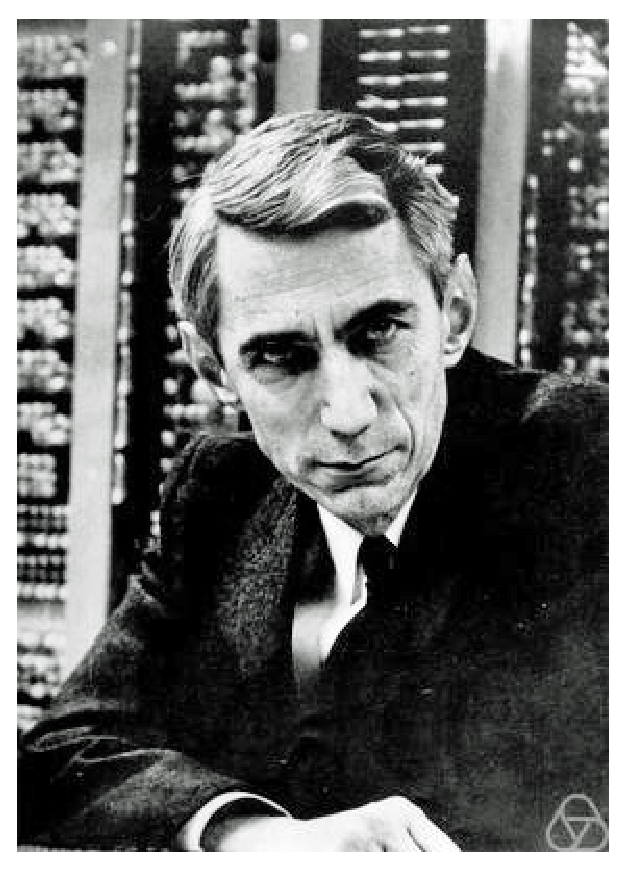
\includegraphics[width=0.8\linewidth]{ClaudeShannon.eps}
    \caption*{\textbf{Claude Shannon} (1916-2001), ingénieur et 
              mathématicien américain. 
              Père fondateur de la théorie de l'information.}
\end{marginfigure}
%-------------------------------------------------------------------------------
%-------------------------------------------------------------------------------
\begin{marginfigure}
    \centering
    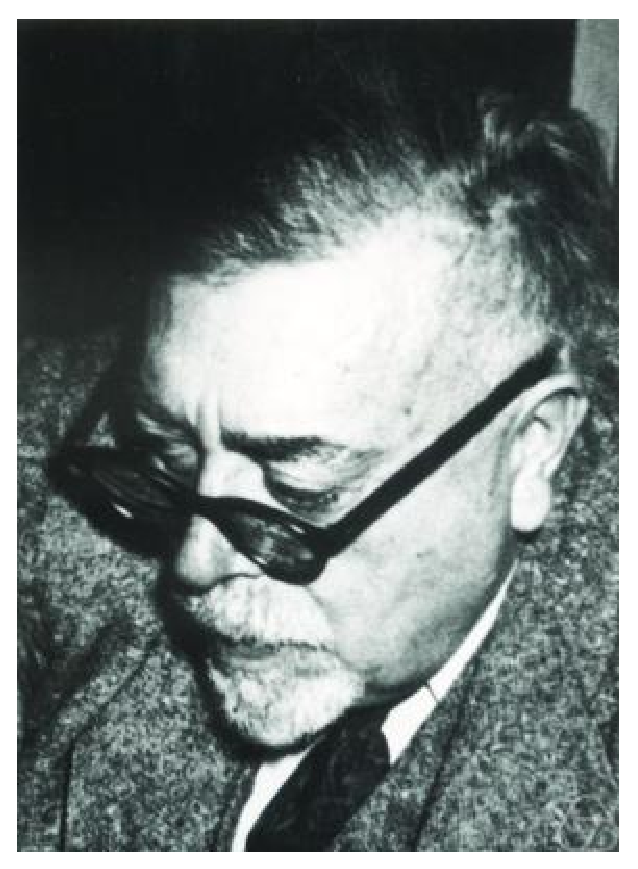
\includegraphics[width=0.8\linewidth]{NorbertWiener.eps}
    \caption*{\textbf{Norbert Wiener} (1894-1964), mathématicien 
              américain. Père fondateur de la cybernétique}
\end{marginfigure}
%-------------------------------------------------------------------------------
%-------------------------------------------------------------------------------
\begin{marginfigure}
    \centering
    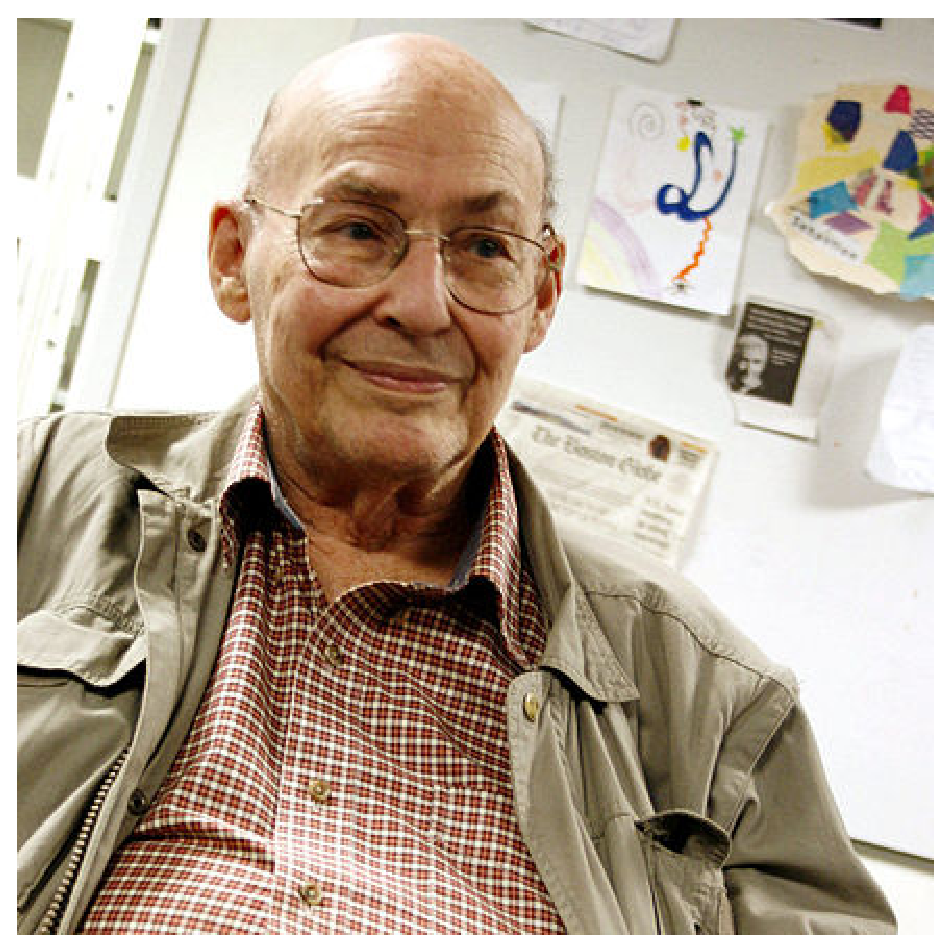
\includegraphics[width=0.8\linewidth]{MarvinMinsky.eps}
    \caption*{\textbf{Marvin Minsky} (1916-2001), mathématicien américain. 
              Auteur de l'expression \og intelligence artificielle\fg}
\end{marginfigure}
%-------------------------------------------------------------------------------

Au niveau structurel, \textbf{un système est un ensemble 
d'éléments constitutifs ayant des relations entre eux et présentant  
une frontière avec son environnement}. Cette définition est parfaitement
représenté par le schéma de la~\cref{fig-systeme}.
Au niveau fonctionnel, \textbf{un système modifie des flux dynamiques 
de matière, d'énergie et d'informations provenant 
de son environnement.}
\index{Système!monovariable}
\index{Système!multivariable}
C'est essentiellement cette dernière définition qui nous sera la plus utile.
Un système sera alors considéré comme une \og boîte\fg traitant une 
ou plusieurs entrées et élaborant une ou plusieurs sorties 
(c.f~\Cref{fig-systeme}). On distinguera les systèmes à 
une entrée et une sortie, dit \textbf{monovariable}\footnote{ou \gls{siso} 
en anglais} des systèmes  a plusieurs entrées et plusieurs sorties, dit 
\textbf{multivariable}\footnote{ou \gls{mimo} en anglais}.

\textbf{L'objectif de ce cours est de permettre la modélisation, 
l'identification et la caractérisation des systèmes monovariables.} 
\`A noter que cet objectif atteint, il nous sera possible de réprésenter 
les systèmes comme des \og boîtes noires\fg pour lesquelles la structure 
interne est inaccessible\footnote{\og Ce qui - en dernière analyse - justifie 
l'attitude ludique, c'est que le seul moyen concevable de dévoiler une 
boîte noire, c'est de jouer avec.\fg (René Thom)}. Une approche basée 
sur la représentation des états internes au système sera 
introduite au dernier chapitre de ce travail~\cref{chap-repreEtat}. 

Pour résumer, nous traiterons dans ce document 
des systèmes monovariables que nous représenterons simplement 
de la façon suivante :
%-------------------------------------------------------------------------------
\begin{center}
    \tikzsetnextfilename{sb_bloc-chap_slci-ext}
    \begin{tikzpicture}
    \sbEntree{E1}
    \sbBloc[3]{B1}{\Large$\Sigma$}{E1}
    \sbRelier[$e(t)$]{E1}{B1}
    \sbSortie[3]{S1}{B1}
    \sbRelier[$s(t)$]{B1}{S1}
\end{tikzpicture}

\end{center}
%-------------------------------------------------------------------------------
où $e(t)$ et $s(t)$ sont respectivement les signaux d'entrée et de sortie 
dépendants du temps et $\Sigma$ est le système traitant l'entrée $e(t)$ et 
élaborant la sortie $s(t)$ délimité par un bloc. 
Cette représentation, dite en \textbf{bloc} ou 
\textbf{schema-bloc}, sera généralisée au~\cref{chap-schemabloc}.
\clearpage
\restoregeometry
\captionsetup{width=0.9\linewidth,labelfont=bf}
%%%%%%%%%%%%%%%%%%%%%%%%%%%%%%%%%%%%%%%%%%%%%%%%%%%%%%%%%%%%%%%%%%%%%%%%%%%%%%%%
%%%%%%%%%%%%%%%%%%%%%%%%%%%%%%%%%%%%%%%%%%%%%%%%%%%%%%%%%%%%%%%%%%%%%%%%%%%%%%%%
\subsection{Propriétés des SLCI}
%%%%%%%%%%%%%%%%%%%%%%%%%%%%%%%%%%%%%%%%%%%%%%%%%%%%%%%%%%%%%%%%%%%%%%%%%%%%%%%%
%%%%%%%%%%%%%%%%%%%%%%%%%%%%%%%%%%%%%%%%%%%%%%%%%%%%%%%%%%%%%%%%%%%%%%%%%%%%%%%%
Les systèmes qui vont nous intéresser dans ce document sont les systèmes
\textbf{linéaires, continus et invariants}. Nous allons ici donner une 
définition de chacune de ces propriétés ainsi que des propriétés secondaires 
que nous rencontrerons au cours de notre étude.
%%%%%%%%%%%%%%%%%%%%%%%%%%%%%%%%%%%%%%%%%%%%%%%%%%%%%%%%%%%%%%%%%%%%%%%%%%%%%%%%
\paragraph{Système linéaire}
%%%%%%%%%%%%%%%%%%%%%%%%%%%%%%%%%%%%%%%%%%%%%%%%%%%%%%%%%%%%%%%%%%%%%%%%%%%%%%%%
\index{Système!linéaire}
Un système est dit linéaire si il respecte les deux principes suivants:
%-------------------------------------------------------------------------------
\begin{itemize}
    \item \emph{Principe de proportionnalité :}
        \textbf{Si $s(t)$ est la réponse à une entrée $e(t)$, alors 
        pour une entrée $\alpha e(t)$ la réponse est $\alpha s(t)$.}
        
        On exprime, schématiquement, ce principe de la façon suivante pour 
        un système linéaire $\Sigma$:
%-------------------------------------------------------------------------------
        \begin{center}
            \tikzsetnextfilename{principe_linearite-chap_slci-ext}
            \input{tikz/principe_linearite-chap_slci.tex}
        \end{center}
%-------------------------------------------------------------------------------
    \item \emph{Principe de superposition :}
        \textbf{Si l'entrée du système se décompose en une somme 
        de plusieurs entrées alors la sortie du système sera la somme des 
        sorties correspondant à chaque entrée séparée.}

        Une nouvelle fois, il est possible d'exprimer ce principe de la façon 
        suivante pour un système linéaire $\Sigma$:
%-------------------------------------------------------------------------------
        \begin{center}
            \tikzsetnextfilename{principe_superposition_1-chap_slci-ext}
            \begin{tikzpicture}
    \begin{scope}[local bounding box=scope1]
        \sbEntree{E1}
        \sbBloc[3]{B1}{\Large$\Sigma$}{E1}
        \node[] at ($(E1.west)+(-0.5,-0.9cm)$) {Si};
        \sbRelier[$e_1(t)$]{E1}{B1}
        \sbSortie[3]{S1}{B1}
        \sbRelier[$s_1(t)$]{B1}{S1}
    \end{scope}
    \begin{scope}[local bounding box=scope2,shift={($(E1)+(0,-2cm)$)}]
        \sbEntree{E2}
        \sbBloc[3]{B2}{\Large$\Sigma$}{E2}
        \sbRelier[$e_2(t)$]{E2}{B2}
        \sbSortie[3]{S2}{B2}
        \sbRelier[$s_2(t)$]{B2}{S2}
    \end{scope}
    \draw[thick,decorate,decoration={brace}] 
    ($(scope2.south west)+(0,0)$) -- ($(scope1.north west)+(0.8,0)$) ;
    \begin{scope}[shift={($(scope1.east)+(1.5,-0.7)$)}]
        \sbEntree{E3}
        \node[] at ($(E3.west)+(-0.5,0)$) {alors};
        \sbBloc[6]{B3}{\Large$\Sigma$}{E3}
        \sbRelier[$e_1(t)+e_2(t)$]{E3}{B3}
        \sbSortie[6]{S3}{B3}
        \sbRelier[$s_1(t)+s_2(t)$]{B3}{S3}
    \end{scope}
\end{tikzpicture}

        \end{center}
%-------------------------------------------------------------------------------
        Notons que ceci reste vrai pour une combinaison linéaire des entrées :
%-------------------------------------------------------------------------------
        \begin{center}
            \tikzsetnextfilename{principe_superposition_2-chap_slci-ext}
            \input{tikz/principe_superposition_2-chap_slci.tex}
        \end{center}
%-------------------------------------------------------------------------------
        avec $\alpha\ \text{et}\ \beta\in\mathbb{R}$, ou un nombre quelconques 
        d'entrées.
        %\[ 
        % s(t)=\sum_{k}^n \alpha_ks_k(t)
        %\]
\end{itemize}
%-------------------------------------------------------------------------------
%%%%%%%%%%%%%%%%%%%%%%%%%%%%%%%%%%%%%%%%%%%%%%%%%%%%%%%%%%%%%%%%%%%%%%%%%%%%%%%%
\paragraph{Système à temps continu}
%%%%%%%%%%%%%%%%%%%%%%%%%%%%%%%%%%%%%%%%%%%%%%%%%%%%%%%%%%%%%%%%%%%%%%%%%%%%%%%%
\index{Système!à temps continu}
\textbf{Un système à temps continu met en oeuvre des signaux 
à temps continus}. Comme nous le verrons, ces signaux seront
modélisés par des fonctions d'une variable continue $t$ de temps.
%%%%%%%%%%%%%%%%%%%%%%%%%%%%%%%%%%%%%%%%%%%%%%%%%%%%%%%%%%%%%%%%%%%%%%%%%%%%%%%%
\paragraph{Système invariant}
%%%%%%%%%%%%%%%%%%%%%%%%%%%%%%%%%%%%%%%%%%%%%%%%%%%%%%%%%%%%%%%%%%%%%%%%%%%%%%%%
\index{Système!invariant}
\textbf{Un système est dit invariant si la sortie ne dépend pas 
explicitement du temps autrement que par l'intermédiaire de l'entrée.}

On représente, schématiquement, un système invariant $\Sigma$, à 
l'aide d'un schéma-bloc ci-dessous 
(avec $\tau$ un temps quelconque.): 
%-------------------------------------------------------------------------------
\begin{center}
    \tikzsetnextfilename{sb_bloc_e3-chap_slci-ext}
    \input{tikz/principe_invariance-chap_slci.tex}
\end{center}
%-------------------------------------------------------------------------------
%%%%%%%%%%%%%%%%%%%%%%%%%%%%%%%%%%%%%%%%%%%%%%%%%%%%%%%%%%%%%%%%%%%%%%%%%%%%%%%%
\paragraph{Système causal}
%%%%%%%%%%%%%%%%%%%%%%%%%%%%%%%%%%%%%%%%%%%%%%%%%%%%%%%%%%%%%%%%%%%%%%%%%%%%%%%%
\index{Système!causal}
%-------------------------------------------------------------------------------
\begin{itemize}
    \item \emph{Principe de causalité :}
        C'est un principe fort de la physique :
        \textbf{\og L'éffet ne précèdant pas sa cause\fg} alors 
        \textbf{\og La réponse du système ne précède pas son excitation\fg}.
        Formellememnt, un système est dit causal si 
        \[ e(t)=0\quad\forall t\le t_0 \Rightarrow s(t)=0\quad\forall t\le t_0\]
\end{itemize}
%-------------------------------------------------------------------------------
%%%%%%%%%%%%%%%%%%%%%%%%%%%%%%%%%%%%%%%%%%%%%%%%%%%%%%%%%%%%%%%%%%%%%%%%%%%%%%%%
\paragraph{Système stable}
%%%%%%%%%%%%%%%%%%%%%%%%%%%%%%%%%%%%%%%%%%%%%%%%%%%%%%%%%%%%%%%%%%%%%%%%%%%%%%%%
\index{Système!stable}
Il existe deux définitions équivalentes de la stabilité pour 
un système linéaire:
%-------------------------------------------------------------------------------
\begin{itemize}
    \item \textbf{Un système est dit stable si à une entrée bornée le système 
        produit une sortie bornée} on parle de stabilité du type \gls{ebsb}.
          \footnote{Chez nos collègues anglo-saxons, 
          on rencontre la notion de BIBO (\og bounded input bounded output\fg)}
    \item \textbf{Un système est dit stable lorsque écarté de sa position 
           d'équilibre, il tend à y revenir}
\end{itemize}
%-------------------------------------------------------------------------------
Nous aurons l'occasion de préciser cette définition par des exemples plus 
concrets lorsque les outils de modélisation des systèmes et des signaux 
auront été introduits. Le \cref{chap-stab} est d'ailleurs totalement dédié 
à l'étude de cette propriété fondamentale.  
%%%%%%%%%%%%%%%%%%%%%%%%%%%%%%%%%%%%%%%%%%%%%%%%%%%%%%%%%%%%%%%%%%%%%%%%%%%%%%%%
%%%%%%%%%%%%%%%%%%%%%%%%%%%%%%%%%%%%%%%%%%%%%%%%%%%%%%%%%%%%%%%%%%%%%%%%%%%%%%%%
%%%%%%%%%%%%%%%%%%%%%%%%%%%%%%%%%%%%%%%%%%%%%%%%%%%%%%%%%%%%%%%%%%%%%%%%%%%%%%%%
\section{Modélisation d'un SLCI}
%%%%%%%%%%%%%%%%%%%%%%%%%%%%%%%%%%%%%%%%%%%%%%%%%%%%%%%%%%%%%%%%%%%%%%%%%%%%%%%%
%%%%%%%%%%%%%%%%%%%%%%%%%%%%%%%%%%%%%%%%%%%%%%%%%%%%%%%%%%%%%%%%%%%%%%%%%%%%%%%%
%%%%%%%%%%%%%%%%%%%%%%%%%%%%%%%%%%%%%%%%%%%%%%%%%%%%%%%%%%%%%%%%%%%%%%%%%%%%%%%%
%%%%%%%%%%%%%%%%%%%%%%%%%%%%%%%%%%%%%%%%%%%%%%%%%%%%%%%%%%%%%%%%%%%%%%%%%%%%%%%%
%%%%%%%%%%%%%%%%%%%%%%%%%%%%%%%%%%%%%%%%%%%%%%%%%%%%%%%%%%%%%%%%%%%%%%%%%%%%%%%%
\subsection{\'Equation différentielle à coefficients constants}
%%%%%%%%%%%%%%%%%%%%%%%%%%%%%%%%%%%%%%%%%%%%%%%%%%%%%%%%%%%%%%%%%%%%%%%%%%%%%%%%
%%%%%%%%%%%%%%%%%%%%%%%%%%%%%%%%%%%%%%%%%%%%%%%%%%%%%%%%%%%%%%%%%%%%%%%%%%%%%%%%
Les systèmes possédant les propriétés précédentes sont dit \textbf{linéaires 
continus et invariants} ou \gls{slci}. Ceux-ci seront modélisés et régis 
par une équation différentielle à coefficients 
constants qui s'écrit dans le cas générale :
%-------------------------------------------------------------------------------
\begin{bequation}[ams align]
\sum_{i=c}^{n}a_i\devi{s(t)}{i}=\sum_{i=0}^{m}b_i\devi{e(t)}{i}
\label{eq-difflci}
\end{bequation}
%-------------------------------------------------------------------------------
avec $n,m,c,\in\mathbb{N}$, $s(t)$ le signal de sortie, $e(t)$ le signal 
d'entrée et $a_i,b_i\in\mathbb{R}$ sont des coefficients constants. 

Le degré de dérivation de la sortie $n$ le plus grand est appelé \textbf{ordre}.
On parlera alors de \textbf{l'ordre du système} $n$. Le paramètre $c$ qui 
correspond au degré de dérivation le plus petit de la sortie est appelé la
\textbf{classe du système}.
%%%%%%%%%%%%%%%%%%%%%%%%%%%%%%%%%%%%%%%%%%%%%%%%%%%%%%%%%%%%%%%%%%%%%%%%%%%%%%%%
\paragraph{Exemples}
%%%%%%%%%%%%%%%%%%%%%%%%%%%%%%%%%%%%%%%%%%%%%%%%%%%%%%%%%%%%%%%%%%%%%%%%%%%%%%%%
Pour un système d'ordre $n=2$, de classe 0 et avec $m=0$, 
son équation différentielle sera alors de la forme :
\[
    a_2\devi{s(t)}{2}+a_1\devi{s(t)}{}+a_0 s(t)=b_0e(t)
\]
%ou encore pour un système d'ordre $n=3$, de classe 
%$c=1$ et avec $m=1$, l'équation différentielle sera de la forme :
%\[
%    a_3\devi{s(t)}{3}+a_2\devi{s(t)}{2}+a_1\devi{s(t)}{}
%    =b_0e(t)+b_1\devi{e(t)}{}
%\]
\input{re/newgeometry}
\captionsetup{width=0.9\linewidth,labelfont=bf}
%%%%%%%%%%%%%%%%%%%%%%%%%%%%%%%%%%%%%%%%%%%%%%%%%%%%%%%%%%%%%%%%%%%%%%%%%%%%%%%%
%%%%%%%%%%%%%%%%%%%%%%%%%%%%%%%%%%%%%%%%%%%%%%%%%%%%%%%%%%%%%%%%%%%%%%%%%%%%%%%%
\subsection{Exemples de mises en équation}
%%%%%%%%%%%%%%%%%%%%%%%%%%%%%%%%%%%%%%%%%%%%%%%%%%%%%%%%%%%%%%%%%%%%%%%%%%%%%%%%
%%%%%%%%%%%%%%%%%%%%%%%%%%%%%%%%%%%%%%%%%%%%%%%%%%%%%%%%%%%%%%%%%%%%%%%%%%%%%%%%
Pour un problème donné, ces équations différentielles proviennent 
directement de la modélisation de la physique (qu'il soit mécanique, 
électronique, thermique \ldots).
Par exemple, dans le cas d'un problème de mécanique, 
c'est la relation fondamentale de la dynamique qui est 
la source importante d'équations différentielles (appelées équations 
du mouvement).
En électronique, ce sont, par exemple, les lois des noeuds et mailles (ou 
lois de Kirchhoff) qui permettront d'écrire ces équations différentielles. 
%%%%%%%%%%%%%%%%%%%%%%%%%%%%%%%%%%%%%%%%%%%%%%%%%%%%%%%%%%%%%%%%%%%%%%%%%%%%%%%%
\paragraph{Décharge d'un condensateur\label{para-decharge}}
%%%%%%%%%%%%%%%%%%%%%%%%%%%%%%%%%%%%%%%%%%%%%%%%%%%%%%%%%%%%%%%%%%%%%%%%%%%%%%%%
Considérons le circuit ouvert ci-contre, initialement chargé, constitué 
d'un condensateur de capacité électrique $C$ et d'une résistance de valeur $R$. 
À la fermeture de l'interrupteur, à $t=0$, un courant $i(t)$ parcourt 
le circuit. On observe alors la décharge du condensateur à travers 
une resistance $R$. 

On souhaite suivre la quantité de charge $q(t)$ aux bornes du condensateur au 
cours du temps.
%-------------------------------------------------------------------------------
\begin{marginfigure}[-8em]   
    \centering
    \tikzsetnextfilename{decharge_condensateur-chap_slci-ext}
    %               K           
%     A ------B    C---------D
%     |                      |
%     |                      |
% C1--E--C2                --J-R2 
%                          |   |
% C3--F--C4               R1-I--
%     |                      |
%     |                      |
%     G----------------------H
%
%
\begin{tikzpicture}

    \pgfmathsetmacro{\pC}{0.75}   % distance de C(1,2,3,4) en x relativement E/F
    \pgfmathsetmacro{\eC}{0.5}    % ecartement du condensateur E-F
    \pgfmathsetmacro{\lR}{1.25}   % longueur de la resistance
    \pgfmathsetmacro{\pR}{0.25}   % position de R1 / I
    \pgfmathsetmacro{\eR}{2*\pR}
    \pgfmathsetmacro{\ab}{1.5}
    \pgfmathsetmacro{\cb}{1.0}
    \pgfmathsetmacro{\gh}{2*\ab+\cb}
    \pgfmathsetmacro{\fg}{1}
    \pgfmathsetmacro{\tmpu}{0.5*\eC}
    \pgfmathsetmacro{\tmpd}{-0.5*\lR}
    \pgfmathsetmacro{\dj}{\fg+\tmpu+\tmpd}

    \coordinate (A)  at (0,0);
    \coordinate (B)  at ($(A)+(\ab,0)$);
    \coordinate (C)  at ($(B)+(\cb,0)$);
    \coordinate (D)  at ($(C)+(\ab,0)$);
    \coordinate (E)  at ($(A)+(0,-\fg)$);
    \coordinate (F)  at ($(E)+(0,-\eC)$);
    \coordinate (C1) at ($(E)+(-\pC,0)$);
    \coordinate (C2) at ($(E)+(\pC,0)$);
    \coordinate (C3) at ($(F)+(-\pC,0)$);
    \coordinate (C4) at ($(F)+(\pC,0)$);
    \coordinate (G)  at ($(F)+(0,-\fg)$);
    \coordinate (H)  at ($(G)+(\gh,0)$);
    \coordinate (I)  at ($(H)+(0,\dj)$);
    \coordinate (J)  at ($(I)+(0,\lR)$);
    \coordinate (K)  at ($(C)+(-0.75,0.5)$);
    \coordinate (R1) at ($(I)+(-\pR,0)$);
    \coordinate (R2) at ($(R1)+(\eR,\lR)$);

    %\node[circle,fill=white,draw=black,ultra thick] at (B) {};
    \draw[thick] (A)  -- (B);
    \draw[thick] (C)  -- (D);
    \draw[thick] (A)  -- (E);
    \draw[very thick,col1] (C1) -- (C2) 
    node[col1,xshift=1em,yshift=-0.5em] {$C$};
    \draw[very thick,col1] (C3) -- (C4);
    \draw[thick] (F)  -- (G);
    \draw[thick] (G)  -- (H);
    \draw[thick] (I)  -- (H);
    \draw[thick] (J)  -- (D);
    \draw[thick] (K)  -- (C);
    \draw[very thick,col4] (R1) rectangle (R2) 
    node[yshift=-1.5em,xshift=0.75em] {$R$};
    \draw[draw=black,fill=white] (B) circle (2pt);
    \draw[draw=black,fill=white] (C) circle (2pt);
\end{tikzpicture}

    \caption{Circuit RC ouvert.\label{fig-decharge_condensateur}}
\end{marginfigure}
%-------------------------------------------------------------------------------
La somme des tensions aux bornes du condensateur et de la résistance 
étant nulle, on a :
%-------------------------------------------------------------------------------
\begin{align*}
    R\devi{q(t)}{}+\dfrac{1}{C}q(t)=0 
\end{align*}
%-------------------------------------------------------------------------------
Comme précédemment, on identifie formellemet cette équation différentielle 
à la forme générale de l'\cref{eq-difflci} avec $s(t)=q(t)$, $e(t)=0$, 
$n=$1, $m=0$, $a_1=R$, $a_0=\dfrac{1}{C}$.

Nous laissons au lecteur la résolution de cette équation différentielle 
par une approche direct classique. Sa résolution utilisant la transformée 
de Laplace, est présenté en exercice à la fin de ce chapitre.
%Nous la rencontrerons à nouveau au~\cref{chap-model}, après avoir 
%présenté la méthode générale pour la résolution de ce type d'équation.
%%%%%%%%%%%%%%%%%%%%%%%%%%%%%%%%%%%%%%%%%%%%%%%%%%%%%%%%%%%%%%%%%%%%%%%%%%%%%%%%
\paragraph{Système masse-ressort\label{para-masse_ressort}}
%%%%%%%%%%%%%%%%%%%%%%%%%%%%%%%%%%%%%%%%%%%%%%%%%%%%%%%%%%%%%%%%%%%%%%%%%%%%%%%%
On considère un système mécanique constitué d'une masse $m$ en translation 
couplée avec un ressort de constante
de raideur $k$ et un amortisseur de coefficient de frottement 
visqueux $b$ (c.a.d que la force est 
proportionnelle à la vitesse). 
La masse est soumise à une force $\vect{f}=f(t)\zz{}$.
%-------------------------------------------------------------------------------
\begin{marginfigure}[-8em]
    \centering
    \tikzsetnextfilename{masse_ressort-chap_slci-ext}
    \input{tikz/masse_ressort-chap_slci.tex}
    \caption{(gauche) Système masse-ressort. (droite) Schéma-bloc de ce même 
    système.
    \label{fig-masse-ressort}}
\end{marginfigure}
%-------------------------------------------------------------------------------
En appliquant le principe fondamentale de la dynamique en projection 
sur le vecteur $\zz{}$, on obtient l'équation du mouvement suivante :
\[
m\devi{z(t)}{2}+b\devi{z(t)}{}+kz(t)=f(t)
\]
\newpage
\restoregeometry
\captionsetup{width=0.9\linewidth,labelfont=bf}
La résolution de cette équation du mouvement permet de connaitre la position 
de la masse à chaque instant connaissant la force exterieur 
appliquée $f(t)$. Le système masse-ressort peut être assimilé à un~\gls{slci} 
dont l'entrée $e(t)$ est la force $f(t)$ et la sortie $s(t)$ est la 
position $z(t)$ de la masse (c.f le schéma-bloc de la \cref{fig-masse-ressort})

On identifie simplement, cette équation différentielle à la forme générale 
de l'\cref{eq-difflci} pour $s(t)=z(t)$, $e(t)=f(t)$, 
$n=$2, $m=0$, $a_2=m$, $a_1=b$, $a_0=k_r$ et $b_0=$1.
La résolution complète sera donnée en exercice à la fin de ce chapitre.
%%%%%%%%%%%%%%%%%%%%%%%%%%%%%%%%%%%%%%%%%%%%%%%%%%%%%%%%%%%%%%%%%%%%%%%%%%%%%%%%
%%%%%%%%%%%%%%%%%%%%%%%%%%%%%%%%%%%%%%%%%%%%%%%%%%%%%%%%%%%%%%%%%%%%%%%%%%%%%%%%
%%%%%%%%%%%%%%%%%%%%%%%%%%%%%%%%%%%%%%%%%%%%%%%%%%%%%%%%%%%%%%%%%%%%%%%%%%%%%%%%
\section{Modélisation d'un signal}
%%%%%%%%%%%%%%%%%%%%%%%%%%%%%%%%%%%%%%%%%%%%%%%%%%%%%%%%%%%%%%%%%%%%%%%%%%%%%%%%
%%%%%%%%%%%%%%%%%%%%%%%%%%%%%%%%%%%%%%%%%%%%%%%%%%%%%%%%%%%%%%%%%%%%%%%%%%%%%%%%
%%%%%%%%%%%%%%%%%%%%%%%%%%%%%%%%%%%%%%%%%%%%%%%%%%%%%%%%%%%%%%%%%%%%%%%%%%%%%%%%
\textbf{Un signal est une variation d'une grandeur qui porte l'information 
de la sollicitation ou de la réponse d'un système.}

Les signaux continus sont modélisés mathématiquement par des fonctions 
continues du temps. Formellement, par une fonction $s$ telle que :
%-------------------------------------------------------------------------------
\begin{align*}
s : \mathbb{R}&\rightarrow\mathbb{R} \\  
t&\rightarrow s(t) 
\end{align*}    
%-------------------------------------------------------------------------------
Il existe cependant d'autres types de signaux qui sont très souvent confondus 
à tort:
%-------------------------------------------------------------------------------
\begin{itemize}
    \item un signal \emph{quantifié} est un signal continu 
          dont la valeur ne peut prendre que des valeurs discrètes. 
    \item un signal \emph{discret} est un signal à temps discret.
    \item un signal \emph{numérique} est un signal discret et quantifié.   
\end{itemize}
%-------------------------------------------------------------------------------
\textbf{Dans le reste de ce document, nous ne traiterons que
du cas de signaux en temps continu}. Les signaux en temps discret
sont généralement abordées lors d'un cours 
avancé d'automatique en cycle ingénieur.
%\newpage
%%%%%%%%%%%%%%%%%%%%%%%%%%%%%%%%%%%%%%%%%%%%%%%%%%%%%%%%%%%%%%%%%%%%%%%%%%%%%%%%
%%%%%%%%%%%%%%%%%%%%%%%%%%%%%%%%%%%%%%%%%%%%%%%%%%%%%%%%%%%%%%%%%%%%%%%%%%%%%%%%
\subsection{Propriétés des signaux continus}
%%%%%%%%%%%%%%%%%%%%%%%%%%%%%%%%%%%%%%%%%%%%%%%%%%%%%%%%%%%%%%%%%%%%%%%%%%%%%%%%
%%%%%%%%%%%%%%%%%%%%%%%%%%%%%%%%%%%%%%%%%%%%%%%%%%%%%%%%%%%%%%%%%%%%%%%%%%%%%%%%
%%%%%%%%%%%%%%%%%%%%%%%%%%%%%%%%%%%%%%%%%%%%%%%%%%%%%%%%%%%%%%%%%%%%%%%%%%%%%%%%
\paragraph{Causal}
%%%%%%%%%%%%%%%%%%%%%%%%%%%%%%%%%%%%%%%%%%%%%%%%%%%%%%%%%%%%%%%%%%%%%%%%%%%%%%%%
\index{Signal!causal}
Un signal modélisé par la fonction $s(t)$ est dit \textbf{causal}
si ce signal est nul pour tout $t<0$. Pour un signal en entrée, le temps 
$t=0$ permet de définir une origine des temps.
%-------------------------------------------------------------------------------
\begin{figure}[!h]
    \centering
    \tikzsetnextfilename{causal-chap_slci-ext}
    \input{tikz/causal-chap_slci.tex}
\end{figure}
%-------------------------------------------------------------------------------
%%%%%%%%%%%%%%%%%%%%%%%%%%%%%%%%%%%%%%%%%%%%%%%%%%%%%%%%%%%%%%%%%%%%%%%%%%%%%%%%
\paragraph{Retardé}
%%%%%%%%%%%%%%%%%%%%%%%%%%%%%%%%%%%%%%%%%%%%%%%%%%%%%%%%%%%%%%%%%%%%%%%%%%%%%%%%
\index{Signal!retardé}
Un signal $s(t-\tau)$ est dit \textbf{retardé} d'un temps $\tau$ 
par rapport à $s(t)$, si on lui a fait subir un changement
d'origine des temps par rapport au signal $s(t)$.
%-------------------------------------------------------------------------------
\begin{center}
    \tikzsetnextfilename{retarde-chap_slci-ext}
    \input{tikz/retarde-chap_slci.tex}
\end{center}
%-------------------------------------------------------------------------------
%%%%%%%%%%%%%%%%%%%%%%%%%%%%%%%%%%%%%%%%%%%%%%%%%%%%%%%%%%%%%%%%%%%%%%%%%%%%%%%%
\paragraph{Périodique}
%%%%%%%%%%%%%%%%%%%%%%%%%%%%%%%%%%%%%%%%%%%%%%%%%%%%%%%%%%%%%%%%%%%%%%%%%%%%%%%%
\index{Signal!périodique}
Un signal est dit \textbf{périodique} s'il se reproduit identique à lui
même au bout d'un même intervalle de temps ou periode $T$. On définit alors 
sa fréquence $f=1/T$ qui est l'inverse de la période $T$ ou la pulsation 
$\omega$ définie par rapport au cercle unité $\omega=2\pi f$.
%-------------------------------------------------------------------------------
\begin{figure}[!htb]
    \centering
    \tikzsetnextfilename{periodique-chap_slci-ext}
    \begin{tikzpicture}
    \begin{axis}
    [	ticks=none,
        axis line style = thick,
        height=5cm,
        width=9cm,
        axis x line=center,
        axis y line=center,
        xmin=-2,
        xmax=16,
        ymin=-2.0,
        ymax=2.0,
        xlabel={$t$},
        ylabel={$s(t)$},
        xlabel style={below right},
        ylabel style={above left},
        clip bounding box=upper bound,
        enlargelimits=false
    ]
    \addplot[very thick,col1,domain=-2:0, samples=101] {0};
    \addplot[very thick,col1,domain=0:2, samples=101]  {0.5*x};
    \addplot[very thick,col1,domain=2:6, samples=101]  {-0.5*x+2};
    \addplot[very thick,col1,domain=6:10, samples=101] {0.5*x-4};
    \addplot[very thick,col1,domain=10:14, samples=101]{-0.5*x+6};
    \draw[col1] (axis cs:2,1) -- (axis cs:2,1.25);
    \draw[col1] (axis cs:10,1) -- (axis cs:10,1.25);
    \draw[col1,ultra thick, latex-latex] (axis cs:2,1.25) -- 
    node[above,yshift=+0.2em]{$T$} (axis cs:10,1.25);
    \end{axis}
\end{tikzpicture}

\end{figure}
%-------------------------------------------------------------------------------
Le signal complet peut être totalement d'écrit en considérant un motif de base 
$s_0(t)$ tel que
%-------------------------------------------------------------------------------
\begin{align*}
    s_0(t) =
    \begin{dcases}
        s(t)&\quad\text{pour}\quad 0\le t\le T   \\
        0&\quad\text{pour}\quad t>T
    \end{dcases}
\end{align*}
%-------------------------------------------------------------------------------
Le signal $s(t)$ est alors la somme (série) du motif retardé de $nT$ 
avec $n\in\mathbb{N}$ tel que :
\[
s(t)=\sum_0^\infty s_0(t-nT)
\]
L'analyse de Fourier est un outil fondamental pour l'étude 
de ces signaux périodiques. Elle sort cependant légèrement du cadre de 
ce cours. (c.f~\Cref{annexe-seriefourier}).
%%%%%%%%%%%%%%%%%%%%%%%%%%%%%%%%%%%%%%%%%%%%%%%%%%%%%%%%%%%%%%%%%%%%%%%%%%%%%%%%
\paragraph{Stable}
%%%%%%%%%%%%%%%%%%%%%%%%%%%%%%%%%%%%%%%%%%%%%%%%%%%%%%%%%%%%%%%%%%%%%%%%%%%%%%%%
\index{Signal!stable}
En se basant sur la définition donnée d'un système stable.
Nous ne limiterons à dire qu'un signal stable est un signal 
borné. Les signaux usuels en entrée de nos systèmes sont bornés 
et stables.

La~\cref{fig-stabilite_signaux} présente un exemple qualitatif de réponses 
stables et instables pour deux sollicitations bornées (respectivement une 
sollicitation constante et une sollicitation oscillante).
%-------------------------------------------------------------------------------
\begin{figure}[!ht]
    \centering
    \tikzsetnextfilename{entree_echelon-chap_slci_ext}
    \input{tikz/entree_echelon-chap_slci.tex}
    \tikzsetnextfilename{stable_echelon-chap_slci_ext}
    \input{tikz/stable_echelon-chap_slci.tex}
    \tikzsetnextfilename{instable_echelon-chap_slci_ext}
    \begin{tikzpicture}
    \begin{axis}
    [	ticks=none,
        axis line style = thick,
        height=5cm,
        width=5cm,
        axis x line=center,
        axis y line=center,
        xmin=-2,
        xmax=10,
        ymin=-0.5,
        ymax=2.0,
        xlabel={$t$},
        ylabel={$s(t)$},
        xlabel style={below right},
        ylabel style={above left},
    ]
    \addplot[signalr,domain=-2:0]  {0};
    \addplot[signalr,domain=0:10] {0.05*x^2};
    \end{axis}
\end{tikzpicture}


    \tikzsetnextfilename{entree_harm-chap_slci_ext}
    \begin{tikzpicture}
    \begin{axis}
    [   ticks=none,
        axis line style = thick,
        height=5cm,
        width=5cm,
        axis x line=center,
        axis y line=center,
        xmin=-2,
        xmax=10,
        ymin=-2.0,
        ymax=2.0,
        xlabel={$t$},
        ylabel={$e(t)$},
        xlabel style={below right},
        ylabel style={above left},
    ]
    \addplot[signaln,domain=-2:0]  {0};
    \addplot[signaln,domain=0:9.5]  {sin(deg(2*x))};
    \end{axis}
\end{tikzpicture}

    \tikzsetnextfilename{stable_harm-chap_slci_ext}
    \input{tikz/stable_harm-chap_slci.tex}
    \tikzsetnextfilename{instable_harm-chap_slci_ext}
    \begin{tikzpicture}%
    \begin{axis}
    [	ticks=none,
        axis line style = thick,
        height=5cm,
        width=5cm,
        axis x line=center,
        axis y line=center,
        xmin=-2,
        xmax=10,
        ymin=-5,
        ymax=5,
        xlabel={$t$},
        ylabel={$s(t)$},
        xlabel style={below right},
        ylabel style={above left},
    ]
    \addplot[signalr,domain=-2:0]  {0};
    \addplot[signalr,domain=0:9.5] {0.8*sin(3*deg(x))*exp(0.2*x)};
    \end{axis}
\end{tikzpicture}

    \caption{Trois exemples de réponses d'un SLCI à des sollicitations bornées :
            (en bleu)  réponses stables 
            (en rouge) réponses instables.\label{fig-stabilite_signaux}}
\end{figure}
%-------------------------------------------------------------------------------
\newpage
\input{re/newgeometry}
\captionsetup{width=0.9\linewidth,labelfont=bf}
%%%%%%%%%%%%%%%%%%%%%%%%%%%%%%%%%%%%%%%%%%%%%%%%%%%%%%%%%%%%%%%%%%%%%%%%%%%%%%%%
%%%%%%%%%%%%%%%%%%%%%%%%%%%%%%%%%%%%%%%%%%%%%%%%%%%%%%%%%%%%%%%%%%%%%%%%%%%%%%%%
\subsection{Signaux usuels rencontrés\ldots\label{sec-signaux_usuels}}
%%%%%%%%%%%%%%%%%%%%%%%%%%%%%%%%%%%%%%%%%%%%%%%%%%%%%%%%%%%%%%%%%%%%%%%%%%%%%%%%
%%%%%%%%%%%%%%%%%%%%%%%%%%%%%%%%%%%%%%%%%%%%%%%%%%%%%%%%%%%%%%%%%%%%%%%%%%%%%%%%
%Nous aurons l'occasion de rencontrer de nombreuses fois certains signaux.
Certains signaux sont des briques de base pour la construction de
signaux plus complexes. Il est alors essentiel de bien les caractériser.
Ici, nous distinguons les signaux généralement utilisés en 
entrée des signaux généralement rencontrées en sortie des \gls{slci}.
%%%%%%%%%%%%%%%%%%%%%%%%%%%%%%%%%%%%%%%%%%%%%%%%%%%%%%%%%%%%%%%%%%%%%%%%%%%%%%%%
\subsubsection{\ldots en entrée}
%%%%%%%%%%%%%%%%%%%%%%%%%%%%%%%%%%%%%%%%%%%%%%%%%%%%%%%%%%%%%%%%%%%%%%%%%%%%%%%%
%%%%%%%%%%%%%%%%%%%%%%%%%%%%%%%%%%%%%%%%%%%%%%%%%%%%%%%%%%%%%%%%%%%%%%%%%%%%%%%%
\paragraph{Impulsion de Dirac\index{Signaux usuels!Impulsion de Dirac}}
%%%%%%%%%%%%%%%%%%%%%%%%%%%%%%%%%%%%%%%%%%%%%%%%%%%%%%%%%%%%%%%%%%%%%%%%%%%%%%%%
L'impulsion de Dirac
$\delta(t)$ est une \og fonction\fg 
\footnote{Les guillemets sont essentiels pour ne pas se fâcher avec 
nos collègues mathématiciens. En effet, ce signal est un exemple classique de 
la théorie des distributions qui étend la notion de fonction.} telle que
%-------------------------------------------------------------------------------
\begin{marginfigure}
    \centering
    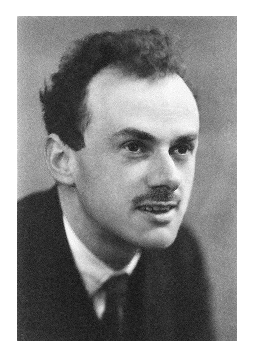
\includegraphics[width=0.9\linewidth]{PaulDirac.eps} 
    \caption{\index{Dirac, Paul}\textbf{Paul Dirac}, (1902-1984) 
              mathématicien et physicien britannique. Auteur de 
              contributions majeures en mécanique quantique. 
              \href{https://www.youtube.com/watch?v=H7mOU1Xu-yA}{Lien Youtube}
              } 
\end{marginfigure}
%-------------------------------------------------------------------------------
%-------------------------------------------------------------------------------
\begin{align*}
    \delta(t) : 
    \begin{dcases}
    	\int\limits_{-\infty}^{+\infty}	 \delta(t)\,\,\dd{t}&=1   \\
        \int\limits_{-\infty}^{+\infty}  \delta(t)f(t)\,\,\dd{t}&=f(0)	
    \end{dcases}
\end{align*}
%-------------------------------------------------------------------------------
Cette fonction est donc nulle partout sauf en $t=0$ où elle prend 
une valeur infinie. C'est pourquoi l'intégrale sur tous les nombres réels 
d'une impulsion de Dirac est normalisée à 1.
Graphiquement une impulsion de Dirac $\delta(t)$ est 
représentée par une flèche en $t=0$. La figure ci-dessous présente 
une impulsion de Dirac ainsi qu'une 
impulsion retardée de $\tau$ noté $\delta(t-\tau)$.
%-------------------------------------------------------------------------------
\begin{figure}[!h]
    \centering
    \tikzsetnextfilename{dirac-chap_slci-ext}
    \input{tikz/dirac-chap_slci.tex}
\end{figure}
%-------------------------------------------------------------------------------
L'impulsion de Dirac peut être expérimentalement approchée par un signal 
bref et de grande amplitude. La figure~\ref{fig-dirac2} représente un modèle 
approchée de l'impulsion de Dirac. Il est possible de montrer que cette fonction
$\delta_a(t)$ s'approche d'une impulsion de Dirac lorsque $a\to0$.
%-------------------------------------------------------------------------------
\begin{marginfigure}
    \centering
    \tikzsetnextfilename{dirac_reel-chap_slci-ext}
    \input{tikz/dirac_reel-chap_slci.tex}
    \caption{Représentation de l'impulsion de Dirac approchée. 
             Celle-ci tend vers l'impulsion de Dirac pour $a\to0$. 
             On remarquera que l'aire du rectangle est toujours égale à 1.
             \label{fig-dirac2}}
\end{marginfigure}
%-------------------------------------------------------------------------------

Nous rencontrerons quelque fois l'impulsion de Dirac sous sa forme généralisée, 
\[
e(t)=E_0\delta(t)
\]
où $e(t)$ est le signal d'entrée du système et $E_0$ la valeur de l'amplitude 
de l'impulsion de Dirac dont la dimension dépendra de la nature du 
problème considéré.
La réponse d'un système à une impulsion de Dirac est appelée 
\textbf{réponse impulsionnelle}.
Nous verrons par la suite qu'une telle sollicitation brève et de grande 
amplitude permet de parfaitement caractériser le système. La réponse 
impulsionnelle, qui en résulte, contient toute l'information sur le système 
linéaire qui l'a élaboré.
%%%%%%%%%%%%%%%%%%%%%%%%%%%%%%%%%%%%%%%%%%%%%%%%%%%%%%%%%%%%%%%%%%%%%%%%%%%%%%%%
\paragraph{\'Echelon-unité}
%%%%%%%%%%%%%%%%%%%%%%%%%%%%%%%%%%%%%%%%%%%%%%%%%%%%%%%%%%%%%%%%%%%%%%%%%%%%%%%%
\index{Signaux usuels!échelon unité}
L'échelon-unité est défini par la fonction, noté $u(t)$, telle que :
\[
    u(t)=
    \begin{cases} 
    0 \qquad \forall t<0    \\ 
    1 \qquad \forall t\geq 0 
    \end{cases}
\]
Cette fonction présente une marche\footnote{Nos 
collègues anglo-saxons l'appelle la \og\emph{step function}\fg} à $t=0$. 
Ci contre, nous la représentons avec la fonction retardée $u(t-\tau)$.
%-------------------------------------------------------------------------------
\begin{marginfigure}
    \centering
    \tikzsetnextfilename{echelon-chap_slci-ext}
    \input{tikz/echelon-chap_slci.tex}
    \caption{Représentation graphique de (haut) la fonction échelon-unité 
             et (bas) la fonction échelon-unité retardée de $\tau$
            \label{fig-echelon}}
\end{marginfigure}
%-------------------------------------------------------------------------------
En général, l'échelon-unité est utilisé en entrée de nos systèmes pour 
modéliser des états fermé/ouvert (\og on/off\fg) ou encore en régulation.
Nous la rencontrerons souvent sous sa forme généralisée, 
\[
    e(t)=E_0u(t)
\]
où $e(t)$ est le signal d'entrée du système et $E_0$ la valeur seuil 
de l'échelon dont la dimension dépend de la nature du problème considéré.

D'après les propriétés du signal échelon-unité et de la causalité, il 
est possible de rendre causale une fonction quelconque en la 
multipliant par un échélon-unité (c.f \ref{subsec:decomp_usuels}).

La réponse d'un système à un échelon est appelée 
\textbf{réponse indicielle}.

Remarquons que la fonction échelon-unité est l'intégrale 
de la distribution de Dirac,
%-------------------------------------------------------------------------------
\begin{equation}
    u(t)=\int\limits_{-\infty}^{t} \delta(\tau)\,\,\dd{\tau}
    \label{eq-echelon-dirac_relation}
\end{equation}
%-------------------------------------------------------------------------------
%-------------------------------------------------------------------------------
\begin{marginfigure}
    \centering
    \tikzsetnextfilename{rampe-chap_slci-ext}
    \begin{tikzpicture}
    \begin{axis}[
    name=ax2,
    ticks=none,
    axis line style = thick,
    height=4cm,
    width=5cm,
    axis x line=center,
    axis y line=center,
    xmin=-2,
    xmax=6,
    ymin=-1.5,
    ymax=6,
    xlabel={$t$},
    ylabel={$r(t)$},
    xlabel style={below right},
    ylabel style={above left},
    ]
    \addplot [ultra thick,col1,domain=-2:0, samples=101]{0};
    \addplot [ultra thick,col1,domain=0:15, samples=101]{x};
    \end{axis}
    \begin{axis}[
    at={(ax2.below south west)},
    anchor=north west,
    yshift=-0.9em,
    axis line style = thick,
    height=4cm,
    width=5cm,
    axis x line=center,
    axis y line=center,
    xmin=-2,
    xmax=8,
    ymin=-1.5,
    ymax=8,
    xlabel={$t$},
    ylabel={$r(t-\tau)$},
    xlabel style={below right},
    ylabel style={above left},
    xticklabels={$\tau$},
    xtick={2},
    ytick=\empty,
    ]
    \addplot [ultra thick,col1,domain=-2:2, samples=101]{0};
    \addplot [ultra thick,col1,domain=2:17, samples=101]{x-2};
    \end{axis}
\end{tikzpicture}

    \caption{Représentation graphique de (haut) la fonction rampe-unité et 
                                     (bas) la fonction rampe-unité retardée
                                     de $\tau$\label{fig-rampe}}
\end{marginfigure}
%-------------------------------------------------------------------------------
%%%%%%%%%%%%%%%%%%%%%%%%%%%%%%%%%%%%%%%%%%%%%%%%%%%%%%%%%%%%%%%%%%%%%%%%%%%%%%%%
\paragraph{Rampe-unité}
%%%%%%%%%%%%%%%%%%%%%%%%%%%%%%%%%%%%%%%%%%%%%%%%%%%%%%%%%%%%%%%%%%%%%%%%%%%%%%%%
\index{Signaux usuels!rampe unité}
Le signal rampe-unité\footnote{On retrouve parfois~\cite{sueurautomatique} 
le terme d'échelon vitesse pour désigner la fonction rampe} est
modélisé par la fonction $r(t)$ telle que :
\[
    r(t)=
    \begin{cases}
	0\,\,\,\,t<0 \\
	t\,\,\,\,t\geq0 
    \end{cases}
\]
ou autrement dit, en utilisant la propriété de causalité de l'échelon:
\[
    r(t)=t\cdot u(t)
\]
Remarquons que la fonction rampe est l'intégrale de l'échelon-unité, notamment 
%-------------------------------------------------------------------------------
\begin{equation}
    r(t)=\int\limits_{-\infty}^{t} u(\tau)\,\,\dd{\tau}
    \label{eq-rampe-echelon_relation}
\end{equation}
%-------------------------------------------------------------------------------
La réponse d'un système à une rampe ne possède pas de nom spécifique 
pour la distinguer des autres réponses. Nous parlerons donc simplement 
de \textbf{réponse à une rampe}. 
%%%%%%%%%%%%%%%%%%%%%%%%%%%%%%%%%%%%%%%%%%%%%%%%%%%%%%%%%%%%%%%%%%%%%%%%%%%%%%%%
\paragraph{Sinuso\"ide}
%%%%%%%%%%%%%%%%%%%%%%%%%%%%%%%%%%%%%%%%%%%%%%%%%%%%%%%%%%%%%%%%%%%%%%%%%%%%%%%%
\index{Signaux usuels!sinuso\"ide}
Le signal périodique sinuso\"idal $s(t)$ est la fonction telle que :
\[
    s(t)=A\sin{(\omega t +\phi)}\cdot u(t)
\]
avec $A$ son amplitude, $\omega$ sa pulsation (en \si{\radian\per\second}) 
et $\phi$ sa phase (\si{\radian}).
%La pulsation permet de définir la fréquence $f=\dfrac{\omega}{2\pi}$ 
%en \si{\hertz}, elle même liée à la période $T=\dfrac{1}{f}$ en 
%\si{\second}.
%-------------------------------------------------------------------------------
\begin{marginfigure}
    \centering
    \tikzsetnextfilename{sinusoide-chap_slci-ext}
    \resizebox{\linewidth}{!}{\input{tikz/sinusoide-chap_slci.tex}}
    \caption{Représentation de signaux sinuso\"idaux de même pulsation 
             et amplitude. (bleu) de phase $\phi=0$ et 
            (rouge) de phase $\phi=-\dfrac{\pi}{2}$.\label{fig-sin}}
\end{marginfigure}
%-------------------------------------------------------------------------------
Il est possible de voir le signal sinuso\"idal comme la combinaison
linéaire de la fonction cosinus et sinus. En effet, en utilisant une 
des rélations trigonométriques simples\footnote{à savoir la comptine des 
lycéens $\sin(a+b)=\sin{a}\cos{b}+\sin{b}\cos{a}$}, $s(t)$ s'écrit :
\[
    s(t)=A(\sin(\phi)\cos{\omega t}+\cos(\phi)\sin{\omega t})
\]
La réponse d'un système à une sinuso\"ide est appelée la 
\textbf{réponse harmonique} et son analyse fera l'objet de tout 
un chapitre (\Cref{chap-repfreq}).

Le~\cref{tab-sin_deph} rappel la terminologie associé au déphasage entre 
deux signaux sinuso\"idaux. 
%%%%%%%%%%%%%%%%%%%%%%%%%%%%%%%%%%%%%%%%%%%%%%%%%%%%%%%%%%%%%%%%%%%%%%%%%%%%%%%%
\subsubsection{\ldots en sortie}
%%%%%%%%%%%%%%%%%%%%%%%%%%%%%%%%%%%%%%%%%%%%%%%%%%%%%%%%%%%%%%%%%%%%%%%%%%%%%%%%
%%%%%%%%%%%%%%%%%%%%%%%%%%%%%%%%%%%%%%%%%%%%%%%%%%%%%%%%%%%%%%%%%%%%%%%%%%%%%%%%
\paragraph{Exponentielle décroissante}
%%%%%%%%%%%%%%%%%%%%%%%%%%%%%%%%%%%%%%%%%%%%%%%%%%%%%%%%%%%%%%%%%%%%%%%%%%%%%%%%
\index{Signaux usuels!exponentielle décroissante}
La fonction exponentielle décroissante $s(t)$ est telle que :
\[
    s(t)=e^{-at}\cdot u(t)
\]
avec $a$, l'inverse d'un temps, est caractéristique d'un amortissement.
Cette fonction tend vers 0 pour tout $a>0$ lorsque $t\rightarrow\infty$ et 
diverge pour $a<0$.
%-------------------------------------------------------------------------------
\begin{marginfigure}
    \captionsetup{width=0.95\linewidth,belowskip=0pt} 
    \centering
    \tikzsetnextfilename{exp_dec-chap_slci-ext}
    \resizebox{\linewidth}{!}{\begin{tikzpicture}
    \begin{axis}
    [   axis line style = thick,
        height=4cm,
        width=9cm,
        axis x line=center,
        axis y line=center,
        xmin=-1,
        xmax=7,
        ymin=-0.1,
        ymax=1.25,
        xlabel={$t$},
        ylabel={$s(t)$},
        xlabel style={below right},
        ylabel style={above left},
        ytick={1},
        yticklabels={$1$},
        xtick=\empty,
        legend style={draw=none,yshift=1em},
        legend pos=north east,
        legend cell align={left},
    ]
    \addplot[signalb,domain=-1:0] {0};
    \addplot[signalg,domain=0:6.5]  {exp(-2*x)};
    \addplot[signalb,domain=0:6.5]  {exp(-x)};
    \addplot[signalr,domain=0:6.5]  {exp(-0.5*x)};
    \legend{,$a=2$,$a=1$,$a=0.5$}
    \end{axis}
\end{tikzpicture}
}
    \caption{Représentation graphique d'une exponentielle décroissante pour 
             différentes valeurs du paramètre $a$.\label{fig-exp}}
\end{marginfigure}
%-------------------------------------------------------------------------------
%%%%%%%%%%%%%%%%%%%%%%%%%%%%%%%%%%%%%%%%%%%%%%%%%%%%%%%%%%%%%%%%%%%%%%%%%%%%%%%%
\paragraph{Sinuso\"ide amortie}
%%%%%%%%%%%%%%%%%%%%%%%%%%%%%%%%%%%%%%%%%%%%%%%%%%%%%%%%%%%%%%%%%%%%%%%%%%%%%%%%
\index{Signaux usuels!sinuso\"ide amortie}
La fonction sinuso\"idale amortie $s(t)$ est la fonction telle que :
\[
    s(t)=Ae^{-at}\sin{(\omega t +\phi)}\cdot u(t)
\]
où $a>0$ est l'inverse d'un temps caractéristique de l'amortissement.
Cette fonction est donc le produit d'une exponentielle décroissante et 
d'une sinuso\"ide.
%-------------------------------------------------------------------------------
\begin{marginfigure}
    \centering
    \tikzsetnextfilename{sinusoide_amortie-chap_slci-ext}
    \resizebox{\linewidth}{!}{\input{tikz/sinusoide_amortie-chap_slci.tex}}
    \caption{Représentation d'un sinuso\"ide amortie. L'enveloppe en pointillé 
             correspond aux fonctions $Ae^{-at}$ et $-Ae^{-at}$.
             \label{fig-sin_amor}}
\end{marginfigure}
%-------------------------------------------------------------------------------
\newpage
\restoregeometry
\captionsetup{width=0.9\linewidth,labelfont=bf}
%-------------------------------------------------------------------------------
\begin{table}[!h]
    \ra{1.2}
    \centering
    \begin{tabular}{@{}P{0.15\linewidth}P{0.3\linewidth}P{0.5\linewidth}@{}}
    \toprule
    Déphasage       & Terminologie         & Graphe \\
    \midrule
    $\Delta\phi=0$  
    &\og en phase\fg      
    &
    {\tikzset{external/export=false}       
        \raisebox{-.5\height}{%
            \resizebox{\linewidth}{!}{%
                \input{tikz/sinusoide_enp-chap_slci.tex}
            }
        }
    }  \\
    \midrule
    $\Delta\phi=\pm\pi$         
    & \og en opposition de phase\fg 
    &
    {\tikzset{external/export=false}       
        \raisebox{-.5\height}{%
            \resizebox{\linewidth}{!}{%
                \input{tikz/sinusoide_enop-chap_slci.tex}
            }
        }
    }  \\
    \midrule
    $\Delta\phi=-\dfrac{\pi}{2}$ 
    &\begin{tabular}{@{}c@{}}\og en quadrature de phase\fg \\
                                 (retard de phase)
     \end{tabular} 
    &
    {\tikzset{external/export=false}       
        \raisebox{-.5\height}{%  
            \resizebox{\linewidth}{!}{%
                \input{tikz/sinusoide_enqp-chap_slci.tex}
            }
        }
    }\\
    \midrule
    $\Delta\phi=\dfrac{\pi}{2}$ 
    & \begin{tabular}{@{}c@{}}\og en quadrature de phase\fg \\ 
                          (avance de phase)
      \end{tabular} 
    & 
    {\tikzset{external/export=false}       
        \raisebox{-.5\height}{%  
            \resizebox{\linewidth}{!}{%
                \input{tikz/sinusoide_enqp2-chap_slci.tex}
            }
        }
    }\\
    \bottomrule
    \end{tabular}
    \caption{Différents types de déphasage d'un (rouge) signal sinusoidal 
             $s_2(t)$ par rapport à (bleu) un signal de référence $s_1(t)$ 
         de phase nulle.\label{tab-sin_deph}}
\end{table}
%-------------------------------------------------------------------------------
\newpage
%%%%%%%%%%%%%%%%%%%%%%%%%%%%%%%%%%%%%%%%%%%%%%%%%%%%%%%%%%%%%%%%%%%%%%%%%%%%%%%%
%%%%%%%%%%%%%%%%%%%%%%%%%%%%%%%%%%%%%%%%%%%%%%%%%%%%%%%%%%%%%%%%%%%%%%%%%%%%%%%%
\subsection{Décomposition d'un signal en signaux usuels
\label{subsec:decomp_usuels}}
%%%%%%%%%%%%%%%%%%%%%%%%%%%%%%%%%%%%%%%%%%%%%%%%%%%%%%%%%%%%%%%%%%%%%%%%%%%%%%%%
%%%%%%%%%%%%%%%%%%%%%%%%%%%%%%%%%%%%%%%%%%%%%%%%%%%%%%%%%%%%%%%%%%%%%%%%%%%%%%%%
\index{Décomposition d'un signal}
La fonction obtenue par le produit d'une fonction quelconque 
par la fonction échelon unitaire $u(t)$ est une fonction causale.
%-------------------------------------------------------------------------------
\begin{center}
    \tikzsetnextfilename{fonction_qqc-causal-chap_slci-ext}
    \input{tikz/fonction_qqc-causal-chap_slci.tex}
\end{center}
%-------------------------------------------------------------------------------
Si on retranche la fonction $e(t)=f(t)u(t)$ à partir d'un certain temps
$\tau$ à l'aide de la fonction échelon unité retardé $u(t-\tau)$ 
il est possible de sélectionner une portion de la fonction initiale.
%-------------------------------------------------------------------------------
\begin{center}
    \tikzsetnextfilename{fonction_qqc-causal2-chap_slci-ext}
    \input{tikz/fonction_qqc-causal2-chap_slci.tex}
\end{center}
%-------------------------------------------------------------------------------
\`A l'aide de ces propriétés il est possible de décomposer un signal 
quelconque en une somme de signaux usuels.
%%%%%%%%%%%%%%%%%%%%%%%%%%%%%%%%%%%%%%%%%%%%%%%%%%%%%%%%%%%%%%%%%%%%%%%%%%%%%%%%
\paragraph{Exemple}
%%%%%%%%%%%%%%%%%%%%%%%%%%%%%%%%%%%%%%%%%%%%%%%%%%%%%%%%%%%%%%%%%%%%%%%%%%%%%%%%
Soit le signal d'entrée défini par le graphe ci-dessous
%-------------------------------------------------------------------------------
\begin{center}
    \tikzsetnextfilename{fonction_triangle-chap_slci-ext}
    \input{tikz/fonction_triangle-chap_slci.tex}
\end{center}
%-------------------------------------------------------------------------------
C'est donc un signal qui est nul pour $t<0$ (causal) et $t>2$, et défini
par $t$ ($e_1(t)$) pour $t\in[0,1]$ et la fonction $2-t$ ($e_2(t)$) pour 
$t\in[1,2]$. 

Il suffit alors d'annuler les fonctions $e_1(t)$ pour $t>1$ et 
$e_2(t)$ pour $t>2$.
En utilisant la propriété des fonctions échelon unitaire retardé, la fonction 
$e(t)$ peut être décomposé en une simple somme de fonctions usuels:
\[
    e(t)=e_1(t)\left(u(t)-u(t-1)\right) + e_2(t)\left(u(t-1)-u(t-2))\right)
\]
en regroupant les termes on obtient alors:
\[
    e(t)=tu(t)+2(1-t)u(t-1)-(2-t)u(t-2)
\]
\newpage
\input{re/newgeometry}
\captionsetup{width=0.9\linewidth,labelfont=bf}
%%%%%%%%%%%%%%%%%%%%%%%%%%%%%%%%%%%%%%%%%%%%%%%%%%%%%%%%%%%%%%%%%%%%%%%%%%%%%%%%
%%%%%%%%%%%%%%%%%%%%%%%%%%%%%%%%%%%%%%%%%%%%%%%%%%%%%%%%%%%%%%%%%%%%%%%%%%%%%%%%
%%%%%%%%%%%%%%%%%%%%%%%%%%%%%%%%%%%%%%%%%%%%%%%%%%%%%%%%%%%%%%%%%%%%%%%%%%%%%%%%
\section{La transformée de Laplace}
%%%%%%%%%%%%%%%%%%%%%%%%%%%%%%%%%%%%%%%%%%%%%%%%%%%%%%%%%%%%%%%%%%%%%%%%%%%%%%%%
%%%%%%%%%%%%%%%%%%%%%%%%%%%%%%%%%%%%%%%%%%%%%%%%%%%%%%%%%%%%%%%%%%%%%%%%%%%%%%%%
%%%%%%%%%%%%%%%%%%%%%%%%%%%%%%%%%%%%%%%%%%%%%%%%%%%%%%%%%%%%%%%%%%%%%%%%%%%%%%%%
La transformée de Laplace est l'outil mathématique indispensable 
pour l'étude des \gls{slci}. Celle-ci est utile pour 
la résolution des équations différentielles 
et elle est essentiel pour la définition de la fonction de transfert qui relie
l'entrée et la sortie d'un système linéaire.
%-------------------------------------------------------------------------------
\begin{marginfigure}
    \centering
    \includegraphics[width=0.9\linewidth]{Pierre-Simon-Laplace_2}
    \caption*{\index{Laplace, Pierre-Simon}\textbf{Pierre-Simon, marquis 
             de Laplace}, (1745-1827) mathématicien, astronome, physicien 
             et homme politique français. (Paris, musée d'Orsay)}
\end{marginfigure}
%-------------------------------------------------------------------------------
%-------------------------------------------------------------------------------
\begin{marginfigure}
    \centering
    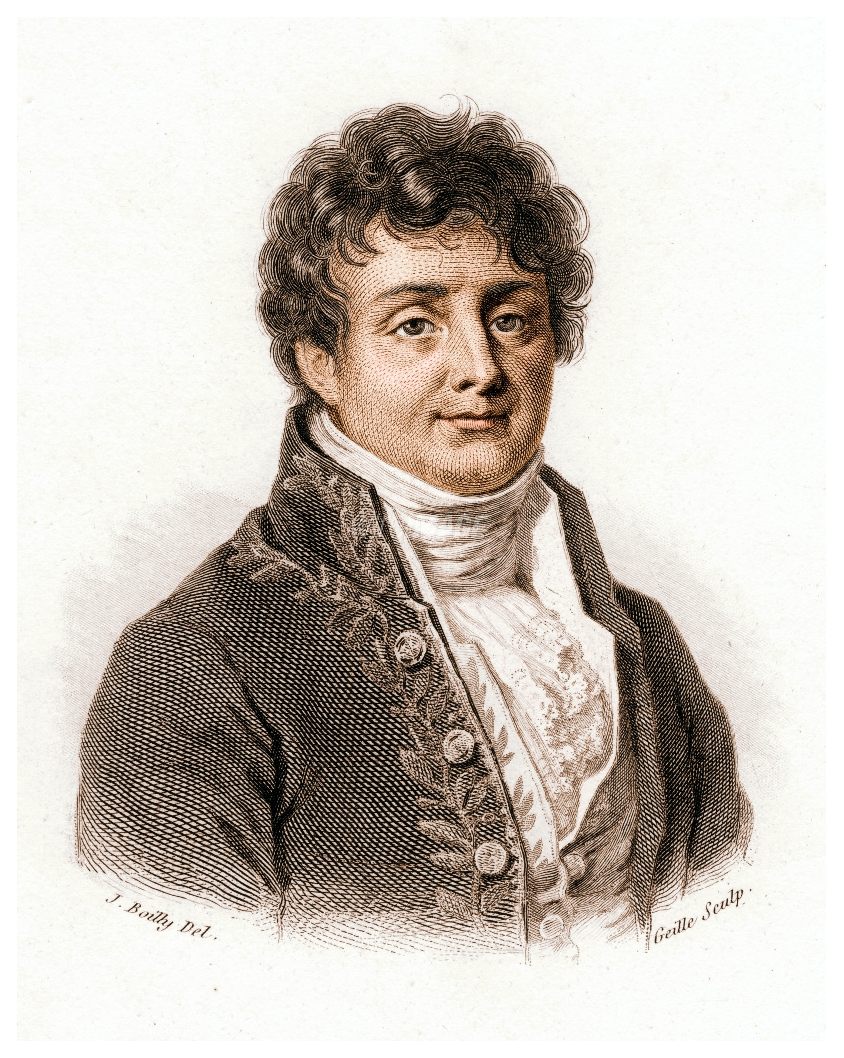
\includegraphics[width=0.9\linewidth]{Fourier}
    \caption*{\index{Fourier, Joseph}\textbf{Jean Baptiste Joseph Fourier}, (1768-1830) mathématicien et physicien 
             français. (Gravure de Julien Léopold Boilly)}
\end{marginfigure}
%-------------------------------------------------------------------------------
%%%%%%%%%%%%%%%%%%%%%%%%%%%%%%%%%%%%%%%%%%%%%%%%%%%%%%%%%%%%%%%%%%%%%%%%%%%%%%%%
%%%%%%%%%%%%%%%%%%%%%%%%%%%%%%%%%%%%%%%%%%%%%%%%%%%%%%%%%%%%%%%%%%%%%%%%%%%%%%%%
\subsection{Définition}
%%%%%%%%%%%%%%%%%%%%%%%%%%%%%%%%%%%%%%%%%%%%%%%%%%%%%%%%%%%%%%%%%%%%%%%%%%%%%%%%
%%%%%%%%%%%%%%%%%%%%%%%%%%%%%%%%%%%%%%%%%%%%%%%%%%%%%%%%%%%%%%%%%%%%%%%%%%%%%%%%
\index{Transformée de Laplace}
La~\gls{tl}, notée $\mathscr{L}$, d'un signal causal $s$ 
fonction d'une variable réelle $t$, est la fonction $S$ 
de la variable complexe $p$, définie par :
%-------------------------------------------------------------------------------
\begin{bequation}[ams align]
S(p)=\laplace{s(t)}=\int_{0}^{+\infty} e^{-pt}s(t)\dd{t}.\label{eq-lap}
\end{bequation}
%-------------------------------------------------------------------------------
On dit également que \textbf{$S(p)$ est l'image dans le domaine de 
Laplace de la fonction $s(t)$ définie dans le domaine temporel.}
Remarquons, dès à présent l'utilisation d'une convention utile: 
\textbf{les fonctions du temps seront toujours désignées par une
minuscule, et les fonctions complexes par la majuscule respective}.
Notons que la transformée de Laplace n'est valide que lorsque la partie réelle 
de p est plus grande qu'une certaine valeur réelle $\alpha$, que l'on nomme 
l'abscisse de convergence avec $-\infty\le\alpha\le+\infty$.

La transformée $S(p)$ de $s(t)$ étant unique, connaissant $S(p)$ on 
en déduit $s(t)$ par la transformation inverse 
\[
    s(t)=\laplacei{S(p)}
\]
Il existe une forme analytique de la transformée inverse basée sur
la formule de Mellin-Fourier\cite{Ostertag}:
\[
    s(t)=\laplacei{S(p)}=\int_{c-j\infty}^{c+j\infty} e^{pt}S(p)\dd{p}
\]
L'intégration de celle-ci est difficile à mettre en oeuvre\footnote{
Il existe différentes méthodes numériques de transformée de Laplace 
inverse (\cref{annexe-invL}). Ces méthodes, hors programme, peuvent 
cependant faire l'objet d'un projet numérique intéressant.}, 
on préferera l'utilisation des tables de transformations de Laplace pour 
réaliser la correspondance inverse (\cref{annexe-lap}). Lorsque la 
transformation n'existe pas dans les tables, il est possible de 
réaliser une décompostion en éléments simples de la réponse $S(p)$ pour 
se placer dans un cas usuel (\cref{annexe-DES}).
\newpage
\restoregeometry
\captionsetup{width=0.9\linewidth,labelfont=bf}
%%%%%%%%%%%%%%%%%%%%%%%%%%%%%%%%%%%%%%%%%%%%%%%%%%%%%%%%%%%%%%%%%%%%%%%%%%%%%%%%
%%%%%%%%%%%%%%%%%%%%%%%%%%%%%%%%%%%%%%%%%%%%%%%%%%%%%%%%%%%%%%%%%%%%%%%%%%%%%%%%
\subsection{Propriétés}
%%%%%%%%%%%%%%%%%%%%%%%%%%%%%%%%%%%%%%%%%%%%%%%%%%%%%%%%%%%%%%%%%%%%%%%%%%%%%%%%
%%%%%%%%%%%%%%%%%%%%%%%%%%%%%%%%%%%%%%%%%%%%%%%%%%%%%%%%%%%%%%%%%%%%%%%%%%%%%%%%
Nous allons ici uniquement présenter les principales propriétés de la TL, 
on se rapportera à nouveau à l'\cref{annexe-lap} pour 
une liste exhaustive de ces propriétés.
%%%%%%%%%%%%%%%%%%%%%%%%%%%%%%%%%%%%%%%%%%%%%%%%%%%%%%%%%%%%%%%%%%%%%%%%%%%%%%%%
\paragraph{Linéarité}
%%%%%%%%%%%%%%%%%%%%%%%%%%%%%%%%%%%%%%%%%%%%%%%%%%%%%%%%%%%%%%%%%%%%%%%%%%%%%%%%
La propriété fondamentale de la transformée de Laplace est d'être linéaire.
Soit deux signaux $s_1(t)$, $s_2(t)$ continus et $S_1(p)$, $S_2(p)$ leurs
transformées de Laplace respectives. La transformée de Laplace d'une 
d'une combinaison linéaire quelconque de $s_1(t)$, $s_2(t)$ est la même 
combinaison linéaire de $S_1(p)$ et $S_2(p)$. Autrement dit,
%-------------------------------------------------------------------------------
\begin{bequation}[ams align]
    \laplace{as_1(t)+bs_2(t)}=aS_1(p)+bS_2(p)
\end{bequation}
%-------------------------------------------------------------------------------
%%%%%%%%%%%%%%%%%%%%%%%%%%%%%%%%%%%%%%%%%%%%%%%%%%%%%%%%%%%%%%%%%%%%%%%%%%%%%%%%
\paragraph{Retard en $t$ (temporel)}
%%%%%%%%%%%%%%%%%%%%%%%%%%%%%%%%%%%%%%%%%%%%%%%%%%%%%%%%%%%%%%%%%%%%%%%%%%%%%%%%
Soit $s(t-\tau)$, un signal $s(t)$ présentant un retard $\tau$.
\[
    \laplace{s(t-\tau)}=\int_{0}^{+\infty} e^{-pt}s(t-\tau)\dd{t}
\]
en appliquant le changement de variable $t'=t-\tau$, on obtient $t=t'+\tau$ 
et $\dd{t}=\dd{t}$
\[
\laplace{s(t-\tau)}
=\int_{\tau}^{+\infty} e^{-p(t'+\tau)}s(t')\dd{t'}
=e^{-p\tau}\int_{0}^{+\infty} e^{-pt'}s(t')\dd{t'}
\]
on reconnaît dans cette dernière expression la définition de la 
transformée de Laplace, on écrit alors :
%-------------------------------------------------------------------------------
\begin{bequation}[ams align]
    \laplace{s(t-\tau)}=e^{-p\tau}S(p)
\end{bequation}
%-------------------------------------------------------------------------------
%%%%%%%%%%%%%%%%%%%%%%%%%%%%%%%%%%%%%%%%%%%%%%%%%%%%%%%%%%%%%%%%%%%%%%%%%%%%%%%%
\paragraph{Retard en $p$ (Thèorème de l'amortissement)}
%%%%%%%%%%%%%%%%%%%%%%%%%%%%%%%%%%%%%%%%%%%%%%%%%%%%%%%%%%%%%%%%%%%%%%%%%%%%%%%%
Soit $s(t)$ un signal de transformée de Laplace $S(p)$. La transformée 
de Laplace du signal modifié $e^{-at}s(t)$ s'écrit :
\[
\laplace{e^{-at}s(t)}
=\int_{0}^{+\infty} e^{-pt}e^{-at}s(t)\dd{t}
=\int_{0}^{+\infty} e^{-(p+a)t}s(t)\dd{t}
\]
on reconnaît dans cette dernière expression la définition de la transformée 
de Laplace pour $p+a$, on obtient donc la transformée, 
%-------------------------------------------------------------------------------
\begin{bequation}[ams align]
    \laplace{e^{-at}s(t)}=S(p+a)
\end{bequation}
%-------------------------------------------------------------------------------
ou encore,
%-------------------------------------------------------------------------------
\begin{bequation}[ams align]
    \laplacei{S(p+a)}=e^{-at}s(t).
\end{bequation}
%-------------------------------------------------------------------------------
%%%%%%%%%%%%%%%%%%%%%%%%%%%%%%%%%%%%%%%%%%%%%%%%%%%%%%%%%%%%%%%%%%%%%%%%%%%%%%%%
\paragraph{Dérivation}
%%%%%%%%%%%%%%%%%%%%%%%%%%%%%%%%%%%%%%%%%%%%%%%%%%%%%%%%%%%%%%%%%%%%%%%%%%%%%%%%
Soit un signal $s(t)$ continu et dérivable pour $t\ge0$ et $S(p)$ 
sa transformée de Laplace. Par définition de la transformée de Laplace 
\[
\laplace{\devi{s(t)}{}}=\int_{0}^{+\infty} e^{-pt}\devi{s(t)}{}\dd{t}
\]
par intégration par parties
%-------------------------------------------------------------------------------
\begin{align*}
    v=e^{-pt}\qquad&\dd{u}=\devi{s(t)}{}\dd{t}\\
    \dd{v}=-pe^{-pt}\dd{t}\qquad&u=s(t)
\end{align*}
%-------------------------------------------------------------------------------
%-------------------------------------------------------------------------------
\begin{align*}
\laplace{\devi{s(t)}{}}&=\left[s(t)e^{-pt}\right]_0
                         ^{+\infty}-p\int_{0}^{+\infty}e^{-pt}s(t)\dd{t}\\
                         &=-s(0)+pS(p)
\end{align*}
%-------------------------------------------------------------------------------
ou encore
%-------------------------------------------------------------------------------
\begin{bequation}[ams align]
    \laplace{\devi{s(t)}{}}=pS(p)-s(0)
\end{bequation}
%-------------------------------------------------------------------------------
On généralise à tous les ordres de dérivation dans le cas de conditions 
initiales nulles.
\[
\laplace{\devi{s(t)}{n}}=p^nS(p)
\]
Remarquons alors que \textbf{dériver dans le domaine temporel consiste 
à multiplier par $p$ dans le domaine de Laplace.}
%%%%%%%%%%%%%%%%%%%%%%%%%%%%%%%%%%%%%%%%%%%%%%%%%%%%%%%%%%%%%%%%%%%%%%%%%%%%%%%%
\paragraph{Intégration}
%%%%%%%%%%%%%%%%%%%%%%%%%%%%%%%%%%%%%%%%%%%%%%%%%%%%%%%%%%%%%%%%%%%%%%%%%%%%%%%%
Soient  des signaux $v(t)$ et $s(t)$ tel que 
$v(t)=\int_{0}^{t}s(\tau)\dd{\tau}$. Par définition,
\[
\laplace{v(t)}=\int_{0}^{+\infty} e^{-pt}v(t)\dd{t}
\]
par intégration par parties,
%-------------------------------------------------------------------------------
\begin{align*}
    v=v(t)\qquad&\dd{u}=e^{-pt}\dd{t}\\
    \dd{v}=s(t)\dd{t}\qquad&u=-\dfrac{1}{p}e^{-pt}
\end{align*} 
%-------------------------------------------------------------------------------
\begin{align*}
    \laplace{v(t)}&=\left[-\dfrac{1}{p}v(t)e^{-pt}\right]_0^{+\infty}
                          -\int_{0}^{+\infty}
                          -\dfrac{1}{p}e^{-pt}s(t)\dd{t} \\
    &=\dfrac{1}{p}\int_{0}^{+\infty} e^{-pt}s(t)\dd{t}+\dfrac{s(0)}{p}
\end{align*}
%-------------------------------------------------------------------------------
ou encore
%-------------------------------------------------------------------------------
\begin{bequation}[ams align]
    \laplace{\int_{0}^{t}s(\tau)\dd{\tau}}=\dfrac{S(p)}{p}+\dfrac{s(0)}{p}
\end{bequation}
%-------------------------------------------------------------------------------
Remarquons alors que \textbf{intégrer dans le domaine temporel consiste à 
diviser par $p$ dans le domaine de Laplace.}
%%%%%%%%%%%%%%%%%%%%%%%%%%%%%%%%%%%%%%%%%%%%%%%%%%%%%%%%%%%%%%%%%%%%%%%%%%%%%%%%
\paragraph{Théorème de la valeur initiale}
%%%%%%%%%%%%%%%%%%%%%%%%%%%%%%%%%%%%%%%%%%%%%%%%%%%%%%%%%%%%%%%%%%%%%%%%%%%%%%%%
\index{Théorème!de la valeur initiale}
%-------------------------------------------------------------------------------
\begin{bequation}[ams align]
    s(0)=\lim\limits_{p\rightarrow+\infty} p S(p)\qquad \forall S(p)
\end{bequation}
%-------------------------------------------------------------------------------
où $s(0)$ est la valeur d'un signal $s(t)$ pour $t=0$.
Ce théorème est utilisé pour déterminer la valeur initiale
dans le domaine temporelle d'un signal dont on connait 
uniquement la transformée de Laplace.
%%%%%%%%%%%%%%%%%%%%%%%%%%%%%%%%%%%%%%%%%%%%%%%%%%%%%%%%%%%%%%%%%%%%%%%%%%%%%%%%
\paragraph{Théorème de la valeur finale}
%%%%%%%%%%%%%%%%%%%%%%%%%%%%%%%%%%%%%%%%%%%%%%%%%%%%%%%%%%%%%%%%%%%%%%%%%%%%%%%%
\index{Théorème!de la valeur finale}
%-------------------------------------------------------------------------------
\begin{bequation}[ams align]
    s(\infty)=\lim\limits_{p\rightarrow0} p S(p)
\end{bequation}
%-------------------------------------------------------------------------------
où $s(\infty)$ est la valeur d'un signal $s(t)$ pour $t\to\infty$.
Ce théorème n'est valable que si $s(\infty)$ est définie. Ou comme on le 
dira plus tard si le signal est stable.
%%%%%%%%%%%%%%%%%%%%%%%%%%%%%%%%%%%%%%%%%%%%%%%%%%%%%%%%%%%%%%%%%%%%%%%%%%%%%%%%
\paragraph{Transformée de Laplace d'un produit de convolution}
%%%%%%%%%%%%%%%%%%%%%%%%%%%%%%%%%%%%%%%%%%%%%%%%%%%%%%%%%%%%%%%%%%%%%%%%%%%%%%%%
Le produit de convolution de deux signaux $h(t)$ et $e(t)$ que l'on 
note $(h*e)(t)$ est défini par :
\[
    (h*e)(t)=\int_{-\infty}^{+\infty}h(t-\tau)e(\tau)\dd{\tau}
\]
La transformée de Laplace transforme le produit de convolution en un simple
produit des signaux dans le domaine de Laplace. Formellement,
%-------------------------------------------------------------------------------
\begin{bequation}[ams align]
    \laplace{(h*e)(t)}=H(p)E(p)
\end{bequation}
%-------------------------------------------------------------------------------
Si cette propriété est fondamentale, nous ne l'utiliserons 
que très exceptionnellement. Nous la rencontrerons à nouveau, 
dans ce chapitre, lorsque nous introduierons la fonction de 
transfert d'un système linéaire.
%%%%%%%%%%%%%%%%%%%%%%%%%%%%%%%%%%%%%%%%%%%%%%%%%%%%%%%%%%%%%%%%%%%%%%%%%%%%%%%%
%%%%%%%%%%%%%%%%%%%%%%%%%%%%%%%%%%%%%%%%%%%%%%%%%%%%%%%%%%%%%%%%%%%%%%%%%%%%%%%%
\subsection{Transformées des signaux usuels}
%%%%%%%%%%%%%%%%%%%%%%%%%%%%%%%%%%%%%%%%%%%%%%%%%%%%%%%%%%%%%%%%%%%%%%%%%%%%%%%%
%%%%%%%%%%%%%%%%%%%%%%%%%%%%%%%%%%%%%%%%%%%%%%%%%%%%%%%%%%%%%%%%%%%%%%%%%%%%%%%%
Nous présentons les transformées de Laplace des signaux usuels introduits
au paragraphe~\ref{sec-signaux_usuels}
%%%%%%%%%%%%%%%%%%%%%%%%%%%%%%%%%%%%%%%%%%%%%%%%%%%%%%%%%%%%%%%%%%%%%%%%%%%%%%%%
\paragraph{Transformée d'une impulsion de Dirac}
%%%%%%%%%%%%%%%%%%%%%%%%%%%%%%%%%%%%%%%%%%%%%%%%%%%%%%%%%%%%%%%%%%%%%%%%%%%%%%%%
\index{Transformée de Laplace!d'une impulsion de Dirac}
Par simple application des définitions 
de la~\gls{tl} et de l'impulsion de Dirac, la transformée d'une 
impulsion de Dirac $\delta(t)$ s'écrit:
\[
    \laplace{\delta(t)}=\int_{0}^{+\infty} e^{-pt}\,\delta(t)\dd{t}=1
\]
ou encore
%-------------------------------------------------------------------------------
\begin{bequation}[ams align]
    \laplace{\delta(t)}=1
\end{bequation}
%-------------------------------------------------------------------------------
%%%%%%%%%%%%%%%%%%%%%%%%%%%%%%%%%%%%%%%%%%%%%%%%%%%%%%%%%%%%%%%%%%%%%%%%%%%%%%%%
\paragraph{Transformée d'un échelon-unité}
%%%%%%%%%%%%%%%%%%%%%%%%%%%%%%%%%%%%%%%%%%%%%%%%%%%%%%%%%%%%%%%%%%%%%%%%%%%%%%%%
\index{Transformée de Laplace!d'un échelon-unité}
La transformée de Laplace d'un signal échelon-unité  s'écrit : 
\[
\laplace{u(t)}=\int_{0}^{+\infty}e^{-pt}\,u(t)\dd{t}
=\int_{0}^{+\infty} e^{-pt}\dd{t}
=\left[\dfrac{-e^{-pt}}{p}\right]_0^{+\infty}=\dfrac{1}{p}
\]
ou encore
%-------------------------------------------------------------------------------
\begin{bequation}[ams align]
    \laplace{u(t)}=\dfrac{1}{p}
\end{bequation}
%-------------------------------------------------------------------------------
Dans le cas de la forme généralisée, il suffit de multiplier par une constante.
%%%%%%%%%%%%%%%%%%%%%%%%%%%%%%%%%%%%%%%%%%%%%%%%%%%%%%%%%%%%%%%%%%%%%%%%%%%%%%%%
\paragraph{Transformée d'une rampe}
%%%%%%%%%%%%%%%%%%%%%%%%%%%%%%%%%%%%%%%%%%%%%%%%%%%%%%%%%%%%%%%%%%%%%%%%%%%%%%%%
\index{Transformée de Laplace!d'une rampe}
La transformée de Laplace d'un signal rampe s'écrit :
\[
\laplace{r(t)}=\int_{0}^{+\infty} e^{-pt}r(t)\dd{t}
=\int_{0}^{+\infty} te^{-pt}\dd{t}
\]
Par intégration par parties:
%-------------------------------------------------------------------------------
\begin{align*}
    v=-\dfrac{1}{p}e^{-pt}\qquad&\dd{u}=\dd{t}\\
    \dd{v}=e^{-pt}\dd{t}\qquad&u=t
\end{align*}
%-------------------------------------------------------------------------------
\[
\int_{0}^{+\infty} te^{-pt}\dd{t}
=\left[-t\dfrac{1}{p}e^{-pt}\right]_0^{+\infty}-\int_{0}^{+\infty}
-\dfrac{1}{p}e^{-pt}\dd{t}=\dfrac{1}{p^2}
\]
ou encore
%-------------------------------------------------------------------------------
\begin{bequation}[ams align]
    \laplace{r(t)}=\laplace{t\cdot u(t)}=\dfrac{1}{p^2}.
\end{bequation}
%-------------------------------------------------------------------------------
On généralise aux ordres supérieures (\og parabolique\fg, \og 
cubique\fg\ldots) :
%-------------------------------------------------------------------------------
\begin{bequation}[ams align]
    \laplace{\dfrac{1}{n!}t^n\cdot u(t)}=\dfrac{1}{p^{n+1}}.
\end{bequation}
%-------------------------------------------------------------------------------
%%%%%%%%%%%%%%%%%%%%%%%%%%%%%%%%%%%%%%%%%%%%%%%%%%%%%%%%%%%%%%%%%%%%%%%%%%%%%%%%
\paragraph{Transformée d'une exponentielle décroissante}
%%%%%%%%%%%%%%%%%%%%%%%%%%%%%%%%%%%%%%%%%%%%%%%%%%%%%%%%%%%%%%%%%%%%%%%%%%%%%%%%
\index{Transformée de Laplace!d'une exponentielle décroissante}
La transformée de Laplace d'une exponentielle décroissante s'écrit :
\[
\laplace{e^{-at}u(t)}=\int_{0}^{+\infty} e^{-pt}e^{-at}\dd{t}
=\int_{0}^{+\infty} e^{-(p+a)t}\dd{t} = \dfrac{1}{p+a}
\]
ou encore
%-------------------------------------------------------------------------------
\begin{bequation}[ams align]
    \laplace{e^{-at}u(t)}=\dfrac{1}{p+a}
\end{bequation}
%-------------------------------------------------------------------------------
Nous aurions pu utiliser la propriété du retard en $p$ 
(Théorème de l'amortissement) pour déterminer cette transformée de Laplace.
%%%%%%%%%%%%%%%%%%%%%%%%%%%%%%%%%%%%%%%%%%%%%%%%%%%%%%%%%%%%%%%%%%%%%%%%%%%%%%%%
\paragraph{Transformée d'un sinus}
%%%%%%%%%%%%%%%%%%%%%%%%%%%%%%%%%%%%%%%%%%%%%%%%%%%%%%%%%%%%%%%%%%%%%%%%%%%%%%%%
\index{Transformée de Laplace!d'un sinus}
La transformée de Laplace de la fonction sinus s'écrit :
%-------------------------------------------------------------------------------
\begin{align*}
\laplace{\sin{\omega t}\cdot u(t)}&=
\int_{0}^{+\infty}e^{-pt}\dfrac{e^{\jw t}-e^{-\jw t}}{2j}\dd{t}\\
&=\dfrac{1}{2j}\int_{0}^{+\infty}e^{-(p-\jw)t}\dd{t} - 
  \dfrac{1}{2j}\int_{0}^{+\infty}e^{-(p+\jw)t}\dd{t} \\
&=\dfrac{1}{2j}\left( \dfrac{1}{p-\jw}-\dfrac{1}{p+\jw}\right)\\
&=\dfrac{\omega}{p^2+\omega^2}
\end{align*}
%-------------------------------------------------------------------------------
ou encore
%-------------------------------------------------------------------------------
\begin{bequation}[ams align]
    \laplace{\sin{\omega t}\cdot u(t)}=\dfrac{\omega}{p^2+\omega^2}
\end{bequation}
%-------------------------------------------------------------------------------
%%%%%%%%%%%%%%%%%%%%%%%%%%%%%%%%%%%%%%%%%%%%%%%%%%%%%%%%%%%%%%%%%%%%%%%%%%%%%%%%
\paragraph{Transformée d'un cosinus}
%%%%%%%%%%%%%%%%%%%%%%%%%%%%%%%%%%%%%%%%%%%%%%%%%%%%%%%%%%%%%%%%%%%%%%%%%%%%%%%%
\index{Transformée de Laplace!d'un cosinus}
La transformée de Laplace de la fonction cosinus s'écrit :
%-------------------------------------------------------------------------------
\begin{align*}
\laplace{\cos{\omega t}\cdot u(t)}&=\int_{0}^{+\infty}e^{-pt}
\dfrac{e^{\jw t}+e^{-\jw t}}{2}\dd{t}\\
&=\dfrac{1}{2}\int_{0}^{+\infty}e^{-(p-\jw)t}\dd{t} + 
\dfrac{1}{2j}\int_{0}^{+\infty}e^{-(p+\jw)t}\dd{t} \\
&=\dfrac{1}{2}\left( \dfrac{1}{p-\jw}+\dfrac{1}{p+\jw}\right)\\
&=\dfrac{p}{p^2+\omega^2}
\end{align*}
%-------------------------------------------------------------------------------
ou encore
%-------------------------------------------------------------------------------
\begin{bequation}[ams align]
    \laplace{\cos{\omega t}\cdot u(t)}=\dfrac{p}{p^2+\omega^2}
\end{bequation}
%-------------------------------------------------------------------------------
\newpage
\input{re/newgeometry}
\captionsetup{width=0.9\linewidth,labelfont=bf}
%%%%%%%%%%%%%%%%%%%%%%%%%%%%%%%%%%%%%%%%%%%%%%%%%%%%%%%%%%%%%%%%%%%%%%%%%%%%%%%%
%%%%%%%%%%%%%%%%%%%%%%%%%%%%%%%%%%%%%%%%%%%%%%%%%%%%%%%%%%%%%%%%%%%%%%%%%%%%%%%%
\subsection[Application de la transformée de Laplace]
           {Application de la TL à la résolution d'équation différentielle}
%%%%%%%%%%%%%%%%%%%%%%%%%%%%%%%%%%%%%%%%%%%%%%%%%%%%%%%%%%%%%%%%%%%%%%%%%%%%%%%%
%%%%%%%%%%%%%%%%%%%%%%%%%%%%%%%%%%%%%%%%%%%%%%%%%%%%%%%%%%%%%%%%%%%%%%%%%%%%%%%%
%-------------------------------------------------------------------------------
\begin{figure}[!ht]
    \centering
    \tikzsetnextfilename{laplace_schema-chap_slci-ext}
    \begin{tikzpicture}
\tikzset{both/.style={draw,minimum width=4cm,minimum height=2cm,rounded corners=.1cm,inner sep=0.5pt,text width=4cm,align=center}}
\tikzstyle{temp}=[both,fill=blue!25!white]
\tikzstyle{lapl}=[both,fill=red!25!white]
\node[temp] (a) at (0,0)  {\small\'Equation différentielle\\ (domaine temporel)};
\node[temp] (b) at (7,0)  {\small Solution \\(domaine temporel)};
\node[lapl] (c) at  (0,-4){\small \'Equation algébrique\\ (domaine de Laplace)};
\node[lapl] (d) at (7,-4) {\small Solution \\(domaine de Laplace)};
\draw[very thick,-{Latex[length=3.5mm]}] (a) --node[above,align=center,text width=2cm] {Résolution\\direct} (b);
\draw[very thick,-{Latex[length=3.5mm]}] (d) --node[right] {\Large$\mathscr{L}^{-1}$} (b);
\draw[very thick,-{Latex[length=3.5mm]}] (a) --node[left] {\Large$\mathscr{L}$} (c);
\draw[very thick,-{Latex[length=3.5mm]}] (c) --node[below,align=center,text width=2cm] {Résolution\\algébrique} (d);
\end{tikzpicture}



    \caption{Représentation schématique de la méthode employée pour la 
             résolution des équations différentielles linéaires à 
             coefficients constants.\label{fig-laplace_schema}}
\end{figure}
%-------------------------------------------------------------------------------
%%%%%%%%%%%%%%%%%%%%%%%%%%%%%%%%%%%%%%%%%%%%%%%%%%%%%%%%%%%%%%%%%%%%%%%%%%%%%%%%
\subsubsection{Méthodologie}
%%%%%%%%%%%%%%%%%%%%%%%%%%%%%%%%%%%%%%%%%%%%%%%%%%%%%%%%%%%%%%%%%%%%%%%%%%%%%%%%
Lorsqu'une équation différentielle à coefficients constants a pu être établie
pour définir la relation entre l'entrée et la sortie d'un \gls{slci}, il 
nous faut en trouver une solution. Les méthodes classiques de résolution 
d'équations différentielles peuvent être difficiles et fastidieuses à mettre 
en oeuvre, notamment dans le cas d'équation différentielle d'ordre élevé 
ou encore pour des systèmes composés de sous-systèmes.

La transformée de Laplace permet de mettre en oeuvre une méthode plus simple et 
systèmatique  pour la la résolution de ces équations différentielles à 
coefficients constants.

Comme nous l'avons déjà discuté, la forme générale de ces équations est 
donnée par :
%-------------------------------------------------------------------------------
\begin{align}
    \sum_{i=0}^{n}a_i\devi{s(t)}{i}=\sum_{i=0}^{m}b_i\devi{e(t)}{i}
    \label{eq-ltemp}
\end{align}
%-------------------------------------------------------------------------------
avec $n,m\in\mathbb{N}$, $s(t)$ le signal de sortie, $e(t)$ le signal 
d'entrée et $a_i,b_i\in\mathbb{R}$. L'équation est dite d'ordre $n$.
%-------------------------------------------------------------------------------
\begin{marginfigure}
    \centering
    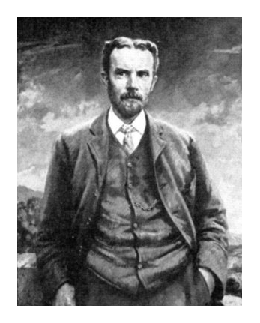
\includegraphics[width=0.9\linewidth]{OliverHeaviside.eps}
    \caption*{\index{Heaviside, Oliver}\textbf{Oliver Heaviside} (1850-1925), 
              physicien britannique. Il développa le calcul opérationnel 
              pour résoudre les équations différentielles}.
\end{marginfigure}
%-------------------------------------------------------------------------------
Sous cette forme, cette équation différentielle constitue ce que l'on 
nomme \textbf{la loi temporelle} du système. Sans perte de généralité, on ne 
considèrera dans un premier temps que les systèmes pour lesquels toutes les 
\textbf{conditions initialles sont nulles}, appelées également les conditions 
d'Heaviside
\newpage
\restoregeometry
\captionsetup{width=0.9\linewidth,labelfont=bf}
En appliquant la transformée de Laplace à l'\cref{eq-ltemp}, on obtient 
ce que l'on nomme \textbf{la loi fréquentielle} du système :
%-------------------------------------------------------------------------------
\begin{bequation}[ams align]
    \sum_{i=0}^{n}a_ip^iS(p)=\sum_{i=0}^{m}b_ip^iE(p)\label{eq-lfreq}
\end{bequation}
%-------------------------------------------------------------------------------
La résolution algébrique de cette équation est simplement donnée par :
%-------------------------------------------------------------------------------
\begin{bequation}[ams align]
    S(p)=\dfrac{\sum\limits_{i=0}^{m}b_ip^i}
    {\sum\limits_{i=0}^{n}a_ip^i}E(p)\label{eq-lfreq2}
\end{bequation}
%-------------------------------------------------------------------------------
La solution dans le domaine temporelle $s(t)$ de l'équation différentielle 
est alors simplement obtenue par transformée de Laplace inverse de $S(p)$.

Cette méthode, résumée par l'organigramme de la~\cref{fig-laplace_schema}, 
est appliqué à un exemple complet au paragraphe suivant.
%%%%%%%%%%%%%%%%%%%%%%%%%%%%%%%%%%%%%%%%%%%%%%%%%%%%%%%%%%%%%%%%%%%%%%%%%%%%%%%%
\subsubsection{Exemple complet}
%%%%%%%%%%%%%%%%%%%%%%%%%%%%%%%%%%%%%%%%%%%%%%%%%%%%%%%%%%%%%%%%%%%%%%%%%%%%%%%%
Soit l'équation différentielle suivante :
%-------------------------------------------------------------------------------
\begin{align}
\devi{s(t)}{2}+2\devi{s(t)}{} + s(t) = e(t)\label{eq-diff1}
\end{align}
%-------------------------------------------------------------------------------
où $e(t)$ et $s(t)$ sont respectivement les fonctions temporelles de l'entrée 
et de la sortie du système régi par cette équation différentielle. 
Nous considérons la réponse à un échelon-unité (c.-à-d. $e(t)=u(t)$ ) 
avec pour conditions initiales :
%-------------------------------------------------------------------------------
\begin{align*}
    s(0) &=-1\\
    s'(0)&=2.
\end{align*}
%-------------------------------------------------------------------------------
Nous allons résoudre cette équation par deux méthodes différentes: 
\textbf{la méthode direct de résolution d'équations différentielles avec 
second membre}, et par l'\textbf{application de la transformée de Laplace}.
Nous pourrons observer que l'application de la TL pour la résolution
des équations différentielles est une méthode plus systèmatique qui 
s'affranchit de la forme particulière de l'équation différentielle 
auquelle on a à faire. Nous verrons que la transformée de Laplace devient 
totalement indispensable pour la caractérisation d'un \gls{slci}.
\newpage
\input{re/newgeometry}
\captionsetup{width=0.9\linewidth,labelfont=bf}
%%%%%%%%%%%%%%%%%%%%%%%%%%%%%%%%%%%%%%%%%%%%%%%%%%%%%%%%%%%%%%%%%%%%%%%%%%%%%%%%
\paragraph{Résolution par la méthode direct}
%%%%%%%%%%%%%%%%%%%%%%%%%%%%%%%%%%%%%%%%%%%%%%%%%%%%%%%%%%%%%%%%%%%%%%%%%%%%%%%%
L'équation caractéristique associée à cette équation différentielle est 
donnée par 
\[
    r^2+2r+1=0
\]
cette équation possède une solution double $r_{1,2}=-1$.
La solution générale de l'équation homogène $s_0(t)$ (c.a.d sans second membre) 
est donc de la forme :
\[
    s_0(t)=(\alpha t+\beta)e^{-t}.
\]
Une solution particulière $s_1(t)=1$ nous est trivialement donnée par l'entrée 
en échelon qui correspond au régime permanent.
La solution générale est donc donnée par :
\[
    s(t)=(\alpha t+\beta)e^{-t}+1
\]
Dérivons cette solution générale pour pouvoir déterminer les coefficients 
$\alpha$, $\beta$ en utilisant les conditions initiales,
%-------------------------------------------------------------------------------
\begin{align*}
    s'(t)&=\alpha e^{-t}-(\alpha t+\beta)e^{-t}\\
     s(0)&=-1\Rightarrow\beta+1=-1\Rightarrow\beta=-2 \\
    s'(0)&=\hphantom{-}2\Rightarrow\alpha+2=\hphantom{-}2\Rightarrow\alpha=0
\end{align*}
%-------------------------------------------------------------------------------
La solution générale de l'équation différentielle~(\ref{eq-diff1}) est 
donc donnée par 
%-------------------------------------------------------------------------------
\begin{marginfigure}
    \centering
    \tikzsetnextfilename{sol_eq_diff-chap_slci-ext}
    \resizebox{\linewidth}{!}{\input{tikz/sol_eq_diff-chap_slci.tex}}
    \caption{Représentation de la solution générale de l'équation 
             différentielle~(\ref{eq-diff1}) pour $e(t)=u(t)$. 
             On vérifie lors du tracé que l'on observe bien les principales 
             propriétes du signal (c.-à-d. conditions initiales, 
             valeur finale).\label{fig-solution}}
\end{marginfigure}
%-------------------------------------------------------------------------------
%-------------------------------------------------------------------------------
\begin{bequation}[ams align]
s(t)=1-2e^{-t}.
\end{bequation}
%-------------------------------------------------------------------------------
Nous laissons au lecteur le soin de vérifier que cette fonction est solution 
de l'équation~\ref{eq-diff1}, et qu'elle respecte notamment les conditions 
initiales. Le graphe de la solution est également présenté 
(\Cref{fig-solution}).
%%%%%%%%%%%%%%%%%%%%%%%%%%%%%%%%%%%%%%%%%%%%%%%%%%%%%%%%%%%%%%%%%%%%%%%%%%%%%%%%
\paragraph{Résolution par application de la transformée de Laplace}
%%%%%%%%%%%%%%%%%%%%%%%%%%%%%%%%%%%%%%%%%%%%%%%%%%%%%%%%%%%%%%%%%%%%%%%%%%%%%%%%
\index{Transformée de Laplace! résolution d'équation différentielle}
La transformée de Laplace est linéaire. Il nous est alors possible
de l'appliquer aux différents termes de l'équation 
différentielle~(\ref{eq-diff1}) séparément.
On obtient pour chacun des termes :
%-------------------------------------------------------------------------------
\begin{align*}
    \laplace{s(t)} &= S(p), \\
    \laplace{\devi{s(t)}{}} &= pS(p)-s(0) = pS(p) +1, \\
    \laplace{\devi{s(t)}{2}} &= p^2S(p)-ps(0)-s'(0) = p^2S(p) + p -2,\\
    \laplace{u(t)} &= \dfrac{1}{p}.
\end{align*}
%-------------------------------------------------------------------------------
\newpage
\restoregeometry
\captionsetup{width=0.9\linewidth,labelfont=bf}
L'équation différentielle~(\ref{eq-diff1}) devient dans le domaine 
de Laplace :
%-------------------------------------------------------------------------------
\begin{align*}
p^2S(p)+p-2+2pS(p)+2+S(p)=\dfrac{1}{p} 
\end{align*}
%-------------------------------------------------------------------------------
En réarrangeant cette expression, il est possible de déterminer la 
forme de la réponse $S(p)$ dans le domaine de Laplace.
%-------------------------------------------------------------------------------
\begin{align*}
    S(p)\left(p^2+2p+1\right)+p&=\dfrac{1}{p} \\
    %S(p)\left(p+1\right)^2 &= \dfrac{1-p^2}{p}\\
    S(p)&= \dfrac{1-p^2}{p\left(p+1\right)^2}
\end{align*}
%-------------------------------------------------------------------------------
de Laplace usuels, nous allons décomposer cette
fraction rationnelle en éléments simples (\Cref{annexe-DES}).
\[
    S(p)=\dfrac{A}{p}+\dfrac{B}{p+1}+\dfrac{C}{(p+1)^2}
\]
Par identification, 
\[
    S(p)=\dfrac{A(p+1)^2+Bp(p+1)+Cp}{p(p+1)^2}
        =\dfrac{1-p^2}{p\left(p+1\right)^2}
\]
\[
\begin{cases}
    A+B&=-1 \\
    2A+B+C&=0 \\
    A&=1   
\end{cases}\Rightarrow
\begin{cases}
    B&=-2\\
    C&=0
\end{cases}
\]
La réponse $S(p)$ se décompose donc de la façon suivante en éléments simples:
\[
    S(p)=\dfrac{1}{p}-\dfrac{2}{p+1}
\]
Il est maintenant plus aisé d'appliquer la transformation de Laplace inverse, 
en utilisant le tableau des transformées de Laplace usuels 
(c.f lignes 3 et 7 du tableau de l'\Cref{annexe-lap}) pour obtenir la 
réponse temporelle $s(t)$. Notamment,
\[
    \laplacei{\dfrac{1}{p}}=1
\]
et
\[
    \laplacei{\dfrac{2}{p+1}}=2e^{-t}
\]
soit 
%-------------------------------------------------------------------------------
\begin{bequation}[ams align]
    \laplacei{S(p)}=s(t)=1-2e^{-t}
\end{bequation}
%-------------------------------------------------------------------------------
Comme attendu, les deux méthodes donnent le même résultat, cependant 
la transformée de Laplace permet de définir dans le domaine de Laplace, une 
relation direct entre l'entrée et la sortie d'un système. C'est la fonction 
de transfert qui réalise ce lien.
\clearpage
%%%%%%%%%%%%%%%%%%%%%%%%%%%%%%%%%%%%%%%%%%%%%%%%%%%%%%%%%%%%%%%%%%%%%%%%%%%%%%%%
%%%%%%%%%%%%%%%%%%%%%%%%%%%%%%%%%%%%%%%%%%%%%%%%%%%%%%%%%%%%%%%%%%%%%%%%%%%%%%%%
%%%%%%%%%%%%%%%%%%%%%%%%%%%%%%%%%%%%%%%%%%%%%%%%%%%%%%%%%%%%%%%%%%%%%%%%%%%%%%%%
\section{Fonction de Transfert}
%%%%%%%%%%%%%%%%%%%%%%%%%%%%%%%%%%%%%%%%%%%%%%%%%%%%%%%%%%%%%%%%%%%%%%%%%%%%%%%%
%%%%%%%%%%%%%%%%%%%%%%%%%%%%%%%%%%%%%%%%%%%%%%%%%%%%%%%%%%%%%%%%%%%%%%%%%%%%%%%%
%%%%%%%%%%%%%%%%%%%%%%%%%%%%%%%%%%%%%%%%%%%%%%%%%%%%%%%%%%%%%%%%%%%%%%%%%%%%%%%%
%%%%%%%%%%%%%%%%%%%%%%%%%%%%%%%%%%%%%%%%%%%%%%%%%%%%%%%%%%%%%%%%%%%%%%%%%%%%%%%%
%%%%%%%%%%%%%%%%%%%%%%%%%%%%%%%%%%%%%%%%%%%%%%%%%%%%%%%%%%%%%%%%%%%%%%%%%%%%%%%%
\subsection{Définition}
%%%%%%%%%%%%%%%%%%%%%%%%%%%%%%%%%%%%%%%%%%%%%%%%%%%%%%%%%%%%%%%%%%%%%%%%%%%%%%%%
%%%%%%%%%%%%%%%%%%%%%%%%%%%%%%%%%%%%%%%%%%%%%%%%%%%%%%%%%%%%%%%%%%%%%%%%%%%%%%%%
\index{Fonction de Transfert}
La fonction de transfert $H(p)$ d'un système est donnée par le rapport de la 
sortie $S(p)$ et l'entrée $E(p)$ dans le domaine de Laplace. 
%-------------------------------------------------------------------------------
\begin{bequation}[ams align]
    H(p)=\dfrac{S(p)}{E(p)}
\end{bequation}
%-------------------------------------------------------------------------------
ou encore,
%-------------------------------------------------------------------------------
\begin{bequation}[ams align]
    S(p)=H(p)E(p)\label{eq-she}
\end{bequation}
%-------------------------------------------------------------------------------
Cette fonction $H(p)$, également appelé \textbf{transmittance}, caractérise 
le système de façon univoque. Pour une entrée donnée il est possible de 
prévoir la sortie d'un système caractérisé par sa fonction de transfert $H(p)$.

Nous représenterons très souvent cette relation dans le domaine de Laplace 
par le schéma-bloc suivant : 
%-------------------------------------------------------------------------------
\begin{center}
    \tikzsetnextfilename{sb_bloc_FT-chap_slci-ext}
    \begin{tikzpicture}
    \sbEntree{E1}
    \sbBloc[3]{B1}{$H(p)$}{E1}
    \sbRelier[$E(p)$]{E1}{B1}
    \sbSortie[3]{S1}{B1}
    \sbRelier[$S(p)$]{B1}{S1}
\end{tikzpicture}

\end{center}
%-------------------------------------------------------------------------------
%Cette relation entre la sortie et l'entrée du système dans le domaine de 
%Laplace provient directement de la relation temporelle associée à l'équation 
%différentielle du phénomène physique mis en jeu.
%%%%%%%%%%%%%%%%%%%%%%%%%%%%%%%%%%%%%%%%%%%%%%%%%%%%%%%%%%%%%%%%%%%%%%%%%%%%%%%%
%%%%%%%%%%%%%%%%%%%%%%%%%%%%%%%%%%%%%%%%%%%%%%%%%%%%%%%%%%%%%%%%%%%%%%%%%%%%%%%%
\subsection{Lien entre fonction de transfert et réponse impulsionnelle}
%%%%%%%%%%%%%%%%%%%%%%%%%%%%%%%%%%%%%%%%%%%%%%%%%%%%%%%%%%%%%%%%%%%%%%%%%%%%%%%%
%%%%%%%%%%%%%%%%%%%%%%%%%%%%%%%%%%%%%%%%%%%%%%%%%%%%%%%%%%%%%%%%%%%%%%%%%%%%%%%%
À partir de l'équation~\ref{eq-she}, le lien entre la fonction de transfert
et la réponse impulsionnelle paraît évident. En effet, pour une impulsion 
de Dirac en entrée, la réponse impulsionnelle est simplement donnée par 
la fonction de transfert puisque $\laplace{\delta(t)}=E(p)=1$. 
Autrement dit, la fonction de transfert d'un système est la 
réponse impulsionnelle dans le domaine de Laplace. Ou encore, si $h(t)$ 
est la réponse impulsionnelle d'un système alors,
\[
    H(p) = \laplace{h(t)}
\]
D'après la propriété du produit de convolution, nous savons que 
le produit de deux fonctions dans le domaine de Laplace correspond au 
produit de convolution de ces deux fonctions dans le domaine temporelle, 
dans le cas de l'équation~\ref{eq-she},
\[
    s(t)=\laplacei{S(p)}=\laplacei{H(p)E(p)}
    =\int_{-\infty}^{+\infty}h(t-\tau)e(\tau)\dd{\tau}
\]
%\newpage
ou encore,
%-------------------------------------------------------------------------------
\begin{bequation}[ams align]
    s(t)=(h*e)(t)
\end{bequation}
%-------------------------------------------------------------------------------
Cette dernière exprime que \textbf{la réponse, dans le domaine temporel, 
d'un système est donnée par le 
produit de convolution de l'entrée $e(t)$ et la réponse impulsionnelle $h(t)$.}
%%%%%%%%%%%%%%%%%%%%%%%%%%%%%%%%%%%%%%%%%%%%%%%%%%%%%%%%%%%%%%%%%%%%%%%%%%%%%%%%
%%%%%%%%%%%%%%%%%%%%%%%%%%%%%%%%%%%%%%%%%%%%%%%%%%%%%%%%%%%%%%%%%%%%%%%%%%%%%%%%
\subsection
[Représentation de la fonction de transfert]
{Représentations algébrique et graphique de la fonction de transfert}
%%%%%%%%%%%%%%%%%%%%%%%%%%%%%%%%%%%%%%%%%%%%%%%%%%%%%%%%%%%%%%%%%%%%%%%%%%%%%%%%
%%%%%%%%%%%%%%%%%%%%%%%%%%%%%%%%%%%%%%%%%%%%%%%%%%%%%%%%%%%%%%%%%%%%%%%%%%%%%%%%
D'après la loi fréquentielle (\Cref{eq-lfreq}), la fonction de transfert 
d'un \gls{slci}~peut s'écrire sous la forme d'une fraction rationnelle,
%-------------------------------------------------------------------------------
\begin{bequation}[ams align]
H(p)=\dfrac{\sum\limits_{i=0}^{m}b_ip^i}{\sum\limits_{i=0}^{n}a_ip^i}. 
\label{eq-ftgen}
\end{bequation}
%-------------------------------------------------------------------------------
Il existe différentes façons équivalentes d'écrire cette fonction de transfert.
Nous allons en introduire deux :
\textbf{la forme canonique} et \textbf{la forme factorisée}. La forme canonique 
permet de faire apparaître les intégrateurs purs du système. La forme 
factorisée utilise les racines de la fraction rationnelle définissant la 
fonction de transfert. Pour montrer l'équivalence de ces représentations 
nous allons les construire à partir de la forme générale de l'\cref{eq-ftgen}.
%et de la connaissance des racines de polynômes de la fraction rationnelle 
%définissant la fonction de transfert.

Une fonction de transfert peut être vue comme le fraction de deux polynômes 
(formellement une fraction rationnelle) : un polynôme au numérateur $N(p)$ 
et un polynôme au dénominateur $D(p)$.
\[
    H(p)=\dfrac{N(p)}{D(p)}
\]
Ces polynômes possèdent des racines dans $\mathbb{C}$. Les 
\textbf{racines de $N(p)$ sont dits les zéros de $H(p)$} et 
les \textbf{racines de $D(p)$ sont dits les pôles de $H(p)$}.
Il en vient qu'une fonction de transfert possède $m$ zéros et $n$ pôles.
%%%%%%%%%%%%%%%%%%%%%%%%%%%%%%%%%%%%%%%%%%%%%%%%%%%%%%%%%%%%%%%%%%%%%%%%%%%%%%%%
\paragraph{Exemple}
%%%%%%%%%%%%%%%%%%%%%%%%%%%%%%%%%%%%%%%%%%%%%%%%%%%%%%%%%%%%%%%%%%%%%%%%%%%%%%%%
Reprenons l'équation différentielle de la section précédente, dans 
les conditions de Heaviside, afin de construire la fonction de 
transfert qui lui est associée. 
%-------------------------------------------------------------------------------
\begin{align}
\devi{s(t)}{2}+2\devi{s(t)}{} + s(t) = e(t)
\end{align}
%-------------------------------------------------------------------------------
La transformée de Laplace de cette équation nous donne,
%-------------------------------------------------------------------------------
\begin{align*}
	p^2S(p)+2pS(p)+S(p)&=E(p)\\
	S(p)\left(p^2+2p+1\right)&=E(p)\\
	S(p)&=\dfrac{1}{p^2+2p+1}E(p)
\end{align*}
%-------------------------------------------------------------------------------
La fonction de transfert associée à cette équation différentielle est donc 
\[
    H(p)=\dfrac{1}{p^2+2p+1}
\]
Il est aisé de constater que la fonction de transfert est d'ordre deux 
et ne possède pas de zéro.
%%%%%%%%%%%%%%%%%%%%%%%%%%%%%%%%%%%%%%%%%%%%%%%%%%%%%%%%%%%%%%%%%%%%%%%%%%%%%%%%
\subsubsection{Forme canonique de la fonction de transfert}
%%%%%%%%%%%%%%%%%%%%%%%%%%%%%%%%%%%%%%%%%%%%%%%%%%%%%%%%%%%%%%%%%%%%%%%%%%%%%%%%
\index{Fonction de Transfert! forme canonique}
Développons les sommes de l'\cref{eq-ftgen},
\[
    H(p)=\dfrac{b_0+b_1p+b_2p^2+\ldots+b_mp^m}{a_0+a_1p+a_2p^2+\ldots+a_np^n}.
\]
La forme canonique dépend du nombre d'intégrateur du système. 
Par exemple, si $a_0$ est non nul, l'expression précédente se factorise 
sous la forme,
\[
    H(p)=K_0\cdot\dfrac{1+b'_1p+b'_2p^2+\ldots+b'_mp^m}
                       {1+a'_1p+a'_2p^2+\ldots+a'_np^n}.
\]
avec $K_0=\dfrac{b_0}{a_0}$, $a'_i=\dfrac{a_i}{a_0}$ et 
$b'_i=\dfrac{b_i}{b_0}$. Dans ce cas, le système est dit de 
classe 0 et ne possède aucun intégrateur.

Si maintenant $a_0$ est nul et $a_1$ non nul, la fonction de transfert 
peut s'écrire,
\[
    H(p)=\dfrac{K_1}{p}
    \cdot
    \dfrac{1+b'_1p+b'_2p^2+\ldots+b'_mp^m}
          {1+a'_1p+a'_2p^2+\ldots+a'_{n-1}p^{n-1}}.
\]
avec $K_1=\dfrac{b_0}{a_1}$, $a'_i=\dfrac{a_{i+1}}{a_1}$ et 
$b'_i=\dfrac{b_i}{b_0}$. Dans ce cas, le système est dit de classe 1 
et possède un intégrateur.

On généralise donc la forme canonique de la fonction de transfert d'un 
système de classe $\alpha\ge0$ sous la forme, 
%-------------------------------------------------------------------------------
\begin{bequation}[ams align]
    H(p)=\dfrac{K_\alpha}{p^\alpha}
    \cdot
    \dfrac{\sum\limits_{i=0}^{m}b'_i p^i}{\sum\limits_{i=0}^{n-\alpha}a'_ip^i} 
    \label{eq-ftcan} 
\end{bequation}
%-------------------------------------------------------------------------------
où $K_\alpha=\dfrac{b_0}{a_\alpha}$ est \textbf{le gain statique}, 
$\alpha$ est \textbf{la classe du système} et les coefficients de la forme 
canonique $a'_i$ et $b'_i$ sont déterminés à partir des coefficients 
de l'équation différentielle régissant le système\footnote{Pour simplifier 
la notation, les primes des coefficients de la forme canonique peuvent 
être omis, cependant ceux-ci restent toujours différents des coefficients 
de l'équation différentielle.}.

En posant respectivement $N(p)$ et $D(p)$ les polynômes du numérateur 
et du dénomintateur. La forme canonique de la fonction de transfert 
s'écrira également très souvent:
\[
    H(p)=\dfrac{K_\alpha N(p)}{p^\alpha D(p)}
\]
On constate que sous cette forme les polynômes $N(p)$ et $D(p)$ sont 
de la forme 
\[
    1+a_1p+a_2p^2+\ldots+a_{n-\alpha}p^{n-\alpha}
\]
et donc $N(0)=1$ et $D(0)=1$.
%%%%%%%%%%%%%%%%%%%%%%%%%%%%%%%%%%%%%%%%%%%%%%%%%%%%%%%%%%%%%%%%%%%%%%%%%%%%%%%%
\paragraph{Exemple de forme canonique}
%%%%%%%%%%%%%%%%%%%%%%%%%%%%%%%%%%%%%%%%%%%%%%%%%%%%%%%%%%%%%%%%%%%%%%%%%%%%%%%%
Soit un système décrit par la fonction de transfert suivante:
\[
    H(p)=\dfrac{2p+5}{p^3+2p^2+4p}
\]
Le coefficient d'ordre 0 étant nul au dénominateur, le système est de classe 1, 
la forme canonique de cette fonction de transfert est 
donc\footnote{Il est d'usage en automatique d'écrire les nombres rationnels 
par leurs valeurs numériques plutôt que par leurs fractions. } donnée par
%-------------------------------------------------------------------------------
\begin{align*}
    H(p)=\dfrac{K(0.4p+1)}{p(0.25p^2+0.5p+1)},
\end{align*}
%-------------------------------------------------------------------------------
où le gain statique $K=$1.25.
%%%%%%%%%%%%%%%%%%%%%%%%%%%%%%%%%%%%%%%%%%%%%%%%%%%%%%%%%%%%%%%%%%%%%%%%%%%%%%%%
\subsubsection{Forme factorisée de la fonction de transfert}
%%%%%%%%%%%%%%%%%%%%%%%%%%%%%%%%%%%%%%%%%%%%%%%%%%%%%%%%%%%%%%%%%%%%%%%%%%%%%%%%
\index{Fonction de Transfert! forme factorisée}
Soient les pôles $p_i$ avec $i\in[1,n]$ et les zéros $z_j$ 
avec $j\in[1,m]$ de la fonction de transfert $H(p)$. 
Il est alors possible de factoriser par les pôles et les zéros pour 
écrire la fonction de transfert sous la forme:
%-------------------------------------------------------------------------------
\begin{bequation}[ams align]
    H(p)=k\cdot\dfrac{\prod\limits_{j=0}^{m}(p-z_j)}
                     {\prod\limits_{i=0}^{n}(p-p_i)},
\end{bequation}
%-------------------------------------------------------------------------------
avec $k=\dfrac{b_m}{a_n}$. On remarquera que cette constante $k$ 
n'est pas le gain statique de la forme canonique.

Cette forme factorisée est très utile pour la représentation graphique
de la réponse harmonique (c.f~\cref{chap-repfreq}).
%%%%%%%%%%%%%%%%%%%%%%%%%%%%%%%%%%%%%%%%%%%%%%%%%%%%%%%%%%%%%%%%%%%%%%%%%%%%%%%%
\paragraph{Exemple de fonction de transfert factorisée}
%%%%%%%%%%%%%%%%%%%%%%%%%%%%%%%%%%%%%%%%%%%%%%%%%%%%%%%%%%%%%%%%%%%%%%%%%%%%%%%%
Soit la fonction de transfert $H(p)$ tel que
\[
    H(p)=\dfrac{6p+12}{2p^2+4p+1.5}	
\]
En factorisant par les coefficients d'ordre maximum au numérateur et 
au dénominateur, et en observant que la fonction de transfert possède un 
zéro ($z_1=-2$) et deux pôles ($p_1=-1.5$ et $p_2=-0.5$), 
on peut réécrire $H(p)$ sous sa forme factorisée:
\[
    H(p)=\dfrac{6}{2}\cdot\dfrac{p+2}{p^2+2p+0.75}
\]
\input{re/newgeometry}
\captionsetup{width=0.9\linewidth,labelfont=bf}
La fonction de transfert possède un zéro ($z_1=-2$) et deux pôles 
($p_1=-1.5$ et $p_2=-0.5$). Elle peut alors s'écrire (avec $k=3$) :
\[
    H(p)=\dfrac{k(p+2)}{(p+1.5)(p+0.5)}
\]
%%%%%%%%%%%%%%%%%%%%%%%%%%%%%%%%%%%%%%%%%%%%%%%%%%%%%%%%%%%%%%%%%%%%%%%%%%%%%%%%
\subsubsection{Carte des pôles et zéros d'une fonction de transfert}
%%%%%%%%%%%%%%%%%%%%%%%%%%%%%%%%%%%%%%%%%%%%%%%%%%%%%%%%%%%%%%%%%%%%%%%%%%%%%%%%
\index{Fonction de Transfert!carte des pôles et zéros}
Il est également possible de représenter une fonction de transfert 
graphiquement à l'aide d'une carte des pôles et des zéros dans le plan complexe 
(les racines d'un polynôme pouvant être complexes). Dans ce type 
de représentation, les pôles sont représentés par des ($\times$) 
et les zéros par des ($\circ$). La carte des pôles et des zéros 
d'une fonction de transfert est essentielle pour la construction du 
lieu d'Evans
%-------------------------------------------------------------------------------
\begin{marginfigure}
    \centering
    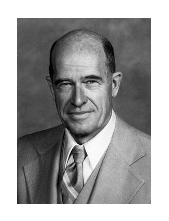
\includegraphics[width=0.9\linewidth]{WalterEvans.eps} 
    \caption*{\textbf{Walter Richard Evans}, (1920-1999),ingénieur, 
              automaticien américain. Il développa la méthode graphique, 
              qui porte son nom, permettant d'étudier les pôles des 
              systèmes asservis.}
\end{marginfigure}
%-------------------------------------------------------------------------------
pour l'étude des systèmes asservis.
%%%%%%%%%%%%%%%%%%%%%%%%%%%%%%%%%%%%%%%%%%%%%%%%%%%%%%%%%%%%%%%%%%%%%%%%%%%%%%%%
\paragraph{Exemple de carte de pôles et zéros d'une fonction de transfert}
%%%%%%%%%%%%%%%%%%%%%%%%%%%%%%%%%%%%%%%%%%%%%%%%%%%%%%%%%%%%%%%%%%%%%%%%%%%%%%%%
Soit $H(p)$ une fonction de transfert telle que,
%-------------------------------------------------------------------------------
\begin{align}
    H(p)=\dfrac{p-1}{p^2+2p+2}\label{eq-ft_carte}
\end{align}
%-------------------------------------------------------------------------------
Cette fonction de transfert possède un zéro réel ($z_1=1$) et deux 
pôles complexes conjugués ($p_{1,2}=-1\pm j$).
La forme factorisée de $H(p)$ est donc
%-------------------------------------------------------------------------------
\begin{align} 
    H(p)=\dfrac{p-1}{(p+1+j)(p+1-j)}
\end{align}
%-------------------------------------------------------------------------------
La~\cref{fig-carte} présente la carte des pôles de cette fonction de transfert.
%-------------------------------------------------------------------------------
\begin{figure}[!h]
    \center
    \tikzsetnextfilename{carte-chap_slci-ext}
    \input{tikz/carte-chap_slci.tex}
    \caption{Exemple d'une carte de pôles et zéros associés à la 
             fonction de transfert~\Cref{eq-ft_carte}\label{fig-carte}}
\end{figure}
%-------------------------------------------------------------------------------
%%%%%%%%%%%%%%%%%%%%%%%%%%%%%%%%%%%%%%%%%%%%%%%%%%%%%%%%%%%%%%%%%%%%%%%%%%%%%%%%
%%%%%%%%%%%%%%%%%%%%%%%%%%%%%%%%%%%%%%%%%%%%%%%%%%%%%%%%%%%%%%%%%%%%%%%%%%%%%%%%
%\subsection{Notion de pôles dominants}
%%%%%%%%%%%%%%%%%%%%%%%%%%%%%%%%%%%%%%%%%%%%%%%%%%%%%%%%%%%%%%%%%%%%%%%%%%%%%%%%
%%%%%%%%%%%%%%%%%%%%%%%%%%%%%%%%%%%%%%%%%%%%%%%%%%%%%%%%%%%%%%%%%%%%%%%%%%%%%%%%
%Soient $p_1,\ldots,p_n$ les pôles d'un système stable\footnote{À partir 
%des résultats obtenus dans ce chapitre il est déjà clair que la stabilité
%d'un système dépend également des pôles de sa fonction de transfert}.
%Le pôle $p_i$ est dit dominant si la valeur absolue
%de sa partie réelle est largement plus petite que celle de tout autre pôles 
%du système\footnote{Dans la pratique un rapport de 5 est 
%suffisant pour considérer une domination d'un pôle sur les autres}
%-------------------------------------------------------------------------------
%\begin{bequation}[ams align]
%	\big|\Re{p_i}\big| \ll \big|\Re{p_j}\big|\;\; \forall j\neq i
%\end{bequation}
%-------------------------------------------------------------------------------
%Pour observer l'influence d'un pôle dominant sur 
%la réponse temporelle d'un système linéaire, nous
%nous allons l'illustrer par l'étude d'une fonction 
%de transfert du second ordre en régime apériodique.
%Une telle fonction de transfert est équivalente à deux
%systèmes du premier ordre en série.

%Prenons l'exemple de la fonction de transfert définie par  
%\[
%       H(p)=\dfrac{5}{(p+1)(5p+1)}
%\]
%et de décomposition en éléments simples telle que :
%\[
%       H(p)=\dfrac{A}{p+1}+\dfrac{B}{5p+1}
%\]
%Par identification on peut écrire $H(p)$ en fonction de
%deux fonctions de transferts $H_1(p)$ et $H_2(p)$ tel que :
%-------------------------------------------------------------------------------
%\begin{align*}
%	H(p)&=H_1(p)-H_2(p)\\
%	H_1(p)&=\dfrac{6.25}{5p+1}\\
%	H_2(p)&=\dfrac{1.25}{p+1}
%\end{align*}
%-------------------------------------------------------------------------------
%Par définition, le pôle dominant est donné par $H_1(p)$.
%Pour observer son effet traçons les réponses indicielles 
%de ces trois fonctions de transfert.
%-------------------------------------------------------------------------------
%\begin{figure}[!h]
%    \centering
%    \tikzsetnextfilename{pole_dominant-chap_slci-ext}
%    \input{tikz/pole_dominant-chap_slci.tex}
%    \caption{}
%\end{figure}
%-------------------------------------------------------------------------------
%-------------------------------------------------------------------------------
%Exercice
%La même approche appliquée pour la fonction cosinus, nous donne :
%-------------------------------------------------------------------------------
%\begin{bequation}[ams align]
%    \laplace{\cos{\omega t}\cdot u(t)}=\dfrac{p}{p^2+\omega^2}
%\end{bequation}
%-------------------------------------------------------------------------------
%Exercice
%%%%%%%%%%%%%%%%%%%%%%%%%%%%%%%%%%%%%%%%%%%%%%%%%%%%%%%%%%%%%%%%%%%%%%%%%%%%%%%%
%\paragraph{Transformée d'une sinuso\"ide amortie}
%%%%%%%%%%%%%%%%%%%%%%%%%%%%%%%%%%%%%%%%%%%%%%%%%%%%%%%%%%%%%%%%%%%%%%%%%%%%%%%%
%La transformée de Laplace d'un signal sinuso\"idal amortie s'écrit :
%-------------------------------------------------------------------------------
%\begin{align*}
%\laplace{e^{-at}\sin{\omega t}\cdot u(t)}&=\int_{0}^{+\infty}e^{-pt}e^{-at}
%\dfrac{e^{\jw t}-e^{-\jw t}}{2j}\dd{t}\\
%&=\dfrac{1}{2j}\int_{0}^{+\infty}e^{-((p+a)-\jw)t}\dd{t} - 
%\dfrac{1}{2j}\int_{0}^{+\infty}e^{-((p+a)+\jw)t}\dd{t} \\
%&=\dfrac{1}{2j}\left( \dfrac{1}{(p+a)-\jw}-\dfrac{1}{(p+a)+\jw}\right)\\
%&=\dfrac{\omega}{(p+a)^2+\omega^2}
%\end{align*}
%-------------------------------------------------------------------------------
%ou encore
%-------------------------------------------------------------------------------
%\begin{bequation}[ams align]
%    \laplace{e^{-at}\sin{\omega t}\cdot u(t)}=\dfrac{\omega}{(p+a)^2+\omega^2}
%\end{bequation}
%-------------------------------------------------------------------------------
%Remarquons que pour cette transformée, nous aurions pu faire usage
%de la propriété du théorème de l'amortissement (c.f propriétés du paragraphe 
%précédent).
\newpage
%%%%%%%%%%%%%%%%%%%%%%%%%%%%%%%%%%%%%%%%%%%%%%%%%%%%%%%%%%%%%%%%%%%%%%%%%%%%%%%%
%%%%%%%%%%%%%%%%%%%%%%%%%%%%%%%%%%%%%%%%%%%%%%%%%%%%%%%%%%%%%%%%%%%%%%%%%%%%%%%%
%%%%%%%%%%%%%%%%%%%%%%%%%%%%%%%%%%%%%%%%%%%%%%%%%%%%%%%%%%%%%%%%%%%%%%%%%%%%%%%%
\section{Exercices du chapitre}
%%%%%%%%%%%%%%%%%%%%%%%%%%%%%%%%%%%%%%%%%%%%%%%%%%%%%%%%%%%%%%%%%%%%%%%%%%%%%%%%
%%%%%%%%%%%%%%%%%%%%%%%%%%%%%%%%%%%%%%%%%%%%%%%%%%%%%%%%%%%%%%%%%%%%%%%%%%%%%%%%
%%%%%%%%%%%%%%%%%%%%%%%%%%%%%%%%%%%%%%%%%%%%%%%%%%%%%%%%%%%%%%%%%%%%%%%%%%%%%%%%
\small
%{\tikzset{external/export=false} 
\makeatletter
\newcount\my@repeat@count
\newcommand{\myrepeat}[2]{%
    \begingroup
    \my@repeat@count=\z@
    \@whilenum\my@repeat@count<#1\do{#2\advance\my@repeat@count\@ne}%
    \endgroup
}
\makeatother
\newcommand{\mystar}{{\color{col1}\fontfamily{lmr}\selectfont$\star$}}
\newcommand{\facile}{\marginpar{\myrepeat{1}{\mystar}}}
\newcommand{\moyen}{\marginpar{\myrepeat{2}{\mystar}}}
\newcommand{\difficile}{\marginpar{\myrepeat{3}{\mystar}}}
\newcommand{\tresdifficile}{\marginpar{\myrepeat{4}{\mystar}}}
%%%%%%%%%%%%%%%%%%%%%%%%%%%%%%%%%%%%%%%%%%%%%%%%%%%%%%%%%%%%%%%%%%%%%%%%%%%%%%%%
%%%%%%%%%%%%%%%%%%%%%%%%%%%%%%%%%%%%%%%%%%%%%%%%%%%%%%%%%%%%%%%%%%%%%%%%%%%%%%%%
\moyen\exercice{L'impulsion de Dirac approchée}
%%%%%%%%%%%%%%%%%%%%%%%%%%%%%%%%%%%%%%%%%%%%%%%%%%%%%%%%%%%%%%%%%%%%%%%%%%%%%%%%
%%%%%%%%%%%%%%%%%%%%%%%%%%%%%%%%%%%%%%%%%%%%%%%%%%%%%%%%%%%%%%%%%%%%%%%%%%%%%%%%
L'impulsion de Dirac peut être approchée par la fonction porte 
$\delta_a(t)$ définie par le graphe ci-contre.

%%%%%%%%%%%%%%%%%%%%%%%%%%%%%%%%%%%%%%%%%%%%%%%%%%%%%%%%%%%%%%%%%%%%%%%%%%%%%%%%
\question{Décomposer $\delta_a(t)$ à l'aide de fonctions échelons.}
%%%%%%%%%%%%%%%%%%%%%%%%%%%%%%%%%%%%%%%%%%%%%%%%%%%%%%%%%%%%%%%%%%%%%%%%%%%%%%%%
%-------------------------------------------------------------------------------
\begin{marginfigure}
    \centering
    \tikzsetnextfilename{fonction_porte-chap-slci-ext}
    \begin{tikzpicture}[baseline=0]
   \begin{axis}[
        height=4cm,
        width=5cm,
        axis x line=center,
        axis y line=center,
        xmin=-1,
        xmax=5,
        ymin=-0.5,
        ymax=2.0,
        xlabel={$t$},
        ylabel={$\delta_a(t)$},
        xlabel style={below right},
        ylabel style={left},
        yticklabels={$\dfrac{1}{a}$},
        ytick={1},
        y tick label style={anchor=east},
        xticklabels={$a$},
        xtick={2},
        x tick label style={anchor=north},
        ]
        \addplot [very thick,col1,const plot] coordinates 
        {(-1,0.01) (0,0.01) (0,1) (2,1)  (2,0.01) (5,0.01) };
        \end{axis}
\end{tikzpicture}

\end{marginfigure}
%-------------------------------------------------------------------------------

%%%%%%%%%%%%%%%%%%%%%%%%%%%%%%%%%%%%%%%%%%%%%%%%%%%%%%%%%%%%%%%%%%%%%%%%%%%%%%%%
\question{Donner sa transformée de Laplace en fonction du paramètre $a$.}
%%%%%%%%%%%%%%%%%%%%%%%%%%%%%%%%%%%%%%%%%%%%%%%%%%%%%%%%%%%%%%%%%%%%%%%%%%%%%%%%

%%%%%%%%%%%%%%%%%%%%%%%%%%%%%%%%%%%%%%%%%%%%%%%%%%%%%%%%%%%%%%%%%%%%%%%%%%%%%%%%
\question{En considérant la limite $a\rightarrow0$, montrer que la transformée
          de Laplace de $\delta_a(t)$ tend bien vers 1.}
%%%%%%%%%%%%%%%%%%%%%%%%%%%%%%%%%%%%%%%%%%%%%%%%%%%%%%%%%%%%%%%%%%%%%%%%%%%%%%%%

%%%%%%%%%%%%%%%%%%%%%%%%%%%%%%%%%%%%%%%%%%%%%%%%%%%%%%%%%%%%%%%%%%%%%%%%%%%%%%%%
\question{Soit la fonction $g_a(t)$ définie par le graphe ci-contre. 
          Décomposer $g_a(t)$ à l'aide de fonctions échelons et/ou rampes. Donner sa 
          transformée de Laplace.}
%%%%%%%%%%%%%%%%%%%%%%%%%%%%%%%%%%%%%%%%%%%%%%%%%%%%%%%%%%%%%%%%%%%%%%%%%%%%%%%%
%-------------------------------------------------------------------------------
\begin{marginfigure}
    \centering
    \tikzsetnextfilename{fonction_creneau-chap-slci-ext}
    \input{tikz/fonction_creneau-chap-slci.tex}
\end{marginfigure}
%-------------------------------------------------------------------------------

%}
\setcounter{numexos}{0}
\normalsize
\newpage
\restoregeometry
\captionsetup{width=0.9\linewidth,labelfont=bf}
%%%%%%%%%%%%%%%%%%%%%%%%%%%%%%%%%%%%%%%%%%%%%%%%%%%%%%%%%%%%%%%%%%%%%%%%%%%%%%%%
%%%%%%%%%%%%%%%%%%%%%%%%%%%%%%%%%%%%%%%%%%%%%%%%%%%%%%%%%%%%%%%%%%%%%%%%%%%%%%%%
%%%%%%%%%%%%%%%%%%%%%%%%%%%%%%%%%%%%%%%%%%%%%%%%%%%%%%%%%%%%%%%%%%%%%%%%%%%%%%%%
\section{Corrigé des exercices}
%%%%%%%%%%%%%%%%%%%%%%%%%%%%%%%%%%%%%%%%%%%%%%%%%%%%%%%%%%%%%%%%%%%%%%%%%%%%%%%%
%%%%%%%%%%%%%%%%%%%%%%%%%%%%%%%%%%%%%%%%%%%%%%%%%%%%%%%%%%%%%%%%%%%%%%%%%%%%%%%%
%%%%%%%%%%%%%%%%%%%%%%%%%%%%%%%%%%%%%%%%%%%%%%%%%%%%%%%%%%%%%%%%%%%%%%%%%%%%%%%%
\small
%%%%%%%%%%%%%%%%%%%%%%%%%%%%%%%%%%%%%%%%%%%%%%%%%%%%%%%%%%%%%%%%%%%%%%%%%%%%%%%%
%%%%%%%%%%%%%%%%%%%%%%%%%%%%%%%%%%%%%%%%%%%%%%%%%%%%%%%%%%%%%%%%%%%%%%%%%%%%%%%%
\exercice{L'impulsion de Dirac approchée}
%%%%%%%%%%%%%%%%%%%%%%%%%%%%%%%%%%%%%%%%%%%%%%%%%%%%%%%%%%%%%%%%%%%%%%%%%%%%%%%%
%%%%%%%%%%%%%%%%%%%%%%%%%%%%%%%%%%%%%%%%%%%%%%%%%%%%%%%%%%%%%%%%%%%%%%%%%%%%%%%%
%%%%%%%%%%%%%%%%%%%%%%%%%%%%%%%%%%%%%%%%%%%%%%%%%%%%%%%%%%%%%%%%%%%%%%%%%%%%%%%%
\question{}
%%%%%%%%%%%%%%%%%%%%%%%%%%%%%%%%%%%%%%%%%%%%%%%%%%%%%%%%%%%%%%%%%%%%%%%%%%%%%%%%
%-------------------------------------------------------------------------------
\begin{figure}[!h]
    \centering
    \tikzsetnextfilename{fonction_porte_decomposition-chap-slci-ext}
    \input{tikz/fonction_porte_decomposition-chap-slci.tex}
\end{figure}
%-------------------------------------------------------------------------------
La fonction $\delta_a(t)$ est simplement donnée par 
\[
    \color{col1}p_a(t)
    =\color{col4}\dfrac{1}{a}u(t)\color{col3}-\dfrac{1}{a}u(t-a)
    =\normalcolor\dfrac{1}{a}\left(u(t)-u(t-a)\right)
\] 
où $u(t)$ est la fonction échelon unité.

%%%%%%%%%%%%%%%%%%%%%%%%%%%%%%%%%%%%%%%%%%%%%%%%%%%%%%%%%%%%%%%%%%%%%%%%%%%%%%%%
\question{}
%%%%%%%%%%%%%%%%%%%%%%%%%%%%%%%%%%%%%%%%%%%%%%%%%%%%%%%%%%%%%%%%%%%%%%%%%%%%%%%%
On rappel la transformée de Laplace d'une fonction retardée :
\[
    \laplace{f(t-\tau)} = e^{-\tau p}F(p)
\]
La transformée de Laplace de $\delta_a(t)$ est donc donnée par : 
\[
    \Delta_a(p) = \laplace{\delta_a(t)}
                = \dfrac{1}{a}\left(\laplace{u(t)}-\laplace{u(t-a)}\right)
                = \dfrac{1}{ap}(1-e^{-ap})
\]
%%%%%%%%%%%%%%%%%%%%%%%%%%%%%%%%%%%%%%%%%%%%%%%%%%%%%%%%%%%%%%%%%%%%%%%%%%%%%%%%
\question{}
%%%%%%%%%%%%%%%%%%%%%%%%%%%%%%%%%%%%%%%%%%%%%%%%%%%%%%%%%%%%%%%%%%%%%%%%%%%%%%%%
Le développement limité d'ordre 1 de $e^{x}=1+x+o\left(x\right)$ permet de
déterminer la limite pour $a\rightarrow0$ de la transformée de Laplace de 
$\delta_a(t)$. En effet, 
\[
    \lim_{a\to0} \Delta_a(p) = \dfrac{1}{ap}(1-1+ap)=1.
\]
Puisque la transformée de Laplace d'une impulsion de Dirac est égale à 1, on a
bien vérifié que $\lim_{a\to0} \delta_a(p)=\delta(t)$ où $\delta(t)$ est 
l'impulsion de Dirac.

%%%%%%%%%%%%%%%%%%%%%%%%%%%%%%%%%%%%%%%%%%%%%%%%%%%%%%%%%%%%%%%%%%%%%%%%%%%%%%%%
\question{Soit la fonction $g_a(t)$ définie par le graphe ci-contre. 
          Décomposer $g_a(t)$ à l'aide de fonctions échelons et/ou rampes. Donner sa 
          transformée de Laplace.}
%%%%%%%%%%%%%%%%%%%%%%%%%%%%%%%%%%%%%%%%%%%%%%%%%%%%%%%%%%%%%%%%%%%%%%%%%%%%%%%%
%-------------------------------------------------------------------------------
\begin{marginfigure}
    \centering
    \tikzsetnextfilename{fonction_creneau-chap-slci-ext}
    \begin{tikzpicture}[baseline=0]
   \begin{axis}[
   height=4cm,
   width=5cm,
      axis x line=center,
        axis y line=center,
        xmin=-1,
        xmax=5,
        ymin=-1.5,
        ymax=2.0,
        xlabel={$t$},
        ylabel={$g_a(t)$},
        xlabel style={below right},
        ylabel style={left},
        yticklabels={$\dfrac{1}{a}$},
        ytick={1},
        y tick label style={left},
        xticklabels={$\tau+a$,$\tau+2a$},
        xtick={2,4},
        x tick label style={below},
        ]
        \addplot [very thick,col1,domain=-1:0, samples=50]{0.01};
        \addplot [very thick,col1,domain=0:2, samples=50]{0.5*x};
        \addplot [very thick,col1,domain=2:4, samples=50]{-0.5*x+2};
        \addplot [very thick,col1,domain=4:5, samples=50]{0.01};
        \end{axis}
\end{tikzpicture}

\end{marginfigure}
%-------------------------------------------------------------------------------

\[
    g_a(t)=\dfrac{1}{a(\tau+a)}r(t)-\dfrac{2}{a(\tau+a)}r(t-(\tau+a))+\dfrac{1}{a(\tau+a)}r(t-(\tau+2a))
\]

\[
    g_a(t)=\dfrac{t}{a(\tau+a)}u(t)
\]

\[
    -\dfrac{t}{a(\tau+a)}-\dfrac{1}{\tau+a}-\dfrac{1}{a}=\dfrac{t}{a(\tau+a)}+f_2(t)
\]

\[
    -\dfrac{2t-(\tau+2a)}{a(\tau+a)}=f_2(t)
\]

\[
    g_a(t)=\dfrac{t}{a(\tau+a)}u(t)-\dfrac{2t-(\tau+2a)}{a(\tau+a)}u(t-(\tau+a))
\]

\[
    f_3(t)=\dfrac{t-(\tau+2a)}{a(\tau+a)}
\]

\[
    g_a(t)=\dfrac{t}{a(\tau+a)}u(t)-\dfrac{2t-(\tau+2a)}{a(\tau+a)}u(t-(\tau+a))+\dfrac{t-(\tau+2a)}{a(\tau+a)}u(t-(\tau+2a))
\]

\[
    g_a(t)=\dfrac{1}{a(\tau+a)}\left(t-(2t-(\tau+2a))u(t-(\tau+a))+(t-(\tau+2a))u(t-(\tau+2a))\right)
\]

\footnotesize
\[
    \laplace{g_a(t)}=\dfrac{1}{a(\tau+a)}\left(   \dfrac{1}{p^2}-\dfrac{2e^{-(\tau+a)p}}{p^2}+\dfrac{(\tau+2a)e^{-(\tau+a)p}}{p}
                                                + \dfrac{e^{-(\tau+2a)p}}{p^2} - \dfrac{(\tau+2a)e^{-(\tau+2a)p}}{p} \right)
\]
\[
     \laplace{g_a(t)}=\dfrac{1}{a(\tau+a)}\left( \dfrac{1}{p^2}\left(1-2e^{-(\tau+a)p}+e^{-(\tau+2a)p}\right) 
                                           + \dfrac{(\tau+2a)}{p}\left(e^{-(\tau+a)p}-e^{-(\tau+2a)p} \right) \right)
\]


\[
    e^{-(\tau+a)p}=e^{-\tau p}e^{-ap}=e^{-\tau p}\left(1-ap+\dfrac{(ap)^2}{2}\right)
\]

\[
    e^{-(\tau+2a)p}=e^{-\tau p}e^{-2ap}=e^{-\tau p}\left(1-2ap+2(ap)^2\right)
\]

\[
    1-2e^{-(\tau+a)p}+e^{-(\tau+2a)p}=1-e^{-\tau p}\left(1-ap+\dfrac{(ap)^2}{2}\right)+e^{-\tau p}\left(1-2ap+2(ap)^2\right)
\]

\[
    1-2e^{-(\tau+a)p}+e^{-(\tau+2a)p}=1-ape^{-\tau p}+\dfrac{3}{2}(ap)^2e^{-\tau p}
\]

\[
    e^{-(\tau+a)p}=e^{-\tau p}e^{-ap}=e^{-\tau p}\left(1-ap\right)
\]

\[
    e^{-(\tau+2a)p}=e^{-\tau p}e^{-ap}=e^{-\tau p}\left(1-2ap\right)
\]

\[
    e^{-(\tau+a)p}-e^{-(\tau+2a)p}=ape^{-\tau p}
\]

\[
    \laplace{g_a(t)}=\dfrac{1}{a(\tau+a)}\left(\right)
\]


\[
    g_a(t)=\dfrac{t}{a(\tau+a)}\left(u(t)-u(t-(\tau+a))\right) - \left(\dfrac{t-(\tau+2a)}{a(\tau+a)}\right)\left(u(t-(\tau+a))-u(t-(\tau+2a))\right)
\]

\[
    \laplace{g_a(t)}=\dfrac{1}{a(\tau+a)p^2}\left(1-e^{-(\tau+a)p}\right) - \dfrac{1}{a(\tau+a)}\left(\dfrac{1}{p^2}-\dfrac{(\tau+2a)}{p}\right)\left(e^{-(\tau+a)p}-e^{-(\tau+2a)p}\right)
\]

\normalsize
\restoregeometry
\captionsetup{width=0.9\linewidth,labelfont=bf}
%%%%%%%%%%%%%%%%%%%%%%%%%%%%%%%%%%%%%%%%%%%%%%%%%%%%%%%%%%%%%%%%%%%%%%%%%%%%%%%%
%%%%%%%%%%%%%%%%%%%%%%%%%%%%%%%%%%%%%%%%%%%%%%%%%%%%%%%%%%%%%%%%%%%%%%%%%%%%%%%%
%%%%%%%%%%%%%%%%%%%%%%%%%%%%%%%%%%%%%%%%%%%%%%%%%%%%%%%%%%%%%%%%%%%%%%%%%%%%%%%%
%%%%%%%%%%%%%%%%%%%%%%%%%%%%%%%%%%%%%%%%%%%%%%%%%%%%%%%%%%%%%%%%%%%%%%%%%%%%%%%%
%chap_slci.tex
                %1 SLCI                
%%%%%%%%%%%%%%%%%%%%%%%%%%%%%%%%%%%%%%%%%%%%%%%%%%%%%%%%%%%%%%%%%%%%%%%%%%%%%%%%%%%%%%%
%%%%%%%%%%%%%%%%%%%%%%%%%%%%%%%%%%%%%%%%%%%%%%%%%%%%%%%%%%%%%%%%%%%%%%%%%%%%%%%%%%%%%%%%%%%%%%%%%%%%%%%%
%%%%%%%%%%%%%%%%%%%%%%%%%%%%%%%%%%%%%%%%%%%%%%%%%%%%%%%%%%%%%%%%%%%%%%%%%%%%%%%%%%%%%%%%%%%%%%%%%%%%%%%%
\chapter[Schéma fonctionnels]{Schémas fonctionnels et graphes de fluence\label{chap-schemabloc}}
%%%%%%%%%%%%%%%%%%%%%%%%%%%%%%%%%%%%%%%%%%%%%%%%%%%%%%%%%%%%%%%%%%%%%%%%%%%%%%%%%%%%%%%
%%%%%%%%%%%%%%%%%%%%%%%%%%%%%%%%%%%%%%%%%%%%%%%%%%%%%%%%%%%%%%%%%%%%%%%%%%%%%%%%%%%%%%%%%%%%%%%%%%%%%%%%
%%%%%%%%%%%%%%%%%%%%%%%%%%%%%%%%%%%%%%%%%%%%%%%%%%%%%%%%%%%%%%%%%%%%%%%%%%%%%%%%%%%%%%%%%%%%%%%%%%%%%%%%

\minitoc
\newpage
%%%%%%%%%%%%%%%%%%%%%%%%%%%%%%%%%%%%%%%%%%%%%%%%%%%%%%%%%%%%%%%%%%%%%%%%%%%%%%%%%%%%%%%%%%%%%%%%%%%%%%%%
%%%%%%%%%%%%%%%%%%%%%%%%%%%%%%%%%%%%%%%%%%%%%%%%%%%%%%%%%%%%%%%%%%%%%%%%%%%%%%%%%%%%%%%
\section{Introduction}
%%%%%%%%%%%%%%%%%%%%%%%%%%%%%%%%%%%%%%%%%%%%%%%%%%%%%%%%%%%%%%%%%%%%%%%%%%%%%%%%%%%%%%%%%%%%%%%%%%%%%%%%
%%%%%%%%%%%%%%%%%%%%%%%%%%%%%%%%%%%%%%%%%%%%%%%%%%%%%%%%%%%%%%%%%%%%%%%%%%%%%%%%%%%%%%%
Dans ce chapitre, nous allons introduire un outil graphique pour faciliter 
la représentation des relations mathématiques entre les différents 
éléments constituants un \gls{slci}. Cet outil est le \textbf{schéma fonctionnel} ou 
également appelé \textbf{schéma-bloc}. Les schémas fonctionnels nous seront très 
utiles pour l'étude des systèmes asservis. Nous introduirons une algèbre de blocs permettant
de réduire les schémas-blocs de grande taille. Nous aborderons également le cas des entrées multiples. 

Dans une dernière partie nous introduirons 
les graphes de fluence, comme présenté dans~\cite{Ostertag}. Ces derniers 
sont moins utilisés pour l'étude des \gls{slci}, et peuvent donc être négligés 
dans une première lecture, l'algèbre qui lui est associée s'avère cependant bien plus 
éfficace et pourra être utilisée dans d'autres 
applications (ex : éléctronique, réseaux de neurones).


%%%%%%%%%%%%%%%%%%%%%%%%%%%%%%%%%%%%%%%%%%%%%%%%%%%%%%%%%%%%%%%%%%%%%%%%%%%%%%%%%%%%%%%%%%%%%%%%%%%%%%%%
%%%%%%%%%%%%%%%%%%%%%%%%%%%%%%%%%%%%%%%%%%%%%%%%%%%%%%%%%%%%%%%%%%%%%%%%%%%%%%%%%%%%%%%
\section{\'Eléments de base des schémas fonctionnels}
%%%%%%%%%%%%%%%%%%%%%%%%%%%%%%%%%%%%%%%%%%%%%%%%%%%%%%%%%%%%%%%%%%%%%%%%%%%%%%%%%%%%%%%%%%%%%%%%%%%%%%%%
%%%%%%%%%%%%%%%%%%%%%%%%%%%%%%%%%%%%%%%%%%%%%%%%%%%%%%%%%%%%%%%%%%%%%%%%%%%%%%%%%%%%%%%
Les schémas fonctionnels sont composés de quatre éléments de base:
\textbf{les flèches, les blocs, les comparateurs et sommateurs et les points de prélèvement}
%\begin{itemize}
%    \item les flèches.
%    \item les blocs.
%    \item les comparateurs et sommateurs.
%    \item les points de prélèvement.
%\end{itemize}

%\newpage
%%%%%%%%%%%%%%%%%%%%%%%%%%%%%%%%%%%
\paragraph{Flèche}
%%%%%%%%%%%%%%%%%%%%%%%%%%%%%%%%%%%
Les flèches donnent la direction de l'information (i.e du signal) au sein du schéma-blocs. 
Elles peuvent être ornées de la grandeur mathématique qui leurs sont associée. 
Celles-ci peuvent être des grandeurs temporelles ou dans le domaine de Laplace. 
\begin{center}
\tikzsetnextfilename{sb_fleche-chap1_ext}
\begin{tikzpicture}
    \draw[-latex] (-3,0) -- (-1,0) node[midway,above] {$e(t)$};
    \draw[-latex] (0,0) -- (2,0) node[midway,above] {$E(p)$};
\end{tikzpicture}    
\end{center}
Cependant, nous nous limiterons à l'usage de ces schémas fonctionnelles pour la représentation
de grandeur dans le domaine de Laplace.

Pour alléger la notation dans ce chapitre, nous omettrons 
très souvent la variable $p$ des grandeurs dans le domaine de Laplace désignées par une majuscule.

\newpage
%%%%%%%%%%%%%%%%%%%%%%%%%%%%%%%%%%%
\paragraph{Bloc}
%%%%%%%%%%%%%%%%%%%%%%%%%%%%%%%%%%%

Le bloc est la représentation d'une fonction de transfert entre deux grandeurs dans le domaine de Laplace.
Par exemple, la relation entre l'entrée $E$ et la sortie $S$ définit par la fonction de transfert $H$
qui s'écrit formellement, 
\begin{bequation}[ams align]
S = HE,\label{eq-ES}
\end{bequation}
est équivalente au schéma fonctionnel\footnote{Les schémas-blocs de ce document ont tous 
étaient réalisés avec les macros Ti\emph{k}Z (\verb?schemabloc?) écrit par R. Papanicola\cite{schemabloc}. 
\`A noter que des macros Ti\emph{k}Z (\verb?gfluence?) pour représenter les graphes de fluence 
de ce même chapitre, ont était fortement inspiré par ce même auteur.} 
suivant:

\begin{center}
\tikzsetnextfilename{sb_bloc-chap1_ext}
\begin{tikzpicture}
    \sbEntree{E1}
    \sbBloc[3]{B1}{$H$}{E1}
        \sbRelier[$E$]{E1}{B1}
    \sbSortie[3]{S1}{B1}
        \sbRelier[$S$]{B1}{S1}
\end{tikzpicture}    
\end{center}


%%%%%%%%%%%%%%%%%%%%%%%%%%%%%%%%%%%
\paragraph{Comparateur/Sommateur :}
%%%%%%%%%%%%%%%%%%%%%%%%%%%%%%%%%%%

Les comparateurs ou sommateurs permettent de représenter des opérations 
simples entre différentes grandeurs.
Nous parlerons respectivement de comparateur ou de sommateur dans le cas 
d'une différence ou d'une somme entre deux grandeurs. 


Par exemple, la relation 
$$
S = E_1-E_2 
$$
est équivalente au comparateur suivant :
\begin{center}
\tikzsetnextfilename{sb_comp-chap1_ext}
    \begin{tikzpicture}
        \coordinate (pt) at (0,-1);
        \sbEntree{E1}
        \sbComp[4.5]{comp}{E1}
        \sbRelier[$E_1$]{E1}{comp}
        \sbSortie[2.5]{S}{comp}
        \sbRelier[$S$]{comp}{S}
        \draw[-latex] (comp|-0,-1.5) -- (comp.south) node[midway,left] {$E_2$};
    \end{tikzpicture}
\end{center}

De même la somme de deux grandeurs,
$$                                                                                                                            
S = E_1+E_2                                                                                                          
$$
est équivalente au sommateur suivant :
\begin{center}
\tikzsetnextfilename{sb_somm-chap1_ext}
    \begin{tikzpicture}
        \coordinate (pt) at (0,-1);
        \sbEntree{E1}
        \sbSumb[4.5]{comp}{E1}
        \sbRelier[$E_1$]{E1}{comp}
        \sbSortie[2.5]{S}{comp}
        \sbRelier[$S$]{comp}{S}
        \draw[-latex] (comp|-0,-1.5) -- (comp.south) node[midway,left] {$E_2$};
    \end{tikzpicture}
\end{center}

%%%%%%%%%%%%%%%%%%%%%%%%%%%%%%%%%%%
\paragraph{Point de prélèvement}
%%%%%%%%%%%%%%%%%%%%%%%%%%%%%%%%%%%

Un point de prélèvement (ou point de dérivation ou encore jonction) 
est un point d'une flèche où une information est prélevée ne modifiant pas sa valeur.
Par exemple, la jonction suivante (représentée par un point) donne lieu à deux branches auxquelles sont
associées la même grandeur $S$.

\begin{center}
\tikzsetnextfilename{sb_point-chap1_ext}
    \begin{tikzpicture} 
    \draw[fill=black] (1,0) circle[radius=2.0pt];
    \draw[-latex] (0, 0) -- (2, 0) node[above] {branche 1 : $S$};
    \draw         (1, 0) -- (1,-1);
    \draw[-latex] (1,-1) -- (0,-1) node[below] {branche 2 : $S$};
    \end{tikzpicture}
\end{center}

Dans cette configuration, la branche 1 est dite \og direct\fg et la branche 2 est dite de \og retour\fg.

%%%%%%%%%%%%%%%%%%%%%%%%%%%%%%%%%%%%%%%%%%%%%%%%%%%%%%%%%%%%%%%%%%%%%%%%%%%%%%%%%%%%%%%
%%%%%%%%%%%%%%%%%%%%%%%%%%%%%%%%%%%%%%%%%%%%%%%%%%%%%%%%%%%%%%%%%%%%%%%%%%%%%%%%%%%%%%%%%%%%%%%%%%%%%%%%
\section{Transformation des schémas fonctionnels}
%%%%%%%%%%%%%%%%%%%%%%%%%%%%%%%%%%%%%%%%%%%%%%%%%%%%%%%%%%%%%%%%%%%%%%%%%%%%%%%%%%%%%%%
%%%%%%%%%%%%%%%%%%%%%%%%%%%%%%%%%%%%%%%%%%%%%%%%%%%%%%%%%%%%%%%%%%%%%%%%%%%%%%%%%%%%%%%%%%%%%%%%%%%%%%%%

%%%%%%%%%%%%%%%%%%%%%%%%%%%%%%%%%%%%%%%%%%%%%%%%%%%%%%%%%%%%%%%%%%%%%%%%%%%%%%%%%%%%%%%
\subsection{Réduction de schéma-bloc}
%%%%%%%%%%%%%%%%%%%%%%%%%%%%%%%%%%%%%%%%%%%%%%%%%%%%%%%%%%%%%%%%%%%%%%%%%%%%%%%%%%%%%%%

%%%%%%%%%%%%%%%%%%%%%%%%%%%%%%%%%%%%%%%%%%
\paragraph{Blocs en série / produit}
%%%%%%%%%%%%%%%%%%%%%%%%%%%%%%%%%%%%%%%%%%
Lorsque les blocs sont placés en série, la fonction de transfert 
entre la sortie et l'entrée globale est le produit des fonctions de transfert mis en jeu.
Par exemple, les deux schémas fonctionnels suivants sont équivalents.

\begin{center}
\tikzsetnextfilename{sb_reduc_serie_1-chap1_ext}
    \begin{tikzpicture} 
    \sbEntree{E1}
    \sbBloc[3]{B1}{$H_1$}{E1}
        \sbRelier[$E$]{E1}{B1}
    \sbBloc[3]{B2}{$H_2$}{B1}
        \sbRelier{B1}{B2}
    \sbBloc[3]{B3}{$H_3$}{B2}
        \sbRelier{B2}{B3}
    \sbSortie[3]{S1}{B3}
        \sbRelier[$S$]{B3}{S1}
        \node at (B2|-0,-1) {\rotatebox{90}{\LARGE$\equiv$}};
    \end{tikzpicture}

\tikzsetnextfilename{sb_reduc_serie_2-chap1_ext}
    \begin{tikzpicture} 
    \sbEntree{E1}
        \sbBloc[3]{B1}{$H=H_1H_2H_3$}{E1}
        \sbRelier[$E$]{E1}{B1}
    \sbSortie[3]{S1}{B1}
        \sbRelier[$S$]{B1}{S1}
    \end{tikzpicture}
\end{center}

Nous laissons au lecteur la démonstration triviale à partir des relations mathématiques.


%%%%%%%%%%%%%%%%%%%%%%%%%%%%%%%%%%%%%%%%%%%%%%%%%%%%%%%%%%%%%%%%%%%%%%%%%%%%%%%%%%%%%%%
\paragraph{Blocs en parallèle} 
%%%%%%%%%%%%%%%%%%%%%%%%%%%%%%%%%%%%%%%%%%%%%%%%%%%%%%%%%%%%%%%%%%%%%%%%%%%%%%%%%%%%%%%

Lorsque les blocs sont placés en parallèle, la fonction de transfert 
entre la sortie et l'entrée globale est la somme des fonctions de transfert mis en jeu.
Par exemple, les deux schémas fonctionnels suivants sont équivalents.

\begin{center}
\tikzsetnextfilename{sb_reduc_para_1-chap1_ext}
    \begin{tikzpicture} 
    \sbEntree{E1}
    \sbBloc[6]{B1}{$H_1$}{E1}
    \sbRelier{E1}{B1}
    \sbDecaleNoeudy[-4]{B1}{r1}
    \sbBloc[-1.6]{B2}{$H_2$}{r1}
    \sbRelieryx{E1-B1}{B2.west}
    \sbDecaleNoeudy[4]{B1}{r2}
    \sbBloc[-1.6]{B3}{$H_3$}{r2}
    \sbRelieryx{E1-B1}{B3.west}
    \sbCompSum[5]{C1}{B1}{+}{+}{+}{ }
    \sbRelier{B1}{C1}
    \sbRelierxy{B2}{C1}
    \sbRelierxy{B3}{C1}
    \sbSortie[3]{S1}{C1}
    \sbRelier[$S$]{C1}{S1}
    \node at (E1|-2.0,0.35) {$E$};
    \node at (B3|-0,-2.75) {\rotatebox{90}{\LARGE$\equiv$}};
%    \draw[fill=black] (1.325,0) circle[radius=2.0pt];
    \end{tikzpicture}

\tikzsetnextfilename{sb_reduc_para_2-chap1_ext}
    \begin{tikzpicture} 
      \sbEntree{E1}
    \sbBloc[3]{B1}{$H=H_1+H_2+H_3$}{E1}
    \sbRelier[$E$]{E1}{B1}
    \sbSortie[3]{S1}{B1}
    \sbRelier[$S$]{B1}{S1}
    \end{tikzpicture}
\end{center}

La démonstration est également triviale.

%%%%%%%%%%%%%%%%%%%%%%%%%%%%%%%%%%%%%%%%%%%%%%%%%%%%%%%%%%%%%%%%%%%%%%%%%%%%%%%%%%%%%%%
\paragraph{La boucle de contre-réaction (positive ou négative)\label{sec-boucle}}
%%%%%%%%%%%%%%%%%%%%%%%%%%%%%%%%%%%%%%%%%%%%%%%%%%%%%%%%%%%%%%%%%%%%%%%%%%%%%%%%%%%%%%%

La boucle de contre-réaction\footnote{\og Positive or negative feedback\fg, chez nos 
collègues anglophones.} peut 
être réduite à une simple fonction de transfert.
Considérons un système définit par le schéma-bloc ci-dessous, composé 
des différents élements de bases.

\begin{center}
    \tikzsetnextfilename{boucle-chap1_ext}
    \begin{tikzpicture}
    \sbEntree{E}
    \sbCompSum[5.0]{comp}{E}{}{\pm}{+}{}
        \sbRelier[$E$]{E}{comp}
        \sbBloc[3.5]{B}{$H_1$}{comp}
        \sbRelier[$\epsilon$]{comp}{B}
        \sbSortie[5.0]{S}{B}
        \sbRelier[$S$]{B}{S}
    \sbDecaleNoeudy[4]{B}{r1}
    \sbBlocr[-1.6]{B2}{$H_2$}{r1}
    \sbRelieryx{B-S}{B2}
        \sbRelierxy[$M$]{B2}{comp}
\end{tikzpicture}
\end{center}
Notons l'utilisation du symbole $\pm$ pour envisager à la fois les 
comparateurs et sommateurs.

Déterminons la relation entre l'entrée $E$ et la sortie $S$ de ce système.
Pour celà réécrivons les relations linéaires simples issus de ce schéma-bloc.
On sait que :
\begin{align}
    \epsilon&=E\pm M \label{eq-fb.1}\\
    M&=H_2S       \label{eq-fb.2}\\
    S&=H_1\epsilon \label{eq-fb.3}
\end{align}
Introduisons l'\cref{eq-fb.2} dans~(\ref{eq-fb.1}) et le résulat ainsi obtenu dans~(\ref{eq-fb.3}):
\begin{align*}
    \epsilon&=E\pm H_2S \\
     S&=H_1\big(E\pm H_2S\big) \\
     S&=H_1E\pm H_1H_2S
\end{align*}
Regroupons les termes dépendant de la sortie ensemble pour déterminer 
la relation entre l'entrée et la sortie.

\begin{align*}
    S\big(1\mp H_1H_2\big)&=H_1E 
\end{align*}

On obtient alors la formule de Black\footnote{\index{Black, Harold}Harold Stephen Black (1898-1983) ingénieur, 
électronicien américain.}, 
reliant la sortie est l'entrée d'une boucle de contre-réaction :
\begin{bequation}[ams align]
    S&=\dfrac{H_1}{1\mp H_1H_2}E
\end{bequation}

Notons l'inversion du signe du dénominateur de la formule 
selon que la boucle est positive ou négative.

La boucle de contre-réaction est donc équivalente au schéma-bloc simplifié suivant :
\begin{center}
    \tikzsetnextfilename{boucle_eq-chap1_ext}
    \begin{tikzpicture}
        \sbEntree{E1}
        \sbBloc[3]{B1}{$\dfrac{H_1}{1\mp H_1H_2}$}{E1}
        \sbRelier[$E$]{E1}{B1}
        \sbSortie[3]{S1}{B1}
        \sbRelier[$S$]{B1}{S1}
    \end{tikzpicture}    
\end{center}


%%%%%%%%%%%%%%%%%%%%%%%%%%%%%%%%%%%%%%%%%%%%%%%%%%%%%%%%%%%%%%%%%%%%%%%%%%%%%%%%%%%%%%%%%%%%%%%%%%%%%%%%
\paragraph{Boucle de contre-réaction unitaire}
%%%%%%%%%%%%%%%%%%%%%%%%%%%%%%%%%%%%%%%%%%%%%%%%%%%%%%%%%%%%%%%%%%%%%%%%%%%%%%%%%%%%%%%%%%%%%%%%%%%%%%%%

Une boucle de contre-réaction unitaire est une boucle de contre-réaction sans 
fonction de transfert de retour (ex: dans le cas présenté précedemment $H_2=1$).

\begin{center}
    \tikzsetnextfilename{boucle_uni-chap1_ext}
    \begin{tikzpicture}
    \sbEntree{E}
    \sbComp[5.0]{comp}{E}
        \sbRelier[$E$]{E}{comp}
        \sbBloc[3.0]{B}{$H_1$}{comp}
        \sbRelier[$\epsilon$]{comp}{B}
        \sbSortie[5.0]{S}{B}
        \sbRelier[$S$]{B}{S}
    \sbRenvoi{B-S}{comp}{}
\end{tikzpicture}
\end{center}

La formule de Black se simplifie alors de la façon suivante :
\begin{bequation}[ams align]
    S&=\dfrac{H_1}{1+H_1}E
\end{bequation}

%%%%%%%%%%%%%%%%%%%%%%%%%%%%%%%%%%%%%%%%%%%%%%%%%%%%%%%%%%%%%%%%%%%%%%%%%%%%%%%%%%%%%%%%%%%%%%%%%%%%%%%%
%%%%%%%%%%%%%%%%%%%%%%%%%%%%%%%%%%%%%%%%%%%%%%%%%%%%%%%%%%%%%%%%%%%%%%%%%%%%%%%%%%%%%%%%%%%%%%%%%%%%%%%%
\subsection{Manipulation de schéma-bloc}
%%%%%%%%%%%%%%%%%%%%%%%%%%%%%%%%%%%%%%%%%%%%%%%%%%%%%%%%%%%%%%%%%%%%%%%%%%%%%%%%%%%%%%%%%%%%%%%%%%%%%%%%
%%%%%%%%%%%%%%%%%%%%%%%%%%%%%%%%%%%%%%%%%%%%%%%%%%%%%%%%%%%%%%%%%%%%%%%%%%%%%%%%%%%%%%%%%%%%%%%%%%%%%%%%
Nous allons ici présenter différentes manipulations que nous
pourront appliquer au schéma-bloc. Ces manipulations peuvent
être vues comme des opérations d'une \textbf{algèbre de blocs}.

%%%%%%%%%%%%%%%%%%%%%%%%%%%%%%%%%%%%%%%%%%%%%%%%%%%%%%%%%%ù
\paragraph{Déplacement d'un comparateur vers la gauche}
%%%%%%%%%%%%%%%%%%%%%%%%%%%%%%%%%%%%%%%%%%%%%%%%%%%%%%%%%%ù

Considérons le schéma-bloc suivant :
\begin{center}
    \tikzsetnextfilename{dep_comp1-chap1_ext}
    \begin{tikzpicture}
        \coordinate (pt) at (0,-1);
        \sbEntree{E1}
        \sbBloc[4.0]{K}{$K$}{E1}
        \sbRelier[$E$]{E1}{K}
        \sbComp[6]{comp}{K}
        \sbRelier[$X_1$]{K}{comp}
        \sbBloc[3.0]{G}{$G$}{comp}
        \sbRelier[$\epsilon$]{comp}{G}
        \sbSortie[2.5]{S}{G}
        \sbRelier[$S$]{G}{S}
        \draw[-latex] (comp|-0,-1.5) -- (comp.south) node[midway,left] {$X_2$};
    \end{tikzpicture}
\end{center}

Pour pouvoir déplacer le comparateur vers la gauche, 
il faut introduire le bloc $K$ dans la chaine direct.
En conséquence, la chaîne de retour doit être modifiée pour ne pas affecter la sortie globale $S$.
Le schéma fonctionnel précédent est donc équivalent au schéma ci-dessous :

\begin{center}
    \tikzsetnextfilename{dep_comp2-chap1_ext}
    \begin{tikzpicture}
        \sbEntree{E1}
        \sbComp[4]{comp}{E1}
        \sbRelier[$E$]{E1}{comp}
        \sbBloc[3.0]{G}{$KG$}{comp}
        \sbRelier[$\epsilon$]{comp}{G}
        \sbSortie[2.5]{S}{G}
        \sbRelier[$S$]{G}{S}
        \sbDecaleNoeudy[4]{G}{r1}
        \sbBlocr[-1.5]{B2}{$\dfrac{1}{K}$}{r1}
        \sbRelierxy[$X_2$]{B2}{comp}
    \end{tikzpicture}
\end{center}


Dans le cas particulier où les deux branches du comparateur sont toutes les deux affectées par la même 
fonction de transfert, il suffit de déplacer la fonction de transfert après le comparateur. 
Par exemple, les deux schémas-blocs suivants sont équivalents: 

\begin{center}
    \tikzsetnextfilename{dep_comp3-chap1_ext}
    \begin{tikzpicture}
        \begin{scope}[local bounding box=scope1]
            \sbEntree{E1}
            \sbBloc[4.0]{K}{$K$}{E1}
            \sbRelier[$E$]{E1}{K}
            \sbComp[6]{comp}{K}
            \sbRelier[$X_1$]{K}{comp}
            \sbBloc[3.0]{G}{$G$}{comp}
            \sbRelier[$\epsilon$]{comp}{G}
            \sbSortie[2.5]{S}{G}
            \sbRelier[$S$]{G}{S}
            \sbDecaleNoeudy[4]{G}{r1}
            \sbBlocr[-1.5]{B2}{$K$}{r1}
            \sbRelierxy[$X_2$]{B2}{comp}
            \node at ( $(S)+(1,-0.75)$) {\LARGE$\equiv$};
        \end{scope}
%    \end{tikzpicture}
%    \tikzsetnextfilename{dep_comp4-chap1_ext}
%    \begin{tikzpicture}
        \begin{scope}[shift={($(scope1.east)+(-3,0.8)$)}]
            \sbEntree[8.0]{E1}
            \sbComp[4.0]{comp}{E1}
            \sbRelier[$E$]{E1}{comp}
            \sbBloc[3.0]{G}{$KG$}{comp}
            \sbRelier[$\epsilon$]{comp}{G}
            \sbSortie[2.5]{S}{G}
            \sbRelier[$S$]{G}{S}
            \draw[-latex] (comp|-0,-1.5) -- (comp.south) node[midway,left] {$X_2$};
        \end{scope}
    \end{tikzpicture}
\end{center}

%%%%%%%%%%%%%%%%%%%%%%%%%%%%%%%%%%%%%%%%%%%%%%%%%%%%%%%%%%ù
\paragraph{Déplacement d'un point de prélèvement vers la droite}
%%%%%%%%%%%%%%%%%%%%%%%%%%%%%%%%%%%%%%%%%%%%%%%%%%%%%%%%%%ù

Considérons le schéma-bloc suivant :
\begin{center}
    \tikzsetnextfilename{dep_jonc1-chap1_ext}
    \begin{tikzpicture}
        \sbEntree[7.0]{E1}
        \sbBloc[4.0]{K1}{$K$}{E1}
        \sbRelier[$E$]{E1}{K1}
        \sbBloc[2.0]{H1}{$H_1$}{K1}
        \sbRelier{K1}{H1}
        \sbDecaleNoeudy[4]{K1}{r1}
        \sbBloc[-1.5]{K2}{$K$}{r1}
        \sbRelieryx{E1-K1}{K2.west}
        \sbBloc[2.0]{H2}{$H_2$}{K2}
        \sbRelier{K2}{H2}
        \sbSortie[3.0]{S1}{H1}
        \sbRelier[$S_1$]{H1}{S1}
        \sbSortie[3.0]{S2}{H2}
        \sbRelier[$S_2$]{H2}{S2}
    \end{tikzpicture}
\end{center}                                                                                                                  
Il est aisé de déplacer le bloc $K$ devant le point de prélèvement:  
\begin{center}
    \tikzsetnextfilename{dep_jonc2-chap1_ext}
    \begin{tikzpicture}
        \sbEntree[1.0]{E1}
        \sbBloc[4.0]{K}{$K$}{E1}
        \sbRelier[$E$]{E1}{K}
        \sbBloc[3.0]{G}{$H_1$}{K}
        \sbRelier{K}{G}
        \sbDecaleNoeudy[4]{G}{r1}
        \sbBloc[-1.5]{G2}{$H_2$}{r1}
        \sbRelieryx{K-G}{G2.west}
        \sbSortie[3.0]{S1}{G}
        \sbRelier[$S_1$]{G}{S1}
        \sbSortie[3.0]{S2}{G2}
        \sbRelier[$S_2$]{G2}{S2}
    \end{tikzpicture}
\end{center}

Dans le cas particulier où seul une branche est affectée par le bloc, il faut réduire la branche non affectée après avoir 
déplacer le point de prélèvement. Ansi les deux schémas-blocs ci-dessous sont équivalents:

\begin{center}
    \tikzsetnextfilename{dep_jonc3-chap1_ext}
    \begin{tikzpicture}
        \begin{scope}[local bounding box=scope1]
            \sbEntree[1.0]{E1}
            \sbBloc[4.0]{K}{$K$}{E1}
            \sbRelier[$E$]{E1}{K}
            \sbBloc[3.0]{G}{$H_1$}{K}
            \sbRelier{K}{G}
            \sbDecaleNoeudy[4]{G}{r1}
            \sbBloc[-1.5]{G2}{$H_2$}{r1}
            \sbRelieryx{E1-K}{G2.west}
            \sbSortie[3.0]{S1}{G}
            \sbRelier[$S_1$]{G}{S1}
            \sbSortie[3.0]{S2}{G2}
            \sbRelier[$S_2$]{G2}{S2}
            \node at ( $(S1)+(1,-0.75)$) {\LARGE$\equiv$};
        \end{scope}
%    \end{tikzpicture}
%    \tikzsetnextfilename{dep_jonc4-chap1_ext}
%    \begin{tikzpicture}
        \begin{scope}[shift={($(scope1.east)+(-0.25,0.8)$)}]
            \sbEntree[1.0]{E1}
            \sbBloc[4.0]{K}{$K$}{E1}
            \sbRelier[$E$]{E1}{K}
            \sbBloc[3.0]{G}{$H_1$}{K}
            \sbRelier{K}{G}
            \sbDecaleNoeudy[4]{G}{r1}
            \sbBloc[-1.5]{G2}{$\dfrac{H_2}{K}$}{r1}
            \sbRelieryx{K-G}{G2.west}
            \sbSortie[3.0]{S1}{G}
            \sbRelier[$S_1$]{G}{S1}
            \sbSortie[3.0]{S2}{G2}
            \sbRelier[$S_2$]{G2}{S2}
        \end{scope}
    \end{tikzpicture}
\end{center}

%%%%%%%%%%%%%%%%%%%%%%%%%%%%%%%%%%%%%%%%%%%%%%%%%%%%%%%%%%%%%%%%%%%%%%%%%%%%%%%%%%%%%%%%%%%%%%%%%%%%%%%%
%%%%%%%%%%%%%%%%%%%%%%%%%%%%%%%%%%%%%%%%%%%%%%%%%%%%%%%%%%%%%%%%%%%%%%%%%%%%%%%%%%%%%%%%%%%%%%%%%%%%%%%%
\section{Cas d'entrées multiples}
%%%%%%%%%%%%%%%%%%%%%%%%%%%%%%%%%%%%%%%%%%%%%%%%%%%%%%%%%%%%%%%%%%%%%%%%%%%%%%%%%%%%%%%%%%%%%%%%%%%%%%%%
%%%%%%%%%%%%%%%%%%%%%%%%%%%%%%%%%%%%%%%%%%%%%%%%%%%%%%%%%%%%%%%%%%%%%%%%%%%%%%%%%%%%%%%%%%%%%%%%%%%%%%%%

Dans le cas d'un système possédant plusieurs entrées, il est possible de simplifier 
le problème en appliqant le principe de superposition. La réponse totale devient alors la somme
des réponses individuelles de chaque entrée lorsque toutes les autres sont considérées comme nulles.

Considérons le schéma-blocs suivant :
\begin{center}                                                                                                                
    \tikzsetnextfilename{reduc_mult1-chap1_ext}
\begin{tikzpicture}                                                                                                           
    \sbEntree{E}
    \sbComp{a}{E}
    \sbRelier[$E$]{E}{a}
    \sbBloc{b}{$H_1$}{a}
    \sbRelier{a}{b}
    \sbCompSum{d}{b}{+}{}{+}{}
    \sbRelier{b}{d}
    \sbBlocL{e}{$H_2$}{d}
    \sbSortie[5]{S1}{e}
    \sbRelier{e}{S1}
    \sbNomLien[0.8]{S1}{$S$}
    \sbDecaleNoeudy{e}{v}
    \sbBlocr{r2}{$R_1$}{v}
    \sbRelieryx{e-S1}{r2}
    \sbRelierxy{r2}{a}
    \node[above =of d] (aa) {}; 
    \draw[thick,-latex] (aa) node[right,yshift=-1em] {$P$} --(d.north) ;
\end{tikzpicture}   
\end{center}                                                                                                                  

Dans un premier temps, on considère l'entrée $P$ nulle, le schéma-bloc devient :
\begin{center}                                                                                                                
    \tikzsetnextfilename{reduc_mult2-chap1_ext}
\begin{tikzpicture}                                                                                                           
    \sbEntree{E}
    \sbComp{a}{E}
    \sbRelier[$E$]{E}{a}
    \sbBloc{b}{$H_1H_2$}{a}
    \sbRelier{a}{b}
    \sbSortie[5]{S1}{b}
    \sbRelier{b}{S1}
    \sbNomLien[0.8]{S1}{$S_{P\equiv 0}$}
    \sbDecaleNoeudy{b}{v}
    \sbBlocr[-1.5]{r2}{$R_1$}{v}
    \sbRelieryx{b-S1}{r2}
    \sbRelierxy{r2}{a}
\end{tikzpicture}   
\end{center}                                                                                                                  
La sortie $S_{P\equiv 0}$ (i.e lorsque $P\equiv0$) est donc donnée 
par la formule de Black pour la boucle de contre-réaction ainsi obtenue.
$$
S_{P\equiv 0}=\dfrac{H_1H_2}{1+R_1H_1H_2} E
$$

Dans le cas où l'on considère maintenant l'entrée $E$ comme nulle, 
le schéma-bloc se réduit de la façon suivante :
\begin{center}                                                                                                                
    \tikzsetnextfilename{reduc_mult3-chap1_ext}
\begin{tikzpicture}                                                                                                           
    \sbEntree{E}
    \sbComp{a}{E}
    \sbRelier[$P$]{E}{a}
    \sbBloc{b}{$H_2$}{a}
    \sbRelier{a}{b}
    \sbSortie[5]{S1}{b}
    \sbRelier{b}{S1}
    \sbNomLien[0.8]{S1}{$S_{E\equiv 0}$}
    \sbDecaleNoeudy{b}{v}
    \sbBlocr[-1.5]{r2}{$H_1R_1$}{v}
    \sbRelieryx{b-S1}{r2}
    \sbRelierxy{r2}{a}
\end{tikzpicture}   
\end{center}                                                                                                                  

La sortie $S_{E\equiv 0}$ est donc donnée par, 
$$
S_{E\equiv 0}=\dfrac{H_2}{1+R_1H_1H_2} P
$$

La sortie totale $S$ du système à deux entrées est la somme de ses sorties indépendantes,
\begin{bequation}[ams align]
    S&=S_{P\equiv 0}+S_{E\equiv 0} \\
    S&=\dfrac{H_1H_2}{1+R_1H_1H_2} E + \dfrac{H_2}{1+R_1H_1H_2} P \\ 
    S&=H_E E + H_P P 
\end{bequation}

Si $E$ est une entrée de consigne et $P$ une perturbation, $H_E$ et $H_P$ sont respectivement appelées \textbf{fonction de transfert d'asservissement} et \textbf{fonction de transfert de régulation}.
Remarquons que le dénominateur de ces fonctions de transferts sont identiques. 

%%%%%%%%%%%%%%%%%%%%%%%%%%%%%%%%%%%%%%%%%%%%%%%%%%%%%%%%%%%%%%%%%%%%%%%%%%%%%%%%%%%%%%%%%%%%%%%%%%%%%%%%
%%%%%%%%%%%%%%%%%%%%%%%%%%%%%%%%%%%%%%%%%%%%%%%%%%%%%%%%%%%%%%%%%%%%%%%%%%%%%%%%%%%%%%%%%%%%%%%%%%%%%%%%
\section[Réduction de schéma-bloc de grande taille]{Méthodologie générale pour la réduction de schéma-bloc de grande taille}
%%%%%%%%%%%%%%%%%%%%%%%%%%%%%%%%%%%%%%%%%%%%%%%%%%%%%%%%%%%%%%%%%%%%%%%%%%%%%%%%%%%%%%%%%%%%%%%%%%%%%%%%
%%%%%%%%%%%%%%%%%%%%%%%%%%%%%%%%%%%%%%%%%%%%%%%%%%%%%%%%%%%%%%%%%%%%%%%%%%%%%%%%%%%%%%%%%%%%%%%%%%%%%%%%

Nous venons de présenter les principales transformations et manipulations qui peuvent être
appliquées aux schémas fonctionnels. Nous donnons ici une approche simple pour la 
réduction de schéma-bloc de grande taille \cite{Ostertag}:
\begin{enumerate}
    \item Regrouper les blocs en parallèle et en série.
    \item \'Eliminer les boucles de contre-réaction locales.
    \item Déplacer les sommateurs/comparateurs vers la gauche et déplacer les jonctions vers la droite.
    \item Répéter pour obtenir une forme canonique pour une entrée particulière.
    \item Dans le cas d'entrée multiple, répéter (1-4) pour chaque entrée. 
\end{enumerate}

%%%%%%%%%%%%%%%%%%%%%%%%%%%%%%%%%%%%%%%%%%%%%%%%%%%%%%%%%%ù
\subsection{Exemple à entrée simple}
%%%%%%%%%%%%%%%%%%%%%%%%%%%%%%%%%%%%%%%%%%%%%%%%%%%%%%%%%%ù
Nous allons appliquer étape par étape cette méthodologie à la réduction du schéma-bloc, à une seule entrée, suivant :

\begin{center}                                                                                                                
    \tikzsetnextfilename{exemple_1-chap1_ext}
\begin{tikzpicture}                                                                                                           
    \sbEntree{E}
    \sbComp{a}{E}
    \sbRelier[$E$]{E}{a}
    \sbStyleBloc{green!70!black}
    \sbBloc{b}{$H_1$}{a}
    \sbRelier[$\epsilon$]{a}{b}
    \sbBlocL{c}{$H_2$}{b}
    \sbComph{d}{c} 
    \sbRelier{c}{d}
    \sbStyleBloc{blue}
    \sbBlocL{e}{$H_3$}{d}
    \sbBlocL{f}{$H_4$}{e}
    \sbSortie[5]{S1}{f}
    \sbRelier{f}{S1}
    \sbNomLien[0.8]{S1}{$S$}
    \sbDecaleNoeudy[-4]{f}{u}
    \sbDecaleNoeudy{e}{v}
    \sbBlocr{r1}{$R_1$}{u}
    \sbStyleBloc{red}
    \sbBlocr{r2}{$R_2$}{v}
    \sbBlocrL{r3}{$R_3$}{r2}
    \sbRelieryx{f-S1}{r1}
    \sbRelierxy[$n_1$]{r1}{d}
    \sbRelieryx{e-f}{r2}
    \sbRelierxy[$n_2$]{r3}{a}
\end{tikzpicture}   
\end{center}                                                                                                                  

%%%%%%%%%%%%%%%%%%%%%%%%%%%%%%%%%%%%%%%%%%%%%%%%%%%%%%%%%%ù
\paragraph{\'Etape 1}
%%%%%%%%%%%%%%%%%%%%%%%%%%%%%%%%%%%%%%%%%%%%%%%%%%%%%%%%%%ù

Regroupons d'abord les blocs en cascades :

\begin{center}                                                                                                                
    \tikzsetnextfilename{exemple_2-chap1_ext}
\begin{tikzpicture}                                                                                                           
    \sbEntree{E}
    \sbComp{a}{E}
    \sbRelier[$E$]{E}{a}
    \sbStyleBloc{green!70!black}
    \sbBloc{b}{$H_1H_2$}{a}
    \sbRelier[$\epsilon$]{a}{b}
    \sbComph{d}{b} 
    \sbRelier{b}{d}
    \sbStyleBloc{blue}
    \sbBlocL{e}{$H_3$}{d}
    \sbBlocL{f}{$H_4$}{e}
    \sbSortie[5]{S1}{f}
    \sbRelier{f}{S1}
    \sbNomLien[0.8]{S1}{$S$}
    \sbDecaleNoeudy[-4]{f}{u}
    \sbDecaleNoeudy{e}{v}
    \sbBlocr{r1}{$R_1$}{u}
    \sbStyleBloc{red}
    \sbBlocr{r2}{$R_2R_3$}{v}
    \sbRelieryx{f-S1}{r1}
    \sbRelierxy[$n_1$]{r1}{d}
    \sbRelieryx{e-f}{r2}
    \sbRelierxy[$n_2$]{r2}{a}
\end{tikzpicture}   
\end{center}                                                                                                                  

%%%%%%%%%%%%%%%%%%%%%%%%%%%%%%%%%%%%%%%%%%%%%%%%%%%%%%%%%%ù
\paragraph{\'Etape 2}
%%%%%%%%%%%%%%%%%%%%%%%%%%%%%%%%%%%%%%%%%%%%%%%%%%%%%%%%%%ù

Déplaçons le point de prélèvement de la boucle de retour inférieur vers la droite  : 

\begin{center}                                                                                                                
    \tikzsetnextfilename{exemple_3-chap1_ext}
\begin{tikzpicture}                                                                                                           
    \sbEntree{E}
    \sbComp{a}{E}
    \sbRelier[$E$]{E}{a}
    \sbStyleBloc{green!70!black}
    \sbBloc{b}{$H_1H_2$}{a}
    \sbRelier[$\epsilon$]{a}{b}
    \sbComph{d}{b} 
    \sbRelier{b}{d}
    \sbStyleBloc{blue}
    \sbBlocL{f}{$H_3H_4$}{d}
    \sbSortie[5]{S1}{f}
    \sbRelier{f}{S1}
    \sbNomLien[0.8]{S1}{$S$}
    \sbDecaleNoeudy[-6]{f}{u}
    \sbDecaleNoeudy[6]{f}{v}
    \sbBlocr[-1.5]{r1}{$R_1$}{u}
    \sbStyleBloc{red}
    \sbBlocr{r2}{$\dfrac{R_2R_3}{H_4}$}{v}
    \sbRelieryx{f-S1}{r1}
    \sbRelierxy[$n_1$]{r1}{d}
    \sbRelieryx{f-S1}{r2}
    \sbRelierxy[$n_2$]{r2}{a}
    \draw[ultra thick,blue,-latex] (7.15,1.21) +(80:0.45cm) arc(80:-260:0.45cm) 
    node[blue,below,right,xshift=1.5em,yshift=-1em] {$B_1$};
\end{tikzpicture}   
\end{center}                                                                                                                  
L'étape précédente nous permet d'identifier une boucle de contre-réaction locale ($B_1$).
Après réduction de cette boucle, le schéma-blocs dévient : 

\begin{center}                                                                                                                
    \tikzsetnextfilename{exemple_4-chap1_ext}
\begin{tikzpicture}                                                                                                           
    \sbEntree{E}
    \sbComp{a}{E}
    \sbRelier[$E$]{E}{a}
    \sbStyleBloc{green!70!black}
    \sbBloc{b}{$H_1H_2$}{a}
    \sbRelier[$\epsilon$]{a}{b}
    \sbStyleBloc{blue}
    \sbBlocL{f}{$\dfrac{H_3H_4}{1+R_1H_3H_4}$}{b}
    \sbSortie[5]{S1}{f}
    \sbRelier{f}{S1}
    \sbNomLien[0.8]{S1}{$S$}
    \sbDecaleNoeudy[6]{f}{v}
    \sbStyleBloc{red}
    \sbBlocr{r2}{$\dfrac{R_2R_3}{H_4}$}{v}
    \sbRelieryx{f-S1}{r2}
    \sbRelierxy[$n_2$]{r2}{a}
    \draw[ultra thick,blue,-latex] (4.9,-1.23) +(80:0.45cm) arc(80:-260:0.45cm) 
    node[blue,below,right,xshift=1.5em,yshift=-1em] {$B_2$};
\end{tikzpicture}   
\end{center}                                                                                                                  

\`A nouveau il est possible d'identifier une boucle de contre-réaction $B_2$ :

\begin{center}                                                                                                                
    \tikzsetnextfilename{exemple_5-chap1_ext}
\begin{tikzpicture}                                                                                                           
    \sbEntree{E}
    \sbComp{a}{E}
    \sbRelier[$E$]{E}{a}
    \sbStyleBloc{black}
    \sbBloc{b}{$\dfrac{H_1H_2H_3H_4}{1+R_1H_3H_4}$}{a}
    \sbRelier[$\epsilon$]{a}{b}
    \sbSortie[5]{S1}{b}
    \sbRelier{b}{S1}
    \sbNomLien[0.8]{S1}{$S$}
    \sbDecaleNoeudy[6]{b}{v}
    \sbBlocr[-1.5]{r2}{$\dfrac{R_2R_3}{H_4}$}{v}
    \sbRelieryx{b-S1}{r2}
    \sbRelierxy[$n_2$]{r2}{a}
    \draw[ultra thick,black,-latex] (4.1,-1.23) +(80:0.45cm) arc(80:-260:0.45cm) 
    node[black,below,right,xshift=1.5em,yshift=-1em] {$B_2$};
\end{tikzpicture}   
\end{center}                                                                                                                  

%%%%%%%%%%%%%%%%%%%%%%%%%%%%%%%%%%%%%%%%%%%%%%%%%%%%%%%%%%ù
\paragraph{\'Etape 3}
%%%%%%%%%%%%%%%%%%%%%%%%%%%%%%%%%%%%%%%%%%%%%%%%%%%%%%%%%%ù

Enfin, il nous suffit de réduire la boucle de contre-réaction $B_2$ par la formule de Black:

\begin{center}
    \tikzsetnextfilename{exemple_6-chap1_ext}
\begin{tikzpicture}
	\sbEntree{E1}
        \sbBloc[3]{B1}{$\dfrac{H_1H_2H_3H_4}{1+R_1H_3H_4+R_2R_3H_1H_2H_3}$}{E1}
        \sbRelier[$E$]{E1}{B1}
	\sbSortie[3]{S1}{B1}
        \sbRelier[$S$]{B1}{S1}
\end{tikzpicture}
\end{center}

%%%%%%%%%%%%%%%%%%%%%%%%%%%%%%%%%%%%%%%%%%%%%%%%%%%%%%%%%%%%%%%%%%%%%%%%%%%%%%%%%%%%%%%%%%%%%%%%%%%%%%%%
\subsection{Exemple à entrées multiples}
%%%%%%%%%%%%%%%%%%%%%%%%%%%%%%%%%%%%%%%%%%%%%%%%%%%%%%%%%%%%%%%%%%%%%%%%%%%%%%%%%%%%%%%%%%%%%%%%%%%%%%%%

On considère le schéma fonctionnel suivant qui est exactement celui traité
précédemment mais en ayant incorporer une nouvelle entrée $P$.

\begin{center}                                                                                                                
    \tikzsetnextfilename{exemple_1-chap1_ext}
    \begin{tikzpicture}
    \sbEntree{E}
    \sbComp{comp1}{E}
    \sbRelier[$E$]{E}{comp1}
    \sbStyleBloc{green!70!black}
    \sbBloc{h1}{$H_1$}{comp1}
    \sbRelier[$\epsilon$]{comp1}{h1}
    \sbCompSum{sum1}{h1}{+}{}{+}{}
    \sbRelier{h1}{sum1}
    \sbBloc{h2}{$H_2$}{sum1}
    \sbRelier{sum1}{h2}
    \sbComph{comp2}{h2} 
    \sbRelier{h2}{comp2}
    \sbStyleBloc{blue}
    \sbBlocL{h3}{$H_3$}{comp2}
    \sbBlocL{h4}{$H_4$}{h3}
    \sbSortie[5]{S1}{h4}
    \sbRelier{h4}{S1}
    \sbNomLien[0.8]{S1}{$S$}
    \sbDecaleNoeudy[-4]{h4}{u}
    \sbDecaleNoeudy{h3}{v}
    \sbBlocr{r1}{$R_1$}{u}
    \sbStyleBloc{red}
    \sbBlocr{r2}{$R_2$}{v}
    \sbBlocrL{r3}{$R_3$}{r2}
    \sbRelieryx{h4-S1}{r1}
    \sbRelierxy[$n_1$]{r1}{comp2}
    \sbRelieryx{h3-h4}{r2}
    \sbRelierxy[$n_2$]{r3}{comp1}
    \node[above =of sum1] (aa) {}; 
    \draw[thick,-latex] (aa) node[right,yshift=-1em] {$P$} --(sum1.north);
\end{tikzpicture}
\end{center}

La première étape consiste à déterminer la fonction de transfert globale entre
la sortie $S$ et $E$ pour $P\equiv0$.
Celle-ci correspond à la fonction de transfert déterminée précédemment, soit :
$$
     S_{P\equiv0}=\dfrac{H_1H_2H_3H_4}{1+R_1H_3H_4+R_2R_3H_1H_2H_3}E
$$

Le schéma fonctionnel réduit pour $E\equiv0$ est maintenant :

\begin{center}                                                                                                                
    \begin{tikzpicture}
        \sbEntree{P}
        \sbComp{comp1}{P}
        \sbRelier[$P$]{P}{comp1}
        \sbStyleBloc{green!70!black}
        \sbBloc{h2}{$H_2$}{comp1}
        \sbRelier{comp1}{h2}
        \sbComph{comp2}{h2} 
        \sbRelier{h2}{comp2}
        \sbStyleBloc{blue}
        \sbBlocL{h3}{$H_3$}{comp2}
        \sbBlocL{h4}{$H_4$}{h3}
        \sbSortie[5]{S1}{h4}
        \sbRelier{h4}{S1}
        \sbNomLien[0.8]{S1}{$S$}
        \sbDecaleNoeudy[-4]{h4}{u}
        \sbDecaleNoeudy{h3}{v}
        \sbBlocr{r1}{$R_1$}{u}
        \sbStyleBloc{red}
        \sbBlocr[-1.5]{r2}{$R_2$}{v}
        \sbBlocrL{r3}{$R_3$}{r2}
        \sbStyleBloc{green!70!black}
        \sbBlocrL{h1}{$H_1$}{r3}
        \sbRelieryx{h4-S1}{r1}
        \sbRelierxy[$n_1$]{r1}{comp2}
        \sbRelieryx{h3-h4}{r2}
        \sbRelierxy[$n_2$]{h1}{comp1}
    \end{tikzpicture}
\end{center}


%%%%%%%%%%%%%%%%%%%%%%%%%%%%%%%%%%%%%%%%%%%%%%%%%%%%%%%%%%%%%%%%%%%%%%%%%%%%%%%%%%%%%%%%%%%%%%%%%%%%%%%%
%%%%%%%%%%%%%%%%%%%%%%%%%%%%%%%%%%%%%%%%%%%%%%%%%%%%%%%%%%%%%%%%%%%%%%%%%%%%%%%%%%%%%%%%%%%%%%%%%%%%%%%%
\section{Graphe de fluence}
%%%%%%%%%%%%%%%%%%%%%%%%%%%%%%%%%%%%%%%%%%%%%%%%%%%%%%%%%%%%%%%%%%%%%%%%%%%%%%%%%%%%%%%%%%%%%%%%%%%%%%%%
%%%%%%%%%%%%%%%%%%%%%%%%%%%%%%%%%%%%%%%%%%%%%%%%%%%%%%%%%%%%%%%%%%%%%%%%%%%%%%%%%%%%%%%%%%%%%%%%%%%%%%%%
Nous discutons ici d'une approche sensiblement différente 
pour la représentation graphique des relations mathématiques 
intervenants dans les \gls{slci}. Cette partie est largement
inspirée de~\cite{Ostertag}. Elle peut être omise au cours 
d'une première lecture. L'algèbre de ces graphes de fluence
est cependant très éfficace et trouve de nombreuses applications 
en dehors de l'automatique. 

%%%%%%%%%%%%%%%%%%%%%%%%%%%%%%%%%%%%%%%%%%%%%%%%%%%%%%%%%%%%%%%%%%%%%%%%%%%%%%%%%%%%%%%%%%%%%%%%%%%%%%%%
\subsection{Définitions}
%%%%%%%%%%%%%%%%%%%%%%%%%%%%%%%%%%%%%%%%%%%%%%%%%%%%%%%%%%%%%%%%%%%%%%%%%%%%%%%%%%%%%%%%%%%%%%%%%%%%%%%%

%%%%%%%%%%%%%%%%%%%%%%%%%%%%%%%%%%%%%%%%%%%%%%%%%%%%%%%%%%ù
\paragraph{Branche et noeud}
%%%%%%%%%%%%%%%%%%%%%%%%%%%%%%%%%%%%%%%%%%%%%%%%%%%%%%%%%%ù

Dans l'application qui nous intéresse, un graphe de fluence 
peut être vu comme un schéma fonctionnel allégé. En effet, le graphe de fluence 
ne comporte que deux éléments de base: le \textbf{noeud} et la \textbf{branche orientée}. 
Les noeuds portent les variables du système (entrée, sortie, perturbation, commande\ldots). 
Une branche reliant deux noeuds peut être ornée du facteur multiplicatif ou 
de la fonction de transfert.

L'\cref{eq-ES} reliant une entrée et sortie par l'intermédiaire d'une fonction de transfert se 
représente par le graphe de fluence suivant:

\begin{center}
    \tikzsetnextfilename{gf_1-chap1_ext}
\begin{tikzpicture}
    \gfEntree{$E$}{E}
    \gfSortie[6]{$S$}{E}{S}
    \gfRelier[$H$]{E}{S}
\end{tikzpicture}
$$
S=HE
$$
\end{center}


%%%%%%%%%%%%%%%%%%%%%%%%%%%%%%%%%%%%%%%%%%%%%%%%%%%%%%%%%%ù
\paragraph{Source, puits et parcours}
%%%%%%%%%%%%%%%%%%%%%%%%%%%%%%%%%%%%%%%%%%%%%%%%%%%%%%%%%%ù
Nous allons condidérer le graphe de fluence suivant, pour illustrer différentes définitions: 

\begin{figure}[!h]
\begin{center}
    \tikzsetnextfilename{gf_source-chap1_ext}
\begin{tikzpicture}
    \gfEntree{$E$}{E}
    \gfNoeud{$X_1$}[-][-0.7]{E}{X1}
    \gfNoeud{$X_2$}[-][0.7]{X1}{X2}
    \gfSortie[6]{$S$}{X2}{S}
    \gfRelier[$H_1$]{E}{X1}
    \gfRelier[$H_2$]{X1}{X2}
    \gfRelier[$H_3$]{X2}{S}
    \gfRelierB[$R_1$]{X2}{X1}
    \gfRelierB[$R_2$][+]{X1}{S}
    \gfBoucleE[$R_3$][+][0.2][1.0]{X2}
\end{tikzpicture}
\end{center}
    \caption{Graphe de fluence présentant les différents éléments de bases, types de noeuds et de branches.}
\end{figure}

\begin{itemize}
    \item Une \textbf{source} ou noeud d'entrée est un noeud dont 
        toutes les branches sont divergentes. Exemple: le noeud $E$ est une source.
    \item Un \textbf{puits} ou noeud de sortie est un noeud dont toutes 
    les branches sont convergentes. Exemple: le noeud $S$ est un puits.
    \item Un \textbf{parcours} est une succession continue, 
    unidirectionnelle de branches. Exemples: $\{E\rightarrow X_1\rightarrow X_2\rightarrow S\}$, 
    $\{E\rightarrow X_1\rightarrow S\}$, $\{X_1\rightarrow X_2\rightarrow S\}$, $\{E\rightarrow X_1\rightarrow X_2\rightarrow X_1\rightarrow S\}$

    \item Un \textbf{parcours ouvert} est un parcours le long duquel chaque 
          noeud n'est franchi qu'une fois. Exemples: $\{E\rightarrow X_1\rightarrow X_2\rightarrow S\}$, $\{E\rightarrow X_1 \rightarrow S\}$
    \item Un \textbf{parcours fermé} ou \textbf{boucle} est un parcours qui 
        aboutit au noeud dont il est parti, chaque autre noeud n'étant franchi qu'une seule fois. 
        Exemples: $\{X_1\rightarrow X_2\rightarrow X_1\}$, $\{X_2\rightarrow X_2\}$ (cette dernière est appelée boucle élémentaire)
\end{itemize}

%%%%%%%%%%%%%%%%%%%%%%%%%%%%%%%%%%%%%%%%%%%%%%%%%%%%%%%%%%%%%%%%%%%%%%%%%%%%%%%%%%%%%%%%%%%%%%%%%%%%%%%%
\subsection{Algèbre des graphes de fluences}
%%%%%%%%%%%%%%%%%%%%%%%%%%%%%%%%%%%%%%%%%%%%%%%%%%%%%%%%%%%%%%%%%%%%%%%%%%%%%%%%%%%%%%%%%%%%%%%%%%%%%%%%
Nous présentons ici 7 opérations de bases liées à l'algèbre des graphes de fluence.

%%%%%%%%%%%%%%%%%%%%%%%%%%%%%%%%%%%%%%%%%%%%%%%%%%%%%%%%%%ù
\paragraph{1. Addition en un noeud}
%%%%%%%%%%%%%%%%%%%%%%%%%%%%%%%%%%%%%%%%%%%%%%%%%%%%%%%%%%ù

La valeur d'un noeud est égale à la somme de tous les signaux convergeant vers ce noeud.
\begin{center}
    \tikzsetnextfilename{gf_add-chap1_ext}
\begin{tikzpicture}
    \gfEntree[0][0][]{}{E}
    \gfEntree[0][1.5][+]{$E_1$}{E1}
    \gfEntree[0][-1.5][-]{$E_2$}{E2}
    \gfSortie[4]{$S$}{E}{S}
    \gfRelier[$H_1$]{E1}{S}
    \gfRelier[$H_2$][-][1.0]{E2}{S}
\end{tikzpicture}
\end{center}
$$
S=H_1E_1+H_2E_2
$$

Le comparateur/sommateur présentait précedemment est équivalent au graphe 
de fluence suivant:

\begin{center}
    \tikzsetnextfilename{sb_gf-chap1_ext}
\begin{tikzpicture}
        \coordinate (pt) at (0,-1);
        \sbEntree{E1}
        \sbCompSum[5.0]{comp}{E1}{}{\pm}{+}{}
        \sbRelier[$E_1$]{E1}{comp}
        \sbSortie[2.5]{S}{comp}
        \sbRelier[$S$]{comp}{S}
        \draw[-latex] (comp|-0,-1.5) -- (comp.south) node[midway,left] {$E_2$};
        \node[right=of S] {\Large $\equiv$};
    \begin{scope}[xshift=6cm]
        \gfEntree[0][0][]{}{E}
        \gfEntree[0][1.5][+]{$E_1$}{E1}
        \gfEntree[0][-1.5][-]{$E_2$}{E2}
        \gfSortie[4]{$S$}{E}{S}
        \gfRelier[$+1$]{E1}{S}
        \gfRelier[$\pm1$][-][1.0]{E2}{S}
    \end{scope}
\end{tikzpicture}
\end{center}

%%%%%%%%%%%%%%%%%%%%%%%%%%%%%%%%%%%%%%%%%%%%%%%%%%%%%%%%%%ù
\paragraph{2. Distribution par un noeud}
%%%%%%%%%%%%%%%%%%%%%%%%%%%%%%%%%%%%%%%%%%%%%%%%%%%%%%%%%%ù

La valeur d'un noeud est transmise par chaque branche quittant ce noeud.
\begin{center}
    \tikzsetnextfilename{gf_distrib-chap1_ext}
\begin{tikzpicture}
    \gfEntree[0][0][]{}{E}
    \gfEntree[0][1.5][+]{$E_1$}{E1}
    \gfEntree[0][-1.5][-]{$E_2$}{E2}
    \gfNoeud[4]{$X_1$}{E}{X1}
    \gfSortie[8]{$S_1$}{E1}{S1}
    \gfSortie[8]{$S_2$}{E2}{S2}
    \gfRelier[$H_1$]{E1}{X1}
    \gfRelier[$H_2$][-][1.0]{E2}{X1}
    \gfRelier[$H_3$]{X1}{S1}
    \gfRelier[$H_4$][-]{X1}{S2}
\end{tikzpicture}
\end{center}

Ce graphe représente les équations suivantes :
\begin{align*}
    X_1&=H_1E_1+H_2E_2\\
    S_1&=H_3X_1=H_1H_3E_1+H_2H_3E_2\\
    S_2&=H_4X_1=H_1H_4E_1+H_2H_4E_2
\end{align*}


%%%%%%%%%%%%%%%%%%%%%%%%%%%%%%%%%%%%%%%%%%%%%%%%%%%%%%%%%%ù
\paragraph{3. Branches en série}
%%%%%%%%%%%%%%%%%%%%%%%%%%%%%%%%%%%%%%%%%%%%%%%%%%%%%%%%%%ù
Un suite de branches en série peut étre réduite à une unique branche, dont la fonction de transfert est égale 
au produit des fonctions de transfert des diverses branches.

\begin{center}
    \tikzsetnextfilename{gf_branche_serie-chap1_ext}
    \begin{tikzpicture}
        \gfEntree{$E$}{E}
        \gfNoeud{$X$}{E}{X}
        \gfSortie{$S$}{X}{S}
        \gfRelier[$H_1$]{E}{X}
        \gfRelier[$H_2$]{X}{S}
        \node[right=of S] {$\equiv$};
        \gfEntree[17]{$E$}{E}
        \gfSortie{$S$}{E}{S}
        \gfRelier[$H_1H_2$]{E}{S}
    \end{tikzpicture}
\end{center}


%%%%%%%%%%%%%%%%%%%%%%%%%%%%%%%%%%%%%%%%%%%%%%%%%%%%%%%%%%ù
\paragraph{4. Branche en parallèle}
%%%%%%%%%%%%%%%%%%%%%%%%%%%%%%%%%%%%%%%%%%%%%%%%%%%%%%%%%%ù
Deux ou plusieurs branches connectées en parallèle, reliant le même noeud d'origine au même 
noeud extrémité, peuvent être réduites par une branche unique, dont la fonction de transfert 
est égale à la somme des fonctions de transfert des diverses branches. 

\begin{center}
    \tikzsetnextfilename{gf_branche_para-chap1_ext}
    \begin{tikzpicture}
        \gfEntree{$E$}{E}
        \gfSortie[5]{$S$}{E}{S}
        \gfRelierB[$H_1$][+]{E}{S}
        \gfRelierB[$H_2$]{E}{S}
        \node[right=of S] {$\equiv$};
        \gfEntree[11]{$E$}{E}
        \gfSortie{$S$}{E}{S}
        \gfRelier[$H_1+H_2$]{E}{S}
    \end{tikzpicture}
\end{center}

%%%%%%%%%%%%%%%%%%%%%%%%%%%%%%%%%%%%%%%%%%%%%%%%%%%%%%%%%%ù
\paragraph{5. Absorption d'un noeud}
%%%%%%%%%%%%%%%%%%%%%%%%%%%%%%%%%%%%%%%%%%%%%%%%%%%%%%%%%%ù
Un noeud qui n'est ni une source ni un puits peut être supprimé de la manière suivante :

\begin{center}
    \tikzsetnextfilename{gf_absorption-chap1_ext}
\begin{tikzpicture}
    \gfEntree[0][0][]{}{E}
    \gfEntree[0][1.5][+]{$E_1$}{E1}
    \gfEntree[0][-1.5][-]{$E_2$}{E2}
    \gfNoeud[4]{$X$}{E}{X}
    \gfSortie[4]{$S$}{X}{S}
    \gfRelier[$H_1$]{E1}{X}
    \gfRelier[$H_2$][-][1.0]{E2}{X}
    \gfRelier[$K$]{X}{S}
    \node[right=of S] {$\equiv$};
    \gfEntree[14][0][]{}{E}
    \gfEntree[14][1.5][+]{$E_1$}{E1}
    \gfEntree[14][-1.5][-]{$E_2$}{E2}
    \gfSortie[4]{$S$}{E}{S}
    \gfRelier[$KH_1$]{E1}{S}
    \gfRelier[$KH_2$][-][1.0]{E2}{S}
\end{tikzpicture}
\end{center}

%%%%%%%%%%%%%%%%%%%%%%%%%%%%%%%%%%%%%%%%%%%%%%%%%%%%%%%%%%ù
\paragraph{6. Boucles de contre-réaction}
%%%%%%%%%%%%%%%%%%%%%%%%%%%%%%%%%%%%%%%%%%%%%%%%%%%%%%%%%%ù

Considérons la boucle de contre-réaction définit par le schéma fonctionnel et 
le graphe de fluence équivalent:
\begin{center}
    \tikzsetnextfilename{gf_boucle1-chap1_ext}
    \begin{tikzpicture}[scale=0.8, every node/.style={scale=0.8}]
        \begin{scope}[local bounding box=scope1]
            \sbEntree{E}
            \sbCompSum[5.0]{comp}{E}{}{-}{+}{}
            \sbRelier[$E$]{E}{comp}
            \sbBloc[2.5]{B}{$H_1$}{comp}
            \sbRelier[$\epsilon$]{comp}{B}
            \sbSortie[4.0]{S}{B}
            \sbRelier[$S$]{B}{S}
            \sbDecaleNoeudy[3.5]{B}{r1}
            \sbBlocr[-1.6]{B2}{$H_2$}{r1}
            \sbRelieryx{B-S}{B2}
            \sbRelierxy[$M$]{B2}{comp}
        \end{scope}
%    \end{tikzpicture}
%    \tikzsetnextfilename{gf_boucle2-chap1_ext}
%    \begin{tikzpicture}
        \begin{scope}[shift={($(scope1.east)+(1.6,0.7)$)}]
            \gfEntree[0][-2][]{}{E0}
            \gfEntree{$E$}{E}
            \gfNoeud[4]{$\epsilon$}{E}{X}
            \gfNoeud[6]{$M$}[-1]{E0}{M}
            \gfSortie[4]{$S$}{X}{S}
            \gfRelier[1]{E}{X}
            \gfRelier[$H_1$]{X}{S}
            %\gfRelierB[$-H_2$]{S}{X}
            \gfRelierB[$H_2$][+][1.5][-1]{S}{M}[-90][0]
            \gfRelierB[$-1$][-][-1.5][0.5]{M}{X}[180][90]
        \end{scope}
    \end{tikzpicture}
\end{center}

La variable $M$ du graphe de fluence peut être réduit, ce qui donne :

\begin{center}
    \tikzsetnextfilename{gf_boucle3-chap1_ext}
    \begin{tikzpicture}
        \gfEntree{$E$}{E}
        \gfNoeud[4]{$\epsilon$}{E}{X}
        \gfSortie[4]{$S$}{X}{S}
        \gfRelier[1]{E}{X}
        \gfRelier[$H_1$]{X}{S}
        \gfRelierB[$-H_2$]{S}{X}
    \end{tikzpicture}
\end{center}

Il est possible d'éliminer le noeud porté par la variable $\epsilon$:

\begin{center}
    \tikzsetnextfilename{gf_boucle4-chap1_ext}
    \begin{tikzpicture}
        \gfEntree[2]{$E$}{E}
        \gfSortie[6]{$S$}{E}{S}
        \gfRelier[$H_1$]{E}{S}
        \gfBoucleE[-$H_1H_2$][-][2.8][1]{S}
    \end{tikzpicture}
\end{center}
Ce dernier graphe exprime la relation suivante :
$$
S=H_1E-H_1H_2S
$$
d'où l'expression déjà établie :
$$
    S=\dfrac{H_1}{1+H_1H_2}E,
$$

qui se représente simplement par le graphe de fluence :
\begin{center}
    \tikzsetnextfilename{gf_boucle5-chap1_ext}
    \begin{tikzpicture}
        \gfEntree[0][-4]{$E$}{E}
        \gfSortie[6]{$S$}{E}{S}
        \gfRelier[$\dfrac{H_1}{1+H_1H_2}$][+][1.8]{E}{S}
    \end{tikzpicture}
\end{center}
Comme nous l'avons déjà discuté, dans le cas d'une boucle 
de contre-réaction unitaire, la branche de retour est égale à 1
\begin{center}
    \tikzsetnextfilename{gf_boucle6-chap1_ext}
    \begin{tikzpicture}[scale=0.8, every node/.style={scale=0.8}]
        \sbEntree{E}
        \sbCompSum[5.0]{comp}{E}{}{-}{+}{}
        \sbRelier[$E$]{E}{comp}
        \sbBloc[2.5]{B}{$H$}{comp}
        \sbRelier[$\epsilon$]{comp}{B}
        \sbSortie[4.0]{S}{B}
        \sbRelier[$S$]{B}{S}
        \sbRenvoi{B-S}{comp}{}
    \end{tikzpicture}
\end{center}
De la même manière que précedemment, le graphe de fluence se limite à deux noeud 
et deux branches (dont une boucle élémentaire).
\begin{center}
    \tikzsetnextfilename{gf_boucle7-chap1_ext}
    \begin{tikzpicture}
        \gfEntree[2][0][+]{$E$}{E}
        \gfSortie[6]{$S$}{E}{S}
        \gfRelier[$H$]{E}{S}
        \gfBoucleE[-$H$][-][2.2][1]{S}
    \end{tikzpicture}
\end{center}
La fonction de transfert est simplement représentée par le graphe suivant\footnote{Remarquons 
que le graphe précédent exprime la relation $S=H(E-S)$ qui nous donne bien la fonction de 
transfert $\frac{H}{1+H}$. Cependant, cette expression exprime une grandeur que l'on 
cherche en fonction d'elle même. En remplaçant, $S$ par sa définition $H(E-S)$, on obtient
$$S=HE-H(H(E-S))=HE-H^2E+H^2S=H(1-H)E+H^2S.$$ En procédant de même avec cette nouvelle expression, 
on obtient une relation de récurrence. 
\begin{align*}
    S=EH\sum_k^n (-1)^kH^k+(-1)^{(n+1)}H^{n+1}S
\end{align*}
Pour $n\rightarrow\infty$, on reconnaît la série géométrique $\sum_k^n(-1)^kH^k=\frac{1}{1+H}$ 
et $H^{n+1}\rightarrow 0$ pour $|H|<1$.
La sortie $S$ tend donc bien vers la fonction de transfert attendue, seulement si $|H|<1$. 
Cette dernière condition pourra être interprétée comme une limite de stabilité du gain 
de la fonction de transfert dans le cas d'un système dans une boucle de contre réaction.}
\begin{center}
    \tikzsetnextfilename{gf_boucle8-chap1_ext}
    \begin{tikzpicture}
        \gfEntree[0][-10][+]{$E$}{E}
        \gfSortie[6]{$S$}{E}{S}
        \gfRelier[$\dfrac{H}{1+H}$][+][1.8]{E}{S}
    \end{tikzpicture}
\end{center}

%%%%%%%%%%%%%%%%%%%%%%%%%%%%%%%%%%%%%%%%%%%%%%%%%%%%%%%%%%ù
\paragraph{7. Le gain d'un parcours}
%%%%%%%%%%%%%%%%%%%%%%%%%%%%%%%%%%%%%%%%%%%%%%%%%%%%%%%%%%ù

Le gain d'un parcours est le produit des toutes 
les fonctions de tranfert des branches parcourues. 

%%%%%%%%%%%%%%%%%%%%%%%%%%%%%%%%%%%%%%%%%%%%%%%%%%%%%%%%%%ù
\subsection{Règle de Mason}
%%%%%%%%%%%%%%%%%%%%%%%%%%%%%%%%%%%%%%%%%%%%%%%%%%%%%%%%%%ù

Ces opérations de bases vont nous permettre d'introduire la 
règle de Mason\footnote{\index{Mason, Samuel}Samuel Jefferson Mason (1921-1974), électronicien américain.}. 
Cette régle permet de réduire le graphe de fluence et déterminer la fonction
de transfert entre l'entrée et la sortie d'un graphe de fluence.

La fonction de transfert globale $H$ entre la source $E$ et le puits $S$ d'un graphe de fluence est égale à 
\begin{bequation}[ams align]
H=\dfrac{S}{E}=\dfrac{1}{\Delta}\sum_k G_k\Delta_k
\end{bequation}
où
\begin{itemize}
    \item $k$ dénombre les parcours ouverts entre $E$ et $S$,
    \item $G_k$ est le gain du $k$-ème parcours ouverts
    \item $\Delta$ est le \textbf{déterminant du graphe}, donné par :
        \begin{bequation}[ams align]
        \Delta=1-\sum_i B_i-\sum_{i,j} B_iB_j - \sum_{i,j,k} B_iB_jB_k\ldots 
        \end{bequation}
        où les $B_i$ sont les gains des boucles du graphe de fluence, d'abord pris 
        séparemment ($\sum_i B_i$) puis deux à deux ($\sum_{i,j} B_iB_j$), puis par 
        trois $(\sum_{i,j,k} B_iB_jB_k)$ et ainsi de suite. On ne prend en compte que 
        les produits de boucles disjoints, c'est à dire n'ayant aucun noeud en commun.
    \item $\Delta_i$ est le déterminant du graphe obtenu en supprimant le parcours ouvert de gain $G_i$.
\end{itemize}

%%%%%%%%%%%%%%%%%%%%%%%%%%%%%%%%%%%%%%%%%%%%%%%%%%%%%%%%%%%ù
%\paragraph{Exemple 1}
%%%%%%%%%%%%%%%%%%%%%%%%%%%%%%%%%%%%%%%%%%%%%%%%%%%%%%%%%%ù

%\begin{center}
%    \begin{tikzpicture}
%        \gfEntree[0][-4][]{}{E0}
%        \gfEntree{$E$}{E}
%        \gfNoeud[4]{}{E}{X1}
%        \gfNoeud[4]{}{X1}{X2}
%        \gfNoeud[4]{}{X2}{X3}
%        \gfNoeud[4]{}{X3}{X4}
%        \gfNoeud[10]{}{E0}{X5}
%        \gfNoeud[4]{}{X5}{X6}
%        \gfSortie[4]{$S$}{X4}{S}
%        \gfRelier[$H_1$]{E}{X1}
%        \gfRelier[$H_2$]{X1}{X2}
%        \gfRelier[$H_3$]{X2}{X3}
%        \gfRelier[$H_4$]{X3}{X4}
%        \gfRelier[$H_5$]{X4}{S}
%        \gfRelierB[$H_6$][-][1.4][1.2]{S}{X6}[90][0]
%        \gfRelier[$H_7$][-]{X6}{X5}
%        \gfRelierB[$H_8$][+][-1.5][0]{X5}{X1}[-180][-90]
%        \gfRelierB[$R_1$][+]{X2}{X1}
%        \gfRelierB[$R_2$]{X4}{X3}
%    \end{tikzpicture}
%\end{center}

%%%%%%%%%%%%%%%%%%%%%%%%%%%%%%%%%%%%%%%%%%%%%%%%%%%%%%%%%%ù
\paragraph{Exemple 1}
%%%%%%%%%%%%%%%%%%%%%%%%%%%%%%%%%%%%%%%%%%%%%%%%%%%%%%%%%%ù

\begin{center}
    \tikzsetnextfilename{gf_mason1-chap1_ext}
    \begin{tikzpicture}
        \gfEntree{$E$}{E}
        \gfNoeud[3]{}{E}{X1}
        \gfNoeud[3]{}{X1}{X2}
        \gfNoeud[3]{}{X2}{X3}
        \gfNoeud[3]{}{X3}{X4}
        \gfNoeud[3]{}{X4}{X5}
        \gfSortie[3]{$S$}{X5}{S}
        \gfRelier[1]{E}{X1}
        \gfRelier[1]{X1}{X2}
        \gfRelier[$H_1$]{X2}{X3}
        \gfRelier[$H_2$]{X3}{X4}
        \gfRelier[$H_3$]{X4}{X5}
        \gfRelier[1]{X5}{S}
        \gfRelierB[-1][-]{X5}{X1}
        \gfRelierB[$R_1$][-]{X4}{X2}
        \gfRelierB[-$R_2$][+]{X5}{X3}
    \end{tikzpicture}
\end{center}
Ce graphe de fluence possède trois boucles de gain :
\begin{itemize}
    \item $-H_1H_2H_3$
    \item $R_1H_1H_2$
    \item $-R_2H_2H_3$ 
\end{itemize}
et un parcours ouvert $H_1H_2H_3$ de déterminant $\Delta_k=1$. Les boucles étant toutes 
disjointes, le determinant du graphe est donc simplement donné par :
$$
\Delta=1-R_1H_1H_2+H_1H_2H_3+R_2H_2H_3
$$
La fonction de transfert de ce graphe de fluence est donc :
$$
H=\dfrac{H_1H_2H_3}{1-R_1H_1H_2+H_1H_2H_3+R_2H_2H_3}
$$

%%%%%%%%%%%%%%%%%%%%%%%%%%%%%%%%%%%%%%%%%%%%%%%%%%%%%%%%%%ù
\paragraph{Exemple 2}
%%%%%%%%%%%%%%%%%%%%%%%%%%%%%%%%%%%%%%%%%%%%%%%%%%%%%%%%%%ù

\begin{center}
    \tikzsetnextfilename{gf_mason2-chap1_ext}
    \begin{tikzpicture}
        \gfEntree{$E$}{E}
        \gfNoeud[4]{}{E}{X1}
        \gfNoeud[4]{}{X1}{X2}
        \gfNoeud[4]{}{X2}{X3}
        \gfSortie[4]{$S$}{X3}{S}
        \gfRelier[$H_{1}$]{E}{X1}
        \gfRelier[$H_{2}$]{X1}{X2}
        \gfRelier[$H_{3}$]{X2}{X3}
        \gfRelier[$H_{4}$]{X3}{S}
        \gfRelierB[$R_{1}$][-]{X1}{X3}
        \gfRelierB[$R_{2}$][+]{S}{X2}
        \gfBoucleE[$R_{3}$][-][2.2][1]{S}
    \end{tikzpicture}
\end{center}
Ce graphe de fluence présente 2 boucles non disjointes de gain $R_3$ et $R_2H_3H_4$ 
et 2 parcours ouverts de gain $H_1H_2H_3H_4$ et $R_1H_1H_4$.
Le déterminant du graphe est donc donné par 
$$
\Delta=1-R_3-R_2H_3H_4
$$
La fonction de transfert associé à ce graphe de fluence est donc:
$$
H=\dfrac{H_1H_2H_3H_4+R_1H_1H_4}{1-R_3-R_2H_3H_4}
$$

\newpage
%%%%%%%%%%%%%%%%%%%%%%%%%%%%%%%%%%%%%%%%%%%%%%%%%%%%%%%%%%%%%%%%%%%%%%
%%%%%%%%%%%%%%%%%%%%%%%%%%%%%%%%%%%%%%%%%%%%%%%%%%%%%%%%%%%%%%%%%%%%%%
%%%%%%%%%%%%%%%%%%%%%%%%%%%%%%%%%%%%%%%%%%%%%%%%%%%%%%%%%%%%%%%%%%%%%%
\section*{Exercices du chapitre}
%%%%%%%%%%%%%%%%%%%%%%%%%%%%%%%%%%%%%%%%%%%%%%%%%%%%%%%%%%%%%%%%%%%%%%
%%%%%%%%%%%%%%%%%%%%%%%%%%%%%%%%%%%%%%%%%%%%%%%%%%%%%%%%%%%%%%%%%%%%%%
%%%%%%%%%%%%%%%%%%%%%%%%%%%%%%%%%%%%%%%%%%%%%%%%%%%%%%%%%%%%%%%%%%%%%%

\exercice{}
\question

%\newpage
%%%%%%%%%%%%%%%%%%%%%%%%%%%%%%%%%%%%%%%%%%%%%%%%%%%%%%%%%%%%%%%%%%%%%%
%%%%%%%%%%%%%%%%%%%%%%%%%%%%%%%%%%%%%%%%%%%%%%%%%%%%%%%%%%%%%%%%%%%%%%
%%%%%%%%%%%%%%%%%%%%%%%%%%%%%%%%%%%%%%%%%%%%%%%%%%%%%%%%%%%%%%%%%%%%%%
%\section*{Corrigé des exercices}
%%%%%%%%%%%%%%%%%%%%%%%%%%%%%%%%%%%%%%%%%%%%%%%%%%%%%%%%%%%%%%%%%%%%%%
%%%%%%%%%%%%%%%%%%%%%%%%%%%%%%%%%%%%%%%%%%%%%%%%%%%%%%%%%%%%%%%%%%%%%%
%%%%%%%%%%%%%%%%%%%%%%%%%%%%%%%%%%%%%%%%%%%%%%%%%%%%%%%%%%%%%%%%%%%%%%


                %2 Schémas fonctionnels-blocs
%%%%%%%%%%%%%%%%%%%%%%%%%%%%%%%%%%%%%%%%%%%%%%%%%%%%%%%%%%%%%%%%%%%%%%%%%%%%%%%%
%%%%%%%%%%%%%%%%%%%%%%%%%%%%%%%%%%%%%%%%%%%%%%%%%%%%%%%%%%%%%%%%%%%%%%%%%%%%%%%%
%%%%%%%%%%%%%%%%%%%%%%%%%%%%%%%%%%%%%%%%%%%%%%%%%%%%%%%%%%%%%%%%%%%%%%%%%%%%%%%%
%%%%%%%%%%%%%%%%%%%%%%%%%%%%%%%%%%%%%%%%%%%%%%%%%%%%%%%%%%%%%%%%%%%%%%%%%%%%%%%%
\chapter[Modélisation des SLCI]
        {Modélisation des SLCI\label{chap-model} et leurs réponses temporelles}
%%%%%%%%%%%%%%%%%%%%%%%%%%%%%%%%%%%%%%%%%%%%%%%%%%%%%%%%%%%%%%%%%%%%%%%%%%%%%%%%
%%%%%%%%%%%%%%%%%%%%%%%%%%%%%%%%%%%%%%%%%%%%%%%%%%%%%%%%%%%%%%%%%%%%%%%%%%%%%%%%
%%%%%%%%%%%%%%%%%%%%%%%%%%%%%%%%%%%%%%%%%%%%%%%%%%%%%%%%%%%%%%%%%%%%%%%%%%%%%%%%
%%%%%%%%%%%%%%%%%%%%%%%%%%%%%%%%%%%%%%%%%%%%%%%%%%%%%%%%%%%%%%%%%%%%%%%%%%%%%%%%
\minitoc
\newpage
%%%%%%%%%%%%%%%%%%%%%%%%%%%%%%%%%%%%%%%%%%%%%%%%%%%%%%%%%%%%%%%%%%%%%%%%%%%%%%%%
%%%%%%%%%%%%%%%%%%%%%%%%%%%%%%%%%%%%%%%%%%%%%%%%%%%%%%%%%%%%%%%%%%%%%%%%%%%%%%%%
%%%%%%%%%%%%%%%%%%%%%%%%%%%%%%%%%%%%%%%%%%%%%%%%%%%%%%%%%%%%%%%%%%%%%%%%%%%%%%%%
\section{Introduction}
%%%%%%%%%%%%%%%%%%%%%%%%%%%%%%%%%%%%%%%%%%%%%%%%%%%%%%%%%%%%%%%%%%%%%%%%%%%%%%%%
%%%%%%%%%%%%%%%%%%%%%%%%%%%%%%%%%%%%%%%%%%%%%%%%%%%%%%%%%%%%%%%%%%%%%%%%%%%%%%%%
%%%%%%%%%%%%%%%%%%%%%%%%%%%%%%%%%%%%%%%%%%%%%%%%%%%%%%%%%%%%%%%%%%%%%%%%%%%%%%%%
Dans ce chapitre, nous allons étudier la réponse 
temporelle de différents \gls{slci} modèles usuels de l'automatique. 
Ces modèles sont 
%-------------------------------------------------------------------------------
\begin{itemize}
    \item les systèmes du \textbf{premier ordre},
    \item les systèmes du \textbf{second ordre},
    \item les systèmes \textbf{gain}, \textbf{intégrateur}, \textbf{dérivateur} 
          et \textbf{retard} purs.
\end{itemize}
%-------------------------------------------------------------------------------
Ces modèles reflètent les différentes équations différentielles et 
systèmes physiques généralement rencontrés dans la nature.
Les deux plus importants sont les systèmes du premier et second ordre 
qui seront pour cette raison examiner en détail. 
Les autres systèmes (i.e gain, intégrateur, dérivateur et retard) 
sont des systèmes modèles théoriques qui ne présentent en générale qu'en 
présence des systèmes du premier ou du second ordre. Nous voulons ici simplement
établir l'effet de ces modèles théoriques sur la réponse temporelles.
Nous généraliserons aux systèmes d'ordre supérieur en montrant 
que toute fonction de transferts peut se factoriser en un produit
de ces systèmes modèles.

Nous suivrons la même présentation pour tous les modèles: 
nous donnerons d'abord l'équation différentielle régissant le système, puis 
sa fonction de transfert ainsi que ses pôles, avant de 
déterminer analytiquement les différentes réponses temporelles : 
\textbf{impulsionnelle, indicielle et la réponse à une rampe}. 
Le principal objectif de cette étude est d'établir les caractéristiques 
de ces modèles à partir de leurs réponses temporelles.

Finalement, nous résumerons nos observations en présentant la méthodologie  
d'identification des comportements des modèles usuels à partir de la mesure
de leurs réponses temporelles.     
%\newpage
%%%%%%%%%%%%%%%%%%%%%%%%%%%%%%%%%%%%%%%%%%%%%%%%%%%%%%%%%%%%%%%%%%%%%%%%%%%%%%%%
%%%%%%%%%%%%%%%%%%%%%%%%%%%%%%%%%%%%%%%%%%%%%%%%%%%%%%%%%%%%%%%%%%%%%%%%%%%%%%%%
%%%%%%%%%%%%%%%%%%%%%%%%%%%%%%%%%%%%%%%%%%%%%%%%%%%%%%%%%%%%%%%%%%%%%%%%%%%%%%%%
\section{Système du premier ordre}
%%%%%%%%%%%%%%%%%%%%%%%%%%%%%%%%%%%%%%%%%%%%%%%%%%%%%%%%%%%%%%%%%%%%%%%%%%%%%%%%
%%%%%%%%%%%%%%%%%%%%%%%%%%%%%%%%%%%%%%%%%%%%%%%%%%%%%%%%%%%%%%%%%%%%%%%%%%%%%%%%
%%%%%%%%%%%%%%%%%%%%%%%%%%%%%%%%%%%%%%%%%%%%%%%%%%%%%%%%%%%%%%%%%%%%%%%%%%%%%%%%
%%%%%%%%%%%%%%%%%%%%%%%%%%%%%%%%%%%%%%%%%%%%%%%%%%%%%%%%%%%%%%%%%%%%%%%%%%%%%%%%
%%%%%%%%%%%%%%%%%%%%%%%%%%%%%%%%%%%%%%%%%%%%%%%%%%%%%%%%%%%%%%%%%%%%%%%%%%%%%%%%
\subsection{Définition d'un système du premier ordre}
%%%%%%%%%%%%%%%%%%%%%%%%%%%%%%%%%%%%%%%%%%%%%%%%%%%%%%%%%%%%%%%%%%%%%%%%%%%%%%%%
%%%%%%%%%%%%%%%%%%%%%%%%%%%%%%%%%%%%%%%%%%%%%%%%%%%%%%%%%%%%%%%%%%%%%%%%%%%%%%%%
\index{Système du premier ordre!définition}
Un système du premier ordre est un système régit par une équation
différentielle linéaire à coefficients constants du premier ordre 
(i.e $n=1$ pour l'\cref{eq-difflci}), de la forme générale :
%-------------------------------------------------------------------------------
\begin{bequation}[ams align]
    \tau\devi{s(t)}{}+s(t)=K e(t)\label{eq-1er}
\end{bequation}
%-------------------------------------------------------------------------------
où \textbf{$K$ est le gain statique} et \textbf{$\tau>0$ la constante de 
temps du système}. La condition sur le signe de $\tau$ sera 
discutée au moment de l'établissement des réponses temporelles.
L'analyse dimentionnelle de cette équation différentielle, nous permet 
de confirmer que $\tau$ à la dimension d'un temps, mais surtout que 
la dimension du gain statique est donnée par le rapport des dimensions de 
la sortie sur l'entrée. Autrement dit, c'est un paramètre sans dimension 
si l'entrée et la sortie sont de même nature.
%%%%%%%%%%%%%%%%%%%%%%%%%%%%%%%%%%%%%%%%%%%%%%%%%%%%%%%%%%%%%%%%%%%%%%%%%%%%%%%%
%%%%%%%%%%%%%%%%%%%%%%%%%%%%%%%%%%%%%%%%%%%%%%%%%%%%%%%%%%%%%%%%%%%%%%%%%%%%%%%%
\subsection{Fonction de transfert d'un système du premier ordre}
%%%%%%%%%%%%%%%%%%%%%%%%%%%%%%%%%%%%%%%%%%%%%%%%%%%%%%%%%%%%%%%%%%%%%%%%%%%%%%%%
%%%%%%%%%%%%%%%%%%%%%%%%%%%%%%%%%%%%%%%%%%%%%%%%%%%%%%%%%%%%%%%%%%%%%%%%%%%%%%%%
\index{Système du premier ordre!fonction de transfert}
La transformée de Laplace de l'\cref{eq-1er}, dans les conditions de 
Heaviside, nous donne :
\[
\tau pS(p)+S(p)=KE(p)
\]
La fonction de transfert $H(p)$ d'un système du premier ordre est 
donc de la forme:
%-------------------------------------------------------------------------------
\begin{bequation}[ams align]
    H(p)=\dfrac{S(p)}{E(p)}=\dfrac{K}{\tau p + 1}\label{eq-ft1er}
\end{bequation}
%-------------------------------------------------------------------------------
%%%%%%%%%%%%%%%%%%%%%%%%%%%%%%%%%%%%%%%%%%%%%%%%%%%%%%%%%%%%%%%%%%%%%%%%%%%%%%%%
%%%%%%%%%%%%%%%%%%%%%%%%%%%%%%%%%%%%%%%%%%%%%%%%%%%%%%%%%%%%%%%%%%%%%%%%%%%%%%%%
\subsection{Pôle de la fonction de transfert du premier ordre}
%%%%%%%%%%%%%%%%%%%%%%%%%%%%%%%%%%%%%%%%%%%%%%%%%%%%%%%%%%%%%%%%%%%%%%%%%%%%%%%%
%%%%%%%%%%%%%%%%%%%%%%%%%%%%%%%%%%%%%%%%%%%%%%%%%%%%%%%%%%%%%%%%%%%%%%%%%%%%%%%%
Un système du premier ordre ne possède qu'un seul pôle qui est trivialement 
déterminé par la résolution de l'équation :
\[
\tau p + 1 =0
\]
%-------------------------------------------------------------------------------
\begin{marginfigure}
    \centering
    \resizebox{\marginparwidth}{!}{
    \begin{tikzpicture}
        \carte[l][-1.75]
        \dpole{-1.5}{0}{1}[col1]
        \node[above,yshift=1em] at (p1) {$\tau$};
    \end{tikzpicture}%
    }
    \caption*{Carte des pôles et zéros d'un système du premier ordre}
\end{marginfigure}
%-------------------------------------------------------------------------------
ce pôle $p_1=-\dfrac{1}{\tau}$ est donc réel négatif pour $\tau>0$.
La fonction de transfert d'un système du premier peut alors s'écrire 
sous la forme factorisée suivante
\[
H(p)=\dfrac{K}{(p-p_1)}=\dfrac{K}{\tau\left(p+\dfrac{1}{\tau}\right)}.
\]
%%%%%%%%%%%%%%%%%%%%%%%%%%%%%%%%%%%%%%%%%%%%%%%%%%%%%%%%%%%%%%%%%%%%%%%%%%%%%%%%
%%%%%%%%%%%%%%%%%%%%%%%%%%%%%%%%%%%%%%%%%%%%%%%%%%%%%%%%%%%%%%%%%%%%%%%%%%%%%%%%
\subsection{Réponses temporelles d'un système du premier ordre}
%%%%%%%%%%%%%%%%%%%%%%%%%%%%%%%%%%%%%%%%%%%%%%%%%%%%%%%%%%%%%%%%%%%%%%%%%%%%%%%%
%%%%%%%%%%%%%%%%%%%%%%%%%%%%%%%%%%%%%%%%%%%%%%%%%%%%%%%%%%%%%%%%%%%%%%%%%%%%%%%%
Nous allons maintenant établir les réponses temporelles d'un système 
du premier ordre aux signaux usuels présentés au chapitre~\cref{chap-slci}.
%%%%%%%%%%%%%%%%%%%%%%%%%%%%%%%%%%%%%%%%%%%%%%%%%%%%%%%%%%%%%%%%%%%%%%%%%%%%%%%%
%%%%%%%%%%%%%%%%%%%%%%%%%%%%%%%%%%%%%%%%%%%%%%%%%%%%%%%%%%%%%%%%%%%%%%%%%%%%%%%%
\subsubsection{Réponse impulsionnelle}
%%%%%%%%%%%%%%%%%%%%%%%%%%%%%%%%%%%%%%%%%%%%%%%%%%%%%%%%%%%%%%%%%%%%%%%%%%%%%%%%
%%%%%%%%%%%%%%%%%%%%%%%%%%%%%%%%%%%%%%%%%%%%%%%%%%%%%%%%%%%%%%%%%%%%%%%%%%%%%%%%
\index{Système du premier ordre!réponse impulsionnelle}
Nous condidérons une excitation impulsionnelle de la forme :
\[
e(t)=E_0\delta(t),
\]
où $\delta(t)$ est l'impulsion de Dirac et $E_0$ est une constante.

La réponse impulsionnelle d'un système du premier ordre est, dans le 
domaine de Laplace, de la forme :
\[
S(p)=H(p)E(p)=\dfrac{KE_0}{(\tau p+1)}.
\]
\marginnote{$\dfrac{1}{(p+a)}\rightarrow e^{-at}$}[-2em]
La transformée de Laplace inverse de $S(p)$ (c.f ligne 7 du tableau de 
l'\cref{annexe-lap}), nous donne la forme générale de la réponse impulsionnelle 
d'un système du premier ordre:
%-------------------------------------------------------------------------------
\begin{bequation}[ams align]
    \laplacei{S(p)}=s(t)=\dfrac{KE_0}{\tau} e^{-t/\tau}\label{eq-1er_imp}.
\end{bequation}
%-------------------------------------------------------------------------------
Cette réponse correspond à une simple exponentielle décroissante pour $\tau>0$.
La~\cref{fig-1er_imp} présente la réponse impulsionnelle d'un système 
du premier ordre pour différentes valeurs de la constante de temps $\tau$.
On observe que pour $t\to\infty$, la valeur de $s(t)$ tend vers 0, ce qui 
est caractéristique d'un système stable. Nous pouvons donc considérer que 
$\tau$ est strictement positif pour une question de stabilité.  

Il est également possible d'observer que la pente à l'origine dépend de la 
constante de temps. La pente à l'origine peut être obtenue directement en 
dérivant la réponse temporelle $s(t)$ 
\[
s'(0)=-\dfrac{KE_0}{\tau^2}
\]      
La pente à l'origine est négative et inversemment proportionnelle 
au carré de la constante de temps du système $\tau$.

Le~\cref{tab-1er_imp} donne quelques valeurs particulières de la réponse 
impulsionnelle. D'après celui-ci, on constate que le temps $t_{5\%}$ de 
réponse à 5\% est de l'ordre de 3$\tau$ (i.e $-\log{5\%}$). Le transitoire 
est lui de l'ordre de $7\tau$ (c'est à dire le temps à partir duquel on 
considère que le signal est nul).
%-------------------------------------------------------------------------------
\begin{figure}[!t]
    \centering
    \tikzsetnextfilename{1er_imp1-chap_model-ext}
    \input{tikz/1er_imp1-chap_model.tex}
    \hfill
    \tikzsetnextfilename{1er_imp2-chap_model-ext}
    \begin{tikzpicture}
    \begin{axis}
    [   legend style={draw=none},
        axis line style = thick,
        width=0.47\textwidth,
        xmin=0,
        xmax=6,
        ymin=0,
        ymax=2.01,
        xlabel={$t$},
        ylabel={$s(t)$},
        ylabel near ticks, yticklabel pos=right,
        label style={font=\Large},
        legend cell align={left}
    ]
    \addplot[signalb,domain=0:10] {0.5*exp(-x)};
    \addplot[signalr,domain=0:10] {exp(-x)};
    \addplot[signalg,domain=0:10] {2.0*exp(-x)};
    \legend{$K=0.5$,$K=1$,$K=2$}
    \end{axis}
\end{tikzpicture}

    \caption{Réponse impulsionnelle d'un système du premier ordre avec : 
             $E_0=1$ et (gauche) différentes valeurs de la constante 
             de temps $\tau$ pour $K=1$; (droite) différentes valeurs 
             du gain $K$ pour $\tau=1$ (\Cref{eq-1er_imp}).\label{fig-1er_imp}}
\end{figure}
%-------------------------------------------------------------------------------
%-------------------------------------------------------------------------------
\begin{table}
    \ra{1.3}
    \centering
    \setlength{\ltmp}{0.15\textwidth}
    \begin{tabular}{@{}P{\ltmp}P{\ltmp}P{\ltmp}P{\ltmp}P{\ltmp}@{}}
        \toprule
        & $t=0.5\tau$        & $t=\tau$ & $t=3\tau$ & $t=7\tau$ \\
        \midrule
        $\dfrac{s(t)}{KE_0}$ & 0.606    & 0.368     & 0.05& $\sim$ 0\\  
        \bottomrule
    \end{tabular}
    \caption{Quelques valeurs particulières de la réponse impulsionnelle 
             d'un système du premier ordre\label{tab-1er_imp}.}
\end{table}
%-------------------------------------------------------------------------------
%-------------------------------------------------------------------------------
\begin{figure}[!ht]
    \centering
    \tikzsetnextfilename{1er_ind1-chap_model-ext}
    \begin{tikzpicture}
    \begin{axis}
    [%
        legend style={draw=none,font=\scriptsize},
        legend pos=south east,
        axis line style = thick,
        width=0.47\textwidth,
        xmin=0,
        xmax=10,
        ymin=0,
        ymax=1.1,
        xlabel={$t$},
        ylabel={$s(t)$},
        label style={font=\Large},
        legend cell align={left},
    ]%
    \addplot[thick,col5,domain=0:11.5,samples=101] {{1}};
    \addplot[thick,col1,domain=0:11.5,samples=101] {1-exp(-x)};
    \addplot[thick,col2,domain=0:11.5,samples=101] {(1-exp(-x/2))};
    \addplot[thick,col3,domain=0:11.5,samples=101] {(1-exp(-x/3))};
    \addplot[thick,col4,domain=0:11.5,samples=101] {(1-exp(-x/4))};
    \addplot[thick,col6,domain=0:11.5,samples=101] {(1-exp(-x/5))};
    \legend{échelon,$\tau=1$,$\tau=2$,$\tau=3$,$\tau=4$,$\tau=5$}
    \end{axis}%
\end{tikzpicture}%

    \hfill
    \tikzsetnextfilename{1er_ind2-chap_model-ext}
    \input{tikz/1er_ind2-chap_model.tex}
    \caption{Réponse indicielle d'un système du premier ordre avec : $E_0=1$ 
             et (gauche) pour différentes valeurs de $\tau$ et avec $K=1$;
	     (droite) pour différentes valeurs du gain $K$ et 
	     avec $\tau=1$.\label{fig-1er_ind}}
\end{figure}
%-------------------------------------------------------------------------------
%-------------------------------------------------------------------------------
\begin{table}[!ht]
    \ra{1.3}
    \centering
    \setlength{\ltmp}{0.15\textwidth}
    \begin{tabular}{@{}P{\ltmp}P{\ltmp}P{\ltmp}P{\ltmp}P{\ltmp}@{}}
        \toprule
        & $t=0.5\tau$        & $t=\tau$    & $t=3\tau$ & $t=7\tau$      \\
        \midrule
        $\dfrac{s(t)}{KE_0}$ & 0.393       & 0.632     & 0.950  & 0.999 \\
        \bottomrule
    \end{tabular}
    \caption{Quelques valeurs particulières de la réponse indicielle 
             d'un système du premier ordre\label{tab-1er_ind}.}
\end{table}
%-------------------------------------------------------------------------------
%%%%%%%%%%%%%%%%%%%%%%%%%%%%%%%%%%%%%%%%%%%%%%%%%%%%%%%%%%%%%%%%%%%%%%%%%%%%%%%%
\subsubsection{Réponse indicielle}
%%%%%%%%%%%%%%%%%%%%%%%%%%%%%%%%%%%%%%%%%%%%%%%%%%%%%%%%%%%%%%%%%%%%%%%%%%%%%%%%
\index{Système du premier ordre!réponse indicielle}
Pour déterminer la réponse indicielle, nous considérons une entrée 
$e(t)$ en échelon telle que :
\[
e(t)=E_0\cdot u(t),
\]
où $u(t)$ est l'échelon unitaire et $E_0$ est une constante.

Dans le domaine de Laplace la sortie est donc de la forme :
\[
S(p)=H(p)E(p)=\dfrac{KE_0}{p(1+\tau p)}=\dfrac{KE_0}{\tau p(p+\frac{1}{\tau})}
\]
\marginnote{$\dfrac{a}{p(p+a)}\rightarrow 1-e^{-at}$}[-2em]
La transformée de Laplace inverse de $S(p)$ (c.f ligne 11 du tableau 
de l'\cref{annexe-lap}), nous donne la forme générale de la réponse 
indicielle d'un système du premier ordre:
%-------------------------------------------------------------------------------
\begin{bequation}[ams align]
    \laplacei{S(p)}=s(t)=KE_0\left(1-e^{-t/\tau}\right)\label{eq-1er_ind}
\end{bequation}
%-------------------------------------------------------------------------------
La~\cref{fig-1er_ind} présente cette réponse indicielle pour 
différentes valeurs de la constante de temps $\tau$.
Pour $t\to\infty$, la valeur de $s(t)$ tend vers $KE_0$.
%\footnote{Il est également possible 
%de déterminer cette valeur en appliquant le théorème de la valeur finale 
%sur la fonction dans le domaine de Laplace puisque 
%$pS(p)$ ne possède qu'un seul pôle à partie réelle négative. 
%Ainsi,
%\[
%\lim_{t\to\infty}s(t)=\lim_{p\to0}pS(p)=\lim_{p\to0}
%\dfrac{KE_0}{\tau p+1}=KE_0
%\]}.
La pente à l'origine peut être obtenue directement en dérivant 
la réponse temporelle $s(t)$
\[
s'(0)=\dfrac{KE_0}{\tau}
\]
La pente à l'origine est positive et inversemment proportionnelle 
à la constante de temps du système.

Le~\cref{tab-1er_ind} donne quelques valeurs particulières de la réponse 
indicielle. D'après celui-ci, on constate que le temps de réponse à 
5\% $t_{5\%}$ (temps au bout duquel la réponse indicielle atteint 95\% 
du signal final) est donné par :
\[
t_{5\%}=-\tau\log{0.05}\sim3\tau.
\]
Le temps de montée $t_m$ (temps au bout duquel la réponse de 10\% 
à 90\% du signal final) est donné par :
\[
t_m=-\tau\log{\dfrac{0.1}{0.9}}\sim2.2\tau
\]
%-------------------------------------------------------------------------------
\begin{figure}
\centering
\tikzsetnextfilename{1er_ramp1-chap_model-ext}
\input{tikz/1er_ramp1-chap_model.tex}
\hfill
\tikzsetnextfilename{1er_ramp2-chap_model-ext}
\begin{tikzpicture}
    \begin{axis}
    [
        legend style={draw=none,font=\scriptsize},
        legend pos=north west,
        axis line style = thick,
        width=0.48\textwidth,
        xmin=0,
        xmax=10,
        ymin=0,
        ymax=10,
        xlabel={$t$},
        ylabel={$s(t)$},
        ylabel near ticks, yticklabel pos=right,
        label style={font=\Large},
        legend cell align={left},
    ]%
    \addplot[thick,col5,domain=0:11.5,samples=101] {x};
    \addplot[thick,col1,domain=0:11.5,samples=101] {0.5*(x-(1-exp(-x)))};
    \addplot[thick,col4,domain=0:11.5,samples=101] {x-(1-exp(-x))};
    \addplot[thick,col3,domain=0:11.5,samples=101] {2*(x-(1-exp(-x)))};
    \legend{rampe,$K=0.5$,$K=1$,$K=2$}
    \end{axis}
\end{tikzpicture}

\caption{Réponse à une rampe d'un système du premier ordre avec $E_0=1$. 
         (gauche) Pour différentes valeurs de $\tau$ et $K=1$ 
         (droite) Pour différentes valeurs du gain $K$ et $\tau=1$.
         \label{fig-1er_ramp}}
\end{figure}
%-------------------------------------------------------------------------------
%%%%%%%%%%%%%%%%%%%%%%%%%%%%%%%%%%%%%%%%%%%%%%%%%%%%%%%%%%%%%%%%%%%%%%%%%%%%%%%%
\subsubsection{Réponse à une rampe}
%%%%%%%%%%%%%%%%%%%%%%%%%%%%%%%%%%%%%%%%%%%%%%%%%%%%%%%%%%%%%%%%%%%%%%%%%%%%%%%%
\index{Système du premier ordre!réponse à une rampe}
Nous considérons maitenant une excitation rampe de la forme:
\[
e(t)=E_0\cdot r(t)=E_0 t\cdot u(t) 
\]
où $E_0$ est une constante, $r(t)$ est la fonction rampe unitaire 
et $u(t)$ la fonction échelon. 

La réponse à une rampe d'un système du premier ordre est, dans le domaine 
de Laplace, de la forme :
\marginnote{
    \resizebox{\linewidth}{!}{%
        $\dfrac{a}{p^2(p+a)}\rightarrow\dfrac{1}{a}\left(at+ate^{-at}\right)$
    }
}
\[
S(p)=H(p)E(p)=\dfrac{KE_0}{p^2(1+\tau p)}
\]
La transformée de Laplace inverse de $S(p)$ (c.f ligne 12 du tableau 
de l'\cref{annexe-lap}), nous donne la forme générale de la réponse à une 
rampe d'un système du premier ordre:
%-------------------------------------------------------------------------------
\begin{bequation}[ams align]
\laplacei{S(p)}=s(t)=KE_0 \left( t -\tau(1-e^{-t/\tau})\right)
	\label{eq-1er_ramp}  
\end{bequation}
%-------------------------------------------------------------------------------
%-------------------------------------------------------------------------------
%\begin{figure}
%       \centering
%       \includegraphics[width=0.7\textwidth]{script/fig_1er_3.eps}
%       \caption{Réponse à une rampe d'un système du premier ordre pour 
%                différentes valeurs de la constante de temps $\tau$  
%               (\cref{eq-1er_ramp}) avec $K=1$ et $E_0=1$ \label{fig-1er_ramp}}
%\end{figure}
%-------------------------------------------------------------------------------

La pente à l'origine peut être obtenue directement en dérivant la réponse 
temporelle $s(t)$. On constate alors que $s'(0)=0$ quelque soit $\tau$. 
À la limite $t\to\infty$ la réponse à une rampe tend vers $t-\tau$.
%\newpage
%%%%%%%%%%%%%%%%%%%%%%%%%%%%%%%%%%%%%%%%%%%%%%%%%%%%%%%%%%%%%%%%%%%%%%%%%%%%%%%%
%%%%%%%%%%%%%%%%%%%%%%%%%%%%%%%%%%%%%%%%%%%%%%%%%%%%%%%%%%%%%%%%%%%%%%%%%%%%%%%%
%%%%%%%%%%%%%%%%%%%%%%%%%%%%%%%%%%%%%%%%%%%%%%%%%%%%%%%%%%%%%%%%%%%%%%%%%%%%%%%%
\section{Système du second ordre}
%%%%%%%%%%%%%%%%%%%%%%%%%%%%%%%%%%%%%%%%%%%%%%%%%%%%%%%%%%%%%%%%%%%%%%%%%%%%%%%%
%%%%%%%%%%%%%%%%%%%%%%%%%%%%%%%%%%%%%%%%%%%%%%%%%%%%%%%%%%%%%%%%%%%%%%%%%%%%%%%%
%%%%%%%%%%%%%%%%%%%%%%%%%%%%%%%%%%%%%%%%%%%%%%%%%%%%%%%%%%%%%%%%%%%%%%%%%%%%%%%%
%%%%%%%%%%%%%%%%%%%%%%%%%%%%%%%%%%%%%%%%%%%%%%%%%%%%%%%%%%%%%%%%%%%%%%%%%%%%%%%%
%%%%%%%%%%%%%%%%%%%%%%%%%%%%%%%%%%%%%%%%%%%%%%%%%%%%%%%%%%%%%%%%%%%%%%%%%%%%%%%%
\subsection{Définition d'un système du second ordre}
%%%%%%%%%%%%%%%%%%%%%%%%%%%%%%%%%%%%%%%%%%%%%%%%%%%%%%%%%%%%%%%%%%%%%%%%%%%%%%%%
%%%%%%%%%%%%%%%%%%%%%%%%%%%%%%%%%%%%%%%%%%%%%%%%%%%%%%%%%%%%%%%%%%%%%%%%%%%%%%%%
\index{Système du second ordre!définition}
Un système du second ordre est un système régit par une équation 
différentielle du second ordre de forme générale :
\[
\devi{s(t)}{2}+2\xi\omega_0\devi{s(t)}{}+\omega^2_0s(t)=K\omega^2_0e(t)
\]
où $\xi>0$ est le coefficient d'amortissement, $K$ le gain statique et 
$\omega_0>0$ la pulsation propre du système. Cette pulsation est celle de 
l'oscillateur harmonique équivalent sans amortissement ($\xi=0$).
%%%%%%%%%%%%%%%%%%%%%%%%%%%%%%%%%%%%%%%%%%%%%%%%%%%%%%%%%%%%%%%%%%%%%%%%%%%%%%%%
%%%%%%%%%%%%%%%%%%%%%%%%%%%%%%%%%%%%%%%%%%%%%%%%%%%%%%%%%%%%%%%%%%%%%%%%%%%%%%%%
\subsection{Fonction de transfert d'un système du second ordre}
%%%%%%%%%%%%%%%%%%%%%%%%%%%%%%%%%%%%%%%%%%%%%%%%%%%%%%%%%%%%%%%%%%%%%%%%%%%%%%%%
%%%%%%%%%%%%%%%%%%%%%%%%%%%%%%%%%%%%%%%%%%%%%%%%%%%%%%%%%%%%%%%%%%%%%%%%%%%%%%%%
\index{Système du second ordre!fonction de transfert}
La transformée de Laplace de l'équation différentielle est, lorsque les CI 
sont toutes nulles :
\[
S(p)\left(p^2+2\xi\omega_0p+\omega^2_0\right)=K\omega^2_0E(p).
\]
La fonction de transfert $H(p)$ de ce système est donc donnée par :
%-------------------------------------------------------------------------------
\begin{bequation}[ams align]
    H(p)=\dfrac{S(p)}{E(p)}=\dfrac{K\omega^2_0}{p^2+2\xi\omega_0 p+\omega^2_0}
    \label{eq-2nd_ft}
\end{bequation}
%-------------------------------------------------------------------------------
La forme suivante, pour laquelle on a factorisée par $\omega^2_0$, est 
également très courante:
\[
H(p)=\dfrac{K}{\left(\dfrac{p}{\omega_0}\right)^2
    +\dfrac{2\xi p}{\omega_0}+1}
\]
%%%%%%%%%%%%%%%%%%%%%%%%%%%%%%%%%%%%%%%%%%%%%%%%%%%%%%%%%%%%%%%%%%%%%%%%%%%%%%%%
%%%%%%%%%%%%%%%%%%%%%%%%%%%%%%%%%%%%%%%%%%%%%%%%%%%%%%%%%%%%%%%%%%%%%%%%%%%%%%%%
\subsection{Pôles de la fonction de transfert du second ordre}
%%%%%%%%%%%%%%%%%%%%%%%%%%%%%%%%%%%%%%%%%%%%%%%%%%%%%%%%%%%%%%%%%%%%%%%%%%%%%%%%
%%%%%%%%%%%%%%%%%%%%%%%%%%%%%%%%%%%%%%%%%%%%%%%%%%%%%%%%%%%%%%%%%%%%%%%%%%%%%%%%
Les pôles de la fonction de transfert sont donnés par les racines du polynôme :
\[
p^2+2\xi\omega_0p+\omega_0^2 = 0
\]
le discriminant de ce polynôme est :
\[
\Delta=4\xi^2\omega^2_0-4\omega_0^2=4\omega_0^2(\xi^2-1)
\]
Les racines de ce polynôme dépendent donc du signe de $\Delta$ 
et ainsi de la valeur du taux d'amortissement $\xi$ définissant les 
différents régimes d'un système du second ordre :
%-------------------------------------------------------------------------------
\begin{itemize}
    \item Régime apériodique pour $\xi>1$
    \item Régime apériodique critique pour $\xi=1$
    \item Régime pseudo-périodique pour $0<\xi<1$
\end{itemize}
%-------------------------------------------------------------------------------
à noter que le cas $\xi=0$ correspond à un régime périodique associé à 
l'oscillateur harmonique au cas de l'oscillateur harmonique.
Le cas $\xi<0$ correspond à un cas divergent par définition (instable) et 
ne sera donc pas traité.
%-------------------------------------------------------------------------------
\begin{table}[!b]
    \ra{1.3}
    \centering
    \setlength{\ltmp}{0.3\textwidth}
    \begin{tabular}{@{}P{\ltmp}P{\ltmp}P{\ltmp}@{}}
    \toprule
    Régime  & Pôles   & Carte des pôles                                    \\
    \midrule
        Régime apériodique\[\xi>1\]                                        &
        Deux pôles réels \[p_{1,2}=-\xi\omega_0\pm\omega_0\sqrt{\xi^2-1}\] & 
    {\tikzset{external/export=false}
     \raisebox{-.5\height}{%\begin{center}%
    \begin{tikzpicture}%
    \draw[very thick,-latex] (0,-1.5) -- (0,2.0) node[left]  {Im};
    \draw[very thick,-latex] (-2.5,0) -- (1.0,0) node[below] {Re};
    \node at (-0.5,0) [thick,cross=5pt,blue]                 {};
    \node at (-0.5,0) [blue,below,yshift=-0.5em]             {$p_1$};
    \node at (-1.5,0) [thick,cross=5pt,blue]                 {};
    \node at (-1.5,0) [blue,below,yshift=-0.5em]             {$p_2$};
    \end{tikzpicture}%
%\end{center}% 
}}                  \\
    \midrule
        Régime apériodique critique \[\xi=1\]                              & 
        Un pôle double réel\[p_1=p_2=-\omega_0\]                           & 
    {\tikzset{external/export=false}
     \raisebox{-.5\height}{\begin{tikzpicture}
    \draw[very thick,-latex] (0,-1.5) -- (0,2.0) node[left]  {Im};
    \draw[very thick,-latex] (-2.5,0) -- (1.0,0) node[below] {Re};
    \draw[red,thick] (0,0) circle [radius=1.5];
    \draw[red,thick] (0,0) -- (-0.75,1.30)
    node[midway,xshift=-1em]                                 {$\omega_0$}; 
    \node at (-1.5,0) [thick,cross=5pt,blue]                 {};
    \node at (-1.5,0) [blue,below,yshift=-0.5em]             {$p_1=p_2$};
\end{tikzpicture} 
}}                 \\
    \midrule
        Régime pseudo-périodique \[0<\xi<1\]                               & 
        Deux pôles complexes conjugués \[p_{1,2}=-\alpha\pm j\omega_d\]         
    avec $\alpha=\xi\omega_0$ et $\omega_d=\omega_0\sqrt{1-\xi^2}$         &
    {\tikzset{external/export=false}
     \raisebox{-.5\height}{\begin{tikzpicture}
    \coordinate (o)  at (0.0,0.0);
    \coordinate (p1) at (-1.0,1.0);
    \coordinate (p2) at (-1.0,-1.0);
    \draw[very thick,-latex] (0,-1.5) -- (0,2.0) coordinate (im2) 
    node(im) [left]                                               {Im};
    \draw[very thick,-latex] (-2.5,0) -- (1.0,0) node(re) [below] {Re};
    \draw[blue,very thick,dotted] (p1) -- (p2) 
    node[blue,midway,xshift=-1em,yshift=-0.8em] {$-\alpha$};
    \draw[very thick] (o) -- (p1);
    \draw[very thick] (o) -- (p2);
    \draw[red,very thick,dotted] (p1) -- (0.0,1.0)   
    node[blue,xshift=1.2em,yshift=0em] {$\omega_d$};
    \draw[red,very thick,dotted] (p2) -- (0.0,-1.0) 
    node[blue,xshift=1.2em,yshift=0em] {$-\omega_d$};
    \draw[red,thick] (0,0) circle [radius=1.41421356237];
    \node at (p1) [thick,cross=5pt,blue] {};
    \node at (p1) [blue,left,xshift=-0.5em] {$p_1$};
    \node at (p2) [thick,cross=5pt,blue]    {};
    \node at (p2) [blue,left,xshift=-0.5em] {$p_2$};
    \pic[draw,
         -latex,
         "$\phi$",
         angle radius=0.5cm,
         angle eccentricity=1.5] 
    {angle = im2--o--p1};
    \pic[draw,
         -latex,
         "$\phi$",
         angle eccentricity=1.5] 
    {angle = p2--o--im};
\end{tikzpicture}  
}}              \\
    \bottomrule
    \end{tabular}
    \caption{Pôles de la fonction de transfert d'un système du second 
             ordre selon le régime associé à l'amortissement.
             \label{tab-poles_2nd}}
\end{table}
%-------------------------------------------------------------------------------
Le~\cref{tab-poles_2nd} résume les différents types de pôles rencontrées dans 
les différents régimes du système du second ordre.
Quelque soit le régime du système du second ordre, on peut écrire la fonction 
de transfert de la façon suivante en utilsant les pôles appropriés:
\[
H(p)=\dfrac{K\omega^2_0}{(p-p_1)(p-p_2)}
\]
Nous remarquerons également que le produit $p_1p_2=\omega^2_0$ quelque soit 
le régime du système, cette relation nous sera très utile pour 
l'établissement des réponses temporelles des différents régimes.
%%%%%%%%%%%%%%%%%%%%%%%%%%%%%%%%%%%%%%%%%%%%%%%%%%%%%%%%%%%%%%%%%%%%%%%%%%%%%%%%
%%%%%%%%%%%%%%%%%%%%%%%%%%%%%%%%%%%%%%%%%%%%%%%%%%%%%%%%%%%%%%%%%%%%%%%%%%%%%%%%
\subsection{Réponses temporelles d'un système du second ordre}
%%%%%%%%%%%%%%%%%%%%%%%%%%%%%%%%%%%%%%%%%%%%%%%%%%%%%%%%%%%%%%%%%%%%%%%%%%%%%%%%
%%%%%%%%%%%%%%%%%%%%%%%%%%%%%%%%%%%%%%%%%%%%%%%%%%%%%%%%%%%%%%%%%%%%%%%%%%%%%%%%
Nous allons ici, comme dans le cas des systèmes du premier ordre données 
les formes analytiques des réponses temporelles (impulsionnelle, indicielle 
et rampe) des systèmes du second ordre. On trouvera les réprésentations 
graphiques de ces réponses temporelles à l'\cref{annexe-2nd}.
%%%%%%%%%%%%%%%%%%%%%%%%%%%%%%%%%%%%%%%%%%%%%%%%%%%%%%%%%%%%%%%%%%%%%%%%%%%%%%%%
\subsubsection{Réponse impulsionnelle}
%%%%%%%%%%%%%%%%%%%%%%%%%%%%%%%%%%%%%%%%%%%%%%%%%%%%%%%%%%%%%%%%%%%%%%%%%%%%%%%%
\index{Système du second ordre!réponse impulsionnelle}
La réponse impulsionnelle d'un système du second ordre est, dans le domaine 
de Laplace, donnée par :
\[
S(p)=\dfrac{K\omega_0^2}{p^2+2\xi\omega_0p+\omega_0^2}
\]
où $E(p)=1$ dans le cas d'une impulsion de Dirac unitaire\footnote{Nous avons 
ici posé $E_0=1$ pour alléger la notation.}.

\'Etudions la forme analytique des réponses impulsionnelles pour les 
différents régimes du système du second ordre. Nous rappellons que l'étude 
de la réponse impulsionnelle revient à étudier la fonction de 
transfert du système. 
\`A l'aide du théorème de la valeur finale, 
il est dors et déjà possible de déterminer la valeur finale de la réponse
impulsionnelle quelque soit le régime.
\[
s(\infty)=\lim\limits_{p\to 0} pS(p) = 0
\]
Un système du second ordre est intrinsèquement stable au vu de 
la définition de la stabilité.
%%%%%%%%%%%%%%%%%%%%%%%%%%%%%%%%%%%%%%%%%%%%%%%%%%%%%%%%%%%%%%%%%%%%%%%%%%%%%%%%
\paragraph{Dans le cas $\xi>1$ (régime apériodique)}
%%%%%%%%%%%%%%%%%%%%%%%%%%%%%%%%%%%%%%%%%%%%%%%%%%%%%%%%%%%%%%%%%%%%%%%%%%%%%%%%
La sortie dans le domaine de Laplace s'écrit :
\[
S(p)=\dfrac{K\omega^2_0}{(p-p_1)(p-p_2)}
\]
\marginnote{$\dfrac{b-a}{(p+a)(p+b)}\rightarrow e^{-at}-e^{-bt}$}[-1em]
La transformée de Laplace inverse de $S(p)$ (c.f ligne 16 du tableau 
de l'\cref{annexe-lap}), nous donne la forme générale de la réponse 
impulsionnelle d'un système du second ordre en régime apériodique:
%-------------------------------------------------------------------------------
\begin{bequation}[ams align]
    s(t)&=\dfrac{K\omega^2_0}{p_1-p_2}\left(e^{p_1t}-e^{p_2t}\right) 
\end{bequation}
%-------------------------------------------------------------------------------
les exponentielles étant sans unité, les pôles sont d'unité 
d'inverse d'un temps, posons donc $p_1=-1/\tau_1$ et $p_2=-1/\tau_2$, 
la réponse devient :
%-------------------------------------------------------------------------------
\begin{bequation}[ams align]
    s(t)&=\dfrac{K}{\tau_1-\tau_2}\left(e^{-\frac{t}{\tau_1}}
     -e^{-\frac{t}{\tau_2}}\right)\label{eq-1-1_2nd}
\end{bequation}
%-------------------------------------------------------------------------------
les paramètres $\tau_1$ et $\tau_2$ peuvent être considérés comme 
les constante de temps de deux systèmes du premier ordre fictifs 
placés en série :
%-------------------------------------------------------------------------------
\begin{center}
    \tikzsetnextfilename{2nd_sb_imp-chap_model-ext}
    \input{tikz/2nd_sb_imp-chap_model.tex}
\end{center}
%-------------------------------------------------------------------------------
où $K_1K_2=K$.
Dans le régime apériodique un système du second ordre sera toujours 
considérer comme la mise en cascade de deux systèmes du premier ordre.
%%%%%%%%%%%%%%%%%%%%%%%%%%%%%%%%%%%%%%%%%%%%%%%%%%%%%%%%%%%%%%%%%%%%%%%%%%%%%%%%
\paragraph{Dans le cas $\xi=1$ (régime apériodique critique)}
%%%%%%%%%%%%%%%%%%%%%%%%%%%%%%%%%%%%%%%%%%%%%%%%%%%%%%%%%%%%%%%%%%%%%%%%%%%%%%%%
La sortie dans le domaine de Laplace s'écrit :
\[
S(p)=\dfrac{K\omega^2_0}{(p-p_1)^2}
\]
La transformée de Laplace inverse de $S(p)$ (c.f ligne 8 du tableau 
de l'\cref{annexe-lap}), nous donne la forme générale de la réponse 
impulsionnelle d'un système du second ordre en régime apériodique critique:
%-------------------------------------------------------------------------------
\begin{bequation}[ams align]
    s(t)=K\omega^2_0te^{p_1t}
\end{bequation}
%-------------------------------------------------------------------------------
posons $p_1=-1/\tau$, la réponse devient :
%-------------------------------------------------------------------------------
\begin{bequation}[ams align]
    s(t)=K\omega^2_0 t e^{-\frac{t}{\tau}}\label{eq-1-2_2nd} 
\end{bequation}
%-------------------------------------------------------------------------------
%%%%%%%%%%%%%%%%%%%%%%%%%%%%%%%%%%%%%%%%%%%%%%%%%%%%%%%%%%%%%%%%%%%%%%%%%%%%%%%%
\paragraph{Dans le cas $0<\xi<1$ (régime pseudo-périodique)}
%%%%%%%%%%%%%%%%%%%%%%%%%%%%%%%%%%%%%%%%%%%%%%%%%%%%%%%%%%%%%%%%%%%%%%%%%%%%%%%%
La sortie dans le domaine de Laplace s'écrit :
\[
S(p)=\dfrac{K\omega^2_0}{(p-p_1)(p-p_2)} = 
\dfrac{\omega^2_0}{(p+\xi\omega_0-j\omega_0\sqrt{1-\xi^2})
(p+\xi\omega_0+j\omega_0\sqrt{1-\xi^2})}
\]
en posant $\alpha=\xi\omega_0$ et $\omega_d=\omega_0\sqrt{1-\xi^2}$, 
la sortie $S(p)$ devient :
\[
S(p)=\dfrac{K\omega^2_0}{(p+\alpha-j\omega_d)(p+\alpha+j\omega_d)} = 
     \dfrac{K\omega^2_0}{(p+\alpha)^2+\omega^2_d}=
     \dfrac{K\omega_d}{1-\xi^2}\cdot\dfrac{\omega_d}{(p+\alpha)^2+\omega^2_d}
\]
La transformée de Laplace inverse de $S(p)$ (c.f ligne 30 du tableau 
de l'\cref{annexe-lap}), nous donne la forme générale de la réponse 
impulsionnelle d'un système du second ordre en régime pseudo-périodique :  
%-------------------------------------------------------------------------------
\begin{bequation}[ams align]
    s(t)=\dfrac{K\omega_d}{1-\xi^2}e^{-\xi\omega_0 t}\sin{\omega_d t}
    \label{eq-1-3_2nd} 
\end{bequation}
%-------------------------------------------------------------------------------
%-------------------------------------------------------------------------------
\begin{figure}[!t]
    \centering
    \tikzsetnextfilename{2nd_pp_imp-chap_model-ext}
    \pgfmathdeclarefunction{func}{1}{%
    \pgfmathparse{%
    ((1./sqrt(1-#1*#1))*exp(-#1*x)*
    sin(deg(x)*sqrt(1-#1*#1))))
    }%
}

\begin{tikzpicture}
    \tikzstyle{signaltmp}=[signalb,thick,domain=0:20]
    \begin{axis}
    [   legend style={draw=none},
        legend pos=outer north east,
        width=0.65\textwidth,
        axis line style = thick,
        xmin=0,
        xmax=20,
        ymin=-1,
        ymax=1,
        xlabel={$t$},
        ylabel={$s(t)$},
        ytick={-1.5,-1.0,-0.5,0,0.5,1,1.5},
        yticklabels={$-1.5KE_0$,$-KE_0$,$-0.5KE_0$,0,$0.5KE_0$,$KE_0$,$1.5KE_0$},
        label style={font=\Large},
    ]
    % amortissement
    \foreach[count=\i from 0,evaluate=\i as \colfrac using \i*100/9] 
    \z in {0.1,0.2,0.3,0.4,0.5,0.6,0.7,0.8,0.9}% 
    {%
        \edef\temp{\noexpand\addplot[signaltmp,col4!\colfrac!col1] {func(\z))};
        \noexpand\addlegendentry{$\xi=\z$}}
        \temp
    }
    \end{axis}
\end{tikzpicture}

    \caption{Réponse impulsionnelle d'un système du second ordre en régime 
             pseudo-périodique pour différentes valeurs du taux d'amortissement 
             $\xi$ (\Cref{eq-1-3_2nd}) avec $\omega_0=1$.\label{fig-2nd_pp_imp}}
\end{figure}
%-------------------------------------------------------------------------------
%%%%%%%%%%%%%%%%%%%%%%%%%%%%%%%%%%%%%%%%%%%%%%%%%%%%%%%%%%%%%%%%%%%%%%%%%%%%%%%%
\subsubsection{Réponse indicielle\label{subsubsec-2nd_ind}}
%%%%%%%%%%%%%%%%%%%%%%%%%%%%%%%%%%%%%%%%%%%%%%%%%%%%%%%%%%%%%%%%%%%%%%%%%%%%%%%%
\index{Système du second ordre!réponse indicielle}
La réponse indicielle d'un système du second ordre est, dans le domaine 
de Laplace, donnée par :
\[
S(p)=\dfrac{K\omega_0^2}{p^2+2\xi\omega_0p+\omega_0^2}\cdot\dfrac{E_0}{p}
\]
où $E(p)=\dfrac{E_0}{p}$ est une entrée échelon.

\'Etudions la forme analytique des réponses indicielles pour les différents 
régimes du système du second ordre. 
\`A l'aide du théorème de la valeur finale, 
il est dors et déjà possible de déterminer la valeur finale de la réponse
indicielle quelque soit le régime.
\[
s(\infty)=\lim\limits_{p\to 0} pS(p) = KE_0
\]
%%%%%%%%%%%%%%%%%%%%%%%%%%%%%%%%%%%%%%%%%%%%%%%%%%%%%%%%%%%%%%%%%%%%%%%%%%%%%%%%
\paragraph{Dans le cas $\xi>1$ (régime apériodique)} 
%%%%%%%%%%%%%%%%%%%%%%%%%%%%%%%%%%%%%%%%%%%%%%%%%%%%%%%%%%%%%%%%%%%%%%%%%%%%%%%%
La sortie dans le domaine de Laplace s'écrit :
\[
S(p)=\dfrac{K\omega^2_0}{(p-p_1)(p-p_2)}\cdot\dfrac{E_0}{p}
\]
La transformée de Laplace inverse de $S(p)$ (c.f ligne 19 du 
tableau de l'\cref{annexe-lap}), nous donne la forme générale de la 
réponse indicielle d'un système du second ordre en régime apériodique:
%\[
%s(t)=\dfrac{KE_0\omega^2_0}{p_1p_2}\left(1+\dfrac{1}{p_1-p_2}
%(p_2e^{p_1t}-p_1e^{p_2t})\right)
%\]
%et en réarrangant les termes : 
%-------------------------------------------------------------------------------
\begin{bequation}[ams align]
s(t)&=KE_0\left(1+\dfrac{1}{p_1-p_2}\left(p_2e^{p_1t}-p_1e^{p_2t}\right)\right)
\end{bequation}
%-------------------------------------------------------------------------------
posons $p_1=-1/\tau_1$ et $p_2=-1/\tau_2$, la réponse devient :
%-------------------------------------------------------------------------------
\begin{bequation}[ams align]
s(t)=KE_0\left(1+\dfrac{1}{\tau_1-\tau_2}
	 \left(\tau_2e^{-\frac{t}{\tau_2}}-\tau_1e^{-\frac{t}{\tau_1}}\right)
	 \label{eq-2-1_2nd}\right) 
\end{bequation}
%-------------------------------------------------------------------------------
Nous pouvons à nouveau envisager cette réponse comme la réponse 
de deux systèmes du premier ordre en série.
%%%%%%%%%%%%%%%%%%%%%%%%%%%%%%%%%%%%%%%%%%%%%%%%%%%%%%%%%%%%%%%%%%%%%%%%%%%%%%%%
\paragraph{Dans le cas $\xi=1$ (régime apériodique critique)} 
%%%%%%%%%%%%%%%%%%%%%%%%%%%%%%%%%%%%%%%%%%%%%%%%%%%%%%%%%%%%%%%%%%%%%%%%%%%%%%%%
La sortie dans le domaine de Laplace s'écrit :
\[
S(p)=\dfrac{K\omega^2_0}{(p-p_1)^2}\cdot\dfrac{E_0}{p}
\]
La transformée de Laplace inverse de $S(p)$ (c.f ligne 14 du tableau 
de l'\cref{annexe-lap}), nous donne la forme générale de la réponse indicielle 
d'un système du second ordre en régime apériodique critique:
\[
s(t)=\dfrac{KE_0\omega^2_0}{p^2_1}\left(1-(1-p_1t)e^{p_1t}\right)
\]
%-------------------------------------------------------------------------------
\begin{bequation}[ams align]
    s(t)=KE_0\left(1-e^{p_1t}+p_1te^{p_1t}\right)
\end{bequation}
%-------------------------------------------------------------------------------
en posant $p_1=-\dfrac{1}{\tau}$, on obtient:
%-------------------------------------------------------------------------------
\begin{bequation}[ams align]
    s(t)=KE_0\left(1-e^{-\frac{t}{\tau}}-\dfrac{t}{\tau}
    e^{-\frac{t}{\tau}}\right)\label{eq-2-2_2nd} 
\end{bequation}
%-------------------------------------------------------------------------------
%%%%%%%%%%%%%%%%%%%%%%%%%%%%%%%%%%%%%%%%%%%%%%%%%%%%%%%%%%%%%%%%%%%%%%%%%%%%%%%%
\paragraph{Dans le cas $0<\xi<1$ (régime pseudo-périodique)} 
%%%%%%%%%%%%%%%%%%%%%%%%%%%%%%%%%%%%%%%%%%%%%%%%%%%%%%%%%%%%%%%%%%%%%%%%%%%%%%%%
La sortie $S(p)$ dans le domaine de Laplace s'écrit :
%\[
%S(p)=\dfrac{\omega^2_0}{(p-p_1)(p-p_2)}\cdot\dfrac{1}{p} 
%= \dfrac{\omega^2_0}{(p-\xi\omega_0-j\omega_0\sqrt{1-\xi^2})
%(p-\xi\omega_0+j\omega_0\sqrt{1-\xi^2})}\cdot\dfrac{1}{p}
%\]
%en posant $\alpha=\xi\omega_0$ et $\omega_d=\omega_0\sqrt{1-\xi^2}$ ,
%$S(p)$ devient :
%\[
%S(p)=\dfrac{\omega^2_0}{(p-\alpha-j\omega_d)(p-\alpha+j\omega_d)}
%\cdot\dfrac{1}{p} = \dfrac{\omega^2_0}{(p-\alpha)^2+\omega^2_d}
%\cdot\dfrac{1}{p}
%\]
\[
S(p)=\dfrac{K\omega^2_0}{(p+\alpha)^2+\omega^2_d}\cdot\dfrac{E_0}{p}
\]
où l'on a posé $\alpha=\xi\omega_0$ et $\omega_d=\omega_0\sqrt{1-\xi^2}$.

Décomposons $S(p)$ en éléments simples,
\[
S(p)=\dfrac{A}{p} + \dfrac{B(p+\alpha)+C}{(p+\alpha)^2+\omega^2_d}
\]
procédons par évaluation pour $A$:
\[
A=pS(p)\Big|_{p=0}=\dfrac{KE_0\omega^2_0}{\alpha^2+\omega^2_d}=KE_0
\]
et identification pour B et C :
%-------------------------------------------------------------------------------
\begin{align*}
    &KE_0((p+\alpha)^2+\omega^2_d) + Bp^2+\alpha Bp+Cp = KE_0\omega^2_0 \\
    \iff & KE_0p^2+2KE_0\alpha p+KE_0(\alpha^2+\omega^2_d) + Bp^2+\alpha Bp+Cp 
    = KE_0\omega^2_0 \\ 
    \iff & 
    \begin{cases}
      B+KE_0 = 0 \\ 
      2KE_0\alpha+\alpha B+C=0
    \end{cases} \\
    \iff & \begin{cases}
            B=-KE_0     \\
            C=-KE_0\alpha
            \end{cases}
\end{align*}
%-------------------------------------------------------------------------------
on obtient alors :
%-------------------------------------------------------------------------------
\begin{align*}
    S(p)&=KE_0\left(\dfrac{1}{p} - 
          \dfrac{(p+\alpha)}{(p+\alpha)^2+\omega^2_d} - 
          \dfrac{\alpha}{(p+\alpha)^2+\omega^2_d}\right) \\
    S(p)&=KE_0\left(\dfrac{1}{p} - 
          \dfrac{(p+\alpha)}{(p+\alpha)^2+\omega^2_d} - 
          \dfrac{\xi}{\sqrt{1-\xi^2}} 
          \dfrac{\omega_d}{(p+\alpha)^2+\omega^2_d}\right)
\end{align*}
%-------------------------------------------------------------------------------
La transformée de Laplace inverse de $S(p)$ (c.f lignes 3, 30 et 
31 du tableau de l'\cref{annexe-lap}), nous permet de déterminer 
la réponse indicielle :
%-------------------------------------------------------------------------------
\begin{align*}
    s(t) &= KE_0\left(1 - 
            e^{-\alpha t}\cos{(\omega_d t)} - 
            \dfrac{\xi}{\sqrt{1-\xi^2}} 
            e^{-\alpha t}\sin{(\omega_d t)}\right) \\
    s(t) &= KE_0\left( 1- 
            \dfrac{1}{\sqrt{1-\xi^2}} 
            e^{-\alpha t}
            \left ( \sqrt{1-\xi^2}\cos{(\omega_d t)} 
            + \xi\sin{(\omega_d t)}\right)\right) \\
\end{align*}
%-------------------------------------------------------------------------------
en posant : 
%-------------------------------------------------------------------------------
\begin{align*}
    \cos{\phi}&=\xi\\
    \sin{\phi}&=\sqrt{1-\xi^2}
\end{align*}
%-------------------------------------------------------------------------------
on obtient :
\[
s(t) = KE_0 \left( 1- 
       \dfrac{1}{\sqrt{1-\xi^2}} 
       e^{-\alpha t}
       \left(\sin{\phi}\cos{(\omega_d t)} + 
       \cos\phi\sin{(\omega_d t)}\right) \right)
\]
et enfin la forme générale de la réponse indicielle d'un système 
du second ordre en régime pseudo-périodique s'écrit :
%-------------------------------------------------------------------------------
\begin{bequation}[ams align]
    s(t) = KE_0 \left( 1 - 
           \dfrac{1}{\sqrt{1-\xi^2}} 
           e^{-\xi\omega_0 t}
           \sin{(\omega_d t+\phi)}\right)\label{eq-2-3_2nd} 
\end{bequation}
%-------------------------------------------------------------------------------
%La valeur finale est obtenue pour 
%\[
%s(\infty)=\lim\limits_{p\to 0}pS(p)
%\]
%-------------------------------------------------------------------------------
\begin{figure}[!t]
    \centering
    \tikzsetnextfilename{2nd_pp-chap_model-ext}
    \input{tikz/2nd_pp-chap_model.tex}
    \caption{Réponse indicielle d'un système du second ordre en régime 
             pseudo-périodique pour différentes valeurs du taux d'amortissement 
             $\xi$ (\Cref{eq-1er_ramp}) avec $\omega_0=1$. \label{fig-2nd_pp}}
\end{figure}
%-------------------------------------------------------------------------------
Il est maintenant possible d'interpréter les différentes grandeurs 
introduites. En effet, cette réponse a la forme d'une sinuso\"ide 
de pulsation $\omega_d$ (dite pseudo-pulsation), de phase $\phi$ et 
amortie par une exponentielle décroissante dépendant de $\xi$.
La~\cref{fig-2nd_pp} présente cette réponse indicielle du régime 
pseudo-périodique pour différentes valeurs du taux d'amortissement pour 
une pulsation propre $\omega_0=1$. Nous constatons que comme attendu, 
l'amplitude des oscillations augmente lorsque le taux d'amortissement diminue.
%\newpage
%%%%%%%%%%%%%%%%%%%%%%%%%%%%%%%%%%%%%%%%%%%%%%%%%%%%%%%%%%%%%%%%%%%%%%%%%%%%%%%%
\paragraph{Dépassement et temps de réponse à 5\%}
%%%%%%%%%%%%%%%%%%%%%%%%%%%%%%%%%%%%%%%%%%%%%%%%%%%%%%%%%%%%%%%%%%%%%%%%%%%%%%%%
Certaines propriétés de la réponse indicielle dans le régime pseudo-périodique 
sont fortement dépendantes du taux d'amortissement. C'est le cas du 
dépassemement et du temps de réponse. La~\cref{fig-2nd_depassement_1} présente 
la réponse à un échelon unitaire pour un amortissement de $\xi=0.2$, 
on observe que les dépassements succésifs sont de moins en moins important. 
Pour déterminer la relation entre le dépassement et le taux d'amortissement, 
il nous faut d'abord déterminer le temps du premier maximum $t_1$.
%-------------------------------------------------------------------------------
\begin{figure}[!h]
    \centering
    \tikzsetnextfilename{2nd_depassement_1-chap_model-ext}
    \input{tikz/2nd_depassement_1-chap_model.tex}
    \caption{Définition du dépassement observé dans le cas de la réponse 
             indicielle en régime pseudo-périodique d'un système du second 
             ordre. Les deux enveloppes correspondent aux exponentielles 
             décroissantes $1+e^{-\alpha t}$ et $1-e^{-\alpha t}$. 
             \label{fig-2nd_depassement_1}}
\end{figure}
%-------------------------------------------------------------------------------
%-------------------------------------------------------------------------------
\begin{figure}[!h]
    \centering
    \tikzsetnextfilename{2nd_depassement_2-chap_model-ext}
    \begin{tikzpicture}
    \pgfplotsset{signaltmp/.style={signaln,domain=0.0001:1,
                              unbounded coords=jump}
                }
    \pgfmathsetmacro{\pi}{3.141592653589793}     % dépassement d4 
    \begin{axis}
    [   xmode=log,
        ymode=log,
        width=0.65\textwidth,
        axis line style = thick,
        xmin=0.01,
        xmax=1,
        ymin=0.01,
        ymax=1.0,
        xlabel={$\xi$},
        ylabel={$D_k$},
        label style={font=\Large},
        grid=both,
        grid style={line width=.4pt, draw=black},
        major grid style={line width=.4pt,draw=black},
        legend style={draw=none,font=\normalsize},
        legend pos=outer north east,
        label style={font=\Large},
        legend cell align={left},
    ]
    \addplot[signaltmp,vtcol1] {exp(-(x*\pi)/(sqrt(1-x*x)))};
    \addplot[signaltmp,vtcol2] {exp(-(2*x*\pi)/(sqrt(1-x*x)))};
    \addplot[signaltmp,vtcol3] {exp(-(3*x*\pi)/(sqrt(1-x*x)))};
    \addplot[signaltmp,vtcol4] {exp(-(4*x*\pi)/(sqrt(1-x*x)))};
    \legend{$k=1$,$k=2$,$k=3$,$k=4$}
    \end{axis}
\end{tikzpicture}


    \caption{Variation de la valeur $D_k$ du k-ème dépassement en fonction 
             du taux d'amortissement $\xi$. \label{fig-2nd_depassement_2}}
\end{figure}
%-------------------------------------------------------------------------------
Pour celà il suffit de déterminer le temps pour lequel la dérivée 
du signal $s(t)$ s'annule. On calcul alors un temps $t_1$ à $T_d/2$ 
où $T_d$ est la pseudo-période définit à partir de la 
pseudo-pulsation $\omega_d$. 
On a alors :
%-------------------------------------------------------------------------------
\begin{align*}
T_d=\dfrac{2\pi}{\omega_d}\\
t_1 = \dfrac{\pi}{\omega_d}
\end{align*}
%-------------------------------------------------------------------------------
Formellement, le premier dépassement est définit par :
\[
D_1=\left|\dfrac{s(t_1)-s(\infty)}{s(\infty)-s(0)}\right|
\]
où $s(0)$, $s(\infty)$ et $s(t_1)$ sont respectivement la valeur initiale, 
la valeur finale et la valeur du premier maximum du signal.

La valeur $s(t_1)$ s'obtient en remplaçant la valeur de $t_1$ dans la 
forme analytique de la réponse indicielle du régime 
pseudo-périodique (\Cref{eq-2-3_2nd}) :
%-------------------------------------------------------------------------------
\begin{align*}
    s(t_1) &= KE_0\left(1 - 
    \dfrac{1}{\sqrt{1-\xi^2}} 
    e^{-\alpha t_1}\sin{(\omega_d t_1+\phi)}\right) \\
    s(t_1) &= KE_0\left(1 - \dfrac{1}{\sqrt{1-\xi^2}} 
    e^{-\alpha\pi/\omega_d}\sin{(\pi+\phi)}\right) \\
    s(t_1) &= KE_0\left(1 + e^{-\alpha\pi/\omega_d}\right)
\end{align*}
%-------------------------------------------------------------------------------
Le dépassement est donc donné par l'expression : 
%-------------------------------------------------------------------------------
\begin{bequation}[ams align]
    D=e^{-\dfrac{\xi\pi}{\sqrt{1-\xi^2}}}
\end{bequation}
%-------------------------------------------------------------------------------
et le $k$-ème dépassement $D_k$ est lui donné par :
%-------------------------------------------------------------------------------
\begin{bequation}[ams align]
    D_k=e^{-\dfrac{k\xi\pi}{\sqrt{1-\xi^2}}}
\end{bequation}
%-------------------------------------------------------------------------------
La~\cref{fig-2nd_depassement_2} présente cette relation entre le 
dépassement  et le taux d'amortissement. Il est possible d'utiliser 
cette figure comme un abaque\footnote{Les abaques sont très répandus 
en automatique. Ils permettent de s'affranchir de nombreux claculs 
en lisant des valeurs directement sur un graphique.} 
facilitant le calcul du dépassement connaissant le taux d'amortissement 
et inversement.
\newline
Il n'existe pas de relation analytique simple pour déterminer 
le temps de réponse à 5\% (c.f définition donnée par la~\cref{fig-2nd_t5pc}) 
en fonction du taux d'amortissement. Nous avons alors procéder par une 
méthode numérique, qui pourra constituer un exercice de travaux pratiques  
sous Scilab (\Cref{annexe-scilab}). 
La~\cref{fig-2nd_temps_reponse} présente la variation du temps de 
réponse à 5\% réduit à la pulsation (i.e $\omega_0\cdot t_{5\%}$ ) 
en fonction du taux d'amortissement $\xi$. On observe un minimum du 
temps de réponse pour $\xi\sim 0.7$

%-------------------------------------------------------------------------------
\begin{figure}[!h]
    \centering
    \tikzsetnextfilename{2nd_t5pc-chap_model-ext}
    \input{tikz/2nd_t5pc-chap_model.tex}
    \caption{Définition du temps de réponse à 5\% dans le cas de la 
    réponse indicielle en régime pseudo-périodique d'un système du 
    second ordre. Le temps de réponse à 5\% est définit comme le 
    temps minimal pour que le signal soit compris dans une bande 
    à $\pm$5\% autour de la valeur finale. Réponse indicielle 
    pour (bleu) $\xi=0.2$ et (rouge) $\xi=0.5$.\label{fig-2nd_t5pc} }
\end{figure}
%-------------------------------------------------------------------------------

%-------------------------------------------------------------------------------
\begin{figure}
\centering
    \tikzsetnextfilename{rapidite_tr_2ndordre-chap_model-ext}
    \input{tikz/rapidite_tr_2ndordre-chap_model.tex}
    \caption{Temps de réponse à 5\% réduit en fonction du taux 
             d'amortissement $\xi$. Le minimum est atteint pour $\xi\sim0.7$ 
             pour lequel $\omega_0\cdot t_{5\%}\sim3$.
             \label{fig-2nd_temps_reponse}}
\end{figure}
%-------------------------------------------------------------------------------

%-------------------------------------------------------------------------------
{\tikzset{external/export=false}
\begin{landscape}
    \newcommand{\mysize}{\footnotesize}
    \captionsetup{width=1.4\linewidth}
    \small
    \centering
    \captionof{table}{Réponses temporelles d'un système du 2nd ordre 
                      pour les différents régimes.}
    \setlength{\ltmp}{0.15\linewidth}
    \setlength{\ldtmp}{0.25\linewidth}
    \setlength{\lctmp}{0.235\linewidth}
    \ra{0.001}
    \begin{tabular}{@{}P{\ltmp}P{\ldtmp}P{\ldtmp}P{\ldtmp}@{}}%
    \toprule
    Réponse   &
    Régime apérodique        ($\xi>1$)  & 
    Régime critique ($\xi=1$) & 
    Régime pseudo-périodique ($0<\xi<1$) \\
    \midrule
    Réponse impulsionnelle & 
    \tikzsetnextfilename{2nd_rep_1_1_ext}
    \raisebox{-.5\height}{\resizebox{\lctmp}{!}{\begin{tikzpicture}
    \begin{axis}
    [   legend style={draw=none},
        axis line style = thick,
        xmin=0,
        xmax=12,
        ymin=0,
        ymax=0.3,
        xlabel={$t$},
        ylabel={$s(t)$},
        label style={font=\Large},
        grid=both,
        grid style={line width=.4pt, draw=black},
        major grid style={line width=.4pt,draw=black},
    ]
    \addplot[signalb,domain=0:12] {(1/(3.73-0.26))*exp(-x/3.73)-exp(-x/0.26)};
    \end{axis}
\end{tikzpicture}
}} 
    {\mysize 
    \[
    s(t)=\dfrac{1}{\tau_1-\tau_2}
         \left(e^{-\frac{t}{\tau_1}}-e^{-\frac{t}{\tau_2}}\right)
    \]
    } &
    \tikzsetnextfilename{2nd_rep_1_2_ext}
    \raisebox{-.5\height}{\resizebox{\lctmp}{!}{    \begin{tikzpicture}
        \begin{axis}[
        legend style={draw=none},
        axis line style = thick,
        xmin=0,
        xmax=10,
        ymin=0,
        ymax=0.4,
        xlabel={$t$},
        ylabel={$s(t)$},
        label style={font=\Large},
        ]
            \addplot [thick,color=blue,domain=0:11.5, samples=101,unbounded coords=jump]{x*exp(-x)};
        \end{axis}
    \end{tikzpicture}
}} 
    {\mysize 
        \[ 
    s(t)=\dfrac{t}{\tau^2}e^{-\frac{t}{\tau}}
        \]} &  
    \tikzsetnextfilename{2nd_rep_1_3_ext}
    \raisebox{-.5\height}{\resizebox{\lctmp}{!}{\tikzsetnextfilename{2nd_rep_1_3_ext}
\begin{tikzpicture}
    \begin{axis}
    [   legend style={draw=none},
        axis line style = thick,
        xmin=0,
        xmax=12,
        ymin=-0.6,
        ymax=1.2,
        xlabel={$t$},
        ylabel={$s(t)$},
        label style={font=\Large},
        grid=both,
        grid style={line width=.4pt, draw=black},
        major grid style={line width=.4pt,draw=black},
    ]
    \def\a{0.3}            
    \def\b{0.91}           
    \def\w{0.953939201417} 
    \addplot[signalb,domain=0:12] {(\w/\b)*exp(-\a*x)*sin(deg(x)*\w)};
    \end{axis}
\end{tikzpicture}
}} 
    {\mysize 
        \[
    s(t)=\dfrac{\omega_d}{1-\xi^2}e^{-\xi\omega_0 t}\sin{\omega_d t} 
        \]} \\
    \midrule
    Réponse indicielle &  
    \tikzsetnextfilename{2nd_rep_2_1_ext}
    \raisebox{-.5\height}{\resizebox{\lctmp}{!}{\tikzsetnextfilename{2nd_rep_2_1_ext}
\begin{tikzpicture}
    \def\tu{2.0}
    \def\td{1.0}
    \begin{axis}
    [   legend style={draw=none},
        axis line style = thick,
        xmin=0,
        xmax=10,
        ymin=0,
        ymax=1.2,
        xlabel={$t$},
        ylabel={$s(t)$},
        label style={font=\Large},
    ]
    \addplot[very thick,color=blue,domain=0:11.5, samples=101]
    {1+(1/(3.73-0.26))*(0.26*exp(-x/0.26)-3.73*exp(-x/3.73))};
    \end{axis}
\end{tikzpicture}
}} 
    {\mysize 
        \[
    s(t)=1+\dfrac{1}{\tau_1-\tau_2}\left(\tau_2e^{-\frac{t}{\tau_2}}
                    -\tau_1e^{-\frac{t}{\tau_1}}\right)
        \]} &  
    \tikzsetnextfilename{2nd_rep_2_2_ext}
    \raisebox{-.5\height}{\resizebox{\lctmp}{!}{\begin{tikzpicture}
    \begin{axis}
    [   legend style={draw=none},
        axis line style = thick,
        xmin=0,
        xmax=10,
        ymin=0,
        ymax=1.2,
        xlabel={$t$},
        ylabel={$s(t)$},
        label style={font=\Large},
        grid=both,
        grid style={line width=.4pt, draw=black},
        major grid style={line width=.4pt,draw=black},
    ]
    \addplot[signalb,domain=0:10]  {1-exp(-x)-x*exp(-x)};
    \end{axis}
\end{tikzpicture}
}} 
    {\mysize 
        \[
    s(t)=1-e^{-\frac{t}{\tau}}-\dfrac{t}{\tau}e^{-\frac{t}{\tau}}
        \]} &  
    \tikzsetnextfilename{2nd_rep_2_3_ext}
    \raisebox{-.5\height}{\resizebox{\lctmp}{!}{\tikzsetnextfilename{2nd_rep_2_3_ext}
\begin{tikzpicture}
\begin{axis}
[   
    legend style={draw=none},
    axis line style = thick,
    xmin=0,
    xmax=12,
    ymin=0,
    ymax=1.5,
    xlabel={$t$},
    ylabel={$s(t)$},
    label style={font=\Large},
    grid=both,
    grid style={line width=.4pt, draw=black},
    major grid style={line width=.4pt,draw=black},
]
\def\a{0.3}            
\def\b{0.91}           
\def\w{0.954} 
\def\p{1.266}  
\addplot[signalb,domain=0:12] {1-((1./\w)*exp(-\a*x)*sin(deg(x)*\w+deg(\p)))};
\end{axis}
\end{tikzpicture}
}} 
    {\mysize 
        \[
    s(t) = 1 - \dfrac{e^{-\xi\omega_0 t}}{\sqrt{1-\xi^2}}\sin{(\omega_d t+\phi)}
        \]}\\
    \bottomrule
    \end{tabular}
    \begin{minipage}{0.8\linewidth}
    \noindent
    \scriptsize
    \textbf{Paramètres : 
    (pour tous) $K=1$, $E_0=1$ 
    (apériodique) $\xi=2$, $\omega_0=1$ (c.-à-d. $\tau_1=3.73$ 
                                              et $\tau_2=0.26$) 
    (critique) $\xi=1$, $\omega_0=1$ (c.-à-d. $\tau=1$) 
    (pseudo-périodique) $\xi=0.3$ et $\omega_0=1$}
    \end{minipage}
\end{landscape}
\captionsetup{width=\linewidth}


}
%-------------------------------------------------------------------------------

%%%%%%%%%%%%%%%%%%%%%%%%%%%%%%%%%%%%%%%%%%%%%%%%%%%%%%%%%%%%%%%%%%%%%%%%%%%%%%%%
\subsubsection{Réponse à une rampe}
%%%%%%%%%%%%%%%%%%%%%%%%%%%%%%%%%%%%%%%%%%%%%%%%%%%%%%%%%%%%%%%%%%%%%%%%%%%%%%%%
\index{Système du second ordre!réponse à une rampe}
La réponse à une rampe d'un système du second ordre est, dans le domaine 
de Laplace, donnée par
\[
S(p)=\dfrac{K\omega_0^2}{p^2+2\xi\omega_0p+\omega_0^2}\cdot\dfrac{E_0}{p^2}
\]
où $E(p)=\dfrac{E_0}{p^2}$ est un signal rampe.
\'Etudions la forme analytique des réponses à une rampe dans les différents 
régimes du système du second ordre.
%%%%%%%%%%%%%%%%%%%%%%%%%%%%%%%%%%%%%%%%%%%%%%%%%%%%%%%%%%%%%%%%%%%%%%%%%%%%%%%%
\paragraph{Dans le cas $\xi>1$ (régime apériodique)}
%%%%%%%%%%%%%%%%%%%%%%%%%%%%%%%%%%%%%%%%%%%%%%%%%%%%%%%%%%%%%%%%%%%%%%%%%%%%%%%%
\'Ecrivons la sortie $S(p)$ sous la forme :
\[
S(p)=\dfrac{K\omega_0^2}{(p-p_1)(p-p_2)}\cdot\dfrac{E_0}{p^2}
\]
la décomposition en éléments simples de $S(p)$ s'écrit:
\[
S(p)=\dfrac{A}{p}+\dfrac{B}{p^2}+\dfrac{C}{p-p_1}+\dfrac{D}{p-p_2}.
\]
Procédons par évaluation pour obtenir les coefficients $B$, $C$ et $D$:
%-------------------------------------------------------------------------------
\begin{align*}
    B=p^2S(p)\Big|_{p=0}      &=KE_0,\\
    C=(p-p_1)S(p)\Big|_{p=p_1}&=\dfrac{KE_0\omega_0^2}{p_1^2(p_1-p_2)}
     =\dfrac{KE_0 p_2^2}{\omega_0^2(p_1-p_2)},\\
    D=(p-p_2)S(p)\Big|_{p=p_2}&=\dfrac{KE_0\omega_0^2}{p_2^2(p_2-p_1)}
     =\dfrac{-KE_0 p_1^2}{\omega_0^2(p_1-p_2)},
\end{align*}
%-------------------------------------------------------------------------------
et par indentification pour $A$:
\[
A=KE_0\dfrac{p_1+p_2}{\omega_0^2}
\]
la sortie $S(p)$ devient alors :
\[
S(p)=KE_0\left(\dfrac{p_1+p_2}{\omega_0^2}\cdot\dfrac{1}{p} + 
               \dfrac{1}{p^2} + 
               \dfrac{1}{\omega_0^2(p_1-p_2)}
               \left(\dfrac{p_2^2}{p-p_1}-\dfrac{p_1^2}{p-p_2} \right)\right)
\]
La transformée de Laplace inverse de $S(p)$ (c.f lignes 4 et 7 du 
tableau de l'\cref{annexe-lap}), nous permet de déterminer la réponse à 
une rampe du régime apériodique :
%-------------------------------------------------------------------------------
\begin{bequation}[ams align]
s(t)=KE_0\left(t+\dfrac{p_1+p_2}{\omega_0^2}+\dfrac{1}{\omega_0^2(p_1-p_2)}
\left(p_2^2e^{p_1t}-p_1^2e^{p_2t}\right)\right)
\end{bequation}
%-------------------------------------------------------------------------------
posons $p_1=-1/\tau_1$ et $p_2=-1/\tau_2$, la réponse devient :
%-------------------------------------------------------------------------------
\begin{bequation}[ams align]
s(t)=KE_0\left(t-\tau_1-\tau_2+\dfrac{1}{(\tau_1-\tau_2)}
	     \left(\tau_1^2e^{-\frac{t}{\tau_1}}-
		       \tau_2^2e^{-\frac{t}{\tau_2}}\right)\right)
\end{bequation}
%-------------------------------------------------------------------------------
%%%%%%%%%%%%%%%%%%%%%%%%%%%%%%%%%%%%%%%%%%%%%%%%%%%%%%%%%%%%%%%%%%%%%%%%%%%%%%%%
\paragraph{Dans le cas $\xi=1$ (régime apériodique critique)} 
%%%%%%%%%%%%%%%%%%%%%%%%%%%%%%%%%%%%%%%%%%%%%%%%%%%%%%%%%%%%%%%%%%%%%%%%%%%%%%%%
\'Ecrivons la sortie $S(p)$ sous la forme :
\[
S(p)=\dfrac{K\omega_0^2}{(p-p_1)^2}\cdot\dfrac{E_0}{p^2}.
\]
La décomposition en éléments simples de $S(p)$ s'écrit:
\[
S(p)=\dfrac{A}{p}+\dfrac{B}{p^2}+\dfrac{C}{(p-p_1)}+\dfrac{D}{(p-p_1)^2}.
\] 
Procédons par évaluation pour obtenir les coefficients $B$ et $D$:
%-------------------------------------------------------------------------------
\begin{align*}
    B=p^2S(p)\Big|_{p=0}        &=KE_0,\\
    D=(p-p_1)^2S(p)\Big|_{p=p_1}&=KE_0,\\
\end{align*}
%-------------------------------------------------------------------------------
par identification on obtient:
\[
A=KE_0\dfrac{2}{p_1}
\]
et en utilisant la parité de la fonction $C=-A$.

La sortie $S(p)$ devient alors :
\[
S(p)=KE_0\left(\dfrac{2}{p_1}\cdot
 			   \dfrac{1}{p}+ 
               \dfrac{1}{p^2}-
			   \dfrac{2}{p_1}\cdot
			   \dfrac{1}{(p-p_1)}+ 
			   \dfrac{1}{(p-p_1)^2}\right) 
\]
La transformée de Laplace inverse de $S(p)$ (c.f lignes 3, 4, 7 
et 8 du tableau de l'\cref{annexe-lap}), nous permet de déterminer 
la réponse à une rampe du régime apériodique critique :
%-------------------------------------------------------------------------------
\begin{bequation}[ams align]
    s(t)=KE_0\left(\dfrac{2}{p_1}+t-\dfrac{2}{p_1}e^{p_1t}+te^{p_1t}\right)
\end{bequation}
%-------------------------------------------------------------------------------
posons $p_1=-1/\tau$, la réponse devient :
%-------------------------------------------------------------------------------
\begin{bequation}[ams align]
    s(t)=KE_0(t-2\tau+(t+2\tau)e^{-\frac{t}{\tau}})
\end{bequation}
%-------------------------------------------------------------------------------
%%%%%%%%%%%%%%%%%%%%%%%%%%%%%%%%%%%%%%%%%%%%%%%%%%%%%%%%%%%%%%%%%%%%%%%%%%%%%%%%
\paragraph{Dans le cas $0<\xi<1$ (régime pseudo-périodique)} 
%%%%%%%%%%%%%%%%%%%%%%%%%%%%%%%%%%%%%%%%%%%%%%%%%%%%%%%%%%%%%%%%%%%%%%%%%%%%%%%%
\'Ecrivons la sortie $S(p)$ sous la forme:
\[
S(p)=\dfrac{K\omega_0^2}{(p+\alpha)^2+\omega_d^2}\cdot\dfrac{E_0}{p^2},
\]
où, rappellons que $\alpha=\xi\omega_0$ et $\omega_d=\omega_0\sqrt{1-\xi^2}$.

La décomposition en éléments simples de $S(p)$ s'écrit:
\[
S(p)=\dfrac{A}{p}+\dfrac{B}{p^2}+\dfrac{C(p+\alpha)+D}{(p+\alpha)^2+\omega_d^2}.
\] 
Procédons par évaluation pour obtenir le coefficient $B$:
\[
B=p^2S(p)\Big|_{p=0}=\dfrac{KE_0\omega_0^2}{\alpha^2+\omega_d^2}=KE_0,
\]
où $\alpha^2+\omega_d^2=\omega_0^2$ par définition.

Par identification du numérateur,
on obtient les relations suivantes sur les coefficients:
\[
\begin{cases}
    p^3:\,\,\,\,\,A+C=0\\
    p^2:\,\,\,\,\,B+2A\alpha+C\alpha+D=0\\
    p^1:\,\,\,\,\,2B\alpha+A(\alpha^2+\omega_d^2)=0
\end{cases}
\]
On a alors :
%-------------------------------------------------------------------------------
\begin{align*}
    A&=-\dfrac{2\alpha}{\alpha^2+\omega_d^2}\\
    B&=-\dfrac{2\xi}{\omega_0}KE_0\\
    C=-A&=\dfrac{2\xi}{\omega_0}KE_0\\
    D=-B-A\alpha&=KE_0\left(\dfrac{2\xi}{\omega_0}\alpha-1\right)=KE_0(2\xi^2-1)
\end{align*}
%-------------------------------------------------------------------------------
La sortie $S(p)$ s'écrit donc :
\[
S(p)=KE_0\left(\dfrac{1}{p^2}-\dfrac{2\xi}{\omega_0}\cdot
               \dfrac{1}{p}+\dfrac{2\xi}{\omega_0}\cdot
			   \dfrac{p+\alpha}{(p+\alpha)^2+\omega_d^2}+
			   \dfrac{2\xi^2-1}{\omega_d}\cdot\dfrac{\omega_d}
			   {(p+\alpha)^2+\omega_d^2}\right)
\]
La transformée de Laplace inverse de $S(p)$ (c.f lignes 3, 4, 30 
et 31 du tableau de l'\cref{annexe-lap}), nous permet de déterminer la 
réponse à une rampe du régime pseudo-périodique :
%-------------------------------------------------------------------------------
\begin{align*}
    s(t)=KE_0\left(t-\dfrac{2\xi}{\omega_0}+
    \dfrac{2\xi\sqrt{1-\xi^2}}{\omega_d}
    e^{-\alpha t}\cos{\omega_d t}+
    \dfrac{2\xi^2-1}{\omega_d}e^{-\alpha t}\sin{\omega_d t}
    \right)\\
\end{align*}
%-------------------------------------------------------------------------------
en posant à nouveau : 
%-------------------------------------------------------------------------------
\begin{align*}
    \cos{\phi}&=\xi\\
    \sin{\phi}&=\sqrt{1-\xi^2}
\end{align*}
%-------------------------------------------------------------------------------
et en notant que :
%-------------------------------------------------------------------------------
\begin{align*}
    \cos{2\phi}&=1-2\sin^2\phi=2\xi^2-1\\
    \sin{2\phi}&=2\sin\phi\cos\phi=2\xi\sqrt{1-\xi^2}
\end{align*}
%-------------------------------------------------------------------------------
on obtient :
%-------------------------------------------------------------------------------
\begin{bequation}[ams align]
s(t)=KE_0\left(t-\dfrac{2\xi}{\omega_0}+
	     \dfrac{2\xi}{\omega_d}e^{-\alpha t}\sin{(\omega_d t+2\phi)}\right)
\end{bequation}
%-------------------------------------------------------------------------------
\begin{figure}[!t]
    \centering
    \tikzsetnextfilename{2nd_ramp-chap_model-ext}
    \input{tikz/2nd_ramp-chap_model.tex}
    \caption{Réponse à une rampe d'un système du second ordre en 
            (bleu) régime apériodique avec $\xi=2$, 
            (vert) régime apériodique critique (i.e $\xi=1$) et en 
            (rouge) régime pseudo-périodique avec $\xi=0.1$. 
            Avec $\omega_0=1$, $K=1$ et $E_0=1$. \label{fig-2nd_ramp}}
\end{figure}
%-------------------------------------------------------------------------------
%%%%%%%%%%%%%%%%%%%%%%%%%%%%%%%%%%%%%%%%%%%%%%%%%%%%%%%%%%%%%%%%%%%%%%%%%%%%%%%%
%%%%%%%%%%%%%%%%%%%%%%%%%%%%%%%%%%%%%%%%%%%%%%%%%%%%%%%%%%%%%%%%%%%%%%%%%%%%%%%%
\subsection{Cas particulier de l'oscillateur harmonique}
%%%%%%%%%%%%%%%%%%%%%%%%%%%%%%%%%%%%%%%%%%%%%%%%%%%%%%%%%%%%%%%%%%%%%%%%%%%%%%%%
%%%%%%%%%%%%%%%%%%%%%%%%%%%%%%%%%%%%%%%%%%%%%%%%%%%%%%%%%%%%%%%%%%%%%%%%%%%%%%%%
Dans le cas où l'équation différentielle est de la forme 
\[
\devi{s(t)}{2}+\omega_0^2 s(t)=Ke(t)
\]
c'est à dire sans amortissement ($\xi=0$), on se retrouve alors dans le 
cas classique de l'oscillateur harmonique.
Nous allons ici étudier ce modèle limite qui est d'une grande importance 
en physique. Ceci afin de constater que l'approche utilisée tout le long de 
ce chapitre permet également de décrire ce modèle important. 

La fonction de transfert de l'équation différentielle précédente s'écrit :
\[
H(p)=\dfrac{S(p)}{E(p)}=\dfrac{K}{p^2+\omega_o^2}
\]
%%%%%%%%%%%%%%%%%%%%%%%%%%%%%%%%%%%%%%%%%%%%%%%%%%%%%%%%%%%%%%%%%%%%%%%%%%%%%%%%
\subsubsection{Réponse impulsionnelle}
%%%%%%%%%%%%%%%%%%%%%%%%%%%%%%%%%%%%%%%%%%%%%%%%%%%%%%%%%%%%%%%%%%%%%%%%%%%%%%%%
La réponse impulsionnelle d'un oscillateur harmonique est, dans le domaine 
de Laplace, donnée par 
\[
S(p)=\dfrac{KE_0}{p^2+\omega_o^2}
\]
La réponse dans le domaine temporel est donnée par :
\[
s(t)=\laplace{S(p)}=\dfrac{KE_0}{\omega_0}\sin{\omega_0t}
\]
Ce qui correspond bien à l'oscillation incessante d'un oscillateur non amortie
que l'on a déplacé de son état d'équilibre.
%\newpage
%%%%%%%%%%%%%%%%%%%%%%%%%%%%%%%%%%%%%%%%%%%%%%%%%%%%%%%%%%%%%%%%%%%%%%%%%%%%%%%%
%%%%%%%%%%%%%%%%%%%%%%%%%%%%%%%%%%%%%%%%%%%%%%%%%%%%%%%%%%%%%%%%%%%%%%%%%%%%%%%%
%%%%%%%%%%%%%%%%%%%%%%%%%%%%%%%%%%%%%%%%%%%%%%%%%%%%%%%%%%%%%%%%%%%%%%%%%%%%%%%%
\section{Autres modèles particuliers}
%%%%%%%%%%%%%%%%%%%%%%%%%%%%%%%%%%%%%%%%%%%%%%%%%%%%%%%%%%%%%%%%%%%%%%%%%%%%%%%%
%%%%%%%%%%%%%%%%%%%%%%%%%%%%%%%%%%%%%%%%%%%%%%%%%%%%%%%%%%%%%%%%%%%%%%%%%%%%%%%%
%%%%%%%%%%%%%%%%%%%%%%%%%%%%%%%%%%%%%%%%%%%%%%%%%%%%%%%%%%%%%%%%%%%%%%%%%%%%%%%%
%Dans cette partie, nous allons présenter des modèles théoriques particuliers 
%qui physiquement ne se retrouveront jamais seuls. Cependant, nous aurons
%la possibilité de les rencontrer conjointement avec les modèles du premier 
%et du second ordre.
%%%%%%%%%%%%%%%%%%%%%%%%%%%%%%%%%%%%%%%%%%%%%%%%%%%%%%%%%%%%%%%%%%%%%%%%%%%%%%%%
%%%%%%%%%%%%%%%%%%%%%%%%%%%%%%%%%%%%%%%%%%%%%%%%%%%%%%%%%%%%%%%%%%%%%%%%%%%%%%%%
\subsection{Gain pur}
%%%%%%%%%%%%%%%%%%%%%%%%%%%%%%%%%%%%%%%%%%%%%%%%%%%%%%%%%%%%%%%%%%%%%%%%%%%%%%%%
%%%%%%%%%%%%%%%%%%%%%%%%%%%%%%%%%%%%%%%%%%%%%%%%%%%%%%%%%%%%%%%%%%%%%%%%%%%%%%%%
\index{Gain pur}
Dans le cas où l'équation différentielle\footnote{Bien évidemment 
dans ce cas présent, l'équation différentielle est d'ordre 0. Ce qui est 
un cas très particulier d'équation différentielle.}~régissant le système 
est de la forme :
\[
s(t)=Ke(t)
\]
où $K$ est un constante. On a faire à un système dit à gain pur. 
Autrement dit, la sortie est proportionnelle à l'entrée et de même nature.
La fonction de transfert d'un tel système s'écrit :
%-------------------------------------------------------------------------------
\begin{bequation}[ams align]
    H(p)=\dfrac{S(p)}{E(p)}=K
\end{bequation}
%-------------------------------------------------------------------------------
La \textbf{réponse impulsionnelle} pour une entrée du type impulsion de 
Dirac unitaire est elle même une impulsion de Dirac :
\[
s(t)=K\delta(t)
\]
De même pour la \textbf{réponse indicielle} pour une entrée en 
échelon $e(t)=E_0u(t)$
\[
s(t)=KE_0u(t)
\]
%%%%%%%%%%%%%%%%%%%%%%%%%%%%%%%%%%%%%%%%%%%%%%%%%%%%%%%%%%%%%%%%%%%%%%%%%%%%%%%%
%%%%%%%%%%%%%%%%%%%%%%%%%%%%%%%%%%%%%%%%%%%%%%%%%%%%%%%%%%%%%%%%%%%%%%%%%%%%%%%%
\subsection{Intégrateur pur}
%%%%%%%%%%%%%%%%%%%%%%%%%%%%%%%%%%%%%%%%%%%%%%%%%%%%%%%%%%%%%%%%%%%%%%%%%%%%%%%%
%%%%%%%%%%%%%%%%%%%%%%%%%%%%%%%%%%%%%%%%%%%%%%%%%%%%%%%%%%%%%%%%%%%%%%%%%%%%%%%%
\index{Intégrateur pur}
Dans le cas où l'équation différentielle régissant le système est de la forme :
\[
\devi{s(t)}{}=Ke(t)
\]
où $K$ est un gain. La sortie correspond à l'intégrale de l'entrée :
\[
s(t)=K\int\limits_0^t e(\tau)\dd{\tau}
\]
La fonction de transfert est celle d'un intégrateur pur:
%-------------------------------------------------------------------------------
\begin{bequation}[ams align]
H(p)=\dfrac{S(p)}{E(p)}=\dfrac{K}{p}.
\end{bequation}
%-------------------------------------------------------------------------------
La \textbf{réponse impulsionnelle}, pour une entrée unitaire, est la 
fonction échélon unitaire:
\[
s(t)=K\int\limits_0^t \delta(\tau)\dd{\tau}=Ku(t)
\]
La  \textbf{réponse indicielle} est une rampe de pente $KE_0$ :
\[
s(t)=KE_0\int\limits_0^t u(\tau)\dd{\tau}=KE_0\left[\tau\right]_0^t=KE_0t
\]
Autrement dit, le système est \textbf{instable}.
%%%%%%%%%%%%%%%%%%%%%%%%%%%%%%%%%%%%%%%%%%%%%%%%%%%%%%%%%%%%%%%%%%%%%%%%%%%%%%%%
%%%%%%%%%%%%%%%%%%%%%%%%%%%%%%%%%%%%%%%%%%%%%%%%%%%%%%%%%%%%%%%%%%%%%%%%%%%%%%%%
\subsection{Dérivateur pur}
%%%%%%%%%%%%%%%%%%%%%%%%%%%%%%%%%%%%%%%%%%%%%%%%%%%%%%%%%%%%%%%%%%%%%%%%%%%%%%%%
%%%%%%%%%%%%%%%%%%%%%%%%%%%%%%%%%%%%%%%%%%%%%%%%%%%%%%%%%%%%%%%%%%%%%%%%%%%%%%%%
\index{Dérivateur pur}
Dans le cas où l'équation différentielle régissant le système est de la forme :
\[
s(t)=K\devi{e(t)}{}
\]
où $K$ est un gain. On a à faire à un système dit dérivateur pur. 
La sortie correspond alors à la dérivée de l'entrée.
Sa fonction de transfert est de la forme :
%-------------------------------------------------------------------------------
\begin{bequation}[ams align]
H(p)=\dfrac{S(p)}{E(p)}=Kp
\end{bequation}
%-------------------------------------------------------------------------------
La \textbf{réponse impulsionnelle} d'un dérivateur n'est pas définie. 
La \textbf{réponse indicielle} est une impulsion de Dirac, par 
définition de la dérivée d'un échelon :
\[
s(t)=K\delta(t)
\]
%%%%%%%%%%%%%%%%%%%%%%%%%%%%%%%%%%%%%%%%%%%%%%%%%%%%%%%%%%%%%%%%%%%%%%%%%%%%%%%%
%%%%%%%%%%%%%%%%%%%%%%%%%%%%%%%%%%%%%%%%%%%%%%%%%%%%%%%%%%%%%%%%%%%%%%%%%%%%%%%%
\subsection{Retard pur}
%%%%%%%%%%%%%%%%%%%%%%%%%%%%%%%%%%%%%%%%%%%%%%%%%%%%%%%%%%%%%%%%%%%%%%%%%%%%%%%%
%%%%%%%%%%%%%%%%%%%%%%%%%%%%%%%%%%%%%%%%%%%%%%%%%%%%%%%%%%%%%%%%%%%%%%%%%%%%%%%%
\index{Retard pur}
Un système régit par l'équation différentielle :
\[
s(t)=e(t-\tau)
\]
est dit à retard pur et sa fonction de transfert est de la forme :
%-------------------------------------------------------------------------------
\begin{bequation}[ams align]
    H(p)=\dfrac{S(p)}{E(p)}=Ke^{-\tau p}
\end{bequation}
%-------------------------------------------------------------------------------
Les réponses temporelles sont donc de mêmes natures que 
leurs solliciations, elles sont simplement retardés de $\tau$.
%\newpage
%%%%%%%%%%%%%%%%%%%%%%%%%%%%%%%%%%%%%%%%%%%%%%%%%%%%%%%%%%%%%%%%%%%%%%%%%%%%%%%%
%%%%%%%%%%%%%%%%%%%%%%%%%%%%%%%%%%%%%%%%%%%%%%%%%%%%%%%%%%%%%%%%%%%%%%%%%%%%%%%%
%%%%%%%%%%%%%%%%%%%%%%%%%%%%%%%%%%%%%%%%%%%%%%%%%%%%%%%%%%%%%%%%%%%%%%%%%%%%%%%%
\section{Généralisation des modèles de SLCI}
%%%%%%%%%%%%%%%%%%%%%%%%%%%%%%%%%%%%%%%%%%%%%%%%%%%%%%%%%%%%%%%%%%%%%%%%%%%%%%%%
%%%%%%%%%%%%%%%%%%%%%%%%%%%%%%%%%%%%%%%%%%%%%%%%%%%%%%%%%%%%%%%%%%%%%%%%%%%%%%%%
%%%%%%%%%%%%%%%%%%%%%%%%%%%%%%%%%%%%%%%%%%%%%%%%%%%%%%%%%%%%%%%%%%%%%%%%%%%%%%%%
Nous venons d'analyser un grand nombre de systèmes modèles d'ordre $n<2$. 
Nous allons ici généraliser l'approche pour l'étude de ssystèmes d'ordre 
supérieur à deux.
%%%%%%%%%%%%%%%%%%%%%%%%%%%%%%%%%%%%%%%%%%%%%%%%%%%%%%%%%%%%%%%%%%%%%%%%%%%%%%%%
%%%%%%%%%%%%%%%%%%%%%%%%%%%%%%%%%%%%%%%%%%%%%%%%%%%%%%%%%%%%%%%%%%%%%%%%%%%%%%%%
\subsection{Systèmes d'ordre supérieur à 2}
%%%%%%%%%%%%%%%%%%%%%%%%%%%%%%%%%%%%%%%%%%%%%%%%%%%%%%%%%%%%%%%%%%%%%%%%%%%%%%%%
%%%%%%%%%%%%%%%%%%%%%%%%%%%%%%%%%%%%%%%%%%%%%%%%%%%%%%%%%%%%%%%%%%%%%%%%%%%%%%%%
Dans le cas d'un système d'ordre $n>2$, il suffit de décomposée en éléments 
simples la fonction de transfert, qui n'est rien d'autre qu'une fraction 
rationnelle en $p$ et d'utiliser la propriété de linéarité de la sortie.

Rappelons (c.f ~\cref{chap-slci}) que toute fonction de transfert peut être 
mise sous la forme factorisé suivante  
\[
H(p)=\dfrac{K}{p^\alpha}\cdot\dfrac{N(p)}{D(p)}
\]
avec $K$ le gain statique, $\alpha$ la classe (ou le nombre d'intégrateur) et 
deux polynômes $N(p)$ et $D(p)$.

Les deux polynômes peuvent se factoriser comme un produit de polynômes 
irréductibles unitaires, c'est à dire :
\[
H(p)=
\dfrac{K}{p^\alpha}
\dfrac{\prod\limits_i (1+\tau_ip)\prod\limits_j 
(1+2\xi_j\tau_jp+\tau_jp^2)}{\prod\limits_i (1+\tau_ip)\prod\limits_j 
(1+2\xi_j\tau_jp+\tau_jp^2)}
\]
en toute rigueur il suffit d'exprimer le rapport 
des produits comme un simple produits en permettant
les exposants d'être négatifs, soit alors la forme plus condensée :
%-------------------------------------------------------------------------------
\begin{bequation}[ams align]
    H(p)= Kp^{\alpha}\prod_{i} (1+\tau_ip)^{n_i}\prod_{j} 
    (1+2\xi_j\tau_jp+\tau_jp^2)^{n_j}
\end{bequation}
%-------------------------------------------------------------------------------
où $n_i$ et $n_j$ peuvent être positifs et négatifs. 

Après décomposition en éléments simples, $H(p)$ s'écrit sous la forme 
d'une somme de systèmes du 1er et second ordre.
\[
H(p)=\sum_i H_i(p)
\]
La réponse temporelle $s(t)$ d'un tel système sortie est alors la somme 
des réponses de chacuns des sous systèmes $H_i(p)$
\[
s(t)=\sum_i s_i(t)
\]
%%%%%%%%%%%%%%%%%%%%%%%%%%%%%%%%%%%%%%%%%%%%%%%%%%%%%%%%%%%%%%%%%%%%%%%%%%%%%%%%
%%%%%%%%%%%%%%%%%%%%%%%%%%%%%%%%%%%%%%%%%%%%%%%%%%%%%%%%%%%%%%%%%%%%%%%%%%%%%%%%
\subsection{Exemple d'une fonction de transfert d'ordre 3}
%%%%%%%%%%%%%%%%%%%%%%%%%%%%%%%%%%%%%%%%%%%%%%%%%%%%%%%%%%%%%%%%%%%%%%%%%%%%%%%%
%%%%%%%%%%%%%%%%%%%%%%%%%%%%%%%%%%%%%%%%%%%%%%%%%%%%%%%%%%%%%%%%%%%%%%%%%%%%%%%%
Soit un système caractérisé par la fonction de transfert $H(p)$ tel
que :
\[
H(p)=\dfrac{3p+1}{p^3+9p^2+23p+15}
\]
On détermine, après un peu d'algèbre, les trois pôles 
$p_1=-1$, $p_2=-3$ et $p_3=-5$ ainsi que la forme factorisée de la fonction 
de transfert :
\[
H(p)=\dfrac{3p+1}{(p+1)(p+3)(p+5)}
\]
La décomposition en éléments simples est donné par :
\[
H(p)=\dfrac{0.25}{p+1}+\dfrac{1}{p+3}-\dfrac{1.25}{p+5}
\]
et sous forme factorisée :
\[
H(p)=\dfrac{0.25}{p+1}+\dfrac{1/3}{\frac{1}{3}p+1}-\dfrac{0.25}{0.2p+1}
\]
La réponse temporelles est donc la somme des réponses temporelles de trois 
systèmes du premier ordre $H_1(p)$, $H_2(p)$ et $H_3(p) $ ayant 
respectivement pour paramètres ($K_1=0.25$,$\tau_1=1$), 
($K_2=1/3$,$\tau_2=1/3$) et ($K_3=-0.25$,$\tau_3=0.2$)

Pour la réponse indicielle à un échelon d'amplitude $E_0$ les 
réponses $s_i(t)$ de chacunes de ces fonctions de transferts sont de la 
forme :
\[
s_i(t)=K_iE_0\left(1-e^{-t/\tau_i}\right)
\]
La réponse indicielle du système est alors
\[
s(t)=\sum_i s_i(t) = 
\dfrac{E_0}{4}\left(1-e^{-t}\right)+
\dfrac{E_0}{3}\left(1-e^{-3t}\right)-
\dfrac{E_0}{4}\left(1-e^{-5t}\right)
\]
La valeur finale est donnée par la somme algébrique des valeurs finales de 
chacunes des fonctions de transfert.

Cependant, les propriétés telle que le temps de réponse, 
les pseudo-oscillation (dans le cas de système du second ordre) 
le dépassement ou encore la stabilité sont gouvernées 
par la fonction de transfert de temps caractéristique le plus grand. 
L'influence des pôles dominants seront traités lors de l'étude 
de chacunes des performances attendues par non système asservis.
%\newpage
%%%%%%%%%%%%%%%%%%%%%%%%%%%%%%%%%%%%%%%%%%%%%%%%%%%%%%%%%%%%%%%%%%%%%%%%%%%%%%%%
%%%%%%%%%%%%%%%%%%%%%%%%%%%%%%%%%%%%%%%%%%%%%%%%%%%%%%%%%%%%%%%%%%%%%%%%%%%%%%%%
%%%%%%%%%%%%%%%%%%%%%%%%%%%%%%%%%%%%%%%%%%%%%%%%%%%%%%%%%%%%%%%%%%%%%%%%%%%%%%%%
\section{Identification d'un modèle de comportement}
%%%%%%%%%%%%%%%%%%%%%%%%%%%%%%%%%%%%%%%%%%%%%%%%%%%%%%%%%%%%%%%%%%%%%%%%%%%%%%%%
%%%%%%%%%%%%%%%%%%%%%%%%%%%%%%%%%%%%%%%%%%%%%%%%%%%%%%%%%%%%%%%%%%%%%%%%%%%%%%%%
%%%%%%%%%%%%%%%%%%%%%%%%%%%%%%%%%%%%%%%%%%%%%%%%%%%%%%%%%%%%%%%%%%%%%%%%%%%%%%%%
%La modèles de \gls{slci} Nous venons de voir les différents types de modèles 
%mathématiques et leurs caractéristiques. Ces modèles sont 
%%%%%%%%%%%%%%%%%%%%%%%%%%%%%%%%%%%%%%%%%%%%%%%%%%%%%%%%%%%%%%%%%%%%%%%%%%%%%%%%
%%%%%%%%%%%%%%%%%%%%%%%%%%%%%%%%%%%%%%%%%%%%%%%%%%%%%%%%%%%%%%%%%%%%%%%%%%%%%%%%
\subsection{Formule de Bureau}
%%%%%%%%%%%%%%%%%%%%%%%%%%%%%%%%%%%%%%%%%%%%%%%%%%%%%%%%%%%%%%%%%%%%%%%%%%%%%%%%
%%%%%%%%%%%%%%%%%%%%%%%%%%%%%%%%%%%%%%%%%%%%%%%%%%%%%%%%%%%%%%%%%%%%%%%%%%%%%%%%
\acplhp
%%%%%%%%%%%%%%%%%%%%%%%%%%%%%%%%%%%%%%%%%%%%%%%%%%%%%%%%%%%%%%%%%%%%%%%%%%%%%%%%
%%%%%%%%%%%%%%%%%%%%%%%%%%%%%%%%%%%%%%%%%%%%%%%%%%%%%%%%%%%%%%%%%%%%%%%%%%%%%%%%
\subsection{Modèle de Strejc}
%%%%%%%%%%%%%%%%%%%%%%%%%%%%%%%%%%%%%%%%%%%%%%%%%%%%%%%%%%%%%%%%%%%%%%%%%%%%%%%%
%%%%%%%%%%%%%%%%%%%%%%%%%%%%%%%%%%%%%%%%%%%%%%%%%%%%%%%%%%%%%%%%%%%%%%%%%%%%%%%%
\acplhp
%\newpage
%%%%%%%%%%%%%%%%%%%%%%%%%%%%%%%%%%%%%%%%%%%%%%%%%%%%%%%%%%%%%%%%%%%%%%%%%%%%%%%%
%%%%%%%%%%%%%%%%%%%%%%%%%%%%%%%%%%%%%%%%%%%%%%%%%%%%%%%%%%%%%%%%%%%%%%%%%%%%%%%%
%%%%%%%%%%%%%%%%%%%%%%%%%%%%%%%%%%%%%%%%%%%%%%%%%%%%%%%%%%%%%%%%%%%%%%%%%%%%%%%%
%\section*{Exercices du chapitre}
%%%%%%%%%%%%%%%%%%%%%%%%%%%%%%%%%%%%%%%%%%%%%%%%%%%%%%%%%%%%%%%%%%%%%%%%%%%%%%%%
%%%%%%%%%%%%%%%%%%%%%%%%%%%%%%%%%%%%%%%%%%%%%%%%%%%%%%%%%%%%%%%%%%%%%%%%%%%%%%%%
%%%%%%%%%%%%%%%%%%%%%%%%%%%%%%%%%%%%%%%%%%%%%%%%%%%%%%%%%%%%%%%%%%%%%%%%%%%%%%%%
%\newpage
%%%%%%%%%%%%%%%%%%%%%%%%%%%%%%%%%%%%%%%%%%%%%%%%%%%%%%%%%%%%%%%%%%%%%%%%%%%%%%%%
%%%%%%%%%%%%%%%%%%%%%%%%%%%%%%%%%%%%%%%%%%%%%%%%%%%%%%%%%%%%%%%%%%%%%%%%%%%%%%%%
%%%%%%%%%%%%%%%%%%%%%%%%%%%%%%%%%%%%%%%%%%%%%%%%%%%%%%%%%%%%%%%%%%%%%%%%%%%%%%%%
%\section*{Corrigé des exercices}
%%%%%%%%%%%%%%%%%%%%%%%%%%%%%%%%%%%%%%%%%%%%%%%%%%%%%%%%%%%%%%%%%%%%%%%%%%%%%%%%
%%%%%%%%%%%%%%%%%%%%%%%%%%%%%%%%%%%%%%%%%%%%%%%%%%%%%%%%%%%%%%%%%%%%%%%%%%%%%%%%
%%%%%%%%%%%%%%%%%%%%%%%%%%%%%%%%%%%%%%%%%%%%%%%%%%%%%%%%%%%%%%%%%%%%%%%%%%%%%%%%

%%%%%%%%%%%%%%%%%%%%%%%%%%%%%%%%%%%%%%%%%%%%%%%%%%%%%%%%%%%%%%%%%%%%%%%%%%%%%%%%
%%%%%%%%%%%%%%%%%%%%%%%%%%%%%%%%%%%%%%%%%%%%%%%%%%%%%%%%%%%%%%%%%%%%%%%%%%%%%%%%
%%%%%%%%%%%%%%%%%%%%%%%%%%%%%%%%%%%%%%%%%%%%%%%%%%%%%%%%%%%%%%%%%%%%%%%%%%%%%%%%
%%%%%%%%%%%%%%%%%%%%%%%%%%%%%%%%%%%%%%%%%%%%%%%%%%%%%%%%%%%%%%%%%%%%%%%%%%%%%%%%
%chap_model.tex
               %3 Modèles de SLCI
%%%%%%%%%%%%%%%%%%%%%%%%%%%%%%%%%%%%%%%%%%%%%%%%%%%%%%%%%%%%%%%%%%%%%%%%%%%%%%%%
%%%%%%%%%%%%%%%%%%%%%%%%%%%%%%%%%%%%%%%%%%%%%%%%%%%%%%%%%%%%%%%%%%%%%%%%%%%%%%%%
%%%%%%%%%%%%%%%%%%%%%%%%%%%%%%%%%%%%%%%%%%%%%%%%%%%%%%%%%%%%%%%%%%%%%%%%%%%%%%%%
%%%%%%%%%%%%%%%%%%%%%%%%%%%%%%%%%%%%%%%%%%%%%%%%%%%%%%%%%%%%%%%%%%%%%%%%%%%%%%%%
\chapter[Analyse fréquentielle]
        {Analyse fréquentielle et représentation graphique\label{chap-anafreq}}
%%%%%%%%%%%%%%%%%%%%%%%%%%%%%%%%%%%%%%%%%%%%%%%%%%%%%%%%%%%%%%%%%%%%%%%%%%%%%%%%
%%%%%%%%%%%%%%%%%%%%%%%%%%%%%%%%%%%%%%%%%%%%%%%%%%%%%%%%%%%%%%%%%%%%%%%%%%%%%%%%
%%%%%%%%%%%%%%%%%%%%%%%%%%%%%%%%%%%%%%%%%%%%%%%%%%%%%%%%%%%%%%%%%%%%%%%%%%%%%%%%
%%%%%%%%%%%%%%%%%%%%%%%%%%%%%%%%%%%%%%%%%%%%%%%%%%%%%%%%%%%%%%%%%%%%%%%%%%%%%%%%
\minitoc
\newpage
%%%%%%%%%%%%%%%%%%%%%%%%%%%%%%%%%%%%%%%%%%%%%%%%%%%%%%%%%%%%%%%%%%%%%%%%%%%%%%%%
%%%%%%%%%%%%%%%%%%%%%%%%%%%%%%%%%%%%%%%%%%%%%%%%%%%%%%%%%%%%%%%%%%%%%%%%%%%%%%%%
%%%%%%%%%%%%%%%%%%%%%%%%%%%%%%%%%%%%%%%%%%%%%%%%%%%%%%%%%%%%%%%%%%%%%%%%%%%%%%%%
%\section{Introduction}
%%%%%%%%%%%%%%%%%%%%%%%%%%%%%%%%%%%%%%%%%%%%%%%%%%%%%%%%%%%%%%%%%%%%%%%%%%%%%%%%
%%%%%%%%%%%%%%%%%%%%%%%%%%%%%%%%%%%%%%%%%%%%%%%%%%%%%%%%%%%%%%%%%%%%%%%%%%%%%%%%
%%%%%%%%%%%%%%%%%%%%%%%%%%%%%%%%%%%%%%%%%%%%%%%%%%%%%%%%%%%%%%%%%%%%%%%%%%%%%%%%

Dans ce chapitre, nous allons établir la forme de la réponse d'un \gls{slci}~à 
une entrée sinuso\"idale, dite \textbf{réponse harmonique} en régime permanent.
Nous présenterons ensuite en détail les différentes représentations graphiques 
qui constitueront l'\textbf{analyse fréquentielle} de cette réponse harmonique.
Nous verrons en fin de chapitre une étude du transitoire dans des cas usuels.


%%%%%%%%%%%%%%%%%%%%%%%%%%%%%%%%%%%%%%%%%%%%%%%%%%%%%%%%%%%%%%%%%%%%%%%%%%%%%%%%
%%%%%%%%%%%%%%%%%%%%%%%%%%%%%%%%%%%%%%%%%%%%%%%%%%%%%%%%%%%%%%%%%%%%%%%%%%%%%%%%
%%%%%%%%%%%%%%%%%%%%%%%%%%%%%%%%%%%%%%%%%%%%%%%%%%%%%%%%%%%%%%%%%%%%%%%%%%%%%%%%
\section{Réponse harmonique}
%%%%%%%%%%%%%%%%%%%%%%%%%%%%%%%%%%%%%%%%%%%%%%%%%%%%%%%%%%%%%%%%%%%%%%%%%%%%%%%%
%%%%%%%%%%%%%%%%%%%%%%%%%%%%%%%%%%%%%%%%%%%%%%%%%%%%%%%%%%%%%%%%%%%%%%%%%%%%%%%%
%%%%%%%%%%%%%%%%%%%%%%%%%%%%%%%%%%%%%%%%%%%%%%%%%%%%%%%%%%%%%%%%%%%%%%%%%%%%%%%%


%L'excitation d'un \SLCI~par une entrée sinuso\"idale donne lieu, en régime 
%permanent, à une réponse harmonique dépendant de la fréquence d'excitation. 
%Nous allons ici établir la forme de cette réponse.

Soit un \gls{slci}~défini par une fonction de transfert $H(p)$ auquel on 
applique une entrée sinuso\"idale $e(t)$ tel que :
$$
e(t)=E_0\sin\omega t 
$$
d'amplitude $E_0$ et de pulsation $\omega$\footnote{Strictement, $\omega$ est 
une pulsation en unité \si{\radian\per\second}, la fréquence associée étant 
$f=\omega/2\pi$, en \si{\per\second} ou \si{\hertz}. Cependant, par abus de 
langage, il est courant de se référer en terme de fréquence en parlant de la 
pulsation $\omega$. Nous prendrons cependant soin d'utiliser la bonne forme 
dans nos applications numériques.}. Dans le domaine de Laplace, la sortie $S(p)$
est de la forme :
$$
S(p)=H(p)E(p)
$$
où $E(p)$ est la transformée de Laplace d'un sinus (c.f ligne 23 du tableau de 
l'\cref{annexe-lap}), on obtient alors :
$$
S(p)=H(p)\dfrac{E_0\omega}{p^2+\omega^2}
$$

Les pôles de la fonction de transfert $H(p)$ donnent lieu au 
régime transitoire alors que les pôles de l'excitation donnent 
lieu au régime permanent. 
Les deux pôles de l'excitation sont $p_{1,2}=\pm\jw$. La forme factorisée 
s'écrit alors:
$$
S(p)=H(p)\dfrac{E_0\omega}{(p+\jw)(p-\jw)}
$$

En régime permanent, la décomposition de $S(p)$ en éléments simples s'écrit :
$$
S(p)=\dfrac{A}{p-\jw} + \dfrac{B}{p+\jw}
$$

où les coefficients s'obtiennent par évaluation :
\begin{align*}
    A&=(p-\jw)S(p)\bigg|_{p=\hphantom{-}\jw}=
       \dfrac{E_0\omega}{p+\jw}H(p)\bigg|_{p=\hphantom{-}\jw}=
       \hphantom{-}\dfrac{E_0}{2j}H(\jw)\\
    B&=(p+\jw)S(p)\bigg|_{p=-\jw}=
       \dfrac{E_0\omega}{p-\jw}H(p)\bigg|_{p=-\jw}=
       -\dfrac{E_0}{2j}H(-\jw)
\end{align*}

nous obtenons donc :
$$
S(p)=\dfrac{E_0}{2j}\left(\dfrac{H(\jw)}{p-\jw}-\dfrac{H(-\jw)}{p+\jw} \right)
$$

La transformée de Laplace inverse de la sortie $S(p)$ permet d'obtenir la 
réponse temporelle 
$$
s(t)=\dfrac{E_0}{2j}\left(H(\jw)e^{\jw t}-H(-\jw)e^{-\jw t}\right)
$$

En écrivant le nombre complexe $H(\jw)$ sous sa forme exponentielle 
(\Cref{annexe-NC}) :
\begin{align*}
    H(\jw)  &= |H(\jw)| e^{j\phi} \\
    H(-\jw) &= |H(\jw)| e^{-j\phi}
\end{align*}
où $|H(\jw)|$ et $\phi$ sont respectivement le module et l'argument du nombre
complexe $H(\jw)$ 
et où l'on considère de plus que $H(-\jw)$ est égale à son conjugué (i.e 
$H(-\jw)=\overline{H(\jw)}$).

La réponse temporelle peut alors s'écrire sous la forme 
\begin{align*}
s(t)=E_0|H(\jw)|\left(\dfrac{e^{j(\omega t+\phi)}
    -e^{-j(\omega t+\phi)}}{2j}\right)
\end{align*}
où l'on reconnaît la forme exponentielle de la fonction sinus qui nous permet
d'écrire :
\begin{bequation}[ams align]
    s(t)=E_0|H(\jw)|\sin{(\omega t+\phi)}\label{eq-rh}
\end{bequation}

Cette relation exprime que \textbf{l'excitation d'un {\protect{\gls{slci}}}
~par une entrée sinuso\"idale donne lieu, en régime permanent, à une réponse 
harmonique dépendant de la fréquence d'excitation dont le gain en amplitude et
la phase sont respectivement donné par le module et l'argument de la fonction
de transfert du système.}

\`A noter que $H(\jw)$ correspond au rapport de la sortie sur l'entrée,
ainsi le gain $|H(\jw)|$ et la phase peuvent être définits à partir de la 
sortie et de l'entrée du signal,
\begin{align*}
    H(\jw) &= \dfrac{S(\jw)}{E(\jw)} \\
    |H(\jw)|&= \dfrac{|S(\jw)|}{|E(\jw)|} \\
    \arg{H(\jw)}&=\arg{S(\jw)}-\arg{E(\jw)}
\end{align*}

Le gain $|H(\jw)|$ est une fonction réelle de $\omega$ de ce fait nous 
utiliserons par la suite $G(\omega)$ pour noter plus explicitement cette 
dépendance. La phase est également une fonction de la pulsation d'excitation, 
nous la noterons donc $\phi(\omega)$ par la suite.


%%%%%%%%%%%%%%%%%%%%%%%%%%%%%%%%%%%%%%%%%%%%%%%%%%%%%%%%%%%%%%%%%%%%%%%%%%%%%%%%
%%%%%%%%%%%%%%%%%%%%%%%%%%%%%%%%%%%%%%%%%%%%%%%%%%%%%%%%%%%%%%%%%%%%%%%%%%%%%%%%
\subsection{Exemple de réponse harmonique dans le domaine temporel}
%%%%%%%%%%%%%%%%%%%%%%%%%%%%%%%%%%%%%%%%%%%%%%%%%%%%%%%%%%%%%%%%%%%%%%%%%%%%%%%%
%%%%%%%%%%%%%%%%%%%%%%%%%%%%%%%%%%%%%%%%%%%%%%%%%%%%%%%%%%%%%%%%%%%%%%%%%%%%%%%%

\index{Système du premier ordre!réponse harmonique dans le domaine temporel}
Considérons un \gls{slci}~définit par une fonction de transfert $H(p)$ du 
premier ordre (\Cref{eq-ft1er}) de forme canonique:
$$
H(p)=\dfrac{1}{1+p}
$$
avec $K=$1, $\tau=\SI{1}{\second}$.

Comme nous venons de le montrer la réponse harmonique est complétement 
déterminée par la connaissance du module et de l'argument du nombre complexe
$H(\jw)$. Le module donnant accès au rapport du gain en amplitude de la sortie 
sur l'entrée et l'argument à la différence de phase entre la sortie et l'entrée.

Calculons donc ces deux quantités pour notre fonction de transfert du premier 
ordre:
\begin{align*}
    G(\omega)   &=|H(\jw)|               =\left|\dfrac{1}{1+\jtw}\right|\\
    \phi(\omega)&=\arg\left(H(\jw)\right)=-\arctan(\omega\tau)
\end{align*}
Le~\cref{tab-1ertemp} présente le module et l'argument pour quelques valeurs 
particulières de $\omega$ 
($\omega=0.1$, $1$ et $\SI{10}{\radian\per\second}$).
\begin{table}
    \ra{1.3}
    \centering
    \setlength{\ltmp}{2.0cm}
    \begin{tabular}{P{\ltmp}P{\ltmp}P{\ltmp}P{\ltmp}}
        \toprule
        $\omega\si{[\radian\per\second]}$&$\omega=0.1$&$\omega=1$&$\omega=10$\\
        \midrule
        $G(\omega)$         & 0.99       & 0.70       & 0.1                  \\
        \midrule
        $\phi(\omega)$      &-5.7\degree &-45\degree  &-84.3\degree          \\
        \bottomrule
    \end{tabular}
\caption{Quelques valeurs particulières du gain et de la phase de la 
        fonction de transfert du premier ordre, pour $K=1$ et 
        $\tau=\SI{1}{\second}$\label{tab-1ertemp}.}
\end{table}
D'après ces valeurs, nous constatons que le rapport des amplitudes décroit et
que le déphasage augmente lorsque la pulsation de l'excitation augmente.

La~\cref{fig-repham} présente la forme des réponses temporelles de ce système 
pour les données calculées du gain et de la phase de la fonction de transfert 
considérée. Cette représentation graphique montre ses limites, en effet quand
est-il de toutes les autres valeurs de la pulsation ? 

Nous allons maintenant généraliser cette analyse sans pour autant avoir à 
tracer la réponse temporelle pour toutes les pulsations que l'on souhaite 
étudier.

\begin{figure}[!h]
\begin{center}
\tikzsetnextfilename{repham_1-chap3_ext}
    \begin{tikzpicture}
        \begin{axis}[
        ticks=none,
        axis line style = thick,
        height=4cm,
        width=12cm,
        axis x line=center,
        axis y line=center,
        xmin=-2,
        xmax=12,
        ymin=-1.25,
        ymax=1.25,
        xlabel={$t$},
        ylabel={\textcolor{red}{$s(t)$} \textcolor{blue}{$e(t)$}},
        xlabel style={below right},
        ylabel style={right},
        ]
\addplot[thick,color=blue,domain=0:11.5,samples=101]
            {sin(deg(x))};
\addplot[thick,color=red,domain=0:11.5,samples=101]
            {0.9950371902099892*sin(deg(x)-5.7)};
\node[left] at (axis cs:0,0.5)  {$\omega=0.1$};
        \end{axis}
    \end{tikzpicture}
\tikzsetnextfilename{repham_2-chap3_ext}
    \begin{tikzpicture}
        \begin{axis}[
        ticks=none,
        axis line style = thick,
        height=4cm,
        width=12cm,
        axis x line=center,
        axis y line=center,
        xmin=-2,
        xmax=12,
        ymin=-1.25,
        ymax=1.25,
        xlabel={$t$},
        xlabel style={below right},
        ylabel={\hphantom{\textcolor{red}{$s(t)$} \textcolor{blue}{$e(t)$}}},
        ylabel style={right},
        ]
            \addplot[thick,color=blue,domain=0:11.5,samples=101]
            {sin(deg(x))};
            \addplot[thick,color=red,domain=0:11.5,samples=101]
            {0.707106*sin(deg(x)-45)};
            \node[left] at (axis cs:0,0.5) {$\omega=1$};
        \end{axis}
    \end{tikzpicture}
\tikzsetnextfilename{repham_3-chap3_ext}
    \begin{tikzpicture}
        \begin{axis}[
        ticks=none,
        axis line style = thick,
        height=4cm,
        width=12cm,
        axis x line=center,
        axis y line=center,
        xmin=-2,
        xmax=12,
        ymin=-1.25,
        ymax=1.25,
        xlabel={$t$},
        xlabel style={below right},
        ylabel={\hphantom{\textcolor{red}{$s(t)$} \textcolor{blue}{$e(t)$}}},
        ylabel style={right},
        ]
      \addplot[thick,color=blue,domain=0:11.5,samples=101]
            {sin(deg(x))};
      \addplot[thick,color=red,domain=0:11.5,samples=101]
          {0.2*sin(deg(x)-84.2894)};
      \node[left] at (axis cs:0,0.5)  {$\omega=10$};
      \node[left] at (axis cs:11.5,0.5)  {\textcolor{red}{$s(t)\times 2$}};
      \end{axis}
    \end{tikzpicture}
\caption{Réponse harmonique (en régime permanent) (\Cref{eq-rh}) d'un système 
         du premier ordre pour différentes pulsations d'excitation de la forme 
         $e(t)=\sin{\omega t}$, (données du~\cref{tab-1ertemp}). Cette figure
         permet d'observer l'augmentation du déphasage et la diminution de 
         l'amplitude lorsque la fréquence d'excitations augmente. (bleu) 
         excitation $e(t)$ (rouge) sortie $s(t)$.\label{fig-repham}}
\end{center}
\end{figure}

%>>> np.arctan(0.1)
%0.09966865249116204
%>>> np.arctan(1)
%0.7853981633974483
%>>> np.arctan(10)
%1.4711276743037347

%>>> np.arctan(0.1)*180/np.pi
%5.710593137499643
%>>> np.arctan(1)*180/np.pi
%45.0
%>>> np.arctan(10)*180/np.pi
%84.28940686250037
%>>> np.arctan(100)*180/np.pi
%89.42706130231653

%>>> abs(1./complex(1,0.1))
%0.9950371902099892
%>>> abs(1./complex(1,1))
%0.7071067811865476
%>>> abs(1./complex(1,10))
%0.09950371902099892




\newpage
%%%%%%%%%%%%%%%%%%%%%%%%%%%%%%%%%%%%%%%%%%%%%%%%%%%%%%%%%%%%%%%%%%%%%%%%%%%%%%%%
%%%%%%%%%%%%%%%%%%%%%%%%%%%%%%%%%%%%%%%%%%%%%%%%%%%%%%%%%%%%%%%%%%%%%%%%%%%%%%%%
%%%%%%%%%%%%%%%%%%%%%%%%%%%%%%%%%%%%%%%%%%%%%%%%%%%%%%%%%%%%%%%%%%%%%%%%%%%%%%%%
\section{Représentation graphique de la réponse harmonique}
%%%%%%%%%%%%%%%%%%%%%%%%%%%%%%%%%%%%%%%%%%%%%%%%%%%%%%%%%%%%%%%%%%%%%%%%%%%%%%%%
%%%%%%%%%%%%%%%%%%%%%%%%%%%%%%%%%%%%%%%%%%%%%%%%%%%%%%%%%%%%%%%%%%%%%%%%%%%%%%%%
%%%%%%%%%%%%%%%%%%%%%%%%%%%%%%%%%%%%%%%%%%%%%%%%%%%%%%%%%%%%%%%%%%%%%%%%%%%%%%%%


Comme nous venons de le voir, il est possible d'étudier
la réponse harmonique (en régime permanent) d'un \gls{slci}~dans le domaine 
temporel et observer la variation d'amplitude et du 
déphasage qui dépend de la pulsation d'excitation. Ces variations 
d'amplitude et de phase sont totalement déterminées par la 
connaissance du module et de l'argument du nombre complexe $H(\jw)$, 
c'est ce qui constitue l'analyse fréquentielle des \gls{slci}.

Dans cette partie, nous présenterons trois types de représentations graphiques, 
notamment :
\begin{itemize}
    \item le diagramme de Bode,
    \item le diagramme de Nyquist,
    \item et le diagramme de Black-Nichols\footnote{
    \index{Nichols, Nathaniel}Nathaniel B. Nichols, (1914–1997) 
           ingénieur américain.}. 
\end{itemize}
Nous étudierons en détail les diagrammes des modèles usuels que nous 
avons déjà rencontrés au chapitre précédent (\Cref{chap-model})

%Remarquons que la représentation 
Le terme \textbf{lieu de transfert} est communément utilisé pour parler du 
points de coordonnées $(\omega, \phi(\omega),G(\omega))$.


%%%%%%%%%%%%%%%%%%%%%%%%%%%%%%%%%%%%%%%%%%%%%%%%%%%%%%%%%%%%%%%%%%%%%%%%%%%%%%%%
%%%%%%%%%%%%%%%%%%%%%%%%%%%%%%%%%%%%%%%%%%%%%%%%%%%%%%%%%%%%%%%%%%%%%%%%%%%%%%%%
\subsection{Diagramme de Bode}
%%%%%%%%%%%%%%%%%%%%%%%%%%%%%%%%%%%%%%%%%%%%%%%%%%%%%%%%%%%%%%%%%%%%%%%%%%%%%%%%
%%%%%%%%%%%%%%%%%%%%%%%%%%%%%%%%%%%%%%%%%%%%%%%%%%%%%%%%%%%%%%%%%%%%%%%%%%%%%%%%

Un diagramme de Bode\footnote{\index{Bode, Hendrik}Hendrik Wade Bode 
(1905-1982), ingénieur, chercheur et inventeur américain} permet de 
représenter le comportement fréquentielle d'un système quelconque en fonction 
de la fréquence  d'excitation en entrée. Il se compose de deux graphiques :
\begin{itemize}
    \item[i)] le tracé du gain en décibel en fonction de la pulsation $\omega$:
        \begin{bequation}[ams align] 
        G_{dB}(\omega)=20\log{G(\omega)}=20\log{|H(\jw)|} 
        \end{bequation}
    \item[ii)] le tracé de la phase en fonction de la pulsation $\omega$ :
        \begin{bequation}[ams align] 
        \phi(\omega)=\arg{H(\jw)}
        \end{bequation}
\end{itemize}
L'axe des pulsations étant généralement représenté par une échelle 
logarithmique pour permmettre la représentation de la réponse harmonique sur 
une large plage de valeurs en pulsation (\Cref{annexe-log}). Le calcul de la
phase passe lui par la détermination de l'argument principale 
(\Cref{annexe-NC}).

\begin{figure}[!h]
%\begin{center}
\centering
\tikzsetnextfilename{sche_bode-chap3_ext}
\begin{tikzpicture}
    \begin{axis}[
        name=axx,
        ticks=none,
        axis line style = thick,
        xmode=log,
        enlargelimits=false,
        height=4.cm,
        width=9cm,
        axis x line=center,
        axis y line=left,
        xmin=1e-2,
        xmax=1e2,
        ymin=-40,
        ymax=10,
        xlabel={$\log\omega$},
        xlabel style={below right},
        ylabel={$G_{dB}(\omega)$},
        ylabel style={left,rotate=-90,yshift=2.25em},
        clip=false,
        ]
\addplot[ultra thick,color=black,domain=1e-2:1e2, samples=101]
        {-10*log10(1+x*x)};
\draw[blue,dashed] (1e-2,{-10*log10(1+100)}) node[left] {$G_{dB}(\omega_2)$} --
        (1e1,{-10*log10(1+100)}) ; 
\draw[red ,dashed] (1e-2,{-10*log10(1+4)})   node[left] {$G_{dB}(\omega_1)$} --
        (2e0,{-10*log10(1+4)}) ; 
        \addplot [red, mark = *]  coordinates {(2e0,{-10*log10(1+4)})} {};
        \addplot [blue, mark = *] coordinates {(1e1,{-10*log10(1+100)})} {};
        \end{axis}
%\end{tikzpicture}
%\begin{tikzpicture}
        \begin{axis}[
        at={(axx.below south west)},yshift=-0.2cm,anchor=north west,
        ticks=none,
        axis line style = thick,
        xmode=log,
        enlargelimits=false,
        height=4.cm,
        width=9cm,
        axis x line=center,
        axis y line=left,
        xmin=1e-2,
        xmax=1e2,
        ymin=-90,
        ymax=20,
        xlabel={$\log\omega$},
        xlabel style={below right},
        ylabel={$\hphantom{_DB}\phi(\omega)$},
        ylabel style={left,rotate=-90,yshift=2.25em},
        clip=false,
        ]
\addplot[ultra thick,color=black,domain=1e-2:1e2, samples=101]{-atan2(x,1)};
\draw[blue,dashed] (1e1,{-atan2(1e1,1)})  -- 
            node[left,yshift=0.5em] {$\omega_2$} (1e1,77) ; 
\draw[red,dashed]  (2e0,{-atan2(2e0,1)})  -- 
            node[left,yshift=-0.5em] {$\omega_1$} (2e0,100) ; 
\draw[blue,dashed] (1e-2,{-atan2(1e1,1)}) node[left] {$\phi(\omega_2)$} -- 
            (1e1,{-atan2(1e1,1)}) ; 
\draw[red,dashed]  (1e-2,{-atan2(2e0,1)}) node[left] {$\phi(\omega_1)$} -- 
            (2e0,{-atan2(2e0,1)}) ; 
        \addplot [red, mark = *]  coordinates {(2e0,{-atan2(2e0,1)})} {};
        \addplot [blue, mark = *] coordinates {(1e1,{-atan2(1e1,1)})} {};
        \end{axis}
\end{tikzpicture}
%\end{center}
\caption{Représentation schématique d'un diagramme de Bode. Le gain en 
         décibel et la phase associé à une fonction de transfert sont 
         représentés en fonction de la pulsation (à l'échelle log) sur 
         deux repères distincts.\label{fig-sche_bode}}
\end{figure}

La principale propriété du diagramme de Bode est de permettre de 
simplifier un grand nombre calcul. En effet, dans le cas par exemple où 
deux systèmes $H_1$ et $H_2$ sont mis en série,
$$
H(\jw)=H_1(\jw)H_2(\jw),
$$
Le diagramme de Bode de $H(\jw)$ est la somme de deux diagrammes indépendants:
$$
\mathrm{Bode}(total)=\mathrm{Bode}(1)+\mathrm{Bode}(2)
$$
%\newpage
%%%%%%%%%%%%%%%%%%%%%%%%%%%%%%%%%%%%%%%%%%%%%%%%%%%%%%%%%%%%%%%%%%%%%%%%%%%%%%%%
%%%%%%%%%%%%%%%%%%%%%%%%%%%%%%%%%%%%%%%%%%%%%%%%%%%%%%%%%%%%%%%%%%%%%%%%%%%%%%%%
\subsection{Diagramme de Nyquist}
%%%%%%%%%%%%%%%%%%%%%%%%%%%%%%%%%%%%%%%%%%%%%%%%%%%%%%%%%%%%%%%%%%%%%%%%%%%%%%%%
%%%%%%%%%%%%%%%%%%%%%%%%%%%%%%%%%%%%%%%%%%%%%%%%%%%%%%%%%%%%%%%%%%%%%%%%%%%%%%%%


Un diagramme de Nyquist\footnote{\index{Nyquist, Harry}Harry 
Nyquist (1889-1976), électronicien, ingénieur américain.} 
présente la partie imaginaire et la partie réelle de $H(\jw)$ pour différentes 
valeurs paramétrées de $\omega$. Il a l'avantage de combiner les deux 
graphiques du diagramme de Bode en un seul. En effet, la phase et l'amplitude 
d'un point dans le plan complexe peut être déterminé graphiquement par 
respectivement l'angle avec l'axe des réels et la distance à l'origine 
(\Cref{annexe-NC}). Cette représentation graphique est communément appelée 
\textbf{le lieu de Nyquist}. Le lieu de Nyquist complet est le tracé théorique 
des parties réel et imaginaire de $H(\jw)$, en considérant les pulsations 
négatives, c'est à dire entre $\omega\rightarrow-\infty$ et 
$\omega\rightarrow+\infty$. 

\begin{figure}[!h]
\begin{center}
\tikzsetnextfilename{sche_nyquist_1-chap3_ext}
\begin{tikzpicture}
\begin{axis}
    [
    height=6.5cm,
    width=0.45\textwidth,
    axis lines = center,
    ticks=none,
    axis line style = thick,
    enlargelimits=false,
    xlabel=$\Re{H(\jw)}$,
    ylabel=$\Im{H(\jw)}$,
    xlabel style={below right},
    ylabel style={left},
    ymin=-10,
    ymax=+10,
    xmin=-10,
    xmax=+10
    ]     
    \def\xu{6.65043990901}
    \def\yu{3.24525022405}
    \def\xd{-2.6946926406}
    \def\yd{5.13601319826}
    \addplot[black, mark = *] coordinates {( 0, 0)} {};
    \node[below] at (axis cs:  7.853981633974483, 0) {\scriptsize$\omega=0$};
    \addplot[black, mark = *] coordinates {(7.853981633974483, 0)} {};
    \node[below] at (axis cs:  -2.2, 0) {\scriptsize$\omega\rightarrow\infty$};
    \addplot[red, mark = *] coordinates {(\xu,\yu)} {};
    \node[above right, red] at (axis cs:  \xu,\yu) {\scriptsize$\omega_1$};
    \draw[red,thick] (axis cs:0,0) -- (axis cs: \xu,\yu) 
        node[midway,yshift=1.1em,xshift=0.6em] {\scriptsize$G(\omega_1)$};
    \draw[red,thick] (axis cs:2.6,0) arc (0:18:1cm) 
        node[midway,yshift=0.23em,xshift=1.6em] {\scriptsize$\phi(\omega_1)$};
    \addplot[blue, mark = *] coordinates {( \xd,\yd)} {};
    \node[above left, blue]  at (axis cs:  \xd,\yd) {\scriptsize$\omega_2$};
    \draw[blue,thick] (axis cs:0,0) -- (axis cs:\xd,\yd) 
        node[midway,yshift=-0.5em,xshift=-1em] {\scriptsize$G(\omega_2)$};
    \draw[blue,thick] (axis cs:1.9,0) arc (0:119:1.9)    
        node[midway,yshift=-1.7em,xshift=-1.85em] {\scriptsize$\phi(\omega_2)$};
    \addplot[postaction={decorate, decoration={markings,
              mark=at position 0.105 with {\arrow[rotate=-180]{latex};},
              mark=at position 0.31 with  {\arrow[rotate=-180]{latex};},
              mark=at position 0.51 with  {\arrow[rotate=-180]{latex};},
              mark=at position 0.71 with  {\arrow[rotate=-180]{latex};},
              mark=at position 0.9 with   {\arrow[rotate=-180]{latex};}
              }},thick,domain=0:7.853981633974483,samples=100]
              ({x*sin(deg(x))},{x*cos(deg(x))});
\end{axis}
\end{tikzpicture}%
\hspace{0cm}
\tikzsetnextfilename{sche_nyquist_2-chap3_ext}
\begin{tikzpicture}
\begin{axis}
    [
    height=6.5cm,
    %width=8cm,
    width=0.45\textwidth,
    axis lines = center,
    ticks=none,
    axis line style = thick,
    enlargelimits=false,
    xlabel=$\Re{H(\jw)}$,
    ylabel=$\Im{H(\jw)}$,
    xlabel style={below right},
    ylabel style={left},
    ymin=-10,
    ymax=+10,
    xmin=-10,
    xmax=+10
    ]     
    \def\xu{6.65043990901}
    \def\yu{3.24525022405}
    \def\xd{-2.6946926406}
    \def\yd{5.13601319826}
    \addplot [postaction={decorate, decoration={markings,
            mark=at position 0.105 with {\arrow[rotate=-180]{latex};},
            mark=at position 0.31 with  {\arrow[rotate=-180]{latex};},
            mark=at position 0.51 with  {\arrow[rotate=-180]{latex};},
            mark=at position 0.71 with  {\arrow[rotate=-180]{latex};},
            mark=at position 0.9 with   {\arrow[rotate=-180]{latex};}
             }},thick,domain=0:7.853981633974483,samples=100]
             ({x*sin(deg(x))},{x*cos(deg(x))});
    \addplot [postaction={decorate, decoration={markings,
            mark=at position 0.105 with {\arrow{latex};},
            mark=at position 0.31 with  {\arrow{latex};},
            mark=at position 0.51 with  {\arrow{latex};},
            mark=at position 0.71 with  {\arrow{latex};},
            mark=at position 0.9 with   {\arrow{latex};}
      }},dashed,thick,domain=0:7.853981633974483,samples=100]
      ({x*sin(deg(x))},{-x*cos(deg(x))});
\end{axis}
\end{tikzpicture}
\end{center}
    \caption{(gauche) Représentation schématique d'un diagramme de Nyquist. 
             Le nombre complexe $H(\jw)$ est représenté dans le plan 
             complexe pour différentes valeurs de la pulsation $\omega$ de 
             0 à $\infty$. (droite) Représentation schématique du lieu 
             complet de Nyquist, symmétrique par rapport à l'axe des réels.
             \label{fig-sche_nyquist}}
\end{figure}



%%%%%%%%%%%%%%%%%%%%%%%%%%%%%%%%%%%%%%%%%%%%%%%%%%%%%%%%%%%%%%%%%%%%%%%%%%%%%%%%
%%%%%%%%%%%%%%%%%%%%%%%%%%%%%%%%%%%%%%%%%%%%%%%%%%%%%%%%%%%%%%%%%%%%%%%%%%%%%%%%
\subsection{Diagramme de Black-Nichols}
%%%%%%%%%%%%%%%%%%%%%%%%%%%%%%%%%%%%%%%%%%%%%%%%%%%%%%%%%%%%%%%%%%%%%%%%%%%%%%%%
%%%%%%%%%%%%%%%%%%%%%%%%%%%%%%%%%%%%%%%%%%%%%%%%%%%%%%%%%%%%%%%%%%%%%%%%%%%%%%%%

Le diagramme de Black-Nichols\footnote{Il également simplement appelé diagramme 
de Black.} consiste à tracer le gain en décibel $G_{dB}(\omega)$ en fonction de 
la phase, paramétré par la pulsation $\omega$. À l'instar du diagramme de 
Nyquist, le diagramme de Black à l'avantage de combiner les deux graphiques 
du diagramme de Bode. La diagramme de Black est habituellement utilisé dans 
l'étude des systèmes asservis (\Cref{chap-asservis}) pour déterminer le lieu 
de transfert dans le plan de Black d'un système en boucle fermée (FTBF) à 
partir de la connaissance du lieu de transfert dans le plan de Black de la 
Fonction de Transfert en Boucle ouverte (FTBO).
%(moins important dans une premiere découverte des \SLCI.
%Il pourra être introduit séparemment dans le cas des systèmes asservis.)

\begin{figure}[!h]
\begin{center}
\tikzsetnextfilename{sche_black-chap3_ext}
\begin{tikzpicture}
\begin{axis}
    [
    clip=false,
    height=8cm,
    width=8cm,
    ticks=none,
    axis lines = center,
    axis line style = thick,
    enlargelimits=false,
    ylabel=$G(\omega)$,
    xlabel=$\phi(\omega)$,
    xlabel style={right},
    ylabel style={above},
    xticklabel style={above,yshift=0.3em},
    yticklabel style={right,xshift=0.3em},
    ymin=-60,
    ymax=+10,
    xmin=-100,
    xmax=+20
    ]     
    \addplot[thick,domain=0:10,samples=100] 
    ({-atan2(x,1)},{-10*log10(1+x*x)});
    \addplot[thick,domain=10:100,samples=100,-latex] 
    ({-atan2(x,1)},{-10*log10(1+x*x)});
    \addplot[thick,domain=100:1000,samples=100] 
    ({-atan2(x,1)},{-10*log10(1+x*x)});
    \addplot[black, mark = *] coordinates {(0,0)} {};                    
    \addplot[black, mark = *,blue] coordinates 
    {({-atan2(10,1)},{-10*log10(1+10*10)} )} {};                    
    \draw[thick,blue,dashed] (axis cs: {-atan2(10,1)},{-10*log10(1+10*10)}) --
    (axis cs: {-atan2(10,1)},0) node[above] {$\phi(\omega_2)$};
    \draw[thick,blue,dashed] (axis cs: {-atan2(10,1)},{-10*log10(1+10*10)}) --
    (axis cs: 0,{-10*log10(1+10*10)}) node[right] {$G_{dB}(\omega_2)$};
    \addplot [black, mark = *,red] coordinates 
    {({-atan2(2,1)},{-10*log10(1+4)} )} {};
    \draw[thick,red,dashed] (axis cs: {-atan2(2,1)},{-10*log10(5)}) -- 
                            (axis cs: {-atan2(2,1)},0) 
                            node[above] {$\phi(\omega_1)$};
    \draw[thick,red,dashed] (axis cs: {-atan2(2,1)},{-10*log10(5)}) --
                             (axis cs: 0,{-10*log10(5)}) 
                            node[right] {$G_{dB}(\omega_1)$};
    \node [above right]  at (axis cs: 0 , 0)   {$\omega=0$}; 
    \node [above right]  at (axis cs:-90, -60) {$\omega\rightarrow+\infty$}; 

\end{axis}
\end{tikzpicture}
\end{center}
\caption{Représentation schématique d'un diagramme de Black. Le gain et 
         la phase de la fonction de transfert $H(\jw)$ sont représentés sur 
         le lieu de Black pour différentes valeurs de la pulsation $\omega$ 
         de 0 à $\infty$.\label{fig-sche_black}}
\end{figure}


\newpage
%%%%%%%%%%%%%%%%%%%%%%%%%%%%%%%%%%%%%%%%%%%%%%%%%%%%%%%%%%%%%%%%%%%%%%%%%%%%%%%%
%%%%%%%%%%%%%%%%%%%%%%%%%%%%%%%%%%%%%%%%%%%%%%%%%%%%%%%%%%%%%%%%%%%%%%%%%%%%%%%%
%%%%%%%%%%%%%%%%%%%%%%%%%%%%%%%%%%%%%%%%%%%%%%%%%%%%%%%%%%%%%%%%%%%%%%%%%%%%%%%%
\section{Analyse fréquentielle des modèles usuels}
%%%%%%%%%%%%%%%%%%%%%%%%%%%%%%%%%%%%%%%%%%%%%%%%%%%%%%%%%%%%%%%%%%%%%%%%%%%%%%%%
%%%%%%%%%%%%%%%%%%%%%%%%%%%%%%%%%%%%%%%%%%%%%%%%%%%%%%%%%%%%%%%%%%%%%%%%%%%%%%%%
%%%%%%%%%%%%%%%%%%%%%%%%%%%%%%%%%%%%%%%%%%%%%%%%%%%%%%%%%%%%%%%%%%%%%%%%%%%%%%%%


Nous allons ici présenter la forme canonique des diagrammes fréquentielles 
(Bode, Nyquist et Black-Nichols) pour les modèles usuels rencontrées dans 
l'étude des \gls{slci}. Les diagrammes de Bode restent l'outil principale et 
fera l'objet d'une présentation plus détaillée.
%%%%%%%%%%%%%%%%%%%%%%%%%%%%%%%%%%%%%%%%%%%%%%%%%%%%%%%%%%%%%%%%%%%%%%%%%%%%%%%%
%%%%%%%%%%%%%%%%%%%%%%%%%%%%%%%%%%%%%%%%%%%%%%%%%%%%%%%%%%%%%%%%%%%%%%%%%%%%%%%%
\subsection{Diagrammes de Bode : méthodologie générale}
%%%%%%%%%%%%%%%%%%%%%%%%%%%%%%%%%%%%%%%%%%%%%%%%%%%%%%%%%%%%%%%%%%%%%%%%%%%%%%%%
%%%%%%%%%%%%%%%%%%%%%%%%%%%%%%%%%%%%%%%%%%%%%%%%%%%%%%%%%%%%%%%%%%%%%%%%%%%%%%%%
Pour chacuns des modèles usuels, nous appliquerons la procédure suivante :
\begin{itemize}
    \item Définir la fonction de transfert $H(p)$ du modèle pour $p=\jw$
    \item \'Etablir la fonction du gain $G(\omega)$ à partir du 
          module de $|H(\jw)|$
    \item \'Etablir la fonction de la phase $\phi(\omega)$ à partir de 
          l'argument principale de $|H(\jw)|$.
          L'argument principale est définit à l'\Cref{annexe-NC}.
    \item Si les fonctions $G(\omega)$ et $\phi(\omega)$ ne sont pas de 
          simples constantes, réalisér une étude
          asymptotique pour $\omega\rightarrow 0$ et 
          $\omega\rightarrow +\infty$.
    \item Tracer le diagramme de Bode \textbf{réel} et le diagramme 
          de Bode \textbf{asymptotique}.
\end{itemize}

\newpage

%%%%%%%%%%%%%%%%%%%%%%%%%%%%%%%%%%%%%%%%%%%%%%%%%%%%%%%%%%%%%%%%%%%%%%%%%%%%%%%%
\subsubsection{Diagramme de Bode d'un gain pur}
%%%%%%%%%%%%%%%%%%%%%%%%%%%%%%%%%%%%%%%%%%%%%%%%%%%%%%%%%%%%%%%%%%%%%%%%%%%%%%%%

La fonction de transfert d'un gain pur est de la forme $H(\jw)=K$,
le gain est donc simplement donné par 
$$
G(\omega)=|H(\jw)|=K
$$ 
d'où le gain $G_{dB}$ en décibel :
\begin{bequation}[ams align*]
G_{dB}(\omega)= 20\log{K}
\end{bequation} ce qui correspond à une constante en gain 
(\Cref{fig-bode_gain}) et la phase s'obtient à partir de l'argument 
principale du nombre complexe $H(\jw)$:
\begin{bequation}[ams align*]
\phi(\omega) = 0
\end{bequation}

\begin{figure}[!htb]
\centering
\tikzsetnextfilename{bode_gain_1-chap3_ext}
\begin{tikzpicture}[trim axis left]
\begin{axis}[
    ticklabel style = {font=\footnotesize},
    width=0.9\textwidth,
    height=0.25\textheight,
    ylabel={Gain (\si{\decibel})},
    xtick={1e-3,1e-2,1e-1,1,1e1,1e2,1e3}, 
    ytick={-60,-40,-20,0,20,40,60}, 
    xticklabels={$10^{-3}$,$10^{-2}$,$10^{-1}$,
                 $10^{0}$,$10^{1}$,$10^{2}$,$10^{3}$},
    yticklabels={-60,-40,-20,0,20,40,60}, 
    xmode=log,ymode=normal,
    xmin=1e-3, xmax=1e3,
    ymin=-60, ymax=60,
    grid=both,
    major grid style={black!40}
]
    \addplot[ultra thick,black,domain=1e-3:1e3,samples=101]{20*log10(0.1)}; 
    \addplot[ultra thick,blue ,domain=1e-3:1e3,samples=101]{20*log10(1.0)}; 
    \addplot[ultra thick,red  ,domain=1e-3:1e3,samples=101]{20*log10(10)}; 
\end{axis}
\end{tikzpicture}

\tikzsetnextfilename{bode_gain_2-chap3_ext}
\begin{tikzpicture}[trim axis left]
\begin{axis}[
    ticklabel style = {font=\footnotesize},
    width=0.9\textwidth,
    height=0.25\textheight,
    xlabel={Pulsation (\si{\radian\per\second})},
    ylabel={Phase (deg)},
    xtick={1e-3,1e-2,1e-1,1,1e1,1e2,1e3}, 
    ytick={-90,-45,0,45,90}, 
    yticklabels={-90,-45,0,45,90},
    xticklabels={$10^{-3}$,$10^{-2}$,$10^{-1}$,
                 $10^{0}$,$10^{1}$,$10^{2}$,$10^{3}$},
    xmode=log,ymode=normal,
    xmin=1e-3, xmax=1e3,
    ymin=-90, ymax=90,
    grid=both,
    major grid style={black!40}
]
    \addplot[ultra thick, blue,domain=1e-3:1e3, samples=101] {0}; 
\end{axis}
\end{tikzpicture}
    \caption{Diagramme de Bode d'un gain pur avec (noir) 
             $K=0.1$, (bleu) $K=1$ et (rouge) $K=10$. Remarquons que la 
             phase reste inchangée lorsque le gain statique $K$ varie et que 
             seul le gain $G_{dB}(\omega)$ est modifié. \label{fig-bode_gain}}
\end{figure}
\newpage


%%%%%%%%%%%%%%%%%%%%%%%%%%%%%%%%%%%%%%%%%%%%%%%%%%%%%%%%%%%%%%%%%%%%%%%%%%%%%%%%
\subsubsection{Diagramme de Bode d'un intégrateur pur}
%%%%%%%%%%%%%%%%%%%%%%%%%%%%%%%%%%%%%%%%%%%%%%%%%%%%%%%%%%%%%%%%%%%%%%%%%%%%%%%%


La fonction de transfert d'un intégrateur pur est de la forme 
$H(\jw)=\frac{K}{\jw}$, le gain est donc simplement donné par 
$$
G(\omega)=|H(\jw)|=\frac{K}{\omega}
$$ 
d'où le gain $G_{dB}$ en décibel :
\begin{bequation}[ams align*]
G_{dB}(\omega)= 20\log{K} - 20\log{\omega}
\end{bequation} ce qui correspond à une pente de -20dB/décade 
(\Cref{fig-bode_int}) et la phase s'obtient à partir de l'argument principale 
du nombre complexe $H(\jw)$:
\begin{bequation}[ams align*]
\phi(\omega) = -\dfrac{\pi}{2}
\end{bequation}

\begin{figure}[!htb]
\centering
\tikzsetnextfilename{bode_integ_1-chap3_ext}
\begin{tikzpicture}[trim axis left]
\begin{axis}[
    ticklabel style = {font=\footnotesize},
    width=0.9\textwidth,
    height=0.25\textheight,
    ylabel={Gain (dB)},
    xtick={1e-3,1e-2,1e-1,1,1e1,1e2,1e3}, 
    ytick={-60,-40,-20,0,20,40,60}, 
    xticklabels={$10^{-3}$,$10^{-2}$,$10^{-1}$,
                 $10^{0}$,$10^{1}$,$10^{2}$,$10^{3}$},
    yticklabels={-60,-40,-20,0,20,40,60}, 
    xmode=log,ymode=normal,
    xmin=1e-3, xmax=1e3,
    ymin=-60, ymax=60,
    grid=both,
    major grid style={black!40}
]
    \addplot[ultra thick,black,domain=1e-3:1e3, samples=101]
    {20*log10(0.1)-20*log10(x)}; 
    \addplot[ultra thick,blue,domain=1e-3:1e3, samples=101]
    {-20*log10(x)}; 
    \addplot[ultra thick,red,domain=1e-3:1e3, samples=101]
    {20*log10(10)-20*log10(x)}; 
\end{axis}
\end{tikzpicture}

\tikzsetnextfilename{bode_integ_2-chap3_ext}
\begin{tikzpicture}[trim axis left]
\begin{axis}[
    ticklabel style = {font=\footnotesize},
    width=0.9\textwidth,
    height=0.25\textheight,
    xlabel={Pulsation (rad/s)},
    ylabel={Phase (deg)},
    xtick={1e-3,1e-2,1e-1,1,1e1,1e2,1e3}, 
    ytick={-180,-135,-90,-45,0}, 
    yticklabels={-180,-135,-90,-45,0},
    xticklabels={$10^{-3}$,$10^{-2}$,$10^{-1}$,
                 $10^{0}$,$10^{1}$,$10^{2}$,$10^{3}$},
    xmode=log,ymode=normal,
    xmin=1e-3, xmax=1e3,
    ymin=-180, ymax=0,
    grid=both,
    major grid style={black!40}
]
    \addplot[ultra thick, blue,domain=1e-3:1e3, samples=101] {-atan(1000000)};
\end{axis}
\end{tikzpicture}
    \caption{Diagramme de Bode d'un intégrateur pur avec (noir) 
             $K=0.1$, (bleu) $K=1$ et (rouge) $K=10$. Remarquons 
             que le gain s'annule pour $\omega=K$ et que la phase reste 
             inchangée.\label{fig-bode_int}}
\end{figure}


%%%%%%%%%%%%%%%%%%%%%%%%%%%%%%%%%%%%%%%%%%%%%%%%%%%%%%%%%%%%%%%%%%%%%%%%%%%%%%%%
\subsubsection{Diagramme de Bode d'un dérivateur pur}
%%%%%%%%%%%%%%%%%%%%%%%%%%%%%%%%%%%%%%%%%%%%%%%%%%%%%%%%%%%%%%%%%%%%%%%%%%%%%%%%


La fonction de transfert d'un dérivateur pur est de la forme $H(\jw)=K\jw$,
le gain est donc simplement donné par 
$$
G(\omega)=|H(\jw)|=K\jw
$$ 
d'où le gain $G_{dB}$ en décibel :
\begin{bequation}[ams align*]
G_{dB}(\omega)= 20\log{K} + 20\log{\omega}
\end{bequation}
ce qui correspond à une pente de +20dB/décade (\Cref{fig-bode_deriv}) et
la phase s'écrit simplement 
\begin{bequation}[ams align*]
\phi(\omega) = \dfrac{\pi}{2}
\end{bequation}

\begin{figure}[!htb]
\centering
\tikzsetnextfilename{bode_deriv_1-chap3_ext}
\begin{tikzpicture}[trim axis left]
\begin{axis}[
    ticklabel style = {font=\footnotesize},
    width=0.9\textwidth,
    height=0.25\textheight,
    ylabel={Gain (dB)},
    xtick={1e-3,1e-2,1e-1,1,1e1,1e2,1e3}, 
    ytick={-60,-40,-20,0,20,40,60}, 
    xticklabels={$10^{-3}$,$10^{-2}$,$10^{-1}$,
                 $10^{0}$,$10^{1}$,$10^{2}$,$10^{3}$},
    yticklabels={-60,-40,-20,0,20,40,60}, 
    xmode=log,ymode=normal,
    xmin=1e-3, xmax=1e3,
    ymin=-60, ymax=60,
    grid=both,
    major grid style={black!40}
]
    \addplot[ultra thick, black,domain=1e-3:1e3, samples=101]
    {20*log10(0.1)+20*log10(x)}; 
    \addplot[ultra thick, blue,domain=1e-3:1e3, samples=101] {20*log10(x)};
    \addplot[ultra thick, red,domain=1e-3:1e3, samples=101] 
    {20*log10(10)+20*log10(x)};
\end{axis}
\end{tikzpicture}

\tikzsetnextfilename{bode_deriv_2-chap3_ext}
\begin{tikzpicture}[trim axis left]
\begin{axis}[
    ticklabel style = {font=\footnotesize},
    width=0.9\textwidth,
    height=0.25\textheight,
    xlabel={Pulsation (rad/s)},
    ylabel={Phase (deg)},
    xtick={1e-3,1e-2,1e-1,1,1e1,1e2,1e3}, 
    ytick={0,45,90,135,180}, 
    yticklabels={0,45,90,135,180}, 
    xticklabels={$10^{-3}$,$10^{-2}$,$10^{-1}$,
                 $10^{0}$,$10^{1}$,$10^{2}$,$10^{3}$},
    xmode=log,ymode=normal,
    xmin=1e-3, xmax=1e3,
    ymin=0, ymax=180,
    grid=both,
    major grid style={black!40}
]
    \addplot[ultra thick, blue,domain=1e-3:1e3, samples=101] {atan(1000000)};
\end{axis}
\end{tikzpicture}
\caption{Diagramme de Bode d'un dérivateur pur 
         avec (noir) $K=0.1$, (bleu) $K=1$ et (rouge) $K=10$. Remarquons que 
         le gain s'annule pour $\omega=\frac{1}{K}$ et que la phase reste 
         inchangée.\label{fig-bode_deriv}}
\end{figure}



%%%%%%%%%%%%%%%%%%%%%%%%%%%%%%%%%%%%%%%%%%%%%%%%%%%%%%%%%%%%%%%%%%%%%%%%%%%%%%%%
\subsubsection{Diagramme de Bode d'un système à retard pur}
%%%%%%%%%%%%%%%%%%%%%%%%%%%%%%%%%%%%%%%%%%%%%%%%%%%%%%%%%%%%%%%%%%%%%%%%%%%%%%%%
\index{Retard pur!diagramme de Bode}
La fonction de transfert d'un retard pur est de la forme $H(\jw)=e^{-\jtw}$,
le gain est donc simplement donné par
$$
G(\omega)=|H(\jw)|=1
$$
d'où le gain $G_{dB}$ en décibel :
\begin{bequation}[ams align*]
    G_{dB}(\omega)= \SI{0}{\decibel}
\end{bequation}
et la phase s'écrit simplement
\begin{bequation}[ams align*]
    \phi(\omega) = -\tau\omega
\end{bequation}


\begin{figure}[!htb]
\centering
\tikzsetnextfilename{bode_retard_1-chap3_ext}
\begin{tikzpicture}[trim axis left]
\begin{axis}[
    ticklabel style = {font=\footnotesize},
    width=0.9\textwidth,
    height=0.25\textheight,
    ylabel={Gain (dB)},
    xtick={1e-3,1e-2,1e-1,1,1e1,1e2,1e3},
    ytick={-60,-40,-20,0,20,40,60},
    xticklabels={$10^{-3}$,$10^{-2}$,$10^{-1}$,
                 $10^{0}$,$10^{1}$,$10^{2}$,$10^{3}$},
    yticklabels={-60,-40,-20,0,20,40,60},
    xmode=log,ymode=normal,
    xmin=1e-2, xmax=1e3,
    ymin=-60, ymax=40,
    grid=both,
    major grid style={black!40}
]
    \addplot[ultra thick, blue,domain=1e-2:1e3, samples=101] {0};
\end{axis}
\end{tikzpicture}

\tikzsetnextfilename{bode_retard_2-chap3_ext}
\begin{tikzpicture}[trim axis left]
\begin{axis}[
    ticklabel style = {font=\footnotesize},
    width=0.9\textwidth,
    height=0.25\textheight,
    xlabel={Pulsation (rad/s)},
    ylabel={Phase (deg)},
    xtick={1e-1,1,1e1,1e2,1e3},
    ytick={-1000,-750,-500,-250,0},
    yticklabels={-1000,-750,-500,-250,0},
    xticklabels={$10^{-1}$,$10^{0}$,$10^{1}$,$10^{2}$,$10^{3}$},
    xmode=log,ymode=normal,
    xmin=1e-1, xmax=1e3,
    ymin=-1000, ymax=0,
    grid=both,
    major grid style={black!40}
]
    \addplot[ultra thick, blue,domain=1e-1:1e3, samples=201] {-x};
\end{axis}
\end{tikzpicture}
    \caption{Diagramme de Bode d'un retard pur 
             avec $\tau=1$. Remarquons que le gain est constant pour toutes 
             pulsations et le déphasage est monotone décroissant en fonction 
             de la pulsation\label{fig-bode_retard_1}.}
\end{figure}





%%%%%%%%%%%%%%%%%%%%%%%%%%%%%%%%%%%%%%%%%%%%%%%%%%%%%%%%%%%%%%%%%%%%%%%%%%%%%%%%
\subsubsection{Diagramme de Bode d'un système du premier ordre}
%%%%%%%%%%%%%%%%%%%%%%%%%%%%%%%%%%%%%%%%%%%%%%%%%%%%%%%%%%%%%%%%%%%%%%%%%%%%%%%%
\index{Système du premier ordre!diagramme de Bode}
Un système du premier ordre présente une fonction de transfert de la forme:
\begin{align}
H(\jw)=\dfrac{K}{1+j\tau\omega }\label{eq-1er_ftjw}
\end{align}

Le module de cette fonction de transfert $G(\omega) =|H(\jw)|$ s'écrit :
$$G(\omega)=\dfrac{K}{\sqrt{1+\tau^2\omega^2}}$$
Le gain en dB s'obtient alors par :
\begin{bequation}[ams align]
    G_{dB}(\omega)=20\log{K}-20\log{\sqrt{1+\tau^2\omega^2}}\label{eq-gain_1er}
\end{bequation}
et la phase est simplement donné par la fonction tangente réciproque:
\begin{bequation}[ams align]
    \phi(\omega)=\arg{H(\jw)}=-\arctan{(\tau\omega)}\label{eq-phase_1er} 
\end{bequation}
Ce sont ces deux fonctions de la fréquence que nous traçons sur un diagramme
de Bode. Elles sont représentés sur les~\cref{fig-bode_1er_1,fig-bode_1er_2}, 
pour respectivement différentes valeurs du gain statique $K$ et du temps 
caractéristique $\tau$.
\newline

Il est cependant recommandé de déterminer les asymptotes 
de ces deux fonctions à basse et haute fréquence. 
Pour celà, nous introduisons une \textbf{fréquence de cassure} 
$\omega_c=\dfrac{1}{\tau}$ qui délimite ces deux domaines.
\`A cette fréquence, le gain en décibel est de $G_{dB}(\omega_c)=20\log{K}-3$ 
et la phase $\phi(\omega)=\arctan{(1)}=\dfrac{\pi}{4}$.
Le gain de -3dB est la valeur approximative de $20\log{\sqrt{2}}$, communément
utilisée pour définir la \textbf{fréquence de coupure}.

\`A basse fréquence, c'est à dire lorsque $\tau\omega\ll1$ ou 
encore $\omega\ll\omega_0$, le gain et la phase se comporte comme, 
\begin{bequation}[ams align*]
    G_{dB}(\omega)&\sim20\log{K} \\
    \phi(\omega)&\sim0\si{\degree}.
\end{bequation} 

\`A haute fréquence, c'est à dire lorsque $\tau\omega\gg1$ ou 
encore $\omega\gg\omega_0$, le gain et la phase se comporte comme,
\begin{bequation}[ams align*]
    G_{dB}(\omega)&\sim20\log{K}-20\log{\frac{\omega}{\omega_0}} \\
    \phi(\omega)&\sim-\dfrac{\pi}{2}.
\end{bequation} 
La~\cref{fig-bode_1er_3} présente sur un même diagramme de Bode, les courbes 
réels et les courbes asymptotiques.

\begin{figure}[!t]
\centering
\tikzsetnextfilename{bode_1er_1-chap3_ext}
\begin{tikzpicture}[trim axis left]
\begin{axis}[
    ticklabel style = {font=\footnotesize},
    width=0.9\textwidth,
    height=0.22\textheight,
    ylabel={Gain (dB)},
    xtick={1e-3,1e-2,1e-1,1,1e1,1e2,1e3}, 
    ytick={-60,-40,-20,0,20,40,60}, 
    xticklabels={$10^{-3}$,$10^{-2}$,$10^{-1}$,
                 $10^{0}$,$10^{1}$,$10^{2}$,$10^{3}$},
    yticklabels={-60,-40,-20,0,20,40,60}, 
    xmode=log,ymode=normal,
    xmin=1e-3, xmax=1e3,
    ymin=-60, ymax=40,
    grid=both,
    major grid style={black!40}
]
    \addplot[ultra thick, black,domain=1e-3:1e3, samples=101]
    {20*log10(0.1)-20*log10(sqrt(1+x*x))}; 
    \addplot[ultra thick, blue,domain=1e-3:1e3, samples=101]
    {-20*log10(sqrt(1+x*x))}; 
    \addplot[ultra thick, red,domain=1e-3:1e3, samples=101]
    {20*log10(10)-20*log10(sqrt(1+x*x))}; 
\end{axis}
\end{tikzpicture}

\tikzsetnextfilename{bode_1er_2-chap3_ext}
\begin{tikzpicture}[trim axis left]
\begin{axis}[
    ticklabel style = {font=\footnotesize},
    width=0.9\textwidth,
    height=0.22\textheight,
    xlabel={Pulsation (rad/s)},
    ylabel={Phase (deg)},
    xtick={1e-3,1e-2,1e-1,1,1e1,1e2,1e3}, 
    ytick={-90,-45,0}, 
    yticklabels={-90,-45,0},
    xticklabels={$10^{-3}$,$10^{-2}$,$10^{-1}$,
                 $10^{0}$,$10^{1}$,$10^{2}$,$10^{3}$},
    xmode=log,ymode=normal,
    xmin=1e-3, xmax=1e3,
    ymin=-90, ymax=0,
    grid=both,
    major grid style={black!40}
]
    \addplot[ultra thick, blue,domain=1e-3:1e3, samples=101] {-atan2(x,1)}; 
\end{axis}
\end{tikzpicture}
    \caption{Diagramme de Bode d'un système du premier ordre 
             (\Cref{eq-1er_ftjw}) avec (noir) $K=0.1$ (bleu) $K=1$ et 
             (rouge) $K=10$. L'effet du gain $K$ est de décaler verticalement 
             la courbe de gain.\label{fig-bode_1er_1}}
\end{figure}
\begin{figure}[!b]
\centering
\tikzsetnextfilename{bode_1er_3-chap3_ext}
\begin{tikzpicture}[trim axis left]
\begin{axis}[
    ticklabel style = {font=\footnotesize},
    width=0.9\textwidth,
    height=0.22\textheight,
    ylabel={Gain (dB)},
    xtick={1e-3,1e-2,1e-1,1,1e1,1e2,1e3}, 
    ytick={-60,-40,-20,0,20,40,60}, 
    xticklabels={$10^{-3}$,$10^{-2}$,$10^{-1}$,
                 $10^{0}$,$10^{1}$,$10^{2}$,$10^{3}$},
    yticklabels={-60,-40,-20,0,20,40,60}, 
    xmode=log,ymode=normal,
    xmin=1e-3, xmax=1e3,
    ymin=-60, ymax=20,
    grid=both,
    major grid style={black!40}
]
    \addplot[ultra thick, black,domain=1e-3:1e3, samples=101] 
    {-20*log10(sqrt(1+10*x*x))}; 
    \addplot[ultra thick, blue,domain=1e-3:1e3, samples=101] 
    {-20*log10(sqrt(1+x*x))}; 
    \addplot[ultra thick, red,domain=1e-3:1e3, samples=101] 
    {-20*log10(sqrt(1+0.1*x*x))}; 
\end{axis}
\end{tikzpicture}

\tikzsetnextfilename{bode_1er_4-chap3_ext}
\begin{tikzpicture}[trim axis left]
\begin{axis}[
    ticklabel style = {font=\footnotesize},
    width=0.9\textwidth,
    height=0.22\textheight,
    xlabel={Pulsation (rad/s)},
    ylabel={Phase (deg)},
    xtick={1e-3,1e-2,1e-1,1,1e1,1e2,1e3}, 
    ytick={-90,-45,0}, 
    yticklabels={-90,-45,0},
    xticklabels={$10^{-3}$,$10^{-2}$,$10^{-1}$,
                 $10^{0}$,$10^{1}$,$10^{2}$,$10^{3}$},
    xmode=log,ymode=normal,
    xmin=1e-3, xmax=1e3,
    ymin=-90, ymax=0,
    grid=both,
    major grid style={black!40}
]
    \addplot[ultra thick, black,domain=1e-3:1e3, samples=101] 
    {-atan2(10*x,1)}; 
    \addplot[ultra thick, blue,domain=1e-3:1e3, samples=101] 
    {-atan2(x,1)}; 
    \addplot[ultra thick, red,domain=1e-3:1e3, samples=101] 
    {-atan2(0.1*x,1)}; 
\end{axis}
\end{tikzpicture}
    \caption{Diagramme de Bode d'un système du premier ordre 
             (\Cref{eq-1er_ftjw}) avec (noir) $\tau=10$ (bleu) $\tau=1$ et 
             (rouge) $\tau=0.1$. L'effet du temps caractéristique $\tau$ est 
             de décaler horizontalement la courbe de phase.
             \label{fig-bode_1er_2}}
\end{figure}
\afterpage{\clearpage}
\begin{figure}[!t]
\centering
\tikzsetnextfilename{bode_1er_5-chap3_ext}
\begin{tikzpicture}[trim axis left]
\begin{axis}[
    ticklabel style = {font=\footnotesize},
    width=0.9\textwidth,
    height=0.22\textheight,
    ylabel={Gain (dB)},
    xtick={1e-1,1,1e1}, 
    ytick={-10,-8,-6,-4,-2,0,2}, 
    xticklabels={$10^{-1}$,$10^{0}$,$10^{1}$},
    yticklabels={-10,-8,-6,-4,-2,0,2}, 
    xmode=log,ymode=normal,
    xmin=1e-1, xmax=1e1,
    ymin=-10, ymax=3,
    grid=both,
    major grid style={black!40}
]
    \addplot[ultra thick,blue,domain=1e-3:1e3, samples=101] 
    {-20*log10(sqrt(1+x*x))};
    \addplot[line width=2pt,red,dashed,domain=1e-1:1e0, samples=101] {0};
    \addplot[line width=2pt,red,dashed,domain=1e0:1e1, samples=101] 
    {-20*log10(x)};
\end{axis}
\end{tikzpicture}

\tikzsetnextfilename{bode_1er_6-chap3_ext}
\begin{tikzpicture}[trim axis left]
\begin{axis}[
    ticklabel style = {font=\footnotesize},
    width=0.9\textwidth,
    height=0.22\textheight,
    xlabel={Pulsation (rad/s)},
    ylabel={Phase (deg)},
    xtick={1e-1,1,1e1}, 
    ytick={-90,-45,0}, 
    yticklabels={-90,-45,0},
    xticklabels={$10^{-1}$,$10^{0}$,$10^{1}$},
    xmode=log,ymode=normal,
    xmin=1e-1, xmax=1e1,
    ymin=-90, ymax=0,
    grid=both,
    major grid style={black!40}
]
    \addplot[ultra thick,blue,domain=1e-3:1e3, samples=101] {-atan2(x,1)};
    \addplot[line width=2pt,red,dashed,domain=1e-1:1e0,samples=101] {0};
    \addplot[line width=2pt,red,dashed,domain=1e0:1e1,samples=101] {-90};
    \draw[line width=2pt,red,dashed] (axis cs:1,0) -- (axis cs:1,-90);
\end{axis}
\end{tikzpicture}
\caption{Diagramme de Bode d'un système du premier ordre 
         (\Cref{eq-1er_ftjw}) (i.e $K=1$, $\tau=1$ et $\omega_c=1$) avec 
         (bleu) le diagramme réel et (rouge) le diagramme asymptotique. On 
         vérifie que les valeurs asymptotiques sont de bonnes approximations 
         à basse et haute fréquence. Il est également possible de lire un 
         gain de \SI{-3}{\dB} et une phase de -45\si{\degree} à la fréquence 
         de coupure.\label{fig-bode_1er_3}}
\end{figure}
%\caption{Diagramme de Bode d'un système du premier ordre 
%$H(p)=(1-\tau p)^{-1}$\label{fig-bode_1er_ms}}
%\caption{Diagramme de Bode d'un système du premier ordre passe-bas 
%$H(p)=(1+\tau p)^{-1}$.\label{fig-bode_1er_ps}}
%\caption{Diagramme de Bode d'un système du premier ordre (passe-haut).
%\label{fig-bode_int}}

%%%%%%%%%%%%%%%%%%%%%%%%%%%%%%%%%%%%%%%%%%%%%%%%%%%%%%%%%%%%%%%%%%%%%%%%%%%%%%%%
\subsubsection{Diagramme de Bode de deux systèmes du premier ordre en série }
%%%%%%%%%%%%%%%%%%%%%%%%%%%%%%%%%%%%%%%%%%%%%%%%%%%%%%%%%%%%%%%%%%%%%%%%%%%%%%%%
La fonction de transfert globale de deux systèmes du premier ordre en série 
s'écrit:
\begin{align}
H(\jw)=\dfrac{K_1K_2}{(1+j\tau_1\omega)(1+j\tau_2\omega)}\label{eq-1er_serie}
\end{align}
On utilise la propriété du logarithme pour écrire le gain globale 
$G_{dB}(\omega)$ comme une somme de gain de deux systèmes du premier ordre, 
soit
$$
G_{dB}(\omega) = G_{dB1}(\omega) + G_{dB2}(\omega)
$$
De même pour la phase:
$$
\phi(\omega)= \phi_1(\omega) + \phi_2(\omega)
$$
En reprenant les~\cref{eq-gain_1er,eq-phase_1er} on établit facilement que,
\begin{bequation}[ams align*]
G_{dB}(\omega) = 20\log{K_1K_2}-20\log{\sqrt{1+\tau_1^2\omega^2}}
                -20\log{\sqrt{1+\tau_2^2\omega^2}}
\end{bequation}
et
\begin{bequation}[ams align*]
\phi(\omega)=-\arctan{\tau_1\omega}-\arctan{\tau_2\omega}
\end{bequation}

L'étude asymptotique se fait en considérant deux fréquences de coupures 
$\omega_{c1}=\frac{1}{\tau_1}$ et $\omega_{c2}=\frac{1}{\tau_2}$.
Supposons d'abord, sans perte de généralité, que $\omega_{c2}>\omega_{c1}$ et 
considérons 
les trois domaines de fréquence ainsi définits selon que 
$\omega\ll\omega_{c1}$, $\omega_{c1}<\omega<\omega_{c1}$ ou 
$\omega\gg\omega_{c2}$

%%%%%%%%%%%%%%%%%%%%%%%%%%%%%%%%%%%%%%%%%%%%%%%%%%%%%%%%%%%%%%%%%%%%%%%%%%%%%%%%
\paragraph{Pour $\omega\ll\omega_{c1}$}
%%%%%%%%%%%%%%%%%%%%%%%%%%%%%%%%%%%%%%%%%%%%%%%%%%%%%%%%%%%%%%%%%%%%%%%%%%%%%%%%
\begin{bequation}[ams align*]
G_{dB}(\omega)&\sim20\log{K_1K_2}\\
    \phi(\omega)&\sim0\si{\degree}
\end{bequation}

%%%%%%%%%%%%%%%%%%%%%%%%%%%%%%%%%%%%%%%%%%%%%%%%%%%%%%%%%%%%%%%%%%%%%%%%%%%%%%%%
\paragraph{Pour $\omega_{c1}<\omega<\omega_{c1}$}
%%%%%%%%%%%%%%%%%%%%%%%%%%%%%%%%%%%%%%%%%%%%%%%%%%%%%%%%%%%%%%%%%%%%%%%%%%%%%%%%
\begin{bequation}[ams align*]
G_{dB}(\omega)&\sim20\log{K_1K_2}-20\log{\dfrac{\omega}
                                               {\omega_{c1}\omega_{c2}}}\\
\phi(\omega)&\sim-90\si{\degree}
\end{bequation}
%%%%%%%%%%%%%%%%%%%%%%%%%%%%%%%%%%%%%%%%%%%%%%%%%%%%%%%%%%%%%%%%%%%%%%%%%%%%%%%%
\paragraph{Pour $\omega\gg\omega_{c2}$}
%%%%%%%%%%%%%%%%%%%%%%%%%%%%%%%%%%%%%%%%%%%%%%%%%%%%%%%%%%%%%%%%%%%%%%%%%%%%%%%%
\begin{bequation}[ams align*]
G_{dB}(\omega)&\sim20\log{K_1K_2}-40\log{\dfrac{\omega}
                                               {\omega_{c1}\omega_{c2}}}\\
\phi(\omega)&\sim-180\si{\degree}
\end{bequation}

La~\cref{fig-bode_1er_serie} présente le diagramme de Bode réel et 
asymptotique de deux systèmes du premier ordre en cascade. On remarquera 
que l'approximation asymptotique est suffisante pour décrire le gain de ce 
genre de système. En marquant la discontinuité dans le graphe de la phase, 
on distingue plus facilement les différentes zones et les changements de 
pente du gain. Pour la phase, il suffit de déterminer sa valeur pour 
quelques valeurs particulières de la pulsation. 

Comme nous l'avons déjà rencontré, l'étude de deux systèmes du premier 
ordre en série correspond à l'étude d'un système du second ordre en 
régime apériodique.

\begin{figure}[!t]
\centering
\tikzsetnextfilename{bode_1er_serie_2nd_1-chap3_ext}
\begin{tikzpicture}[trim axis left]
\begin{axis}[
    ticklabel style = {font=\footnotesize},
    width=0.9\textwidth,
    height=0.25\textheight,
    ylabel={Gain (dB)},
    xtick={1e-3,1e-2,1e-1,1,1e1,1e2,1e3}, 
    ytick={-80,-60,-40,-20,0,20,40,60}, 
    xticklabels={$10^{-3}$,$10^{-2}$,$10^{-1}$,
                 $10^{0}$,$10^{1}$,$10^{2}$,$10^{3}$},
    yticklabels={-80,-60,-40,-20,0,20,40,60}, 
    xmode=log,ymode=normal,
    xmin=1e-3, xmax=1e3,
    ymin=-120, ymax=20,
    grid=both,
    major grid style={black!40}
]
    \addplot[ultra thick, blue,domain=1e-3:1e3, samples=101]
    {-20*log10(sqrt(1+100*x*x))-20*log10(sqrt(1+0.01*x*x))}; 
    \addplot[line width=2pt,red,dashed,domain=1e-3:1e-1, samples=101]{0};
    \addplot[line width=2pt,red,dashed,domain=1e-1:1e1, samples=101]
    {-20*log10(x/0.1)};
    \addplot[line width=2pt,red,dashed,domain=1e1:1e3, samples=101]
    {-20*log10(x/0.1)-20*log10(x/10)};
    \node[right,xshift=1em,yshift=-0.1em] at (axis cs:0.1,-70)
    {{\large \textbf{-20dB/décade}}};
    \node[right,xshift=1em,yshift=-0.1em] at (axis cs:10,-10)
    {{\large \textbf{-40dB/décade}}};
\end{axis}
\end{tikzpicture}

\tikzsetnextfilename{bode_1er_serie_2nd_2-chap3_ext}
\begin{tikzpicture}[trim axis left]
\begin{axis}[
    ticklabel style = {font=\footnotesize},
    width=0.9\textwidth,
    height=0.25\textheight,
    xlabel={Pulsation (rad/s)},
    ylabel={Phase (deg)},
    xtick={1e-3,1e-2,1e-1,1,1e1,1e2,1e3}, 
    ytick={-180,-135,-90,-45,0}, 
    yticklabels={-180,-135,-90,-45,0},
    xticklabels={$10^{-3}$,$10^{-2}$,$10^{-1}$,
                 $10^{0}$,$10^{1}$,$10^{2}$,$10^{3}$},
    xmode=log,ymode=normal,
    xmin=1e-3, xmax=1e3,
    ymin=-180, ymax=0,
    grid=both,
    major grid style={black!40}
]
    \addplot[ultra thick, blue,domain=1e-3:1e3, samples=101]
    {-atan2(x,1)-atan2(x,0.1)}; 
    \addplot[line width=2pt,red,dashed,domain=1e-3:1e-1, samples=101]{0};
    \addplot[line width=2pt,red,dashed,domain=1e-1:1e1, samples=101] {-90};
    \addplot[line width=2pt,red,dashed,domain=1e1:1e3, samples=101] {-180};
    \draw[line width=2pt,red,dashed] (axis cs:0.1,0) -- (axis cs:0.1,-90);
    \draw[line width=2pt,red,dashed] (axis cs:10,-90) -- (axis cs:10,-180);
\end{axis}
\end{tikzpicture}
    \caption{Diagramme de Bode de systèmes du premier ordre en série 
    (\Cref{eq-1er_serie}) avec $\tau_1=10$ et $\tau_2=0.1$ (bleu) le 
    diagramme réel et (rouge) le diagramme asymptotique.
    \label{fig-bode_1er_serie}}
\end{figure}

\newpage
%%%%%%%%%%%%%%%%%%%%%%%%%%%%%%%%%%%%%%%%%%%%%%%%%%%%%%%%%%%%%%%%%%%%%%%%%%%%%%%%
\subsubsection{Diagramme de Bode d'un système second d'ordre}
%%%%%%%%%%%%%%%%%%%%%%%%%%%%%%%%%%%%%%%%%%%%%%%%%%%%%%%%%%%%%%%%%%%%%%%%%%%%%%%%
La fonction de transfert d'un système du second ordre (\Cref{eq-2nd_ft}) 
est donnée par :
\begin{align}
H(\jw)=\dfrac{K\omega^2_0}{(\omega^2_0-\omega^2)+j2\xi\omega_0\omega}
\label{eq-2nd_ftjw}
\end{align}
Le gain s'obtient en calculant le module de ce nombre complexe :
$$
G(\omega)=\dfrac{K\omega^2_0}{\sqrt{(\omega^2_0-\omega^2)^2
         +(2\xi\omega_0\omega)^2}}
$$
Le gain en décibel s'écrit alors :
\begin{bequation}[ams align*]
G_{db}(\omega)=20\log{K\omega_0^2}-20\log{\sqrt{(\omega^2_0-\omega^2)^2
              +(2\xi\omega_0\omega)^2}}
\end{bequation}
et la phase par l'argument princiale:
\begin{bequation}[ams align*]
\phi(\omega)=
\begin{cases}
    -\arctan{\left(\dfrac{2\xi\omega_0\omega}{\omega_0^2-\omega^2}\right)}     
    &\,\,\,\,\text{si $\omega^2<\omega^2_0$}\\
    -\arctan{\left(\dfrac{2\xi\omega_0\omega}{\omega_0^2-\omega^2}\right)}+\pi 
    &\,\,\,\,\text{si $\omega^2>\omega^2_0$}\\
    -\dfrac{\pi}{2}                                                            
    &\,\,\,\,\text{si $\omega^2=\omega^2_0$}
\end{cases}
\end{bequation}

Comme précdemment, il est recommandé d'étudier les valeurs asymptotiques 
du gain et de la phase.
%%%%%%%%%%%%%%%%%%%%%%%%%%%%%%%%%%%%%%%%%%%%%%%%%%%%%%%%%%%%%%%%%%%%%%%%%%%%%%%%
\paragraph{Pour $\omega \ll\omega_0$}
%%%%%%%%%%%%%%%%%%%%%%%%%%%%%%%%%%%%%%%%%%%%%%%%%%%%%%%%%%%%%%%%%%%%%%%%%%%%%%%%
\begin{bequation}[ams align*]
G_{dB}(\omega)&\sim20\log{K}\\
\phi(\omega)&\sim0\si{\degree}
\end{bequation}

%%%%%%%%%%%%%%%%%%%%%%%%%%%%%%%%%%%%%%%%%%%%%%%%%%%%%%%%%%%%%%%%%%%%%%%%%%%%%%%%
\paragraph{Pour $\omega \gg\omega_0$}
%%%%%%%%%%%%%%%%%%%%%%%%%%%%%%%%%%%%%%%%%%%%%%%%%%%%%%%%%%%%%%%%%%%%%%%%%%%%%%%%
\begin{bequation}[ams align*]
G_{dB}(\omega)&\sim20\log{K\omega^2_0}-40\log\omega\\
    \phi(\omega)&\sim-180\si{\degree}
\end{bequation}
La~\cref{fig-bode_2nd_1} présente le diagramme de Bode associé à ces deux 
fonctions pour $\xi=1$, ainsi que le diagramme de Bode asymptotique. 
La~\cref{fig-bode_2nd_2} présente l'effet du taux d'amortissement $\xi$ sur 
le diagramme de Bode. Il est possible d'observer une augmentation de la valeur 
maximum du gain proche de la fréquence de coupure.
C'est ce phénomène de résonance que nous allons discuter dans la 
prochaine partie.


\begin{figure}[!t]
\centering
\tikzsetnextfilename{bode_2nd_1-chap3_ext}
\begin{tikzpicture}[trim axis left]
\begin{axis}[
    ticklabel style = {font=\footnotesize},
    width=0.9\textwidth,
    height=0.22\textheight,
    ylabel={Gain (dB)},
    xtick={1e-3,1e-2,1e-1,1,1e1,1e2,1e3}, 
    ytick={-120,-100,-80,-60,-40,-20,0,20,40,60}, 
    xticklabels={$10^{-3}$,$10^{-2}$,$10^{-1}$,
                 $10^{0}$,$10^{1}$,$10^{2}$,$10^{3}$},
    yticklabels={-120,-100,-80,-60,-40,-20,0,20,40,60}, 
    xmode=log,ymode=normal,
    xmin=1e-3, xmax=1e3,
    ymin=-100, ymax=20,
    grid=both,
    major grid style={black!40},
    cycle list name=color list,
]
    \addplot[line width=2pt,red,dashed,domain=1e-3:1e0, samples=101]{0};
    \addplot[line width=2pt,red,dashed,domain=1e0:1e3, samples=101] 
    {-40*log10(x)};
    \foreach \a in {1.0}
        \addplot[thick,domain=1e-3:1e3, blue,samples=101] 
        {-20*log10(sqrt( (1-x*x)^2 +(2*\a*x)^2 )  )}; 
\end{axis}
\end{tikzpicture}

\tikzsetnextfilename{bode_2nd_2-chap3_ext}
\begin{tikzpicture}[trim axis left]
\begin{axis}[
    legend style={draw=none},    
    legend pos=outer north east, 
    ticklabel style = {font=\footnotesize},
    width=0.9\textwidth,
    height=0.22\textheight,
    xlabel={Pulsation (rad/s)},
    ylabel={Phase (deg)},
    xtick={1e-3,1e-2,1e-1,1,1e1,1e2,1e3}, 
    ytick={-180,-135,-90,-45,0}, 
    yticklabels={-180,-135,-90,-45,0},
    xticklabels={$10^{-3}$,$10^{-2}$,$10^{-1}$,
                 $10^{0}$,$10^{1}$,$10^{2}$,$10^{3}$},
    xmode=log,ymode=normal,
    xmin=1e-3, xmax=1e3,
    ymin=-180, ymax=0,
    grid=both,
    major grid style={black!40},
    cycle list name=color list,
]
    \addplot[line width=2pt,red,dashed,domain=1e-3:1e0, samples=101] {0};
    \addplot[line width=2pt,red,dashed,domain=1e0:1e3, samples=101] {-180};
    \draw[line width=2pt,red,dashed] (axis cs:1,0) -- (axis cs:1,-180);
    \foreach \a in {1.0}
        \addplot+[thick,blue,domain=1e-3:1e3, samples=101] 
        {-atan2(2*\a*x,(1-x*x))}; 
\end{axis}
\end{tikzpicture}
    \caption{Diagramme de Bode d'une fonction de transfert second ordre 
    (\Cref{eq-2nd_ftjw}) avec $K=1$, $\omega_0=1$ et $\xi=1$
    \label{fig-bode_2nd_1}}
\end{figure}

\begin{figure}[!t]
\centering
\tikzsetnextfilename{bode_2nd_3-chap3_ext}
    \newcommand{\LHS}[2][1.5em]{\hspace{#1}\mathllap{#2}}
\begin{tikzpicture}
\begin{axis}[
    name=ax1,
    ticklabel style = {font=\footnotesize},
    width=0.9\textwidth,
    height=0.25\textheight,
    ylabel={Gain (dB)},
    xtick={1e-1,1,1e1},
    ytick={-120,-100,-80,-60,-40,-20,0,20,40,60},
    xticklabels={$10^{-1}$,$10^{0}$,$10^{1}$},
    yticklabels={-120,-100,-80,-60,-40,-20,0,20,40,60},
    xmode=log,ymode=normal,
    xmin=1e-1, xmax=1e1,
    ymin=-40, ymax=30,
    grid=both,
    major grid style={black!40},
    cycle list name=fmvcolist,
]
    \foreach \a in {0.02,0.1,0.2,0.3,0.4,0.5,0.6}
    \addplot+[very thick,domain=1e-1:1e1, samples=201] 
    {-20*log10(sqrt((1-x*x)^2+(2*\a*x)^2))};
\end{axis}
\begin{axis}[
    at={(ax1.south west)},
    yshift=-12em,
%    xshift=-14em,
    legend style={draw=none,yshift=1em},
    legend pos=outer north east,
    ticklabel style = {font=\footnotesize},
    width=0.9\textwidth,
    height=0.25\textheight,
    xlabel={Pulsation (rad/s)},
    ylabel={Phase (degré)},
    xtick={1e-1,1,1e1},
    ytick={-180,-135,-90,-45,0},
    yticklabels={-180,-135,-90,-45,0},
    xticklabels={$10^{-1}$,$10^{0}$,$10^{1}$},
    xmode=log,ymode=normal,
    xmin=1e-1, xmax=1e1,
    ymin=-180, ymax=0,
    grid=both,
    major grid style={black!40},
    cycle list name=fmvcolist,
]
    \foreach \a in {0.02,0.1,0.2,0.3,0.4,0.5,0.6}
    \addplot+[very thick,domain=1e-1:1e1, samples=201] {-atan2(2*\a*x,(1-x*x))};

    \legend{$\LHS{\xi}=0.02$,$\LHS{\xi}=0.1$,$\LHS{\xi}=0.2$, 
            $\LHS{\xi}=0.3$, $\LHS{\xi}=0.4$,$\LHS{\xi}=0.5$, 
            $\LHS{\xi}=0.6$, $\LHS{\xi}=0.7$, $\LHS{\xi}=0.8$, $\LHS{\xi}=0.9$}
\end{axis}
\end{tikzpicture}


    \caption{Diagramme de Bode d'une fonction de transfert du second ordre 
             (\Cref{eq-2nd_ftjw}) pour différentes valeurs de $\xi$ avec 
             $K=1$ et $\omega_0=1$\label{fig-bode_2nd_2}}
\end{figure}
\afterpage{\clearpage}

%%%%%%%%%%%%%%%%%%%%%%%%%%%%%%%%%%%%%%%%%%%%%%%%%%%%%%%%%%%%%%%%%%%%%%%%%%%%%%%%
\paragraph{Phénomène de résonance}
%%%%%%%%%%%%%%%%%%%%%%%%%%%%%%%%%%%%%%%%%%%%%%%%%%%%%%%%%%%%%%%%%%%%%%%%%%%%%%%%
Le gain d'un système du second ordre présente un maximum pour certaines valeurs 
du taux d'amortissement $\xi$. Nous allons établir en détail les différentes 
grandeurs caractéristiques de ce phénomène de résonance. 
L'approche suivante s'inspire en partie de~\cite{laroche}.

Partons du gain naturel $G(\omega)$ d'un système du second ordre pour lequel,
$$
G(\omega)=\dfrac{K\omega^2_0}{\sqrt{(\omega^2_0-\omega^2)^2
+(2\xi\omega_0\omega)^2}}
$$
on pose $X=\omega^2$, et on porte le gain au carré pour éliminer la 
racine carrée. 
On obtient alors,
$$
(G(\omega))^2=\dfrac{K^2\omega^4_0}{(\omega^2_0-X)^2+(2\xi\omega_0)^2X}
$$
Le numérateur étant constant, le gain présentera un maximum si le 
dénominateur présente un minimum. Notons $D(X)$, ce dénominateur qui 
s'écrit:
$$
D(X)=(\omega^2_0-X)^2+(2\xi\omega_0)^2X
$$
Calculons, la dérivée par rapport à $X$,
$$
\dfrac{\mathrm{d}D(X)}{\mathrm{d}X}=-2(\omega^2_0-X)+(2\xi\omega_0)^2
$$
qui s'annule pour 
$$
X=X_0=\omega^2_0(1-2\xi^2).
$$
La dérivée seconde étant positive, le dénominateur $D(X)$ présente un 
minimum en $X_0$. Puisque $X>0$ et $\omega^2_0>0$ alors la condition sur le 
taux d'amortissement est 
\begin{bequation}[ams align]
    \xi<\dfrac{\sqrt{2}}{2}
\end{bequation}
La \textbf{pulsation de résonance} est donc définit par : 
\begin{bequation}[ams align]
\omega_r=\omega_0\sqrt{1-2\xi^2}.
\end{bequation}
La valeur du gain maximal est obtenue à la pulsation de résonance, 
$$
G(\omega_r)=\dfrac{K}{2\xi\sqrt{1-\xi^2}},
$$
ce qui permet de définir le \textbf{facteur de surtension} $Q$ qui est le 
rapport entre le maximum atteint par le gain et la valeur de l'asymptote 
à basse fréquence, d'où 
\begin{bequation}[ams align]
    Q=\dfrac{1}{2\xi\sqrt{1-\xi^2}}
\end{bequation}

D'après ces dernières expressions, on observe qu'à la limite $\xi\to0$, 
la pulsation de résonance $\omega_r$ tend vers $\omega_0$, et le gain 
maximal tend lui vers l'infini.
La pulsation $\omega_0$ est donc la valeur pour lequel le phénomène de 
résonance est le plus intense.
La~\cref{fig-gain_2nd} présente la position du gain  maximum à la pulsation 
de résonance pour différentes valeurs du taux d'amortissement.

\begin{figure}[!h]
    \centering
\tikzsetnextfilename{gain_resonance-chap3_ext}
    \begin{tikzpicture}
    \pgfplotscreateplotcyclelist{mycolorlist}{%
            blue\\%
            red\\%
            brown!60!black\\%
            black\\%
            green!60!black\\%
            red!60!yellow\\
            }
    \begin{axis}
    [   ticklabel style = {font=\normalsize},
        legend style={draw=none},
        legend pos=outer north east,
        legend cell align={left},
        ylabel={Gain (dB)},
        xlabel={Pulsation (rad/s)},
        xmode=normal,ymode=normal,
        xmin=0.0, xmax=2,
        ymin=-8, ymax=10,
        major grid style={black!40},
        cycle list name=mycolorlist,
    ]
    \foreach \a in {0.2,0.3,0.4,0.5,0.6,0.707} 
    \addplot+[thick,domain=0:2,samples=201] 
    {-20*log10(sqrt((1-x*x)^2 +(2*\a*x)^2))};

    \addplot[dashed,domain=0.1:5,samples=201] {0};
    \def\a{1.0}
    \addplot[dashed,domain=0:2,samples=201] 
    {-20*log10(sqrt((1-x*x)^2 +(2*\a*x)^2))};
    \coordinate (P) at 
    (axis cs:0.75,{-20*log10(sqrt((1-0.75*0.75)^2 +(2*\a*0.75)^2 ))});
    \node[left] (a) at (axis cs:0.5,-5) {$\xi=1$};
    \draw [thick] (a.east) -- (P);
    \addplot[mark size=1.75pt,black,fill=black,mark=*,only marks] 
    coordinates {
            (0.959166304663,8.13608784305)
            (0.905538513814,4.84656106912)
            (0.824621125124,2.69540739954)
            (0.707106781187,1.24938736608)
            (0.529150262213,0.354575339209)
    };
    \draw[dashed] (axis cs:1,-10) -- (axis cs:1,10);
    \legend{$\xi=0.2$,$\xi=0.3$,$\xi=0.4$,$\xi=0.5$,$\xi=0.6$,$\xi=\sqrt{2}/2$}
    \end{axis}
\end{tikzpicture}


    \caption{\'Evolution du gain en décibel en fonction de la pulsation 
             pour différentes valeurs du taux d'amortissement du régime 
             pseudo-périodique. Le gain maximal à la pulsation de résonance 
             $\omega_r$ est représenté par une pastille noir sur chacune des 
             courbes pour $\xi<\sqrt{2}/2$. On remarquera l'utilisation 
             exceptionnelle d'une échelle linéaire pour les pulsations.
             \label{fig-gain_2nd}}
\end{figure}
\afterpage{\clearpage}
\newpage

%%%%%%%%%%%%%%%%%%%%%%%%%%%%%%%%%%%%%%%%%%%%%%%%%%%%%%%%%%%%%%%%%%%%%%%%%%%%%%%%
\subsubsection{Diagramme de Bode d'un système d'ordre quelconque}
%%%%%%%%%%%%%%%%%%%%%%%%%%%%%%%%%%%%%%%%%%%%%%%%%%%%%%%%%%%%%%%%%%%%%%%%%%%%%%%%
Dans le cas d'un système d'ordre supérieur à deux, nous allons utiliser 
les propriétés d'additivité des diagrammes de Bode, en décomposant la fonction 
de transfert en différents modèles simples.

Il est notamment toujours possible d'écrire une fonction de transfert 
(~\cref{chap-model}) sous la forme d'un produit de gains purs, 
d'intégrateurs, de dérivateurs, de systèmes du premier et du second ordre: 
\begin{bequation}[ams align]
H(p)= K_0p^{\alpha}\prod_{i} (1+\tau_ip)^{n_i}\prod_{j} 
      (1+2\xi_j\tau_jp+\tau_jp^2)^{n_j}
\end{bequation}
où les exposants $\alpha$, $n_i$ et $n_j$ peuvent être positifs et négatifs. 

Nous listons ci-dessous l'effet sur le gain et la phase d'un diagramme de 
Bode pour chacuns de ces élements selon le signe des exposants $\alpha$, 
$n_i$, et $n_j$.

\begin{itemize}
    \item le terme $K_0$ (i.e gain pur) provoque:
    \begin{itemize}
        \item gain  : $+20\log{K_0}$
        \item phase : rien 
    \end{itemize}
    \item le terme $K_0p^{\alpha}$ (i.e intégrateur si $\alpha<0$ ou 
          dérivateur si $\alpha>0$) provoque :
        \begin{itemize}
            \item gain  : pente de 20$\alpha$ dB/décade 
            \item phase : 90$\alpha$\si{\degree}
        \end{itemize}
    \item un terme $\dfrac{1}{(1+\tau_ip)}$ (i.e premier ordre au 
          dénominateur si $n_i=-1$) provoque, en $\omega=\frac{1}{\tau_i}$
        \begin{itemize}
            \item gain  : une rupture de pente de -20 dB/décade 
            \item phase : un saut de -90\si{\degree}
        \end{itemize}
    \item un terme $(1+\tau_ip)$ (i.e premier ordre au numérateur si $n_i=1$) 
          provoque, en $\omega=\frac{1}{\tau_i}$
        \begin{itemize}
            \item gain  : une rupture de pente de +20 dB/décade 
            \item phase : un saut de +90\si{\degree}
        \end{itemize}
    \item un terme $\dfrac{1}{(1+2\xi_j\tau_jp+\tau_jp^2)}$ 
          (i.e second ordre au dénominateur si $n_j=-1$) provoque, 
          en $\omega=\frac{1}{\tau_j}$
        \begin{itemize}
            \item gain  : une rupture de pente de -40 dB/décade 
            \item phase : un saut de -180\si{\degree}
        \end{itemize}
    \item un terme $(1+2\xi_j\tau_jp+\tau_jp^2)$ (i.e second ordre au 
          numérateur si $n_j=-1$) provoque, en $\omega=\frac{1}{\tau_j}$
        \begin{itemize}
            \item gain  : une rupture de pente de +40 dB/décade 
            \item phase : un saut de +180\si{\degree}
        \end{itemize}
\end{itemize}

%%%%%%%%%%%%%%%%%%%%%%%%%%%%%%%%%%%%%%%%%%%%%%%%%%%%%%%%%%%%%%%%%%%%%%%%%%%%%%%%
%%%%%%%%%%%%%%%%%%%%%%%%%%%%%%%%%%%%%%%%%%%%%%%%%%%%%%%%%%%%%%%%%%%%%%%%%%%%%%%%
\subsection*{Exemple}
%%%%%%%%%%%%%%%%%%%%%%%%%%%%%%%%%%%%%%%%%%%%%%%%%%%%%%%%%%%%%%%%%%%%%%%%%%%%%%%%
%%%%%%%%%%%%%%%%%%%%%%%%%%%%%%%%%%%%%%%%%%%%%%%%%%%%%%%%%%%%%%%%%%%%%%%%%%%%%%%%

Soit la fonction de transfert $H(p)$ telle que 

\begin{align}
    H(p) = \dfrac{100(p+1)^2}{(100p+1)(10p+1)(0.01p+1)}\label{eq-ft_qq}
\end{align}
La première étape consiste à ordonner les temps caractéristiques par ordre 
décroissant cela nous permettra d'obtenir les pulsations propres par ordre 
croissant. Ensuite, il faut identifier les différents modèles.
Pour cet exemple, nous identifions :
\begin{itemize}
    \item un gain pur $K_0=100$
    \item un second ordre double au numérateur de temps caractéristique 
          $\tau=1$
    \item trois premier ordre au dénominateur de temps caractéristique 
          $\tau=\{0.01,10,100\}$
\end{itemize}

Enfin, nous regroupons dans un tableau l'effet sur le gain et la phase pour 
chaque domaines en pulsations compris entre les différentes pulsations 
caractéristiques.
On adopte la notation suivante : $\tau_1=100$, $\tau_2=10$, $\tau_3=1$ 
et $\tau_4=0.01$, avec $\omega_i=1/\tau_i$, on obtient alors:
$\omega_1=0.01$, $\omega_2=0.1$, $\omega_3=1$ et $\omega_4=100$.

\begin{table}[!h]
    \ra{1.3}
    \centering
    \resizebox{\linewidth}{!}{
    \begin{tabular}{@{}P{1cm}P{2.5cm}P{2.5cm}P{2.5cm}P{2.5cm}P{2.5cm}@{}}
    \toprule
    & $\omega\ll\omega_1$ 
    & $\omega_1<\omega<\omega_2$ 
    & $\omega_2<\omega<\omega_3$  
    & $\omega_3<\omega<\omega_4$ 
    & $\omega\gg\omega_4$ \\[0em]
    \midrule
    $G_{dB}(\omega)$ (pente) & 0(40dB)       &-20dB/décade    & -20dB/décade 
                             & +40dB/décade & -20dB/décade \\[0em]
        $\phi(\omega)$       & 0\si{\degree} &-90\si{\degree} & -90\si{\degree} 
                             & +180\degree  & -90\degree   \\[0em]
    \midrule
    $G_{dB}(\omega)$ total   & 0(40dB)       &-20dB/décade    & -40dB/décade    
                             & 0(-20dB)     & -20dB/décade \\[0em]
    \midrule
    $\phi(\omega)$   total   & 0\degree      &-90\degree      & -180\degree     
                             & 0            & -90\degree   \\[0em]
    \bottomrule
    \end{tabular}}
\end{table}


\begin{figure}[!t]
\centering
\tikzsetnextfilename{bode_exemple_1-chap3_ext}
\begin{tikzpicture}[trim axis left]
\begin{axis}[
    ticklabel style = {font=\footnotesize},
    width=0.9\textwidth,
    height=0.25\textheight,
    ylabel={Gain (dB)},
    xtick={1e-4,1e-3,1e-2,1e-1,1,1e1,1e2,1e3,1e4,1e5}, 
    ytick={-80,-60,-40,-20,0,20,40,60}, 
    xticklabels={$10^{-4}$,$10^{-3}$,$10^{-2}$,$10^{-1}$,
                 $10^{0}$,$10^{1}$,$10^{2}$,$10^{3}$,$10^{4}$,$10^{5}$},
    yticklabels={-80,-60,-40,-20,0,20,40,60}, 
    xmode=log,ymode=normal,
    xmin=1e-4, xmax=1e5,
    ymin=-80, ymax=60,
    grid=both,
    major grid style={black!40}
    ]
    \addplot[ultra thick, blue,domain=1e-4:1e5, samples=201] 
    {40+20*log10(1+x*x)-10*log10(1+10000*x*x)-10*log10(1+100*x*x)-
     10*log10(1+0.0001*x*x)}; 
    \addplot[line width=2pt,red,dashed,domain=1e-4:1e-2, samples=101]
    {40};
    \addplot[line width=2pt,red,dashed,domain=1e-2:1e-1, samples=101]
    {-20*log10(x)};
    \addplot[line width=2pt,red,dashed,domain=1e-1:1e0 , samples=101]
    {-40*log10(x)-20*log10(10)};
    \addplot[line width=2pt,red,dashed,domain=1e0:1e2  , samples=101]
    {-20};
    \addplot[line width=2pt,red,dashed,domain=1e2:1e5  , samples=101]
    {-20*log10(x)+20*log10(10)};
\end{axis}
\end{tikzpicture}

\tikzsetnextfilename{bode_exemple_2-chap3_ext}
\begin{tikzpicture}[trim axis left]
\begin{axis}
    [
    ticklabel style = {font=\footnotesize},
    width=0.9\textwidth,
    height=0.25\textheight,
    xlabel={Pulsation (rad/s)},
    ylabel={Phase (deg)},
    xtick={1e-4,1e-3,1e-2,1e-1,1,1e1,1e2,1e3,1e4,1e5}, 
    ytick={-180,-135,-90,-45,0}, 
    yticklabels={-180,-135,-90,-45,0},
    xticklabels={$10^{-4}$,$10^{-3}$,$10^{-2}$,$10^{-1}$,
                 $10^{0}$,$10^{1}$,$10^{2}$,$10^{3}$,$10^{4}$,$10^{5}$},
    xmode=log,ymode=normal,
    xmin=1e-4, xmax=1e5,
    ymin=-180, ymax=0,
    grid=both,
    major grid style={black!40}
    ]
    \addplot[ultra thick, blue,domain=1e-4:1e5, samples=201] 
    {2*atan2(x,1)-atan2(100*x,1)-atan2(10*x,1)-atan2(0.01*x,1)}; 
    \addplot[line width=2pt,red,dashed,domain=1e-4:1e-2, samples=101] {0};
    \addplot[line width=2pt,red,dashed,domain=1e-2:1e-1, samples=101] {-90};
    \addplot[line width=2pt,red,dashed,domain=1e-1:1e0 , samples=101] {-180};
    \addplot[line width=2pt,red,dashed,domain=1e0:1e2  , samples=101] {0};
    \addplot[line width=2pt,red,dashed,domain=1e2:1e5  , samples=101] {-90};
    \draw[line width=2pt,red,dashed] (axis cs:0.01,0)  -- (axis cs:0.01,-90);
    \draw[line width=2pt,red,dashed] (axis cs:0.1,-90) -- (axis cs:0.1,-180);
    \draw[line width=2pt,red,dashed] (axis cs:1,-180)  -- (axis cs:1,0);
    \draw[line width=2pt,red,dashed] (axis cs:100,0)   -- (axis cs:100,-90);
\end{axis}
\end{tikzpicture}
    \caption{Diagramme de Bode du système d'ordre quelconque de 
             l'\cref{eq-ft_qq} (bleu) diagramme de Bode réel et (rouge) 
             diagramme de Bode asymptotique.\label{fig-bode_qq}}
\end{figure}

Il est également possible de déterminer la forme analytique du gain et 
de la phase.
\begin{bequation}[ams align]
G_{dB}(\omega)=40+20\log{(1+\tau_3^2\omega^2)}
                 -10\log{(1+\tau_1^2\omega^2)
                 (1+\tau_2^2\omega^2)(1+\tau_4^2\omega^2)}
\end{bequation}
et
\begin{bequation}[ams align]
\phi(\omega)=2\arctan{\tau_3\omega}-\arctan{\tau_1\omega}
             -\arctan{\tau_2\omega}-\arctan{\tau_4\omega} 
\end{bequation}

\clearpage
%%%%%%%%%%%%%%%%%%%%%%%%%%%%%%%%%%%%%%%%%%%%%%%%%%%%%%%%%%%%%%%%%%%%%%%%%%%%%%%%
%%%%%%%%%%%%%%%%%%%%%%%%%%%%%%%%%%%%%%%%%%%%%%%%%%%%%%%%%%%%%%%%%%%%%%%%%%%%%%%%
\subsection{Diagrammes de Nyquist: méthodologie générale}
%%%%%%%%%%%%%%%%%%%%%%%%%%%%%%%%%%%%%%%%%%%%%%%%%%%%%%%%%%%%%%%%%%%%%%%%%%%%%%%%
%%%%%%%%%%%%%%%%%%%%%%%%%%%%%%%%%%%%%%%%%%%%%%%%%%%%%%%%%%%%%%%%%%%%%%%%%%%%%%%%
Pour chacuns des modèles usuels, nous appliquerons la procédure suivante :
\begin{itemize}
    \item Définir la fonction de transfert $H(p)$ du modèle pour $p=\jw$
    \item \'Etablir la partie réelle et imaginaire du nombre complexe $H(\jw)$
    \item Tracer le lieu de Nyquist point par point, pour différentes valeurs de
        $\omega$ de 0 à $+\infty$, c'est à dire $\Re{H(\jw)}$ 
          et $\Im{H(\jw)}$ dans le plan complexe.
\end{itemize}
Dans chacuns des exemples suivants nous reproduisons le lieu de Nyquist 
complet le domaine des pulsations négatives étant représenté en pointillé. 
Dans la pratique, il suffit de tracer le symétrique par rapport à 
l'axe des réels et d'inverser le sens de la flêche pour obtenir le sens de la 
pulsation de $-\infty\to 0$. 
\newpage

%%%%%%%%%%%%%%%%%%%%%%%%%%%%%%%%%%%%%%%%%%%%%%%%%%%%%%%%%%%%%%%%%%%%%%%%%%%%%%%%
\subsubsection{Diagramme de Nyquist d'un gain pur}
%%%%%%%%%%%%%%%%%%%%%%%%%%%%%%%%%%%%%%%%%%%%%%%%%%%%%%%%%%%%%%%%%%%%%%%%%%%%%%%%

Le diagramme de Nyquist d'un gain pur est trivial. En effet le nombre complexe 
$H(\jw)$ étant égal à une constante réel $K$, le diagramme de Nyquist ce 
limite à un point sur l'axe des réels quelque soit la valeur de $\omega$.
Ce qui est en accord avec le fait qu'un gain pur présente un déphasage nul.
\begin{align*}
    \Re{H(\jw)}&=K\\
    \Im{H(\jw)}&=0\\
\end{align*}

\begin{figure}[!h]
\begin{center}
\tikzsetnextfilename{nyquist_gainpur-chap3_ext}
\begin{tikzpicture}
\begin{axis}
    [
    axis line style = thick,
    xlabel=$\Re{H(\jw)}$,
    ylabel=$\Im{H(\jw)}$,
    ymin=-10,
    ymax=+10,
    xmin=-10,
    xmax=+10,
    grid=both,
    ]     
    \node [below]       at (axis cs:  5, 0)   {$\forall\omega$};
    \node [above,blue]       at (axis cs:  5, 0)   {$K$};
    \addplot [blue, mark = *] coordinates {(5, 0)} {};
\end{axis}
\end{tikzpicture}
\end{center}
\caption{Diagramme de Nyquist d'un gain pur. Le nombre complexe $H(\jw)$ est 
         représenté par un point sur l'axe des réels à la valeur $K$ 
         (ici $K=5$). \label{fig-nyquist_1}}
\end{figure}


\newpage
%%%%%%%%%%%%%%%%%%%%%%%%%%%%%%%%%%%%%%%%%%%%%%%%%%%%%%%%%%%%%%%%%%%%%%%%%%%%%%%%
\subsubsection{Diagramme de Nyquist d'un intégrateur pur}
%%%%%%%%%%%%%%%%%%%%%%%%%%%%%%%%%%%%%%%%%%%%%%%%%%%%%%%%%%%%%%%%%%%%%%%%%%%%%%%%

Le diagramme de Nyquist d'un intégrateur pur est également trivial, puisque 
le nombre complexe $H(\jw)=\dfrac{K}{\jw}$ est un nombre imaginaire pur. 
Cependant il dépend de la pulsation $\omega$.
\begin{align*}
    \Re{H(\jw)}&=0\\
    \Im{H(\jw)}&=\dfrac{-K}{\omega}
\end{align*}
\begin{figure}[!h]
\begin{center}
\tikzsetnextfilename{nyquist_integ-chap3_ext}
\begin{tikzpicture}
\begin{axis}
    [
    axis line style = thick,
    xlabel=$\Re{H(\jw)}$,
    ylabel=$\Im{H(\jw)}$,
    ymin=-10,
    ymax=+10,
    xmin=-10,
    xmax=+10,
    grid=both,
    ] 
    \node [above right] at (axis cs:  0, -10)     {$\omega=0^+$};
    \node [below right] at (axis cs:  0,  10)     {$\omega=0^-$};
    \node [below right]       at (axis cs:  0, 0) {$\omega\rightarrow+\infty$};
    \node [above right]       at (axis cs:  0, 0) {$\omega\rightarrow-\infty$};
\addplot [blue, mark = *] coordinates {(0, 0)}{};
\addplot[blue,thick,domain=0.01:0.2,samples=50,-{Latex[length=3mm]}]
    (0,{-1/x});
\addplot[blue,thick,domain=0.1:100,samples=50]
    (0,{-1/x});
\addplot[dashed,blue,thick,domain=-100:-0.2,-{Latex[length=3mm]},samples=100]
    (0,{-1/x});
\addplot[dashed,blue,thick,domain=-0.2:-0.01,samples=100](0,{-1/x});
\end{axis}
\end{tikzpicture}
\end{center}
\caption{Diagramme de Nyquist d'un intégrateur pur. Le lieu de Nyquist 
         est représenté par une demi droite sur l'axe des nombres 
         imaginaires purs négatifs.\label{fig-nyquist_2}}
\end{figure}

\newpage
%%%%%%%%%%%%%%%%%%%%%%%%%%%%%%%%%%%%%%%%%%%%%%%%%%%%%%%%%%%%%%%%%%%%%%%%%%%%%%%%
\subsubsection{Diagramme de Nyquist d'un dérivateur pur}
%%%%%%%%%%%%%%%%%%%%%%%%%%%%%%%%%%%%%%%%%%%%%%%%%%%%%%%%%%%%%%%%%%%%%%%%%%%%%%%%

Le diagramme de Nyquist d'un dérivateur pur est également représentatif d'un 
nombre complexe $H(\jw)=K\jw$ imaginaire pur. Les parties réelles et imaginaire
de ce nombre complexe sont :
\begin{align*}
    \Re{H(\jw)}&=0\\
    \Im{H(\jw)}&=K\omega
\end{align*}
\begin{figure}[!h]
\begin{center}
\tikzsetnextfilename{nyquist_deriv-chap3_ext}
\begin{tikzpicture}
\begin{axis}
    [
    axis line style = thick,
    xlabel=$\Re{H(\jw)}$,
    ylabel=$\Im{H(\jw)}$,
    ymin=-10,
    ymax=+10,
    xmin=-10,
    xmax=+10,
    grid=both,
    ]     
    \node [below right] at (axis cs:  0, 10)  {$\omega\rightarrow\infty$};
    \node [above right] at (axis cs:  0,-10)  {$\omega\rightarrow-\infty$};
    \node [below right]       at (axis cs:  0, 0)   {$\omega=0$};
    \addplot [blue, mark = *] coordinates {(0, 0)} {};
    \addplot [blue,thick,domain=0:5,samples=50,-{Latex[length=3mm]}](0,{x});
    \addplot [blue,thick,domain=4:10,samples=50](0,{x});
    \addplot [dashed,blue,thick,domain=-10:-5,samples=50,-{Latex[length=3mm]}]
    (0,{x});
    \addplot [dashed,blue,thick,domain=-6:0,samples=50]
    (0,{x}); 
\end{axis}
\end{tikzpicture}
\end{center}
\caption{Diagramme de Nyquist d'un dérivateur pur. Le lieu de Nyquist 
         est représenté par une demi droite sur l'axe des nombres 
         imaginaires purs positifs.\label{fig-nyquist_3}}
\end{figure}

\newpage
%%%%%%%%%%%%%%%%%%%%%%%%%%%%%%%%%%%%%%%%%%%%%%%%%%%%%%%%%%%%%%%%%%%%%%%%%%%%%%%%
\subsubsection{Diagramme de Nyquist d'un retard pur}
%%%%%%%%%%%%%%%%%%%%%%%%%%%%%%%%%%%%%%%%%%%%%%%%%%%%%%%%%%%%%%%%%%%%%%%%%%%%%%%%

\index{Retard pur!diagramme de Nyquist}
La fonction de transfert d'un retard pur s'écrit :
$$
H(\jw)=e^{-j\tau\omega}
$$
Les parties réelles et imaginaires sont simplement donnés par :
\begin{align*}
    \Re{H(\jw)}&=\hphantom{-}\cos{\tau\omega}\\
    \Im{H(\jw)}&=-\sin{\tau\omega}
\end{align*}

Ces coordonnées dans le plan complexe sont celles du cercle unité 
centré sur l'origine. Le lieu de transfert (c.a.d $\omega\to\infty$) 
est la rotation infinie sur ce cercle. La \og vitesse angulaire\fg dépend 
de $\tau$.

\begin{figure}[!h]
\begin{center}
\tikzsetnextfilename{nyquist_retard-chap3_ext}
\begin{tikzpicture}
\begin{axis}
    [
    axis line style = thick,
    xlabel=$\Re{H(\jw)}$,
    ylabel=$\Im{H(\jw)}$,
    ymin=-1.5,
    ymax=+1.5,
    xmin=-1.5,
    xmax=+1.5,
    grid=both,
    ]     
\node[right]       at (axis cs:  1, 0)   {\scriptsize$\omega=0$};
\addplot[blue, mark = *] coordinates {(1, 0)} {};
\addplot[blue,thick,domain=pi/2:-pi/2-0.2,samples=50,-{Latex[length=3mm]}]
    ({cos(deg(x))},{sin(deg(x)}); 
\addplot [blue,thick,domain=-pi/2:-3*pi/2-0.2,samples=50,-{Latex[length=3mm]}]
    ({cos(deg(x))},{sin(deg(x)}); 
\end{axis}
\end{tikzpicture}
\end{center}
\caption{Diagramme de Nyquist d'un retard pur. Le lieu de Nyquist 
         est représenté par le cercle unité dans le plan complexe.
         \label{fig-nyquist_4}}
\end{figure}

On remarquera cependant que ce modèle est fondamentalement 
\textbf{instable} puisque le module $|H(\jw)|$ ne s'annule pas 
lorsque $\omega\to\infty$, de ce fait nous le trouverons jamais seul.

\newpage
%%%%%%%%%%%%%%%%%%%%%%%%%%%%%%%%%%%%%%%%%%%%%%%%%%%%%%%%%%%%%%%%%%%%%%%%%%%%%%%%
\subsubsection{Diagramme de Nyquist d'un système du premier ordre}
%%%%%%%%%%%%%%%%%%%%%%%%%%%%%%%%%%%%%%%%%%%%%%%%%%%%%%%%%%%%%%%%%%%%%%%%%%%%%%%%

\index{Système du premier ordre!diagramme de Nyquist}
La fonction de transfert d'un système du premier ordre s'écrit:
$$
H(\jw)=\dfrac{K}{1+j\tau\omega}
$$
Les parties réelle et imaginaire de cette fonction de transfert sont données 
par:
\begin{align*}
    \Re{H(\jw)}&=\dfrac{K}{1+\tau^2\omega^2}\\
    \Im{H(\jw)}&=-\dfrac{K\tau\omega}{1+\tau^2\omega^2}\\
\end{align*}
Nous avons regroupé dans le~\cref{tab-nyquist-vp_1er} quelques valeurs 
particulières de $\Re{H(\jw)}$ et $\Im{H(\jw)}$ pour quelques valeurs 
de $\omega$.

Le lieu complet de Nyquist d'un système du premier ordre à la forme d'un 
cercle, nous allons établir ses caractéristiques\cite{9782729860127}.

Posons tout d'abord, 
$$
X=\Re{H(\jw)}=\dfrac{K}{1+\tau^2\omega^2}
$$
on peut écrire,
$$
\tau^2\omega^2=\dfrac{K}{X}-1
$$
En posant maintenant, 
$$
Y=\Im{H(\jw)}=\dfrac{\tau\omega}{1+\tau^2\omega}=-\tau\omega X
$$
on obtient une relation entre $Y$ et $X$:
$$
Y^2=\left(\dfrac{K}{X}-1\right)X^2
$$
on reconnaît alors l'équation d'un cercle de centre $(K/2,0)$ et 
de rayon $K/2$
$$
\left(X-\dfrac{K}{2}\right)^2+Y^2=\left(\dfrac{K}{2}\right)^2
$$
\begin{table}
    \ra{1.3}
    \centering
    \begin{tabular}{P{2.0cm}P{2.0cm}P{2.0cm}P{2.0cm}}
        \toprule
        & $\omega=0$  & $\omega\to\infty$ & $\omega=\dfrac{1}{\tau}$ \\[0em]
        \midrule
        $\Re{H(\jw)}$ & $K$               & 0               & $K/2$  \\[0em]
        \midrule
        $\Im{H(\jw)}$ & 0                 & 0               & $-K/2$ \\[0em]
        \bottomrule
    \end{tabular}
    \caption{Quelques valeurs particulières de $\Re{H(\jw)}$ et $\Im{H(\jw)}$
    selon $\omega$ pour un système du premier ordre\label{tab-nyquist-vp_1er}.}
\end{table}

\begin{figure}[!h]
\begin{center}
\tikzsetnextfilename{nyquist_1er-chap3_ext}
\begin{tikzpicture}
\begin{axis}
    [
    axis line style = thick,
    xlabel=$\Re{H(\jw)}$,
    ylabel=$\Im{H(\jw)}$,
    ymin=-0.75,
    ymax=+0.75,
    xmin=-0.3,
    xmax=+1.3,
    clip=false,
    grid=both
    ]
    \addplot [blue,thick,domain=0:1.1,samples=100,-{Latex[length=3mm]}]
    ({1/(1+x*x)},{-x/(1+x*x)}); 
    \addplot [blue,thick,domain=0.5:5,samples=100]({1/(1+x*x)},{-x/(1+x*x)});
    \addplot [blue,thick,domain=5:10,samples=100]({1/(1+x*x)},{-x/(1+x*x)});
    \addplot [blue,thick,domain=10:100,samples=100]({1/(1+x*x)},{-x/(1+x*x)});
    \addplot [dashed,blue,thick,domain=-100:-10,samples=100]
    ({1/(1+x*x)},{-x/(1+x*x)});
    \addplot [dashed,blue,thick,domain=-10:-5,samples=100]
    ({1/(1+x*x)},{-x/(1+x*x)});
    \addplot [dashed,blue,thick,domain=-5:-0.5,samples=100,-{Latex[length=3mm]}]
    ({1/(1+x*x)},{-x/(1+x*x)}); 
    \addplot [dashed,blue,thick,domain=-0.5:0,samples=100]
    ({1/(1+x*x)},{-x/(1+x*x)});

    \node [above left,xshift=0.2em] 
    at (axis cs:  0, 0)  {\scriptsize$\omega\rightarrow-\infty$};         
    \node [below left,xshift=0.2em] 
    at (axis cs:  0, 0)  {\scriptsize$\omega\rightarrow+\infty$};         
    \node [right]       at (axis cs:  1, 0) {\scriptsize$\omega=0$};
    \addplot[blue, mark = *] coordinates {(0, 0)} {};
    \addplot[blue, mark = *] coordinates {(1, 0)} {};
%    \draw[blue,ultra thick,-latex] (axis cs:  0,  0 ) -- (axis cs:  0, 5 );
%    \draw[blue,ultra thick] (axis cs:  0,  4 ) -- (axis cs:  0, 9 );
\end{axis}
\end{tikzpicture}
\end{center}
\caption{Diagramme de Nyquist d'un système du premier ordre. 
         Avec $K=1$ et $\tau=1$. Le lieu de Nyquist 
         est représenté par un demi cercle idans le plan des nombres 
         imaginaires négatifs. Le lieu de Nyquist complet 
         correspond à un cercle de rayon $K/2$ et de centre $(K/2,0)$ 
         \label{fig-nyquist_1er}}
\end{figure}


\newpage

%%%%%%%%%%%%%%%%%%%%%%%%%%%%%%%%%%%%%%%%%%%%%%%%%%%%%%%%%%%%%%%%%%%%%%%%%%%%%%%%
\subsubsection{Diagramme de Nyquist d'un système du second ordre}
%%%%%%%%%%%%%%%%%%%%%%%%%%%%%%%%%%%%%%%%%%%%%%%%%%%%%%%%%%%%%%%%%%%%%%%%%%%%%%%%

\index{Système du second ordre!diagramme de Nyquist}
La fonction de transfert d'un système du second ordre s'écrit:
$$
H(\jw)=\dfrac{K\omega_0^2}{(\omega_0^2-\omega^2)+j2\xi\omega_0\omega}
$$
Les parties réel et imaginaire de cette fonction de transfert sont données par:
\begin{align*}
    \Re{H(\jw)}&=
    \dfrac{K\omega_0^2(\omega_0^2-\omega^2)}{(\omega_0^2-\omega^2)^2
    +4\xi^2\omega_0^2\omega^2}\\
    \Im{H(\jw)}&=\dfrac{-2\xi\omega_0^2\omega^2}{(\omega_0^2-\omega^2)^2
    +4\xi^2\omega_0^2\omega^2}\\
\end{align*}
\begin{figure}[!h]
\begin{center}
\tikzsetnextfilename{nyquist_2nd_1-chap3_ext}
\begin{tikzpicture}
\begin{axis}
    [
    axis line style = thick,
    xlabel=$\Re{H(\jw)}$,
    ylabel=$\Im{H(\jw)}$,
    ymin=-1.5,
    ymax=+1.5,
    xmin=-0.5,
    xmax=+1.3,
    clip=false,
    grid=both
    ]
    \tikzstyle{lieua}=[blue,thick,samples=150,-{Latex[length=3mm]}]
    \tikzstyle{lieu}=[blue,thick,samples=150]
    \tikzstyle{lieua_c}=[dashed,blue,thick,samples=150,-{Latex[length=3mm]}]
    \tikzstyle{lieu_c}=[dashed,blue,thick,samples=150]
    
    \def\xi{0.5}
\addplot[lieua,domain=0:1]
    ({(1-x^2)/((1-x^2)^2+4*\xi^2*x^2)},{-(2*\xi*x)/((1-x^2)^2+4*\xi^2*x^2)}); 
\addplot[lieu, domain=0.99:5]
    ({(1-x^2)/((1-x^2)^2+4*\xi^2*x^2)},{-(2*\xi*x)/((1-x^2)^2+4*\xi^2*x^2)}); 
\addplot[lieu,domain=5:10]
    ({(1-x^2)/((1-x^2)^2+4*\xi^2*x^2)},{-(2*\xi*x)/((1-x^2)^2+4*\xi^2*x^2)}); 
\addplot[lieu,domain=10:100]
    ({(1-x^2)/((1-x^2)^2+4*\xi^2*x^2)},{-(2*\xi*x)/((1-x^2)^2+4*\xi^2*x^2)}); 

\addplot[lieu_c,domain=-100:-10]
    ({(1-x^2)/((1-x^2)^2+4*\xi^2*x^2)},{-(2*\xi*x)/((1-x^2)^2+4*\xi^2*x^2)}); 
\addplot[lieu_c,domain=-10:-5]
    ({(1-x^2)/((1-x^2)^2+4*\xi^2*x^2)},{-(2*\xi*x)/((1-x^2)^2+4*\xi^2*x^2)}); 
\addplot[lieua_c,domain=-5:-0.99]
    ({(1-x^2)/((1-x^2)^2+4*\xi^2*x^2)},{-(2*\xi*x)/((1-x^2)^2+4*\xi^2*x^2)}); 
\addplot[lieu_c,domain=-0.99:0]
    ({(1-x^2)/((1-x^2)^2+4*\xi^2*x^2)},{-(2*\xi*x)/((1-x^2)^2+4*\xi^2*x^2)});

\node[above right] at (axis cs:  0, 0){\scriptsize$\omega\rightarrow-\infty$};
\node[right]       at (axis cs:  1, 0){\scriptsize$\omega=0$};       
\node[below right] at (axis cs:  0, 0){\scriptsize$\omega\rightarrow+\infty$};
\addplot[blue, mark = *] coordinates {(0, 0)} {};                  
\addplot[blue, mark = *] coordinates {(1, 0)} {};                  
\end{axis}
\end{tikzpicture}
\end{center}
\caption{Diagramme de Nyquist d'un système du second ordre. 
         Avec $K=1$ et $\tau=1$. Le lieu de Nyquist est représenté par 
         une demi cardio\"iode dans le plan des nombres imaginaires 
         négatifs.\label{fig-nyquist_2nd_1}}
\end{figure}
\begin{figure}[!h]
\begin{center}
\tikzsetnextfilename{nyquist_2nd_2-chap3_ext}
\begin{tikzpicture}
        \pgfplotscreateplotcyclelist{mycolorlist}{%
            blue\\%
            blue\\%
            blue\\%
            blue\\%
            blue\\%
            blue\\%
            blue\\%
            blue\\%
            red\\%
            red\\%
            red\\%
            red\\%
            red\\%
            red\\%
            red\\%
            red\\%
            brown!60!black\\%
            brown!60!black\\%
            brown!60!black\\%
            brown!60!black\\%
            brown!60!black\\%
            brown!60!black\\%
            brown!60!black\\%
            brown!60!black\\%
            black\\%
            black\\%
            black\\%
            black\\%
            black\\%
            black\\%
            black\\%
            black\\%
            }
\begin{axis}
    [
    name=nyq1,
    axis line style = thick,
    xlabel=$\Re{H(\jw)}$,
    ylabel=$\Im{H(\jw)}$,
    ymin=-2,
    ymax=+2,
    xmin=-0.8,
    xmax=+1.3,
    grid=both,
    cycle list name=mycolorlist,
    legend style={draw=none,yshift=1em},
    legend pos=outer north east, 
    ]
    \tikzstyle{lieua}=[thick,samples=100,-{Latex[length=3mm]}]
    \tikzstyle{lieu}=[thick,samples=100]
    \tikzstyle{lieua_c}=[dashed,thick,samples=100,-{Latex[length=3mm]}]
    \tikzstyle{lieu_c}=[dashed,thick,samples=100]
    \foreach \xi in {0.4,0.6,0.8,1.0} 
    {
    \addplot+[lieua,domain=0:1]  
    ({(1-x^2)/((1-x^2)^2+4*\xi^2*x^2)},{-(2*\xi*x)/((1-x^2)^2+4*\xi^2*x^2)});
    \addplot+[lieu, domain=0.99:5] 
    ({(1-x^2)/((1-x^2)^2+4*\xi^2*x^2)},{-(2*\xi*x)/((1-x^2)^2+4*\xi^2*x^2)});
    \addplot+[lieu,domain=5:10]    
    ({(1-x^2)/((1-x^2)^2+4*\xi^2*x^2)},{-(2*\xi*x)/((1-x^2)^2+4*\xi^2*x^2)});
    \addplot+[lieu,domain=10:100] 
    ({(1-x^2)/((1-x^2)^2+4*\xi^2*x^2)},{-(2*\xi*x)/((1-x^2)^2+4*\xi^2*x^2)});
    \addplot+[lieu_c,domain=-100:-10]
    ({(1-x^2)/((1-x^2)^2+4*\xi^2*x^2)},{-(2*\xi*x)/((1-x^2)^2+4*\xi^2*x^2)});
    \addplot+[lieu_c,domain=-10:-5] 
    ({(1-x^2)/((1-x^2)^2+4*\xi^2*x^2)},{-(2*\xi*x)/((1-x^2)^2+4*\xi^2*x^2)});
    \addplot+[lieua_c,domain=-5:-0.99]
    ({(1-x^2)/((1-x^2)^2+4*\xi^2*x^2)},{-(2*\xi*x)/((1-x^2)^2+4*\xi^2*x^2)});
    \addplot+[lieu_c,domain=-0.99:0] 
    ({(1-x^2)/((1-x^2)^2+4*\xi^2*x^2)},{-(2*\xi*x)/((1-x^2)^2+4*\xi^2*x^2)});
    }
\legend{,$\xi=0.4$,,,,,,,,$\xi=0.6$,,,,,,,,$\xi=0.8$,,,,,,,,$\xi=1.0$,,,,,,,} 
\end{axis}
        \pgfplotscreateplotcyclelist{mycolorlist}{%
            blue\\%
            blue\\%
            blue\\%
            blue\\%
            blue\\%
            blue\\%
            red\\%
            red\\%
            red\\%
            red\\%
            red\\%
            red\\%
            brown!60!black\\%
            brown!60!black\\%
            brown!60!black\\%
            brown!60!black\\%
            brown!60!black\\%
            brown!60!black\\%
            black\\%
            black\\%
            black\\%
            black\\%
            black\\%
            black\\%
            }
\begin{axis}
    [
    at={(nyq1.below south west)},yshift=-0.2cm,anchor=north west,
    axis line style = thick,
    xlabel=$\Re{H(\jw)}$,
    ylabel=$\Im{H(\jw)}$,
    ymin=-15,
    ymax=+15,
    xmin=-6,
    xmax=+6,
    grid=both,
    cycle list name=mycolorlist,
    legend style={draw=none,yshift=1em},
    legend pos=outer north east,
    ]
    \tikzstyle{lieua}=[thick,samples=200,-{Latex[length=3mm]}]
    \tikzstyle{lieu}=[thick,samples=200]
    \tikzstyle{lieua_c}=[dashed,thick,samples=200,-{Latex[length=3mm]}]
    \tikzstyle{lieu_c}=[dashed,thick,samples=200]
    \foreach \xi in {0.05,0.07,0.1,0.2} 
    {
    \addplot+[lieu,domain=0:0.5]
    ({(1-x^2)/((1-x^2)^2+4*\xi^2*x^2)},{-(2*\xi*x)/((1-x^2)^2+4*\xi^2*x^2)});
    \addplot+[lieua, domain=0.5:1]
    ({(1-x^2)/((1-x^2)^2+4*\xi^2*x^2)},{-(2*\xi*x)/((1-x^2)^2+4*\xi^2*x^2)});
    \addplot+[lieu, domain=0.99:2]
    ({(1-x^2)/((1-x^2)^2+4*\xi^2*x^2)},{-(2*\xi*x)/((1-x^2)^2+4*\xi^2*x^2)});
    
    \addplot+[lieua_c,domain=-2:-1.0] 
    ({(1-x^2)/((1-x^2)^2+4*\xi^2*x^2)},{-(2*\xi*x)/((1-x^2)^2+4*\xi^2*x^2)});
    \addplot+[lieu_c,domain=-1.0:-0.5]
    ({(1-x^2)/((1-x^2)^2+4*\xi^2*x^2)},{-(2*\xi*x)/((1-x^2)^2+4*\xi^2*x^2)});
    \addplot+[lieu_c,domain=-0.5:0] 
    ({(1-x^2)/((1-x^2)^2+4*\xi^2*x^2)},{-(2*\xi*x)/((1-x^2)^2+4*\xi^2*x^2)});
    }
    \legend{$\xi=0.05$,,,,,,$\xi=0.07$,,,,,,$\xi=0.1$,,,,,,$\xi=0.2$,,,,,,} 
\end{axis}
\end{tikzpicture}
\end{center}
\caption{Diagramme de Nyquist d'un système du second ordre pour différentes 
         valeurs du taux d'amortissement $\xi$. Avec $K=1$ et $\tau=1$. Le 
         lieu de Nyquist est représenté par une demi cardio\"iode dans le 
         plan des imaginaires négatifs.\label{fig-nyquist_2nd_2}}
\end{figure}

\newpage
%%%%%%%%%%%%%%%%%%%%%%%%%%%%%%%%%%%%%%%%%%%%%%%%%%%%%%%%%%%%%%%%%%%%%%%%%%%%%%%%
\subsubsection{Effet d'un retard sur le diagramme de Nyquist}
%%%%%%%%%%%%%%%%%%%%%%%%%%%%%%%%%%%%%%%%%%%%%%%%%%%%%%%%%%%%%%%%%%%%%%%%%%%%%%%%
\index{Retard pur!effet d'un retard sur le diagramme de Nyquist}
La fonction de transfert $H_R(\jw)$ d'un retard est donnée par la relation :
$$
H_R(\jw)=e^{-j\tau_1\omega}=\cos{\tau_1\omega}-j\sin{\tau_1\omega}
$$
avec $\tau_1$ le retard. 
\'Etudions l'effet de ce retard sur le diagramme de Nyquist d'un système 
du premier ordre $H(\jw)$. La fonction de transfert modifié est:
$$
H(\jw)=\dfrac{K}{1+j\tau\omega}H_R(\jw)=
\dfrac{K}{1+j\tau\omega}\left(\cos{\tau\omega}-j\sin{\tau\omega}\right)
$$
Les parties réels et imaginaire de la fonction de transfert sont:
\begin{align*}
\Re{H(\jw)}&=
\dfrac{K\left(\cos{\tau_1\omega-\tau\omega\sin{\tau_1\omega}}\right)}
      {1+\tau^2\omega^2}\\
\Im{H(\jw)}&=
\dfrac{-K\left(\tau\omega\cos{\tau_1\omega+\sin{\tau_1\omega}}\right)}
{1+\tau^2\omega^2}\\
\end{align*}

\begin{figure}[!h]
\begin{center}
\tikzsetnextfilename{nyquist_effet_retard_1-chap3_ext}
\begin{tikzpicture}
\begin{axis}
    [
    axis line style = thick,
    xlabel=$\Re{H(\jw)}$,
    ylabel=$\Im{H(\jw)}$,
    ymin=-1,
    ymax=1,
    xmin=-0.8,
    xmax=+1.3,
    grid=both,
    ]
    \def\t{1.0}
    \def\tu{1.1}
    \addplot[blue,thick,domain=0:1,samples=200] 
    ({(cos(deg(\tu*x))-\t*x*sin(deg(\tu*x)))/(1+\t^2*x^2)},
     {-(\t*x*cos(deg(\tu*x))+sin(deg(\tu*x)))/(1+\t^2*x^2)});
    \addplot[blue,thick,domain=1:10,samples=200] 
    ({(cos(deg(\tu*x))-\t*x*sin(deg(\tu*x)))/(1+\t^2*x^2)},
     {-(\t*x*cos(deg(\tu*x))+sin(deg(\tu*x)))/(1+\t^2*x^2)});
    \addplot[blue,thick,domain=10:20,samples=200]
    ({(cos(deg(\tu*x))-\t*x*sin(deg(\tu*x)))/(1+\t^2*x^2)},
     {-(\t*x*cos(deg(\tu*x))+sin(deg(\tu*x)))/(1+\t^2*x^2)});
    \addplot[blue,thick,domain=20:50,samples=200]
    ({(cos(deg(\tu*x))-\t*x*sin(deg(\tu*x)))/(1+\t^2*x^2)},
     {-(\t*x*cos(deg(\tu*x))+sin(deg(\tu*x)))/(1+\t^2*x^2)});
    \addplot[blue,thick,domain=50:100,samples=200]
    ({(cos(deg(\tu*x))-\t*x*sin(deg(\tu*x)))/(1+\t^2*x^2)},
     {-(\t*x*cos(deg(\tu*x))+sin(deg(\tu*x)))/(1+\t^2*x^2)});
    \node[above]       at (axis cs:  1, 0)   {$\omega=0$};
    \addplot[blue, mark = *] coordinates {(1, 0)} {};
    \node[below right] (A) at (axis cs:  0.5, 0.5) 
    {$\omega\rightarrow+\infty$};
    \node (B) at (axis cs:  0, 0)  {};
    \draw[->] (A) -- (B);
\end{axis}
\end{tikzpicture}
\end{center}
\caption{Effet d'un retard sur le diagramme de Nyquist d'un système 
         du premier ordre. Avec $K=1$, $\tau=1$ et $\tau_1=2$. Le lieu 
         de Nyquist est représenté par une spirale.
         \label{fig-nyquist_effet_retard_1}}
\end{figure}

\begin{figure}[!h]
\begin{center}
\tikzsetnextfilename{nyquist_effet_retard_2-chap3_ext}
\begin{tikzpicture}
\pgfplotscreateplotcyclelist{mycolorlist}{%
            blue\\%
            blue\\%
            red\\%
            red\\%
            black\\%
            black\\%
            brown!60!black\\%
            brown!60!black\\%
            green!60!black\\%
            green!60!black\\%
            red!60!yellow\\
            red!60!yellow\\
        }
\begin{axis}
    [
    axis line style = thick,
    xlabel=$\Re{H(\jw)}$,
    ylabel=$\Im{H(\jw)}$,
    ymin=-1,
    ymax=1,
    xmin=-0.8,
    xmax=+1.3,
    grid=both,
    cycle list name=mycolorlist,
    ]
    \def\t{1.0}
    \def\tu{0.5}

    \foreach \tu in {0.5,1.0,2.0}
    {
    \addplot+[thick,domain=0:1,samples=200]
    ({(cos(deg(\tu*x))-\t*x*sin(deg(\tu*x)))/(1+\t^2*x^2)},
     {-(\t*x*cos(deg(\tu*x))+sin(deg(\tu*x)))/(1+\t^2*x^2)});
    \addplot+[thick,domain=1:{10/\tu^2},samples=200] 
    ({(cos(deg(\tu*x))-\t*x*sin(deg(\tu*x)))/(1+\t^2*x^2)},
     {-(\t*x*cos(deg(\tu*x))+sin(deg(\tu*x)))/(1+\t^2*x^2)});
}
\end{axis}
\end{tikzpicture}
\end{center}
    \caption{Effet d'un retard sur le diagramme de Nyquist d'un système du 
             premier ordre pour différentes valeurs de retard. (bleu) 
             $\tau_1=0.5$, (rouge) $\tau_1=1.0$ et (noir) $\tau_1=2.0$.
             Avec $K=1$, $\tau=1$ et $\tau_1=2$. Le lieu de Nyquist est 
             représenté par une spirale. Par souci de clarté, nous n'avons 
             ici représenté que l'intervalle $\omega\in[0,\dfrac{10}{\tau_1}]$ 
             \label{fig-nyquist_effet_retard_2}}
\end{figure}


%%%%%%%%%%%%%%%%%%%%%%%%%%%%%%%%%%%%%%%%%%%%%%%%%%%%%%%%%%%%%%%%%%%%%%%%%%%%%%%%
%%%%%%%%%%%%%%%%%%%%%%%%%%%%%%%%%%%%%%%%%%%%%%%%%%%%%%%%%%%%%%%%%%%%%%%%%%%%%%%%
\subsection{Diagrammes de Black: méthodologie générale}
%%%%%%%%%%%%%%%%%%%%%%%%%%%%%%%%%%%%%%%%%%%%%%%%%%%%%%%%%%%%%%%%%%%%%%%%%%%%%%%%
%%%%%%%%%%%%%%%%%%%%%%%%%%%%%%%%%%%%%%%%%%%%%%%%%%%%%%%%%%%%%%%%%%%%%%%%%%%%%%%%


%%%%%%%%%%%%%%%%%%%%%%%%%%%%%%%%%%%%%%%%%%%%%%%%%%%%%%%%%%%%%%%%%%%%%%%%%%%%%%%%
%%%%%%%%%%%%%%%%%%%%%%%%%%%%%%%%%%%%%%%%%%%%%%%%%%%%%%%%%%%%%%%%%%%%%%%%%%%%%%%%
%%%%%%%%%%%%%%%%%%%%%%%%%%%%%%%%%%%%%%%%%%%%%%%%%%%%%%%%%%%%%%%%%%%%%%%%%%%%%%%%
\section{Etude du transitoire de la réponse harmonique}
%%%%%%%%%%%%%%%%%%%%%%%%%%%%%%%%%%%%%%%%%%%%%%%%%%%%%%%%%%%%%%%%%%%%%%%%%%%%%%%%
%%%%%%%%%%%%%%%%%%%%%%%%%%%%%%%%%%%%%%%%%%%%%%%%%%%%%%%%%%%%%%%%%%%%%%%%%%%%%%%%
%%%%%%%%%%%%%%%%%%%%%%%%%%%%%%%%%%%%%%%%%%%%%%%%%%%%%%%%%%%%%%%%%%%%%%%%%%%%%%%%

\acplhp
%c.f pdf/[AnaHSLCI][CO]Analyse_harmonique_des_SLCI.pdf
%%%%%%%%%%%%%%%%%%%%%%%%%%%%%%%%%%%%%%%%%%%%%%%%%%%%%%%%%%%%%%%%%%%%%%%%%%%%%%%%
%%%%%%%%%%%%%%%%%%%%%%%%%%%%%%%%%%%%%%%%%%%%%%%%%%%%%%%%%%%%%%%%%%%%%%%%%%%%%%%%
\subsection{Exemple d'un système du premier ordre}
%%%%%%%%%%%%%%%%%%%%%%%%%%%%%%%%%%%%%%%%%%%%%%%%%%%%%%%%%%%%%%%%%%%%%%%%%%%%%%%%
%%%%%%%%%%%%%%%%%%%%%%%%%%%%%%%%%%%%%%%%%%%%%%%%%%%%%%%%%%%%%%%%%%%%%%%%%%%%%%%%
\acplhp
%%%%%%%%%%%%%%%%%%%%%%%%%%%%%%%%%%%%%%%%%%%%%%%%%%%%%%%%%%%%%%%%%%%%%%%%%%%%%%%%
%%%%%%%%%%%%%%%%%%%%%%%%%%%%%%%%%%%%%%%%%%%%%%%%%%%%%%%%%%%%%%%%%%%%%%%%%%%%%%%%
\subsection{Exemple d'un système du second ordre}
%%%%%%%%%%%%%%%%%%%%%%%%%%%%%%%%%%%%%%%%%%%%%%%%%%%%%%%%%%%%%%%%%%%%%%%%%%%%%%%%
%%%%%%%%%%%%%%%%%%%%%%%%%%%%%%%%%%%%%%%%%%%%%%%%%%%%%%%%%%%%%%%%%%%%%%%%%%%%%%%%
\acplhp

%\newpage
%%%%%%%%%%%%%%%%%%%%%%%%%%%%%%%%%%%%%%%%%%%%%%%%%%%%%%%%%%%%%%%%%%%%%%%%%%%%%%%%
%%%%%%%%%%%%%%%%%%%%%%%%%%%%%%%%%%%%%%%%%%%%%%%%%%%%%%%%%%%%%%%%%%%%%%%%%%%%%%%%
%%%%%%%%%%%%%%%%%%%%%%%%%%%%%%%%%%%%%%%%%%%%%%%%%%%%%%%%%%%%%%%%%%%%%%%%%%%%%%%%
%\section*{Exercices du chapitre}
%%%%%%%%%%%%%%%%%%%%%%%%%%%%%%%%%%%%%%%%%%%%%%%%%%%%%%%%%%%%%%%%%%%%%%%%%%%%%%%%
%%%%%%%%%%%%%%%%%%%%%%%%%%%%%%%%%%%%%%%%%%%%%%%%%%%%%%%%%%%%%%%%%%%%%%%%%%%%%%%%
%%%%%%%%%%%%%%%%%%%%%%%%%%%%%%%%%%%%%%%%%%%%%%%%%%%%%%%%%%%%%%%%%%%%%%%%%%%%%%%%
%\exercice{}
%\newpage
%%%%%%%%%%%%%%%%%%%%%%%%%%%%%%%%%%%%%%%%%%%%%%%%%%%%%%%%%%%%%%%%%%%%%%%%%%%%%%%%
%%%%%%%%%%%%%%%%%%%%%%%%%%%%%%%%%%%%%%%%%%%%%%%%%%%%%%%%%%%%%%%%%%%%%%%%%%%%%%%%
%%%%%%%%%%%%%%%%%%%%%%%%%%%%%%%%%%%%%%%%%%%%%%%%%%%%%%%%%%%%%%%%%%%%%%%%%%%%%%%%
%\section*{Corrigé des exercices}
%%%%%%%%%%%%%%%%%%%%%%%%%%%%%%%%%%%%%%%%%%%%%%%%%%%%%%%%%%%%%%%%%%%%%%%%%%%%%%%%
%%%%%%%%%%%%%%%%%%%%%%%%%%%%%%%%%%%%%%%%%%%%%%%%%%%%%%%%%%%%%%%%%%%%%%%%%%%%%%%%
%%%%%%%%%%%%%%%%%%%%%%%%%%%%%%%%%%%%%%%%%%%%%%%%%%%%%%%%%%%%%%%%%%%%%%%%%%%%%%%%

%%%%%%%%%%%%%%%%%%%%%%%%%%%%%%%%%%%%%%%%%%%%%%%%%%%%%%%%%%%%%%%%%%%%%%%%%%%%%%%%
%%%%%%%%%%%%%%%%%%%%%%%%%%%%%%%%%%%%%%%%%%%%%%%%%%%%%%%%%%%%%%%%%%%%%%%%%%%%%%%%
%%%%%%%%%%%%%%%%%%%%%%%%%%%%%%%%%%%%%%%%%%%%%%%%%%%%%%%%%%%%%%%%%%%%%%%%%%%%%%%%
%%%%%%%%%%%%%%%%%%%%%%%%%%%%%%%%%%%%%%%%%%%%%%%%%%%%%%%%%%%%%%%%%%%%%%%%%%%%%%%%
%chap_repfreq.tex
             %4 Réponse Harmonique
%%%%%%%%%%%%%%%%%%%%%%%%%%%%%%%%%%%%%%%%%%%%%%%%%%%%%%%%%%%%%%%%%%%%%%%%%%%%%%%%
%%%%%%%%%%%%%%%%%%%%%%%%%%%%%%%%%%%%%%%%%%%%%%%%%%%%%%%%%%%%%%%%%%%%%%%%%%%%%%%%
%%%%%%%%%%%%%%%%%%%%%%%%%%%%%%%%%%%%%%%%%%%%%%%%%%%%%%%%%%%%%%%%%%%%%%%%%%%%%%%%
%%%%%%%%%%%%%%%%%%%%%%%%%%%%%%%%%%%%%%%%%%%%%%%%%%%%%%%%%%%%%%%%%%%%%%%%%%%%%%%%
\chapter{Asservissements des systèmes linéaires\label{chap-asservis}}
%%%%%%%%%%%%%%%%%%%%%%%%%%%%%%%%%%%%%%%%%%%%%%%%%%%%%%%%%%%%%%%%%%%%%%%%%%%%%%%%
%%%%%%%%%%%%%%%%%%%%%%%%%%%%%%%%%%%%%%%%%%%%%%%%%%%%%%%%%%%%%%%%%%%%%%%%%%%%%%%%
%%%%%%%%%%%%%%%%%%%%%%%%%%%%%%%%%%%%%%%%%%%%%%%%%%%%%%%%%%%%%%%%%%%%%%%%%%%%%%%%
%%%%%%%%%%%%%%%%%%%%%%%%%%%%%%%%%%%%%%%%%%%%%%%%%%%%%%%%%%%%%%%%%%%%%%%%%%%%%%%%

\minitoc
\newpage
%%%%%%%%%%%%%%%%%%%%%%%%%%%%%%%%%%%%%%%%%%%%%%%%%%%%%%%%%%%%%%%%%%%%%%%%%%%%%%%%
%%%%%%%%%%%%%%%%%%%%%%%%%%%%%%%%%%%%%%%%%%%%%%%%%%%%%%%%%%%%%%%%%%%%%%%%%%%%%%%%
%%%%%%%%%%%%%%%%%%%%%%%%%%%%%%%%%%%%%%%%%%%%%%%%%%%%%%%%%%%%%%%%%%%%%%%%%%%%%%%%
\section{Introduction}
%%%%%%%%%%%%%%%%%%%%%%%%%%%%%%%%%%%%%%%%%%%%%%%%%%%%%%%%%%%%%%%%%%%%%%%%%%%%%%%%
%%%%%%%%%%%%%%%%%%%%%%%%%%%%%%%%%%%%%%%%%%%%%%%%%%%%%%%%%%%%%%%%%%%%%%%%%%%%%%%%
%%%%%%%%%%%%%%%%%%%%%%%%%%%%%%%%%%%%%%%%%%%%%%%%%%%%%%%%%%%%%%%%%%%%%%%%%%%%%%%%

\begin{figure}[!h]
    \centering
%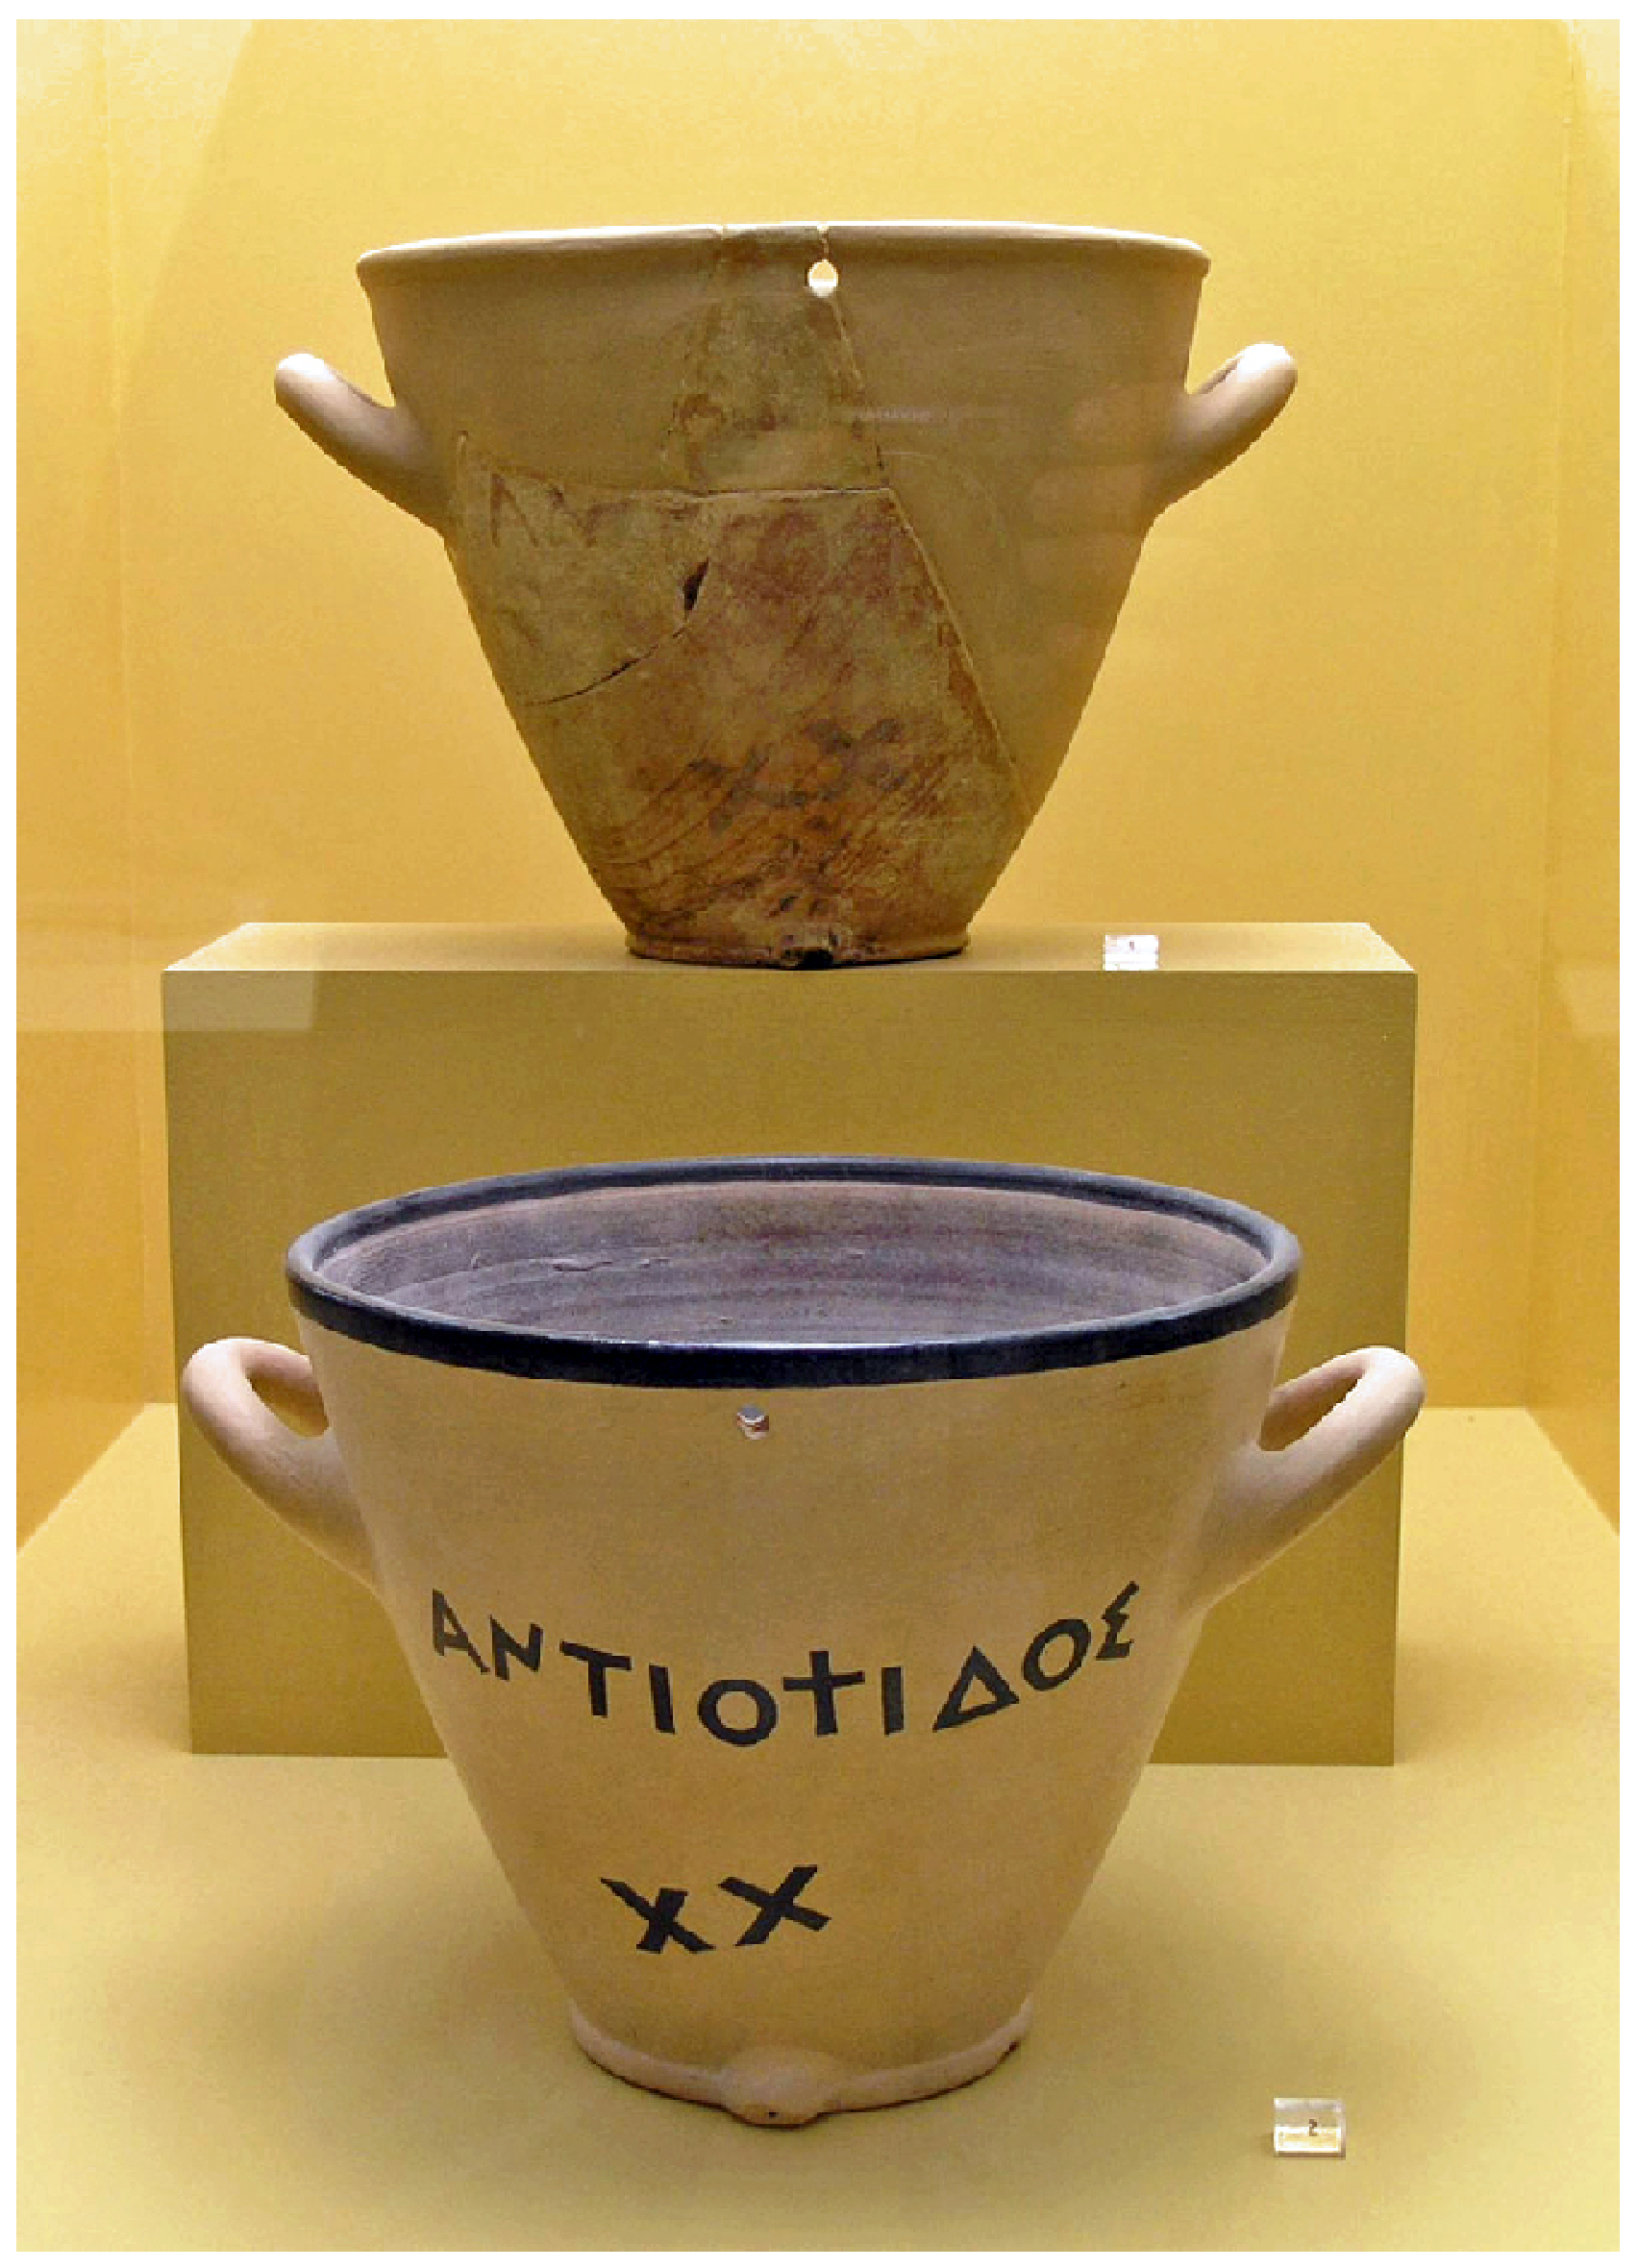
\includegraphics[width=0.45\linewidth,height=10cm]{fig/AGMA_Clepsydre_m.eps}
%\label{fig-clep}
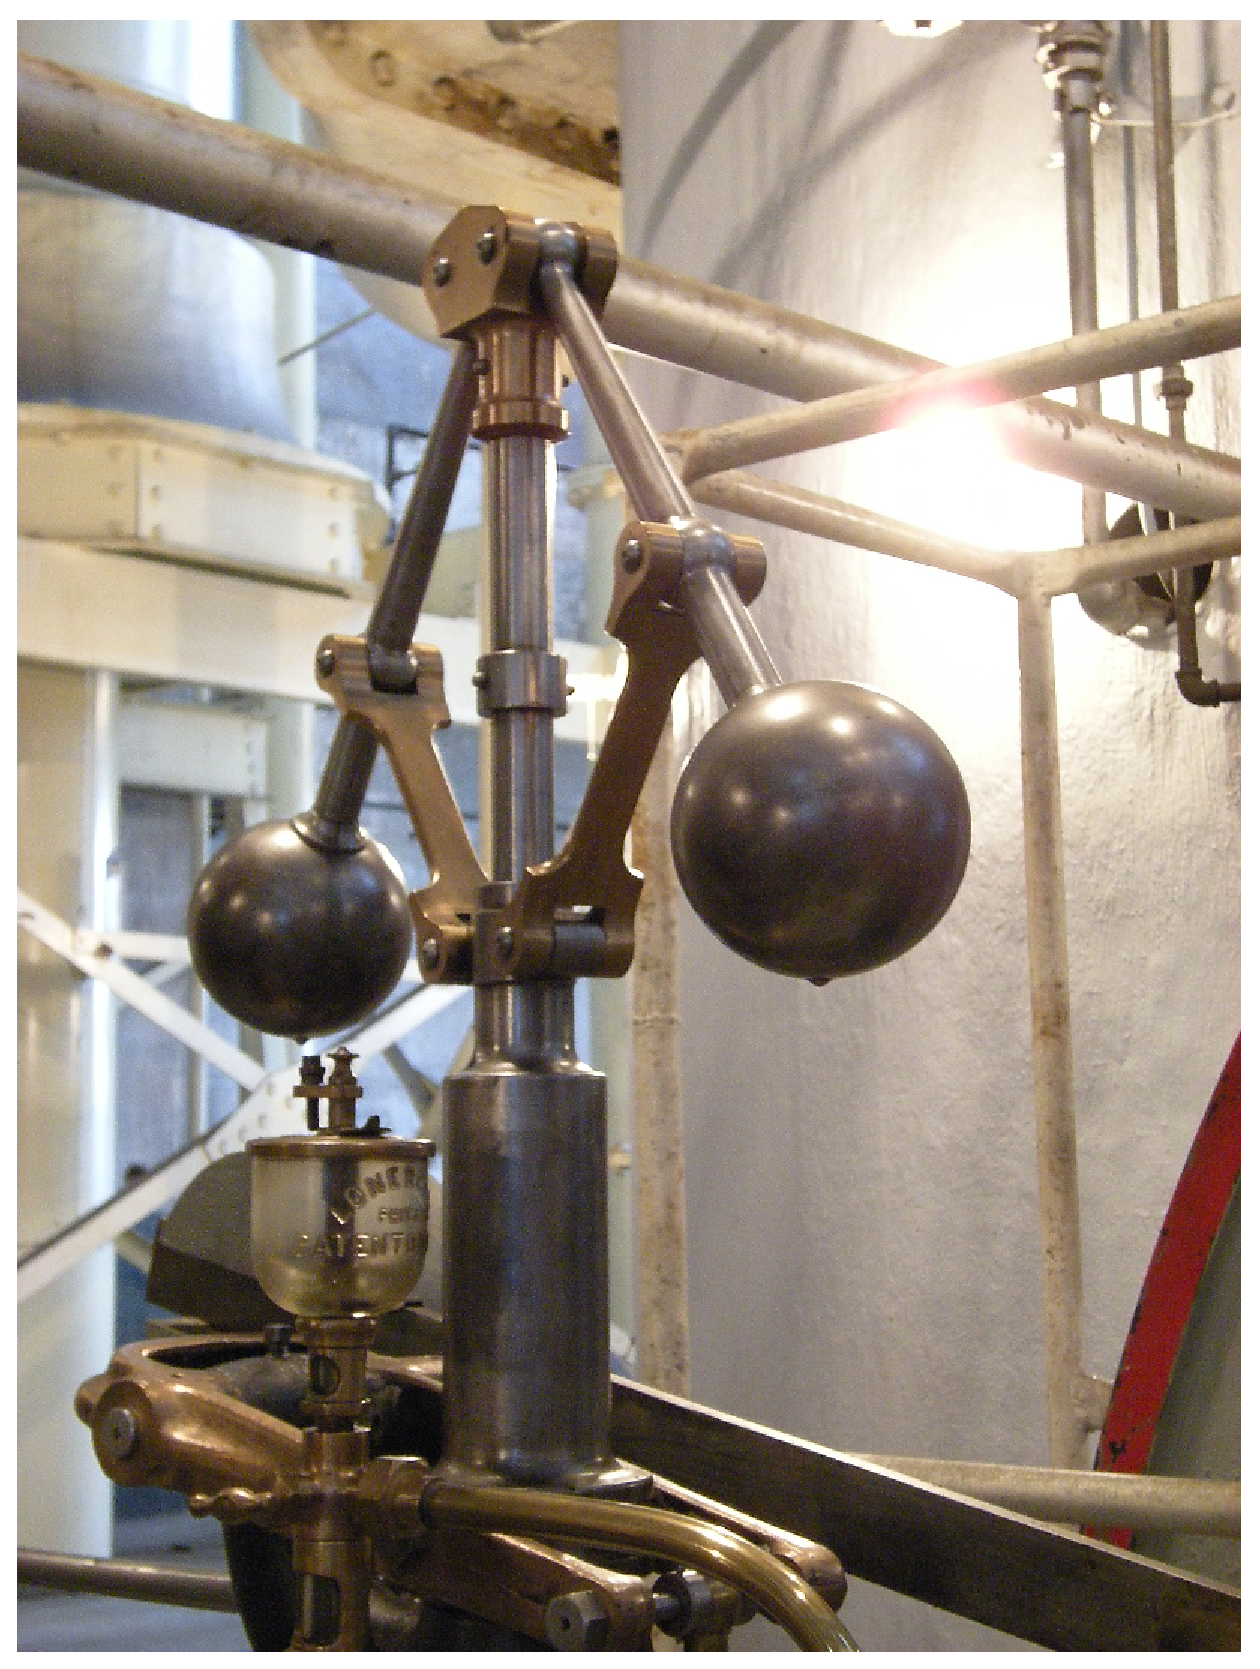
\includegraphics[width=0.45\linewidth,height=10cm]
{fig/Georgetown_PowerPlant_Museum_m.eps}
%\label{fig-watt}
%\caption{Exemples historiques de régulateur : 
%(gauche) Clepsydre athénienne (d'après \cite{clep}) 
%(droite) Régulateur de vitesse de Watt (d'après \cite{watt})\label{fig-hist}}
\caption{Exemple historique de régulateur : Régulateur 
de vitesse de Watt (d'après \cite{watt})\label{fig-hist}}
\end{figure}

Les chapitres précédents nous ont permis de caractériser, modéliser et
analyser la réponse temporelle des systèmes linéaires.
Nous allons maintenant aborder la possibilité du \textbf{contrôle} de ces 
systèmes par l'intermédiaire de l'\textbf{asservissement} et de 
\textbf{régulation}. 
L'idée sous-jacente est de permettre le contrôle automatique d'un système
sans l'intervention d'un opérateur humain dans l'établissement d'une commande
d'un système. 

La figure~\ref{fig-hist} montre un exemple historique de 
régulateur de vitesse ( également connu comme le régulateur à boules de Watt). 
La particularité de ce régulateur est d'avoir était utilisé dans l'industrie
du 18ème siècle bien avant les premières avancées théoriques dans le domaine 
de l'automatique. Dans le contexte des premières machines à vapeurs, 
il était important de contrôler la vitesse angulaire des turbines à vapeur. 
Le mécanisme de Watt permet avec un dispositif de retroaction d'agir sur la 
valve d'arrivée de la vapeur en fonction de la vitesse de l'axe de la turbine.

En effet, jusqu'à présent nous nous sommes intéressés à l'étude de système 
linéaire \og isolé\fg (de fonction de transfert $H(p)$) 
qui pour une entrée $E(p)$, élaborait une sortie $S(p)$\footnote{On conserve 
la représentation dans le domaine de Laplace de nos systèmes linéaires et 
des signaux mis en jeu physiquement dans le domaine temporel}.

\begin{center}
%\tikzsetnextfilename{sb_bloc0-chap5_ext}
\begin{tikzpicture}
    \sbEntree{E1}
	\sbBloc[3]{B1}{$H(p)$}{E1}
        \sbRelier[$E(p)$]{E1}{B1}
    \sbSortie[3]{S1}{B1}
        \sbRelier[$S(p)$]{B1}{S1}
\end{tikzpicture}
\end{center}

Nous avons pu caractériser la sortie en fonction de différentes 
performances: rapidité, précision, stabilité et dépassement. 
La question est de savoir maintenant comment agir sur le 
signal $E(p)$ pour contrôler la sortie $S(p)$ en fonction de critères
de performances choisis initialement.

Il existe deux approches pour élaborer la commande 
d'un système linéaire soit en boucle ouverte ou en boucle fermée.

\begin{itemize}
    \item En \textbf{boucle ouverte}: on place un correcteur $C(p)$
          en amont du système pour élaborer 
          la commande (que nous noterons $U(p)$) du système que l'on 
          souhaite contrôler. \`A noter que l'entrée du système appelée 
          dans le cadre de l'asservissement consigne est maintenant 
          l'entrée du correcteur.

\begin{center}
%\tikzsetnextfilename{sb_bloc1-chap5_ext}
\begin{tikzpicture}
    \sbEntree{E}
	\sbBloc[3]{C}{$C(p)$}{E}
    \sbRelier[$E(p)$]{E}{C}
	\sbBloc[3]{H}{$H(p)$}{C}
    \sbRelier[$U(p)$]{C}{H}
    \sbSortie[3]{S}{H}
    \sbRelier[$S(p)$]{H}{S}
    \node[yshift=-0.8em] at (C.south) {\small Correcteur};
    \node[yshift=-0.8em] at (H.south) {\small Système};
\end{tikzpicture}
\end{center}

    \item En \textbf{boucle fermée}: le principe consiste à mesurer le signal 
          de sortie pour ajuster le signal de commande. Pour celà, on place le
          système (corrigée ou non) dans une boucle de contre-réaction 
          \cref{chap-schemabloc}.

\begin{center}
%\tikzsetnextfilename{sb_bloc2-chap5_ext}
\begin{tikzpicture}
    \sbEntree{E}
	\sbComp{comp1}{E}
	\sbRelier[$E(p)$]{E}{comp1}
	\sbBloc[3]{C}{$C(p)$}{comp1}
    \sbRelier[$\epsilon(p)$]{comp1}{C}
	\sbBloc[3]{H}{$H(p)$}{C}
    \sbRelier[$U(p)$]{C}{H}
    \sbSortie[3]{S}{H}
    \sbRelier[$S(p)$]{H}{S}
	\sbRenvoi{H-S}{comp1}{}
    \node[yshift=-0.8em] at (C.south) {\small Correcteur};
    \node[yshift=-0.8em] at (H.south) {\small Système};
\end{tikzpicture}
\end{center}

\end{itemize}

%En d'autre mot, 
%Dans un sens, le signal $e(t)$ est la commande du système 
%De tel système

La \textbf{régulation} consiste à contrôler la sortie d'un système
pour une consigne fixe quelque soit les perturbations variables au 
cours du temps.

L'\textbf{asservissement} consiste à suivre une consigne variable 
au cours du temps.

%Imaginons que l'on souhaite étudier la température de l'eau 
%fournie par une douche. 

%Dans ce chapitre, nous allons aborder la notion d'asservissement des 
%systèmes linéaires que nous avons maitenant caractérisé, modélisisé et
%analysé dans les chapitres précédents.
%L'idée d'asservissement 


\clearpage
%%%%%%%%%%%%%%%%%%%%%%%%%%%%%%%%%%%%%%%%%%%%%%%%%%%%%%%%%%%%%%%%%%%%%%%%%%%%%%%%
%%%%%%%%%%%%%%%%%%%%%%%%%%%%%%%%%%%%%%%%%%%%%%%%%%%%%%%%%%%%%%%%%%%%%%%%%%%%%%%%
%%%%%%%%%%%%%%%%%%%%%%%%%%%%%%%%%%%%%%%%%%%%%%%%%%%%%%%%%%%%%%%%%%%%%%%%%%%%%%%%
\section{Organisation d'un asservissement}
%%%%%%%%%%%%%%%%%%%%%%%%%%%%%%%%%%%%%%%%%%%%%%%%%%%%%%%%%%%%%%%%%%%%%%%%%%%%%%%%
%%%%%%%%%%%%%%%%%%%%%%%%%%%%%%%%%%%%%%%%%%%%%%%%%%%%%%%%%%%%%%%%%%%%%%%%%%%%%%%%
%%%%%%%%%%%%%%%%%%%%%%%%%%%%%%%%%%%%%%%%%%%%%%%%%%%%%%%%%%%%%%%%%%%%%%%%%%%%%%%%

%%%%%%%%%%%%%%%%%%%%%%%%%%%%%%%%%%%%%%%%%%%%%%%%%%%%%%%%%%%%%%%%%%%%%%%%%%%%%%%%
%%%%%%%%%%%%%%%%%%%%%%%%%%%%%%%%%%%%%%%%%%%%%%%%%%%%%%%%%%%%%%%%%%%%%%%%%%%%%%%%
\subsection{Schémas fonctionnels associés aux systèmes asservis}
%%%%%%%%%%%%%%%%%%%%%%%%%%%%%%%%%%%%%%%%%%%%%%%%%%%%%%%%%%%%%%%%%%%%%%%%%%%%%%%%
%%%%%%%%%%%%%%%%%%%%%%%%%%%%%%%%%%%%%%%%%%%%%%%%%%%%%%%%%%%%%%%%%%%%%%%%%%%%%%%%

\begin{figure}[!h]
%%%%%%%%%%%%%%%%%%%%%%%%%%%%%%%%%%%%%%%%%%%%%%%%%%%%%%%%%%%%%%%%%%%%%%%%%%%%%%%%
%   Nom des noeuds
%                                      
%   E ---- a ---- b ---- c ---- S
%          |                |
%          |                |
%            ---- d ------- 
% E : entrée
% a : comparateur
% b : correcteur
% c : système
% S : sortie
% d : capteur
% r : noeud décalé pour le retour
%%%%%%%%%%%%%%%%%%%%%%%%%%%%%%%%%%%%%%%%%%%%%%%%%%%%%%%%%%%%%%%%%%%%%%%%%%%%%%%%
%\begin{center}
%    \begin{tikzpicture}
%        \sbEntree{E}
%        \sbComp{a}{E}
%        \sbRelier[$E(p)$]{E}{a}           % entree
%        \sbBloc[3]{b}{$C(p)$}{a}
%        \sbRelier[$\epsilon(p)$]{a}{b}    % ecart
%        \sbBloc[3]{c}{$H(p)$}{b}
%        \sbRelier[$U(p)$]{b}{c}           % commande
%        \sbSortie[4]{S}{c}
%        \sbRelier{c}{S}
%        \sbNomLien[0.8]{S}{$S(p)$}
%        \sbDecaleNoeudy[6]{b-c}{r}
%        \sbBlocr[-1.6]{d}{$G(p)$}{r}
%        \sbRelieryx{c-S}{d}              
%        \sbRelierxy[$M(p)$]{d}{a}         % mesure (image de S)
%        \node[yshift=-0.8em] at (b.south) {\small Correcteur};
%        \node[yshift=-0.8em] at (c.south) {\small Système};
%        \node[yshift=-0.8em] at (d.south) {\small Capteur};
%        \node[yshift=-0.8em,xshift=0.5em] at (E.south) {\small Consigne};
%        \node[yshift=-0.8em] at (S.south) {\small Sortie};
%    \end{tikzpicture}
%\end{center}

%avec cadre régulateur
    \begin{center}
    \tikzsetnextfilename{reg_1-chap4_ext}
        \begin{tikzpicture}
            \sbEntree{E}
            \sbComp{a}{E}
            \sbRelier[$E(p)$]{E}{a}           % entree
            \sbBloc[3]{b}{$C(p)$}{a}
            \sbRelier[$\epsilon(p)$]{a}{b}    % ecart
            \sbBloc[4.2]{c}{$H(p)$}{b}
            \sbRelier[$U(p)$]{b}{c}           % commande
            \sbSortie[4]{S}{c}
            \sbRelier{c}{S}
            \sbNomLien[0.8]{S}{$S(p)$}
            \sbDecaleNoeudy[7]{b-c}{r}
            \sbBlocr[-1.6]{d}{$G(p)$}{r}
            \sbRelieryx{c-S}{d}              
            \sbRelierxy[$M(p)$]{d}{a}         % mesure (image de S)
            \node[yshift=-0.8em] at (b.south) {\small Correcteur};
            \node[yshift=-0.8em] at (c.south) {\small Système};
            \node[yshift=-0.8em] at (d.south) {\small Capteur};
            \draw[dashed,very thick,blue] (1.15,-1.8) rectangle 
            node[blue,xshift=-1.9em,yshift=4em] {\textbf{Régulateur}} (4.9,1);
            \node[yshift=-0.8em,xshift=0.5em] at (E.south) {\small Consigne};
            \node[yshift=-0.8em] at (S.south) {\small Sortie};
        \end{tikzpicture}
    \end{center}
    \caption{Schéma fonctionnel classique de l'asservissement d'un système 
             présentant un correcteur et un capteur.\label{fig-reg}}
\end{figure}

%%%%%%%%%%%%%%%%%%%%%%%%%%%%%%%%%%%%%%%%%%%%%%%%%%%%%%%%%%%%%%%%%%%%%%%%%%%%%%%%
%   Nom des noeuds
%                                      
%                                      
%   E ---- a ---- b ---- c ---- d ---- e ---- S
%                 |                       |
%                 |                       |
%                  --------- f -----------
% E : entrée
% a : adaptateur 
% b : comparateur
% c : correcteur
% d : actionneur
% e : système
% S : sortie
% f : capteur
% r : noeud décalé pour le retour
%%%%%%%%%%%%%%%%%%%%%%%%%%%%%%%%%%%%%%%%%%%%%%%%%%%%%%%%%%%%%%%%%%%%%%%%%%%%%%%%
%\begin{center}
%    \begin{tikzpicture}
%        \sbEntree{E}
%        \sbBloc[3]{a}{$A_d(p)$}{E}
%        \sbRelier[$E(p)$]{E}{a}
%        \sbComp{b}{a}
%        \sbRelier{a}{b}
%        \sbBloc[3]{c}{$C(p)$}{b}
%        \sbRelier[$\epsilon(p)$]{b}{c}
%        \sbBloc[3]{d}{$A_c(p)$}{c}
%        \sbRelier[$\epsilon'(p)$]{c}{d}
%        \sbBloc[3]{e}{$H(p)$}{d}
%        \sbRelier[$U(p)$]{d}{e}
%        \sbSortie[4]{S}{e}
%        \sbRelier{e}{S}
%        \sbDecaleNoeudy[5]{d}{r}
%        \sbBlocr[-1.6]{f}{$G(p)$}{r}
%        \sbRelieryx{e-S}{f}              
%        \sbRelierxy[$M(p)$]{f}{b}        % Mesure
%        \sbNomLien[0.8]{S}{$S(p)$}
%        \node[yshift=-0.8em] at (a.south) {\small Adaptateur};
%        \node[yshift=-0.8em] at (c.south) {\small Correcteur};
%        \node[yshift=-0.8em] at (d.south) {\small Actionneur};
%        \node[yshift=-0.8em] at (e.south) {\small Système};
%        \node[yshift=-0.8em] at (f.south) {\small Capteur};
%        \node[yshift=-0.8em,xshift=0.5em] at (E.south) {\small Consigne};
%        \node[yshift=-0.8em] at (S.south) {\small Sortie};
%    \end{tikzpicture}
%\end{center}

%%%%%%%%%%%%%%%%%%%%%%%%%%%%%%%%%%%%%%%%%%%%%%%%%%%%%%%%%%%%%%%%%%%%%%%%%%%%%%%%
%   Nom des noeuds
%                                      P
%                                      |
%                                      |
%   E ---- a ---- b ---- c ---- d ---- e ---- f ---- S
%                 |                              |
%                 |                              |
%                  ------------ g ---------------
% E : entrée
% a : adaptateur 
% b : comparateur
% c : correcteur
% d : actionneur
% e : sommateur (perturbation)
% P : perturbation
% f : système 
% S : sortie
% g : capteur
% r : noeud décalé pour le retour
%%%%%%%%%%%%%%%%%%%%%%%%%%%%%%%%%%%%%%%%%%%%%%%%%%%%%%%%%%%%%%%%%%%%%%%%%%%%%%%%
%\begin{landscape}
%\vspace*{\fill}
\begin{center}
\tikzsetnextfilename{asser-chap4_ext}
    \begin{tikzpicture}
        \sbEntree{E}
        \sbBloc[3]{a}{$A_d(p)$}{E}
        \sbRelier[$E(p)$]{E}{a}
        \sbComp{b}{a}
        \sbRelier{a}{b}
        \sbBloc[3]{c}{$C(p)$}{b}
        \sbRelier[$\epsilon(p)$]{b}{c}
        \sbBloc[3]{d}{$A_c(p)$}{c}
%        \sbRelier[$\epsilon'(p)$]{c}{d}
        \sbRelier{c}{d}
        \sbSumh[6.7]{e}{d}
        \sbDecaleNoeudy[-3]{e}{P}
        \sbRenvoiF[-3]{P}{e}{$P(p)$}
        \sbRelier[$U(p)$]{d}{e}
        \sbBloc{f}{$H(p)$}{e}
        \sbRelier{e}{f}
        \sbSortie[4]{S}{f}
        \sbRelier{f}{S}
        \sbDecaleNoeudy[5]{c}{r}
        \sbBlocr[-1.6]{g}{$G(p)$}{r}
        \sbRelieryx{f-S}{g}              
        \sbRelierxy[$M(p)$]{g}{b}        
        \sbNomLien[0.8]{S}{$S(p)$}
        \node[yshift=-0.8em] at (a.south) {\small Adaptateur};
        \node[yshift=-0.8em] at (c.south) {\small Correcteur};
        \node[yshift=-0.8em] at (d.south) {\small Actionneur};
        \node[yshift=-0.8em] at (f.south) {\small Système};
        \node[yshift=-0.8em] at (g.south) {\small Capteur};
        \node[yshift=-0.8em,xshift=0.5em] at (E.south) {\small Consigne};
        \node[yshift=-0.8em] at (S.south) {\small Sortie};
        \node[yshift=2em,xshift=2.8em] at (P.east) {\small Perturbation};
        \draw[dashed,very thick,blue](-0.8,-4) 
        rectangle node[blue,xshift=-3.2em,yshift=7em]
        {\textbf{Chaîne d'information}}(6.9,2.5);
        \draw[dashed,very thick,red](7.3,-4)
        rectangle node[red,xshift=-5.9em,yshift=7em]  
        {\textbf{Chaîne d'énergie}    }(15.9,2.5);
        \draw[very thick,green!50!black,dashed,-latex] (4,1)   -- 
        node[green!50!black,above] {Chaîne direct} (14,1) ;
        \draw[very thick,green!50!black,dashed,-latex] (14,-3.7) -- 
        node[green!50!black,above] {Chaîne de retour} (4,-3.7) ;
    \end{tikzpicture}
\end{center}
    \captionof{figure}{Décomposition en chaîne d'information et chaîne 
                       d'énergie d'un schéma bloc d'asservissement 
                       complet\label{fig-asser}}

\begin{table}[!h]
    \ra{1.5}
    \centering
    \begin{tabular}{@{}P{3cm}m{8.5cm}P{3cm}@{}}
        \toprule
Composants      & Description & Fonction de transfert ou signal associés\\
        \midrule
Consigne/Entrée & La valeur que l'on souhaite atteindre en sortie 
                  du système asservi. Cette consigne peut être constante 
                  ou dépendante du temps. 
                & $E(p)$                                                \\
Adaptateur      & Adapte le signal de consigne à l'image de la sortie.
                & $A_d(p)$                                              \\
Correcteur      & \'Elabore à partir du signal d'écart $\epsilon(p)$ 
                  la commande $U(p)$ ou la grandeur réglante du système.
                & $C(p)$                                                \\
Actionneur      & L'organe d'action qui apporte l'énergie au système.
                & $A_c(p)$                                              \\
Commande        & Le signal de commande du système élaboré par l'actionneur 
		                  ou le correcteur.
                & $U(p)$                                                \\
Système         & Le système que l'on souhaite contrôler et/ou asservir
                & $H(p)$                                                \\
Régulateur      & Le régulateur se compose d'un comparateur qui élabore le 
                  signal d'écart $\epsilon(p)$ à partir de la consigne et de 
                  la mesure, formellement le régulateur incorpore 
                  également le correcteur.
                & $\epsilon(p)$                                         \\
Perturbation    & Phénomène physique intervenant sur le système qui 
                  en modifie la sortie
                & $P(p)$                                                \\
Capteur         &  Le capteur prélève le sortie pour en donner une 
                   image (la mesure) utile au régulateur. 
                   Intervenant dans la boucle ouverte, son étude 
                   est indispensable pour la caractérisation des 
                   performances du système asservi.
                & $G(p)$                                                \\
Mesure          & Le signal de la mesure de la sortie ou image de la sortie
                  élaboré par le capteur.
                & $M(p)$                                                \\
Sortie          & Le signal de sortie du système que l'on souhaite 
                  régulé et/ou asservir.
                & $S(p)$                                                \\
        \bottomrule
    \end{tabular}
\caption{Terminologie et définition associés à l'asservissement des 
         systèmes.\label{tab-asser}}
\end{table}

\clearpage

%%%%%%%%%%%%%%%%%%%%%%%%%%%%%%%%%%%%%%%%%%%%%%%%%%%%%%%%%%%%%%%%%%%%%%%%%%%%%%%%
%%%%%%%%%%%%%%%%%%%%%%%%%%%%%%%%%%%%%%%%%%%%%%%%%%%%%%%%%%%%%%%%%%%%%%%%%%%%%%%%
\subsection{Fonctions de transferts associées à un système asservi}
%%%%%%%%%%%%%%%%%%%%%%%%%%%%%%%%%%%%%%%%%%%%%%%%%%%%%%%%%%%%%%%%%%%%%%%%%%%%%%%%
%%%%%%%%%%%%%%%%%%%%%%%%%%%%%%%%%%%%%%%%%%%%%%%%%%%%%%%%%%%%%%%%%%%%%%%%%%%%%%%%

Chacuns des blocs du schéma fonctionnel d'un asservissement~\cref{fig-asser} 
permet de définir une fonction de transfert reliant localement une entrée 
et une sortie.
Nous allons définir quelques fonctions de transferts fondamentales à 
l'étude d'un système asservis.

%%%%%%%%%%%%%%%%%%%%%%%%%%%%%%%%%%%%%%%%%%%%%%%%%%%%%%%%%%%%%%%%%%%%%%%%%%%%%%%%
\paragraph{Fonction de transfert de la chaîne directe}
%%%%%%%%%%%%%%%%%%%%%%%%%%%%%%%%%%%%%%%%%%%%%%%%%%%%%%%%%%%%%%%%%%%%%%%%%%%%%%%%

La~\gls{ftcd}, que nous noterons $H_{CD}(p)$ est liée à 
la chaîne d'action de l'asservissement. Elle lie la sortie $S(p)$ à 
l'écart $\epsilon(p)$. Formellement,
\begin{bequation}[ams align]
H_{CD}(p)=\dfrac{S(p)}{\epsilon(p)}
\end{bequation}

%%%%%%%%%%%%%%%%%%%%%%%%%%%%%%%%%%%%%%%%%%%%%%%%%%%%%%%%%%%%%%%%%%%%%%%%%%%%%%%%
\paragraph{Fonction de transfert de la chaîne de retour}
%%%%%%%%%%%%%%%%%%%%%%%%%%%%%%%%%%%%%%%%%%%%%%%%%%%%%%%%%%%%%%%%%%%%%%%%%%%%%%%%

La~\gls{ftcr}, que nous noterons $H_{CR}(p)$ est 
liée à la chaîne de mesure de l'asservissement. Elle lie l'image 
de la sortie $M(p)$ à la sortie $S(p)$. 
Elle correspond essentiellement au capteur.
Formellement,
\begin{bequation}[ams align]
H_{CR}(p)=\dfrac{M(p)}{S(p)}
\end{bequation}
Dans le cas d'un retour unitaire $H_{CR}(p)=1$, c'est à dire que la sortie est 
la consigne sont de même nature.

%%%%%%%%%%%%%%%%%%%%%%%%%%%%%%%%%%%%%%%%%%%%%%%%%%%%%%%%%%%%%%%%%%%%%%%%%%%%%%%%
\paragraph{Fonction de transfert en boucle ouverte}
%%%%%%%%%%%%%%%%%%%%%%%%%%%%%%%%%%%%%%%%%%%%%%%%%%%%%%%%%%%%%%%%%%%%%%%%%%%%%%%%

La~\gls{ftbo}, que nous noterons $H_{BO}(p)$ correspond
à la fonction de transfert du système non asservi. Elle lie l'image de la 
sortie $M(p)$ à l'écart $\epsilon(p)$. Formellement,
\begin{bequation}[ams align]
H_{BO}(p)=\dfrac{M(p)}{\epsilon(p)}=
\dfrac{M(p)}{S(p)}\dfrac{S(p)}{\epsilon(p)}=H_{CR}(p)H_{CD}(p)
\end{bequation}
Dans le cas d'un retour unitaire on obtient $H_{BO}(p)=H_{CD}(p)$

%%%%%%%%%%%%%%%%%%%%%%%%%%%%%%%%%%%%%%%%%%%%%%%%%%%%%%%%%%%%%%%%%%%%%%%%%%%%%%%%
\paragraph{Fonction de transfert en boucle fermée}
%%%%%%%%%%%%%%%%%%%%%%%%%%%%%%%%%%%%%%%%%%%%%%%%%%%%%%%%%%%%%%%%%%%%%%%%%%%%%%%%

La~\gls{ftbf}, que nous noterons $H_{BF}(p)$ correspond
explicitement à la fonction de transfert du système asservi. 
Elle lie la sortie du système $S(p)$ à la consigne $E(p)$. Formellement et en 
appliquant la réduction des schémas blocs (c.f~\cref{sec-boucle}),
\begin{bequation}[ams align]
H_{BF}(p)=\dfrac{S(p)}{E(p)}=\dfrac{H_{CD}(p)}{1+H_{CR}(p)H_{CD}(p)}=
\dfrac{H_{CD}(p)}{1+H_{BO}(p)}
\end{bequation}

Remarquons que dans le cas d'une boucle de contre réaction unitaire 
(c.a.d $H_{CR}(p)=1$), la~\gls{ftbf} se réduit à :
$$
H_{BF}(p)=\dfrac{H_{BO}(p)}{1+H_{BO}(p)}
$$

Dans le cas d'une contre réaction unitaire, la~\gls{ftbf} ne dépend 
que de la~\gls{ftbo}.


%%%%%%%%%%%%%%%%%%%%%%%%%%%%%%%%%%%%%%%%%%%%%%%%%%%%%%%%%%%%%%%%%%%%%%%%%%%%%%%%
%%%%%%%%%%%%%%%%%%%%%%%%%%%%%%%%%%%%%%%%%%%%%%%%%%%%%%%%%%%%%%%%%%%%%%%%%%%%%%%%
%%%%%%%%%%%%%%%%%%%%%%%%%%%%%%%%%%%%%%%%%%%%%%%%%%%%%%%%%%%%%%%%%%%%%%%%%%%%%%%%
\section{Asservissement des SLCI modèles}
%%%%%%%%%%%%%%%%%%%%%%%%%%%%%%%%%%%%%%%%%%%%%%%%%%%%%%%%%%%%%%%%%%%%%%%%%%%%%%%%
%%%%%%%%%%%%%%%%%%%%%%%%%%%%%%%%%%%%%%%%%%%%%%%%%%%%%%%%%%%%%%%%%%%%%%%%%%%%%%%%
%%%%%%%%%%%%%%%%%%%%%%%%%%%%%%%%%%%%%%%%%%%%%%%%%%%%%%%%%%%%%%%%%%%%%%%%%%%%%%%%

Dans cette partie, nous présentons les asservissements par boucle 
de contre-réaction unitaire par de systèmes modèles déjà introduits 
au~\cref{chap-model}. Nous pourrons dégager la règle générale suivante :
\textbf{l'ordre $n$ d'une fonction de transfert en boucle ouverte $H_{BO}(p)$
est conservé en boucle fermée par l'asservissement.}

%%%%%%%%%%%%%%%%%%%%%%%%%%%%%%%%%%%%%%%%%%%%%%%%%%%%%%%%%%%%%%%%%%%%%%%%%%%%%%%%
%%%%%%%%%%%%%%%%%%%%%%%%%%%%%%%%%%%%%%%%%%%%%%%%%%%%%%%%%%%%%%%%%%%%%%%%%%%%%%%%
\subsection{Asservissement d'un intégrateur}
%%%%%%%%%%%%%%%%%%%%%%%%%%%%%%%%%%%%%%%%%%%%%%%%%%%%%%%%%%%%%%%%%%%%%%%%%%%%%%%%
%%%%%%%%%%%%%%%%%%%%%%%%%%%%%%%%%%%%%%%%%%%%%%%%%%%%%%%%%%%%%%%%%%%%%%%%%%%%%%%%

Considérons un système intégrateur asservi et régi par le schéma-bloc suivant :
\begin{center}
\tikzsetnextfilename{asser_int-chap4_ext}
    \begin{tikzpicture}
        \sbEntree{E}
        \sbComp{a}{E}
        \sbRelier[$E(p)$]{E}{a}
       % \sbBloc{b}{$C(p)$}{a}
        \sbBloc{b}{$\dfrac{K}{p}$}{a}
        \sbRelier{a}{b}
        \sbSortie[4]{S}{b}
        \sbRelier{b}{S}
        \sbRenvoi{b-S}{a}{}
        \sbNomLien[0.8]{S}{$S(p)$}
    \end{tikzpicture}
\end{center}

La fonction de transfert en boucle ouverte $H_{BO}(p)$ est telle que :
$$
H_{BO}(p)=\dfrac{K}{p}
$$
avec $K$ le gain statique. 
La~\gls{ftbf} est alors donnée :
$$
H_{BF}(p)=\dfrac{H(p)}{1+H(p)}=\dfrac{K}{p+K}=\dfrac{1}{\tau_{BF} p+1}
$$
Remarquons qu'un intégrateur asservi devient un système du premier 
ordre de gain statique unité et de constante de temps $\tau_{BF}=\dfrac{1}{K}$ 
où $K$ est le gain statique de la~\gls{ftbo}\footnote{Un intégrateur étant 
un système du premier ordre particulier, nous avons bien l'ordre de $H_{BO}(p)$ 
qui est égal à l'ordre de $H_{BF}(p)$.}. 

Au~\cref{chap-model}, nous avons pu conclure que les systèmes du premier ordre 
sont fondamentalement stable (du moins pour $\tau>0$) et que les intégrateurs 
sont instables.
Ainsi, nous observons que \textbf{l'asservissement permet de stabiliser un 
système intrinsèquement instable.} 

%%%%%%%%%%%%%%%%%%%%%%%%%%%%%%%%%%%%%%%%%%%%%%%%%%%%%%%%%%%%%%%%%%%%%%%%%%%%%%%%
%%%%%%%%%%%%%%%%%%%%%%%%%%%%%%%%%%%%%%%%%%%%%%%%%%%%%%%%%%%%%%%%%%%%%%%%%%%%%%%%
\subsection{Asservissement d'un système du premier ordre}
%%%%%%%%%%%%%%%%%%%%%%%%%%%%%%%%%%%%%%%%%%%%%%%%%%%%%%%%%%%%%%%%%%%%%%%%%%%%%%%%
%%%%%%%%%%%%%%%%%%%%%%%%%%%%%%%%%%%%%%%%%%%%%%%%%%%%%%%%%%%%%%%%%%%%%%%%%%%%%%%%

Considérons un système du premier ordre asservi et régi par le schéma-bloc 
suivant :
\begin{center}
\tikzsetnextfilename{asser_1er-chap4_ext}
    \begin{tikzpicture}
        \sbEntree{E}
        \sbComp{a}{E}
        \sbRelier[$E(p)$]{E}{a}
       % \sbBloc{b}{$C(p)$}{a}
        \sbBloc{b}{$\dfrac{K}{1+\tau p}$}{a}
        \sbRelier{a}{b}
        \sbSortie[4]{S}{b}
        \sbRelier{b}{S}
        \sbRenvoi{b-S}{a}{}
        \sbNomLien[0.8]{S}{$S(p)$}
    \end{tikzpicture}
\end{center}
La fonction de transfert en boucle ouverte $H_{BO}(p)$ du procédé est alors 
tel que:
$$
H_{BO}(p)=\dfrac{K}{1+\tau p}
$$
où $K$ est le gain statique et $\tau$ la constante de temps 
du système en boucle ouverte. 
La~\gls{ftbf} est alors donnée :
$$
H_{BF}(p)=\dfrac{H(p)}{1+H(p)}=\dfrac{K}{(1+K)+\tau p}
$$
Remarquons que comme attendu la~\gls{ftbf} reste du premier ordre. 
Sous sa forme canonique cette fonction de transfert devient :
$$
H_{BF}(p)=\dfrac{\dfrac{K}{1+K}}{1+\dfrac{\tau}{1+K}p}
=\dfrac{K_{BF}}{1+\tau_{BF} p}
$$
où $K_{BF}$ est le gain statique et $\tau_{BF}$ la constante de temps du 
système boucle fermée. Par identification, on alors les rélations suivantes 
entre les paramètres du premier ordre de la~\gls{ftbo} et les paramètres du 
premier ordre de la~\gls{ftbf} :
\begin{align*}
       K_{BF}&=\dfrac{K}{1+K}\\
    \tau_{BF}&=\dfrac{\tau}{1+K}
\end{align*}

Constatons que le gain statique en boucle ouverte $K$ intervient 
dans la définition du gain statique $K_{BF}$ et de la constante de temps 
$\tau_{BF}$ en boucle fermée. Ainsi en modifiant le paramètre $K$, il est 
possible de jouer sur les deux paramètres régissant la boucle fermée.
Pour $K>0$, le domaine de définition des paramètres du système en boucle 
fermée sont  $K_{BF}\in[0,1[$ et  $\tau_{BF}\in]0,\tau]$

%%%%%%%%%%%%%%%%%%%%%%%%%%%%%%%%%%%%%%%%%%%%%%%%%%%%%%%%%%%%%%%%%%%%%%%%%%%%%%%%
%%%%%%%%%%%%%%%%%%%%%%%%%%%%%%%%%%%%%%%%%%%%%%%%%%%%%%%%%%%%%%%%%%%%%%%%%%%%%%%%
\subsection{Asservissement d'un système du second ordre}
%%%%%%%%%%%%%%%%%%%%%%%%%%%%%%%%%%%%%%%%%%%%%%%%%%%%%%%%%%%%%%%%%%%%%%%%%%%%%%%%
%%%%%%%%%%%%%%%%%%%%%%%%%%%%%%%%%%%%%%%%%%%%%%%%%%%%%%%%%%%%%%%%%%%%%%%%%%%%%%%%

Considérons un système du second ordre asservi et régi par le schéma-bloc 
suivant :
\begin{center}
\tikzsetnextfilename{asser_2nd-chap4_ext}
    \begin{tikzpicture}
        \sbEntree{E}
        \sbComp{a}{E}
        \sbRelier[$E(p)$]{E}{a}
       % \sbBloc{b}{$C(p)$}{a}
        \sbBloc{b}{$\dfrac{K\omega^2_0}{\omega^2_0+2\xi\omega_0p+p^2}$}{a}
        \sbRelier{a}{b}
        \sbSortie[4]{S}{b}
        \sbRelier{b}{S}
        \sbRenvoi{b-S}{a}{}
        \sbNomLien[0.8]{S}{$S(p)$}
    \end{tikzpicture}
\end{center}
La fonction de transfert en boucle ouverte du procédé $H_{BO}(p)$ est tel que:
$$
H_{BO}(p)=\dfrac{K\omega^2_0}{\omega^2_0+2\xi\omega_0p+p^2}
$$
où $K$ est le gain statique, $\omega_0$ la pulsation propre et $\xi$ 
le coefficient d'amortissement du système en boucle ouverte.
La~\gls{ftbf} est donnée par :
$$
H_{BF}(p)=\dfrac{H(p)}{1+H(p)}=
\dfrac{K\omega^2_0}{\omega^2_0(1+K)+2\xi\omega_0p+p^2}
$$
Une nouvelle fois, nous constatons que la fonction de transfert en 
boucle fermée est du même ordre que celle en boucle ouverte. 
Sous une forme canonique la~\gls{ftbf} devient :
$$
H_{BF}(p)=\dfrac{K\omega^2_0}{\omega^2_0(1+K)+2\xi\omega_0p+p^2}=
\dfrac{K_{BF}\omega^2_{0,BF}}{\omega^2_{0,BF}(1+K_{BF})+
2\xi_{BF}\omega_{0,BF}p+p^2}
$$
Par identification, on alors les rélations suivantes entre 
les paramètres du second ordre de la~\gls{ftbo} et les paramètres du 
second ordre de la~\gls{ftbf} :
\begin{align*}
       K_{BF}&=\dfrac{K}{1+K}\\
    \omega_{0,BF}&=\omega_0\sqrt{1+K}\\
    \xi_{BF}&=\dfrac{\xi}{\sqrt{1+K}}
\end{align*}

On remarque que influencer le gain de la boucle ouverte permet de modifier
tous les paramètres du second ordre de la boucle fermée.

%%%%%%%%%%%%%%%%%%%%%%%%%%%%%%%%%%%%%%%%%%%%%%%%%%%%%%%%%%%%%%%%%%%%%%%%%%%%%%%%
%%%%%%%%%%%%%%%%%%%%%%%%%%%%%%%%%%%%%%%%%%%%%%%%%%%%%%%%%%%%%%%%%%%%%%%%%%%%%%%%
%%%%%%%%%%%%%%%%%%%%%%%%%%%%%%%%%%%%%%%%%%%%%%%%%%%%%%%%%%%%%%%%%%%%%%%%%%%%%%%%
%\section{Performances des systèmes en boucle ouverte}
%%%%%%%%%%%%%%%%%%%%%%%%%%%%%%%%%%%%%%%%%%%%%%%%%%%%%%%%%%%%%%%%%%%%%%%%%%%%%%%%
%%%%%%%%%%%%%%%%%%%%%%%%%%%%%%%%%%%%%%%%%%%%%%%%%%%%%%%%%%%%%%%%%%%%%%%%%%%%%%%%
%%%%%%%%%%%%%%%%%%%%%%%%%%%%%%%%%%%%%%%%%%%%%%%%%%%%%%%%%%%%%%%%%%%%%%%%%%%%%%%%

%Nous regroupons ici les résultats 
%des performances des systèmes modèles étudiés au chapitre~\cref{chap-model}.
%Les critères sont établies de la façon suivante. de performances sont la 
%stabilité, la précision, la rapidité  
%et le dépassement.

%%%%%%%%%%%%%%%%%%%%%%%%%%%%%%%%%%%%%%%%%%%%%%%%%%%%%%%%%%%%%%%%%%%%%%%%%%%%%%%%
%\paragraph{1er ordre}
%%%%%%%%%%%%%%%%%%%%%%%%%%%%%%%%%%%%%%%%%%%%%%%%%%%%%%%%%%%%%%%%%%%%%%%%%%%%%%%%
%Le système est stable pour $\tau>0$.

%Le temps de réponse à 5\% est de $3\tau$

%Le système est précis pour $K=1$ puisque la valeur finale de la 
%réponse indicielle est de $KE_0$.


%%%%%%%%%%%%%%%%%%%%%%%%%%%%%%%%%%%%%%%%%%%%%%%%%%%%%%%%%%%%%%%%%%%%%%%%%%%%%%%%
%\paragraph{2nd ordre}
%%%%%%%%%%%%%%%%%%%%%%%%%%%%%%%%%%%%%%%%%%%%%%%%%%%%%%%%%%%%%%%%%%%%%%%%%%%%%%%%
%Le système est stable pour $\xi>0$.

%Le temps de réponse à 5\% est minimale pour $\xi\sim0.7$.

%Le système est précis pour $K=1$.
%
%Le système présente des dépassement pour $\xi<1$ 


%\newpage
%%%%%%%%%%%%%%%%%%%%%%%%%%%%%%%%%%%%%%%%%%%%%%%%%%%%%%%%%%%%%%%%%%%%%%%%%%%%%%%%
%%%%%%%%%%%%%%%%%%%%%%%%%%%%%%%%%%%%%%%%%%%%%%%%%%%%%%%%%%%%%%%%%%%%%%%%%%%%%%%%
%%%%%%%%%%%%%%%%%%%%%%%%%%%%%%%%%%%%%%%%%%%%%%%%%%%%%%%%%%%%%%%%%%%%%%%%%%%%%%%%
%\section*{Exercices du chapitre}
%%%%%%%%%%%%%%%%%%%%%%%%%%%%%%%%%%%%%%%%%%%%%%%%%%%%%%%%%%%%%%%%%%%%%%%%%%%%%%%%
%%%%%%%%%%%%%%%%%%%%%%%%%%%%%%%%%%%%%%%%%%%%%%%%%%%%%%%%%%%%%%%%%%%%%%%%%%%%%%%%
%%%%%%%%%%%%%%%%%%%%%%%%%%%%%%%%%%%%%%%%%%%%%%%%%%%%%%%%%%%%%%%%%%%%%%%%%%%%%%%%


%\exercice{}
%\question

%\newpage
%%%%%%%%%%%%%%%%%%%%%%%%%%%%%%%%%%%%%%%%%%%%%%%%%%%%%%%%%%%%%%%%%%%%%%%%%%%%%%%%
%%%%%%%%%%%%%%%%%%%%%%%%%%%%%%%%%%%%%%%%%%%%%%%%%%%%%%%%%%%%%%%%%%%%%%%%%%%%%%%%
%%%%%%%%%%%%%%%%%%%%%%%%%%%%%%%%%%%%%%%%%%%%%%%%%%%%%%%%%%%%%%%%%%%%%%%%%%%%%%%%
%\section*{Corrigé des exercices}
%%%%%%%%%%%%%%%%%%%%%%%%%%%%%%%%%%%%%%%%%%%%%%%%%%%%%%%%%%%%%%%%%%%%%%%%%%%%%%%%
%%%%%%%%%%%%%%%%%%%%%%%%%%%%%%%%%%%%%%%%%%%%%%%%%%%%%%%%%%%%%%%%%%%%%%%%%%%%%%%%
%%%%%%%%%%%%%%%%%%%%%%%%%%%%%%%%%%%%%%%%%%%%%%%%%%%%%%%%%%%%%%%%%%%%%%%%%%%%%%%%


%%%%%%%%%%%%%%%%%%%%%%%%%%%%%%%%%%%%%%%%%%%%%%%%%%%%%%%%%%%%%%%%%%%%%%%%%%%%%%%%
%%%%%%%%%%%%%%%%%%%%%%%%%%%%%%%%%%%%%%%%%%%%%%%%%%%%%%%%%%%%%%%%%%%%%%%%%%%%%%%%
%%%%%%%%%%%%%%%%%%%%%%%%%%%%%%%%%%%%%%%%%%%%%%%%%%%%%%%%%%%%%%%%%%%%%%%%%%%%%%%%
%%%%%%%%%%%%%%%%%%%%%%%%%%%%%%%%%%%%%%%%%%%%%%%%%%%%%%%%%%%%%%%%%%%%%%%%%%%%%%%%
%chap_asserv.tex
              %5 Asservissement
%%%%%%%%%%%%%%%%%%%%%%%%%%%%%%%%%%%%%%%%%%%%%%%%%%%%%%%%%%%%%%%%%%%%%%%%%%%%%%%%
%%%%%%%%%%%%%%%%%%%%%%%%%%%%%%%%%%%%%%%%%%%%%%%%%%%%%%%%%%%%%%%%%%%%%%%%%%%%%%%%
%%%%%%%%%%%%%%%%%%%%%%%%%%%%%%%%%%%%%%%%%%%%%%%%%%%%%%%%%%%%%%%%%%%%%%%%%%%%%%%%
%%%%%%%%%%%%%%%%%%%%%%%%%%%%%%%%%%%%%%%%%%%%%%%%%%%%%%%%%%%%%%%%%%%%%%%%%%%%%%%%
\chapter{Performances des systèmes asservis\label{chap-perf}}
%%%%%%%%%%%%%%%%%%%%%%%%%%%%%%%%%%%%%%%%%%%%%%%%%%%%%%%%%%%%%%%%%%%%%%%%%%%%%%%%
%%%%%%%%%%%%%%%%%%%%%%%%%%%%%%%%%%%%%%%%%%%%%%%%%%%%%%%%%%%%%%%%%%%%%%%%%%%%%%%%
%%%%%%%%%%%%%%%%%%%%%%%%%%%%%%%%%%%%%%%%%%%%%%%%%%%%%%%%%%%%%%%%%%%%%%%%%%%%%%%%
%%%%%%%%%%%%%%%%%%%%%%%%%%%%%%%%%%%%%%%%%%%%%%%%%%%%%%%%%%%%%%%%%%%%%%%%%%%%%%%%

\minitoc
\newpage

%%%%%%%%%%%%%%%%%%%%%%%%%%%%%%%%%%%%%%%%%%%%%%%%%%%%%%%%%%%%%%%%%%%%%%%%%%%%%%%%
%%%%%%%%%%%%%%%%%%%%%%%%%%%%%%%%%%%%%%%%%%%%%%%%%%%%%%%%%%%%%%%%%%%%%%%%%%%%%%%%
%%%%%%%%%%%%%%%%%%%%%%%%%%%%%%%%%%%%%%%%%%%%%%%%%%%%%%%%%%%%%%%%%%%%%%%%%%%%%%%%
\section{Contexte}
%%%%%%%%%%%%%%%%%%%%%%%%%%%%%%%%%%%%%%%%%%%%%%%%%%%%%%%%%%%%%%%%%%%%%%%%%%%%%%%%
%%%%%%%%%%%%%%%%%%%%%%%%%%%%%%%%%%%%%%%%%%%%%%%%%%%%%%%%%%%%%%%%%%%%%%%%%%%%%%%%
%%%%%%%%%%%%%%%%%%%%%%%%%%%%%%%%%%%%%%%%%%%%%%%%%%%%%%%%%%%%%%%%%%%%%%%%%%%%%%%%
Les performances qui vont nous interesser dans 
ce chapitre sont la \textbf{précision} et la \textbf{rapidité}

%%%%%%%%%%%%%%%%%%%%%%%%%%%%%%%%%%%%%%%%%%%%%%%%%%%%%%%%%%%%%%%%%%%%%%%%%%%%%%%%
%%%%%%%%%%%%%%%%%%%%%%%%%%%%%%%%%%%%%%%%%%%%%%%%%%%%%%%%%%%%%%%%%%%%%%%%%%%%%%%%
%%%%%%%%%%%%%%%%%%%%%%%%%%%%%%%%%%%%%%%%%%%%%%%%%%%%%%%%%%%%%%%%%%%%%%%%%%%%%%%%
\section{Précision}
%%%%%%%%%%%%%%%%%%%%%%%%%%%%%%%%%%%%%%%%%%%%%%%%%%%%%%%%%%%%%%%%%%%%%%%%%%%%%%%%
%%%%%%%%%%%%%%%%%%%%%%%%%%%%%%%%%%%%%%%%%%%%%%%%%%%%%%%%%%%%%%%%%%%%%%%%%%%%%%%%
%%%%%%%%%%%%%%%%%%%%%%%%%%%%%%%%%%%%%%%%%%%%%%%%%%%%%%%%%%%%%%%%%%%%%%%%%%%%%%%%
Un système est précis si l'écart que l'on note $\epsilon(t)$ 
entre l'entrée $e(t)$ et la sortie $s(t)$ est nul.
Dans le domaine de Laplace, cet écart devient :
$$
\epsilon(p)=E(p)-S(p)
$$

On distingue deux cas :
\begin{itemize}
    \item En régime permanent, cet écart $\epsilon_s$ est nommée 
		  \textbf{erreur statique. }
    \item En régime transitoire, cet écart $\epsilon(t)=e(t)-s(t)$ est 
		  nommée \textbf{erreur dynamique.}
\end{itemize}

L'erreur dynamique consiste à suivre l'écart défini précedemment durant 
le transitoire.

Pour étudier l'erreur statique, on sollicite le système à différents 
types de signaux pour obtenir dans les différents cas :
\begin{itemize}
	\item l'\textbf{erreur indicielle} ou l'erreur de position qui est 
		  l'erreur statique de la réponse indicielle.
	\item l'\textbf{erreur de poursuite} ou erreur de vitesse qui est 
		  l'erreur statique de la réponse à une rampe.
	\item l'\textbf{erreur en accélération} qui est l'erreur statique 
		  de la réponse à une parabole.
\end{itemize}
Concrétement pour étudier l'erreur statique on cherche la limite à l'infini 
de $\epsilon(t)$ ou encore en appliquant le théorème de la valeur finale :
\begin{bequation}[ams align]
\epsilon(\infty)=\lim\limits_{t\to\infty} e(t)-s(t)
	            =\lim\limits_{p\to 0} p\big(E(p)-S(p)\big)
\end{bequation}
Rappelons que pour pouvoir appliquer ce théorème la valeur finale doit 
être finie ou en d'autre mot le système doit être stable.

%%%%%%%%%%%%%%%%%%%%%%%%%%%%%%%%%%%%%%%%%%%%%%%%%%%%%%%%%%%%%%%%%%%%%%%%%%%%%%%%
%%%%%%%%%%%%%%%%%%%%%%%%%%%%%%%%%%%%%%%%%%%%%%%%%%%%%%%%%%%%%%%%%%%%%%%%%%%%%%%%
\subsection{Précision en boucle ouverte}
%%%%%%%%%%%%%%%%%%%%%%%%%%%%%%%%%%%%%%%%%%%%%%%%%%%%%%%%%%%%%%%%%%%%%%%%%%%%%%%%
%%%%%%%%%%%%%%%%%%%%%%%%%%%%%%%%%%%%%%%%%%%%%%%%%%%%%%%%%%%%%%%%%%%%%%%%%%%%%%%%

Soit un système caractérisé par la fonction de transfert $H(p)$ 
est sollicité par l'entrée $E(p)$. La sortie $S(p)$ est alors donnée par :

\begin{center}
\tikzsetnextfilename{sb_bloc1-chap6-ext}
\begin{tikzpicture}
    \sbEntree{E}
	\sbBloc[3]{H}{$H(p)$}{E}
    \sbRelier[$E(p)$]{E}{H}
    \sbSortie[3]{S}{H}
    \sbRelier[$S(p)$]{H}{S}
\end{tikzpicture}
\end{center}

L'erreur statique est alors donnée par :
$$
\epsilon(\infty)=\lim\limits_{p\to 0} p\big(E(p)-H(p)E(p)\big)
                =\lim\limits_{p\to 0} p\big(1-H(p)\big)E(p)
$$
%%%%%%%%%%%%%%%%%%%%%%%%%%%%%%%%%%%%%%%%%%%%%%%%%%%%%%%%%%%%%%%%%%%%%%%%%%%%%%%%
\subsubsection{Exemple d'un premier ordre}
%%%%%%%%%%%%%%%%%%%%%%%%%%%%%%%%%%%%%%%%%%%%%%%%%%%%%%%%%%%%%%%%%%%%%%%%%%%%%%%%
%Rappelons qu'il est possible de corriger la précision 
%d'un système en boucle ouverte. 
Prenons l'exemple d'un système du 1er ordre de fonction de transfert canonique 
$H(p)=\dfrac{K}{1+\tau p}$ que l'on sollicite avec un échelon 
d'amplitude (consigne) $E_0$.
L'erreur statique est alors donnée par :
$$
\epsilon(\infty)=\lim\limits_{p\to 0}\left(1-\dfrac{K}{1+\tau p}\right)E_0
                =(1-K)E_0
$$

Le système est prècis (c.a.d $\epsilon(\infty)=0$) si $K=1$. 

%Il alors possible de corriger en boucle ouverte la précision en 
%introduisant un gain $K'$ :

%\begin{center}
%\tikzsetnextfilename{sb_bloc2-chap6-ext}
%\begin{tikzpicture}
%    \sbEntree{E}
%	\sbBloc[3]{C}{$K'$}{E}
%    \sbRelier[$E(p)$]{E}{C}
%	\sbBloc[3]{H}{$\dfrac{K}{1+\tau p}$}{C}
%    \sbRelier[$U(p)$]{C}{H}
%    \sbSortie[3]{S}{H}
%    \sbRelier[$S(p)$]{H}{S}
%\end{tikzpicture}
%\end{center}
%tel que $K'K=1$ ou encore $K'=\frac{1}{K}$.

%Cependant, nous allons dans ce chapitre nous interesser uniquement 
% à l'asservissement en %boucle fermée.

%%%%%%%%%%%%%%%%%%%%%%%%%%%%%%%%%%%%%%%%%%%%%%%%%%%%%%%%%%%%%%%%%%%%%%%%%%%%%%%%
%%%%%%%%%%%%%%%%%%%%%%%%%%%%%%%%%%%%%%%%%%%%%%%%%%%%%%%%%%%%%%%%%%%%%%%%%%%%%%%%
\subsection{Précision en boucle fermée}
%%%%%%%%%%%%%%%%%%%%%%%%%%%%%%%%%%%%%%%%%%%%%%%%%%%%%%%%%%%%%%%%%%%%%%%%%%%%%%%%
%%%%%%%%%%%%%%%%%%%%%%%%%%%%%%%%%%%%%%%%%%%%%%%%%%%%%%%%%%%%%%%%%%%%%%%%%%%%%%%%

Considérons le cas d'un système asservi de fonction de transfert $H(p)$
par une boucle de contre-réaction à retour unitaire.

\begin{center}
\tikzsetnextfilename{sb_bloc3-chap6-ext}
\begin{tikzpicture}
    \sbEntree{E}
	\sbComp{comp1}{E}
	\sbRelier[$E(p)$]{E}{comp1}
	\sbBloc[3]{H}{$H(p)$}{comp1}
    \sbRelier[$\epsilon(p)$]{comp1}{H}
    \sbSortie[3]{S}{H}
    \sbRelier[$S(p)$]{H}{S}
	\sbRenvoi[4]{H-S}{comp1}{}
\end{tikzpicture}
\end{center}

La~\gls{ftbo} est simplement donnée par $H(p)$. Dans le cas le plus
générale, il est toujours possible d'écrire une fonction de transfert
sous la forme canonique (\Cref{chap-slci}) :
$$
H_{BO}(p)=\dfrac{K}{p^\alpha}\cdot\dfrac{N(p)}{D(p)}
$$
avec $\alpha$ la classe du système en boucle ouverte, $K$ le gain statique et 
$N(p)$ et $D(p)$ deux polynômes tels que $N(0)=D(0)=1$. 


Dans le domaine de Laplace l'écart $\epsilon(p)$ s'écrit :
$$
\epsilon(p)=E(p)-S(p)=\left(1-\dfrac{H_{BO}(p)}{1+H_{BO}(p)}\right)E(p)
$$
en remplaçant $H_{BO}(p)$ par sa représentation générale:
\begin{bequation}[ams align]
\epsilon(p)=\dfrac{p^\alpha D(p)}{p^\alpha D(p)+KN(p)}E(p)
\end{bequation}

L'erreur statique $\epsilon_s$ est alors donnée par la limite (Théorème 
de la valeur finale) :
$$
\epsilon_s=\lim\limits_{p\to 0} p\epsilon(p)=\lim\limits_{p\to 0} 
           \dfrac{p^\alpha D(p)}{p^\alpha D(p)+KN(p)}pE(p) 
$$
ou encore en utilisant les valeurs des polynômes en 0: 
\begin{bequation}[ams align]
	\epsilon_s=\lim\limits_{p\to 0} \dfrac{p^\alpha}{p^\alpha+K}pE(p)
	\label{eq-erreurStatique}
\end{bequation}

Cette erreur dépend donc de la nature de la sollicitation (c.a.d $E(p)$) et 
de la classe $\alpha$ de la fonction de transfert en boucle ouverte.

Nous allons maintenant considérer différentes types de sollicitations pour 
différentes classes de système en boucle ouverte.

%%%%%%%%%%%%%%%%%%%%%%%%%%%%%%%%%%%%%%%%%%%%%%%%%%%%%%%%%%%%%%%%%%%%%%%%%%%%%%%%
\subsubsection{Erreur statique indicielle}
%%%%%%%%%%%%%%%%%%%%%%%%%%%%%%%%%%%%%%%%%%%%%%%%%%%%%%%%%%%%%%%%%%%%%%%%%%%%%%%%

L'erreur indicielle est l'erreur entre la sortie d'un système et une 
sollicitation en échelon $e(t)=E_0u(t)$ de transformée de Laplace 
$E(p)=\dfrac{E_0}{p}$. 
Pour une telle entrée, l'erreur statique (c.f \cref{eq-erreurStatique}) 
devient :
$$
\epsilon_s=\lim\limits_{p\to 0} \dfrac{p^\alpha}{p^\alpha+K}E_0
$$

Dans le cas d'un système de classe $\alpha=0$ en boucle ouverte :
$$
\epsilon_s=\lim\limits_{p\to 0} \dfrac{p^0}{p^0+K}E_0=\dfrac{E_0}{1+K}.
$$
L'erreur est finie mais les réponses indicielles des systèmes de classe 
$\alpha=0$ en boucle ouverte ne sont pas précis.

Dans les autres cas $\alpha>0$, l'erreur statique s'annule :
$$
\epsilon_s=\lim\limits_{p\to 0} \dfrac{p^\alpha}{p^\alpha+K}E_0=0
$$
Les réponses indicielle des systèmes de classe $\alpha>0$ sont donc précis.

%%%%%%%%%%%%%%%%%%%%%%%%%%%%%%%%%%%%%%%%%%%%%%%%%%%%%%%%%%%%%%%%%%%%%%%%%%%%%%%%
\subsubsection{Erreur statique de poursuite}
%%%%%%%%%%%%%%%%%%%%%%%%%%%%%%%%%%%%%%%%%%%%%%%%%%%%%%%%%%%%%%%%%%%%%%%%%%%%%%%%
L'erreur de poursuite est l'erreur statique d'un système soumis à une rampe 
du type $e(t)=r(t)=E_0t u(t)$
de transformée de Laplace $E(p)=\dfrac{E_0}{p^2}$

Pour une telle entrée, l'erreur statique devient :
$$
\epsilon_s=\lim\limits_{p\to 0} \dfrac{p^\alpha}{p^\alpha+K}\dfrac{E_0}{p}
          =\dfrac{p^{\alpha-1}}{p^\alpha+K}E_0 
$$

Dans le cas d'un système de classe $\alpha=0$ en boucle ouverte, 
l'erreur devient :
$$
\epsilon_s=\lim\limits_{p\to 0}\dfrac{p^{-1}}{p^0+K}E_0=+\infty
$$
Le système est incapable de suivre l'entrée souhaitée.

Dans le cas d'un système de classe $\alpha=1$ en boucle ouverte, 
l'erreur devient :
$$
\epsilon_s=\lim\limits_{p\to 0}\dfrac{p^0}{p+K}E_0=\dfrac{E_0}{K}
$$

Dans le cas d'un système de classe $\alpha>1$ en boucle ouverte, 
l'erreur devient :
$$
\epsilon_s=\lim\limits_{p\to 0}\dfrac{p^{\alpha-1}}{p^\alpha+K}E_0=0
$$
Le système est donc prècis.

%%%%%%%%%%%%%%%%%%%%%%%%%%%%%%%%%%%%%%%%%%%%%%%%%%%%%%%%%%%%%%%%%%%%%%%%%%%%%%%%
\subsubsection{Erreur statique d'accélération}
%%%%%%%%%%%%%%%%%%%%%%%%%%%%%%%%%%%%%%%%%%%%%%%%%%%%%%%%%%%%%%%%%%%%%%%%%%%%%%%%

L'erreur d'accélération est l'erreur statique d'un système soumis à un signal
parabolique $e(t)=E_0t^2 u(t)$ de transformée de Laplace 
$E(p)=\dfrac{2E_0}{p^3}$

Pour une telle entrée, l'erreur statique devient :
$$
\epsilon_s=\lim\limits_{p\to 0} \dfrac{p^\alpha}{p^\alpha+K}\dfrac{2E_0}{p^2}
          =\dfrac{p^{\alpha-2}}{p^\alpha+K}2E_0 
$$

Dans le cas d'un système de classe $\alpha<2$ en boucle ouverte, 
l'erreur devient :
$$
\epsilon_s=+\infty
$$

Pour un système de classe $\alpha=2$ en boucle ouverte, 
l'erreur est finie :
$$
\epsilon_s=\dfrac{2E_0}{K}
$$
et s'annule pour $\alpha>2$

\begin{table}
    \ra{2.0}
    \centering
    \begin{tabular}{@{}P{2cm}P{2cm}P{2cm}P{2cm}P{2cm}@{}}
    \toprule
    Entrée & $\alpha=0$ & $\alpha=1$ & $\alpha=2$ & $\alpha>2$ \\
    \midrule
    $\dfrac{E_0}{p}$&$\dfrac{E_0}{1+K}$&0&0&0\\
    $\dfrac{E_0}{p^2}$&$+\infty$&$\dfrac{E_0}{K}$&0&0\\
    $\dfrac{2E_0}{p^3}$&$+\infty$&$+\infty$&$\dfrac{2E_0}{K}$&0\\
    \bottomrule
    \end{tabular}
\caption{Résumé des erreurs statiques pour différentes 
         sollicitations et classe de système en boucle ouverte}
\end{table}

%%%%%%%%%%%%%%%%%%%%%%%%%%%%%%%%%%%%%%%%%%%%%%%%%%%%%%%%%%%%%%%%%%%%%%%%%%%%%%%%
%%%%%%%%%%%%%%%%%%%%%%%%%%%%%%%%%%%%%%%%%%%%%%%%%%%%%%%%%%%%%%%%%%%%%%%%%%%%%%%%
\subsection{Effet d'une perturbation}
%%%%%%%%%%%%%%%%%%%%%%%%%%%%%%%%%%%%%%%%%%%%%%%%%%%%%%%%%%%%%%%%%%%%%%%%%%%%%%%%
%%%%%%%%%%%%%%%%%%%%%%%%%%%%%%%%%%%%%%%%%%%%%%%%%%%%%%%%%%%%%%%%%%%%%%%%%%%%%%%%
On considère maintenant l'effet d'une perturbation sur la précision d'un 
système asservis.
Sans perte de généralité, on ne considèrera que le cas d'une perturbation 
en entrée (c'est à dire en amont d'un système linéaire défini par une fonction 
de transfert $H_2(p)$, la présence d'un correcteur $H_1(p)$ n'est pas 
obligatoire mais facilite l'interprétation des résultats.

Considérons le schéma bloc suivant avec les fonctions de transfert $H_1(p)$ 
et $H_2(p)$ de forme canonique :
\begin{align*}
    H_1(p)=\dfrac{K_1}{p^{\alpha_1}}\dfrac{N_1(p)}{D_1(p)} \\
    H_2(p)=\dfrac{K_2}{p^{\alpha_2}}\dfrac{N_2(p)}{D_2(p)}
\end{align*}
de les gains statiques $K_i$, de classe $\alpha_i$, de polynômes $N_i(p)$
et $D_i(p)$ tels que $N_i(0)=$ et $D_i(0)=0$.

\begin{center}
\tikzsetnextfilename{reduc_mult1-chap6-ext}
\begin{tikzpicture}
    \cpbruni[$E(p)$]
        [$\epsilon(p)$]
        [$H_1(p)$]
        []
        [ ]
        [$P(p)$]
        [$H_2(p)$]
        []
        [$S(p)$]
\end{tikzpicture}
\end{center}

Pour déterminer l'écart à la consigne d'un tel système, il faut déterminer
la sortie globale du système asservis à deux entrées 
(c.f~\cref{chap_bloc}~\cref{sec-bloc_multE}).

%%%%%%%%%%%%%%%%%%%%%%%%%%%%%%%%%%%%%%%%%%%%%%%%%%%%%%%%%%%%%%%%%%%%%%%%%%%%%%%%
%%%%%%%%%%%%%%%%%%%%%%%%%%%%%%%%%%%%%%%%%%%%%%%%%%%%%%%%%%%%%%%%%%%%%%%%%%%%%%%%
%%%%%%%%%%%%%%%%%%%%%%%%%%%%%%%%%%%%%%%%%%%%%%%%%%%%%%%%%%%%%%%%%%%%%%%%%%%%%%%%
\section{Rapidité}
%%%%%%%%%%%%%%%%%%%%%%%%%%%%%%%%%%%%%%%%%%%%%%%%%%%%%%%%%%%%%%%%%%%%%%%%%%%%%%%%
%%%%%%%%%%%%%%%%%%%%%%%%%%%%%%%%%%%%%%%%%%%%%%%%%%%%%%%%%%%%%%%%%%%%%%%%%%%%%%%%
%%%%%%%%%%%%%%%%%%%%%%%%%%%%%%%%%%%%%%%%%%%%%%%%%%%%%%%%%%%%%%%%%%%%%%%%%%%%%%%%

%%%%%%%%%%%%%%%%%%%%%%%%%%%%%%%%%%%%%%%%%%%%%%%%%%%%%%%%%%%%%%%%%%%%%%%%%%%%%%%%
%%%%%%%%%%%%%%%%%%%%%%%%%%%%%%%%%%%%%%%%%%%%%%%%%%%%%%%%%%%%%%%%%%%%%%%%%%%%%%%%
\subsection{Réponse temporelle}
%%%%%%%%%%%%%%%%%%%%%%%%%%%%%%%%%%%%%%%%%%%%%%%%%%%%%%%%%%%%%%%%%%%%%%%%%%%%%%%%
%%%%%%%%%%%%%%%%%%%%%%%%%%%%%%%%%%%%%%%%%%%%%%%%%%%%%%%%%%%%%%%%%%%%%%%%%%%%%%%%

%%%%%%%%%%%%%%%%%%%%%%%%%%%%%%%%%%%%%%%%%%%%%%%%%%%%%%%%%%%%%%%%%%%%%%%%%%%%%%%%
%%%%%%%%%%%%%%%%%%%%%%%%%%%%%%%%%%%%%%%%%%%%%%%%%%%%%%%%%%%%%%%%%%%%%%%%%%%%%%%%
\subsection{Réponse harmonique}
%%%%%%%%%%%%%%%%%%%%%%%%%%%%%%%%%%%%%%%%%%%%%%%%%%%%%%%%%%%%%%%%%%%%%%%%%%%%%%%%
%%%%%%%%%%%%%%%%%%%%%%%%%%%%%%%%%%%%%%%%%%%%%%%%%%%%%%%%%%%%%%%%%%%%%%%%%%%%%%%%

%%%%%%%%%%%%%%%%%%%%%%%%%%%%%%%%%%%%%%%%%%%%%%%%%%%%%%%%%%%%%%%%%%%%%%%%%%%%%%%%
%%%%%%%%%%%%%%%%%%%%%%%%%%%%%%%%%%%%%%%%%%%%%%%%%%%%%%%%%%%%%%%%%%%%%%%%%%%%%%%%
\subsection{Influence des pôles dominants}
%%%%%%%%%%%%%%%%%%%%%%%%%%%%%%%%%%%%%%%%%%%%%%%%%%%%%%%%%%%%%%%%%%%%%%%%%%%%%%%%
%%%%%%%%%%%%%%%%%%%%%%%%%%%%%%%%%%%%%%%%%%%%%%%%%%%%%%%%%%%%%%%%%%%%%%%%%%%%%%%%

Soient $p_1,\ldots,p_n$ les pôles d'un système stable\footnote{À partir 
des résultats obtenus dans ce chapitre il est déjà clair que la stabilité
d'un système dépend également des pôles de sa fonction de transfert}.
Le pôle $p_i$ est dit dominant si la valeur absolue
de sa partie réelle est largement plus petite que celle de tout autre pôles 
du système\footnote{Dans la pratique un rapport de 5 est 
suffisant pour considérer une domination d'un pôle sur les autres}
\begin{bequation}[ams align]
    \big|\Re{p_i}\big| \ll \big|\Re{p_j}\big|\;\; \forall j\neq i
\end{bequation}

Pour observer l'influence d'un pôle dominant sur 
la réponse temporelle d'un système linéaire, nous
nous allons l'illustrer par l'étude d'une fonction 
de transfert du second ordre en régime apériodique.
Une telle fonction de transfert est équivalente à deux
systèmes du premier ordre en série.

Prenons l'exemple de la fonction de transfert définie par  
$$
H(p)=\dfrac{5}{(p+1)(5p+1)}
$$
et de décomposition en éléments simples telle que :
$$
H(p)=\dfrac{A}{p+1}+\dfrac{B}{5p+1}
$$
Par identification on peut écrire $H(p)$ en fonction de
deux fonctions de transferts $H_1(p)$ et $H_2(p)$ tel que :
\begin{align*}
	H(p)&=H_1(p)-H_2(p)\\
	H_1(p)&=\dfrac{6.25}{5p+1}\\
	H_2(p)&=\dfrac{1.25}{p+1}
\end{align*}

Par définition, le pôle dominant est donné par $H_1(p)$.
Pour observer son effet traçons les réponses indicielles 
de ces trois fonctions de transfert.

\begin{figure}[!h]
\begin{center}
\tikzsetnextfilename{pole_dominant-chap1-ext.}
\begin{tikzpicture}
    \begin{axis}
    [   legend style={draw=none,font=\normalsize},
        legend pos=outer north east,
        axis line style = thick,
        width=0.6\textwidth,
        xmin=0,
        xmax=30,
        ymin=0,
        ymax=7,
        xlabel={$t$},
        ylabel={$s(t)$},
        label style={font=\Large},
        legend cell align={left},
    ]%
    \addplot[signal,black,domain=0:30] {{1}};
    \addplot[signal,cyan,domain=0:30]  {6.25*(1-exp(-x/5))-1.25*(1-exp(-x))};
    \addplot[signal,green,domain=0:30] {1.25*(1-exp(-x))};
    \addplot[signal,blue,domain=0:30] {6.25*(1-exp(-x/5))};
    \legend{échelon,$s(t)$,$s_1(t)$,$s_2(t)$}
    \end{axis}%
\end{tikzpicture}
\end{center}
\caption{}
\end{figure}

%%%%%%%%%%%%%%%%%%%%%%%%%%%%%%%%%%%%%%%%%%%%%%%%%%%%%%%%%%%%%%%%%%%%%%%%%%%%%%%%
%%%%%%%%%%%%%%%%%%%%%%%%%%%%%%%%%%%%%%%%%%%%%%%%%%%%%%%%%%%%%%%%%%%%%%%%%%%%%%%%
\subsection{Influence du bouclage}
%%%%%%%%%%%%%%%%%%%%%%%%%%%%%%%%%%%%%%%%%%%%%%%%%%%%%%%%%%%%%%%%%%%%%%%%%%%%%%%%
%%%%%%%%%%%%%%%%%%%%%%%%%%%%%%%%%%%%%%%%%%%%%%%%%%%%%%%%%%%%%%%%%%%%%%%%%%%%%%%%

%\newpage
%%%%%%%%%%%%%%%%%%%%%%%%%%%%%%%%%%%%%%%%%%%%%%%%%%%%%%%%%%%%%%%%%%%%%%%%%%%%%%%%
%%%%%%%%%%%%%%%%%%%%%%%%%%%%%%%%%%%%%%%%%%%%%%%%%%%%%%%%%%%%%%%%%%%%%%%%%%%%%%%%
%%%%%%%%%%%%%%%%%%%%%%%%%%%%%%%%%%%%%%%%%%%%%%%%%%%%%%%%%%%%%%%%%%%%%%%%%%%%%%%%
%\section*{Exercices du chapitre}
%%%%%%%%%%%%%%%%%%%%%%%%%%%%%%%%%%%%%%%%%%%%%%%%%%%%%%%%%%%%%%%%%%%%%%%%%%%%%%%%
%%%%%%%%%%%%%%%%%%%%%%%%%%%%%%%%%%%%%%%%%%%%%%%%%%%%%%%%%%%%%%%%%%%%%%%%%%%%%%%%
%%%%%%%%%%%%%%%%%%%%%%%%%%%%%%%%%%%%%%%%%%%%%%%%%%%%%%%%%%%%%%%%%%%%%%%%%%%%%%%%
%\newpage
%%%%%%%%%%%%%%%%%%%%%%%%%%%%%%%%%%%%%%%%%%%%%%%%%%%%%%%%%%%%%%%%%%%%%%%%%%%%%%%%
%%%%%%%%%%%%%%%%%%%%%%%%%%%%%%%%%%%%%%%%%%%%%%%%%%%%%%%%%%%%%%%%%%%%%%%%%%%%%%%%
%%%%%%%%%%%%%%%%%%%%%%%%%%%%%%%%%%%%%%%%%%%%%%%%%%%%%%%%%%%%%%%%%%%%%%%%%%%%%%%%
%\section*{Corrigé des exercices}
%%%%%%%%%%%%%%%%%%%%%%%%%%%%%%%%%%%%%%%%%%%%%%%%%%%%%%%%%%%%%%%%%%%%%%%%%%%%%%%%
%%%%%%%%%%%%%%%%%%%%%%%%%%%%%%%%%%%%%%%%%%%%%%%%%%%%%%%%%%%%%%%%%%%%%%%%%%%%%%%%
%%%%%%%%%%%%%%%%%%%%%%%%%%%%%%%%%%%%%%%%%%%%%%%%%%%%%%%%%%%%%%%%%%%%%%%%%%%%%%%%

%%%%%%%%%%%%%%%%%%%%%%%%%%%%%%%%%%%%%%%%%%%%%%%%%%%%%%%%%%%%%%%%%%%%%%%%%%%%%%%%
%%%%%%%%%%%%%%%%%%%%%%%%%%%%%%%%%%%%%%%%%%%%%%%%%%%%%%%%%%%%%%%%%%%%%%%%%%%%%%%%
%%%%%%%%%%%%%%%%%%%%%%%%%%%%%%%%%%%%%%%%%%%%%%%%%%%%%%%%%%%%%%%%%%%%%%%%%%%%%%%%
%%%%%%%%%%%%%%%%%%%%%%%%%%%%%%%%%%%%%%%%%%%%%%%%%%%%%%%%%%%%%%%%%%%%%%%%%%%%%%%%
%chap_perf.tex
                %6 Perf. des sys. asservis 
%%%%%%%%%%%%%%%%%%%%%%%%%%%%%%%%%%%%%%%%%%%%%%%%%%%%%%%%%%%%%%%%%%%%%%%%%%%%%%%%
%%%%%%%%%%%%%%%%%%%%%%%%%%%%%%%%%%%%%%%%%%%%%%%%%%%%%%%%%%%%%%%%%%%%%%%%%%%%%%%%
%%%%%%%%%%%%%%%%%%%%%%%%%%%%%%%%%%%%%%%%%%%%%%%%%%%%%%%%%%%%%%%%%%%%%%%%%%%%%%%%
%%%%%%%%%%%%%%%%%%%%%%%%%%%%%%%%%%%%%%%%%%%%%%%%%%%%%%%%%%%%%%%%%%%%%%%%%%%%%%%%
\chapter{Stabilité des systèmes asservis\label{chap-stab}}
%%%%%%%%%%%%%%%%%%%%%%%%%%%%%%%%%%%%%%%%%%%%%%%%%%%%%%%%%%%%%%%%%%%%%%%%%%%%%%%%
%%%%%%%%%%%%%%%%%%%%%%%%%%%%%%%%%%%%%%%%%%%%%%%%%%%%%%%%%%%%%%%%%%%%%%%%%%%%%%%%
%%%%%%%%%%%%%%%%%%%%%%%%%%%%%%%%%%%%%%%%%%%%%%%%%%%%%%%%%%%%%%%%%%%%%%%%%%%%%%%%
%%%%%%%%%%%%%%%%%%%%%%%%%%%%%%%%%%%%%%%%%%%%%%%%%%%%%%%%%%%%%%%%%%%%%%%%%%%%%%%%
\minitoc
\newpage
%%%%%%%%%%%%%%%%%%%%%%%%%%%%%%%%%%%%%%%%%%%%%%%%%%%%%%%%%%%%%%%%%%%%%%%%%%%%%%%%
%%%%%%%%%%%%%%%%%%%%%%%%%%%%%%%%%%%%%%%%%%%%%%%%%%%%%%%%%%%%%%%%%%%%%%%%%%%%%%%%
%%%%%%%%%%%%%%%%%%%%%%%%%%%%%%%%%%%%%%%%%%%%%%%%%%%%%%%%%%%%%%%%%%%%%%%%%%%%%%%%
\section{Contexte et définition de la stabilité} 
%%%%%%%%%%%%%%%%%%%%%%%%%%%%%%%%%%%%%%%%%%%%%%%%%%%%%%%%%%%%%%%%%%%%%%%%%%%%%%%%
%%%%%%%%%%%%%%%%%%%%%%%%%%%%%%%%%%%%%%%%%%%%%%%%%%%%%%%%%%%%%%%%%%%%%%%%%%%%%%%%
%%%%%%%%%%%%%%%%%%%%%%%%%%%%%%%%%%%%%%%%%%%%%%%%%%%%%%%%%%%%%%%%%%%%%%%%%%%%%%%%
Dans ce chapitre nous allons étudier en détail la stabilité des systèmes
linéaires asservis. Il faut dors et déjà noter que ce sont les états 
d'équilibres\footnote{(ou point fixes). Un état d'équilibre est une constante
solution de l'équation différentielle du système. En générale, 0 est toujours
une solution de l'équation différentielle et donc considéré comme l'état 
d'équilibre du système} qui sont stables ou instables et non les systèmes eux 
mêmes. Cet \og abus de langage\fg (largement utilisé) provient du fait que 
on considère \emph{a priori} les systèmes dans leur état d'équilibre 
au moment de l'instant initial de la sollicitation. 
Une façon de se représenter ces états d'équilibres est d'imaginer le 
mouvement d'une bille à la surface d'une fonction d'energie potentielle à une 
dimension. 
On peut facilement généraliser à plusieurs dimensions, en considérant le 
déplacement de la bille sur un relief accidenté et composé de collines, 
vallées ou puits à l'image d'un paysage d'énergie potentielle 
(c.f \Cref{fig-stab}). L'état d'équilibre de la bille est donc ici 
une position d'équilibre.
%-------------------------------------------------------------------------------
\begin{figure}[!h]
    \centering
    \tikzsetnextfilename{stable_1-chap_stab-ext}
    \begin{tikzpicture}
    \draw[col3,line width=0.5mm] (0,0.25) circle (1.5ex);
    \draw[thick] (0,0) parabola (1,1.75) ;
    \draw[thick] (0,0) parabola (-1,1.75) ;
    \node at (0,-2.5) {(a) stable};
    \begin{scope}[xshift=3.5cm]
        \draw[col4,line width=0.5mm] (0,0.25) circle (1.5ex);
        \draw[thick] (0,0) parabola (1,-1.75) ;
        \draw[thick] (0,0) parabola (-1,-1.75) ;
        \node at (0,-2.5) {(b) instable};
    \end{scope}
    \begin{scope}[xshift=7cm]
        \draw[col1,line width=0.5mm] (0,0.25) circle (1.5ex);
        \draw[thick] (0,0) parabola (-1,1.75) ;
        \draw[thick] (0,0) parabola (0.5,0.2) ;
        \draw[thick] (0.5,0.2) parabola (1,-1.75) ;
        \node[text width=3cm,align=center] at (0,-2.5) 
        {(c) stabilité\\conditionnelle};
    \end{scope}
\end{tikzpicture}

    \caption{Représentation schématique de la stabilité d'un équilibre
             \label{fig-stab}}
\end{figure}
%-------------------------------------------------------------------------------

La manière la plus simple de caractériser la stabilité de ces positions 
d'équilibres c'est de s'en écarter. 
Dans le cas d'un équilibre stable 
(c.f \Cref{fig-stab} (a)), la bille va naturellement reprendre sa position 
d'équilibre (avec ou sans oscillations autour de la position d'équilibre). 
Dans le cas d'un équilibre instable, 
(c.f \Cref{fig-stab} (b)), la bille va continuer à s'en écarter indéfiniment. 
D'autres scénarios sont possibles mais vont dépendre de la façon dont le 
système est déséquilibré et de la forme de la surface d'énergie potentielle 
(c.f \Cref{fig-stab} (c)). On parle alors de stabilité conditionnelle.

Dans le cas des \gls{slci}, il est possible d'étudier la stabilité du système 
en étudiant sa réponse impulsionnelle (l'impulsion de Dirac permet d'écarter 
le système de son état d'équilibre dans lequel il se trouvait). 
Finalement, on définit la stabilité d'un système de la façon 
suivante :
%-------------------------------------------------------------------------------
\begin{definition}{Définition : Stabilité d'un système (1)}
Un système est dit stable lorsque écarté de son état d'équilibre, il 
tend à y revenir
\end{definition}
%-------------------------------------------------------------------------------
Il existe une autre définition de la stabilité qui s'avère équivalente 
dans le cas des systèmes linéaires.
%-------------------------------------------------------------------------------
\begin{definition}{Définition : Stabilité d'un système (2)}
\textbf{Un système est dit stable si à une entrée bornée le système produit 
une sortie bornée}
\end{definition}
%-------------------------------------------------------------------------------
En anglais, on rencontre l'acronyme \gls{bibo}
pour désigner cette notion.
Ci-dessous nous avons représenté les réponses de \gls{slci} à différentes
sollicitations bornées. D'après la définition précédente, il est aisé
de caractériser la stabilité de ces systèmes en observant la forme de la 
réponse.
%-------------------------------------------------------------------------------
\begin{figure}[!t]
    \centering
    \tikzsetnextfilename{stabilite-bibo-chap_stab_ext}
    \pgfmathdeclarefunction{func}{1}{%
    \pgfmathparse{%
    1-((1./sqrt(1-#1*#1))*exp(-#1*x)*
    sin(deg(x)*sqrt(1-#1*#1)+atan(sqrt(1-#1*#1)/#1)))
    }%
}
\begin{tikzpicture}
    \begin{scope}[yshift=4.5cm]
        \begin{axis}
        [
            xtick=\empty,
            height=3.7cm,
            width=5.5cm,
            xmin=-1,xmax=5,
            ymin=-0.5,ymax=1.25,
            axis x line=center,
            axis y line=center,
            xlabel style={below},
            ylabel style={above left},
            xlabel=$t$,
            ylabel={\textcolor{col1}{$e(t)$}},
            tick label style={color=col1,font=\scriptsize},
            yticklabels={$E_0$},
            ytick={1},
            clip=false
        ]
            \addplot+[col1,thick,mark=none,const plot]
            coordinates
            {(-1,0) (0,0) (0,1) (1,1) (5,1)};
        \end{axis}
    \end{scope}
    \begin{scope}[yshift=1.5cm]
        \begin{axis}
        [
            xtick=\empty,
            height=3.7cm,
            width=5.5cm,
            xmin=-1,xmax=5,
            ymin=-0.5,ymax=1.25,
            axis x line=center,
            axis y line=center,
            xlabel style={below},
            ylabel style={above left},
            xlabel=$t$,
            ylabel={\textcolor{col1}{$e(t)$}},
            tick label style={color=col1,font=\scriptsize},
            yticklabels={$E_0$},
            ytick={1},
            clip=false
        ]
            \addplot+[col1,thick,mark=none,const plot]
            coordinates
            {(-1,0) (0,0) (0,1) (1,0) (5,0)};
        \end{axis}
    \end{scope}
    \begin{scope}[yshift=-1.5cm]
        \begin{axis}
        [
            xtick=\empty,
            height=3.7cm,
            width=5.5cm,
            xmin=-4,xmax=20,
            ymin=-1.25,ymax=1.25,
            axis x line=center,
            axis y line=center,
            xlabel style={below},
            ylabel style={above left},
            xlabel=$t$,
            ylabel={\textcolor{col1}{$e(t)$}},
            tick label style={color=col1,font=\scriptsize},
            yticklabels={$E_0$},
            ytick={1},
        ]
            \addplot[col1,thick,samples=100,domain=-4:0] {0};
            \addplot[col1,thick,samples=100,domain=0:20] {sin(deg(x))};
        \end{axis}
    \end{scope}
    \begin{scope}[xshift=4.75cm,yshift=-0.5cm]
        \bs[\textcolor{col1}{$E(p)$}][$H_1(p)$][][\textcolor{col4}{$S(p)$}]
    \end{scope}
    \begin{scope}[xshift=4.75cm,yshift=2cm]
        \bs[\textcolor{col1}{$E(p)$}][$H_2(p)$][][\textcolor{col4}{$S(p)$}]
    \end{scope}
    \begin{scope}[xshift=4.75cm,yshift=5cm]
        \bs[\textcolor{col1}{$E(p)$}][$H_3(p)$][][\textcolor{col4}{$S(p)$}]
    \end{scope}
    \begin{scope}[xshift=10cm,yshift=4.5cm]
        \begin{axis}
        [
            xtick=\empty,
            height=3.7cm,
            width=5.5cm,
            xmin=-1,xmax=15,
            ymin=-0.5,ymax=1.75,
            axis x line=center,
            axis y line=center,
            xlabel style={below},
            ylabel style={above left},
            xlabel=$t$,
            ylabel={\textcolor{col4}{$s(t)$}},
            tick label style={color=col4,font=\scriptsize},
            yticklabels={$KE_0$},
            ytick={1},
        ]
            \addplot[col4,thick,samples=100,mark=none,domain=0:15] {func(0.25)};
        \end{axis}
    \end{scope}
    \begin{scope}[xshift=10cm,yshift=1.5cm]
        \begin{axis}
        [
            xtick=\empty,
            height=3.7cm,
            width=5.5cm,
            xmin=-0.3,xmax=4,
            ymin=-0.5,ymax=1.25,
            axis x line=center,
            axis y line=center,
            xlabel style={below},
            ylabel style={above left},
            xlabel=$t$,
            ylabel={\textcolor{col4}{$s(t)$}},
            tick label style={color=col4,font=\scriptsize},
            yticklabels={$KE_0$},
            ytick={1},
        ]
            \addplot[col4,thick,samples=100,mark=none,domain=0:1] {1-exp(-x/0.25)};
            \addplot[col4,thick,samples=100,mark=none,domain=1:5] {(-exp(-x/0.25)+exp(-(x-1)/0.25)};
        \end{axis}
    \end{scope}
    \begin{scope}[xshift=10cm,yshift=-1.5cm]
        \begin{axis}
        [
            xtick=\empty,
            height=3.7cm,
            width=5.5cm,
            xmin=-1.33,xmax=20,
            ymin=-1.25,ymax=1.25,
            axis x line=center,
            axis y line=center,
            xlabel style={below},
            ylabel style={above left},
            xlabel=$t$,
            ylabel={\textcolor{col4}{$s(t)$}},
            tick label style={color=col4,font=\scriptsize},
            yticklabels={$KE_0$},
            ytick={1},
        ]
            \addplot[col4,thick,samples=100,mark=none,domain=0:20] {0.8*sin(deg(x)-90)};
        \end{axis}
    \end{scope}
\end{tikzpicture}

    \caption{Exemples de systèmes (vert) stables et (rouge) instables. Les 
    systèmes stables présentent une réponse bornée à une sollicitation elle-même
    bornée.}
\end{figure}
%-------------------------------------------------------------------------------
\newpage
%%%%%%%%%%%%%%%%%%%%%%%%%%%%%%%%%%%%%%%%%%%%%%%%%%%%%%%%%%%%%%%%%%%%%%%%%%%%%%%%
%%%%%%%%%%%%%%%%%%%%%%%%%%%%%%%%%%%%%%%%%%%%%%%%%%%%%%%%%%%%%%%%%%%%%%%%%%%%%%%%
%%%%%%%%%%%%%%%%%%%%%%%%%%%%%%%%%%%%%%%%%%%%%%%%%%%%%%%%%%%%%%%%%%%%%%%%%%%%%%%%
\section[Instabilité de l'asservissement]
{Mise en évidence de l'instabilité de l'asservissement}
%%%%%%%%%%%%%%%%%%%%%%%%%%%%%%%%%%%%%%%%%%%%%%%%%%%%%%%%%%%%%%%%%%%%%%%%%%%%%%%%
%%%%%%%%%%%%%%%%%%%%%%%%%%%%%%%%%%%%%%%%%%%%%%%%%%%%%%%%%%%%%%%%%%%%%%%%%%%%%%%%
%%%%%%%%%%%%%%%%%%%%%%%%%%%%%%%%%%%%%%%%%%%%%%%%%%%%%%%%%%%%%%%%%%%%%%%%%%%%%%%%
\index{Instabilité des systèmes asservis! phénomène de pompage}
\index{Phénomène de pompage}
Nous avons vu au~\cref{chap-asservis} que l'asservissement permettait de
rendre stable un système intrinsèquement instable. C'est le cas notamment d'un 
intégrateur pur qui lorsque placé dans une boucle de contre-réaction devient
un système du premier ordre.
Cependant, l'asservissement peut également rendre un système instable par
bouclage, on parle alors de \textbf{phénomène de pompage}.
Pour illustrer ce phénomène\cite{genouel}, considérons un système de fonction 
de transfert d'un retard pur $H(p)=Ke^{-p\frac{\tau}{2}}$ qui entraîne 
un déphasage de $\tau/2$ et de gain $K$. Si on sollicite ce système par un 
signal $e(t)$ rectangulaire de période $\tau$ et d'amplitude $E_0$, la sortie 
est de même nature et est donc simplement amplifiée de $K$ et déphasée 
de $\tau/2$, comme représentée ci-dessous.
%-------------------------------------------------------------------------------
\begin{center}
    \tikzsetnextfilename{instabilite_pompage-non_boucle-chap_stab_ext}
    \begin{tikzpicture}
    \begin{scope}[baseline=0pt]
        \begin{axis}
        [
            xtick=\empty,
            height=3.7cm,
            width=5.5cm,
            xmin=-1,xmax=7,
            ymin=-2.5,ymax=2.5,
            axis x line=center,
            axis y line=center,
            xlabel style={below},
            ylabel style={above left},
            xlabel=$t$,
            ylabel={\textcolor{col1}{$e(t)$}},
            tick label style={color=col1,font=\scriptsize},
            yticklabels={$E_0$},
            ytick={1},
            clip=false
        ]
            \addplot+[col1,thick,mark=none,const plot]
            coordinates
            {(-1,0) (0,0) (0,1) (1,-1) (2,1) (3,-1) (4,1) (5,-1) (6,1) (7,1)};
        \end{axis}
    \end{scope}
    \begin{scope}[xshift=4.75cm,yshift=1cm]
        \bs[\textcolor{col1}{$E(p)$}][$H(p)$][][\textcolor{col3}{$S(p)$}]
    \end{scope}
    \begin{scope}[xshift=10cm]
        \begin{axis}
        [
            xtick=\empty,
            height=3.7cm,
            width=5.5cm,
            xmin=-1,xmax=7,
            ymin=-2.5,ymax=2.5,
            axis x line=center,
            axis y line=center,
            xlabel style={below},
            ylabel style={above left},
            xlabel=$t$,
            ylabel={\textcolor{col3}{$s(t)$}},
            tick label style={color=col3,font=\scriptsize},
            yticklabels={$KE_0$},
            ytick={1.5},
            xticklabels={$\dfrac{\tau}{2}$},
            xtick={1},
            clip=false
        ]
            \addplot+[col3,thick,mark=none,const plot]
            coordinates
            {(-1,0) (1,0) (1,1.5) (2,-1.5) (3,1.5) 
             (4,-1.5) (5,1.5) (6,-1.5) (7,-1.5)};
        \end{axis}
    \end{scope}
\end{tikzpicture}

\end{center}
%-------------------------------------------------------------------------------
Si on place maintenant ce système dans une boucle de contre-réaction 
unitaire le système est alors soumis à la différence entre les signaux 
d'entrée et de sortie $\epsilon(t)=e(t)-s(t)$. 
%-------------------------------------------------------------------------------
\begin{center}
    \tikzsetnextfilename{instabilite_pompage-chap_stab_ext}
    \begin{tikzpicture}
    \begin{scope}[baseline=0pt]
        \begin{axis}
        [
            xtick=\empty,
            height=3.7cm,
            width=5.5cm,
            xmin=-1,xmax=7,
            ymin=-2.5,ymax=2.5,
            axis x line=center,
            axis y line=center,
            xlabel style={below},
            ylabel style={above left},
            xlabel=$t$,
            ylabel={\textcolor{col1}{$e(t)$}},
            tick label style={color=col1,font=\scriptsize},
            yticklabels={$E_0$},
            ytick={1},
            clip=false
        ]
            \addplot+[col1,thick,mark=none,const plot]
            coordinates
            {(-1,0) (0,0) (0,1) (1,-1) (2,1) (3,-1) (4,1) (5,-1) (6,1) (7,1)};
        \end{axis}
    \end{scope}
    \begin{scope}[scale=0.6, every node/.append style={transform shape},
                  xshift=7.5cm,yshift=2cm]
        \bruni[\textcolor{col1}{$E(p)$}]
              [\textcolor{col5}{$\epsilon(p)$}]
              [$H(p)$]
              []
              [\textcolor{col4}{$S(p)$}]
    \end{scope}
    \begin{scope}[xshift=10cm]
        \begin{axis}
        [
            xtick=\empty,
            ytick=\empty,
            height=3.7cm,
            width=5.5cm,
            xmin=-1,xmax=7,
            ymin=-12.5,ymax=7.5,
            axis x line=center,
            axis y line=center,
            xlabel style={below},
            ylabel style={above left},
            xlabel=$t$,
            ylabel={\textcolor{col4}{$s(t)$}},
            tick label style={color=col4,font=\scriptsize},
            yticklabels={$s_1$,$s_2$,$s_3$,$s_4$,$s_5$},
            ytick={1.5,-3.75,7.125,-12.1875,19.78125},
            clip=false
        ]
            \addplot+[col4,thick,mark=none,const plot]
            coordinates
            {(-1,0) (1,0) (1,1.5) (2,-3.75) (3,7.125) (4,-12.1875) 
             (5,19.78125) (6,19.78125) };
        \end{axis}
    \end{scope}
    \begin{scope}[xshift=4.75cm,yshift=3.25cm]
        \begin{axis}
        [
            xtick=\empty,
            ytick=\empty,
            height=3.7cm,
            width=5.5cm,
            xmin=-1,xmax=7,
            ymin=-12.5,ymax=7.5,
            axis x line=center,
            axis y line=center,
            xlabel style={below},
            ylabel style={above left},
            xlabel=$t$,
            ylabel={\textcolor{col5}{$\epsilon(t)$}},
            tick label style={color=col5,font=\scriptsize},
            yticklabels={$\epsilon_1$,$\epsilon_2$,$\epsilon_3$,
                         $\epsilon_4$,$\epsilon_5$},
            ytick={1,-2.5,4.75,-8.125,13.1875,-20.78125},
            clip=false
        ]
            \addplot+[col5,thick,mark=none,const plot]
            coordinates
            {(-1,0) (0,1.0) (1,-2.5) (2,4.75) (3,-8.125) 
             (4,13.1875) (5,-20.78125)  (6,-20.78125) };
        \end{axis}
    \end{scope}
\end{tikzpicture}

\end{center}
%-------------------------------------------------------------------------------
Nous allons établir la relation 
entre les valeurs des signaux par demi-période $\tau/2$. 
\[
    \epsilon_i=e_i-s_i
\]
où $\epsilon_i$, $e_i$ et $s_i$ sont respectivement les valeurs des signaux 
$\epsilon(t)$, $e(t)$ et $s(t)$ pour la demi-période $i\in[1,+\infty]$
Dans cette notation, la sortie du système bouclé est donnée par : 
\[
    s_{i+1}=K\epsilon_i
\]
Pour la première demi-période, la sollicitation est positive $e_1=E_0$, 
le système étant causal ($\epsilon_0=0$), on a $s_1=0$ et donc $\epsilon_1=E_0$.
Pour la seconde demi-période, la sollication est maintenant négative $e_2=-E_0$,
la sortie est maintenant donnée par $s_2=KE_0$. De la même manière pour 
la troisième demi-période, on obtient $s_3=K\epsilon_2=K(e_2-s_2)=-E_0(K+K^2)$. 
On obtient la relation suivante donnant la sortie en fonction de la 
demi-période pour $i>1$:
\[
    s_i=(-1)^{i}KE_0\sum\limits_{j=0}^{i-1} K^j
\]
La suite géométrique présente dans cette expression diverge pour $K>1$.

\textbf{Il est donc clair que l'instabilité est une conséquence de 
l'asservissement par bouclage. Il est donc essentiel d'étudier 
cette propriété dans le cas des systèmes asservis.}
Il faut cependant noter l'influence indispensable du :
\begin{itemize}
    \item gain statique en boucle ouverte $K>1$
    \item et du retard d'une demi-période (en opposition de phase); 
\end{itemize}
dans cet exemple. Comme attendu, les propriétés de la boucle ouverte
influencent directement la stabilité de la boucle fermée.
%%%%%%%%%%%%%%%%%%%%%%%%%%%%%%%%%%%%%%%%%%%%%%%%%%%%%%%%%%%%%%%%%%%%%%%%%%%%%%%%
%%%%%%%%%%%%%%%%%%%%%%%%%%%%%%%%%%%%%%%%%%%%%%%%%%%%%%%%%%%%%%%%%%%%%%%%%%%%%%%%
%%%%%%%%%%%%%%%%%%%%%%%%%%%%%%%%%%%%%%%%%%%%%%%%%%%%%%%%%%%%%%%%%%%%%%%%%%%%%%%%
\section[Condition fondamentale de stabilité]
{Condition fondamentale de stabilité d'un système asservis}
%%%%%%%%%%%%%%%%%%%%%%%%%%%%%%%%%%%%%%%%%%%%%%%%%%%%%%%%%%%%%%%%%%%%%%%%%%%%%%%%
%%%%%%%%%%%%%%%%%%%%%%%%%%%%%%%%%%%%%%%%%%%%%%%%%%%%%%%%%%%%%%%%%%%%%%%%%%%%%%%%
%%%%%%%%%%%%%%%%%%%%%%%%%%%%%%%%%%%%%%%%%%%%%%%%%%%%%%%%%%%%%%%%%%%%%%%%%%%%%%%%
Pour caractériser la stabilité des \gls{slci}, il est possible de déterminer
une condition sur les p ôles (racines du dénominateur de la fonction de 
transfert). Pour montrer cela, nous allons étudier la réponse impulsionnelle 
d'une fonction de transfert présentant des pôles de différentes natures et oberver
la condition sur ses pôles pour que le système soit stable selon les définitions
précédentes. 
Soit une fonction de transfert $H(p)$ présentant quatre pôles :
\begin{itemize}
    \item un pôle réel simple $p_1$,
    \item un pôle réel double $p_2$,
    \item deux pôles complexes conjugués $p_{3,4}=\alpha\pm\jw$
\end{itemize}
tel que :
\[
    H(p)=\dfrac{N(p)}{(p-p_1)(p-p_2)^2(p-p_3)(p-p_4)}.
\]
En notant que $(p-p_3)(p-p_4)=(p-\alpha)^2+\omega^2$, 
la décomposition en élément simple de la réponse impulsionnelle $S(p)$ 
dans le domaine de Laplace devient :
\[
    S(p)=\dfrac{A}{p-p_1}+\dfrac{B}{p-p_2}+\dfrac{C}{(p-p_2)^2}+\dfrac{Dp+E}{(p-\alpha)^2+\omega^2}
\]
La transformée inverse de cette expression est de la forme:
\[
    s(t)=\left(Ae^{p_1t}+=Be^{p_2t}+Cte^{p_2t}+De^{\alpha t}\cos{\omega t}+\dfrac{\alpha D+E}{\alpha}e^{\alpha t}\sin{\omega t}\right)u(t)
\]
Il apparaît clair que les pôles doivent être à parties réelles strictement 
négatives pour que les exponentielles présentent dans la réponse temporelle
tendent vers 0 pour $t\to0$.
%-------------------------------------------------------------------------------
\clearpage
\thispagestyle{empty}
\begin{landscape}
\centering
\captionsetup{width=1.10\linewidth}
%-------------------------------------------------------------------------------
\begin{figure}[!h]
    \centering
    \tikzsetnextfilename{stabilite_plan-complexe-chap_stab_ext}
    \clearpage
\thispagestyle{empty}
\begin{landscape}
    \centering
    %\vspace*{\fill}
    \captionsetup{width=1.15\linewidth}
    \begin{figure}[!h]
        \centering
        \begin{tikzpicture}
        \begin{axis}[                                                                                                                     ticks=none,
            width=1.6\textheight,           
            height=\textwidth,    
            axis x line=center,                                                                            
            axis y line=center,
            xmin=-12.5,                                                                                                  
            xmax=12.5,
            ymin=-5,                                                                                                         
            ymax=5,
            xlabel={\LARGE $\Re{(p)}$},
            ylabel={\LARGE $\Im{(p)}$},
            xlabel style={right},
            ylabel style={above},                                                                                       
            ]      
            \draw [white!90!blue,fill=white!95!blue]   (axis cs:-12.5,-5) rectangle (axis cs:0,5);
            \draw [white!90!black,fill=white!90!black] (axis cs:0,-5) rectangle (axis cs:12.5,5);

            \draw [ultra thick,-latex]   (axis cs:-12.5,0) -- (axis cs:12.5,0);
            \draw [ultra thick,-latex]   (axis cs:0,-5) -- (axis cs:0,5);

            \coordinate (pt01) at (axis cs:-6.5,4.5);
            \coordinate (pt02) at (axis cs:6.5,4.5);

            \coordinate (pt1) at (axis cs:-12.5,2.0);
            \addplot[mark=x,black!60!green,ultra thick,only marks,mark size=7pt]  coordinates{ (-11,1.5) (-11,-1.5) } ;      
            \draw[ultra thick,dotted,color=black!60!green] (axis cs:-11,1.5) -- (axis cs:-11,-1.5) ;

            \coordinate (pt2) at (axis cs:-7,1.0);
            \addplot[mark=x,black!10!green,ultra thick,only marks,mark size=7pt]  coordinates{ (-5,0.5) (-5,-0.5) } ;  
            \draw[ultra thick,dotted,color=black!10!green] (axis cs:-5,0.5) -- (axis cs:-5,-0.5) ;

            \coordinate (pt3) at (axis cs:-10.25,-3.0);
            \addplot[mark=x,black!50!red,ultra thick,only marks,mark size=7pt]    coordinates{ (-8,0) } ;             

            \coordinate (pt4) at (axis cs:-4.75,-3.0);
            \addplot[mark=x,red,ultra thick,only marks,mark size=7pt]    coordinates{ (-2,0) } ;                      

            \coordinate (pt5) at  (axis cs:1.25,-5);
            \coordinate (pt52) at (axis cs:1.25,-3);
            \addplot[mark=x,black,ultra thick,only marks,mark size=7pt]  coordinates{ (0,0) } ;                      

            \coordinate (pt6) at (axis cs:1.25,2);
            \coordinate (pt62) at (axis cs:1.25,0);
            \addplot[mark=x,black!50!white,ultra thick,only marks,mark size=7pt]  coordinates{ (0,2) (0,-2) } ;              
            \draw[ultra thick,dotted,color=black!50!white] (axis cs:0,-2) to[bend right] (axis cs:0,2);

            \coordinate (pt7) at (axis cs:8.25,2);
            \addplot[mark=x,blue,ultra thick,only marks,mark size=7pt]   coordinates{ (11,1.5) (11,-1.5) } ;                
            \draw[ultra thick,dotted,color=blue] (axis cs:11,1.5) -- (axis cs:11,-1.5) ;

            \coordinate (pt8) at (axis cs:6.5,-3);
            \addplot[mark=x,orange,ultra thick,only marks,mark size=7pt] coordinates{ (8,0) } ;                  

        \end{axis}


            \node at (pt01) {\textbf{\Large STABLE}};
            \node at (pt02) {\textbf{\Large INSTABLE}};
            % pt1
            \node[anchor=south west] at (pt1) {
                \begin{tikzpicture}
                    \begin{axis}[
                    ticks=none,
                    width=4cm,    
                    height=4cm,    
                    axis x line=center,                                                                            
                    axis y line=center,
                    xmin=-0.5,                                                                                                                    xmax=6.5,
                    ymin=-0.5,                                                                        
                    ymax=2.5,
                    xlabel={$t$},
                    ylabel={$s(t)$},
                    xlabel style={below right},
                    ylabel style={right}
                    ]
                    \addplot [very thick,color=black!60!green,domain=0:10, samples=501,unbounded coords=jump]{1.2*sin(4.5*deg(x))*exp(-0.7*x)};
                    \addplot [thick,dotted,color=black,domain=0:10, samples=501,unbounded coords=jump]{1.2*exp(-0.7*x)+1};
                    \addplot [thick,dotted,color=black,domain=0:10, samples=501,unbounded coords=jump]{-1.2*exp(-0.7*x)+1};
                    \end{axis}
                \end{tikzpicture}
            };

            % pt2
            \node[anchor=south west] at (pt2) {
                \begin{tikzpicture}
                    \begin{axis}[
                    ticks=none,
                    width=4cm,    
                    height=4cm,    
                    axis x line=center,                                                                            
                    axis y line=center,
                    xmin=-0.5,                                                                                                                    xmax=6.5,
                    ymin=-0.5,                                                                        
                    ymax=2.5,
                    xlabel={$t$},
                    ylabel={$s(t)$},
                    xlabel style={below right},
                    ylabel style={right}
                    ]
                    \addplot [very thick,color=black!10!green,domain=0:10, samples=501,unbounded coords=jump]{1.2*sin(2.5*deg(x))*exp(-0.5*x)};
                    \addplot [thick,dotted,color=black,domain=0:10, samples=501,unbounded coords=jump]{1.2*exp(-0.5*x)+1};
                    \addplot [thick,dotted,color=black,domain=0:10, samples=501,unbounded coords=jump]{-1.2*exp(-0.5*x)+1};
                    \end{axis}
                \end{tikzpicture}
            };
            % pt3
            \node[anchor=south west] at (pt3) {
                \begin{tikzpicture}
                    \begin{axis}[
                    ticks=none,
                    width=4cm,    
                    height=4cm,    
                    axis x line=center,                                                                            
                    axis y line=center,
                    xmin=-0.5,                                                                                                                    xmax=6.5,
                    ymin=-0.5,                                                                        
                    ymax=3,
                        xlabel={$t$},
                        ylabel={$s(t)$},
                    xlabel style={below right},
                    ylabel style={right}
                    ]
                    \addplot [very thick,color=black!30!red,domain=0:10, samples=501,unbounded coords=jump]{2*exp(-0.75*x)};
                    \end{axis}
                \end{tikzpicture}
            };
            % pt4
            \node[anchor=south west] at (pt4) {
                \begin{tikzpicture}
                    \begin{axis}[
                    ticks=none,
                    width=4cm,    
                    height=4cm,    
                    axis x line=center,                                                                            
                    axis y line=center,
                    xmin=-0.5,                                                                                                                    xmax=6.5,
                    ymin=-0.5,                                                                        
                    ymax=3,
                        xlabel={$t$},
                        ylabel={$s(t)$},
                    xlabel style={below right},
                    ylabel style={right}
                    ]
                    \addplot [very thick,color=red,domain=0:10, samples=501,unbounded coords=jump]{2*exp(-0.25*x)};
                    \end{axis}
                \end{tikzpicture}
            };
            % pt5
            \node[anchor=south west] at (pt5) {
                \begin{tikzpicture}
                    \begin{axis}[
                    ticks=none,
                    width=4cm,    
                    height=4cm,    
                    axis x line=center,                                                                            
                    axis y line=center,
                    xmin=-0.5,                                                                                                                    xmax=6.5,
                    ymin=-0.5,                                                                        
                    ymax=3,
                    xlabel={$t$},
                    ylabel={$s(t)$},
                    xlabel style={below right},
                    ylabel style={right}
                    ]
                    \addplot [very thick,color=black,domain=0:10, samples=501,unbounded coords=jump]{1.5};
                    \end{axis}
                \end{tikzpicture}
            };
            % pt52
            \node[anchor=south west] at (pt52) {
                \begin{tikzpicture}
                    \begin{axis}[
                    ticks=none,
                    width=4cm,    
                    height=4cm,    
                    axis x line=center,                                                                            
                    axis y line=center,
                    xmin=-0.5,                                                                                                                    xmax=15,
                    ymin=-0.5,                                                                        
                    ymax=6,
                    xlabel={$t$},
                    ylabel={$s(t)$},
                    xlabel style={below right},
                    ylabel style={right}
                    ]
                    \addplot [very thick,color=black,domain=0:15, samples=501,unbounded coords=jump]{1+exp(0.1*x)};
                    \end{axis}
            \end{tikzpicture}
            };
            % pt6
            \node[anchor=south west] at (pt6) {
                \begin{tikzpicture}
                    \begin{axis}[
                    ticks=none,
                    width=4cm,    
                    height=4cm,    
                    axis x line=center,                                                                            
                    axis y line=center,
                    xmin=-0.5,                                                                                                                    xmax=8,
                    ymin=-20,                                                                        
                    ymax=20,
                    xlabel={$t$},
                    ylabel={$s(t)$},
                    xlabel style={below right},
                    ylabel style={right}
                    ]
              \addplot [very thick,color=black!50!white,domain=0:10, samples=501,unbounded coords=jump]{sin(2.5*deg(x))*exp(0.40*x)+1};
              \addplot [thick,dotted,color=black!50!white,domain=0:10, samples=501,unbounded coords=jump]{ exp(0.4*x)+1};
              \addplot [thick,dotted,color=black!50!white,domain=0:10, samples=501,unbounded coords=jump]{-exp(0.4*x)+1};
                    \end{axis}
                \end{tikzpicture}
            };
            % pt62
            \node[anchor=south west] at (pt62) {
                \begin{tikzpicture}
                    \begin{axis}[
                    ticks=none,
                    width=4cm,    
                    height=4cm,    
                    axis x line=center,                                                                            
                    axis y line=center,
                    xmin=-0.5,                                                                                                                    xmax=6.5,
                    ymin=-2.5,                                                                        
                    ymax=2.5,
                    xlabel={$t$},
                    ylabel={$s(t)$},
                    xlabel style={below right},
                    ylabel style={right}
                    ]
                    \addplot [very thick,color=black!50!white,domain=0:10, samples=501,unbounded coords=jump]{sin(2.5*deg(x))};
                    \end{axis}
                \end{tikzpicture}
            };
            % pt7
            \node[anchor=south west] at (pt7) {
                \begin{tikzpicture}
                    \begin{axis}[
                    ticks=none,
                    width=4cm,    
                    height=4cm,    
                    axis x line=center,                                                                            
                    axis y line=center,
                    xmin=-0.5,                                                                                                                    xmax=8.0,
                    ymin=-20,                                                                        
                    ymax=20,
                    xlabel={$t$},
                    ylabel={$s(t)$},
                    xlabel style={below right},
                    ylabel style={right}
                    ]
              \addplot [very thick,color=blue,domain=0:10, samples=501,unbounded coords=jump]{sin(2.5*deg(x))*exp(0.40*x)+1};
              \addplot [thick,dotted,color=black,domain=0:10, samples=501,unbounded coords=jump]{ exp(0.4*x)+1};
              \addplot [thick,dotted,color=black,domain=0:10, samples=501,unbounded coords=jump]{-exp(0.4*x)+1};
                    \end{axis}
              \end{tikzpicture}
            };
            % pt8
            \node[anchor=south west] at (pt8) {
                \begin{tikzpicture}
                    \begin{axis}[
                    ticks=none,
                    width=4cm,    
                    height=4cm,    
                    axis x line=center,                                                                            
                    axis y line=center,
                    xmin=-0.5,                                                                                                                    xmax=15,
                    ymin=-0.5,                                                                        
                    ymax=6,
                    xlabel={$t$},
                    ylabel={$s(t)$},
                    xlabel style={below right},
                    ylabel style={right}
                    ]
                    \addplot[very thick,color=orange,domain=0:15,samples=501,unbounded coords=jump]{1+exp(0.1*x)};
                    \end{axis}
                \end{tikzpicture}
            };
        \end{tikzpicture}
    \caption{Stabilité d'un SLCI d'après la carte des pôles de sa fonction de transfert et de leurs
    réponses impulsionnelles.
    (Vert) Deux pôles complexes conjugués. 
    (Rouge) Pôle à partie réel négative. 
    (Gris) Deux pôles complexes conjugués à partie réelle nulle.
    (Noir) Pôle nul.
    (Bleu) Deux pôles complexes conjugués à partie réelle positive.
    (Orange) Pôle à partie réel positive.}
    \end{figure}
%    %\vfill
\end{landscape}

\clearpage
\pagestyle{fancy}
\captionsetup{width=0.8\linewidth}

    \caption{Stabilité d'un SLCI d'après la carte des pôles de sa fonction de
             transfert et de leurs réponses impulsionnelles. 
             (Vert) Deux pôles complexes conjugués. 
             (Rouge) Pôle à partie réel négative. 
             (Gris) Deux pôles complexes conjugués à partie réelle nulle.
             (Noir) Pôle nul.
             (Bleu) Deux pôles complexes conjugués à partie réelle positive.
             (Orange) Pôle à partie réel positive.\label{fig-stab_imp_all}}
\end{figure}
%-------------------------------------------------------------------------------
\end{landscape}
\newpage
\pagestyle{fancy}
\captionsetup{width=\linewidth}
La~\cref{fig-stab_imp_all} présente schématiquement les reponses impulsionnelles 
des systèmes selon la nature des pôles de la fonction de transfert du système 
dont étudie la stabilité. Pour des pôles à parties réelles négatives, les 
réponses tendent toutes vers 0, mais à des vitesses différentes. Plus le pôle
est éloigné de l'axe des imaginaires (plus la valeurs absolu de la partie 
réelle est importante) plus rapide sera la convergence vers 0. Les pôles
plus proche de l'axe des imaginaires sont qualifiés de \textbf{pôles dominants}
(c.f \cref{sec-rapidite}).
%-------------------------------------------------------------------------------
\begin{criteria}{Condition fondamentale de stabilité}
    \textbf{Un système est stable si sa fonction de transfert ne possède aucun 
            pôles à partie réelle positive.}
\end{criteria}
%-------------------------------------------------------------------------------
%-------------------------------------------------------------------------------
%%%%%%%%%%%%%%%%%%%%%%%%%%%%%%%%%%%%%%%%%%%%%%%%%%%%%%%%%%%%%%%%%%%%%%%%%%%%%%%%
%\paragraph{Système asservi}
%%%%%%%%%%%%%%%%%%%%%%%%%%%%%%%%%%%%%%%%%%%%%%%%%%%%%%%%%%%%%%%%%%%%%%%%%%%%%%%%
%-------------------------------------------------------------------------------
%\begin{center}
%    \tikzsetnextfilename{asser-chap_stab-ext}
%    \input{tikz/asser-chap_stab.tex}
%\end{center}
%-------------------------------------------------------------------------------
%\[
%H_{BF}(p)=\dfrac{N(p)}{D(p)}=\dfrac{a_mp^m+a_{m-1}p^{m-1}+\ldots+a_1p+a_0}
%                                   {b_np^n+b_{n-1}p^{n-1}+\ldots+b_1p+b_0}
%\]
L'extrapolation de cette condition fondamentale de stabilité des systèmes 
linéaires au systèmes asservis est triviale. En effet, dans le cas d'un 
système asservis c'est la fonction de transfert en boucle ouverte qui 
caractérise le système. Il suffit alors d'adapter la condition précédente à la
fonction de transfert en boucle fermée.
%-------------------------------------------------------------------------------
\begin{criteria}{Condition de stabilité d'un système asservi (1)}
         \textbf{Un système asservi est stable si sa fonction de transfert en 
                 boucle fermée ne possède aucun pôles à partie réelle positive.}
\end{criteria}
%-------------------------------------------------------------------------------
%%%%%%%%%%%%%%%%%%%%%%%%%%%%%%%%%%%%%%%%%%%%%%%%%%%%%%%%%%%%%%%%%%%%%%%%%%%%%%%%
%\paragraph{Inconvénients de la condition fondamentale}
%%%%%%%%%%%%%%%%%%%%%%%%%%%%%%%%%%%%%%%%%%%%%%%%%%%%%%%%%%%%%%%%%%%%%%%%%%%%%%%%
L'inconvénient de cette condition est qu'elle nécessite de déterminer les
pôles de la fonction de transfert en boucle fermée par le calcul. Il existe
deux familles de critères de stabilité qui permettent de s'affranchir de 
ces calculs:
\begin{itemize}
    \item Les critères algébriques : qui permettent de vérifier la condition 
        fondamentale de stabilité en étudiant directement le polynôme 
        caractéristique de la \gls{ftbf}.
    \item Les critères graphiques : qui permettent de vérifier la condition
        fondamentale de stabilité du système asservi en étudiant graphiquement
        la \gls{ftbo}.
\end{itemize}
\newpage
\newgeometry{bottom=25mm,outer=60mm,marginparsep=3mm,marginparwidth=50mm}
\captionsetup{width=0.9\linewidth}
%%%%%%%%%%%%%%%%%%%%%%%%%%%%%%%%%%%%%%%%%%%%%%%%%%%%%%%%%%%%%%%%%%%%%%%%%%%%%%%%
%%%%%%%%%%%%%%%%%%%%%%%%%%%%%%%%%%%%%%%%%%%%%%%%%%%%%%%%%%%%%%%%%%%%%%%%%%%%%%%%
%%%%%%%%%%%%%%%%%%%%%%%%%%%%%%%%%%%%%%%%%%%%%%%%%%%%%%%%%%%%%%%%%%%%%%%%%%%%%%%%
\section{Critère algébrique de Routh-Hurwitz
\index{Critère de stabilité! de Routh-Hurwitz}}
%%%%%%%%%%%%%%%%%%%%%%%%%%%%%%%%%%%%%%%%%%%%%%%%%%%%%%%%%%%%%%%%%%%%%%%%%%%%%%%%
%%%%%%%%%%%%%%%%%%%%%%%%%%%%%%%%%%%%%%%%%%%%%%%%%%%%%%%%%%%%%%%%%%%%%%%%%%%%%%%%
%%%%%%%%%%%%%%%%%%%%%%%%%%%%%%%%%%%%%%%%%%%%%%%%%%%%%%%%%%%%%%%%%%%%%%%%%%%%%%%%
Le critère de Routh est dit algébrique car il s'établit 
dirctement sur la fonction de transfert en boucle fermée du système asservi. 

Pour appliquer le critère fondamentale de stabilité à cette fonction de 
transfert, il nous faut étudier \textbf{le polynôme caractéristique}:
%-------------------------------------------------------------------------------
\begin{align}
    D(p)&=0 \nonumber\\
    b_np^n+b_{n-1}p^{n-1}+\ldots+b_1p+b_0 &= 0
\end{align}
%-------------------------------------------------------------------------------
%-------------------------------------------------------------------------------
\begin{marginfigure}
    \centering
    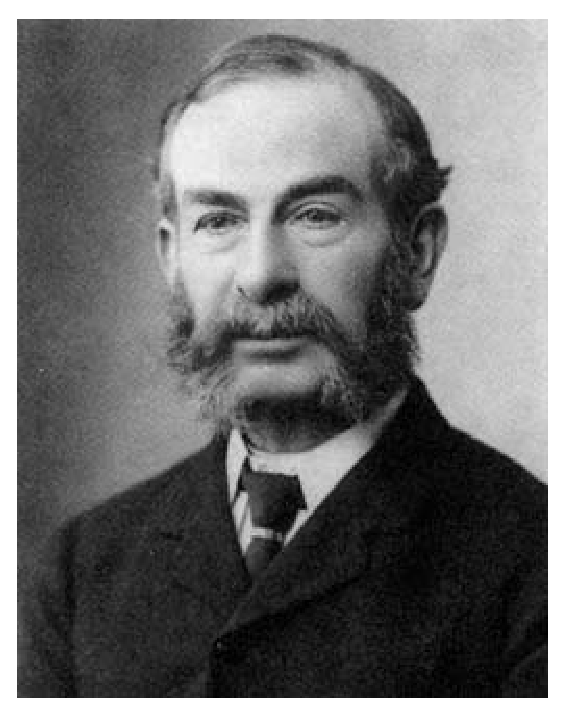
\includegraphics[width=0.9\linewidth]{EdwardRouth.eps} 
    \caption*{\index{Routh, Edward}Edward John Routh (1831-1907), 
             mathématicien anglais.}
\end{marginfigure}
%-------------------------------------------------------------------------------
pour déterminer si ce polynôme possède des racines toutes à partie réelle 
strictement négative. Les polynômes de ce type sont dits en mathématiques 
de Hurwitz\footnote{Un polynôme de Hurwitz est un polynôme à 
coefficients réels dont les racines sont toutes à partie réelle strictement 
négative.}.
C'est pourquoi le critère suivant est également connu sous le nom de 
\textbf{critère de Routh-Hurwitz}.
%-------------------------------------------------------------------------------
\begin{marginfigure}
    \centering
    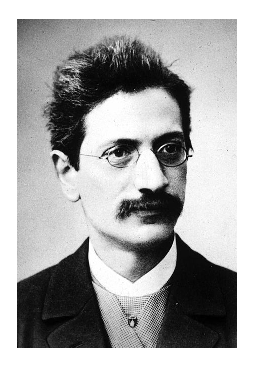
\includegraphics[width=0.9\linewidth]{AdolfHurwitz.eps} 
    \caption*{\index{Hurwitz, Adolf}Adolf Hurwitz (1859-1919),
    mathématicien allemand.}
\end{marginfigure}
%-------------------------------------------------------------------------------
Il est possible de conclure sur la nature des racines d'un polynôme 
en étudiant ses coefficients. Le critère de Routh-Hurwitz se base sur 
cette propriété en posant deux conditions pour établir qu'un polynôme est 
un polynôme de Hurwitz. Dans le cas de l'application de la stabilité des 
systèmes linéaires asservis, la première condition s'énonce 
de la façon suivante :
%-------------------------------------------------------------------------------
\begin{criteria}{Condition nécessaire de Routh-Hurwitz }
    \textbf{Un système asservi d'ordre $n$ est stable en boucle fermée 
    si tous les coefficients ($b_i\forall i\neq n$) de son équation 
    caractéristique sont de même signe que $b_n$.}
\end{criteria}
%-------------------------------------------------------------------------------
\textbf{Cette condition nécessaire s'avère suffisante si le système est du 
premier ou du second ordre.} Pour un ordre supérieur il faut construire le 
tableau de Routh à partir des coefficients de $D(p)$,
pour appliquer une condition supplémentaire. 
%%%%%%%%%%%%%%%%%%%%%%%%%%%%%%%%%%%%%%%%%%%%%%%%%%%%%%%%%%%%%%%%%%%%%%%%%%%%%%%%
%%%%%%%%%%%%%%%%%%%%%%%%%%%%%%%%%%%%%%%%%%%%%%%%%%%%%%%%%%%%%%%%%%%%%%%%%%%%%%%%
\subsection{Tableau de Routh}
%%%%%%%%%%%%%%%%%%%%%%%%%%%%%%%%%%%%%%%%%%%%%%%%%%%%%%%%%%%%%%%%%%%%%%%%%%%%%%%%
%%%%%%%%%%%%%%%%%%%%%%%%%%%%%%%%%%%%%%%%%%%%%%%%%%%%%%%%%%%%%%%%%%%%%%%%%%%%%%%%
Dans le cas où la condition nécessaire est respectée et $n>2$, il faut 
constuire le \textbf{tableau de Routh} à partir des coefficients de l'équation 
caractéristique de la fonction de transfert en boucle fermée.
\newpage
\restoregeometry
\captionsetup{width=0.9\linewidth}
Le tableau de Routh est constitué de $n$ lignes et de $k$ colonnes 
où $k=n/2+1$\footnote{On réalise ici une division entière. Par exemple 
si $n=5$, $k=2+1=3$ et si $n=6$, $k=3+1=4$}. L'élément $A_{ij}$ correspond 
à l'élément de la $i$-ème ligne et $j$-ème colonne.
\[
\begin{matrix}
    p^n    \\
    p^{n-1}\\
    p^{n-2}\\
    p^{n-3}\\
    \vdots \\
    p^1    \\
    p^0    \\
\end{matrix}
\begin{vmatrix}
  A_{11}     & A_{12}     & A_{13}     & \cdots & A_{1(k-1)}     & A_{1k}  \\
  A_{21}     & A_{22}     & A_{23}     & \cdots & A_{2(k-1)}     & A_{2k}  \\
  A_{31}     & A_{32}     & A_{33}     & \cdots & A_{3(k-1)}     & A_{3k}  \\
  A_{41}     & A_{42}     & A_{43}     & \cdots & A_{4(k-1)}     & A_{4k}  \\
  \vdots     & \vdots     & \vdots     & A_{ij} & \vdots         & \vdots  \\
  A_{(n-1)1} & A_{(n-1)2} & A_{(n-1)3} & \cdots & A_{(n-1)(k-1)} & A_{(n-1)k}\\
  A_{n1}     & A_{n2}     & A_{n3}     & \cdots & A_{n(k-1)}     & A_{nk}
\end{vmatrix}
\]

Les deux premières lignes du tableau sont directement construites à partir 
des coefficients de $D(p)$.
\[
    \textbf{paire}\qquad\quad
\begin{matrix}
    p^n    \\
    p^{n-1}\\
    \hline
    \vdots \\
\end{matrix}
\begin{vmatrix}
    b_n       & b_{n-2}    & b_{n-4}    & \cdots & b_2        & b_0  \\
    b_{n-1}   & b_{n-3}    & b_{n-5}    & \cdots & b_1        & 0    \\
    \hline
    \vdots    & \vdots     & \vdots     & \vdots & \vdots     & \vdots  \\
    \end{vmatrix}
\]
si $n$ est impaire la dernière colonne de la seconde ligne est non-nulle:
\[
    \textbf{impaire}\qquad
\begin{matrix}
    p^n    \\
    p^{n-1}\\
    \hline
    \vdots \\
\end{matrix}
\begin{vmatrix}
    b_n       & b_{n-2}    & b_{n-4}    & \cdots & b_3            & b_1    \\
    b_{n-1}   & b_{n-3}    & b_{n-5}    & \cdots & b_2            & b_0    \\
    \hline
    \vdots    & \vdots     & \vdots     & \vdots & \vdots         & \vdots \\
    \end{vmatrix}
\]

Les éléments de la troisième ligne sont construits à partir du 
déterminant\footnote{Le déterminant d'une matrice 2$\times$2 
est tel que $\begin{vmatrix} a & b \\ c & d \end{vmatrix}=ad-bc$} des 
élements des deux premières lignes.
\[
\begin{matrix}
    p^n    \\
    p^{n-1}\\
    \hline
    p^{n-2}\\
    \vdots \\
\end{matrix}
\begin{vmatrix}
    \textcolor{col4}{b_n}       & \textcolor{col4}{b_{n-2}}    & b_{n-4}    
                               & \cdots & b_3            & b_1         \\
    \textcolor{col4}{b_{n-1}}   & \textcolor{col4}{b_{n-3}}    & b_{n-5}    
                               & \cdots & b_2            & b_0         \\
    \hline
    %\hmm{A_{31}}{col4}   & A_{32}     & A_{33} & \cdots & \cdots  & \cdots \\
    A_{31}  & A_{32}     & A_{33}     & \cdots & \cdots         & \cdots   \\
    \vdots    & \vdots     & \vdots     & \vdots & \vdots         & \vdots \\
\end{vmatrix}
\Rightarrow
A_{31}=-\dfrac{1}{b_{n-1}}
\begin{vmatrix} b_{n}  & b_{n-2} \\ b_{n-1} & b_{n-3}
\end{vmatrix}
\]

\[
\begin{matrix}
    p^n    \\
    p^{n-1}\\
    \hline
    p^{n-2}\\
    \vdots \\
\end{matrix}
\begin{vmatrix}
    \textcolor{col1}{b_n}       & b_{n-2}    & \textcolor{col1}{b_{n-4}}    
    & \cdots & b_3        & b_1         \\
    \textcolor{col1}{b_{n-1}}   & b_{n-3}    & \textcolor{col1}{b_{n-5}}    
    & \cdots & b_2            & b_0         \\
    \hline
    %A_{31}    & \hmm{A_{32}}{col1}     & A_{33} & \cdots & \cdots& \cdots  \\
    A_{31}    & A_{32}     & A_{33}     & \cdots & \cdots         & \cdots  \\
    \vdots    & \vdots     & \vdots     & \vdots & \vdots         & \vdots  \\
\end{vmatrix}
\Rightarrow
A_{32}=-\dfrac{1}{b_{n-1}}\begin{vmatrix} b_{n}  & b_{n-4} \\ b_{n-1} & b_{n-5}
\end{vmatrix}
\]

On construit de la même manière la quatrième ligne :
\[
\begin{matrix}
    p^n    \\
    p^{n-1}\\
    \hline
    p^{n-2}\\
    p^{n-3}\\
    \vdots \\
\end{matrix}
\begin{vmatrix}
    b_n       & b_{n-2}    & b_{n-4}    & \cdots & b_3            & b_1 \\
     \textcolor{col4}{b_{n-1}}   & \textcolor{col4}{b_{n-3}}    & b_{n-5}    
                                & \cdots & b_2            & b_0         \\
    \hline
     \textcolor{col4}{A_{31}}    &  \textcolor{col4}{A_{32}}    & A_{33}    
                                & \cdots & \cdots         & \cdots      \\
    A_{41}   & A_{42}     & A_{43}    & \cdots & \cdots   & \cdots      \\
    \vdots   & \vdots     & \vdots    & \vdots & \vdots   & \vdots      \\
    \end{vmatrix}
\Rightarrow
A_{41}=-\dfrac{1}{A_{31}}
\begin{vmatrix} 
A_{21} & A_{22} \\ A_{31} & A_{22}
\end{vmatrix}
\]

\[
\begin{matrix}
    p^n    \\
    p^{n-1}\\
    \hline
    p^{n-2}\\
    p^{n-3}\\
    \vdots \\
\end{matrix}
\begin{vmatrix}
    b_n       & b_{n-2}    & b_{n-4}    & \cdots & b_3            & b_1  \\
    \textcolor{col1}{b_{n-1}}   &  b_{n-3}    & \textcolor{col1}{b_{n-5}}    
    & \cdots & b_2            & b_0         \\
    \hline
    \textcolor{col1}{A_{31}}     &  A_{32}    & \textcolor{col1}{A_{33}}    
    & \cdots & \cdots         & \cdots      \\
    A_{41}      & A_{42}     & A_{43}    & \cdots & \cdots    & \cdots   \\
    \vdots    & \vdots     & \vdots     & \vdots & \vdots     & \vdots   \\
    \end{vmatrix}
    \Rightarrow
    A_{42}=-\dfrac{1}{A_{31}}
    \begin{vmatrix} 
        A_{21} & A_{23} \\ A_{31} & A_{33} 
\end{vmatrix}
\]
Et ainsi de suite jusque la dernière ligne du tableau. 
La formule générale pour obtenir l'élément $A_{ij}$ est alors :
%-------------------------------------------------------------------------------
\begin{bequation}[ams align]
    A_{ij}=-\dfrac{1}{A_{(i-1)1}}
    \begin{vmatrix} 
        A_{(i-2)1} & A_{(i-2)(j+1)} \\ 
        A_{(i-1)1} & A_{(i-1)(j+1)} 
    \end{vmatrix}
\end{bequation}
%-------------------------------------------------------------------------------
Le critère s'applique sur la première colonne ainsi construit dite 
\textbf{colonne des pivots} du tableau de Routh. 
\[
\begin{matrix}
    p^n    \\
    p^{n-1}\\
    p^{n-2}\\
    p^{n-3}\\
    \vdots \\
    p^1    \\
    p^0    \\
\end{matrix}
\begin{vmatrix}
    b_n\DoTikzmark{-1ex}{1.75ex}{n1} & b_{n-2} & b_{n-4}& \cdots & b_2  & b_0\\
    b_{n-1}              & b_{n-3}   & b_{n-5} & \cdots & b_1      & 0 \\
    A_{31}               & A_{32}    & A_{33}  & \cdots & A_{3(k-1)} & 0 \\
    A_{41}               & A_{42}    & A_{43}  & \cdots & 0        & 0 \\
    \vdots               & \vdots    & \vdots  & \vdots & \vdots   & 0 \\
    A_{(n-1)1}           & A_{(n-1)2}& 0       & \cdots & 0        & 0 \\
    b_0\DoTikzmark{-1ex}{-0ex}{n2}    & 0       & 0      & \cdots & 0 & 0
\end{vmatrix}
\]
\colrow[col3,opacity=.2]{n1}{n2}
%-------------------------------------------------------------------------------
\begin{criteria}{Critère de Routh-Hurtwitz}
    \textbf{Un système asservi est stable en boucle fermée
            si tous les termes de la colonne des pivots 
            du tableau de Routh du polynôme caractéristique 
            de la fonction de transfert en boucle fermée sont de même signes.}
\end{criteria}
%-------------------------------------------------------------------------------
%%%%%%%%%%%%%%%%%%%%%%%%%%%%%%%%%%%%%%%%%%%%%%%%%%%%%%%%%%%%%%%%%%%%%%%%%%%%%%%%
\paragraph{Remarques:}
%%%%%%%%%%%%%%%%%%%%%%%%%%%%%%%%%%%%%%%%%%%%%%%%%%%%%%%%%%%%%%%%%%%%%%%%%%%%%%%%
Le nombre de changement de signe, nous donne le nombre de pôles à partie 
réelle positives (instables) de la fonction de transfert en boucle fermée.
%%%%%%%%%%%%%%%%%%%%%%%%%%%%%%%%%%%%%%%%%%%%%%%%%%%%%%%%%%%%%%%%%%%%%%%%%%%%%%%%
\paragraph{Propriétés du tableau de Routh}
%%%%%%%%%%%%%%%%%%%%%%%%%%%%%%%%%%%%%%%%%%%%%%%%%%%%%%%%%%%%%%%%%%%%%%%%%%%%%%%%
Nous énonçons ici quelques propriétés du tableau de Routh 
pour faciliter ou permettre l'application du critère dans 
des cas particuliers~\cite{Ostertag}. 
%-------------------------------------------------------------------------------
\begin{itemize}
    \item Pour simplifier les calculs, il est possible de factorisée par un 
          entier une ligne du tableau.
    \item Dans le cas où le tableau présente un zéro dans la première 
          colonne, il est possible de remplacer par une variable $\epsilon$, 
          et de prendre la limite lorsque $\epsilon\rightarrow 0^+$ ou 
          $\epsilon\rightarrow 0^-$ selon le signe de la colonne des pivots
          qui respecterait le critère.
    \item Une ligne de zéros pour les coefficients de l'avant-dernière ligne 
          du tableau de Routh indique que le polynôme du dénominateur de la 
          fonction de transfert possède une paire de pôles, qui sont racines de 
          l'équation auxiliaire :
    \[
        Ap^2+B=0
    \]
    où $A$ et $B$ sont les coefficients de la ligne précédente du tableau. 
    On peut alors continuer le tableau en remplaçant la ligne de coefficients 
    nuls par les coefficients de la dérivée de l'équation auxiliaire. 
    
    Une ligne de zéro implique la présence d'une paire de racines imaginaires 
    pures donnant lieu à une forme sinuso\"idale dans la réponse transitoire.
    Le système diverge en oscillant s'il y a au moins une racine à partie 
    réelle positive, ou il converge vers des oscillations entretenues si les 
    autres racines ont toutes une partie réelle négative.
\end{itemize}
%-------------------------------------------------------------------------------
%%%%%%%%%%%%%%%%%%%%%%%%%%%%%%%%%%%%%%%%%%%%%%%%%%%%%%%%%%%%%%%%%%%%%%%%%%%%%%%%
%%%%%%%%%%%%%%%%%%%%%%%%%%%%%%%%%%%%%%%%%%%%%%%%%%%%%%%%%%%%%%%%%%%%%%%%%%%%%%%%
\subsection{Exemple d'application du critère de Routh-Hurwitz}
%%%%%%%%%%%%%%%%%%%%%%%%%%%%%%%%%%%%%%%%%%%%%%%%%%%%%%%%%%%%%%%%%%%%%%%%%%%%%%%%
%%%%%%%%%%%%%%%%%%%%%%%%%%%%%%%%%%%%%%%%%%%%%%%%%%%%%%%%%%%%%%%%%%%%%%%%%%%%%%%%

La particularité du critère de Routh-Hurwitz est de permettre d'étudier les 
conditions de stabilité d'un système en fonction des paramètres de la fonction 
de transfert en boucle ouverte.

Dans l'exemple ci-dessous, nous allons considérer un système asservi 
caractérisé par fonction de transfert en boucle ouverte défini par un gain $K$
dont l'on souhaite déterminer la valeur pour assurer la stabilité du système en 
boucle fermée.

Soit un système asservi défini par le schéma-bloc suivant :
%-------------------------------------------------------------------------------
\begin{center}
    \tikzsetnextfilename{routh_exemple-chap_stab-ext}
    \input{tikz/routh_exemple-chap_stab.tex}
\end{center}
%-------------------------------------------------------------------------------
La fonction de transfert en boucle fermée $H_{BF}(p)$ s'écrit :
\[
    H_{BF}(p)=\dfrac{H_{BO}(p)}{1+H_{BO}(p)}=\dfrac{K}{p^3+p^2+3p+K}.
\]
L'équation caractéristique $D(p)$ de $H_{BF}$ est donc 
\[
    D(p)=p^3+p^2+3p+K,
\]
Nous constatons que le système est d'ordre 3 de coefficients :
%-------------------------------------------------------------------------------
\begin{align*}
    b_3&=1\\
    b_2&=1\\
    b_1&=3\\
    b_0&=K
\end{align*}
%-------------------------------------------------------------------------------
Le critère nécessaire de Routh est donc respecté pour $K>0$. L'équation 
caractéristique étant d'ordre 3, il nous faut construire le tableau de Routh, 
afin de vérifier le critère supplémentaire :
\[
\begin{matrix}
    p^3 \\
    p^2 \\
    \hline
    p^1 \\
    p^0 \\
\end{matrix}
\begin{vmatrix}
     1      & 3  \\
     1      & K  \\
    \hline
    A_{31}  & 0  \\
    A_{41}  & 0    
\end{vmatrix}
\]

\[
A_{31}=-\begin{vmatrix}1 & 3 \\ 1 & K\end{vmatrix}=3-K
\]

\[
A_{41}=-\dfrac{1}{A_{31}}\begin{vmatrix} 1 & K \\ A_{31} & 0 \end{vmatrix}=K
\]
\[
\begin{matrix}
    p^3 \\
    p^2 \\
    p^1 \\
    p^0 \\
\end{matrix}
\begin{vmatrix}
    1\DoTikzmark{-0.6ex}{1.75ex}{n3}   & 3  \\
    1\DoTikzmark{-0.6ex}{-6ex}{n4}     & K  \\
    3-K                      & 0  \\
    K                        & 0    
    \end{vmatrix}
\]
\colrow[col3,opacity=.2]{n3}{n4}

La colonne des pivots sont tous de même signe si $3-K>0$ et $K>0$ (déjà établie 
par la condition nécessaire de Routh). La condition sur $K$ pour que le 
système soit stable en boucle fermée est donc :
\[
    0<K<3
\]
%%%%%%%%%%%%%%%%%%%%%%%%%%%%%%%%%%%%%%%%%%%%%%%%%%%%%%%%%%%%%%%%%%%%%%%%%%%%%%%%
%%%%%%%%%%%%%%%%%%%%%%%%%%%%%%%%%%%%%%%%%%%%%%%%%%%%%%%%%%%%%%%%%%%%%%%%%%%%%%%%
%%%%%%%%%%%%%%%%%%%%%%%%%%%%%%%%%%%%%%%%%%%%%%%%%%%%%%%%%%%%%%%%%%%%%%%%%%%%%%%%
\section{Critère graphique du revers
\index{Critère de stabilité! du revers}}
%%%%%%%%%%%%%%%%%%%%%%%%%%%%%%%%%%%%%%%%%%%%%%%%%%%%%%%%%%%%%%%%%%%%%%%%%%%%%%%%
%%%%%%%%%%%%%%%%%%%%%%%%%%%%%%%%%%%%%%%%%%%%%%%%%%%%%%%%%%%%%%%%%%%%%%%%%%%%%%%%
%%%%%%%%%%%%%%%%%%%%%%%%%%%%%%%%%%%%%%%%%%%%%%%%%%%%%%%%%%%%%%%%%%%%%%%%%%%%%%%%
Le critère de Routh s'applique sur la fonction de transfert en boucle fermée. 
Les critères graphiques que nous allons maintenant établir 
permettent d'étudier la stabilité du système en boucle fermée en considérant 
le système en boucle ouverte.

Pour celà considèrons la boucle de contre réaction unitaire 
pour l'asservissement d'un système de fonction de transfert $H(p)$, telle que :
%-------------------------------------------------------------------------------
\begin{center}
    \tikzsetnextfilename{sb_revers-chap_stab-ext}
    \input{tikz/sb_revers-chap_stab.tex}
\end{center}
%-------------------------------------------------------------------------------
la fonction de transfert en boucle ouverte $H_{BO}(p)$ est simplement donné 
par $H(p)$, et comme nous l'avons déjà rencontré à plusieurs occasions, la 
fonction de transfert en boucle fermée $H_{BF}(p)$ est égale à 
\[
    H_{BF}(p)=\dfrac{N(p)}{D(p)}=\dfrac{H_{BO}(p)}{1+H_{BO}(p)},
\]
\'Etudier les pôles de l'équation caractéristique $D(p)=0$ est équivalent 
à étudier l'équation $1+H_{BO}(p)=0$, ou encore 
\[
    D(p)=0\Leftrightarrow1+H_{BO}(p)=0\Leftrightarrow H_{BO}(p)=-1
\]
Il est alors possible d'étudier la fonction de transfert en boucle ouverte par 
rapport à -1 plutôt que par rapport à l'origine. 
%Ce \textbf{point critique}\index{Point critique} du 
%plan complexe $(-1,0)$ de $H_{BO}(p)$.

Pour montrer quelques propriétés de $1+H_{BO}(p)$, nous allons réecrire
ces fonctions de transferts en fonction des polynomes du numérateur et
du dénominateur de la boucle ouverte.
En effet, la fonction de transfert en boucle ouverte
est en générale une fraction rationnelle de la forme:
%-------------------------------------------------------------------------------
\begin{align*}
H_{BO}(p)=\dfrac{N_{BO}(p)}{D_{BO}(p)} \\
1+H_{BO}(p)=\dfrac{N_{BO}(p)+D_{BO}(p)}{D_{BO}(p)}
\end{align*}
%-------------------------------------------------------------------------------
on a alors pour la fonction de transfert en boucle fermée, 
\[
H_{BF}(p)=\dfrac{\dfrac{N_{BO}(p)}{D_{BO}(p)}}{1+\dfrac{N_{BO}(p)}{D_{BO}(p)}}
         =\dfrac{N_{BO}(p)}{D_{BO}(p)+N_{BO}(p)}
\]
Nous remarquons alors que les zéros de $1+H_{BO}(p)$ 
sont les pôles de la fonction de transfert en boucle fermée 
$H_{BF}(p)$ et que les pôles de $1+H_{BO}(p)$ co\"incident avec 
les pôles de $H_{BO}(p)$. Il est donc possible de 
réinterpréter la condition stabilité d'un système asservi :
%-------------------------------------------------------------------------------
\begin{criteria}{Condition de stabilité d'un système asservi (2)}
    \textbf{Un système asservi est stable en boucle fermée si sa fonction 
    de transfert en boucle ouverte ne possède aucun \emph{zéros} à partie 
    réelle positive.}
\end{criteria}
%-------------------------------------------------------------------------------
Nous allons établir un critère que nous pourrons appliquer sur la réponse 
harmonique et ses différentes représentations graphiques.

Supposons le système asservi précédent décrit par la fonction de transfert 
en boucle ouverte $H_{BO}(p)$. Par définition cette fonction de transfert 
est le rapport de la sortie $S(p)$ sur l'écart $\epsilon(p)$ que l'on 
souhaite minimiser.
\[
    S(p)=H_{BO}(p)\epsilon(p)
\]
Considérons une entrée $e(t)$ sinuso\"idale de la forme :
\[
    e(t)=E_0\sin{\omega t}
\]
au premier instant, on a alors 
\[
    \epsilon(t)=E_0\sin{\omega t}
\]
en régime permanent la sortie est alors de la forme (c.f~\cref{chap-repfreq}) :
\[
    s(t)=E_0|H_{BO}(\jw)|\sin{(\omega t+\phi)}
\]
l'écart $\epsilon(t)=e(t)-s(t)$ est maximum pour une sortie en opposition 
de phase. Il existe donc une pulsation $\omega_\pi$ pour laquelle:
%-------------------------------------------------------------------------------
\begin{align*}
    \phi=\arg{H_{BO}(j\omega_\pi)}=-\pi
\end{align*}
%-------------------------------------------------------------------------------
En Pour cette pulsation et ce déphasage: 
\[
    S(p)=-\big|H_{BO}(j\omega_\pi)\big|\epsilon(p)
\]
en posant $K=|H_{BO}(j\omega_\pi)|$, on identifie la \gls{ftbo} a :
\[
    H_{BO}(p)=-K
\]
L'écart dans le domaine de Laplace devient:
%-------------------------------------------------------------------------------
\begin{align*}
    \epsilon(p)&=E(p)-S(p)\\
    \epsilon(p)&=E(p)+K\epsilon(p)
\end{align*}
%-------------------------------------------------------------------------------
Remplaçons à nouveau $\epsilon(p)$ par sa définition (pour simuler une 
deuxième boucle) : 
%-------------------------------------------------------------------------------
\begin{align*}
    \epsilon(p)&=E(p)+K(E(p)-S(p))=E(p)(1+K)+K^2\epsilon(p)
\end{align*}
%-------------------------------------------------------------------------------
et ainsi de suite :
%-------------------------------------------------------------------------------
\begin{align*}
    \epsilon(p)&=E(p)(1+K)+K^2\left(E(p)-S(p)\right)
                =E(p)(1+K+K^2)+K^3\epsilon(p)\\
\end{align*}
%-------------------------------------------------------------------------------
on obtient après $n$ substitutions :
\[
\epsilon(p)=E(p)\sum_{i=0}^{n}K^i+K^n\epsilon(p)
\]
La stabilité du système est alors liée à la convergence de cette somme.
La somme diverge si $K\geq1$ et converge si $K<1$. 
\textbf{Autrement dit le système est stable en boucle fermée 
pour $\big|H_{BO}(\jw)\big|<1$.}

Nous pouvons donc énoncer le critère de stabilité dit du revers :
%-------------------------------------------------------------------------------
\begin{criteria}{Critère de stabilité du revers}
    \textbf{Un système est stable en boucle fermée si lorque le 
    déphasage en boucle ouverte est de -180\degree~le module $|H_{BO}(\jw)|$ 
    est strictement inférieur à 1.}
    Formellement, pour une pulsation $\omega_{\pi}$ telle que 
    $\phi=\arg{\left(H_{BO}(j\omega_\pi)\right)}=-\pi$, 
    le système est stable en boucle fermée si $|H_{BO}(j\omega_\pi)|<1$ ou 
    $20\log{|H_{BO}(j\omega_\pi)|}<\SI{0}{\dB}$.
\end{criteria}
%-------------------------------------------------------------------------------
Dans le plan complexe, un  déphasage de -$\pi$ et un gain naturel de 1 
correspond au point de coordonnées $(-1,0)$ ce que nous avons défini comme 
le point critique à partir de l'équation caractéristique $1+H_{BO}=0$. 
Ce critère revient donc à étudier graphiquement le comportement 
de la réponse harmonique de $H_{BO}(\jw)$ par rapport au point critique.

Nous avons vu que la réponse harmonique peut avoir plusieurs représentations
graphiques (c.f~\Cref{chap-repfreq}). Nous allons maintenant appliquer le 
critère à ces différentes représentations graphiques.

\clearpage
%%%%%%%%%%%%%%%%%%%%%%%%%%%%%%%%%%%%%%%%%%%%%%%%%%%%%%%%%%%%%%%%%%%%%%%%%%%%%%%%
%%%%%%%%%%%%%%%%%%%%%%%%%%%%%%%%%%%%%%%%%%%%%%%%%%%%%%%%%%%%%%%%%%%%%%%%%%%%%%%%
\subsection{Critère du revers dans le plan de Nyquist
\index{Critère de stabilité! du revers! dans le plan de Nyquist}}
%%%%%%%%%%%%%%%%%%%%%%%%%%%%%%%%%%%%%%%%%%%%%%%%%%%%%%%%%%%%%%%%%%%%%%%%%%%%%%%%
%%%%%%%%%%%%%%%%%%%%%%%%%%%%%%%%%%%%%%%%%%%%%%%%%%%%%%%%%%%%%%%%%%%%%%%%%%%%%%%%

Pour énoncer le critère du revers dans le plan de Nyquist. Il nous faut tracer
le lieu de Nyquist de la fonction de transfert en boucle ouverte et observer 
comment il se comporte par rapport au point critique de coordonnées (-1,0) 
dans le plan complexe de $H_{BO}(\jw)$. La~\cref{fig-nyquist_revers} présente 
les lieux de Nyquist de trois systèmes: stable, instable et critique. Observons
que dans le cas stable, le lieu de déphasage $\phi=-\pi$ (c.a.d lorsque le lieu
coupe l'axe des réels négatifs), le module ou le gain naturel $G(\omega)$ (ou 
encore la distance à l'origine) est inférieur à 1. Dans le cas instable ce gain 
est supérieur à 1. Nous appelerons critique le système dont le lieu de Nyquist 
passe par le point critique de coordonnées (-1,0).
%-------------------------------------------------------------------------------
\begin{figure}[!h]
    \centering
    \tikzsetnextfilename{critere_revers_nyquist-chap_stab-ext}
    \input{tikz/critere_revers_nyquist-chap_stab.tex}
    \caption{Représentation schématique de lieux de Nyquist de la fonction 
             de transfert en boucle ouverte de trois systèmes asservis: 
             stable, critique et instable. \label{fig-nyquist_revers}}
\end{figure}
%-------------------------------------------------------------------------------
Nous pouvons maintenant formuler le critère du revers de Nyquist :
%-------------------------------------------------------------------------------
\begin{criteria}{Critère du revers de Nyquist}
\textbf{Un système est stable en boucle fermée si lorsque parcourant 
        le lieu de Nyquist de la boucle ouverte dans le sens des 
        pulsations croissantes, on laisse le point critique sur la 
        \emph{gauche}.}
\end{criteria}
%-------------------------------------------------------------------------------
%\newpage
%%%%%%%%%%%%%%%%%%%%%%%%%%%%%%%%%%%%%%%%%%%%%%%%%%%%%%%%%%%%%%%%%%%%%%%%%%%%%%%%
%%%%%%%%%%%%%%%%%%%%%%%%%%%%%%%%%%%%%%%%%%%%%%%%%%%%%%%%%%%%%%%%%%%%%%%%%%%%%%%%
\subsection{Critère du revers dans le plan de Black
\index{Critère de stabilité! du revers! dans le plan de Black}}
%%%%%%%%%%%%%%%%%%%%%%%%%%%%%%%%%%%%%%%%%%%%%%%%%%%%%%%%%%%%%%%%%%%%%%%%%%%%%%%%
%%%%%%%%%%%%%%%%%%%%%%%%%%%%%%%%%%%%%%%%%%%%%%%%%%%%%%%%%%%%%%%%%%%%%%%%%%%%%%%%
\acpl
%-------------------------------------------------------------------------------
\begin{figure}[!h]
    \centering
    \tikzsetnextfilename{critere_revers_black-chap_stab-ext}
    \begin{tikzpicture}
    \begin{axis}
    [
        height=8cm,
        width=8cm,
        axis lines = center,
        axis line style = thick,
        ticks=none,
        enlargelimits=false,
        xlabel=$\phi$,
        ylabel=$G_{dB}$,
        xlabel style={below right},
        ylabel style={left},
        ymin=-150,
        ymax=60,
        xmin=-270,
        xmax=70
    ]
    \def\da{0.6}
    \def\db{5.0}
    \def\dk{4}
    \def\dpp{1.35}
    \def\colru{col4}
    \addplot[\colru,thick,domain=1e-2:1e-1,samples=100]
    ({-\dpp*atan2(\da*x,(1-\db*x*x))},
     {-\dk*10*log10((1-\db*x*x)*(1-\db*x*x)+\da*\da*x*x)}); 
    \addplot[\colru,thick,domain=1e-1:1e0,samples=100,-{Latex[length=2mm]}] 
    ({-\dpp*atan2(\da*x,(1-\db*x*x))},
     {-\dk*10*log10((1-\db*x*x)*(1-\db*x*x)+\da*\da*x*x)}); 
    \addplot[\colru,thick,domain=0.9e0:1e1,samples=100]  
    ({-\dpp*atan2(\da*x,(1-\db*x*x))},
     {-\dk*10*log10((1-\db*x*x)*(1-\db*x*x)+\da*\da*x*x)});
    \addplot[\colru,thick,domain=1e1:1e2,samples=100]  
    ({-\dpp*atan2(\da*x,(1-\db*x*x))},
     {-\dk*10*log10((1-\db*x*x)*(1-\db*x*x)+\da*\da*x*x)});
    \node [\colru,right]  at (axis cs:  -260, 40.0) {\textbf{instable}};

    \def\da{0.6}
    \def\db{1.0}
    \def\dk{1.5}
    \def\dpp{0.95}
    \edef\colrd{col3}
    \addplot[\colrd,thick,domain=1e-2:1e-1,samples=100]
    ({-\dpp*atan2(\da*x,(1-\db*x*x))},
     {-\dk*10*log10((1-\db*x*x)*(1-\db*x*x)+\da*\da*x*x)}); 
    \addplot[\colrd,thick,domain=1e-1:1e0,samples=100] 
    ({-\dpp*atan2(\da*x,(1-\db*x*x))},
     {-\dk*10*log10((1-\db*x*x)*(1-\db*x*x)+\da*\da*x*x)}); 
    \addplot[\colrd,thick,domain=1e0:1e1,samples=100,-{Latex[length=2mm]}] 
    ({-\dpp*atan2(\da*x,(1-\db*x*x))},
     {-\dk*10*log10((1-\db*x*x)*(1-\db*x*x)+\da*\da*x*x)});
    \addplot[\colrd,thick,domain=0.9e1:1e2,samples=100] 
    ({-\dpp*atan2(\da*x,(1-\db*x*x))},
     {-\dk*10*log10((1-\db*x*x)*(1-\db*x*x)+\da*\da*x*x)});
    \node [\colrd,right]  at (axis cs:  -140, -60.0)   {\textbf{stable}};

    \def\da{0.6}
    \def\db{4.0}
    \def\dk{1.75}
    \def\dpp{1.15}
    \edef\colrt{col1}
    \addplot[\colrt,thick,domain=1e-2:1e-1,samples=100]
    ({-\dpp*atan2(\da*x,(1-\db*x*x))},
     {-\dk*10*log10((1-\db*x*x)*(1-\db*x*x)+\da*\da*x*x)}); 
    \addplot[\colrt,thick,domain=1e-1:1e0,samples=100] 
    ({-\dpp*atan2(\da*x,(1-\db*x*x))},
     {-\dk*10*log10((1-\db*x*x)*(1-\db*x*x)+\da*\da*x*x)}); 
    \addplot[\colrt,thick,domain=1e0:1e1,samples=100,-{Latex[length=2mm]}] 
    ({-\dpp*atan2(\da*x,(1-\db*x*x))},
     {-\dk*10*log10((1-\db*x*x)*(1-\db*x*x)+\da*\da*x*x)});
    \addplot[\colrt,thick,domain=0.9e1:1e2,samples=100] 
    ({-\dpp*atan2(\da*x,(1-\db*x*x))},
     {-\dk*10*log10((1-\db*x*x)*(1-\db*x*x)+\da*\da*x*x)});
    \draw[draw=none,fill=black] (axis cs:-180,0) circle (2pt) node[above] 
    {$(-180,0\mathrm{dB})$};
    \node [\colrt,right]  at (axis cs:  -200, -140.0) {\textbf{critique}};
\end{axis}
\end{tikzpicture}

    \caption{Représentation schématique de lieux de Black de la 
             fonction de transfert en boucle ouverte de trois systèmes 
             asservis: stable, critique et instable.
             \label{fig-black_revers}}
\end{figure}
%-------------------------------------------------------------------------------
%-------------------------------------------------------------------------------
\begin{criteria}{Critère du revers de Black}
\textbf{Un système est stable en boucle fermée si lorsque parcourant 
        le lieu de Black de la boucle ouverte dans le sens des 
        pulsations croissantes, on laisse le point critique sur 
        la \emph{droite}.}
\end{criteria}
%-------------------------------------------------------------------------------
%\newpage
%%%%%%%%%%%%%%%%%%%%%%%%%%%%%%%%%%%%%%%%%%%%%%%%%%%%%%%%%%%%%%%%%%%%%%%%%%%%%%%%
%%%%%%%%%%%%%%%%%%%%%%%%%%%%%%%%%%%%%%%%%%%%%%%%%%%%%%%%%%%%%%%%%%%%%%%%%%%%%%%%
\subsection{Critère du revers dans le plan de Bode
\index{Critère de stabilité! du revers! dans le plan de Bode}}
%%%%%%%%%%%%%%%%%%%%%%%%%%%%%%%%%%%%%%%%%%%%%%%%%%%%%%%%%%%%%%%%%%%%%%%%%%%%%%%%
%%%%%%%%%%%%%%%%%%%%%%%%%%%%%%%%%%%%%%%%%%%%%%%%%%%%%%%%%%%%%%%%%%%%%%%%%%%%%%%%
Il est possible d'appliquer le critère du revers au lieu de transfert de Bode
en boucle ouverte. Le point critique
dans le plan de Bode est représenté par deux verticales coupant les deux 
graphes en gain et en déphasage. De ce fait il faut vérifier deux conditions 
pour respecter le critère du revers dans le plan de Bode 
%-------------------------------------------------------------------------------
\begin{criteria}{Critère du revers de Bode (1)}
\textbf{Un système est stable en boucle fermée si, pour la pulsation 
        $\omega_{1}$ telle que le module de la fonction de transfert en boucle 
        ouverte est égal à 1 (c.a.d $H_{BO}(\omega_{1})=1$ ou $\SI{0}{\dB}$), 
        le déphasage $\phi(\omega_1)$ est supérieur à -180\degree}
\end{criteria}
%-------------------------------------------------------------------------------
%-------------------------------------------------------------------------------
\begin{criteria}{Critère du revers de Bode (2)}
    \textbf{Un système est stable en boucle fermée si, pour la pulsation 
    $\omega_{c}$ (pulsation critique) telle que l'argument de la fonction de 
    transfert en boucle ouverte (déphasage) est égale à -180\degree 
    (c.a.d $\phi(\omega_c)=-180\degree$), le gain $G_{dB}(\omega_c)$ est 
    négatif.}
\end{criteria}
%-------------------------------------------------------------------------------
%-------------------------------------------------------------------------------
\begin{figure}[!h]
\centering
    \tikzsetnextfilename{critere_revers_bode-chap_stab-ext}
    \begin{tikzpicture}
    \begin{axis}
    [
        name=axx,
        ticks=none,
        axis line style = thick,
        xmode=log,
        enlargelimits=false,
        height=4.5cm,
        width=9cm,
        axis x line=center,
        axis y line=left,
        xmin=1e-2,
        xmax=1e2,
        ymin=-60,
        ymax=80,
        xlabel={$\log\omega$},
        xlabel style={below right},
        ylabel={$G_{dB}(\omega)$},
        ylabel style={left,rotate=-90,yshift=3.25em},
        clip=false,
    ]
    \def\dk{9}
    \addplot[signalr,domain=1e-2:1e2]  {\dk+50-20*log10(1+10*x*x)};
    \addplot[signalb,domain=1e-2:1e2]  {\dk+30-20*log10(1+10*x*x)};
    \addplot[signalg,domain=1e-2:1e2]  {\dk+10-20*log10(1+10*x*x)};
    \addplot [col3, mark = *]  coordinates {(3,{\dk+10-20*log10(91)})} {};
    \addplot [col1, mark = *]  coordinates {(3,{\dk+30-20*log10(91)})} {};
    \addplot [col4, mark = *]  coordinates {(3,{\dk+50-20*log10(91)})} {};
    \draw[col3,dashed]  (1e-2,{\dk+10-20*log10(91)}) 
    node[left] {$G(\omega_\pi)$} -- (3,{\dk+10-20*log10(91)});
    \draw[col4,dashed] (1e-2,{\dk+50-20*log10(91)}) 
    node[left] {$G(\omega_\pi)$} -- (3,{\dk+50-20*log10(91)}) ;
    \node (pt1) at (axis cs:3,80) {};
    \draw[]  (1e-2,0)  node[left] {\SI{0}{\dB}} -- (1e2,0);
    \node [col3,right]  at (axis cs: 1e2, -80.0) {\textbf{stable}};
    \node [col1,right]  at (axis cs: 1e2, -60.0) {\textbf{critique}};
    \node [col4,right]  at (axis cs: 1e2, -40.0) {\textbf{instable}};
    \end{axis}
    \begin{axis}
    [
        at={(axx.below south west)},yshift=-0.2cm,anchor=north west,
        ticks=none,
        axis line style = thick,
        xmode=log,
        enlargelimits=false,
        height=4.5cm,
        width=9cm,
        axis x line=center,
        axis y line=left,
        xmin=1e-2,
        xmax=1e2,
        ymin=-270,
        ymax=40,
        xlabel={$\log\omega$},
        xlabel style={below right},
        ylabel={$\hphantom{_DB}\phi(\omega)$},
        ylabel style={left,rotate=-90,yshift=3.25em},
        clip=false,
    ]
    \addplot[very thick,col5,domain=1e-2:1e2, samples=101] {-2.5*atan2(x,1)};
    \def\ttt{0.865}
    \def\ddd{9.1}
    \addplot [col3, mark = *]  coordinates {(\ttt,{-2.5*atan2(\ttt,1)})} {};
    \addplot [col1, mark = *]  coordinates {(3,{-2.5*atan2(3,1)})} {};
    \addplot [col4, mark = *]  coordinates {(\ddd,{-2.5*atan2(\ddd,1)})} {};
    \draw[col3,dashed] (1e-2,{-2.5*atan2(\ttt,1)}) 
    node[left] {$\phi(\omega_{c0})$} -- (\ttt,{-2.5*atan2(\ttt,1)}) ;
    \draw[col4,dashed]  (1e-2,{-2.5*atan2(\ddd,1)}) 
    node[left] {$\phi(\omega_{c0})$} -- (\ddd,{-2.5*atan2(\ddd,1)}) ;
    \draw[black,dashed] (1e-2,-180) node[left] {-180$\degree$} -- (1e2,-180) ;
    \end{axis}
    \draw[col3,dashed] ($(pt1)+(-1,0)$) node[above]{$\omega_{c0}$}--+(0,-7.5cm);
    \draw[col1,dashed] ($(pt1)+(0,0)$)  node[above,text width=1cm,align=center] 
    {$\omega_{c0}$} -- + (0,-7.5cm) ;
    \draw[col4,dashed] ($(pt1)+(0.9,0)$)node[above]{$\omega_{c0}$}--+(0,-7.5cm);
\end{tikzpicture}

    \caption{Représentation schématique de lieux de Bode de la fonction 
             de transfert en boucle ouverte de trois systèmes asservis: 
             stable, critique et instable.}
\end{figure}
%-------------------------------------------------------------------------------
%%%%%%%%%%%%%%%%%%%%%%%%%%%%%%%%%%%%%%%%%%%%%%%%%%%%%%%%%%%%%%%%%%%%%%%%%%%%%%%%
%%%%%%%%%%%%%%%%%%%%%%%%%%%%%%%%%%%%%%%%%%%%%%%%%%%%%%%%%%%%%%%%%%%%%%%%%%%%%%%%
%%%%%%%%%%%%%%%%%%%%%%%%%%%%%%%%%%%%%%%%%%%%%%%%%%%%%%%%%%%%%%%%%%%%%%%%%%%%%%%%
\section{Marge de stabilité et robustesse de la stabilité}
%%%%%%%%%%%%%%%%%%%%%%%%%%%%%%%%%%%%%%%%%%%%%%%%%%%%%%%%%%%%%%%%%%%%%%%%%%%%%%%%
%%%%%%%%%%%%%%%%%%%%%%%%%%%%%%%%%%%%%%%%%%%%%%%%%%%%%%%%%%%%%%%%%%%%%%%%%%%%%%%%
%%%%%%%%%%%%%%%%%%%%%%%%%%%%%%%%%%%%%%%%%%%%%%%%%%%%%%%%%%%%%%%%%%%%%%%%%%%%%%%%
Les critères de stabilité graphiques permettent de s'assurer qu'un système 
est stable ou instable (ou à la limite de la stabilité) en étudiant la réponse
harmonique. Pour estimer la proximité de la réponse harmonique au point 
critique, nous définissons les marges de stabilité. 
%%%%%%%%%%%%%%%%%%%%%%%%%%%%%%%%%%%%%%%%%%%%%%%%%%%%%%%%%%%%%%%%%%%%%%%%%%%%%%%%
%%%%%%%%%%%%%%%%%%%%%%%%%%%%%%%%%%%%%%%%%%%%%%%%%%%%%%%%%%%%%%%%%%%%%%%%%%%%%%%%
%\subsection{Marge de phase}
%%%%%%%%%%%%%%%%%%%%%%%%%%%%%%%%%%%%%%%%%%%%%%%%%%%%%%%%%%%%%%%%%%%%%%%%%%%%%%%%
%%%%%%%%%%%%%%%%%%%%%%%%%%%%%%%%%%%%%%%%%%%%%%%%%%%%%%%%%%%%%%%%%%%%%%%%%%%%%%%%
%-------------------------------------------------------------------------------
\begin{definition}{Marge de phase}
La marge de phase $M_{\phi}$ est définie par :
$M_\phi=\pi+\arg{H_{BO}(j\omega_{c0})}$ où $\omega_{c0}$ est la pulsation de 
coupure pour laquelle le gain naturel $G(\omega_{c0})=|H_{BO}(j\omega_{c0})|=1$
( ou encore 0~\si{\dB} ) 
\end{definition}
%-------------------------------------------------------------------------------
%%%%%%%%%%%%%%%%%%%%%%%%%%%%%%%%%%%%%%%%%%%%%%%%%%%%%%%%%%%%%%%%%%%%%%%%%%%%%%%%
%%%%%%%%%%%%%%%%%%%%%%%%%%%%%%%%%%%%%%%%%%%%%%%%%%%%%%%%%%%%%%%%%%%%%%%%%%%%%%%%
%\subsection{Marge de gain}
%%%%%%%%%%%%%%%%%%%%%%%%%%%%%%%%%%%%%%%%%%%%%%%%%%%%%%%%%%%%%%%%%%%%%%%%%%%%%%%%
%%%%%%%%%%%%%%%%%%%%%%%%%%%%%%%%%%%%%%%%%%%%%%%%%%%%%%%%%%%%%%%%%%%%%%%%%%%%%%%%
%-------------------------------------------------------------------------------
\begin{definition}{Marge de gain}
La marge de gain $M_G$ est définir par $M_G=-20\log{|H(j\omega_\pi)|}$ où 
$\omega_{\pi}$ est la pulsation pour laquelle le déphasage vaut 
\SI{-180}{\degree} $\phi(\omega_\pi)=\arg{(H_{BO}(j\omega_{c0}))}=-\pi$
ou autrement l'argument du point critique dans le plan complexe.
\end{definition}
%-------------------------------------------------------------------------------
Ces marges de stabilités sont en générales imposées par le cahier des charges.
En générales es valeurs pour $M_{\phi}$ de 45 à 60\degree et
pour $M_G$ de 6 à 15~\si{\dB} sont considérées comme satisfaisantes.
%-------------------------------------------------------------------------------
\begin{figure}[!h]
    \centering
    \tikzsetnextfilename{marge_stabilite_nyquist-chap_stab-ext}
    \begin{tikzpicture}
\begin{axis}
    [
    axis lines = center,
    height=0.7\textwidth,
    width=0.7\textwidth,
    ticks=none,
    axis line style = thick,
    %enlargelimits=false,
    xlabel={$\Re{H_{BO}(\jw)}$},
    ylabel={$\Im{H_{BO}(\jw)}$},
    xlabel style={below right},
    ylabel style={right},
    ymin=-1.5,
    ymax=1.5,
    xmin=-1.5,
    xmax=1.5,
%    clip=false
    ]     
    \addplot [black, mark = *] coordinates {( -1, 0)} {};
    \node [above left,xshift=-1ex]  at (axis cs:  -1, 0)   {$(-1,0)$};
    %stable
    \def\xu{-0.206}
    \def\yu{0.4}
    \def\xd{-1}
    \def\yd{0.38}
    \def\xt{-1}
    \def\yt{-4}
    \addplot [-latex,col3,thick,domain=0.85:0.55,samples=50]
    ({(1-x)*((1-x)*(x*\xu)+x*((1-x)*\xu+x*\xd))+
    x*((1-x)*((1-x)*\xu+x*\xd)+x*((1-x)*\xd+x*\xt))},
    {(1-x)*((1-x)*(x*\yu)+x*((1-x)*\yu+x*\yd))+
    x*((1-x)*((1-x)*\yu+x*\yd)+x*((1-x)*\yd+x*\yt))});
    \addplot [-latex,col3,thick,domain=0.56:0.3,samples=50]
    ({(1-x)*((1-x)*(x*\xu)+x*((1-x)*\xu+x*\xd))+
    x*((1-x)*((1-x)*\xu+x*\xd)+x*((1-x)*\xd+x*\xt))},
    {(1-x)*((1-x)*(x*\yu)+x*((1-x)*\yu+x*\yd))+
    x*((1-x)*((1-x)*\yu+x*\yd)+x*((1-x)*\yd+x*\yt))});
    \addplot [col3,thick,domain=0.31:0,samples=50]
    ({(1-x)*((1-x)*(x*\xu)+x*((1-x)*\xu+x*\xd))+
    x*((1-x)*((1-x)*\xu+x*\xd)+x*((1-x)*\xd+x*\xt))},
    {(1-x)*((1-x)*(x*\yu)+x*((1-x)*\yu+x*\yd))+
    x*((1-x)*((1-x)*\yu+x*\yd)+x*((1-x)*\yd+x*\yt))});


    \draw[dashed,thick] (axis cs: 0,0) circle (2.9cm);

    \pgfmathsetmacro{\th}{223}
    \pgfmathsetmacro{\cth}{cos(\th)}
    \pgfmathsetmacro{\sth}{sin(\th)}
    \addplot[col1, mark = *] coordinates {(\cth,\sth)} {};

    \coordinate (o)  at (axis cs: 0.0,0.0);
    \coordinate (p1) at (axis cs: \cth,\sth);
    \coordinate (p2) at (axis cs: -1.0,0.0);
    \coordinate (p3) at (axis cs: -0.47,0);
    \addplot[col3, mark = *] coordinates {(-0.47,0)} {};
    \node [above left,xshift=-1.2ex]  at (p1) {$H_{BO}(j\omega_{c0})$};
    \draw[col1,thick] (axis cs: \cth,\sth) -- (o); 
    \pic[draw,col1,
         dblarw={col1}{2pt}{2pt},
         "$M_\phi$",
         angle radius=0.7cm,
         angle eccentricity=1.5] {angle = p2--o--p1};

    \draw[col1,dashed] (axis cs: -0.47,0) -- (axis cs: -0.47,0.4);
    \draw[dblarw={col1}{2pt}{2pt}] (axis cs: 0,0.4) -- 
    node[midway,above] {$\big|H(j\omega_{\pi})\big|$} (axis cs: -0.47,0.4);
    \node[col1,text width=4cm] at (axis cs: 0.85,1.15) 
    {$M_G=-20\log{\big|H(j\omega_{\pi})\big|}$ 
     $M_\phi=\pi+\phi(H_{BO}(j\omega_{c0}))$};
\end{axis}
\end{tikzpicture}

    \caption{Représentation schématique de lieux de Nyquist de la fonction 
             de transfert en boucle ouverte de trois systèmes asservis: 
             stable, critique et instable. \label{fig-nyquist_revers}}
\end{figure}
%-------------------------------------------------------------------------------
\newpage
\newgeometry{bottom=25mm,outer=60mm,marginparsep=3mm,marginparwidth=50mm}
\captionsetup{width=0.9\linewidth}
%%%%%%%%%%%%%%%%%%%%%%%%%%%%%%%%%%%%%%%%%%%%%%%%%%%%%%%%%%%%%%%%%%%%%%%%%%%%%%%%
%%%%%%%%%%%%%%%%%%%%%%%%%%%%%%%%%%%%%%%%%%%%%%%%%%%%%%%%%%%%%%%%%%%%%%%%%%%%%%%%
%%%%%%%%%%%%%%%%%%%%%%%%%%%%%%%%%%%%%%%%%%%%%%%%%%%%%%%%%%%%%%%%%%%%%%%%%%%%%%%%
\section{Critère de Nyquist\index{Critère de stabilité!de Nyquist}}
%%%%%%%%%%%%%%%%%%%%%%%%%%%%%%%%%%%%%%%%%%%%%%%%%%%%%%%%%%%%%%%%%%%%%%%%%%%%%%%%
%%%%%%%%%%%%%%%%%%%%%%%%%%%%%%%%%%%%%%%%%%%%%%%%%%%%%%%%%%%%%%%%%%%%%%%%%%%%%%%%
%%%%%%%%%%%%%%%%%%%%%%%%%%%%%%%%%%%%%%%%%%%%%%%%%%%%%%%%%%%%%%%%%%%%%%%%%%%%%%%%
Le critère de Nyquist généralise le critère du revers.
Il s'appuie sur le principe de l'argument de Cauchy
\footnote{Nous ne donnerons qu'une présentation élémentaire et sans 
démonstration de ce théorème. Un cours d'analyse complexe permettra de 
compléter cette présentation. On trouvera dans \cite{laas_pc7bis,reg}, 
une introduction plus détaillée ainsi qu'une bibliographie très fournie 
sur le sujet.}.
%-------------------------------------------------------------------------------
\begin{marginfigure}
    \centering
    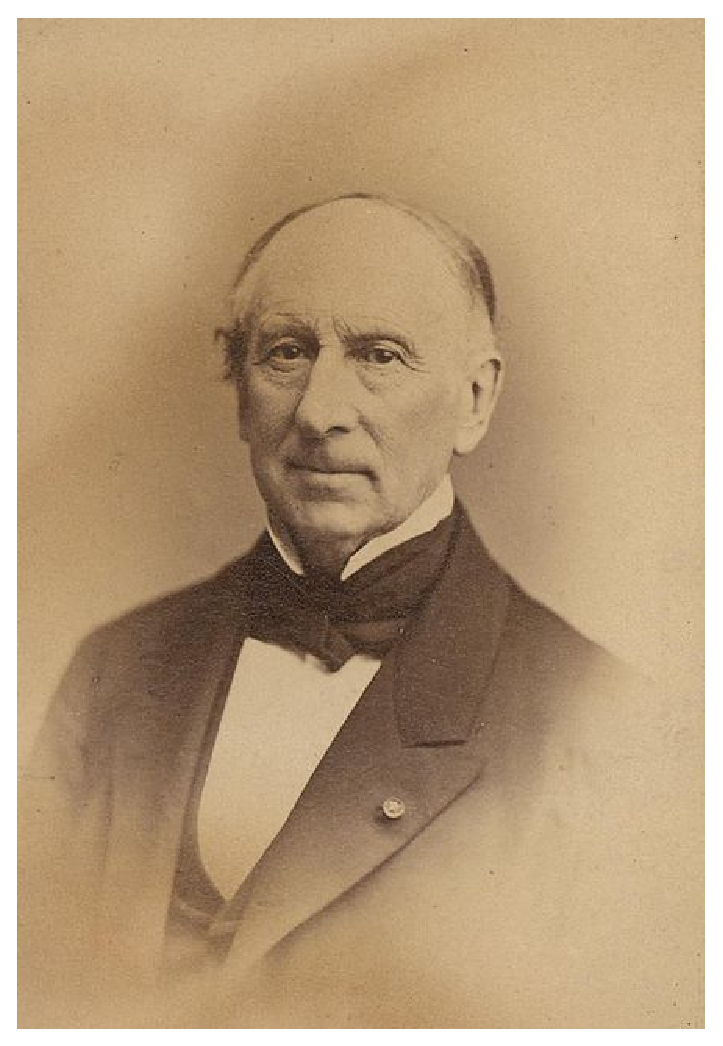
\includegraphics[width=0.9\linewidth]{AugustinCauchy} 
    \caption*{\index{Cauchy, Augustin Louis}\textbf{Augustin Louis Cauchy} 
              (1789-1857), mathématicien français (X1807)}
\end{marginfigure}
%-------------------------------------------------------------------------------
Nous suivrons la présentation \og graphique\fg~ de ce théorème 
et du critère de Nyquist donné par~\cite{reg}. 
%%%%%%%%%%%%%%%%%%%%%%%%%%%%%%%%%%%%%%%%%%%%%%%%%%%%%%%%%%%%%%%%%%%%%%%%%%%%%%%%
\subsection[Image d'un contour d'une fonction de transfert dans $\mathcal{C}$]
{Image d'un contour d'une fonction de transfert dans le plan complexe}
%%%%%%%%%%%%%%%%%%%%%%%%%%%%%%%%%%%%%%%%%%%%%%%%%%%%%%%%%%%%%%%%%%%%%%%%%%%%%%%%
Pour présenter le principe de l'argument de Cauchy, il nous faut déterminer
l'image d'une contour par une fonction de transfert. La~\cref{fig-contour_cauchy} 
présente un exemple de contour  $\mathcal{C}$ parcourant le plan complexe de
la variable $p$ dans le sens des aiguilles d'une montre. On se donne une fonction
de transfert ne possédant aucun pôles et zéros sur $\mathcal{C}$, mais ils
peuvent être contenus dans celui-ci. On appelle $\Gamma$ l'image de 
$\mathcal{C}$ par $F(p)$. \textbf{Le principe de Cauchy nous permet de quantifier le 
nombre de pôles et zéros contenus dans le contour en étudiant l'image de la 
fonction de transfert par ce contour.}
%-------------------------------------------------------------------------------
\begin{figure}[!h]
    \centering
    \tikzsetnextfilename{nyquist_cauchy-chap_stab-ext}
    \begin{tikzpicture}
\begin{axis}
    [
    name=nyy1,
    height=8cm,
    width=8cm,
    axis lines = center,
    ticks=none,
    axis line style = thick,
    enlargelimits=false,
    xlabel=$\Re{p}$,
    ylabel=$\Im{p}$,
    xlabel style={below},
    ylabel style={left},
    ymin=-4,
    ymax=4,
    xmin=-8,
    xmax=8
    ]     
    \pgfmathsetseed{3}
    \draw[
        decoration={markings,mark=at position 0.2 with 
        {\arrow[line width=2pt]{latex}}},
        decoration={markings,mark=at position 0.6 with 
        {\arrow[line width=2pt]{latex}}},
           postaction={decorate},
           thick,
           col4,
           smooth cycle,
           samples=11,
           domain={11:1},
           xshift=3cm,
           yshift=3cm] plot (\x*360/11+5*rnd:1.25cm+0.75cm*rnd) ;
    \node[col4] (ct) at (axis cs:-4,2) {\Large$\mathcal{C}$};
    \addplot[mark=x,ultra thick,only marks,mark size=5pt] 
    coordinates{ (-3.0,-0.5) (-6,-1)};
    \addplot[mark=o,ultra thick,only marks,mark size=5pt] 
    coordinates{ (1,0) (-1,1.2) (-2.1,-1.7) };
\end{axis}
\begin{axis}
    [
    at={(nyy1.south east)},xshift=4ex,
    height=8cm,
    width=8cm,
    axis lines = center,
    ticks=none,
    axis line style = thick,
    enlargelimits=false,
    xlabel=$\Re{F(p)}$,
    ylabel=$\Im{F(p)}$,
    xlabel style={below},
    ylabel style={left},
    ymin=-4,
    ymax=4,
    xmin=-4,
    xmax=4
    ]     
    \def\m{1.0}
    \def\n{2.1}
    \addplot[
    decoration={markings,mark=at position 0.1 with 
    {\arrowreversed[line width=2pt]{latex}}},
    decoration={markings,mark=at position 0.5 with 
    {\arrowreversed[line width=2pt]{latex}}},
    postaction={decorate},
    col1,
    thick,
    domain=1:3,
    samples=50,
    smooth cycle] coordinates 
    {(1.9,-1.5) (0,-2) (-0.75,0.35) (0.25,1.25) (1,0.25) (-0.25,-0.75) 
    (-1.1,-1.25) (-1.5,-1) (-2,0) (-1.5,1.5)  (0,2)  (0.75,1.9) (2,0)}; 
    \node[col1] (ct) at (axis cs:-2.5,2) {\Large$\Gamma:F(\mathcal{C})$};
    \draw[draw=none,fill=black] (axis cs:0,0) circle[radius=2pt];
\end{axis}
\end{tikzpicture}

    \caption{Représentation de la transformation (à gauche) d'un contour $\mathcal{C}$ 
             (à droite) en son image par une fonction analytique $F(p)$. La carte 
             des pôles et zéros est également représentée sur le plan complexe de gauche.
    \label{fig-contour_cauchy}}
\end{figure}
%-------------------------------------------------------------------------------
L'\cref{annexe-cauchy} présente un 

%%%%%%%%%%%%%%%%%%%%%%%%%%%%%%%%%%%%%%%%%%%%%%%%%%%%%%%%%%%%%%%%%%%%%%%%%%%%%%%%
\subsection{Principe de l'argument de Cauchy}
%%%%%%%%%%%%%%%%%%%%%%%%%%%%%%%%%%%%%%%%%%%%%%%%%%%%%%%%%%%%%%%%%%%%%%%%%%%%%%%%
Soit un contour $\mathcal{C}$ parcourant le plan complexe de 
la variable $p$ dans le sens des aiguilles d'une montre et $F(p)$ une fonction 
rationnelle ne possédant ni pôle ni zéro sur $\mathcal{C}$. Le théorème du 
principe de l'argument de Cauchy permet de relier, le nombre de pôles $P$ et 
de zéros $Z$ entourées par le contour $\mathcal{C}$ au comportement de la 
courbe $F(\mathcal{C})$ image $F(p)$ de $\mathcal{C}$.

\begin{theorem}{\'Enoncé du principe de l'argument de Cauchy
    \index{Principe de l'argument de Cauchy}} 
    Si un contour $\mathcal{C}$ contient $Z$ zéros et $P$ pôles d'une fonction 
    analytique $F(p)$ sans en traverser aucun, alors quand on le parcourt dans 
    le sens anti-trigonométrique, le contour $\Gamma=F(\mathcal{C})$ fait un 
    nombre de tours $N$ autour de l'origine dans le sens trigonométrique égal 
    à,
    \[ 
        N=Z-P
    \]
\end{theorem}
On se rapportera à la~\cref{fig-contour_cauchy} pour un exemple d'application 
de ce principe. Dans cet exemple la fonction analytique $F(p)$ possède 2 pôles 
et 3 zéros. Le contour entoure $Z=3$ zéros et $P=1$ pôle.
Le contour $\Gamma=F(\mathcal{C})$ fait alors $N=Z-P=2$ tours autour 
de l'origine dans le sens trigonométrique ($N>0$). Remarquons que les tours 
sont comptés positivement dans le sens trigonométrique (c.f~\cref{fig-ntours}).
%-------------------------------------------------------------------------------
\begin{figure}[!h]
    \centering
    \tikzsetnextfilename{nyquist_ntours_1-chap_stab-ext}
    \input{tikz/nyquist_ntours_1-chap_stab.tex}
    \tikzsetnextfilename{nyquist_ntours_2-chap_stab-ext}
    \input{tikz/nyquist_ntours_2-chap_stab.tex}
    \tikzsetnextfilename{nyquist_ntours_3-chap_stab-ext}
    \begin{tikzpicture}
\begin{axis}[ticks=none,
axis line style = thick,
axis lines = center,
height=4.8cm,
width=4.8cm,
ymin=-1.4,
ymax=1.4,
xmin=-1.4,
xmax=1.4,
clip=false]
\addplot[thick,col4,domain=0:360,samples=100,
decoration={markings,
            mark=at position 0.10 with {\arrowreversed[line width=1pt]{latex}}},
decoration={markings,
            mark=at position 0.20 with {\arrowreversed[line width=1pt]{latex}}},
decoration={markings,
            mark=at position 0.30 with {\arrowreversed[line width=1pt]{latex}}},
decoration={markings,
            mark=at position 0.43 with {\arrowreversed[line width=1pt]{latex}}},
decoration={markings,
            mark=at position 0.50 with {\arrowreversed[line width=1pt]{latex}}},
decoration={markings,
            mark=at position 0.60 with {\arrowreversed[line width=1pt]{latex}}},
decoration={markings,
            mark=at position 0.70 with {\arrowreversed[line width=1pt]{latex}}},
decoration={markings,
            mark=at position 0.80 with {\arrowreversed[line width=1pt]{latex}}},
decoration={markings,
            mark=at position 0.90 with {\arrowreversed[line width=1pt]{latex}}},
postaction={decorate},
] 
({1.0*cos(x)},{1.0*sin(x)});
    \draw[draw=none,fill=black] (axis cs:0.0,0.0) circle[radius=2pt];
\node[below] at (axis cs:0,-1.4) {$N=-1$};
\end{axis}
\end{tikzpicture}


    \tikzsetnextfilename{nyquist_ntours_4-chap_stab-ext}
    \input{tikz/nyquist_ntours_4-chap_stab.tex}
    \tikzsetnextfilename{nyquist_ntours_5-chap_stab-ext}
    \begin{tikzpicture}
\begin{axis}[ticks=none,
axis line style = thick,
axis lines = center,
height=4.8cm,
width=4.8cm,
ymin=-1.4,
ymax=1.4,
xmin=-1.4,
xmax=1.4,
clip=false]
\addplot[thick,col1,domain=0:360,
decoration={markings,mark=at position 0.10 with{\arrow[line width=1pt]{latex}}},
decoration={markings,mark=at position 0.20 with{\arrow[line width=1pt]{latex}}},
decoration={markings,mark=at position 0.30 with{\arrow[line width=1pt]{latex}}},
decoration={markings,mark=at position 0.43 with{\arrow[line width=1pt]{latex}}},
decoration={markings,mark=at position 0.50 with{\arrow[line width=1pt]{latex}}},
decoration={markings,mark=at position 0.60 with{\arrow[line width=1pt]{latex}}},
decoration={markings,mark=at position 0.70 with{\arrow[line width=1pt]{latex}}},
decoration={markings,mark=at position 0.80 with{\arrow[line width=1pt]{latex}}},
decoration={markings,mark=at position 0.90 with{\arrow[line width=1pt]{latex}}},
postaction={decorate},
] coordinates {
({1.0*cos(0)},{1.0*sin(0)})
({0.9994*cos(1)},{0.9994*sin(1)})
({0.9988003599999999*cos(2)},{0.9988003599999999*sin(2)})
({0.9982010797839999*cos(3)},{0.9982010797839999*sin(3)})
({0.9976021591361294*cos(4)},{0.9976021591361294*sin(4)})
({0.9970035978406476*cos(5)},{0.9970035978406476*sin(5)})
({0.9964053956819432*cos(6)},{0.9964053956819432*sin(6)})
({0.995807552444534*cos(7)},{0.995807552444534*sin(7)})
({0.9952100679130672*cos(8)},{0.9952100679130672*sin(8)})
({0.9946129418723193*cos(9)},{0.9946129418723193*sin(9)})
({0.9940161741071959*cos(10)},{0.9940161741071959*sin(10)})
({0.9934197644027315*cos(11)},{0.9934197644027315*sin(11)})
({0.9928237125440899*cos(12)},{0.9928237125440899*sin(12)})
({0.9922280183165634*cos(13)},{0.9922280183165634*sin(13)})
({0.9916326815055734*cos(14)},{0.9916326815055734*sin(14)})
({0.99103770189667*cos(15)},{0.99103770189667*sin(15)})
({0.9904430792755319*cos(16)},{0.9904430792755319*sin(16)})
({0.9898488134279665*cos(17)},{0.9898488134279665*sin(17)})
({0.9892549041399097*cos(18)},{0.9892549041399097*sin(18)})
({0.9886613511974257*cos(19)},{0.9886613511974257*sin(19)})
({0.9880681543867073*cos(20)},{0.9880681543867073*sin(20)})
({0.9874753134940751*cos(21)},{0.9874753134940751*sin(21)})
({0.9868828283059786*cos(22)},{0.9868828283059786*sin(22)})
({0.986290698608995*cos(23)},{0.986290698608995*sin(23)})
({0.9856989241898295*cos(24)},{0.9856989241898295*sin(24)})
({0.9851075048353156*cos(25)},{0.9851075048353156*sin(25)})
({0.9845164403324144*cos(26)},{0.9845164403324144*sin(26)})
({0.9839257304682149*cos(27)},{0.9839257304682149*sin(27)})
({0.9833353750299338*cos(28)},{0.9833353750299338*sin(28)})
({0.9827453738049159*cos(29)},{0.9827453738049159*sin(29)})
({0.9821557265806329*cos(30)},{0.9821557265806329*sin(30)})
({0.9815664331446845*cos(31)},{0.9815664331446845*sin(31)})
({0.9809774932847977*cos(32)},{0.9809774932847977*sin(32)})
({0.9803889067888267*cos(33)},{0.9803889067888267*sin(33)})
({0.9798006734447534*cos(34)},{0.9798006734447534*sin(34)})
({0.9792127930406865*cos(35)},{0.9792127930406865*sin(35)})
({0.978625265364862*cos(36)},{0.978625265364862*sin(36)})
({0.9780380902056431*cos(37)},{0.9780380902056431*sin(37)})
({0.9774512673515197*cos(38)},{0.9774512673515197*sin(38)})
({0.9768647965911087*cos(39)},{0.9768647965911087*sin(39)})
({0.976278677713154*cos(40)},{0.976278677713154*sin(40)})
({0.9756929105065261*cos(41)},{0.9756929105065261*sin(41)})
({0.9751074947602221*cos(42)},{0.9751074947602221*sin(42)})
({0.9745224302633659*cos(43)},{0.9745224302633659*sin(43)})
({0.9739377168052079*cos(44)},{0.9739377168052079*sin(44)})
({0.9733533541751247*cos(45)},{0.9733533541751247*sin(45)})
({0.9727693421626196*cos(46)},{0.9727693421626196*sin(46)})
({0.9721856805573219*cos(47)},{0.9721856805573219*sin(47)})
({0.9716023691489875*cos(48)},{0.9716023691489875*sin(48)})
({0.9710194077274981*cos(49)},{0.9710194077274981*sin(49)})
({0.9704367960828615*cos(50)},{0.9704367960828615*sin(50)})
({0.9698545340052117*cos(51)},{0.9698545340052117*sin(51)})
({0.9692726212848085*cos(52)},{0.9692726212848085*sin(52)})
({0.9686910577120376*cos(53)},{0.9686910577120376*sin(53)})
({0.9681098430774103*cos(54)},{0.9681098430774103*sin(54)})
({0.9675289771715638*cos(55)},{0.9675289771715638*sin(55)})
({0.9669484597852609*cos(56)},{0.9669484597852609*sin(56)})
({0.9663682907093897*cos(57)},{0.9663682907093897*sin(57)})
({0.965788469734964*cos(58)},{0.965788469734964*sin(58)})
({0.965208996653123*cos(59)},{0.965208996653123*sin(59)})
({0.9646298712551311*cos(60)},{0.9646298712551311*sin(60)})
({0.964051093332378*cos(61)},{0.964051093332378*sin(61)})
({0.9634726626763785*cos(62)},{0.9634726626763785*sin(62)})
({0.9628945790787726*cos(63)},{0.9628945790787726*sin(63)})
({0.9623168423313253*cos(64)},{0.9623168423313253*sin(64)})
({0.9617394522259265*cos(65)},{0.9617394522259265*sin(65)})
({0.9611624085545909*cos(66)},{0.9611624085545909*sin(66)})
({0.9605857111094581*cos(67)},{0.9605857111094581*sin(67)})
({0.9600093596827924*cos(68)},{0.9600093596827924*sin(68)})
({0.9594333540669827*cos(69)},{0.9594333540669827*sin(69)})
({0.9588576940545425*cos(70)},{0.9588576940545425*sin(70)})
({0.9582823794381097*cos(71)},{0.9582823794381097*sin(71)})
({0.9577074100104468*cos(72)},{0.9577074100104468*sin(72)})
({0.9571327855644405*cos(73)},{0.9571327855644405*sin(73)})
({0.9565585058931018*cos(74)},{0.9565585058931018*sin(74)})
({0.9559845707895659*cos(75)},{0.9559845707895659*sin(75)})
({0.9554109800470921*cos(76)},{0.9554109800470921*sin(76)})
({0.9548377334590639*cos(77)},{0.9548377334590639*sin(77)})
({0.9542648308189884*cos(78)},{0.9542648308189884*sin(78)})
({0.953692271920497*cos(79)},{0.953692271920497*sin(79)})
({0.9531200565573447*cos(80)},{0.9531200565573447*sin(80)})
({0.9525481845234102*cos(81)},{0.9525481845234102*sin(81)})
({0.9519766556126961*cos(82)},{0.9519766556126961*sin(82)})
({0.9514054696193284*cos(83)},{0.9514054696193284*sin(83)})
({0.9508346263375568*cos(84)},{0.9508346263375568*sin(84)})
({0.9502641255617542*cos(85)},{0.9502641255617542*sin(85)})
({0.9496939670864171*cos(86)},{0.9496939670864171*sin(86)})
({0.9491241507061652*cos(87)},{0.9491241507061652*sin(87)})
({0.9485546762157414*cos(88)},{0.9485546762157414*sin(88)})
({0.947985543410012*cos(89)},{0.947985543410012*sin(89)})
({0.9474167520839659*cos(90)},{0.9474167520839659*sin(90)})
({0.9468483020327155*cos(91)},{0.9468483020327155*sin(91)})
({0.9462801930514959*cos(92)},{0.9462801930514959*sin(92)})
({0.945712424935665*cos(93)},{0.945712424935665*sin(93)})
({0.9451449974807036*cos(94)},{0.9451449974807036*sin(94)})
({0.9445779104822151*cos(95)},{0.9445779104822151*sin(95)})
({0.9440111637359256*cos(96)},{0.9440111637359256*sin(96)})
({0.943444757037684*cos(97)},{0.943444757037684*sin(97)})
({0.9428786901834614*cos(98)},{0.9428786901834614*sin(98)})
({0.9423129629693513*cos(99)},{0.9423129629693513*sin(99)})
({0.9417475751915696*cos(100)},{0.9417475751915696*sin(100)})
({0.9411825266464546*cos(101)},{0.9411825266464546*sin(101)})
({0.9406178171304668*cos(102)},{0.9406178171304668*sin(102)})
({0.9400534464401884*cos(103)},{0.9400534464401884*sin(103)})
({0.9394894143723242*cos(104)},{0.9394894143723242*sin(104)})
({0.9389257207237008*cos(105)},{0.9389257207237008*sin(105)})
({0.9383623652912666*cos(106)},{0.9383623652912666*sin(106)})
({0.9377993478720918*cos(107)},{0.9377993478720918*sin(107)})
({0.9372366682633686*cos(108)},{0.9372366682633686*sin(108)})
({0.9366743262624105*cos(109)},{0.9366743262624105*sin(109)})
({0.936112321666653*cos(110)},{0.936112321666653*sin(110)})
({0.935550654273653*cos(111)},{0.935550654273653*sin(111)})
({0.9349893238810888*cos(112)},{0.9349893238810888*sin(112)})
({0.9344283302867601*cos(113)},{0.9344283302867601*sin(113)})
({0.933867673288588*cos(114)},{0.933867673288588*sin(114)})
({0.9333073526846148*cos(115)},{0.9333073526846148*sin(115)})
({0.9327473682730041*cos(116)},{0.9327473682730041*sin(116)})
({0.9321877198520402*cos(117)},{0.9321877198520402*sin(117)})
({0.931628407220129*cos(118)},{0.931628407220129*sin(118)})
({0.9310694301757968*cos(119)},{0.9310694301757968*sin(119)})
({0.9305107885176913*cos(120)},{0.9305107885176913*sin(120)})
({0.9287428180195076*cos(121)},{0.9287428180195076*sin(121)})
({0.9269782066652705*cos(122)},{0.9269782066652705*sin(122)})
({0.9252169480726065*cos(123)},{0.9252169480726065*sin(123)})
({0.9234590358712685*cos(124)},{0.9234590358712685*sin(124)})
({0.9217044637031131*cos(125)},{0.9217044637031131*sin(125)})
({0.9199532252220771*cos(126)},{0.9199532252220771*sin(126)})
({0.9182053140941552*cos(127)},{0.9182053140941552*sin(127)})
({0.9164607239973763*cos(128)},{0.9164607239973763*sin(128)})
({0.9147194486217813*cos(129)},{0.9147194486217813*sin(129)})
({0.9129814816694*cos(130)},{0.9129814816694*sin(130)})
({0.911246816854228*cos(131)},{0.911246816854228*sin(131)})
({0.909515447902205*cos(132)},{0.909515447902205*sin(132)})
({0.9077873685511908*cos(133)},{0.9077873685511908*sin(133)})
({0.9060625725509436*cos(134)},{0.9060625725509436*sin(134)})
({0.9043410536630968*cos(135)},{0.9043410536630968*sin(135)})
({0.902622805661137*cos(136)},{0.902622805661137*sin(136)})
({0.9009078223303808*cos(137)},{0.9009078223303808*sin(137)})
({0.899196097467953*cos(138)},{0.899196097467953*sin(138)})
({0.8974876248827639*cos(139)},{0.8974876248827639*sin(139)})
({0.8957823983954867*cos(140)},{0.8957823983954867*sin(140)})
({0.8940804118385353*cos(141)},{0.8940804118385353*sin(141)})
({0.892381659056042*cos(142)},{0.892381659056042*sin(142)})
({0.8906861339038356*cos(143)},{0.8906861339038356*sin(143)})
({0.8889938302494182*cos(144)},{0.8889938302494182*sin(144)})
({0.8873047419719443*cos(145)},{0.8873047419719443*sin(145)})
({0.8856188629621976*cos(146)},{0.8856188629621976*sin(146)})
({0.8839361871225694*cos(147)},{0.8839361871225694*sin(147)})
({0.8822567083670365*cos(148)},{0.8822567083670365*sin(148)})
({0.8805804206211392*cos(149)},{0.8805804206211392*sin(149)})
({0.878907317821959*cos(150)},{0.878907317821959*sin(150)})
({0.8772373939180972*cos(151)},{0.8772373939180972*sin(151)})
({0.8755706428696528*cos(152)},{0.8755706428696528*sin(152)})
({0.8739070586482005*cos(153)},{0.8739070586482005*sin(153)})
({0.8722466352367689*cos(154)},{0.8722466352367689*sin(154)})
({0.870589366629819*cos(155)},{0.870589366629819*sin(155)})
({0.8689352468332223*cos(156)},{0.8689352468332223*sin(156)})
({0.8672842698642392*cos(157)},{0.8672842698642392*sin(157)})
({0.8656364297514971*cos(158)},{0.8656364297514971*sin(158)})
({0.8639917205349693*cos(159)},{0.8639917205349693*sin(159)})
({0.8623501362659528*cos(160)},{0.8623501362659528*sin(160)})
({0.8607116710070475*cos(161)},{0.8607116710070475*sin(161)})
({0.8590763188321341*cos(162)},{0.8590763188321341*sin(162)})
({0.857444073826353*cos(163)},{0.857444073826353*sin(163)})
({0.8558149300860829*cos(164)},{0.8558149300860829*sin(164)})
({0.8541888817189193*cos(165)},{0.8541888817189193*sin(165)})
({0.8525659228436533*cos(166)},{0.8525659228436533*sin(166)})
({0.8509460475902504*cos(167)},{0.8509460475902504*sin(167)})
({0.8493292500998288*cos(168)},{0.8493292500998288*sin(168)})
({0.8477155245246392*cos(169)},{0.8477155245246392*sin(169)})
({0.8461048650280424*cos(170)},{0.8461048650280424*sin(170)})
({0.8444972657844891*cos(171)},{0.8444972657844891*sin(171)})
({0.8428927209794986*cos(172)},{0.8428927209794986*sin(172)})
({0.8412912248096376*cos(173)},{0.8412912248096376*sin(173)})
({0.8396927714824992*cos(174)},{0.8396927714824992*sin(174)})
({0.8380973552166825*cos(175)},{0.8380973552166825*sin(175)})
({0.8365049702417708*cos(176)},{0.8365049702417708*sin(176)})
({0.8349156107983114*cos(177)},{0.8349156107983114*sin(177)})
({0.8333292711377946*cos(178)},{0.8333292711377946*sin(178)})
({0.8317459455226328*cos(179)},{0.8317459455226328*sin(179)})
({0.8301656282261398*cos(180)},{0.8301656282261398*sin(180)})
({0.8285883135325102*cos(181)},{0.8285883135325102*sin(181)})
({0.8270139957367983*cos(182)},{0.8270139957367983*sin(182)})
({0.8254426691448984*cos(183)},{0.8254426691448984*sin(183)})
({0.8238743280735231*cos(184)},{0.8238743280735231*sin(184)})
({0.8223089668501834*cos(185)},{0.8223089668501834*sin(185)})
({0.820746579813168*cos(186)},{0.820746579813168*sin(186)})
({0.819187161311523*cos(187)},{0.819187161311523*sin(187)})
({0.8176307057050312*cos(188)},{0.8176307057050312*sin(188)})
({0.8160772073641915*cos(189)},{0.8160772073641915*sin(189)})
({0.8145266606701995*cos(190)},{0.8145266606701995*sin(190)})
({0.8129790600149261*cos(191)},{0.8129790600149261*sin(191)})
({0.8114343998008978*cos(192)},{0.8114343998008978*sin(192)})
({0.8098926744412761*cos(193)},{0.8098926744412761*sin(193)})
({0.8083538783598376*cos(194)},{0.8083538783598376*sin(194)})
({0.8068180059909539*cos(195)},{0.8068180059909539*sin(195)})
({0.8052850517795711*cos(196)},{0.8052850517795711*sin(196)})
({0.8037550101811899*cos(197)},{0.8037550101811899*sin(197)})
({0.8022278756618456*cos(198)},{0.8022278756618456*sin(198)})
({0.8007036426980881*cos(199)},{0.8007036426980881*sin(199)})
({0.7991823057769618*cos(200)},{0.7991823057769618*sin(200)})
({0.7976638593959856*cos(201)},{0.7976638593959856*sin(201)})
({0.7961482980631333*cos(202)},{0.7961482980631333*sin(202)})
({0.7946356162968133*cos(203)},{0.7946356162968133*sin(203)})
({0.7931258086258494*cos(204)},{0.7931258086258494*sin(204)})
({0.7916188695894603*cos(205)},{0.7916188695894603*sin(205)})
({0.7901147937372403*cos(206)},{0.7901147937372403*sin(206)})
({0.7886135756291395*cos(207)},{0.7886135756291395*sin(207)})
({0.7871152098354441*cos(208)},{0.7871152098354441*sin(208)})
({0.7856196909367568*cos(209)},{0.7856196909367568*sin(209)})
({0.784127013523977*cos(210)},{0.784127013523977*sin(210)})
({0.7826371721982814*cos(211)},{0.7826371721982814*sin(211)})
({0.7811501615711047*cos(212)},{0.7811501615711047*sin(212)})
({0.7796659762641196*cos(213)},{0.7796659762641196*sin(213)})
({0.7781846109092178*cos(214)},{0.7781846109092178*sin(214)})
({0.7767060601484902*cos(215)},{0.7767060601484902*sin(215)})
({0.7752303186342081*cos(216)},{0.7752303186342081*sin(216)})
({0.7737573810288031*cos(217)},{0.7737573810288031*sin(217)})
({0.7722872420048483*cos(218)},{0.7722872420048483*sin(218)})
({0.7708198962450391*cos(219)},{0.7708198962450391*sin(219)})
({0.7693553384421735*cos(220)},{0.7693553384421735*sin(220)})
({0.7678935632991334*cos(221)},{0.7678935632991334*sin(221)})
({0.766434565528865*cos(222)},{0.766434565528865*sin(222)})
({0.7649783398543601*cos(223)},{0.7649783398543601*sin(223)})
({0.7635248810086368*cos(224)},{0.7635248810086368*sin(224)})
({0.7620741837347204*cos(225)},{0.7620741837347204*sin(225)})
({0.7606262427856244*cos(226)},{0.7606262427856244*sin(226)})
({0.7591810529243317*cos(227)},{0.7591810529243317*sin(227)})
({0.7577386089237754*cos(228)},{0.7577386089237754*sin(228)})
({0.7562989055668202*cos(229)},{0.7562989055668202*sin(229)})
({0.7548619376462432*cos(230)},{0.7548619376462432*sin(230)})
({0.7534276999647154*cos(231)},{0.7534276999647154*sin(231)})
({0.7519961873347824*cos(232)},{0.7519961873347824*sin(232)})
({0.7505673945788462*cos(233)},{0.7505673945788462*sin(233)})
({0.7491413165291464*cos(234)},{0.7491413165291464*sin(234)})
({0.747717948027741*cos(235)},{0.747717948027741*sin(235)})
({0.7462972839264883*cos(236)},{0.7462972839264883*sin(236)})
({0.744879319087028*cos(237)},{0.744879319087028*sin(237)})
({0.7434640483807626*cos(238)},{0.7434640483807626*sin(238)})
({0.7420514666888391*cos(239)},{0.7420514666888391*sin(239)})
({0.7406415689021303*cos(240)},{0.7406415689021303*sin(240)})
({0.7392343499212163*cos(241)},{0.7392343499212163*sin(241)})
({0.7378298046563659*cos(242)},{0.7378298046563659*sin(242)})
({0.7364279280275189*cos(243)},{0.7364279280275189*sin(243)})
({0.7350287149642666*cos(244)},{0.7350287149642666*sin(244)})
({0.7336321604058345*cos(245)},{0.7336321604058345*sin(245)})
({0.7322382593010633*cos(246)},{0.7322382593010633*sin(246)})
({0.7308470066083913*cos(247)},{0.7308470066083913*sin(247)})
({0.7294583972958354*cos(248)},{0.7294583972958354*sin(248)})
({0.7280724263409732*cos(249)},{0.7280724263409732*sin(249)})
({0.7266890887309254*cos(250)},{0.7266890887309254*sin(250)})
({0.7253083794623366*cos(251)},{0.7253083794623366*sin(251)})
({0.7239302935413582*cos(252)},{0.7239302935413582*sin(252)})
({0.7225548259836296*cos(253)},{0.7225548259836296*sin(253)})
({0.7211819718142607*cos(254)},{0.7211819718142607*sin(254)})
({0.7198117260678136*cos(255)},{0.7198117260678136*sin(255)})
({0.7184440837882847*cos(256)},{0.7184440837882847*sin(256)})
({0.717079040029087*cos(257)},{0.717079040029087*sin(257)})
({0.7157165898530317*cos(258)},{0.7157165898530317*sin(258)})
({0.7143567283323109*cos(259)},{0.7143567283323109*sin(259)})
({0.7129994505484795*cos(260)},{0.7129994505484795*sin(260)})
({0.7116447515924373*cos(261)},{0.7116447515924373*sin(261)})
({0.7102926265644117*cos(262)},{0.7102926265644117*sin(262)})
({0.7089430705739393*cos(263)},{0.7089430705739393*sin(263)})
({0.7075960787398489*cos(264)},{0.7075960787398489*sin(264)})
({0.7062516461902432*cos(265)},{0.7062516461902432*sin(265)})
({0.7049097680624817*cos(266)},{0.7049097680624817*sin(266)})
({0.703570439503163*cos(267)},{0.703570439503163*sin(267)})
({0.702233655668107*cos(268)},{0.702233655668107*sin(268)})
({0.7008994117223376*cos(269)},{0.7008994117223376*sin(269)})
({0.6995677028400652*cos(270)},{0.6995677028400652*sin(270)})
({0.698238524204669*cos(271)},{0.698238524204669*sin(271)})
({0.6969118710086801*cos(272)},{0.6969118710086801*sin(272)})
({0.6955877384537636*cos(273)},{0.6955877384537636*sin(273)})
({0.6942661217507015*cos(274)},{0.6942661217507015*sin(274)})
({0.6929470161193751*cos(275)},{0.6929470161193751*sin(275)})
({0.6916304167887484*cos(276)},{0.6916304167887484*sin(276)})
({0.6903163189968498*cos(277)},{0.6903163189968498*sin(277)})
({0.6890047179907557*cos(278)},{0.6890047179907557*sin(278)})
({0.6876956090265732*cos(279)},{0.6876956090265732*sin(279)})
({0.6863889873694228*cos(280)},{0.6863889873694228*sin(280)})
({0.6850848482934209*cos(281)},{0.6850848482934209*sin(281)})
({0.6837831870816634*cos(282)},{0.6837831870816634*sin(282)})
({0.6824839990262083*cos(283)},{0.6824839990262083*sin(283)})
({0.6811872794280585*cos(284)},{0.6811872794280585*sin(284)})
({0.6798930235971451*cos(285)},{0.6798930235971451*sin(285)})
({0.6786012268523105*cos(286)},{0.6786012268523105*sin(286)})
({0.6773118845212911*cos(287)},{0.6773118845212911*sin(287)})
({0.6760249919407006*cos(288)},{0.6760249919407006*sin(288)})
({0.6747405444560133*cos(289)},{0.6747405444560133*sin(289)})
({0.6734585374215468*cos(290)},{0.6734585374215468*sin(290)})
({0.6721789662004459*cos(291)},{0.6721789662004459*sin(291)})
({0.6709018261646651*cos(292)},{0.6709018261646651*sin(292)})
({0.6696271126949522*cos(293)},{0.6696271126949522*sin(293)})
({0.6683548211808318*cos(294)},{0.6683548211808318*sin(294)})
({0.6670849470205882*cos(295)},{0.6670849470205882*sin(295)})
({0.6658174856212491*cos(296)},{0.6658174856212491*sin(296)})
({0.6645524323985688*cos(297)},{0.6645524323985688*sin(297)})
({0.6632897827770114*cos(298)},{0.6632897827770114*sin(298)})
({0.6620295321897351*cos(299)},{0.6620295321897351*sin(299)})
({0.6607716760785747*cos(300)},{0.6607716760785747*sin(300)})
({0.6595162098940254*cos(301)},{0.6595162098940254*sin(301)})
({0.6582631290952267*cos(302)},{0.6582631290952267*sin(302)})
({0.6570124291499457*cos(303)},{0.6570124291499457*sin(303)})
({0.6557641055345609*cos(304)},{0.6557641055345609*sin(304)})
({0.6545181537340452*cos(305)},{0.6545181537340452*sin(305)})
({0.6532745692419505*cos(306)},{0.6532745692419505*sin(306)})
({0.6520333475603908*cos(307)},{0.6520333475603908*sin(307)})
({0.6507944842000261*cos(308)},{0.6507944842000261*sin(308)})
({0.649557974680046*cos(309)},{0.649557974680046*sin(309)})
({0.6483238145281538*cos(310)},{0.6483238145281538*sin(310)})
({0.6470919992805503*cos(311)},{0.6470919992805503*sin(311)})
({0.6458625244819173*cos(312)},{0.6458625244819173*sin(312)})
({0.6446353856854016*cos(313)},{0.6446353856854016*sin(313)})
({0.6434105784525993*cos(314)},{0.6434105784525993*sin(314)})
({0.6421880983535394*cos(315)},{0.6421880983535394*sin(315)})
({0.6409679409666676*cos(316)},{0.6409679409666676*sin(316)})
({0.639750101878831*cos(317)},{0.639750101878831*sin(317)})
({0.6385345766852611*cos(318)},{0.6385345766852611*sin(318)})
({0.6373213609895592*cos(319)},{0.6373213609895592*sin(319)})
({0.636110450403679*cos(320)},{0.636110450403679*sin(320)})
({0.634901840547912*cos(321)},{0.634901840547912*sin(321)})
({0.633695527050871*cos(322)},{0.633695527050871*sin(322)})
({0.6324915055494743*cos(323)},{0.6324915055494743*sin(323)})
({0.6312897716889303*cos(324)},{0.6312897716889303*sin(324)})
({0.6300903211227213*cos(325)},{0.6300903211227213*sin(325)})
({0.6288931495125881*cos(326)},{0.6288931495125881*sin(326)})
({0.6276982525285142*cos(327)},{0.6276982525285142*sin(327)})
({0.6265056258487101*cos(328)},{0.6265056258487101*sin(328)})
({0.6253152651595975*cos(329)},{0.6253152651595975*sin(329)})
({0.6241271661557942*cos(330)},{0.6241271661557942*sin(330)})
({0.6229413245400982*cos(331)},{0.6229413245400982*sin(331)})
({0.6217577360234721*cos(332)},{0.6217577360234721*sin(332)})
({0.6205763963250275*cos(333)},{0.6205763963250275*sin(333)})
({0.61939730117201*cos(334)},{0.61939730117201*sin(334)})
({0.6182204462997831*cos(335)},{0.6182204462997831*sin(335)})
({0.6170458274518136*cos(336)},{0.6170458274518136*sin(336)})
({0.6158734403796551*cos(337)},{0.6158734403796551*sin(337)})
({0.6147032808429337*cos(338)},{0.6147032808429337*sin(338)})
({0.6135353446093321*cos(339)},{0.6135353446093321*sin(339)})
({0.6123696274545744*cos(340)},{0.6123696274545744*sin(340)})
({0.6112061251624107*cos(341)},{0.6112061251624107*sin(341)})
({0.6100448335246021*cos(342)},{0.6100448335246021*sin(342)})
({0.6088857483409054*cos(343)},{0.6088857483409054*sin(343)})
({0.6077288654190577*cos(344)},{0.6077288654190577*sin(344)})
({0.6065741805747614*cos(345)},{0.6065741805747614*sin(345)})
({0.6054216896316694*cos(346)},{0.6054216896316694*sin(346)})
({0.6042713884213693*cos(347)},{0.6042713884213693*sin(347)})
({0.6031232727833686*cos(348)},{0.6031232727833686*sin(348)})
({0.6019773385650802*cos(349)},{0.6019773385650802*sin(349)})
({0.6008936649799688*cos(-10)},{0.6008936649799688*sin(-10)})
({0.6009537543464668*cos(-9)},{0.6009537543464668*sin(-9)})
({0.6010138497219014*cos(-8)},{0.6010138497219014*sin(-8)})
({0.6010739511068736*cos(-7)},{0.6010739511068736*sin(-7)})
({0.6011340585019842*cos(-6)},{0.6011340585019842*sin(-6)})
({0.6011941719078344*cos(-5)},{0.6011941719078344*sin(-5)})
({0.6012542913250252*cos(-4)},{0.6012542913250252*sin(-4)})
({0.6013144167541576*cos(-3)},{0.6013144167541576*sin(-3)})
({0.601374548195833*cos(-2)},{0.601374548195833*sin(-2)})
({0.6014346856506526*cos(-1)},{0.6014346856506526*sin(-1)})
({0.6014948291192177*cos(0)},{0.6014948291192177*sin(0)})
({0.6015549786021296*cos(1)},{0.6015549786021296*sin(1)})
({0.6016151340999898*cos(2)},{0.6016151340999898*sin(2)})
({0.6016752956133998*cos(3)},{0.6016752956133998*sin(3)})
({0.6017354631429611*cos(4)},{0.6017354631429611*sin(4)})
({0.6017956366892754*cos(5)},{0.6017956366892754*sin(5)})
({0.6018558162529443*cos(6)},{0.6018558162529443*sin(6)})
({0.6019160018345695*cos(7)},{0.6019160018345695*sin(7)})
({0.601976193434753*cos(8)},{0.601976193434753*sin(8)})
({0.6020363910540965*cos(9)},{0.6020363910540965*sin(9)})
({0.6020965946932019*cos(10)},{0.6020965946932019*sin(10)})
({0.6021568043526712*cos(11)},{0.6021568043526712*sin(11)})
({0.6022170200331064*cos(12)},{0.6022170200331064*sin(12)})
({0.6022772417351097*cos(13)},{0.6022772417351097*sin(13)})
({0.6023374694592831*cos(14)},{0.6023374694592831*sin(14)})
({0.6023977032062291*cos(15)},{0.6023977032062291*sin(15)})
({0.6024579429765498*cos(16)},{0.6024579429765498*sin(16)})
({0.6025181887708474*cos(17)},{0.6025181887708474*sin(17)})
({0.6025784405897244*cos(18)},{0.6025784405897244*sin(18)})
({0.6026386984337834*cos(19)},{0.6026386984337834*sin(19)})
({0.6026989623036267*cos(20)},{0.6026989623036267*sin(20)})
({0.602759232199857*cos(21)},{0.602759232199857*sin(21)})
({0.602819508123077*cos(22)},{0.602819508123077*sin(22)})
({0.6028797900738894*cos(23)},{0.6028797900738894*sin(23)})
({0.6029400780528967*cos(24)},{0.6029400780528967*sin(24)})
({0.603000372060702*cos(25)},{0.603000372060702*sin(25)})
({0.603060672097908*cos(26)},{0.603060672097908*sin(26)})
({0.6031209781651178*cos(27)},{0.6031209781651178*sin(27)})
({0.6031812902629343*cos(28)},{0.6031812902629343*sin(28)})
({0.6032416083919606*cos(29)},{0.6032416083919606*sin(29)})
({0.6033019325527998*cos(30)},{0.6033019325527998*sin(30)})
({0.6033622627460551*cos(31)},{0.6033622627460551*sin(31)})
({0.6034225989723296*cos(32)},{0.6034225989723296*sin(32)})
({0.6034829412322269*cos(33)},{0.6034829412322269*sin(33)})
({0.6035432895263502*cos(34)},{0.6035432895263502*sin(34)})
({0.6036036438553029*cos(35)},{0.6036036438553029*sin(35)})
({0.6036640042196884*cos(36)},{0.6036640042196884*sin(36)})
({0.6037243706201103*cos(37)},{0.6037243706201103*sin(37)})
({0.6037847430571723*cos(38)},{0.6037847430571723*sin(38)})
({0.6038451215314781*cos(39)},{0.6038451215314781*sin(39)})
({0.6039055060436312*cos(40)},{0.6039055060436312*sin(40)})
({0.6039658965942356*cos(41)},{0.6039658965942356*sin(41)})
({0.604026293183895*cos(42)},{0.604026293183895*sin(42)})
({0.6040866958132134*cos(43)},{0.6040866958132134*sin(43)})
({0.6041471044827947*cos(44)},{0.6041471044827947*sin(44)})
({0.604207519193243*cos(45)},{0.604207519193243*sin(45)})
({0.6042679399451624*cos(46)},{0.6042679399451624*sin(46)})
({0.6043283667391569*cos(47)},{0.6043283667391569*sin(47)})
({0.6043887995758308*cos(48)},{0.6043887995758308*sin(48)})
({0.6044492384557884*cos(49)},{0.6044492384557884*sin(49)})
({0.604509683379634*cos(50)},{0.604509683379634*sin(50)})
({0.6045701343479719*cos(51)},{0.6045701343479719*sin(51)})
({0.6046305913614067*cos(52)},{0.6046305913614067*sin(52)})
({0.6046910544205428*cos(53)},{0.6046910544205428*sin(53)})
({0.6047515235259848*cos(54)},{0.6047515235259848*sin(54)})
({0.6048119986783375*cos(55)},{0.6048119986783375*sin(55)})
({0.6048724798782052*cos(56)},{0.6048724798782052*sin(56)})
({0.604932967126193*cos(57)},{0.604932967126193*sin(57)})
({0.6049934604229057*cos(58)},{0.6049934604229057*sin(58)})
({0.6050539597689479*cos(59)},{0.6050539597689479*sin(59)})
({0.6051144651649248*cos(60)},{0.6051144651649248*sin(60)})
({0.6051749766114414*cos(61)},{0.6051749766114414*sin(61)})
({0.6052354941091025*cos(62)},{0.6052354941091025*sin(62)})
({0.6052960176585134*cos(63)},{0.6052960176585134*sin(63)})
({0.6053565472602792*cos(64)},{0.6053565472602792*sin(64)})
({0.6054170829150052*cos(65)},{0.6054170829150052*sin(65)})
({0.6054776246232967*cos(66)},{0.6054776246232967*sin(66)})
({0.605538172385759*cos(67)},{0.605538172385759*sin(67)})
({0.6055987262029976*cos(68)},{0.6055987262029976*sin(68)})
({0.6056592860756179*cos(69)},{0.6056592860756179*sin(69)})
({0.6057198520042255*cos(70)},{0.6057198520042255*sin(70)})
({0.6057804239894259*cos(71)},{0.6057804239894259*sin(71)})
({0.6058410020318248*cos(72)},{0.6058410020318248*sin(72)})
({0.6059015861320279*cos(73)},{0.6059015861320279*sin(73)})
({0.6059621762906411*cos(74)},{0.6059621762906411*sin(74)})
({0.6060227725082702*cos(75)},{0.6060227725082702*sin(75)})
({0.606083374785521*cos(76)},{0.606083374785521*sin(76)})
({0.6061439831229996*cos(77)},{0.6061439831229996*sin(77)})
({0.6062045975213118*cos(78)},{0.6062045975213118*sin(78)})
({0.6062652179810639*cos(79)},{0.6062652179810639*sin(79)})
({0.606325844502862*cos(80)},{0.606325844502862*sin(80)})
({0.6063864770873123*cos(81)},{0.6063864770873123*sin(81)})
({0.6064471157350211*cos(82)},{0.6064471157350211*sin(82)})
({0.6065077604465946*cos(83)},{0.6065077604465946*sin(83)})
({0.6065684112226393*cos(84)},{0.6065684112226393*sin(84)})
({0.6066290680637615*cos(85)},{0.6066290680637615*sin(85)})
({0.6066897309705679*cos(86)},{0.6066897309705679*sin(86)})
({0.606750399943665*cos(87)},{0.606750399943665*sin(87)})
({0.6068110749836594*cos(88)},{0.6068110749836594*sin(88)})
({0.6068717560911577*cos(89)},{0.6068717560911577*sin(89)})
({0.6069324432667669*cos(90)},{0.6069324432667669*sin(90)})
({0.6069931365110935*cos(91)},{0.6069931365110935*sin(91)})
({0.6070538358247447*cos(92)},{0.6070538358247447*sin(92)})
({0.6071145412083272*cos(93)},{0.6071145412083272*sin(93)})
({0.607175252662448*cos(94)},{0.607175252662448*sin(94)})
({0.6072359701877142*cos(95)},{0.6072359701877142*sin(95)})
({0.607296693784733*cos(96)},{0.607296693784733*sin(96)})
({0.6073574234541115*cos(97)},{0.6073574234541115*sin(97)})
({0.6074181591964569*cos(98)},{0.6074181591964569*sin(98)})
({0.6074789010123766*cos(99)},{0.6074789010123766*sin(99)})
({0.6075396489024778*cos(100)},{0.6075396489024778*sin(100)})
({0.607600402867368*cos(101)},{0.607600402867368*sin(101)})
({0.6076611629076548*cos(102)},{0.6076611629076548*sin(102)})
({0.6077219290239456*cos(103)},{0.6077219290239456*sin(103)})
({0.607782701216848*cos(104)},{0.607782701216848*sin(104)})
({0.6078434794869696*cos(105)},{0.6078434794869696*sin(105)})
({0.6079042638349182*cos(106)},{0.6079042638349182*sin(106)})
({0.6079650542613018*cos(107)},{0.6079650542613018*sin(107)})
({0.6080258507667279*cos(108)},{0.6080258507667279*sin(108)})
({0.6080866533518046*cos(109)},{0.6080866533518046*sin(109)})
({0.6081474620171398*cos(110)},{0.6081474620171398*sin(110)})
({0.6082082767633414*cos(111)},{0.6082082767633414*sin(111)})
({0.6082690975910178*cos(112)},{0.6082690975910178*sin(112)})
({0.6083299245007768*cos(113)},{0.6083299245007768*sin(113)})
({0.6083907574932269*cos(114)},{0.6083907574932269*sin(114)})
({0.6084515965689762*cos(115)},{0.6084515965689762*sin(115)})
({0.6085124417286331*cos(116)},{0.6085124417286331*sin(116)})
({0.6085732929728059*cos(117)},{0.6085732929728059*sin(117)})
({0.6086341503021032*cos(118)},{0.6086341503021032*sin(118)})
({0.6086950137171334*cos(119)},{0.6086950137171334*sin(119)})
({0.6087558832185052*cos(120)},{0.6087558832185052*sin(120)})
({0.608816758806827*cos(121)},{0.608816758806827*sin(121)})
({0.6088776404827076*cos(122)},{0.6088776404827076*sin(122)})
({0.6089385282467559*cos(123)},{0.6089385282467559*sin(123)})
({0.6089994220995806*cos(124)},{0.6089994220995806*sin(124)})
({0.6090603220417905*cos(125)},{0.6090603220417905*sin(125)})
({0.6091212280739947*cos(126)},{0.6091212280739947*sin(126)})
({0.6091821401968021*cos(127)},{0.6091821401968021*sin(127)})
({0.6092430584108217*cos(128)},{0.6092430584108217*sin(128)})
({0.6093039827166628*cos(129)},{0.6093039827166628*sin(129)})
({0.6093649131149345*cos(130)},{0.6093649131149345*sin(130)})
({0.6094258496062459*cos(131)},{0.6094258496062459*sin(131)})
({0.6094867921912065*cos(132)},{0.6094867921912065*sin(132)})
({0.6095477408704256*cos(133)},{0.6095477408704256*sin(133)})
({0.6096086956445127*cos(134)},{0.6096086956445127*sin(134)})
({0.6096696565140771*cos(135)},{0.6096696565140771*sin(135)})
({0.6097306234797285*cos(136)},{0.6097306234797285*sin(136)})
({0.6097915965420765*cos(137)},{0.6097915965420765*sin(137)})
({0.6098525757017307*cos(138)},{0.6098525757017307*sin(138)})
({0.6099135609593008*cos(139)},{0.6099135609593008*sin(139)})
({0.6099745523153968*cos(140)},{0.6099745523153968*sin(140)})
({0.6100355497706283*cos(141)},{0.6100355497706283*sin(141)})
({0.6100965533256054*cos(142)},{0.6100965533256054*sin(142)})
({0.6101575629809379*cos(143)},{0.6101575629809379*sin(143)})
({0.6102185787372361*cos(144)},{0.6102185787372361*sin(144)})
({0.6102796005951098*cos(145)},{0.6102796005951098*sin(145)})
({0.6103406285551692*cos(146)},{0.6103406285551692*sin(146)})
({0.6104016626180248*cos(147)},{0.6104016626180248*sin(147)})
({0.6104627027842866*cos(148)},{0.6104627027842866*sin(148)})
({0.6105237490545651*cos(149)},{0.6105237490545651*sin(149)})
({0.6105848014294706*cos(150)},{0.6105848014294706*sin(150)})
({0.6106458599096135*cos(151)},{0.6106458599096135*sin(151)})
({0.6107069244956045*cos(152)},{0.6107069244956045*sin(152)})
({0.610767995188054*cos(153)},{0.610767995188054*sin(153)})
({0.6108290719875729*cos(154)},{0.6108290719875729*sin(154)})
({0.6108901548947716*cos(155)},{0.6108901548947716*sin(155)})
({0.6109512439102611*cos(156)},{0.6109512439102611*sin(156)})
({0.6110123390346521*cos(157)},{0.6110123390346521*sin(157)})
({0.6110734402685556*cos(158)},{0.6110734402685556*sin(158)})
({0.6111345476125825*cos(159)},{0.6111345476125825*sin(159)})
({0.6111956610673437*cos(160)},{0.6111956610673437*sin(160)})
({0.6112567806334505*cos(161)},{0.6112567806334505*sin(161)})
({0.6113179063115138*cos(162)},{0.6113179063115138*sin(162)})
({0.611379038102145*cos(163)},{0.611379038102145*sin(163)})
({0.6114401760059552*cos(164)},{0.6114401760059552*sin(164)})
({0.6115013200235558*cos(165)},{0.6115013200235558*sin(165)})
({0.6115624701555582*cos(166)},{0.6115624701555582*sin(166)})
({0.6116236264025737*cos(167)},{0.6116236264025737*sin(167)})
({0.6116847887652139*cos(168)},{0.6116847887652139*sin(168)})
({0.6117459572440904*cos(169)},{0.6117459572440904*sin(169)})
({0.6118071318398148*cos(170)},{0.6118071318398148*sin(170)})
({0.6118683125529988*cos(171)},{0.6118683125529988*sin(171)})
({0.6119294993842541*cos(172)},{0.6119294993842541*sin(172)})
({0.6119906923341926*cos(173)},{0.6119906923341926*sin(173)})
({0.612051891403426*cos(174)},{0.612051891403426*sin(174)})
({0.6121130965925663*cos(175)},{0.6121130965925663*sin(175)})
({0.6121743079022256*cos(176)},{0.6121743079022256*sin(176)})
({0.6122355253330158*cos(177)},{0.6122355253330158*sin(177)})
({0.6122967488855491*cos(178)},{0.6122967488855491*sin(178)})
({0.6123579785604376*cos(179)},{0.6123579785604376*sin(179)})
({0.6124192143582936*cos(180)},{0.6124192143582936*sin(180)})
({0.6140911188134917*cos(181)},{0.6140911188134917*sin(181)})
({0.6157675875678524*cos(182)},{0.6157675875678524*sin(182)})
({0.6174486330819126*cos(183)},{0.6174486330819126*sin(183)})
({0.6191342678502261*cos(184)},{0.6191342678502261*sin(184)})
({0.6208245044014571*cos(185)},{0.6208245044014571*sin(185)})
({0.622519355298473*cos(186)},{0.622519355298473*sin(186)})
({0.6242188331384377*cos(187)},{0.6242188331384377*sin(187)})
({0.6259229505529056*cos(188)},{0.6259229505529056*sin(188)})
({0.6276317202079149*cos(189)},{0.6276317202079149*sin(189)})
({0.6293451548040825*cos(190)},{0.6293451548040825*sin(190)})
({0.6310632670766976*cos(191)},{0.6310632670766976*sin(191)})
({0.6327860697958169*cos(192)},{0.6327860697958169*sin(192)})
({0.6345135757663594*cos(193)},{0.6345135757663594*sin(193)})
({0.6362457978282015*cos(194)},{0.6362457978282015*sin(194)})
({0.6379827488562724*cos(195)},{0.6379827488562724*sin(195)})
({0.6397244417606499*cos(196)},{0.6397244417606499*sin(196)})
({0.6414708894866564*cos(197)},{0.6414708894866564*sin(197)})
({0.6432221050149549*cos(198)},{0.6432221050149549*sin(198)})
({0.6449781013616457*cos(199)},{0.6449781013616457*sin(199)})
({0.646738891578363*cos(200)},{0.646738891578363*sin(200)})
({0.6485044887523718*cos(201)},{0.6485044887523718*sin(201)})
({0.6502749060066657*cos(202)},{0.6502749060066657*sin(202)})
({0.6520501565000638*cos(203)},{0.6520501565000638*sin(203)})
({0.6538302534273089*cos(204)},{0.6538302534273089*sin(204)})
({0.6556152100191655*cos(205)},{0.6556152100191655*sin(205)})
({0.6574050395425177*cos(206)},{0.6574050395425177*sin(206)})
({0.6591997553004687*cos(207)},{0.6591997553004687*sin(207)})
({0.660999370632439*cos(208)},{0.660999370632439*sin(208)})
({0.6628038989142655*cos(209)},{0.6628038989142655*sin(209)})
({0.6646133535583014*cos(210)},{0.6646133535583014*sin(210)})
({0.6664277480135156*cos(211)},{0.6664277480135156*sin(211)})
({0.6682470957655924*cos(212)},{0.6682470957655924*sin(212)})
({0.6700714103370323*cos(213)},{0.6700714103370323*sin(213)})
({0.6719007052872523*cos(214)},{0.6719007052872523*sin(214)})
({0.6737349942126865*cos(215)},{0.6737349942126865*sin(215)})
({0.675574290746887*cos(216)},{0.675574290746887*sin(216)})
({0.677418608560626*cos(217)},{0.677418608560626*sin(217)})
({0.6792679613619964*cos(218)},{0.6792679613619964*sin(218)})
({0.6811223628965146*cos(219)},{0.6811223628965146*sin(219)})
({0.6829818269472221*cos(220)},{0.6829818269472221*sin(220)})
({0.684846367334788*cos(221)},{0.684846367334788*sin(221)})
({0.6867159979176118*cos(222)},{0.6867159979176118*sin(222)})
({0.6885907325919268*cos(223)},{0.6885907325919268*sin(223)})
({0.6904705852919027*cos(224)},{0.6904705852919027*sin(224)})
({0.6923555699897496*cos(225)},{0.6923555699897496*sin(225)})
({0.6942457006958215*cos(226)},{0.6942457006958215*sin(226)})
({0.696140991458721*cos(227)},{0.696140991458721*sin(227)})
({0.6980414563654033*cos(228)},{0.6980414563654033*sin(228)})
({0.6999471095412807*cos(229)},{0.6999471095412807*sin(229)})
({0.7018579651503283*cos(230)},{0.7018579651503283*sin(230)})
({0.7037740373951886*cos(231)},{0.7037740373951886*sin(231)})
({0.7056953405172774*cos(232)},{0.7056953405172774*sin(232)})
({0.7076218887968896*cos(233)},{0.7076218887968896*sin(233)})
({0.709553696553305*cos(234)},{0.709553696553305*sin(234)})
({0.7114907781448955*cos(235)},{0.7114907781448955*sin(235)})
({0.713433147969231*cos(236)},{0.713433147969231*sin(236)})
({0.7153808204631869*cos(237)},{0.7153808204631869*sin(237)})
({0.7173338101030513*cos(238)},{0.7173338101030513*sin(238)})
({0.7192921314046326*cos(239)},{0.7192921314046326*sin(239)})
({0.7212557989233671*cos(240)},{0.7212557989233671*sin(240)})
({0.7232248272544278*cos(241)},{0.7232248272544278*sin(241)})
({0.7251992310328323*cos(242)},{0.7251992310328323*sin(242)})
({0.7271790249335519*cos(243)},{0.7271790249335519*sin(243)})
({0.7291642236716205*cos(244)},{0.7291642236716205*sin(244)})
({0.7311548420022439*cos(245)},{0.7311548420022439*sin(245)})
({0.73315089472091*cos(246)},{0.73315089472091*sin(246)})
({0.735152396663498*cos(247)},{0.735152396663498*sin(247)})
({0.7371593627063893*cos(248)},{0.7371593627063893*sin(248)})
({0.7391718077665776*cos(249)},{0.7391718077665776*sin(249)})
({0.7411897468017803*cos(250)},{0.7411897468017803*sin(250)})
({0.743213194810549*cos(251)},{0.743213194810549*sin(251)})
({0.7452421668323818*cos(252)},{0.7452421668323818*sin(252)})
({0.747276677947834*cos(253)},{0.747276677947834*sin(253)})
({0.7493167432786315*cos(254)},{0.7493167432786315*sin(254)})
({0.751362377987782*cos(255)},{0.751362377987782*sin(255)})
({0.7534135972796886*cos(256)},{0.7534135972796886*sin(256)})
({0.755470416400262*cos(257)},{0.755470416400262*sin(257)})
({0.7575328506370347*cos(258)},{0.7575328506370347*sin(258)})
({0.7596009153192738*cos(259)},{0.7596009153192738*sin(259)})
({0.7616746258180953*cos(260)},{0.7616746258180953*sin(260)})
({0.7637539975465786*cos(261)},{0.7637539975465786*sin(261)})
({0.7658390459598806*cos(262)},{0.7658390459598806*sin(262)})
({0.767929786555351*cos(263)},{0.767929786555351*sin(263)})
({0.7700262348726471*cos(264)},{0.7700262348726471*sin(264)})
({0.7721284064938494*cos(265)},{0.7721284064938494*sin(265)})
({0.7742363170435775*cos(266)},{0.7742363170435775*sin(266)})
({0.7763499821891064*cos(267)},{0.7763499821891064*sin(267)})
({0.7784694176404826*cos(268)},{0.7784694176404826*sin(268)})
({0.7805946391506411*cos(269)},{0.7805946391506411*sin(269)})
({0.7827256625155222*cos(270)},{0.7827256625155222*sin(270)})
({0.7848625035741895*cos(271)},{0.7848625035741895*sin(271)})
({0.787005178208947*cos(272)},{0.787005178208947*sin(272)})
({0.7891537023454573*cos(273)},{0.7891537023454573*sin(273)})
({0.7913080919528603*cos(274)},{0.7913080919528603*sin(274)})
({0.7934683630438916*cos(275)},{0.7934683630438916*sin(275)})
({0.7956345316750013*cos(276)},{0.7956345316750013*sin(276)})
({0.797806613946474*cos(277)},{0.797806613946474*sin(277)})
({0.7999846260025478*cos(278)},{0.7999846260025478*sin(278)})
({0.8021685840315347*cos(279)},{0.8021685840315347*sin(279)})
({0.8043585042659407*cos(280)},{0.8043585042659407*sin(280)})
({0.8065544029825866*cos(281)},{0.8065544029825866*sin(281)})
({0.808756296502729*cos(282)},{0.808756296502729*sin(282)})
({0.8109642011921814*cos(283)},{0.8109642011921814*sin(283)})
({0.813178133461436*cos(284)},{0.813178133461436*sin(284)})
({0.8153981097657856*cos(285)},{0.8153981097657856*sin(285)})
({0.8176241466054461*cos(286)},{0.8176241466054461*sin(286)})
({0.819856260525679*cos(287)},{0.819856260525679*sin(287)})
({0.822094468116914*cos(288)},{0.822094468116914*sin(288)})
({0.8243387860148731*cos(289)},{0.8243387860148731*sin(289)})
({0.8265892309006936*cos(290)},{0.8265892309006936*sin(290)})
({0.8288458195010524*cos(291)},{0.8288458195010524*sin(291)})
({0.8311085685882902*cos(292)},{0.8311085685882902*sin(292)})
({0.8333774949805361*cos(293)},{0.8333774949805361*sin(293)})
({0.8356526155418329*cos(294)},{0.8356526155418329*sin(294)})
({0.837933947182262*cos(295)},{0.837933947182262*sin(295)})
({0.8402215068580695*cos(296)},{0.8402215068580695*sin(296)})
({0.8425153115717919*cos(297)},{0.8425153115717919*sin(297)})
({0.8448153783723829*cos(298)},{0.8448153783723829*sin(298)})
({0.8471217243553394*cos(299)},{0.8471217243553394*sin(299)})
({0.8494343666628293*cos(300)},{0.8494343666628293*sin(300)})
({0.8517533224838187*cos(301)},{0.8517533224838187*sin(301)})
({0.8540786090541995*cos(302)},{0.8540786090541995*sin(302)})
({0.8564102436569174*cos(303)},{0.8564102436569174*sin(303)})
({0.8587482436221007*cos(304)},{0.8587482436221007*sin(304)})
({0.861092626327189*cos(305)},{0.861092626327189*sin(305)})
({0.8634434091970621*cos(306)},{0.8634434091970621*sin(306)})
({0.8658006097041699*cos(307)},{0.8658006097041699*sin(307)})
({0.8681642453686622*cos(308)},{0.8681642453686622*sin(308)})
({0.8705343337585185*cos(309)},{0.8705343337585185*sin(309)})
({0.8729108924896792*cos(310)},{0.8729108924896792*sin(310)})
({0.8752939392261759*cos(311)},{0.8752939392261759*sin(311)})
({0.8776834916802633*cos(312)},{0.8776834916802633*sin(312)})
({0.8800795676125504*cos(313)},{0.8800795676125504*sin(313)})
({0.8824821848321325*cos(314)},{0.8824821848321325*sin(314)})
({0.8848913611967241*cos(315)},{0.8848913611967241*sin(315)})
({0.887307114612791*cos(316)},{0.887307114612791*sin(316)})
({0.8897294630356838*cos(317)},{0.8897294630356838*sin(317)})
({0.8921584244697711*cos(318)},{0.8921584244697711*sin(318)})
({0.8945940169685735*cos(319)},{0.8945940169685735*sin(319)})
({0.8970362586348977*cos(320)},{0.8970362586348977*sin(320)})
({0.8994851676209709*cos(321)},{0.8994851676209709*sin(321)})
({0.901940762128576*cos(322)},{0.901940762128576*sin(322)})
({0.9044030604091869*cos(323)},{0.9044030604091869*sin(323)})
({0.906872080764104*cos(324)},{0.906872080764104*sin(324)})
({0.9093478415445899*cos(325)},{0.9093478415445899*sin(325)})
({0.9118303611520066*cos(326)},{0.9118303611520066*sin(326)})
({0.9143196580379515*cos(327)},{0.9143196580379515*sin(327)})
({0.9168157507043949*cos(328)},{0.9168157507043949*sin(328)})
({0.9193186577038178*cos(329)},{0.9193186577038178*sin(329)})
({0.9218283976393492*cos(330)},{0.9218283976393492*sin(330)})
({0.9243449891649045*cos(331)},{0.9243449891649045*sin(331)})
({0.9268684509853246*cos(332)},{0.9268684509853246*sin(332)})
({0.9293988018565144*cos(333)},{0.9293988018565144*sin(333)})
({0.9319360605855825*cos(334)},{0.9319360605855825*sin(334)})
({0.9344802460309811*cos(335)},{0.9344802460309811*sin(335)})
({0.9370313771026456*cos(336)},{0.9370313771026456*sin(336)})
({0.9395894727621358*cos(337)},{0.9395894727621358*sin(337)})
({0.9421545520227763*cos(338)},{0.9421545520227763*sin(338)})
({0.9447266339497984*cos(339)},{0.9447266339497984*sin(339)})
({0.9473057376604812*cos(340)},{0.9473057376604812*sin(340)})
({0.9498918823242942*cos(341)},{0.9498918823242942*sin(341)})
({0.9524850871630395*cos(342)},{0.9524850871630395*sin(342)})
({0.9550853714509945*cos(343)},{0.9550853714509945*sin(343)})
({0.9576927545150556*cos(344)},{0.9576927545150556*sin(344)})
({0.9603072557348816*cos(345)},{0.9603072557348816*sin(345)})
({0.9629288945430378*cos(346)},{0.9629288945430378*sin(346)})
({0.9655576904251402*cos(347)},{0.9655576904251402*sin(347)})
({0.9681936629200008*cos(348)},{0.9681936629200008*sin(348)})
({0.9708368316197723*cos(349)},{0.9708368316197723*sin(349)})
({0.9734872161700941*cos(350)},{0.9734872161700941*sin(350)})
({0.9761448362702384*cos(351)},{0.9761448362702384*sin(351)})
({0.978809711673256*cos(352)},{0.978809711673256*sin(352)})
({0.9814818621861239*cos(353)},{0.9814818621861239*sin(353)})
({0.9841613076698918*cos(354)},{0.9841613076698918*sin(354)})
({0.9868480680398306*cos(355)},{0.9868480680398306*sin(355)})
({0.9895421632655792*cos(356)},{0.9895421632655792*sin(356)})
({0.9922436133712942*cos(357)},{0.9922436133712942*sin(357)})
({0.9949524384357977*cos(358)},{0.9949524384357977*sin(358)})
({0.9976686585927274*cos(359)},{0.9976686585927274*sin(359)})
({1.0003922940306853*cos(360)},{1.0003922940306853*sin(360)})
};
\draw[draw=none,fill=black] (axis cs:0,0) circle (2pt);
\node[below] at (axis cs:0,-1.4) {$N=2$};
\end{axis}
\end{tikzpicture}

    \tikzsetnextfilename{nyquist_ntours_6-chap_stab-ext}
    \input{tikz/nyquist_ntours_6-chap_stab.tex}
    \caption{Représentation schématique du nombre de tours autour de 
             l'origine de l'image d'une fraction rationnelle d'un contour 
             fermé. Le sens positif est celui du sens trigonométrique.
             \label{fig-ntours}}
\end{figure}
%-------------------------------------------------------------------------------
\clearpage
%%%%%%%%%%%%%%%%%%%%%%%%%%%%%%%%%%%%%%%%%%%%%%%%%%%%%%%%%%%%%%%%%%%%%%%%%%%%%%%%
\subsection{Contours de Nyquist et de Bromwich}
%%%%%%%%%%%%%%%%%%%%%%%%%%%%%%%%%%%%%%%%%%%%%%%%%%%%%%%%%%%%%%%%%%%%%%%%%%%%%%%%
Pour pouvoir appliquer le critère de Nyquist par l'intermédiaire du principe 
de l'argument de Cauchy, il nous faut définir le contour orienté dans le plan 
$p$ qui entoure la zone instable (c.a.d le demi-plan à partie réelle positive).
Nous présentons deux types de contours le contour de Nyquist et ceux de 
Bromwich.
%-------------------------------------------------------------------------------
\begin{marginfigure}
    \centering
    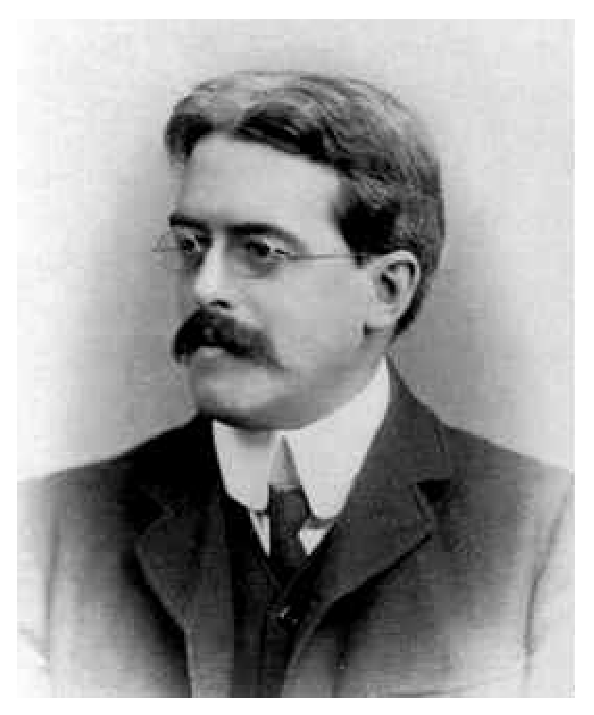
\includegraphics[width=0.9\linewidth]{ThomasBromwich.eps} 
    \caption*{\index{Bromwich, Thomas}\textbf{Thomas John I'Anson Bromwich} 
             (1875-1929), mathématicien anglais.}
\end{marginfigure}
%-------------------------------------------------------------------------------
La~\cref{fig-contours} présente les contours classiques pour l'application 
du critère de Nyquist. Ces contours sont composés de tout l'axe des 
imaginaires, d'un demi cercle de rayon infini centré sur l'origine et dans le
cas où $p=0$ est un pôle ou un zéro de la fonction de transfert en boucle 
ouverte, le contour est également composé d'un cercle de rayon 
$r\rightarrow0$ centré sur les pôles nuls.
%-------------------------------------------------------------------------------
\begin{figure}[!h]
    \centering
    \tikzsetnextfilename{nyquist_contour-chap_stab-ext}
    \begin{tikzpicture}
    \def\rr{1.6}
    \pgfmathsetmacro\ymax{\rr+0.2}
\begin{axis}
    [
    ticks=none,
    axis line style = thick,
    axis lines = center,
    height=6cm,
    width=4cm,
    xlabel=$\Re{p}$,
    ylabel=$\Im{p}$,
    xlabel style={below},
    ylabel style={left,yshift=0.5em},
    ymin=-\ymax,
    ymax=\ymax,
    xmin=-0.8,
    xmax=1.2,
    clip=false]
    \draw[dashed,col1,very thick,-{Latex[length=2.5mm]}] 
    (axis cs:0,-\rr) -- (axis cs:0,-0.8) node[left] {\textbf{III}} ;
    \draw[dashed,col1,very thick,-{Latex[length=2.5mm]}] 
    (axis cs:0,-0.85) -- (axis cs:0,0) ;
    \draw[col1,very thick,-{Latex[length=2.5mm]}] 
    (axis cs:0,0) -- (axis cs:0,0.8) node[left] {\textbf{I}};
    \draw[col1,very thick]                        
    (axis cs:0,0.75) -- (axis cs:0,1.4) ;
    \addplot[col4,very thick,-{Latex[length=2.5mm]},domain=90:60] 
    ({\rr*cos(x)},{\rr*sin(x)});
    \addplot[col4,very thick,domain=62:0] 
    ({\rr*cos(x)},{\rr*sin(x)});
    \addplot[col4,very thick,-{Latex[length=2.5mm]},domain=0:-60] 
    ({\rr*cos(x)},{\rr*sin(x)});
    \addplot[col4,very thick,domain=-58:-90] 
    ({\rr*cos(x)},{\rr*sin(x)});
    \node[right,xshift=0.5em,col4] at 
    (axis cs:{\rr*cos(50)},{\rr*sin(50)}) {\textbf{II}};
    \node[left,col4] at (axis cs:{\rr*cos(90)},{\rr*sin(90)}) 
    {\scriptsize $p\rightarrow+j\infty$};
    \node[left,col4] at (axis cs:{\rr*cos(-90)},{\rr*sin(-90)}) 
    {\scriptsize $p\rightarrow-j\infty$};
    \draw[dashed,thick] (axis cs:0,0) -- 
    (axis cs:{\rr*cos(20)},{\rr*sin(20)}) 
    node[midway,above,yshift=0.5em] {\small$R\rightarrow\infty$};
    \end{axis}
\end{tikzpicture}

    \tikzsetnextfilename{bromwich_contour1-chap_stab-ext}
    \begin{tikzpicture}
    \def\rr{1.6}
    \pgfmathsetmacro\ymax{\rr+0.2}
    \begin{axis}
    [
        ticks=none,
        axis line style = thick,
        axis lines = center,
        height=6cm,
        width=4cm,
        xlabel=$\Re{p}$,
        ylabel=$\Im{p}$,
        xlabel style={below},
        ylabel style={left,yshift=0.5em},
        ymin=-\ymax,
        ymax=\ymax,
        xmin=-0.8,
        xmax=1.2,
        clip=false
    ]
    \draw[dashed,col1,very thick,-{Latex[length=2.5mm]}] 
    (axis cs:0,-1.4) -- (axis cs:0,-0.7) node[left] {\textbf{III}};
    \draw[dashed,col1,very thick] (axis cs:0,-0.75) -- (axis cs:0,-0.15) ;
    \addplot[col3,very thick,domain=-90:-50,samples=10] 
    ({0.15*cos(x)},{0.15*sin(x)});
    \addplot[col3,very thick,domain=-51:-52,samples=10] 
    ({0.15*cos(x)},{0.15*sin(x)});
    \addplot[col3,very thick,domain=-50:60,samples=10] 
    ({0.15*cos(x)},{0.15*sin(x)});
    \addplot[col3,very thick,domain=54:90,samples=10] 
    ({0.15*cos(x)},{0.15*sin(x)});
    \draw[col1,thick,-{Latex[length=2.5mm]}]  
    (axis cs:0,0.15) -- (axis cs:0,0.7) node[left] {\textbf{I}} ;
    \draw[col1,thick]        (axis cs:0,0.65) -- (axis cs:0,\rr) ;
    \addplot[col4,very thick,-{Latex[length=2.5mm]},domain=90:60,samples=50] 
    ({\rr*cos(x)},{\rr*sin(x)});
    \addplot[col4,very thick,-{Latex[length=2.5mm]},domain=62:-60,samples=50] 
    ({\rr*cos(x)},{\rr*sin(x)});
    \addplot[col4,very thick,domain=-58:-90,samples=10] 
    ({\rr*cos(x)},{\rr*sin(x)});
    \node[right,xshift=0.5em,col4] at 
    (axis cs:{\rr*cos(50)},{\rr*sin(50)}) {\textbf{II}};
    \node[right,col3] at 
    (axis cs:{0.20*cos(60)},{0.20*sin(60)}) {\textbf{IV}};
    \node[left,col3] at (axis cs:{-0.15*cos(90)},{0.15*sin(90)}) 
    {\scriptsize $p\rightarrow0^+$};
    \node[left,col3] at (axis cs:{-0.15*cos(-90)},{0.15*sin(-90)}) 
    {\scriptsize $p\rightarrow0^-$};
    \node[left,col4] at (axis cs:{\rr*cos(90)},{\rr*sin(90)}) 
    {\scriptsize $p\rightarrow+j\infty$};
    \node[left,col4] at (axis cs:{\rr*cos(-90)},{\rr*sin(-90)}) 
    {\scriptsize $p\rightarrow-j\infty$};
\end{axis}
\end{tikzpicture}

    \tikzsetnextfilename{bromwich_contour2-chap_stab-ext}
    \begin{tikzpicture}
    \def\rr{1.6}
    \pgfmathsetmacro\ymax{\rr+0.2}
    \begin{axis}[
        ticks=none,
        axis line style = thick,
        axis lines = center,
        height=6cm,
        width=4cm,
        xlabel=$\Re{p}$,
        ylabel=$\Im{p}$,
        xlabel style={below},
        ylabel style={left,yshift=0.5em},
        ymin=-\ymax,
        ymax=\ymax,
        xmin=-0.8,
        xmax=1.2,
        clip=false
    ]
    \draw[col5,thick,-{Latex[length=2.5mm]}] 
    (axis cs:0,-1.4) -- (axis cs:0,-1.0);
    \draw[col5,thick] (axis cs:0,-1.1) -- (axis cs:0,-0.85) ;
    \addplot[col5,very thick,domain=-90:-50,samples=10] 
    ({0.15*cos(x)},{-0.7+0.15*sin(x)});
    \addplot[col5,very thick,domain=-51:-52,samples=10] 
    ({0.15*cos(x)},{-0.7+0.15*sin(x)});
    \addplot[col5,very thick,domain=-50:60,samples=10]  
    ({0.15*cos(x)},{-0.7+0.15*sin(x)});
    \addplot[col5,very thick,domain=54:90,samples=10] 
    ({0.15*cos(x)},{-0.7+0.15*sin(x)});
    \draw[col5,thick,-{Latex[length=2.5mm]}] 
    (axis cs:0,-0.55) -- (axis cs:0,-0.3) ;
    \draw[col5,thick] (axis cs:0,-0.35) -- (axis cs:0,-0.15) ;
    \addplot[col5,very thick,domain=-90:-50,samples=10] 
    ({0.15*cos(x)},{0.15*sin(x)});
    \addplot[col5,very thick,domain=-51:-52,samples=10] 
    ({0.15*cos(x)},{0.15*sin(x)});
    \addplot[col5,very thick,domain=-50:60,samples=10]  
    ({0.15*cos(x)},{0.15*sin(x)});
    \addplot[col5,very thick,domain=54:90,samples=10]   
    ({0.15*cos(x)},{0.15*sin(x)});
    \draw[col5,thick,-{Latex[length=2.5mm]}]    
    (axis cs:0,0.15) -- (axis cs:0,0.4) ;
    \draw[col5,thick]        
    (axis cs:0,0.35) -- (axis cs:0,0.55) ;
    \addplot[col5,very thick,domain=-90:-50,samples=10] 
    ({0.15*cos(x)},{0.7+0.15*sin(x)});
    \addplot[col5,very thick,domain=-51:-52,samples=10] 
    ({0.15*cos(x)},{0.7+0.15*sin(x)});
    \addplot[col5,very thick,domain=-50:60,samples=10]  
    ({0.15*cos(x)},{0.7+0.15*sin(x)});
    \addplot[col5,very thick,domain=54:90,samples=10]   
    ({0.15*cos(x)},{0.7+0.15*sin(x)});
    \draw[col5,thick,-{Latex[length=2.5mm]}]    
    (axis cs:0,0.85) -- (axis cs:0,1.1) ;
    \draw[col5,thick]        (axis cs:0,1.0) -- (axis cs:0,\rr) ;
    \addplot[col5,very thick,-{Latex[length=2.5mm]},domain=90:60,samples=50] 
    ({\rr*cos(x)},{\rr*sin(x)});
    \addplot[col5,very thick,-{Latex[length=2.5mm]},domain=62:-60,samples=50] 
    ({\rr*cos(x)},{\rr*sin(x)});
    \addplot[col5,very thick,domain=-58:-90,samples=10] 
    ({\rr*cos(x)},{\rr*sin(x)});
    \draw[dashed,thick] (axis cs:0,0) -- (axis cs:{\rr*cos(20)},{\rr*sin(20)})
    node[midway,above,yshift=0.5em] {\small$R\rightarrow\infty$};
    \addplot[mark=x,black,ultra thick,only marks,mark size=4pt] 
    coordinates {(0,0) (0,-0.7) (0,0.7)};
    \node[left] at (axis cs:0,0.7) {$p_1$};
    \node[left] at (axis cs:0,-0.7) {$p_2$};
%    \node[below, text width=6cm,text justified,align=center] at 
%    (axis cs:0,-1.6) 
%    {(c) 0, $p_1$ et $p_2$ sont des pôles\\ ou zéros de $H_{BO}$};
    %\draw[green,ultra thick] (axis cs:0,0) circle[radius=1.9cm];
    \end{axis}
\end{tikzpicture}

    \caption{(a) Contour de Nyquist :  $H_{BO}$ ne possède aucun pôle ou zéro 
             et contours de Bromwich: (b) 0 est un pôle\\ ou zéro de $H_{BO}$
             (c) 0, $p_1$ et $p_2$ sont des pôles\\ ou zéros de $H_{BO}$.
             \label{fig-contours}} 
\end{figure}
%-------------------------------------------------------------------------------
%%%%%%%%%%%%%%%%%%%%%%%%%%%%%%%%%%%%%%%%%%%%%%%%%%%%%%%%%%%%%%%%%%%%%%%%%%%%%%%%
\paragraph{Contour de Nyquist}
%%%%%%%%%%%%%%%%%%%%%%%%%%%%%%%%%%%%%%%%%%%%%%%%%%%%%%%%%%%%%%%%%%%%%%%%%%%%%%%%
La~\cref{fig-contours} (a) présente le contour de Nyquist. Celui-ci est 
composé de 3 portions:
%-------------------------------------------------------------------------------
\begin{itemize}
    \item \textbf{I} : l'axe des imaginaires positifs pour laquelle $p=\jw$ 
          avec $\omega\in[0,\infty[$,
    \item \textbf{II}: un demi-cercle de rayon $R$ entourant tout le 
          demi-plan complexe de partie réelle positive et pour lequel 
          $p=Re^{j\theta}$ avec $R\rightarrow\infty$ et $\theta\in[0,\pi/2]$,
    \item \textbf{III}: l'axe des imaginaires négatifs  pour laquelle $p=-\jw$ 
          avec $\omega\in]-\infty,0]$, symétrique de \textbf{I}
\end{itemize}
%-------------------------------------------------------------------------------
%La courbe image d'une fonction de transfert $H_{BO}(p)$
%en boucle ouverte de ces deux portions. 
L'image de la portion \textbf{I} est donné par 
$H_{BO}(\boldsymbol{\mathrm{I}})=H_{BO}(\jw)$, ce qui correspond au lieu de 
Nyquist pour $\omega\in[0,\infty[$. L'image de la portion \textbf{II} est 
l'origine du plan en 0. L'image de la portion \textbf{III} peut être 
déterminé à partir de l'image de la portion \textbf{I} par symétrie par 
rapport à l'axe des réels\footnote{On notera en effet que 
$H_{BO}(-\jw)=\Re{H_{BO}(\jw)}-\Im{H_{BO}(\jw)}$}.
%%%%%%%%%%%%%%%%%%%%%%%%%%%%%%%%%%%%%%%%%%%%%%%%%%%%%%%%%%%%%%%%%%%%%%%%%%%%%%%%
\paragraph{Exemple}
%%%%%%%%%%%%%%%%%%%%%%%%%%%%%%%%%%%%%%%%%%%%%%%%%%%%%%%%%%%%%%%%%%%%%%%%%%%%%%%%
Déterminons l'image par le contour de Bromwich de la fonction de transfert 
suivante : $H_1(p)=\dfrac{1}{1+p}$
%-------------------------------------------------------------------------------
\begin{figure}[!h]
    \centering
    \tikzsetnextfilename{nyquist_contours_exemple_1-chap_stab-ext}
    \begin{tikzpicture}
\begin{axis}
    [
    name=aaa1,
    ticks=none,
    axis line style = thick,
    axis lines = center,
    height=6cm,
    width=6cm,
    xlabel=$\Re{p}$,
    ylabel=$\Im{p}$,
    xlabel style={below},
    ylabel style={left,yshift=0.5em},
    ymin=-1.6,
    ymax=1.6,
    xmin=-0.8,
    xmax=2.4,
    clip=false]
    \draw[dashed,col1,very thick,-{Latex[length=2.5mm]}] 
    (axis cs:0,-1.4) -- (axis cs:0,-0.8) node[left] {\textbf{III}} ;
    \draw[dashed,col1,very thick,-{Latex[length=2.5mm]}] 
    (axis cs:0,-0.85) -- (axis cs:0,0) ;
    \draw[col1,very thick,-{Latex[length=2.5mm]}] 
    (axis cs:0,0) -- (axis cs:0,0.8) node[left] {\textbf{I}};
    \draw[col1,very thick]                        
    (axis cs:0,0.75) -- (axis cs:0,1.4) ;
    \addplot[col4,very thick,-{Latex[length=2.5mm]},domain=90:60] 
    ({1.4*cos(x)},{1.4*sin(x)});
    \addplot[col4,very thick,domain=62:0] 
    ({1.4*cos(x)},{1.4*sin(x)});
    \addplot[col4,very thick,-{Latex[length=2.5mm]},domain=0:-60] 
    ({1.4*cos(x)},{1.4*sin(x)});
    \addplot[col4,very thick,domain=-58:-90] 
    ({1.4*cos(x)},{1.4*sin(x)});
    \node[right,xshift=0.5em,col4] at 
    (axis cs:{1.4*cos(50)},{1.4*sin(50)}) {\textbf{II}};
    \node[left,col4] at (axis cs:{1.4*cos(90)},{1.4*sin(90)}) 
    {\scriptsize $p\rightarrow+j\infty$};
    \node[left,col4] at (axis cs:{1.4*cos(-90)},{1.4*sin(-90)}) 
    {\scriptsize $p\rightarrow-j\infty$};
    \end{axis}
    \draw[dblarw={black}{3pt}{3pt}] (5.2,2.18) -- 
    node[midway,above]  {$H_1(p)$} (7.0,2.18) ;
\begin{axis}[
    name=aaa2,
    at={(aaa1.south east)},xshift=15ex,
    ticks=none,
    axis line style = thick,
    axis lines = center,
    height=6cm,
    width=6cm,
    xlabel=$\Re{H_1(p)}$,
    ylabel=$\Im{H_1(p)}$,
    xlabel style={below right},
    ylabel style={left,yshift=0.5em},
    ymin=-0.6,
    ymax=0.6,
    xmin=-0.2,
    xmax=1.1,
    clip=false]
    \def\ttt{1.0}
    \addplot[col1,very thick,-{Latex[length=2.5mm]},domain=0:0.9,samples=201] 
    ({1/(1+\ttt*x*x)},{-x/(1+\ttt*x*x)});
    \addplot[col1,very thick,domain=0.89:10,samples=201] 
    ({1/(1+\ttt*x*x)},{-x/(1+\ttt*x*x)});
    \addplot[col1,very thick,domain=10:20,samples=201] 
    ({1/(1+\ttt*x*x)},{-x/(1+\ttt*x*x)});
    \addplot[dashed,col1,very thick,domain=0:0.9,samples=201] 
    ({1/(1+\ttt*x*x)},{x/(1+\ttt*x*x)});
    \addplot[dashed,col1,very thick,domain=0.89:10,samples=201,
    {Latex[length=2.5mm]}-] 
    ({1/(1+\ttt*x*x)},{x/(1+\ttt*x*x)});
    \addplot[dashed,col1,very thick,domain=10:20,samples=201] 
    ({1/(1+\ttt*x*x)},{x/(1+\ttt*x*x)});
    \draw[draw=none,fill=col4] (axis cs:0,0) circle (2pt) node[above left,col4] 
    {\textbf{II}};
    \node[right,xshift=0.5em,col1] at (axis cs:{0.9*cos(30)},{0.9*sin(30)}) 
    {\textbf{III}};
    \node[right,xshift=0.5em,col1] at (axis cs:{0.9*cos(30)},{-0.9*sin(30)}) 
    {\textbf{I}};
    \node[right,col4] at (axis cs:{0.1*cos(90)},{0.1*sin(90)}) 
    {\scriptsize $p\rightarrow-j\infty$};
    \node[right,col4] at (axis cs:{0.1*cos(-90)},{0.1*sin(-90)}) 
    {\scriptsize $p\rightarrow+j\infty$};
    \node[col1] at (axis cs:{1.2*cos(10)},{1.2*sin(10)})   
    {\scriptsize $p\rightarrow0^-$};
    \node[col1] at (axis cs:{1.2*cos(-10)},{1.2*sin(-10)}) 
    {\scriptsize $p\rightarrow0^+$};
\end{axis}
\end{tikzpicture}

    \caption{Exemple de représentation d'un lieu complet de Nyquist d'une 
             fonction de transfert $H_1(p)$ par l'image du contour de 
             Nyquist. \label{fig-nyquist_complet_contour}}
\end{figure}
%-------------------------------------------------------------------------------
%%%%%%%%%%%%%%%%%%%%%%%%%%%%%%%%%%%%%%%%%%%%%%%%%%%%%%%%%%%%%%%%%%%%%%%%%%%%%%%%
\paragraph{Contour de Bromwich}
%%%%%%%%%%%%%%%%%%%%%%%%%%%%%%%%%%%%%%%%%%%%%%%%%%%%%%%%%%%%%%%%%%%%%%%%%%%%%%%%
La~\cref{fig-contours} (b) présente un contour de Bromwich dans le cas $p=0$ 
est pôle de la fonction de transfert. Celui-ci est composé de 4 portions:
%-------------------------------------------------------------------------------
\begin{itemize}
    \item \textbf{I} : l'axe des imaginaires positifs pour laquelle 
          $p=\jw$ avec $\omega\in[0,\infty[$,
    \item \textbf{II}: un demi cercle de rayon $R$ entourant tout le demi-plan 
          complexe de partie réelle positive 
          et pour lequel $p=Re^{j\theta}$ avec $R\rightarrow\infty$ et 
          $\theta\in[0,\pi/2]$,
    \item \textbf{III}: l'axe des imaginaires négatifs  pour laquelle $p=-\jw$ 
          avec $\omega\in]-\infty,0]$, symétrique de \textbf{I}
    \item \textbf{IV}:  un demi cercle de rayon $r$ contournant l'origine 
          pour lequel $p=re^{j\theta}$ avec $r\rightarrow0$ et 
          $\omega\in]-\infty,0]$.
\end{itemize}
%-------------------------------------------------------------------------------
%%%%%%%%%%%%%%%%%%%%%%%%%%%%%%%%%%%%%%%%%%%%%%%%%%%%%%%%%%%%%%%%%%%%%%%%%%%%%%%%
\paragraph{Exemple}
%%%%%%%%%%%%%%%%%%%%%%%%%%%%%%%%%%%%%%%%%%%%%%%%%%%%%%%%%%%%%%%%%%%%%%%%%%%%%%%%
Déterminons l'image par le contour de Bromwich de la fonction de transfert 
suivante : $H_2(p)=\dfrac{1}{p(1+p)}$
%-------------------------------------------------------------------------------
\begin{figure}[!h]
    \centering
    \tikzsetnextfilename{nyquist_contours_exemple_2-chap_stab-ext}
    \begin{tikzpicture}
    \def\rr{1.6}
    \pgfmathsetmacro\ymax{\rr+0.2}
\begin{axis}[
    name=aaa1,
    ticks=none,
    axis line style = thick,
    axis lines = center,
    height=6cm,
    width=4cm,
    xlabel=$\Re{p}$,
    ylabel=$\Im{p}$,
    xlabel style={below},
    ylabel style={left,yshift=0.5em},
    ymin=-\ymax,
    ymax=\ymax,
    xmin=-0.8,
    xmax=1.2,
    clip=false]
    \draw[dashed,col1,very thick,-{Latex[length=2.5mm]}] 
    (axis cs:0,-1.4) -- (axis cs:0,-0.7) node[left] {\textbf{III}};
    \draw[dashed,col1,very thick] (axis cs:0,-0.75) -- (axis cs:0,-0.15) ;
    \addplot[col3,very thick,domain=-90:-50,samples=10] 
    ({0.15*cos(x)},{0.15*sin(x)});
    \addplot[col3,very thick,domain=-51:-52,samples=10] 
    ({0.15*cos(x)},{0.15*sin(x)});
    \addplot[col3,very thick,domain=-50:60,samples=10] 
    ({0.15*cos(x)},{0.15*sin(x)});
    \addplot[col3,very thick,domain=54:90,samples=10] 
    ({0.15*cos(x)},{0.15*sin(x)});
    \draw[col1,thick,-{Latex[length=2.5mm]}]  
    (axis cs:0,0.15) -- (axis cs:0,0.7) node[left] {\textbf{I}} ;
    \draw[col1,thick]        (axis cs:0,0.65) -- (axis cs:0,\rr) ;
    \addplot[col4,very thick,-{Latex[length=2.5mm]},domain=90:60,samples=50] 
    ({\rr*cos(x)},{\rr*sin(x)});
    \addplot[col4,very thick,-{Latex[length=2.5mm]},domain=62:-60,samples=50] 
    ({\rr*cos(x)},{\rr*sin(x)});
    \addplot[col4,very thick,domain=-58:-90,samples=10] 
    ({\rr*cos(x)},{\rr*sin(x)});
    \node[right,xshift=0.5em,col4] at 
    (axis cs:{\rr*cos(50)},{\rr*sin(50)}) {\textbf{II}};
    \node[right,col3] at 
    (axis cs:{0.20*cos(60)},{0.20*sin(60)}) {\textbf{IV}};
    \node[left,col3] at (axis cs:{-0.15*cos(90)},{0.15*sin(90)}) 
    {\scriptsize $p\rightarrow0^+$};
    \node[left,col3] at (axis cs:{-0.15*cos(-90)},{0.15*sin(-90)}) 
    {\scriptsize $p\rightarrow0^-$};
    \node[left,col4] at (axis cs:{\rr*cos(90)},{\rr*sin(90)}) 
    {\scriptsize $p\rightarrow+j\infty$};
    \node[left,col4] at (axis cs:{\rr*cos(-90)},{\rr*sin(-90)}) 
    {\scriptsize $p\rightarrow-j\infty$};
\end{axis}
    \draw[dblarw={black}{3pt}{3pt}] (3.5,2.18) -- node[midway,above] 
    {$H_2(p)$} (5.5,2.18) ;
    \def\rr{1.7}
    \pgfmathsetmacro\ymax{\rr+0.3}
\begin{axis}[
    name=aaa2,
    at={(aaa1.south east)},xshift=24ex,
    ticks=none,
    axis line style = thick,
    axis lines = center,
    height=6cm,
    width=4cm,
    xlabel=$\Re{H_2(p)}$,
    ylabel=$\Im{H_2(p)}$,
    xlabel style={below,yshift=-0.75em,xshift=-1em},
    ylabel style={left,yshift=0.5em},
    ymin=-\ymax,
    ymax=\ymax,
    xmin=-0.8,
    xmax=1.2,
    clip=false]
    \node[right,xshift=0.5em,col3] at 
    (axis cs:{1.6*cos(35)},{1.6*sin(35)}) {\textbf{IV}};
    \node[col1] at (axis cs:{-1.2*cos(20)},{1.2*sin(20)}) 
    {\textbf{III}};
    \node[col1] at (axis cs:{-1.2*cos(20)},{-1.2*sin(20)}) 
    {\textbf{I}};
    \draw[draw=none,fill=col4] (axis cs:0,0) circle[radius=2pt] 
    node[above right,col4,yshift=0.7em] {\textbf{II}};
    \def\ttt{1.0}
    \addplot[col1,very thick,-{Latex[length=2.5mm]},domain=0.5:0.9,samples=201] 
    ({-1/(1+\ttt*x*x)},{-1/(x*(1+\ttt*x*x))});
    \addplot[col1,very thick,domain=0.8:10,samples=201] 
    ({-1/(1+\ttt*x*x)},{-1/(x*(1+\ttt*x*x))});
    \addplot[dashed,col1,very thick,domain=0.5:0.9,samples=201] 
    ({-1/(1+\ttt*x*x)},{1/(x*(1+\ttt*x*x))});
    \addplot[dashed,col1,very thick,domain=0.8:10,samples=201,
    {Latex[length=2.5mm]}-] 
    ({-1/(1+\ttt*x*x)},{1/(x*(1+\ttt*x*x))});
    \begin{scope}
        \clip (axis cs:-0.75,-\ymax) rectangle (2,\ymax);
        \draw[col3,very thick,
        decoration={markings,mark=at position 0.2 with 
        {\arrowreversed[line width=2pt]{latex}}},
        decoration={markings,mark=at position 0.7 with 
        {\arrowreversed[line width=2pt]{latex}}},
        decoration={markings,mark=at position 0.9 with 
        {\arrowreversed[line width=2pt]{latex}}},
        postaction={decorate}] (axis cs:0,0) circle[radius=2cm];
    \end{scope}
    \node[left,col3] at (axis cs:{\rr*cos(120)},{\rr*sin(120)})   
    {\scriptsize $p\rightarrow0^-$};
    \node[left,col3] at (axis cs:{\rr*cos(-120)},{\rr*sin(-120)}) 
    {\scriptsize $p\rightarrow0^+$};
    \node[right,col4] at (axis cs:{0.15*cos(90)},{0.15*sin(90)}) 
    {\scriptsize $p\rightarrow-j\infty$};
    \node[right,col4] at (axis cs:{0.15*cos(-90)},{0.15*sin(-90)}) 
    {\scriptsize $p\rightarrow+j\infty$};
\end{axis}
\end{tikzpicture}

    \caption{Exemple de représentation d'un lieu complet de Nyquist 
             d'une fonction de transfert $H_2(p)$ possédant un pôle nul par 
             l'image du contour de Bromwich. 
    \label{fig-nyquist_complet_contour} }
\end{figure}
%-------------------------------------------------------------------------------
\restoregeometry
\captionsetup{width=0.9\linewidth}
%\newpage
%%%%%%%%%%%%%%%%%%%%%%%%%%%%%%%%%%%%%%%%%%%%%%%%%%%%%%%%%%%%%%%%%%%%%%%%%%%%%%%%
%%%%%%%%%%%%%%%%%%%%%%%%%%%%%%%%%%%%%%%%%%%%%%%%%%%%%%%%%%%%%%%%%%%%%%%%%%%%%%%%
%%%%%%%%%%%%%%%%%%%%%%%%%%%%%%%%%%%%%%%%%%%%%%%%%%%%%%%%%%%%%%%%%%%%%%%%%%%%%%%%
%%%%%%%%%%%%%%%%%%%%%%%%%%%%%%%%%%%%%%%%%%%%%%%%%%%%%%%%%%%%%%%%%%%%%%%%%%%%%%%%
\section{Exercices du chapitre}
%%%%%%%%%%%%%%%%%%%%%%%%%%%%%%%%%%%%%%%%%%%%%%%%%%%%%%%%%%%%%%%%%%%%%%%%%%%%%%%%
%%%%%%%%%%%%%%%%%%%%%%%%%%%%%%%%%%%%%%%%%%%%%%%%%%%%%%%%%%%%%%%%%%%%%%%%%%%%%%%%
%%%%%%%%%%%%%%%%%%%%%%%%%%%%%%%%%%%%%%%%%%%%%%%%%%%%%%%%%%%%%%%%%%%%%%%%%%%%%%%%
%%%%%%%%%%%%%%%%%%%%%%%%%%%%%%%%%%%%%%%%%%%%%%%%%%%%%%%%%%%%%%%%%%%%%%%%%%%%%%%%
%\newpage
%%%%%%%%%%%%%%%%%%%%%%%%%%%%%%%%%%%%%%%%%%%%%%%%%%%%%%%%%%%%%%%%%%%%%%%%%%%%%%%%
%%%%%%%%%%%%%%%%%%%%%%%%%%%%%%%%%%%%%%%%%%%%%%%%%%%%%%%%%%%%%%%%%%%%%%%%%%%%%%%%
%%%%%%%%%%%%%%%%%%%%%%%%%%%%%%%%%%%%%%%%%%%%%%%%%%%%%%%%%%%%%%%%%%%%%%%%%%%%%%%%
%%%%%%%%%%%%%%%%%%%%%%%%%%%%%%%%%%%%%%%%%%%%%%%%%%%%%%%%%%%%%%%%%%%%%%%%%%%%%%%%
\section{Corrigé des exercices}
%%%%%%%%%%%%%%%%%%%%%%%%%%%%%%%%%%%%%%%%%%%%%%%%%%%%%%%%%%%%%%%%%%%%%%%%%%%%%%%%
%%%%%%%%%%%%%%%%%%%%%%%%%%%%%%%%%%%%%%%%%%%%%%%%%%%%%%%%%%%%%%%%%%%%%%%%%%%%%%%%
%%%%%%%%%%%%%%%%%%%%%%%%%%%%%%%%%%%%%%%%%%%%%%%%%%%%%%%%%%%%%%%%%%%%%%%%%%%%%%%%
%%%%%%%%%%%%%%%%%%%%%%%%%%%%%%%%%%%%%%%%%%%%%%%%%%%%%%%%%%%%%%%%%%%%%%%%%%%%%%%%
%%%%%%%%%%%%%%%%%%%%%%%%%%%%%%%%%%%%%%%%%%%%%%%%%%%%%%%%%%%%%%%%%%%%%%%%%%%%%%%%
%%%%%%%%%%%%%%%%%%%%%%%%%%%%%%%%%%%%%%%%%%%%%%%%%%%%%%%%%%%%%%%%%%%%%%%%%%%%%%%%
%%%%%%%%%%%%%%%%%%%%%%%%%%%%%%%%%%%%%%%%%%%%%%%%%%%%%%%%%%%%%%%%%%%%%%%%%%%%%%%%
%%%%%%%%%%%%%%%%%%%%%%%%%%%%%%%%%%%%%%%%%%%%%%%%%%%%%%%%%%%%%%%%%%%%%%%%%%%%%%%%
%chap_stab.tex
                %7 Stabilité des sys. asservis
%%%%%%%%%%%%%%%%%%%%%%%%%%%%%%%%%%%%%%%%%%%%%%%%%%%%%%%%%%%%%%%%%%%%%%%%%%%%%%%%
%%%%%%%%%%%%%%%%%%%%%%%%%%%%%%%%%%%%%%%%%%%%%%%%%%%%%%%%%%%%%%%%%%%%%%%%%%%%%%%%
%%%%%%%%%%%%%%%%%%%%%%%%%%%%%%%%%%%%%%%%%%%%%%%%%%%%%%%%%%%%%%%%%%%%%%%%%%%%%%%%
%%%%%%%%%%%%%%%%%%%%%%%%%%%%%%%%%%%%%%%%%%%%%%%%%%%%%%%%%%%%%%%%%%%%%%%%%%%%%%%%
\chapter{Correction des systèmes asservis\label{chap-correc}}
%%%%%%%%%%%%%%%%%%%%%%%%%%%%%%%%%%%%%%%%%%%%%%%%%%%%%%%%%%%%%%%%%%%%%%%%%%%%%%%%
%%%%%%%%%%%%%%%%%%%%%%%%%%%%%%%%%%%%%%%%%%%%%%%%%%%%%%%%%%%%%%%%%%%%%%%%%%%%%%%%
%%%%%%%%%%%%%%%%%%%%%%%%%%%%%%%%%%%%%%%%%%%%%%%%%%%%%%%%%%%%%%%%%%%%%%%%%%%%%%%%
%%%%%%%%%%%%%%%%%%%%%%%%%%%%%%%%%%%%%%%%%%%%%%%%%%%%%%%%%%%%%%%%%%%%%%%%%%%%%%%%
\minitoc
\newpage
%%%%%%%%%%%%%%%%%%%%%%%%%%%%%%%%%%%%%%%%%%%%%%%%%%%%%%%%%%%%%%%%%%%%%%%%%%%%%%%%
%%%%%%%%%%%%%%%%%%%%%%%%%%%%%%%%%%%%%%%%%%%%%%%%%%%%%%%%%%%%%%%%%%%%%%%%%%%%%%%%
%%%%%%%%%%%%%%%%%%%%%%%%%%%%%%%%%%%%%%%%%%%%%%%%%%%%%%%%%%%%%%%%%%%%%%%%%%%%%%%%
\section{Nécessité de la correction}
%%%%%%%%%%%%%%%%%%%%%%%%%%%%%%%%%%%%%%%%%%%%%%%%%%%%%%%%%%%%%%%%%%%%%%%%%%%%%%%%
%%%%%%%%%%%%%%%%%%%%%%%%%%%%%%%%%%%%%%%%%%%%%%%%%%%%%%%%%%%%%%%%%%%%%%%%%%%%%%%%
%%%%%%%%%%%%%%%%%%%%%%%%%%%%%%%%%%%%%%%%%%%%%%%%%%%%%%%%%%%%%%%%%%%%%%%%%%%%%%%%

%%%%%%%%%%%%%%%%%%%%%%%%%%%%%%%%%%%%%%%%%%%%%%%%%%%%%%%%%%%%%%%%%%%%%%%%%%%%%%%%
%%%%%%%%%%%%%%%%%%%%%%%%%%%%%%%%%%%%%%%%%%%%%%%%%%%%%%%%%%%%%%%%%%%%%%%%%%%%%%%%
%%%%%%%%%%%%%%%%%%%%%%%%%%%%%%%%%%%%%%%%%%%%%%%%%%%%%%%%%%%%%%%%%%%%%%%%%%%%%%%%
\section{Correcteur P, I et D}
%%%%%%%%%%%%%%%%%%%%%%%%%%%%%%%%%%%%%%%%%%%%%%%%%%%%%%%%%%%%%%%%%%%%%%%%%%%%%%%%
%%%%%%%%%%%%%%%%%%%%%%%%%%%%%%%%%%%%%%%%%%%%%%%%%%%%%%%%%%%%%%%%%%%%%%%%%%%%%%%%
%%%%%%%%%%%%%%%%%%%%%%%%%%%%%%%%%%%%%%%%%%%%%%%%%%%%%%%%%%%%%%%%%%%%%%%%%%%%%%%%

%%%%%%%%%%%%%%%%%%%%%%%%%%%%%%%%%%%%%%%%%%%%%%%%%%%%%%%%%%%%%%%%%%%%%%%%%%%%%%%%
%%%%%%%%%%%%%%%%%%%%%%%%%%%%%%%%%%%%%%%%%%%%%%%%%%%%%%%%%%%%%%%%%%%%%%%%%%%%%%%%
%%%%%%%%%%%%%%%%%%%%%%%%%%%%%%%%%%%%%%%%%%%%%%%%%%%%%%%%%%%%%%%%%%%%%%%%%%%%%%%%
\section{Correcteur PI et PD}
%%%%%%%%%%%%%%%%%%%%%%%%%%%%%%%%%%%%%%%%%%%%%%%%%%%%%%%%%%%%%%%%%%%%%%%%%%%%%%%%
%%%%%%%%%%%%%%%%%%%%%%%%%%%%%%%%%%%%%%%%%%%%%%%%%%%%%%%%%%%%%%%%%%%%%%%%%%%%%%%%
%%%%%%%%%%%%%%%%%%%%%%%%%%%%%%%%%%%%%%%%%%%%%%%%%%%%%%%%%%%%%%%%%%%%%%%%%%%%%%%%

%%%%%%%%%%%%%%%%%%%%%%%%%%%%%%%%%%%%%%%%%%%%%%%%%%%%%%%%%%%%%%%%%%%%%%%%%%%%%%%%
%%%%%%%%%%%%%%%%%%%%%%%%%%%%%%%%%%%%%%%%%%%%%%%%%%%%%%%%%%%%%%%%%%%%%%%%%%%%%%%%
%%%%%%%%%%%%%%%%%%%%%%%%%%%%%%%%%%%%%%%%%%%%%%%%%%%%%%%%%%%%%%%%%%%%%%%%%%%%%%%%
\section{Correcteur PID}
%%%%%%%%%%%%%%%%%%%%%%%%%%%%%%%%%%%%%%%%%%%%%%%%%%%%%%%%%%%%%%%%%%%%%%%%%%%%%%%%
%%%%%%%%%%%%%%%%%%%%%%%%%%%%%%%%%%%%%%%%%%%%%%%%%%%%%%%%%%%%%%%%%%%%%%%%%%%%%%%%
%%%%%%%%%%%%%%%%%%%%%%%%%%%%%%%%%%%%%%%%%%%%%%%%%%%%%%%%%%%%%%%%%%%%%%%%%%%%%%%%

%\newpage
%%%%%%%%%%%%%%%%%%%%%%%%%%%%%%%%%%%%%%%%%%%%%%%%%%%%%%%%%%%%%%%%%%%%%%%%%%%%%%%%
%%%%%%%%%%%%%%%%%%%%%%%%%%%%%%%%%%%%%%%%%%%%%%%%%%%%%%%%%%%%%%%%%%%%%%%%%%%%%%%%
%%%%%%%%%%%%%%%%%%%%%%%%%%%%%%%%%%%%%%%%%%%%%%%%%%%%%%%%%%%%%%%%%%%%%%%%%%%%%%%%
%\section*{Exercices du chapitre}
%%%%%%%%%%%%%%%%%%%%%%%%%%%%%%%%%%%%%%%%%%%%%%%%%%%%%%%%%%%%%%%%%%%%%%%%%%%%%%%%
%%%%%%%%%%%%%%%%%%%%%%%%%%%%%%%%%%%%%%%%%%%%%%%%%%%%%%%%%%%%%%%%%%%%%%%%%%%%%%%%
%%%%%%%%%%%%%%%%%%%%%%%%%%%%%%%%%%%%%%%%%%%%%%%%%%%%%%%%%%%%%%%%%%%%%%%%%%%%%%%%
%\newpage
%%%%%%%%%%%%%%%%%%%%%%%%%%%%%%%%%%%%%%%%%%%%%%%%%%%%%%%%%%%%%%%%%%%%%%%%%%%%%%%%
%%%%%%%%%%%%%%%%%%%%%%%%%%%%%%%%%%%%%%%%%%%%%%%%%%%%%%%%%%%%%%%%%%%%%%%%%%%%%%%%
%%%%%%%%%%%%%%%%%%%%%%%%%%%%%%%%%%%%%%%%%%%%%%%%%%%%%%%%%%%%%%%%%%%%%%%%%%%%%%%%
%\section*{Corrigé des exercices}
%%%%%%%%%%%%%%%%%%%%%%%%%%%%%%%%%%%%%%%%%%%%%%%%%%%%%%%%%%%%%%%%%%%%%%%%%%%%%%%%
%%%%%%%%%%%%%%%%%%%%%%%%%%%%%%%%%%%%%%%%%%%%%%%%%%%%%%%%%%%%%%%%%%%%%%%%%%%%%%%%
%%%%%%%%%%%%%%%%%%%%%%%%%%%%%%%%%%%%%%%%%%%%%%%%%%%%%%%%%%%%%%%%%%%%%%%%%%%%%%%%


%%%%%%%%%%%%%%%%%%%%%%%%%%%%%%%%%%%%%%%%%%%%%%%%%%%%%%%%%%%%%%%%%%%%%%%%%%%%%%%%
%%%%%%%%%%%%%%%%%%%%%%%%%%%%%%%%%%%%%%%%%%%%%%%%%%%%%%%%%%%%%%%%%%%%%%%%%%%%%%%%
%%%%%%%%%%%%%%%%%%%%%%%%%%%%%%%%%%%%%%%%%%%%%%%%%%%%%%%%%%%%%%%%%%%%%%%%%%%%%%%%
%%%%%%%%%%%%%%%%%%%%%%%%%%%%%%%%%%%%%%%%%%%%%%%%%%%%%%%%%%%%%%%%%%%%%%%%%%%%%%%%
%chap_correction.tex
          %8 Correction des sys. asservis
%%%%%%%%%%%%%%%%%%%%%%%%%%%%%%%%%%%%%%%%%%%%%%%%%%%%%%%%%%%%%%%%%%%%%%%%%%%%%%%%
%%%%%%%%%%%%%%%%%%%%%%%%%%%%%%%%%%%%%%%%%%%%%%%%%%%%%%%%%%%%%%%%%%%%%%%%%%%%%%%%
%%%%%%%%%%%%%%%%%%%%%%%%%%%%%%%%%%%%%%%%%%%%%%%%%%%%%%%%%%%%%%%%%%%%%%%%%%%%%%%%
%%%%%%%%%%%%%%%%%%%%%%%%%%%%%%%%%%%%%%%%%%%%%%%%%%%%%%%%%%%%%%%%%%%%%%%%%%%%%%%%
\chapter[Représentation d'état]
{Initiation à la représentation d'état\label{chap-repreEtat}}
%%%%%%%%%%%%%%%%%%%%%%%%%%%%%%%%%%%%%%%%%%%%%%%%%%%%%%%%%%%%%%%%%%%%%%%%%%%%%%%%
%%%%%%%%%%%%%%%%%%%%%%%%%%%%%%%%%%%%%%%%%%%%%%%%%%%%%%%%%%%%%%%%%%%%%%%%%%%%%%%%
%%%%%%%%%%%%%%%%%%%%%%%%%%%%%%%%%%%%%%%%%%%%%%%%%%%%%%%%%%%%%%%%%%%%%%%%%%%%%%%%
%%%%%%%%%%%%%%%%%%%%%%%%%%%%%%%%%%%%%%%%%%%%%%%%%%%%%%%%%%%%%%%%%%%%%%%%%%%%%%%%
\minitoc
\newpage
%%%%%%%%%%%%%%%%%%%%%%%%%%%%%%%%%%%%%%%%%%%%%%%%%%%%%%%%%%%%%%%%%%%%%%%%%%%%%%%%
%%%%%%%%%%%%%%%%%%%%%%%%%%%%%%%%%%%%%%%%%%%%%%%%%%%%%%%%%%%%%%%%%%%%%%%%%%%%%%%%
%%%%%%%%%%%%%%%%%%%%%%%%%%%%%%%%%%%%%%%%%%%%%%%%%%%%%%%%%%%%%%%%%%%%%%%%%%%%%%%%
\section{Contexte}
%%%%%%%%%%%%%%%%%%%%%%%%%%%%%%%%%%%%%%%%%%%%%%%%%%%%%%%%%%%%%%%%%%%%%%%%%%%%%%%%
%%%%%%%%%%%%%%%%%%%%%%%%%%%%%%%%%%%%%%%%%%%%%%%%%%%%%%%%%%%%%%%%%%%%%%%%%%%%%%%%
%%%%%%%%%%%%%%%%%%%%%%%%%%%%%%%%%%%%%%%%%%%%%%%%%%%%%%%%%%%%%%%%%%%%%%%%%%%%%%%%
\index{Représentation d'\'Etat}
Dans les précédents chapitres, les systèmes linéaires dynamiques ont été 
largement étudiés à l'aide de la notion de fonction de transfert. Cette fonction
de transfert est une représentation dans le domaine de Laplace du système que
l'on souhaite analyser, modéliser et controler. Elle permet de donner
une réprésentation fréquentielle de l'équation différentielle régissant le 
système. L'analyse des propriétés de cette fonction de transfert est riche de
résultats et nous a permis de caractériser un grand nombre des performances
des~\glspl{slci} ainsi que les performances liées à leur asservissement. 
Cependant, cette approche s'avère difficile à mettre en oeuvre dans le cas 
des systèmes non-linéaires et/ou discrets. Le but de ce chapitre est 
d'introduire une nouvelle approche  pour l'étude des systèmes dynamiques 
permettant d'englober un plus grand nombre de situation. 

Il faut également remarquer que nous avons étudié uniquement les systèmes
monovariables, il est possible de s'attaquer à l'étude des systèmes 
multivariables par l'approche fréquentielle, mais les problèmes deviennent
très rapidement difficile à étudier pour un nombre d'entrée et de sortie.   
%%%%%%%%%%%%%%%%%%%%%%%%%%%%%%%%%%%%%%%%%%%%%%%%%%%%%%%%%%%%%%%%%%%%%%%%%%%%%%%%
%%%%%%%%%%%%%%%%%%%%%%%%%%%%%%%%%%%%%%%%%%%%%%%%%%%%%%%%%%%%%%%%%%%%%%%%%%%%%%%%
\subsection{Système multivariable\index{Système!multivariable}}
%%%%%%%%%%%%%%%%%%%%%%%%%%%%%%%%%%%%%%%%%%%%%%%%%%%%%%%%%%%%%%%%%%%%%%%%%%%%%%%%
%%%%%%%%%%%%%%%%%%%%%%%%%%%%%%%%%%%%%%%%%%%%%%%%%%%%%%%%%%%%%%%%%%%%%%%%%%%%%%%%
Au contraire des systèmes monovariables, les systèmes multivariables présentent
plusieurs entrées et sorties (en nombre différents dans le cas général)
\footnote{Il ne faut pas confondre un système
multivariable avec les systèmes multientrées que nous avons rencontré lorsque
par exemple nous avons considéré la prise en compte d'une perturbation dans
un système composé de plusieurs sous-systèmes.}. Nous pouvons représenté ce 
type de système par le schéma suivant :
%-------------------------------------------------------------------------------
\begin{center}
    \tikzsetnextfilename{mimo-ext}
    \begin{tikzpicture}
    \sbEntree{E}
    \node [above of=E, node distance=2em,coordinate, name=E1] {};
    \node [below of=E, node distance=2em,coordinate, name=E2] {};
    \node [draw, rectangle,
           minimum height=6em, minimum width=6em, right of = Edroite,
           node distance=4em,sbStyleBloc,right] (B) {\Huge$\Sigma$};
    \node (Bdroite) at (B.east){};
    \node (BlocdeFindroite) at (B.east){};
    \node [right of=E1, node distance=4em,coordinate, name=EB1] {};
    \node [right of=E2, node distance=4em,coordinate, name=EB2] {};
    \sbRelier[$e_1(t)$]{E1}{EB1}
    \sbRelier[$\vdots$]{E}{B}
    \sbRelier[$e_n(t)$]{E2}{EB2}
    \sbSortie[4]{S}{B}
    \node [above of=S, node distance=2em,coordinate, name=S1] {};
    \node [below of=S, node distance=2em,coordinate, name=S2] {};
    \node [right of=E1, node distance=10em,coordinate, name=SB1] {};
    \node [right of=E2, node distance=10em,coordinate, name=SB2] {};
    \sbRelier[$s_1(t)$]{SB1}{S1}
    \sbRelier[$\vdots$]{B}{S}
    \sbRelier[$s_n(t)$]{SB2}{S2}
\end{tikzpicture}

\end{center}
%-------------------------------------------------------------------------------
Pour un tel système de $n$ entrées/sorties, 
toutes les équations différentielles sont couplées. 
C'est à dire que l'équation différentielle d'une sortie $s_i(t)$ quelconque 
dépend de toutes les entrées $e_j(t)\quad\forall j\in[0,n]$. En passant 
directement dans le domaine de 
Laplace, on peut écrire un système d'équations reliant les sorties $S_i(p)$ 
à toutes les entrées $E_j(p)$, tel que  :
%-------------------------------------------------------------------------------
\begin{align*}
    S_1(p) =& H_{11}(p) E_1(p) + \ldots + H_{1n}(p) E_n(p) \\
    \vdots =& \\ 
    S_n(p) =& H_{n1}(p) E_1(p) + \ldots + H_{nn}(p) E_n(p)
\end{align*}
%-------------------------------------------------------------------------------
où $H_{ij}$ sont les fonctions de transfert couplant l'entrée $j$ à la sortie 
$i$. Il est alors possible de considérer le système comme une matrice 
de fonctions de transfert :
%-------------------------------------------------------------------------------
\begin{align*}
    \begin{pmatrix} 
        S_1(p)\\
        \vdots\\
        S_n(p)
    \end{pmatrix}=
    \begin{pmatrix} 
        H_{11}(p) & H_{12}(p) &\ldots & H_{1n}(p) \\
        H_{21}(p) & H_{22}(p) &\ldots & H_{2n}(p) \\
        \vdots    & \vdots    &\ldots & \vdots    \\ 
        H_{n1}(p) & H_{n2}(p) &\ldots & H_{nn}(p) 
    \end{pmatrix}\cdot
    \begin{pmatrix} 
        E_1(p)\\
        \vdots\\
        E_n(p)
    \end{pmatrix}
\end{align*}
%-------------------------------------------------------------------------------
Prenons le cas de 2 équations différentielles couplées $n=2$, on obtient 
le système d'équations  :
%-------------------------------------------------------------------------------
\begin{align*}
    S_1(p) &= H_{11}(p) E_1(p) + H_{12}(p) E_2(p) \\
    S_2(p) &= H_{11}(p) E_1(p) + H_{22}(p) E_2(p)
\end{align*}
%-------------------------------------------------------------------------------
ou dans sa forme matricielle, 
%-------------------------------------------------------------------------------
\begin{align*}
    \begin{pmatrix} 
        S_1(p)\\
        S_2(p)
    \end{pmatrix}=
    \begin{pmatrix} 
        H_{11}(p) & H_{12}(p) \\
        H_{21}(p) & H_{22}(p) 
    \end{pmatrix}\cdot
    \begin{pmatrix} 
        E_1(p)\\
        E_2(p)
    \end{pmatrix}
\end{align*}
%-------------------------------------------------------------------------------
%%%%%%%%%%%%%%%%%%%%%%%%%%%%%%%%%%%%%%%%%%%%%%%%%%%%%%%%%%%%%%%%%%%%%%%%%%%%%%%%
%%%%%%%%%%%%%%%%%%%%%%%%%%%%%%%%%%%%%%%%%%%%%%%%%%%%%%%%%%%%%%%%%%%%%%%%%%%%%%%%
\subsubsection*{Exemple}
%%%%%%%%%%%%%%%%%%%%%%%%%%%%%%%%%%%%%%%%%%%%%%%%%%%%%%%%%%%%%%%%%%%%%%%%%%%%%%%%
%%%%%%%%%%%%%%%%%%%%%%%%%%%%%%%%%%%%%%%%%%%%%%%%%%%%%%%%%%%%%%%%%%%%%%%%%%%%%%%%
Prenons l'exemple de deux équations différentielles couplées :
\[
\begin{cases}
\hphantom{\devi{s_2(t)}{2}+3}\devi{s_1(t)}{}+ s_1(t)  &=  e_1(t) + 3e_2(t) \\
          \devi{s_2(t)}{2}+3 \devi{s_2(t)}{}+ 2s_2(t) &= 2e_1(t) +  e_2(t)
\end{cases}
\]
Nous avons ici deux équations différentielles (une 1er et une du 2nd ordre).
Le système matriciel devient :
\[
    \begin{pmatrix} 
        S_1(p)\\
        S_2(p)
    \end{pmatrix}=
    \begin{pmatrix} 
    \dfrac{1}{p+1}      & \dfrac{3}{p+1} \\[2em] 
    \dfrac{2}{p^2+3p+2} & \dfrac{1}{p^2+3p+2} 
    \end{pmatrix}\cdot
    \begin{pmatrix} 
        E_1(p)\\
        E_2(p)
    \end{pmatrix}
\]
en associant les fonctions de transfert de la matrice au fonctions de transferts
de couplage $H_{ij}$, il est possible de représenter le système par le graphe 
de fluence suivant :
%-------------------------------------------------------------------------------
%\begin{align*}
%    H_{11}(p) &= \dfrac{1}{p+1}\\
%    H_{12}(p) &= \dfrac{3}{p+1}\\
%    H_{21}(p) &= \dfrac{2}{p^2+3p+2} \\
%    H_{22}(p) &= \dfrac{1}{p^2+3p+2}, 
%\end{align*}
%-------------------------------------------------------------------------------
%il est possible de représenter le système par le graphe de fluence suivant :
%-------------------------------------------------------------------------------
\begin{center}
    \tikzsetnextfilename{gf-mimo-ext}
    \begin{tikzpicture}
    \gfEntree[0][0][]{}{E}
    \gfEntree[0][3][+]{$E_1$}{E1}
    \gfEntree[0][-3][-]{$E_2$}{E2}
    \gfSortie[4]{$S_1$}[+]{E1}{S1}
    \gfSortie[4]{}[]{E}{S}
    \gfSortie[4]{$S_2$}[-]{E2}{S2}
    \gfRelier[$H_{11}$][+][1.2]{E1}{S1}
    \gfRelier[$H_{21}$][+][1.2]{E1}{S2}
    \gfRelier[$H_{12}$][-][1.2]{E2}{S1}
    \gfRelier[$H_{22}$][-][1.2]{E2}{S2}
\end{tikzpicture}

\end{center}
%-------------------------------------------------------------------------------
\clearpage
\newcommand{\bdx}{\boldsymbol{x}}
\newcommand{\bds}{\boldsymbol{s}}
\newcommand{\bde}{\boldsymbol{e}}
%%%%%%%%%%%%%%%%%%%%%%%%%%%%%%%%%%%%%%%%%%%%%%%%%%%%%%%%%%%%%%%%%%%%%%%%%%%%%%%%
%%%%%%%%%%%%%%%%%%%%%%%%%%%%%%%%%%%%%%%%%%%%%%%%%%%%%%%%%%%%%%%%%%%%%%%%%%%%%%%%
%%%%%%%%%%%%%%%%%%%%%%%%%%%%%%%%%%%%%%%%%%%%%%%%%%%%%%%%%%%%%%%%%%%%%%%%%%%%%%%%
\section{\'Etat d'un système dynamique}
%%%%%%%%%%%%%%%%%%%%%%%%%%%%%%%%%%%%%%%%%%%%%%%%%%%%%%%%%%%%%%%%%%%%%%%%%%%%%%%%
%%%%%%%%%%%%%%%%%%%%%%%%%%%%%%%%%%%%%%%%%%%%%%%%%%%%%%%%%%%%%%%%%%%%%%%%%%%%%%%%
%%%%%%%%%%%%%%%%%%%%%%%%%%%%%%%%%%%%%%%%%%%%%%%%%%%%%%%%%%%%%%%%%%%%%%%%%%%%%%%%
%%%%%%%%%%%%%%%%%%%%%%%%%%%%%%%%%%%%%%%%%%%%%%%%%%%%%%%%%%%%%%%%%%%%%%%%%%%%%%%%
%%%%%%%%%%%%%%%%%%%%%%%%%%%%%%%%%%%%%%%%%%%%%%%%%%%%%%%%%%%%%%%%%%%%%%%%%%%%%%%%
\subsection{\'Equation d'état et équation de sortie}
%%%%%%%%%%%%%%%%%%%%%%%%%%%%%%%%%%%%%%%%%%%%%%%%%%%%%%%%%%%%%%%%%%%%%%%%%%%%%%%%
%%%%%%%%%%%%%%%%%%%%%%%%%%%%%%%%%%%%%%%%%%%%%%%%%%%%%%%%%%%%%%%%%%%%%%%%%%%%%%%%
\index{Représentation d'\'Etat!\'Equation d'état}
\index{Représentation d'\'Etat!\'Equation de sortie}
L'étude d'un système dynamique basée sur une approche fréquentielle (c.-à-d. 
dans le domaine de Laplace) est pratique dans le cas des systèmes continus, 
linéaires et monovariables. \textbf{La représentation d'état} des systèmes 
dynamiques, que nous allons maintenant présenter, conserve une description 
naturellement temporelle de ces systèmes et pourra d'ailleurs s'appliquer 
à des systèmes dynamiques plus généraux que les seuls~\gls{slci}. 
Nous allons cependant, nous limiter à une présentation
liminaire de cette notion qui pourrait faire l'objet d'un ouvrage dédié

La représentation d'état nécessite la description d'un état 
$\bdx(t)$ à instant $t$\footnote{Nous utilisons ici la notation anglosaxonne qui
représente les vecteurs par des symboles en caractères gras.} qui est un 
vecteur de variables $x_i(t)$ dont le nombre $n$ de composantes dépend 
de l'ordre du système.
%-------------------------------------------------------------------------------
\begin{align*}
    \bdx (t) = \begin{pmatrix}
            x_1(t)\\
            \vdots\\
             x_n(t)
            \end{pmatrix}
\end{align*}
%-------------------------------------------------------------------------------
Il faut noter que le choix des variables $x_i(t)$ n'est pas unique, seul leur
nombre $n$ est fixé par le système. Ce choix correspond en toute rigueur
à choisir une base de représentation de l'état d'un système. Il est tout à 
fait possible de passer d'une représentation à une autre par une transformation
linéaire analogue à un changement de base.

Connaissant cet état $\boldsymbol{x}(t)$ à un instant $t$, ainsi que l'entrée 
$\bde (t)$, il est possible de déterminer l'état $\bdx(t+\dd{t})$ du système 
à un instant $t+\dd{t}$. \textbf{L'équation d'état} 
qui donne l'évolution de l'état du système est de la forme générale :
%-------------------------------------------------------------------------------
\begin{bequation}[ams align]
    \boldsymbol{\dot{x}}(t)= \boldsymbol{A}\bdx (t) + \boldsymbol{B} \bde (t)
    \label{eq-etat}
\end{bequation}
%-------------------------------------------------------------------------------
où $\boldsymbol{A}$ et $\boldsymbol{B}$ sont des matrices dans le cas
général.
Dans le cas où le système est monovariable et donc que $s(t)$ et $e(t)$ sont
de simples fonctions, $\boldsymbol{A}$ est une matrice que l'on nomme la 
\textbf{matrice d'évolution}, et $\boldsymbol{B}$ est le 
\textbf{vecteur commande}.

La sortie d'un système dynamique $\bds(t)$ est un vecteur (dans le cas général) 
qui dépend à la fois du vecteur d'entrée $\bde (t)$ et du vecteur d'état 
$\bdx (t)$. La relation entre ces vecteurs est donnée par 
\textbf{l'équation de sortie} ou \textbf{équation de mesure}:
%-------------------------------------------------------------------------------
\begin{bequation}[ams align]
    \bds (t)=\boldsymbol{C} \bdx (t) + \boldsymbol{D} \bde (t)
    \label{eq-sortie}
\end{bequation}
%-------------------------------------------------------------------------------
où $\boldsymbol{C}$ et $\boldsymbol{D}$ sont des matrices dans le cas
général.
Dans le cas où le système est monovariable et donc que $s(t)$ et $e(t)$ sont
de simples fonctions, $\boldsymbol{C}$ est un vecteur l'on nomme le 
\textbf{vecteur observation}, et $\boldsymbol{D}$ un simple scalaire 
\textbf{d'action directe ou de transmission} de l'entrée sur la sortie.
\clearpage
%%%%%%%%%%%%%%%%%%%%%%%%%%%%%%%%%%%%%%%%%%%%%%%%%%%%%%%%%%%%%%%%%%%%%%%%%%%%%%%%
%%%%%%%%%%%%%%%%%%%%%%%%%%%%%%%%%%%%%%%%%%%%%%%%%%%%%%%%%%%%%%%%%%%%%%%%%%%%%%%%
\subsection{Intégration de l'équation d'état}
%%%%%%%%%%%%%%%%%%%%%%%%%%%%%%%%%%%%%%%%%%%%%%%%%%%%%%%%%%%%%%%%%%%%%%%%%%%%%%%%
%%%%%%%%%%%%%%%%%%%%%%%%%%%%%%%%%%%%%%%%%%%%%%%%%%%%%%%%%%%%%%%%%%%%%%%%%%%%%%%%
Puisque l'équation de sortie dépend de l'état du système $\bdx(t)$,
il est nécessaire d'intégrer l'équation d'état pour déterminer l'évolution 
du système. 
Dans la pratique, l'état $\bdx$ à l'instant $t+\dd{t}$ est donnée par, 
\[
    \bdx(t+\dd{t})=
    e^{\boldsymbol{A}\dd{t}}\bdx(t)+
    \int_t^{t+\dd{t}}e^{\boldsymbol{A}(t+\dd{t}-\tau)}
    \boldsymbol{B}e(\tau)\dd{\tau}
\]
Notons, que cette expression fait intervenir l'exponentielle d'une matrice.
%%%%%%%%%%%%%%%%%%%%%%%%%%%%%%%%%%%%%%%%%%%%%%%%%%%%%%%%%%%%%%%%%%%%%%%%%%%%%%%%
%%%%%%%%%%%%%%%%%%%%%%%%%%%%%%%%%%%%%%%%%%%%%%%%%%%%%%%%%%%%%%%%%%%%%%%%%%%%%%%%
\subsection{Représentation en schéma bloc}
%%%%%%%%%%%%%%%%%%%%%%%%%%%%%%%%%%%%%%%%%%%%%%%%%%%%%%%%%%%%%%%%%%%%%%%%%%%%%%%%
%%%%%%%%%%%%%%%%%%%%%%%%%%%%%%%%%%%%%%%%%%%%%%%%%%%%%%%%%%%%%%%%%%%%%%%%%%%%%%%%
\index{Représentation d'\'Etat!Schéma-bloc}
Pour un système monovariable, les équations d'état et de sortie, ne présentent
que des fonctions simples en entrée $e(t)$ et sortie $s(t)$.
\[
\begin{cases}
    \boldsymbol{\dot{x}}(t)= \boldsymbol{A}\bdx (t) + \boldsymbol{B} e(t)\\
    s(t)=\boldsymbol{C} \bdx (t) + \boldsymbol{D} e(t)
\end{cases}
\]
nous pouvons maintenant nous donner une représentation de 
\og l'état interne\fg du système dynamique. Ce que nous 
modélisions par un simple bloc dans le domaine temporel peut être maintenant 
décrit par le schéma-bloc ci-dessous :
%-------------------------------------------------------------------------------
\begin{center}
    \tikzsetnextfilename{sb-etat-ext}
    \begin{tikzpicture}
    \sbEntree{e}
    \sbBloc[6]{B}{$\boldsymbol{B}$}{e}
    \sbRelier[$e(t)$]{e}{B}
    \sbSumb[6]{comp}{B}
    \sbRelier{B}{comp}
    \sbInt[4]{I}{comp}
    \sbRelier[$\boldsymbol{\dot{x}}\boldsymbol{(t)}$]{comp}{I}
    \sbBloc[6]{C}{$\boldsymbol{C}$}{I}
    \sbRelier[$\boldsymbol{x(t)}$]{I}{C}
    \sbSumb[6]{comp2}{C}
    \sbRelier{C}{comp2}
    \sbSortie[3]{s}{comp2}
    \sbRelier[$s(t)$]{comp2}{s}
    \sbDecaleNoeudy[4]{I}{R1}
    \sbBlocr[-1.6]{A}{$\boldsymbol{A}$}{R1}
    \sbRelieryx{I-C}{A}
    \sbRelierxy{A}{comp}
    \sbDecaleNoeudy[8]{I}{R2}
    \sbBloc[-1.6]{D}{$\boldsymbol{D}$}{R2}
    \sbRelieryx{e-B}{D}
    \sbRelierxy{D}{comp2}
\end{tikzpicture}

\end{center}
%-------------------------------------------------------------------------------
Cette représentation permet de conforter le rôle des grandeurs $\boldsymbol{A}$,
$\boldsymbol{B}$, $\boldsymbol{C}$ et
$\boldsymbol{D}$. Il faut noter, que dans de nombreuses applications 
l'action directe de l'entrée sur la sortie est nulle $\boldsymbol{D=0}$.
%%%%%%%%%%%%%%%%%%%%%%%%%%%%%%%%%%%%%%%%%%%%%%%%%%%%%%%%%%%%%%%%%%%%%%%%%%%%%%%%
%%%%%%%%%%%%%%%%%%%%%%%%%%%%%%%%%%%%%%%%%%%%%%%%%%%%%%%%%%%%%%%%%%%%%%%%%%%%%%%%
%%%%%%%%%%%%%%%%%%%%%%%%%%%%%%%%%%%%%%%%%%%%%%%%%%%%%%%%%%%%%%%%%%%%%%%%%%%%%%%%
\subsection{Lien entre la fonction de transfert et la réprésentation d'état}
%%%%%%%%%%%%%%%%%%%%%%%%%%%%%%%%%%%%%%%%%%%%%%%%%%%%%%%%%%%%%%%%%%%%%%%%%%%%%%%%
%%%%%%%%%%%%%%%%%%%%%%%%%%%%%%%%%%%%%%%%%%%%%%%%%%%%%%%%%%%%%%%%%%%%%%%%%%%%%%%%
%%%%%%%%%%%%%%%%%%%%%%%%%%%%%%%%%%%%%%%%%%%%%%%%%%%%%%%%%%%%%%%%%%%%%%%%%%%%%%%%
\index{Représentation d'\'Etat!Lien avec la fonction de transfert}
Bien evidemment, il existe un lien entre la fonction de transfert et la 
représentation d'état. Le passage de la représentation d'état à la fonction
de transfert, nous permettra d'extrapoler les résultats de l'approche 
fréquentielle à celle de représentation d'état.

Pour celà appliquons la transformée de Laplace aux équations d'état et de 
sortie (c.f~\cref{eq-etat,eq-sortie}) en utilisant l'algèbre des matrices :
\[
    \begin{cases}
        p\boldsymbol{X}(p)&=\boldsymbol{AX}(p)+\boldsymbol{B}E(p) \\
        S(p) &= \boldsymbol{CX}(p)+\boldsymbol{D}E(p)
    \end{cases}
\]
$\boldsymbol{X}(p)$ étant un vecteur, la première relation devient 
\[
    (p\boldsymbol{I}-\boldsymbol{A})\boldsymbol{X}(p)=\boldsymbol{B}E(p)
\]
où $\boldsymbol{I}$ est la matrice identité. Pour isoler $\boldsymbol{X}(p)$, 
il faut alors multiplier par l'inverse de $(p\boldsymbol{I}-\boldsymbol{A})$.

\[
\begin{cases}
\boldsymbol{X}(p)&=(p\boldsymbol{I}-\boldsymbol{A})^{-1}\boldsymbol{B}E(p) \\
 S(p)&=\boldsymbol{CX}(p)+\boldsymbol{D}E(p)
\end{cases}
\]
En remplaçant cette nouvelle relation dans la seconde, on obtient 
\[
    S(p)=\left[\boldsymbol{C}(p\boldsymbol{I}-\boldsymbol{A})^{-1}
         \boldsymbol{B}+\boldsymbol{D}\right]E(p),
\]
Pour laquelle, on reconnait la fonction de transfert $H(p)=\frac{S(p)}{E(p)}$ :
%-------------------------------------------------------------------------------
\begin{bequation}[ams align]
    H(p)=\boldsymbol{C}
          \left(p\boldsymbol{I}-\boldsymbol{A}\right)^{-1}
          \boldsymbol{B}+\boldsymbol{D}
          \label{eq-passageFT-RE}
\end{bequation}
%-------------------------------------------------------------------------------
Ce résultat nous permet d'extrapoler un résultat important de l'approche 
fréquentielle aux propriétés de la matrice $\boldsymbol{A}$. En effet, les
valeurs propres de $\boldsymbol{A}$ sont telles que 
$\left(p\boldsymbol{I}-\boldsymbol{A}\right)=\boldsymbol{0}$. Puisque ce terme 
se trouve au dénominateur de la fonction de transfert~\cref{eq-passageFT-RE},
les valeurs propres se trouvent être les pôles du système dynamique de l'étude.

Tous les résultats obtenus sur les pôles de la fonction de transfert peuvent
être extrapolés aux valeurs propres de la matrice d'évolution $\boldsymbol{A}$.
\input{re/newgeometry}
\captionsetup{width=0.9\linewidth}
%%%%%%%%%%%%%%%%%%%%%%%%%%%%%%%%%%%%%%%%%%%%%%%%%%%%%%%%%%%%%%%%%%%%%%%%%%%%%%%%
%%%%%%%%%%%%%%%%%%%%%%%%%%%%%%%%%%%%%%%%%%%%%%%%%%%%%%%%%%%%%%%%%%%%%%%%%%%%%%%%
%%%%%%%%%%%%%%%%%%%%%%%%%%%%%%%%%%%%%%%%%%%%%%%%%%%%%%%%%%%%%%%%%%%%%%%%%%%%%%%%
\section{Application de la représentation d'état}
%%%%%%%%%%%%%%%%%%%%%%%%%%%%%%%%%%%%%%%%%%%%%%%%%%%%%%%%%%%%%%%%%%%%%%%%%%%%%%%%
%%%%%%%%%%%%%%%%%%%%%%%%%%%%%%%%%%%%%%%%%%%%%%%%%%%%%%%%%%%%%%%%%%%%%%%%%%%%%%%%
%%%%%%%%%%%%%%%%%%%%%%%%%%%%%%%%%%%%%%%%%%%%%%%%%%%%%%%%%%%%%%%%%%%%%%%%%%%%%%%%
\index{Système!masse-ressort}
Pour terminer ce chapitre, nous allons appliquer l'approche de représentation
d'état nouvellement introduite au système masse-ressort que nous avons 
plusieurs fois rencontré dans ce document. 
%%%%%%%%%%%%%%%%%%%%%%%%%%%%%%%%%%%%%%%%%%%%%%%%%%%%%%%%%%%%%%%%%%%%%%%%%%%%%%%%
%%%%%%%%%%%%%%%%%%%%%%%%%%%%%%%%%%%%%%%%%%%%%%%%%%%%%%%%%%%%%%%%%%%%%%%%%%%%%%%%
\subsection{Représentation d'état du système}
%%%%%%%%%%%%%%%%%%%%%%%%%%%%%%%%%%%%%%%%%%%%%%%%%%%%%%%%%%%%%%%%%%%%%%%%%%%%%%%%
%%%%%%%%%%%%%%%%%%%%%%%%%%%%%%%%%%%%%%%%%%%%%%%%%%%%%%%%%%%%%%%%%%%%%%%%%%%%%%%%
On reprend ici, la mise en équation du système mécanique masse-ressort 
présentée au chapitre précédent (c.f \cref{para-masse_ressort} et figure 
ci-contre). L'équation différentielle reliant la position de la masse $z(t)$ et 
la force appliquée $f(t)$ est donnée par 
\[
m\devi{z(t)}{2}+b\devi{z(t)}{}+kz(t)=f(t)
\]
où $m$ est la masse, $b$ le coefficient d'amortissement visqueux et $k$ la
constante de raideur du ressort. 
Réécrivons cette équation du mouvement sous une forme qui nous sera plus
pratique par la suite :
\[
    \ddot{z}(t)=\dfrac{1}{m}f(t)-\dfrac{b}{m}\dot{z}(t)-\dfrac{k}{m}z(t)
\]
Nous rappelons que l'entrée du système $e(t)$ est donc donnée par la force 
$f(t)$ appliquée à l'instant $t$. La sortie $s(t)$ est sa position $z(t)$.
%-------------------------------------------------------------------------------
\begin{marginfigure}
    \centering
    \tikzsetnextfilename{masse_ressort-chap_slci-ext}
    \input{tikz/masse_ressort-chap_slci.tex}
\end{marginfigure}
%-------------------------------------------------------------------------------
L'équation différentielle régissant le mouvement de la masse est du second 
ordre. Il nous faut donc établir un vecteur d'état de deux composantes.
Les variables d'état pour ce problème de mécanique sont la 
position $z(t)$ et la vitesse instantanée $\dot{z}(t)$.
On pose donc :
\[
    \boldsymbol{x}(t)=
    \begin{pmatrix} x_1(t) \\ x_2(t) \end{pmatrix}=
    \begin{pmatrix} z(t) \\ \dot{z}(t) \end{pmatrix}
\]
Notons que l'ordre des composantes du vecteur d'état n'a pas d'influence sur
les propriétés du système. Cela correspond simplement à l'échange de deux lignes
dans le système d'équations régissant l'état du système.
Dans ses conditions l'équation de sortie est triviale puisque la sortie est
une des deux variables d'état :
\[
    z(t)=\boldsymbol{C}\begin{pmatrix} z(t)\\\dot{z}(t)\end{pmatrix} + Df(t)
\]
avec,
\[
    \boldsymbol{C}=\begin{pmatrix} 1 & 0 \end{pmatrix}\quad\quad D=0,
\]
on retrouve bien la relation triviale $z(t)=z(t)$.
\newpage
\restoregeometry
\captionsetup{width=0.9\linewidth}
Pour établir l'équation d'état (c.f~\cref{eq-etat}) dérivons chacunes des 
composantes de $\boldsymbol{x}(t)$
\[
    \boldsymbol{\dot{x}}(t)=
    \begin{pmatrix} \dot{x_1}(t) \\ \dot{x_2}(t) \end{pmatrix}=
    \begin{pmatrix} \dot{z}(t) \\ \ddot{z}(t) \end{pmatrix}
\]
Il nous faut maintenant déterminer les composantes de $\boldsymbol{A}$ et 
$\boldsymbol{B}$ telles :
\[
    \begin{pmatrix} \dot{z}(t) \\ \ddot{z}(t) \end{pmatrix}=
    \boldsymbol{A}\begin{pmatrix} z(t) \\ \dot{z}(t) \end{pmatrix} +
    \boldsymbol{B}f(t)
\]
Ce qui donne simplement en utilisant l'équation du mouvement du système 
précédente :
\[
    \begin{pmatrix} \dot{z}(t) \\ \ddot{z}(t) \end{pmatrix}=
    \begin{pmatrix} 
        0 & 1 \\[1em]
        -\dfrac{k}{m} & -\dfrac{b}{m}
    \end{pmatrix} 
    \begin{pmatrix} z(t) \\ \dot{z}(t) \end{pmatrix} +
    \begin{pmatrix} 0 \\[1em] \dfrac{1}{m} \end{pmatrix}f(t)
\]
Avec,
\[
    \boldsymbol{A}=
    \begin{pmatrix} 
        0 & 1 \\[1em]
        -\dfrac{k}{m} & -\dfrac{b}{m}
    \end{pmatrix}\quad\quad
    \boldsymbol{B}=
    \begin{pmatrix} 0 \\[1em] \dfrac{1}{m} \end{pmatrix}\quad\quad
    \boldsymbol{C}=\begin{pmatrix} 1 & 0 \end{pmatrix}\quad\quad D=0,
\]
nous avons toutes les grandeurs permettant de décrire la représentation d'état
de ce système mécanique simple.
%%%%%%%%%%%%%%%%%%%%%%%%%%%%%%%%%%%%%%%%%%%%%%%%%%%%%%%%%%%%%%%%%%%%%%%%%%%%%%%%
%%%%%%%%%%%%%%%%%%%%%%%%%%%%%%%%%%%%%%%%%%%%%%%%%%%%%%%%%%%%%%%%%%%%%%%%%%%%%%%%
\subsection{Passage de la représentation d'état à la fonction de transfert}
%%%%%%%%%%%%%%%%%%%%%%%%%%%%%%%%%%%%%%%%%%%%%%%%%%%%%%%%%%%%%%%%%%%%%%%%%%%%%%%%
%%%%%%%%%%%%%%%%%%%%%%%%%%%%%%%%%%%%%%%%%%%%%%%%%%%%%%%%%%%%%%%%%%%%%%%%%%%%%%%%
Pour établir la fonction de transfert à partir de la représentation d'état, nous
allons appliquer la relation obtenue précedemment (c.f~\cref{eq-passageFT-RE}).
Déterminons tout d'abord le terme $p\boldsymbol{I}-\boldsymbol{A}$ que l'on 
notera $\boldsymbol{M}$,
\[
    \boldsymbol{M}=
    p\boldsymbol{I}-\boldsymbol{A}=
    \begin{pmatrix}
        p&0\\
        0&p
    \end{pmatrix}-
    \begin{pmatrix}
        0 & 1 \\[1em]
        -\dfrac{k}{m} & -\dfrac{b}{m}
    \end{pmatrix}=
    \begin{pmatrix}
        p & -1 \\
        \dfrac{k}{m} & p+\dfrac{b}{m}
    \end{pmatrix}
\]
Pour déterminer, l'inverse de $\boldsymbol{M}$, on détermine la matrice
complémentaire (la matrice transposée $\boldsymbol{M}^T$ de la matrice des 
cofacteurs $\boldsymbol{M^*}$) ainsi que son déterminant $\Delta$.
\[
    \Delta=
    \begin{vmatrix} 
        p & -1 \\[1em]
        \dfrac{k}{m} & p+\dfrac{b}{m}
    \end{vmatrix}=
    p^2+\dfrac{b}{m}p+\dfrac{k}{m}
\]
\[
    \boldsymbol{M}^{-1}=\dfrac{1}{\Delta}\boldsymbol{M^*}^T=
    \dfrac{1}{p^2+\dfrac{b}{m}p+\dfrac{k}{m}}
    \begin{pmatrix}
        p+\dfrac{b}{m} & -\dfrac{k}{m}\\[1em]
        1 & p
    \end{pmatrix}^T=
    \dfrac{1}{p^2+\dfrac{b}{m}p+\dfrac{k}{m}}
    \begin{pmatrix}
        p+\dfrac{b}{m} & 1 \\[1em]
        -\dfrac{k}{m} & p
    \end{pmatrix}
\]
La fonction de transferst étant donnée par :
\[
    H(p)=\boldsymbol{C}\boldsymbol{M^{-1}}\boldsymbol{B}
\]
où $D=0$ dans~\cref{eq-passageFT-RE}.
Déterminons d'abord $\boldsymbol{M^{-1}}\boldsymbol{B}$
\[
    \boldsymbol{M^{-1}}\boldsymbol{B}=
    \dfrac{1}{\Delta}
     \begin{pmatrix}
        p+\dfrac{b}{m} & 1 \\[1em]
        -\dfrac{k}{m} & p
    \end{pmatrix}
    \begin{pmatrix} 0 \\[1em] \dfrac{1}{m} \end{pmatrix}=
     \dfrac{1}{\Delta}
     \begin{pmatrix} \dfrac{1}{m} \\[1em] p \end{pmatrix}
\]
Nous developpons le calcul de $\boldsymbol{C}\boldsymbol{M^{-1}}\boldsymbol{B}$ 
pour obtenir la fonction de transfert du système :
%-------------------------------------------------------------------------------
\begin{align*}
    H(p)&=\boldsymbol{C}\boldsymbol{M^{-1}}\boldsymbol{B} \\
    H(p)&=\dfrac{1}{\Delta}
    \begin{pmatrix} 1 & 0 \end{pmatrix}
    \begin{pmatrix} \dfrac{1}{m} \\[1em] p \end{pmatrix}\\
    H(p)&=\dfrac{1}{\Delta} \dfrac{1}{m}\\
    H(p)&=\dfrac{1}{mp^2+bp+k}
\end{align*}
%-------------------------------------------------------------------------------
On vérifie que cette fonction correspond bien à celle que nous aurions obtenu
en appliquant directement la transformée de Laplace à l'équation du mouvement
du système.
Bien evidemment, cette approche n'est pas idéale pour déterminer cette fonction
de transfert. L'objectif était de vérifier que les deux approches permettent
d'obtenir le même résultat.
\newpage
%%%%%%%%%%%%%%%%%%%%%%%%%%%%%%%%%%%%%%%%%%%%%%%%%%%%%%%%%%%%%%%%%%%%%%%%%%%%%%%%
%%%%%%%%%%%%%%%%%%%%%%%%%%%%%%%%%%%%%%%%%%%%%%%%%%%%%%%%%%%%%%%%%%%%%%%%%%%%%%%%
%%%%%%%%%%%%%%%%%%%%%%%%%%%%%%%%%%%%%%%%%%%%%%%%%%%%%%%%%%%%%%%%%%%%%%%%%%%%%%%%
\section{Exercices du chapitre}
%%%%%%%%%%%%%%%%%%%%%%%%%%%%%%%%%%%%%%%%%%%%%%%%%%%%%%%%%%%%%%%%%%%%%%%%%%%%%%%%
%%%%%%%%%%%%%%%%%%%%%%%%%%%%%%%%%%%%%%%%%%%%%%%%%%%%%%%%%%%%%%%%%%%%%%%%%%%%%%%%
%%%%%%%%%%%%%%%%%%%%%%%%%%%%%%%%%%%%%%%%%%%%%%%%%%%%%%%%%%%%%%%%%%%%%%%%%%%%%%%%
\small
%%%%%%%%%%%%%%%%%%%%%%%%%%%%%%%%%%%%%%%%%%%%%%%%%%%%%%%%%%%%%%%%%%%%%%%%%%%%%%%%
\exercice{Détermination de la fonction de transfert à partir de la 
représentation d'état~\moyen}
%%%%%%%%%%%%%%%%%%%%%%%%%%%%%%%%%%%%%%%%%%%%%%%%%%%%%%%%%%%%%%%%%%%%%%%%%%%%%%%%
%%%%%%%%%%%%%%%%%%%%%%%%%%%%%%%%%%%%%%%%%%%%%%%%%%%%%%%%%%%%%%%%%%%%%%%%%%%%%%%%
\question{Déterminer la fonction de transfert associée à la représentation
d'état suivante:
\[
    \boldsymbol{A}=
    \begin{pmatrix} 
        3 &  1\\
        0 & -2 
    \end{pmatrix}\quad\quad
    \boldsymbol{B}=
    \begin{pmatrix} 
        0\\
        1
    \end{pmatrix}\quad\quad
    \boldsymbol{C}=
    \begin{pmatrix} 
        1 & 1
    \end{pmatrix}\quad\quad
    D=0
\]
}
%%%%%%%%%%%%%%%%%%%%%%%%%%%%%%%%%%%%%%%%%%%%%%%%%%%%%%%%%%%%%%%%%%%%%%%%%%%%%%%%
%%%%%%%%%%%%%%%%%%%%%%%%%%%%%%%%%%%%%%%%%%%%%%%%%%%%%%%%%%%%%%%%%%%%%%%%%%%%%%%%
\question{Déterminer la fonction de transfert associée à la représentation
d'état suivante:
\[
    \boldsymbol{A}=
    \begin{pmatrix} 
        -2 &  0\\
        -1 &  -1 
    \end{pmatrix}\quad\quad
    \boldsymbol{B}=
    \begin{pmatrix} 
        1\\
        2
    \end{pmatrix}\quad\quad
    \boldsymbol{C}=
    \begin{pmatrix} 
        1 & 0
    \end{pmatrix}\quad\quad
    D=2
\]
}
%%%%%%%%%%%%%%%%%%%%%%%%%%%%%%%%%%%%%%%%%%%%%%%%%%%%%%%%%%%%%%%%%%%%%%%%%%%%%%%%
\exercice{Représentation d'état d'un système hydraulique~\moyen}
%%%%%%%%%%%%%%%%%%%%%%%%%%%%%%%%%%%%%%%%%%%%%%%%%%%%%%%%%%%%%%%%%%%%%%%%%%%%%%%%
%TODO : nous reprenons ici l'exercice de Bachelier p122
%on le portera également dans les autres chapitres

\setcounter{numexos}{0}
\normalsize
\newpage
\restoregeometry
\captionsetup{width=0.9\linewidth}
%%%%%%%%%%%%%%%%%%%%%%%%%%%%%%%%%%%%%%%%%%%%%%%%%%%%%%%%%%%%%%%%%%%%%%%%%%%%%%%%
%%%%%%%%%%%%%%%%%%%%%%%%%%%%%%%%%%%%%%%%%%%%%%%%%%%%%%%%%%%%%%%%%%%%%%%%%%%%%%%%
%%%%%%%%%%%%%%%%%%%%%%%%%%%%%%%%%%%%%%%%%%%%%%%%%%%%%%%%%%%%%%%%%%%%%%%%%%%%%%%%
\section{Corrigé des exercices}
%%%%%%%%%%%%%%%%%%%%%%%%%%%%%%%%%%%%%%%%%%%%%%%%%%%%%%%%%%%%%%%%%%%%%%%%%%%%%%%%
%%%%%%%%%%%%%%%%%%%%%%%%%%%%%%%%%%%%%%%%%%%%%%%%%%%%%%%%%%%%%%%%%%%%%%%%%%%%%%%%
%%%%%%%%%%%%%%%%%%%%%%%%%%%%%%%%%%%%%%%%%%%%%%%%%%%%%%%%%%%%%%%%%%%%%%%%%%%%%%%%
\small
\newcommand{\bdM}{\boldsymbol{M}}
\newcommand{\bdI}{\boldsymbol{I}}
\newcommand{\bdA}{\boldsymbol{A}}
\newcommand{\bdB}{\boldsymbol{B}}
\newcommand{\bdC}{\boldsymbol{C}}
%%%%%%%%%%%%%%%%%%%%%%%%%%%%%%%%%%%%%%%%%%%%%%%%%%%%%%%%%%%%%%%%%%%%%%%%%%%%%%%%
\exercice{Détermination de la fonction de transfert à partir de la 
représentation d'état~\moyen}
%%%%%%%%%%%%%%%%%%%%%%%%%%%%%%%%%%%%%%%%%%%%%%%%%%%%%%%%%%%%%%%%%%%%%%%%%%%%%%%%
%%%%%%%%%%%%%%%%%%%%%%%%%%%%%%%%%%%%%%%%%%%%%%%%%%%%%%%%%%%%%%%%%%%%%%%%%%%%%%%%
\question{\textbf{Déterminer la fonction de transfert associée à la représentation
d'état suivante:}
\[
    \boldsymbol{A}=
    \begin{pmatrix} 
        3 &  1\\
        0 & -2 
    \end{pmatrix}\quad\quad
    \boldsymbol{B}=
    \begin{pmatrix} 
        0\\
        1
    \end{pmatrix}\quad\quad
    \boldsymbol{C}=
    \begin{pmatrix} 
        1 & 1
    \end{pmatrix}\quad\quad
    D=0
\]
}
%%%%%%%%%%%%%%%%%%%%%%%%%%%%%%%%%%%%%%%%%%%%%%%%%%%%%%%%%%%%%%%%%%%%%%%%%%%%%%%%
Déterminons d'abord $\bdM=(p\bdI-\bdA)$, $\Delta=\det{\bdM}$ et $\bdM^{-1}$
\[
    \bdM=
    \begin{pmatrix} 
        p-3 & -1\\
        0 & p+2 
    \end{pmatrix}
\]
\[
    \Delta=
    \begin{vmatrix} 
        p-3 & -1\\
        0 & p+2 
    \end{vmatrix}=(p-3)(p+2)=p^2-p-6
\]
\[
    \bdM^{-1}=
    \dfrac{1}{\Delta}
    \begin{pmatrix} 
        p+2 &  1\\
        0 & p-3 
    \end{pmatrix}
\]
Nous pouvons maintenant calculer la fonction de transfert $H(p)$ associé à
cette représentation d'état.
\begin{align*}
    H(p)&=\bdC\bdM^{-1}\bdB\\
    H(p)&=\dfrac{1}{\Delta}\bdC\begin{pmatrix}1\\p-3\end{pmatrix}\\
    H(p)&=\dfrac{1}{\Delta}(p-2)\\
    H(p)&=\dfrac{p-2}{(p-3)(p+2)}
\end{align*}
%%%%%%%%%%%%%%%%%%%%%%%%%%%%%%%%%%%%%%%%%%%%%%%%%%%%%%%%%%%%%%%%%%%%%%%%%%%%%%%%
\question{\textbf{Déterminer la fonction de transfert associée à la représentation
d'état suivante:}
\[
    \boldsymbol{A}=
    \begin{pmatrix} 
        -2 &  0\\
        -1 &  -1 
    \end{pmatrix}\quad\quad
    \boldsymbol{B}=
    \begin{pmatrix} 
        1\\
        2
    \end{pmatrix}\quad\quad
    \boldsymbol{C}=
    \begin{pmatrix} 
        1 & 0
    \end{pmatrix}\quad\quad
    D=2
\]
}
%%%%%%%%%%%%%%%%%%%%%%%%%%%%%%%%%%%%%%%%%%%%%%%%%%%%%%%%%%%%%%%%%%%%%%%%%%%%%%%%
Déterminons d'abord $\bdM=(p\bdI-\bdA)$, $\Delta=\det{\bdM}$ et $\bdM^{-1}$
\[
    \bdM=
    \begin{pmatrix} 
        p+2 & 0\\
        1 & p+1 
    \end{pmatrix}
\]
\[
    \Delta=
    \begin{vmatrix} 
        p+2 & 0\\
        1 & p+1 
    \end{vmatrix}=(p+2)(p+1)=p^2+3p+2
\]
\[
    \bdM^{-1}=
    \dfrac{1}{\Delta}
    \begin{pmatrix} 
        p+1 & 0\\
        -1 & p+2 
    \end{pmatrix}
\]
Nous pouvons maintenant calculer la fonction de transfert $H(p)$ associé à
cette représentation d'état.
\begin{align*}
    H(p)&=\bdC\bdM^{-1}\bdB+D\\
    H(p)&=\dfrac{1}{\Delta}\bdC\begin{pmatrix}p+1\\2p+3\end{pmatrix}+D\\
    H(p)&=\dfrac{1}{\Delta}(p+1)+2\\
    H(p)&=\dfrac{(p+1)+2(p+1)(p+2)}{(p+2)(p+1)}\\
    H(p)&=\dfrac{2p+5}{p+2}
\end{align*}


\normalsize
\restoregeometry
\captionsetup{width=0.9\linewidth}
%%%%%%%%%%%%%%%%%%%%%%%%%%%%%%%%%%%%%%%%%%%%%%%%%%%%%%%%%%%%%%%%%%%%%%%%%%%%%%%%
%%%%%%%%%%%%%%%%%%%%%%%%%%%%%%%%%%%%%%%%%%%%%%%%%%%%%%%%%%%%%%%%%%%%%%%%%%%%%%%%
%%%%%%%%%%%%%%%%%%%%%%%%%%%%%%%%%%%%%%%%%%%%%%%%%%%%%%%%%%%%%%%%%%%%%%%%%%%%%%%%
%%%%%%%%%%%%%%%%%%%%%%%%%%%%%%%%%%%%%%%%%%%%%%%%%%%%%%%%%%%%%%%%%%%%%%%%%%%%%%%%
%chap_eta.tex
                %9 Représentation d'état.
%%%%%%%%%%%%%%%%%%%%%%%%%%%%%%%%%%%%%%%%%%%%%%%%%%%%%%%%%%%%%%%%%%%%%%%%%%%%%%%%


%%%%%%%%%%%%%%%%%%%%%%%%%%%%%%%%%%%%%%%%%%%%%%%%%%%%%%%%%%%%%%%%%%%%%%%%%%%%%%%%
\begin{appendices}
\crefalias{chapter}{appchap}
\addappheadtotoc

%%%%%%%%%%%%%%%%%%%%%%%%%%%%%%%%%%%%%%%%%%%%%%%%%%%%%%%%%%%%%%%%%%%%%%%%%%%%%%%
%%%%%%%%%%%%%%%%%%%%%%%%%%%%%%%%%%%%%%%%%%%%%%%%%%%%%%%%%%%%%%%%%%%%%%%%%%%%%%%
%%%%%%%%%%%%%%%%%%%%%%%%%%%%%%%%%%%%%%%%%%%%%%%%%%%%%%%%%%%%%%%%%%%%%%%%%%%%%%%
%%%%%%%%%%%%%%%%%%%%%%%%%%%%%%%%%%%%%%%%%%%%%%%%%%%%%%%%%%%%%%%%%%%%%%%%%%%%%%%
\chapter{Alphabet Grec\label{annexe-alpha_grec}}
\chaptermark{Alphabet Grec}
%%%%%%%%%%%%%%%%%%%%%%%%%%%%%%%%%%%%%%%%%%%%%%%%%%%%%%%%%%%%%%%%%%%%%%%%%%%%%%%
%%%%%%%%%%%%%%%%%%%%%%%%%%%%%%%%%%%%%%%%%%%%%%%%%%%%%%%%%%%%%%%%%%%%%%%%%%%%%%%
%%%%%%%%%%%%%%%%%%%%%%%%%%%%%%%%%%%%%%%%%%%%%%%%%%%%%%%%%%%%%%%%%%%%%%%%%%%%%%%
%%%%%%%%%%%%%%%%%%%%%%%%%%%%%%%%%%%%%%%%%%%%%%%%%%%%%%%%%%%%%%%%%%%%%%%%%%%%%%%

\begin{table}[!h]
\centering
\begin{tabular}{@{}P{1.75cm}P{1.75cm}P{1.75cm}P{3.75cm}P{3.75cm}@{}}
\toprule
    Nom & Minuscule & Majuscule & Correspondance latine & Usages courants \\
\midrule
alpha & $\alpha$ & A & a & angles \\
%\hline
bêta  & $\beta$  & B  & b & angles \\
%\hline
gamma & $\gamma$ & $\Gamma$ & g & angles \\
%\hline
delta & $\delta$ & $\Delta$ & d & variations \\
%\hline
epsilon & $\epsilon$, $\varepsilon$ & E & e & petite quantité \\
%\hline
zéta & $\zeta$ & Z & z & -  \\
%\hline
êta & $\eta$ & H & é (long) & rendement \\
%\hline
thêta & $\theta$, $\vartheta$  & $\Theta$ & th & angles \\
%\hline
iota & $\iota$ & I & i & - \\
%\hline
kappa & $\kappa$, $\varkappa$ & K & k & - \\
%\hline
lambda & $\lambda$ & $\Lambda$ & l & longueur, densité linéique \\
%\hline
mu & $\mu$ & M & m & masse réduite \\
%\hline
nu & $\nu$ & N & n & fréquence \\
%\hline
ksi & $\xi$ & $\Xi$ & ks & coefficient sans dimension \\
%\hline
omicron & o & O & o & - \\
%\hline
pi & $\pi$, $\varpi$ & $\Pi$ & p & $\Pi$:plan \\
%\hline
rhô & $\rho$, $\varrho$ & P & r & densité volumique \\
%\hline
sigma & $\sigma$, 
        $\varsigma$ & $\Sigma$ & s & $\sigma$ : densité surfacique, 
                                     $\Sigma$ : Système  \\
%\hline
tau & $\tau$ & T & t & temps, durée relative  \\
%\hline
upsilon & $\upsilon$ & Y & u & -  \\
%\hline
phi & $\phi$, $\varphi$ & $\Phi$ & f,ph & angles   \\
%\hline
khi & $\chi$ & X  & kh & coefficients   \\
%\hline
psi & $\psi$ & $\Psi$ & ps & fonction d'onde   \\
%\hline
oméga & $\omega$ & $\Omega$ & ô & vitesse angulaire, angle solide   \\
\bottomrule
\end{tabular}
\caption{Lettres de l'alphabet Grec et leurs usages courants 
         en physique (non exhaustifs)}
\end{table}

           %A Alphabet grec
%%%%%%%%%%%%%%%%%%%%%%%%%%%%%%%%%%%%%%%%%%%%%%%%%%%%%%%%%%%%%%%%%%%%%%%%%%%%%%%
%%%%%%%%%%%%%%%%%%%%%%%%%%%%%%%%%%%%%%%%%%%%%%%%%%%%%%%%%%%%%%%%%%%%%%%%%%%%%%%
%%%%%%%%%%%%%%%%%%%%%%%%%%%%%%%%%%%%%%%%%%%%%%%%%%%%%%%%%%%%%%%%%%%%%%%%%%%%%%%
%%%%%%%%%%%%%%%%%%%%%%%%%%%%%%%%%%%%%%%%%%%%%%%%%%%%%%%%%%%%%%%%%%%%%%%%%%%%%%%
\chapter{Unités du Système International\label{annexe-usi}}
%%%%%%%%%%%%%%%%%%%%%%%%%%%%%%%%%%%%%%%%%%%%%%%%%%%%%%%%%%%%%%%%%%%%%%%%%%%%%%%
%%%%%%%%%%%%%%%%%%%%%%%%%%%%%%%%%%%%%%%%%%%%%%%%%%%%%%%%%%%%%%%%%%%%%%%%%%%%%%%
%%%%%%%%%%%%%%%%%%%%%%%%%%%%%%%%%%%%%%%%%%%%%%%%%%%%%%%%%%%%%%%%%%%%%%%%%%%%%%%
%%%%%%%%%%%%%%%%%%%%%%%%%%%%%%%%%%%%%%%%%%%%%%%%%%%%%%%%%%%%%%%%%%%%%%%%%%%%%%%
\chaptermark{Unités du Système International}
La Conférence générale des poids et mesures (CGPM) qui se réunit tous les 
quatre ans depuis 1889, est un organe décisionnel chargé de prendre les 
décisions en matière de métrologie et en particulier en ce qui concerne le 
Système international d'unités (SI)\footnote{La conférence se réunit dans les 
locaux du Bureau international des poids et mesures (BIPM), au Pavillon de 
Breteuil, à Sèvres (France).}.

Ces conférences ont établi les différentes unités fondamentales à partir 
desquelles un grand nombre de grandeurs peuvent être dérivées. Dans cette 
annexe, nous présentons ces unités fondamentales ainsi que les grandeurs 
dérivées utiles à la mécanique.

%%%%%%%%%%%%%%%%%%%%%%%%%%%%%%%%%%%%%%%%%%%%%%%%%%%%%%%%%%%%%%%%%%%%%%%%%%%%%%%
%%%%%%%%%%%%%%%%%%%%%%%%%%%%%%%%%%%%%%%%%%%%%%%%%%%%%%%%%%%%%%%%%%%%%%%%%%%%%%%
%%%%%%%%%%%%%%%%%%%%%%%%%%%%%%%%%%%%%%%%%%%%%%%%%%%%%%%%%%%%%%%%%%%%%%%%%%%%%%%
\section*{Les unités fondamentales du Système International}
%%%%%%%%%%%%%%%%%%%%%%%%%%%%%%%%%%%%%%%%%%%%%%%%%%%%%%%%%%%%%%%%%%%%%%%%%%%%%%%
%%%%%%%%%%%%%%%%%%%%%%%%%%%%%%%%%%%%%%%%%%%%%%%%%%%%%%%%%%%%%%%%%%%%%%%%%%%%%%%
%%%%%%%%%%%%%%%%%%%%%%%%%%%%%%%%%%%%%%%%%%%%%%%%%%%%%%%%%%%%%%%%%%%%%%%%%%%%%%%
Le Système International compte sept unités de base quantifiant des grandeurs 
physiques indépendantes.

\begin{table}[!h]
    \centering
    \begin{tabular}{@{}P{6cm}P{2.5cm}P{2.5cm}P{2.5cm}@{}}
        \toprule
        Grandeur & Nom & Symbole & Dimension \\
        \midrule
        Longeur & mètre & \si{\meter} & [L] \\
        Masse & kilogramme & \si{\kilogram} & [M] \\
        Temps & seconde & \si{\second} & [T] \\
        Intensité du courant électrique & ampère & \si{\ampere} & [I] \\
        Température thermodynamique & kelvin & \si{\kelvin} & [$\Theta$] \\
        Quantité de matière & mole & \si{\mole} & [N] \\
        Intensité lumineuse & candela & \si{\candela} & [J] \\
        \bottomrule
    \end{tabular}
    \caption{Les unités de base du Système International}
\end{table}

\newpage
%%%%%%%%%%%%%%%%%%%%%%%%%%%%%%%%%%%%%%%%%%%%%%%%%%%%%%%%%%%%%%%%%%%%%%%%%%%%%%%
%%%%%%%%%%%%%%%%%%%%%%%%%%%%%%%%%%%%%%%%%%%%%%%%%%%%%%%%%%%%%%%%%%%%%%%%%%%%%%%
%%%%%%%%%%%%%%%%%%%%%%%%%%%%%%%%%%%%%%%%%%%%%%%%%%%%%%%%%%%%%%%%%%%%%%%%%%%%%%%
\section*{Grandeurs dérivées du système international}
%%%%%%%%%%%%%%%%%%%%%%%%%%%%%%%%%%%%%%%%%%%%%%%%%%%%%%%%%%%%%%%%%%%%%%%%%%%%%%%
%%%%%%%%%%%%%%%%%%%%%%%%%%%%%%%%%%%%%%%%%%%%%%%%%%%%%%%%%%%%%%%%%%%%%%%%%%%%%%%
%%%%%%%%%%%%%%%%%%%%%%%%%%%%%%%%%%%%%%%%%%%%%%%%%%%%%%%%%%%%%%%%%%%%%%%%%%%%%%%

\begin{table}[!h]
    \centering
    \begin{tabular}{@{}P{5.5cm}P{4cm}P{1.5cm}P{2cm}@{}}
    \toprule
    Grandeur & Nom & Symbole & Dimension \\
    \midrule
Vitesse          & mètre par seconde & \si{\meter\per\second}&[LT$^{-1}$]     \\
Accélération     & mètre par 
                    seconde carré    & \si{\meter\per
                                            \second\squared} &[LT$^{-2}$]     \\
Force            & newton            & \si{\newton}          &[MLT$^{-2}$]    \\
Moment de force  & newton-mètre      & \si{\newton\meter}    &[ML$^2$T$^{-2}$]\\
Travail \'Energie& joule             & \si{\joule}           &[ML$^2$T$^{-2}$]\\
Puissance        & watt              & \si{\watt}            &[ML$^2$T$^{-3}$]\\
Pression         & pascal            & \si{\pascal}          &[ML$^{-1}$
                                                                  T$^{-2}$]   \\
Moment d'inertie & kilogramme-mètre 
                    carré            & \si{\kilogram
                                            \meter\squared}   &[ML$^2$]       \\
Quantité 
de mouvement     & newton-seconde    & \si{\newton\second}   &[MLT$^{-1}$]    \\
\bottomrule
\end{tabular}
\caption{Grandeurs dérivées du système international.}
\end{table}
%%%%%%%%%%%%%%%%%%%%%%%%%%%%%%%%%%%%%%%%%%%%%%%%%%%%%%%%%%%%%%%%%%%%%%%%%%%%%%%


               %B Unités du Système International 
%%%%%%%%%%%%%%%%%%%%%%%%%%%%%%%%%%%%%%%%%%%%%%%%%%%%%%%%%%%%%%%%%%%%%%%%%%%%%%%%
%%%%%%%%%%%%%%%%%%%%%%%%%%%%%%%%%%%%%%%%%%%%%%%%%%%%%%%%%%%%%%%%%%%%%%%%%%%%%%%%
%%%%%%%%%%%%%%%%%%%%%%%%%%%%%%%%%%%%%%%%%%%%%%%%%%%%%%%%%%%%%%%%%%%%%%%%%%%%%%%%
%%%%%%%%%%%%%%%%%%%%%%%%%%%%%%%%%%%%%%%%%%%%%%%%%%%%%%%%%%%%%%%%%%%%%%%%%%%%%%%%
\chapter{Pierre-Simon de Laplace\label{annexe-lap_irl}}
%%%%%%%%%%%%%%%%%%%%%%%%%%%%%%%%%%%%%%%%%%%%%%%%%%%%%%%%%%%%%%%%%%%%%%%%%%%%%%%%
%%%%%%%%%%%%%%%%%%%%%%%%%%%%%%%%%%%%%%%%%%%%%%%%%%%%%%%%%%%%%%%%%%%%%%%%%%%%%%%%
%%%%%%%%%%%%%%%%%%%%%%%%%%%%%%%%%%%%%%%%%%%%%%%%%%%%%%%%%%%%%%%%%%%%%%%%%%%%%%%%
%%%%%%%%%%%%%%%%%%%%%%%%%%%%%%%%%%%%%%%%%%%%%%%%%%%%%%%%%%%%%%%%%%%%%%%%%%%%%%%%
\chaptermark{Pierre-Simon de Laplace}
%-------------------------------------------------------------------------------
\begin{marginfigure}
    \centering
    \includegraphics[width=0.9\linewidth]{fig/Pierre-Simon-Laplace_2}
    \captionsetup{width=0.8\linewidth}
    \caption*{Pierre-Simon, marquis de Laplace,  (1745-1827) mathématicien 
             et astronome français. (Paris, musée d'Orsay)}
\end{marginfigure}
%-------------------------------------------------------------------------------
\indent Pierre-Simon de Laplace, né Pierre-Simon Laplace, comte Laplace, puis 
1er marquis de Laplace, né le 23 mars 1749 à Beaumont-en-Auge et mort le 5 
mars 1827 à Paris, est un mathématicien, astronome, physicien et homme 
politique français.

Laplace est l'un des principaux scientifiques de la période napoléonienne. 
En effet, il a apporté des contributions fondamentales dans différents champs 
des mathématiques, de l'astronomie et de la théorie des probabilités. Il a 
été l'un des scientifiques les plus influents de son temps, notamment par son 
affirmation du déterminisme. Il a contribué de façon décisive à l'émergence 
de l'astronomie mathématique, reprenant et étendant le travail de ses 
prédécesseurs dans son Traité de Mécanique céleste (1799-1825). Cet ouvrage 
majeur, en cinq volumes, a transformé l'approche géométrique de la mécanique
développée par Newton en une approche fondée sur l'analyse mathématique.
%%%%%%%%%%%%%%%%%%%%%%%%%%%%%%%%%%%%%%%%%%%%%%%%%%%%%%%%%%%%%%%%%%%%%%%%%%%%%%%%
%%%%%%%%%%%%%%%%%%%%%%%%%%%%%%%%%%%%%%%%%%%%%%%%%%%%%%%%%%%%%%%%%%%%%%%%%%%%%%%%
%%%%%%%%%%%%%%%%%%%%%%%%%%%%%%%%%%%%%%%%%%%%%%%%%%%%%%%%%%%%%%%%%%%%%%%%%%%%%%%%
%%%%%%%%%%%%%%%%%%%%%%%%%%%%%%%%%%%%%%%%%%%%%%%%%%%%%%%%%%%%%%%%%%%%%%%%%%%%%%%%
%annexe_laplace_irl.tex
       %C Pierre-Simon de Laplace 
%%%%%%%%%%%%%%%%%%%%%%%%%%%%%%%%%%%%%%%%%%%%%%%%%%%%%%%%%%%%%%%%%%%%%%%%%%%%%%%%
%%%%%%%%%%%%%%%%%%%%%%%%%%%%%%%%%%%%%%%%%%%%%%%%%%%%%%%%%%%%%%%%%%%%%%%%%%%%%%%%
%%%%%%%%%%%%%%%%%%%%%%%%%%%%%%%%%%%%%%%%%%%%%%%%%%%%%%%%%%%%%%%%%%%%%%%%%%%%%%%%
%%%%%%%%%%%%%%%%%%%%%%%%%%%%%%%%%%%%%%%%%%%%%%%%%%%%%%%%%%%%%%%%%%%%%%%%%%%%%%%%
\chapter{Transformation de Laplace\label{annexe-lap}}
%%%%%%%%%%%%%%%%%%%%%%%%%%%%%%%%%%%%%%%%%%%%%%%%%%%%%%%%%%%%%%%%%%%%%%%%%%%%%%%%
%%%%%%%%%%%%%%%%%%%%%%%%%%%%%%%%%%%%%%%%%%%%%%%%%%%%%%%%%%%%%%%%%%%%%%%%%%%%%%%%
%%%%%%%%%%%%%%%%%%%%%%%%%%%%%%%%%%%%%%%%%%%%%%%%%%%%%%%%%%%%%%%%%%%%%%%%%%%%%%%%
%%%%%%%%%%%%%%%%%%%%%%%%%%%%%%%%%%%%%%%%%%%%%%%%%%%%%%%%%%%%%%%%%%%%%%%%%%%%%%%%
\chaptermark{Transformation de Laplace}
%%%%%%%%%%%%%%%%%%%%%%%%%%%%%%%%%%%%%%%%%%%%%%%%%%%%%%%%%%%%%%%%%%%%%%%%%%%%%%%%
%%%%%%%%%%%%%%%%%%%%%%%%%%%%%%%%%%%%%%%%%%%%%%%%%%%%%%%%%%%%%%%%%%%%%%%%%%%%%%%%
%%%%%%%%%%%%%%%%%%%%%%%%%%%%%%%%%%%%%%%%%%%%%%%%%%%%%%%%%%%%%%%%%%%%%%%%%%%%%%%%
\section{Définitions} 
%%%%%%%%%%%%%%%%%%%%%%%%%%%%%%%%%%%%%%%%%%%%%%%%%%%%%%%%%%%%%%%%%%%%%%%%%%%%%%%%
%%%%%%%%%%%%%%%%%%%%%%%%%%%%%%%%%%%%%%%%%%%%%%%%%%%%%%%%%%%%%%%%%%%%%%%%%%%%%%%%
%%%%%%%%%%%%%%%%%%%%%%%%%%%%%%%%%%%%%%%%%%%%%%%%%%%%%%%%%%%%%%%%%%%%%%%%%%%%%%%%
Soit $f$ une fonction de la variable réelle $t$ définie sur $\mathbb{R}$ 
et supossée  nulle pour $t<0$, on appelle transformée de Laplace de $f$, 
la fonction $F$ définie par :
$$
F(p) = \int_0^\infty e^{-pt} f(t) \mathrm{d}t
$$
avec $p\in\mathbb{C}$. 

En automatique, on n'utilise que la transformée de Laplace restreinte qui 
ne s'applique qu'aux fonctions causales.
Pour transformer une fonction quelconque en fonction causale, 
on la combine avec la fonction de Heaviside $u(t)$ qui est telle que :
$$u(t)=\begin{cases}0\qquad\forall t<0\\1 \qquad\forall t\geq 0\end{cases} $$

On note $F(p)=\laplace{f(t)}$, la transformée de Laplace de $f(t)$ et on dit 
de $F(p)$ qu'elle est l'image de $f(t)$ dans le domaine de 
Laplace\footnote{Plusieurs termes sont utilisés dans la littérature. On parle 
de domaine complexe, domaine fréquentielle ou de domaine symbolique. On choisit 
dans ce document de ne parler que du domaine de Laplace} et on notera 
$\laplacei{F(p)}$ la transformée de Laplace inverse.
%\newpage
%%%%%%%%%%%%%%%%%%%%%%%%%%%%%%%%%%%%%%%%%%%%%%%%%%%%%%%%%%%%%%%%%%%%%%%%%%%%%%%%
%%%%%%%%%%%%%%%%%%%%%%%%%%%%%%%%%%%%%%%%%%%%%%%%%%%%%%%%%%%%%%%%%%%%%%%%%%%%%%%%
%%%%%%%%%%%%%%%%%%%%%%%%%%%%%%%%%%%%%%%%%%%%%%%%%%%%%%%%%%%%%%%%%%%%%%%%%%%%%%%%
\section{Propriétés} 
%%%%%%%%%%%%%%%%%%%%%%%%%%%%%%%%%%%%%%%%%%%%%%%%%%%%%%%%%%%%%%%%%%%%%%%%%%%%%%%%
%%%%%%%%%%%%%%%%%%%%%%%%%%%%%%%%%%%%%%%%%%%%%%%%%%%%%%%%%%%%%%%%%%%%%%%%%%%%%%%%
%%%%%%%%%%%%%%%%%%%%%%%%%%%%%%%%%%%%%%%%%%%%%%%%%%%%%%%%%%%%%%%%%%%%%%%%%%%%%%%%
\begin{itemize}
%\item \emph{unicité} : a une fonction $f(t)$ il correspond une unique 
%transformée de Laplace 	
%\item \emph{addition} : 
%$$ 
%\mathcal{L}[f(t)+g(t)] = F(p) + G(p)
%$$ 
\item \emph{linéarité} :
$$ 
\laplace{af(t)+bg(t)} = aF(p) + bG(p)
$$ 
\item \emph{dilatation du temps} : 
$$
\laplace{f(kt)}=\dfrac{1}{k}F\left(\dfrac{p}{k}\right)
$$
\item \emph{produit de convolution} : 
$$
\laplace{f(t)*g(t)} = F(p)G(p)
$$
\item \emph{dérivation} : 
\begin{align*}
\laplace{\devi{f(t)}{}}&=pF(p) - f(0^+) \\
\laplace{\devi{f(t)}{2}}&=p^2F(p) - pf(0^+) - f'(0^+)\\
\laplace{\devi{f(t)}{n}}&=p^nF(p) 
\end{align*}
si toutes les conditions initiales sont nulles.
\item \emph{intégration} :
$$
\laplace{\int_0^t f(u)du} = \dfrac{F(p)}{p} + \dfrac{g(0^+)}{p}
$$
avec :
$g(t)=\int_0^t f(u)du$
\item \emph{théorème du retard en (t)} :
$$
\laplace{f(t-\tau)}=e^{-\tau p}F(p)
$$
\item \emph{théorème du retard en (p)} :
$$
\laplacei{F(p+a)}=e^{-at}f(t)
$$
\item \emph{théorème de la valeur initiale} :
$$
\lim\limits_{t \to 0} f(t)=\lim\limits_{p \to \infty}\, p F(p)
$$
\item \emph{théorème de la valeur finale} :
$$
\lim\limits_{t \to \infty} f(t)=\lim\limits_{p \to 0}\,p F(p)
$$
\end{itemize}
\clearpage
%%%%%%%%%%%%%%%%%%%%%%%%%%%%%%%%%%%%%%%%%%%%%%%%%%%%%%%%%%%%%%%%%%%%%%%%%%%%%%%%
%%%%%%%%%%%%%%%%%%%%%%%%%%%%%%%%%%%%%%%%%%%%%%%%%%%%%%%%%%%%%%%%%%%%%%%%%%%%%%%%
%%%%%%%%%%%%%%%%%%%%%%%%%%%%%%%%%%%%%%%%%%%%%%%%%%%%%%%%%%%%%%%%%%%%%%%%%%%%%%%%
\section{Table des transformées de Laplace}
%%%%%%%%%%%%%%%%%%%%%%%%%%%%%%%%%%%%%%%%%%%%%%%%%%%%%%%%%%%%%%%%%%%%%%%%%%%%%%%%
%%%%%%%%%%%%%%%%%%%%%%%%%%%%%%%%%%%%%%%%%%%%%%%%%%%%%%%%%%%%%%%%%%%%%%%%%%%%%%%%
%%%%%%%%%%%%%%%%%%%%%%%%%%%%%%%%%%%%%%%%%%%%%%%%%%%%%%%%%%%%%%%%%%%%%%%%%%%%%%%%
%-------------------------------------------------------------------------------
\begin{table}[!h]
    \ra{1.9}
    \centering
    \begin{tabular}{@{}P{0.5cm}P{3.9cm}P{8.9cm}@{}}
    \toprule
    & $F(p)$ & $f(t)=\laplacei{F(p)}$ \\
    \midrule
    1 & 
    1 & 
    $\delta(t)$ \\
    2 & 
    $e^{-\tau p}$ & 
    $\delta(t-\tau)$ \\
    3 & 
    $\dfrac{1}{p}$ &
    1 \\
    4 & 
    $\dfrac{1}{p^2}$ &
    t \\
    5 & 
    $\dfrac{1}{p^3}$ & 
    $\dfrac{1}{2}t^2$ \\
    6 & 
    $\dfrac{1}{p^n}$ & 
    $\dfrac{1}{(n-1)!}t^{n-1}$ \\
    7 & 
    $\dfrac{1}{p+a}$ & 
    $e^{-at}$ \\
    8 & 
    $\dfrac{1}{(p+a)^2}$ & 
    $te^{-at}$ \\
    9 & 
    $\dfrac{1}{(p+a)^3}$ & 
    $\dfrac{1}{2}t^2e^{-at}$ \\
    10 & 
    $\dfrac{1}{(p+a)^n}$ & 
    $\dfrac{1}{(n-1)!}t^{n-1}e^{-at}$ \\
    11 & 
    $\dfrac{a}{p(p+a)}$ & 
    $1-e^{-at}$ \\
    12 & 
    $\dfrac{a}{p^2(p+a)}$ & 
    $\dfrac{1}{a}\left[at-\left(1-e^{-at}\right)\right]$\\
    13 & 
    $\dfrac{p}{(p+a)^2}$ & 
    $(1-at)e^{-at}$ \\
    14 & 
    $\dfrac{a^2}{p(p+a)^2}$ & 
    $1-(1+at)e^{-at}$ \\
    15 & 
    $\dfrac{a^2(p+z)}{p(p+a)^2}$ & 
    $z-\left(z+a(z-a)t\right)e^{-at}$ \\
    16 & 
    $\dfrac{b-a}{(p+a)(p+b)}$ & 
    $e^{-at}-e^{-bt}$ \\
    \bottomrule
    \end{tabular}
    \captionof{table}{Table de transformées de Laplace d'après\cite{Ostertag}}
\end{table}
%-------------------------------------------------------------------------------
%-------------------------------------------------------------------------------
\begin{table}[!htb]
    \ra{1.9}
    \centering
    \begin{tabular}{@{}P{0.5cm}P{3.9cm}P{8.9cm}@{}}
    \toprule
    & $F(p)$ & $f(t)=\laplacei{F(p)}$ \\
    \midrule
    17 & 
    $\dfrac{(b-a)p}{(p+a)(p+b)}$ & 
    $-ae^{-at}+be^{-bt}$\\
    18 & 
    $\dfrac{(b-a)(p+z)}{(p+a)(p+b)}$ & 
    $(z-a)e^{-at}-(z-b)e^{-bt}$\\
    19 & 
    $\dfrac{ab}{p(p+a)(p+b)}$      & 
    $1+\dfrac{be^{-at}-ae^{-bt}}{a-b}$ \\
    20 & 
    $\dfrac{ab(p+z)}{p(p+a)(p+b)}$ & 
    $z+\dfrac{b(z-a)e^{-at}-a(z-b)e^{-bt}}{a-b}$ \\
    21 & 
    $\dfrac{1}{(p+a)(p+b)(p+c)}$   & 
    $\dfrac{e^{-at}}{(b-a)(c-a)}+
     \dfrac{e^{-bt}}{(c-b)(a-b)}+
     \dfrac{e^{-ct}}{(a-c)(b-c)}$ \\
    22 & 
    $\dfrac{p+z}{(p+a)(p+b)(p+c)}$& 
    $\dfrac{(z-a)e^{-at}}{(b-a)(c-a)}+
     \dfrac{(z-b)e^{-bt}}{(c-b)(a-b)}+
     \dfrac{(z-c)e^{-ct}}{(a-c)(b-c)}$ \\
    23 & 
    $\dfrac{\omega}{p^2+\omega^2}$ & 
    $\sin\omega t$ \\
    24 & 
    $\dfrac{p}{p^2+\omega^2}$ & 
    $\cos\omega t$ \\
    25 & 
    $\dfrac{p+z}{p^2+\omega^2}$ & 
    $\sqrt{\dfrac{z^2+\omega^2}{\omega^2}}\sin{(\omega t+\phi)}$ 
    avec $\phi=\arctan{\dfrac{\omega}{z}}$ \\
    26 & 
    $\dfrac{\omega^2}{p(p^2+\omega^2)}$ 
    & $1-\cos\omega t$\\
    27 & $\dfrac{\omega^2(p+z)}{p(p^2+\omega)^2}$ & 
    $z-\sqrt{\dfrac{z^2+\omega^2}{\omega^2}}\cos{(\omega t+\phi)}$ 
    avec $\phi=\arctan{\dfrac{\omega}{z}}$\\
    %28 & $\dfrac{\omega}{p^2-\omega^2}$ & $\sinh{\omega t}$&\\[20pt]
    %29 & $\dfrac{p}{p^2-\omega^2}$ & $\cosh{\omega t}$&\\[20pt]
    28 & 
    $\dfrac{\omega}{(p+a)^2+\omega^2}$ & 
    $e^{-at}\sin{\omega t}$ \\
    29 & 
    $\dfrac{p+a}{(p+a)^2+\omega^2}$ & 
    $e^{-at}\cos{\omega t}$ \\
    30 & 
    $\dfrac{p+z}{(p+a)^2+\omega^2}$ & 
    $\sqrt{\dfrac{(z-a)^2+\omega^2}{\omega^2}}
     e^{-at}\sin{(\omega t+\phi)}$ 
     avec $\phi=\arctan{\dfrac{\omega}{z-a}}$\\
    31 & 
    $\dfrac{\omega^2}{p^2+2\xi\omega p +\omega^2}$ 
    avec $\xi<1$& $\dfrac{\omega}{\sqrt{1-\xi^2}}
    e^{-\xi\omega t}\sin{\omega\sqrt{1-\xi^2} t}$\\
    32 & 
    $\dfrac{\omega^2}{p(p^2+2\xi\omega p +\omega^2)}$ 
    avec $\xi<1$ & $1-\dfrac{1}{\sqrt{1-\xi^2}}
    e^{-\xi\omega t}\sin{\omega\sqrt{1-\xi^2}t+\phi}$ 
    avec $\phi=\arccos{\xi}$\\
    \bottomrule
    \end{tabular}
    \captionof{table}{(suite) Table de transformées de 
                  Laplace d'après~\cite{Ostertag}}
\end{table}
%-------------------------------------------------------------------------------
%%%%%%%%%%%%%%%%%%%%%%%%%%%%%%%%%%%%%%%%%%%%%%%%%%%%%%%%%%%%%%%%%%%%%%%%%%%%%%%%
%%%%%%%%%%%%%%%%%%%%%%%%%%%%%%%%%%%%%%%%%%%%%%%%%%%%%%%%%%%%%%%%%%%%%%%%%%%%%%%%
%%%%%%%%%%%%%%%%%%%%%%%%%%%%%%%%%%%%%%%%%%%%%%%%%%%%%%%%%%%%%%%%%%%%%%%%%%%%%%%%
%%%%%%%%%%%%%%%%%%%%%%%%%%%%%%%%%%%%%%%%%%%%%%%%%%%%%%%%%%%%%%%%%%%%%%%%%%%%%%%%
%annexe_laplace.tex
           %D Transformation de Laplace 
%%%%%%%%%%%%%%%%%%%%%%%%%%%%%%%%%%%%%%%%%%%%%%%%%%%%%%%%%%%%%%%%%%%%%%%%%%%%%%%%
%%%%%%%%%%%%%%%%%%%%%%%%%%%%%%%%%%%%%%%%%%%%%%%%%%%%%%%%%%%%%%%%%%%%%%%%%%%%%%%%
%%%%%%%%%%%%%%%%%%%%%%%%%%%%%%%%%%%%%%%%%%%%%%%%%%%%%%%%%%%%%%%%%%%%%%%%%%%%%%%%
%%%%%%%%%%%%%%%%%%%%%%%%%%%%%%%%%%%%%%%%%%%%%%%%%%%%%%%%%%%%%%%%%%%%%%%%%%%%%%%%
\chapter{Rappel sur les nombres complexes\label{annexe-NC}}
%%%%%%%%%%%%%%%%%%%%%%%%%%%%%%%%%%%%%%%%%%%%%%%%%%%%%%%%%%%%%%%%%%%%%%%%%%%%%%%%
%%%%%%%%%%%%%%%%%%%%%%%%%%%%%%%%%%%%%%%%%%%%%%%%%%%%%%%%%%%%%%%%%%%%%%%%%%%%%%%%
%%%%%%%%%%%%%%%%%%%%%%%%%%%%%%%%%%%%%%%%%%%%%%%%%%%%%%%%%%%%%%%%%%%%%%%%%%%%%%%%
%%%%%%%%%%%%%%%%%%%%%%%%%%%%%%%%%%%%%%%%%%%%%%%%%%%%%%%%%%%%%%%%%%%%%%%%%%%%%%%%

%%%%%%%%%%%%%%%%%%%%%%%%%%%%%%%%%%%%%%%%%%%%%%%%%%%%%%%%%%%%%%%%%%%%%%%%%%%%%%%%
\paragraph[Représentation d'un nombre complexe]
          {Représentation géométrique d'un nombre complexe}
%%%%%%%%%%%%%%%%%%%%%%%%%%%%%%%%%%%%%%%%%%%%%%%%%%%%%%%%%%%%%%%%%%%%%%%%%%%%%%%%

Un nombre complexe $z$ est définit par un couple 
de nombre réel $(x,y)$, tel que 
$$
z=x+jy,
$$
où $j$ est le nombre imaginaire pur tel que $j^2=-1$\footnote{En mathématiques 
et en physique, le nombre imaginaire pur est généralement noté $i$. Ici nous 
utilisons la convention des automaticiens et des électroniciens pour ne
pas confondre $i$ avec l'intensité du courant.}.

Un nombre complexe est donc composé d'une partie 
réel $\Re{z}=x$ et d'une partie imaginaire $\Im{z}=y$.

Un nombre complexe peut être représenté géométriquement dans un plan 
(dit complexe), pour lequel l'abscisse et l'ordonné d'un 
point du plan correspondent respectivement 
à la la partie réelle et imaginaire (\Cref{fig-plan_complexe}).
%%%%%%%%%%%%%%%%%%%%%%%%%%%%%%%%%%%%%%%%%%%%%%%%%%%%%%%%%%%%%%%%%%%%%%%%%%%%%%%%
\paragraph{Définition du conjugué d'un nombre complexe}
%%%%%%%%%%%%%%%%%%%%%%%%%%%%%%%%%%%%%%%%%%%%%%%%%%%%%%%%%%%%%%%%%%%%%%%%%%%%%%%%
Le conjugué de $z$ est le nombre noté $\bar{z}$ tel que :
$$
\bar{z}=\Re{z}-j\Im{z}=x-jy
$$

Dans la représentation géométrique le conjugé $\bar{z}$ est le symétrique 
de $z$ par rapport à l'axe des réels (\Cref{fig-plan_complexe}).


\begin{figure}[!h]
\captionsetup{width=0.8\linewidth}
\begin{center}
\tikzsetnextfilename{plan_complexe-annexe2_ext}
\begin{tikzpicture}
\begin{axis}
    [
    axis lines = center,
    minor tick num=1,
    ticks=both,
    xlabel=$\Re{z}$,
    ylabel=$\Im{z}$,
    ymin=-4,
    ymax=+4.9,
    xmin=-5,
    xmax=+4.9
    ]
    \addplot [red, mark = *] coordinates {( 0, 0)} {};
    \addplot [red, mark = *] coordinates {( 2, -3)} {};
    \addplot [red, mark = *] coordinates {( 2, 3)} {};
    \addplot [red, mark = *] coordinates {( -1, 1)} {};

    \node [below right, red] at (axis cs:  0, 0) {$0$};
    \node [right, red]       at (axis cs:  2, -3) {$2-3j$};
    \node [above, red]       at (axis cs:  2, 3) {$2+3j$};
    \node [left, red]        at (axis cs:  -1, 1) {$-1+j$};
    \addplot [dashed, black] coordinates { (0,0) (3,2) };
%    \addplot [dashed, black] coordinates { (3,2) (2,3) };
%    \addplot [dashed, black] coordinates { (2,3) (-1,1) };
%    \addplot [dashed, black] coordinates { (-1,1) (0,0) };
\end{axis}
\end{tikzpicture}
\end{center}
    \caption{Exemple de représentation géométrique en coordonnées cartésiennes 
    de différents nombres complexes. Les nombres complexes $2+3j$ et $2-3j$
    sont conjugués l'un de l'autre. Ces points sont symétriques par rapport à l'axe des réel.
   \label{fig-plan_complexe}}
\end{figure}

%%%%%%%%%%%%%%%%%%%%%%%%%%%%%%%%%%%%%%%%%%%%%%%%%%%%%%%%%%%%%%%%%%%%%%%%%%%%%%%%
\paragraph{Définition du module d'un nombre complexe}
%%%%%%%%%%%%%%%%%%%%%%%%%%%%%%%%%%%%%%%%%%%%%%%%%%%%%%%%%%%%%%%%%%%%%%%%%%%%%%%%
Le module d'un nombre complexe noté $|z|$ est la 
racine carrée de la somme des carrés de $\Re{z}$ et de $\Im{z}$, 
autrement dit, 
$$
|z|=\sqrt{x^2+y^2},
$$
où $x=\Re{z}$ et $y=\Im{z}$ comme définit précedemment.

Dans le plan complexe, le module $|z|$ correspond à la distance à l'origine du 
point correspondant à $z$ dans le plan complexe.

%Le module de $\bar{z}$ est égale au module de $z$.

%%%%%%%%%%%%%%%%%%%%%%%%%%%%%%%%%%%%%%%%%%%%%%%%%%%%%%%%%%%%%%%%%%%%%%%%%%%%%%%%
\paragraph{Propriétés du module}
%%%%%%%%%%%%%%%%%%%%%%%%%%%%%%%%%%%%%%%%%%%%%%%%%%%%%%%%%%%%%%%%%%%%%%%%%%%%%%%%

Soient $z_1$ et $z_2$ deux nombres complexes.
\begin{itemize}
    \item $|z_1|=0 \Leftrightarrow z_1=0$
    \item $|z_1z_2|=|z_1||z_2|$
    \item $|z^n|=|z|^n$ pour $n\in\mathbb{N}^*$
    \item $\left|\dfrac{z_1}{z_2}\right|=\dfrac{|z_1|}{|z_2|}$ pour $z_2\neq0$
    \item $|z_1+z_2|\le|z_1|+|z_2|$
    \item $|-z|=|z|$;$|\bar{z}|=|z|$
\end{itemize}

\begin{figure}[!h]
\begin{center}
\tikzsetnextfilename{plan_complexe_2-annexe2_ext}
\begin{tikzpicture}
\begin{axis}
    [
    axis lines = center,
    minor tick num=1,
    ticks=both,
    xlabel=$\Re{z}$,
    ylabel=$\Im{z}$,
    ymin=-4,
    ymax=+4.9,
    xmin=-5,
    xmax=+4.9
    ]
    \addplot [red, mark = *] coordinates {( 0, 0)} {};
    \addplot [red, mark = *] coordinates {( 2, 3)} {};
    \addplot [red, mark = *] coordinates {( 2, -3)} {};
    \node [below left, red] at (axis cs:  0, 0) {$0$};
    \node [above, red]       at (axis cs:  2, 3) {$2+3j$};
    \node [below, red]       at (axis cs:  2,-3) {$2-3j$};
    \draw[red] (axis cs:0,0) -- (axis cs:  2, 3) node[midway,yshift=1.1em,xshift=-0.2em] {$|z|$};
    \draw[red] (axis cs:0,0) -- (axis cs:  2,-3) node[midway,yshift=-1.1em,xshift=-0.2em] {$|\bar{z}|$};
    \draw[red] (axis cs:1.0,0) arc (0:40:1cm) node[midway,yshift=0.2em,xshift=0.6em] {$\theta$};
    \draw[red] (axis cs:1.0,0) arc (0:-40:1cm) node[midway,yshift=0.2em,xshift=0.6em] {$-\theta$};
\end{axis}
\end{tikzpicture}
\end{center}
    \caption{Exemple de représentation géométrique en coordonnées polaires d'un nombre complexe. 
    Le nombre complexe $z=2+3j$ s'écrit sous la forme polaire $z=|z|e^{i\theta}$ 
    avec $|z|=\sqrt{x^2+y^2}=\sqrt{13}$ et $\theta=\arccos{\left(\frac{x}{|z|}\right)}=\arcsin{\left(\frac{y}{|z|}\right)}=\arctan{\left(\frac{y}{x}\right)}$.\label{fig-plan_complexe2}}
\end{figure}

%%%%%%%%%%%%%%%%%%%%%%%%%%%%%%%%%%%%%%%%%%%%%%%%%%%%%%%%%%%%%%%%%%%%%%%%%%%%%%%%
\paragraph{Définition de l'argument d'un nombre complexe}
%%%%%%%%%%%%%%%%%%%%%%%%%%%%%%%%%%%%%%%%%%%%%%%%%%%%%%%%%%%%%%%%%%%%%%%%%%%%%%%%
L'argument $\arg{(z)}$ d'un nombre complexe $z$ est l'angle qui, dans la représentation géométrique, sépare l'axe des réels du vecteur représentatif de $z$ (\Cref{fig-plan_complexe2}).
Le couple $(|z|,\theta=\arg{(z)})$ sont donc les coordonnées polaires de la représentation géométrique d'un nombre complexe.
L'argument est définit à $2\pi$ près. On appelle argument principal celui qui est compris entre $[-\pi,\pi]$

\newpage
%%%%%%%%%%%%%%%%%%%%%%%%%%%%%%%%%%%%%%%%%%%%%%%%%%%%%%%%%%%%%%%%%%%%%%%%%%%%%%%%
\paragraph{Propriétés de l'argument}
%%%%%%%%%%%%%%%%%%%%%%%%%%%%%%%%%%%%%%%%%%%%%%%%%%%%%%%%%%%%%%%%%%%%%%%%%%%%%%%%
Soient $z$, $z_1$ et $z_2$ des nombres complexes.
\begin{itemize}
    \item $\cos\theta=\dfrac{\Re(z)}{|z|}$; $\sin\theta=\dfrac{\Im{z}}{|z|}$
    \item $\arg(z_1z_2)=\arg(z_1)+\arg(z_2)$; $\arg(\bar{z})=\arg(z)$
    \item $\arg(-z)=\pi+\arg(z)[2\pi]$; $\arg\left(\dfrac{1}{z}\right)=-\arg(z)[2\pi]$
    \item $\arg\left(\dfrac{z_1}{z_2}\right)=\arg(z_1)-\arg(z_2)[2\pi]$ pour $z_2\neq0$
    \item $\arg(z\bar{z})=\arg(z)+\arg(\bar{z})=\arg(z)-\arg(z)=0[2\pi]$
\end{itemize}

\paragraph{Calcul de l'argument principal d'un nombre complexe}
L'argument étant définit à $2\pi$ près, il est recommandé de donner l'argument principale 
pour des questions d'unicité (i.e $\arg{z}\in[-\pi,\pi]$). 
Soit $\phi$ l'argument principale d'un nombre complexe $z=a+ib$, alors $\phi$ est définit par :
$$
\phi=
\begin{cases}
    \hphantom{-}\arctan{(b/a)}     & \text{si $a>0$} \\
    \hphantom{-}\arctan{(b/a)}+\pi & \text{si $a<0$ et $b\ge0$} \\
    \hphantom{-}\arctan{(b/a)}-\pi & \text{si $a<0$ et $b<0$} \\
    \hphantom{-} \pi/2             & \text{si $a=0$ et $b>0$} \\
                -\pi/2             & \text{si $a=0$ et $b<0$} \\
    \hphantom{-}0                  & \text{si $a=0$ et $b=0$} \\
\end{cases}
$$
La formule précédente nécessite de distinguer plusieurs cas.
Cependant, de nombreux langages de programmation fournissent
une variante de la fonction arc tangente, qui est souvent appélee
\verb?atan2(b,a)?, et qui traite ces différents cas. 

Rappelons la représentation graphique de la fonction $\arctan$:

\begin{figure}[!ht]
    \centering
\tikzsetnextfilename{arctangente-annexe2_ext}
    \begin{tikzpicture}
        \begin{axis}[
        axis line style = thick,
        clip=false,
        height=5cm,
        width=10cm,
        axis x line=center,
        axis y line=center,
        xmin=-7,
        xmax=7,
        ymin=-2,
        ymax=2,
        xlabel={$x$},
        ylabel={$\arctan{(x)}$},
        xlabel style={below right},
        ylabel style={above left},
        ytick={1.5707963267948966},
        yticklabels={$\dfrac{\pi}{2}$},
        extra y ticks={-1.5707963267948966},
        extra y tick labels={$-\dfrac{\pi}{2}$},
        extra y tick style={
              yticklabel style={xshift=0.5ex, anchor=west}
        },
        xtick={-6,-4,-2,0,2,4,6},
        ]
            \addplot [ultra thick,color=blue,domain=-7:7,samples=201]{rad(atan(x))};
            \addplot [thick,dashed,color=blue,domain=0:7,samples=10]{pi/2};
            \addplot [thick,dashed,color=blue,domain=-7:0,samples=10]{-pi/2};
%            \draw[blue] (axis cs:pi*2.5,1) -- (axis cs:pi*2.5,1.25);
%            \draw[blue,ultra thick, latex-latex] (axis cs:pi*0.5,1.2) --node[above,yshift=+0.2em]{$\dfrac{2\pi}{\omega}$} (axis cs:pi*2.5,1.2);
%            \draw[blue,] (axis cs:pi*1.5,-1) -- (axis cs:pi*1.5,-1.25);
%            \draw[blue] (axis cs:pi*1.5+pi*0.5,-1) -- (axis cs:pi*1.5+pi*0.5,-1.25);
%            \draw[blue,ultra thick, latex-latex] (axis cs:pi*1.5,-1.2) --node[below,yshift=-0.2em]{$\dfrac{\Delta\phi}{\omega}$} (axis cs:pi*1.5+pi*0.5,-1.2);
        \end{axis}
    \end{tikzpicture}
    \caption{Représentation graphique de la fonction arc tangente.\label{fig-arctangente}}
\end{figure}


%%%%%%%%%%%%%%%%%%%%%%%%%%%%%%%%%%%%%%%%%%%%%%%%%%%%%%%%%%%%%%%%%%%%%%%%%%%%%%%%
\paragraph{Forme exponentielle ou polaire d'un nombre complexe}
%%%%%%%%%%%%%%%%%%%%%%%%%%%%%%%%%%%%%%%%%%%%%%%%%%%%%%%%%%%%%%%%%%%%%%%%%%%%%%%%
La formule d'Euler 
$$
e^{i\theta}=\cos\theta+i\sin\theta
$$
permet d'écrire tout nombre complexe sous sa forme exponentielle : 
$$
z=|z|e^{i\theta}
$$
Une conséquence spéctaculaire de la formule d'Euler est que
$$
e^{i\pi}=-1.
$$
On notera que $e^{i\theta}$ est un nombre complexe de module 1 admettant $\theta$ pour argument.
Lorsque $\theta$ varie de $0$ à $2\pi$, l'image du nombre complexe $e^{i\theta}$ décrit 
le cercle unité.
Une autre conséquence est que les fonctions trigononométriques peuvent s'exprimer sous forme d'exponentielle 
complexe:
\begin{align*}
    \sin{\omega t}&=\dfrac{e^{\jw t}-e^{-\jw t}}{2j} \\
    \cos{\omega t}&=\dfrac{e^{\jw t}+e^{-\jw t}}{2}
\end{align*}

\begin{figure}[!ht]
\centering
\tikzsetnextfilename{cercle_trigo-annexe2_ext}
\begin{tikzpicture}[scale=2.5,cap=round,>=latex]
        % draw the coordinates
        \draw[->] (-1.7cm,0cm) -- (1.7cm,0cm) node[right,fill=white] {$x$};
        \draw[->] (0cm,-1.7cm) -- (0cm,1.7cm) node[above,fill=white] {$y$};
        % draw the unit circle
%        \foreach \x in {0,30,45,60,90,120,135,150,180,210,225,240,270,300,315,330,360} {
                % lines from center to point
%                \draw[gray] (0cm,0cm) -- (\x:1cm);
                % dots at each point
%                \filldraw[black] (\x:1cm) circle(0.6pt);
                % draw each angle in degrees
                %\draw (\x:0.6cm) node[fill=white] {$\x^\circ$};
%        }
        % draw each angle in radians
        \foreach \x/\xtext in {
            30/\dfrac{\pi}{6},
            45/\dfrac{\pi}{4},
            60/\dfrac{\pi}{3},
            90/\dfrac{\pi}{2},
            120/\dfrac{2\pi}{3},
            135/\dfrac{3\pi}{4},
            150/\dfrac{5\pi}{6},
            180/\pi,
            210/\dfrac{7\pi}{6},
            225/\dfrac{5\pi}{4},
            240/\dfrac{4\pi}{3},
            270/\dfrac{3\pi}{2},
            300/\dfrac{5\pi}{3},
            315/\dfrac{7\pi}{4},
            330/\dfrac{11\pi}{6},
            360/2\pi}
        \draw (\x:1.2cm) node[fill=white] {\scalebox{.8}{$\xtext$}};
%        \foreach \x/\xtext/\y in {
            % the coordinates for the first quadrant
%            30/\dfrac{\sqrt{3}}{2}/\dfrac{1}{2},
%            45/\dfrac{\sqrt{2}}{2}/\dfrac{\sqrt{2}}{2},
%            60/\dfrac{1}{2}/\dfrac{\sqrt{3}}{2},
           % the coordinates for the second quadrant
%            150/-\dfrac{\sqrt{3}}{2}/\dfrac{1}{2},
%            135/-\dfrac{\sqrt{2}}{2}/\dfrac{\sqrt{2}}{2},
%            120/-\dfrac{1}{2}/\dfrac{\sqrt{3}}{2},
            % the coordinates for the third quadrant
%            210/-\dfrac{\sqrt{3}}{2}/-\dfrac{1}{2},
%            225/-\dfrac{\sqrt{2}}{2}/-\dfrac{\sqrt{2}}{2},
%            240/-\dfrac{1}{2}/-\dfrac{\sqrt{3}}{2},
            % the coordinates for the fourth quadrant
%            330/\dfrac{\sqrt{3}}{2}/-\dfrac{1}{2},
%            315/\dfrac{\sqrt{2}}{2}/-\dfrac{\sqrt{2}}{2},
%            300/\dfrac{1}{2}/-\dfrac{\sqrt{3}}{2}}
%        \draw (\x:1.55cm) node[fill=white] {\scalebox{.5}{$\left(\xtext,\y\right)$}};
        % draw the horizontal and vertical coordinates
        % the placement is better this way
        \draw (-1.5cm,0cm) node[above=1pt] {\scalebox{.6}{$(-1,0)$}}
              (1.5cm,0cm)  node[above=1pt] {\scalebox{.6}{$(1,0)$}}
              (0cm,-1.5cm) node[fill=white] {\scalebox{.6}{$(0,-1)$}}
              (0cm,1.5cm)  node[fill=white] {\scalebox{.6}{$(0,1)$}};
        \draw[thick] (0cm,0cm) circle(1cm);
        \foreach \x in {0,30,45,60,90,120,135,150,180,210,225,240,270,300,315,330,360} {
                % lines from center to point
 %               \draw[gray] (0cm,0cm) -- (\x:1cm);
                % dots at each point
                \filldraw[black] (\x:1cm) circle(0.6pt);
                % draw each angle in degrees
                %\draw (\x:0.6cm) node[fill=white] {$\x^\circ$};
        }
        \draw[red]   (-0.5cm,-0.866025cm) rectangle (0.5cm,0.866025cm);
        \draw[green] (-0.707106cm,-0.707106cm) rectangle (0.707106cm,0.707106cm);
        \draw[blue]  (-0.866025cm,-0.5cm) rectangle (0.866025cm,0.5cm);
        \node[above left,xshift=0.1em,red] at (0.5,0) {\scalebox{0.6}{$\dfrac{1}{2}$}};
        \node[above left,xshift=0.2em,green] at (0.707106,0) {\scalebox{0.6}{$\dfrac{\sqrt{2}}{2}$}};
        \node[above left,xshift=0.2em,blue] at (0.866025,0) {\scalebox{0.6}{$\dfrac{\sqrt{3}}{2}$}};
        %\node[below left,blue] at (0,0.5) {\scalebox{0.6}{$\dfrac{1}{2}$}};
        %\node[below left,green] at (0,0.707106) {\scalebox{0.6}{$\dfrac{1}{2}$}};
        %\node[below left,red] at (0,0.866025) {\scalebox{0.6}{$\dfrac{1}{2}$}};
\end{tikzpicture}
\caption{Quelques points particuliers du cercle trigonométrique ou cercle unité.}
\end{figure}
\afterpage{\clearpage}

              %E Rappel sur les nombres complexes
\chapter{Équations différentielles à coefficients constants\label{annexe-eqndiff}}
\chaptermark{Équations différentielles}

\section{Définition}
La forme la plus générale d'une équation différentielles à coefficients constants est donnée
par :
\begin{align}
\sum_{i=0}^{n}a_i\devi{s(t)}{i}=\sum_{i=0}^{m}b_i\devi{e(t)}{i}
\end{align}


\section{Résolution équation différentielle du premier ordre}

La forme générale d'une équation différentielle du premier ordre est
donnée par : 
$$
a_1\devi{s(t)}{}+a_0s(t)=e(t)
$$
Il est toujours possible de simplifier une telle équation sous la forme :
$$
\devi{s(t)}{}+\dfrac{a_0}{a_1}s(t)=e(t)
$$


\subsection{Sans second membre}
$$
a_1\devi{s(t)}{}+a_0s(t)=0
$$

La solution générale de l'équation sans second membre est de la forme :
$$
s(t) = C e^{-\frac{a_0}{a_1}t}\,\,\,\,\text{avec}\,\,\,\,C\in\mathbb{R}
$$

On considère l'équation différentielle suivante régissant l'entrée                                                                        
et la sortie d'un SLCI\footnote{Système Linéaire Continu et Invariant} :                                                                  
$$                                                                                                                                        
\devi{s(t)}{}+as(t)=be(t)                                                                                                                 
$$                                                                                                                                        
avec pour condition initiale $s(0)=s_0$.                                                                                                  
On cherche à déterminer la réponse indicielle de ce système.                                                                              
                                                                                                                                          
\question{}                                                                                                                               
\textbf{Déterminer la réponse libre du système (sans second membre).}                                                                     
                                                                                                                                          
La réponse libre du système $s_1(t)$ satisfait l'équation différentielle                                                                  
$$                                                                                                                                        
\devi{s_1(t)}{}=-as_1(t)                                                                                                                  
$$                                                                                                                                        
Cette réponse ne dépend que des conditions initiales, ici $s(0)=s_0$.                                                                     
Cette solution est donc de la forme :                                                                                                     
$$                                                                                                                                        
s_1(t)=Ce^{-at}                                                                                                                           
$$                                                                                                                                        
avec $C$ une constante réel. La réponse doit satisfaire la condition initiale $s(0)=s_0$.                                                 
Ce qui impose :                                                                                                                           
$$                                                                                                                                        
s_1(t)=s_0e^{-at}                                                                                                                         
$$                                                                                                                                        
                                                                                                                                          
\question{}                                                                                                                               
                                                                                                                                          
\textbf{Déterminer une solution particulière de l'équation avec second membre par                                                         
la méthode de la variation de la constante.}                                                                                              
                                                                                                                                          
La réponse indicielle est donnée pour $e(t)=u(t)$. Pour $t>0$, l'équation différentielle                                                  
avec second membre est alors :                                                                                                            
$$                                                                                                                                        
\devi{s(t)}{}+as(t)=b                                                                                                                     
$$                                                                                                                                        
                                                                                                                                          
Déterminons une solution particulière $s_2(t)$ de cette                                                                                   
équation différentielle de la forme :                                                                                                     
$$                                                                                                                                        
s_2(t)=\lambda(t)e^{-at}.                                                                                                                 
$$                                                                                                                                        
En introduisant, celle-ci dans l'équation différentielle on a alors :                                                                     
$$                                                                                                                                        
\lambda'(t)e^{-at}-a\lambda(t)e^{-at}+a\lambda(t)e^{-at}=b                                                                                
$$                                                                                                                                        
On cherche une primitive de la dérivée de $\lambda$ à partir de :                                                                         
$$                                                                                                                                        
\lambda'(t)=be^{at}                                                                                                                       
$$                                                                                                                                        
soit alors :                                                                                                                              
$$                                                                                                                                        
\lambda(t)=\dfrac{b}{a}e^{at}+C                                                                                                           
$$                                                                                                                                        
avec $C$ une constante d'intégration.                                                                                                     
$$                                                                                                                                        
s_2(t)=\dfrac{b}{a}+Ce^{-at}.                                                                                                             
$$                                                                                                                                        
                                                                                                                                          
\question{}                                                                                                                               
\textbf{Donner la forme de la réponse totale. Tracer cette solution.}                                                                     
                                                                                                                                          
La solution générale est donnée par la somme des deux réponses précédentes:                                                               
\begin{align*}                                                                                                                            
    s(t)&=s_1(t)+s_2(t)\\                                                                                                                 
    s(t)&=s_0e^{-at}+\dfrac{b}{a}+Ce^{-at}                                                                                                
\end{align*}                                                                                                                              
La constante $C$ se détermine à partir de la condition initiale:                                                                          
$$                                                                                                                                        
s(t)=s_0e^{-at}+\dfrac{b}{a}\left(1-e^{-at}\right)                                                                                        
$$                                                                                                                                        
\begin{center}                                                                                                                            
        \begin{tikzpicture}                                                                                                               
                \begin{axis}                                                                                                              
                    [                                                                                                                     
                    height=7.5cm,                                                                                                         
                    width=10cm,                                                                                                           
                    grid=both,                                                                                                            
                    minor tick num=4,                                                                                                     
                    xmin=-1,                                                                                                              
                    xmax=12,                                                                                                              
                    ymin=-0.2,                                                                                                            
                    ymax=1.0,                                                                                                             
                    xlabel={$t$},                                                                                                         
                    ylabel={$s(t)$},                                                                                                      
                    clip=false                                                                                                            
                    ]                                                                                                                     
                    \addplot [very thick,color=blue,domain=-1:0, samples=101]{0};                                                         
                    \addplot [very thick,color=red,domain=0:12, samples=501]{  0.5*exp(-0.5*x)+0.5} node[above,xshift=-2em] {$s_0=1$};    
                    \addplot [very thick,color=blue,domain=0:12, samples=501]{-0.5*exp(-0.5*x)+0.5} node[below,xshift=-2em] {$s_0=0$};    
                    \draw[dashed] (axis cs:-1,0.5) node[left,xshift=-1em] {$\dfrac{b}{a}$}-- (axis cs: 12,0.5);                           
                \end{axis}                                                                                                                
        \end{tikzpicture}                                                                                                                 
\end{center}                                                                                                                              
                                                                                                                                          
\question{}                                                                                                                               
\textbf{En observant les différents termes de cette réponse,                                                                              
décomposer la solution en régime transitoire et régime permanent.}                                                                        
                                                                                                                                          
Sur les trois termes de la solution générale, un seul est non                                                                             
nul pour $t\to\infty$. Il correspond au régime permanent de                                                                               
la réponse. Les deux autres correspondent au régime transitoire.                                                                          
\begin{align*}                                                                                                                            
    s(t)=\textcolor{orange}{s_0e^{-at}-\dfrac{b}{a}e^{-at}}&+\textcolor{magenta}{\dfrac{b}{a}}\\                                          
    \textcolor{orange}{transitoire} &\quad\textcolor{magenta}{permanent}                                                                  
\end{align*}                                                                                                                              











































































































         %F Eq. diff. à coefficient constant
\chapter{Décomposition en éléments simples\label{annexe-DES}}

\section{Contexte}
En automatique, la détermination d'une réponse temporelle $s(t)$
correspond à déterminer la transformée 
de Laplace inverse d'une fraction rationnelle $S(p)$ 
définie dans le domaine de Laplace. Autrement dit, 
$$
s(t)=\laplacei{S(p)}
$$
Cette inversion passe généralement par l'utiliation des tables de transformées de Laplace 
(c.f \Cref{annexe-lap}).
Cependant, ces tables peuvent ne pas être complètes. La~\gls{des} de $S(p)$, nous permet alors de 
réécrire cette fraction rationnelle sous une forme comportant 
des fractions rationnelles usuellement présente dans les tables.

Dans cette annexe, nous présenterons les techniques de~\gls{des} les plus couramment
recontrées dans l'étude des~\gls{slci}. 
%Ces systèmes ne s'intéressent qu'à 
%une famille de fraction rationnelle.
Cette présentation n'est pas exhaustive, et ne remplacera donc 
pas la lecture du chapitre du cours de mathématiques qui lui est consacré.

\section{Fractions rationnelles rencontrées en automatique}
Dans le cas qui nous intéresse la fraction rationnelle est la réponse $S(p)$ 
défini dans le domaine de Laplace.
Cette grandeur est de la forme,
$$
S(p)=\dfrac{N(p)}{D(p)}
$$
où $N(p)$ et $D(p)$ sont deux polynômes de degrés $m$ et $n$ respectivement.
En générale, nous aurons à faire à des systèmes pour lesquels $m\le n$. 
Une des conséquences est que \textbf{la décomposition en élements simples ne comportera
pas de partie entière.}

%%%%%%%%%%%%%%%%%%%%%%%%%%%%%%%%%%%%%%%%%%%%%%%%%%%%%%%%%%%%%%%%%%%%%%%%%%%%%%%%%%%%%%%%%%%%%%%%%%
\section{Décomposition en éléments simples}
%%%%%%%%%%%%%%%%%%%%%%%%%%%%%%%%%%%%%%%%%%%%%%%%%%%%%%%%%%%%%%%%%%%%%%%%%%%%%%%%%%%%%%%%%%%%%%%%%%

Soit $S(p)=\dfrac{N(p)}{D(p)}$ une fraction rationnelle. On considère la décomposition 
de $D(p)$ en produit de polynômes irréductibles\footnote{Nous rappelons que 
dans $\mathbb{R}[p]$, les polynômes irréductibles sont 
les polynômes de degré 1 et les polynômes de degré 2 de discriminant négatif.}unitaire\footnote{Un polynôme 
unitaire est un polynôme dont le coefficient de degré le plus grand est 1.}
de la forme:
$$
D(p)=a\prod_{k=1}^r(p-\alpha_k)^{m_k}\prod_{k=1}^s(p^2+\beta_lp+\gamma_l)^{n_k}
$$
où $a$ est une constante qui est le coefficient du terme de plus haut degré de $D(p)$, les $\alpha_k$
sont les pôles de multiplicités $m_k$,  les polynômes de degré 2 sont sans pôles réels (i.e $\beta_i-4\gamma_i<0$).

Alors il existe une famille unique de rééls $A_{k,i}$, $B_{l,j}$ et $C_{l,j}$ telles que :
\begin{align}
S(p)=\sum_{k=1}^r\sum_{i=1}^{m_k} \dfrac{A_{k,i}}{\left(p-\alpha_k\right)^i}+\sum_{l=1}^s\sum_{j=1}^{n_l} \dfrac{B_{l,j}p+C_{l,j}}{\left(p^2+\beta_lp+\gamma_l\right)^j}
\end{align}

On appelle cette écriture la \textbf{décomposition en éléments simples} de $S(p)$ sur $\mathbb{R}$.

\paragraph{Exemple 1}
Soit $S(p)$ tel que:
$$
S(p)=\dfrac{1}{(p^2-1)(p^2+1)^2}
$$
où $D(p)$ se factorise sous la forme :
$$
D(p)=(p^2-1)(p^2+1)^2=(p-1)(p+1)(p^2+1)^2
$$
On obtient une décomposition en éléments simples de $S(p)$ de la forme :
$$
S(p)=\dfrac{A}{p-1}+\dfrac{B}{p+1}+\dfrac{Cp+D}{p^2+1}+\dfrac{Ep+F}{p^2+1}
$$

\paragraph{Exemple 2}
Soit $S(p)$ tel que:
$$
S(p)=\dfrac{4p^3}{(p^2-1)^2}
$$
où $D(p)$ se factorise sous la forme :
$$
D(p)=(p^2-1)^2=\left((p-1)(p+1)\right)^2
$$
On obtient une décomposition en éléments simples de $S(p)$ de la forme :
$$
S(p)=\dfrac{A}{p-1}+\dfrac{B}{(p-1)^2}+\dfrac{C}{p+1}+\dfrac{D}{(p+1)^2}
$$
%%%%%%%%%%%%%%%%%%%%%%%%%%%%%%%%%%%%%%%%%%%%%%%%%%%%%%%%%%%%%%%%%%%%%%%%%%%%%%%%%%%%%%%%%%%%%%%%%%
\section[Détermination des coefficients de la DES]{Détermination des coefficients de la décomposition en éléments simples}
%%%%%%%%%%%%%%%%%%%%%%%%%%%%%%%%%%%%%%%%%%%%%%%%%%%%%%%%%%%%%%%%%%%%%%%%%%%%%%%%%%%%%%%%%%%%%%%%%%
Après avoir obtenue la~\gls{des}, il faut alors en déterminer les coefficients. Il existe plusieurs
méthodes permettant cette détermination, toutes donnant evidemment le même résultat. Le choix 
de la méthode dépend de la décomposition. On considèrera alors la méthode la plus éfficace et rapide.

%%%%%%%%%%%%%%%%%%%%%%%%%%%%%%%%%%%%%%%%%%%%%%%%%%%%%%%%%%%%%%%%%%%%%%%%%%%%%%%%%%%%%%%%%%%%%%%%%%
\subsection{Par identification}
%%%%%%%%%%%%%%%%%%%%%%%%%%%%%%%%%%%%%%%%%%%%%%%%%%%%%%%%%%%%%%%%%%%%%%%%%%%%%%%%%%%%%%%%%%%%%%%%%%
Cette méthode est toujours applicable, mais pourra s'avérer être la fastidueuse
à mettre en oeuvre dans certains cas.
Celle-ci consiste à réduire la décomposition au même dénominateur et à établir
un système d'équations sur les coéfficients à déterminer.

\paragraph{Exemple 1}
Soit $S(p)$ tel que:
$$
S(p)=\dfrac{1}{(p+1)(p+2)}
$$
sa décomposition en éléments simples est donnée par :
$$
S(p)=\dfrac{A}{p+1}+\dfrac{B}{p+2}
$$
au même dénominateur on obtient
$$
S(p)=\dfrac{A(p+2)+B(p+1)}{(p+1)(p+2)}=\dfrac{(A+B)p+(2A+B)}{(p+1)(p+2)}=\dfrac{1}{(p+1)(p+2)}
$$
Le système d'équations sur les coéfficients de la décomposition sont :
$$
\begin{cases}
    A+B=0\\
    2A+B=1
\end{cases}
$$
Sa résolution nous donne, $A=1$ et $B=-1$.
La décompositon en éléments simples de $S(p)$ est donc finalement donnée par :
$$
S(p)=\dfrac{1}{p+1}-\dfrac{1}{p+2}
$$

%%%%%%%%%%%%%%%%%%%%%%%%%%%%%%%%%%%%%%%%%%%%%%%%%%%%%%%%%%%%%%%%%%%%%%%%%%%%%%%%%%%%%%%%%%%%%%%%%%
%\subsection{Multiplication/Substitution}
%%%%%%%%%%%%%%%%%%%%%%%%%%%%%%%%%%%%%%%%%%%%%%%%%%%%%%%%%%%%%%%%%%%%%%%%%%%%%%%%%%%%%%%%%%%%%%%%%%
%\acpl
%%%%%%%%%%%%%%%%%%%%%%%%%%%%%%%%%%%%%%%%%%%%%%%%%%%%%%%%%%%%%%%%%%%%%%%%%%%%%%%%%%%%%%%%%%%%%%%%%%
%\subsection{\'Evaluation}
%%%%%%%%%%%%%%%%%%%%%%%%%%%%%%%%%%%%%%%%%%%%%%%%%%%%%%%%%%%%%%%%%%%%%%%%%%%%%%%%%%%%%%%%%%%%%%%%%%
%\acpl
%%%%%%%%%%%%%%%%%%%%%%%%%%%%%%%%%%%%%%%%%%%%%%%%%%%%%%%%%%%%%%%%%%%%%%%%%%%%%%%%%%%%%%%%%%%%%%%%%%
%\subsection{Parité}
%%%%%%%%%%%%%%%%%%%%%%%%%%%%%%%%%%%%%%%%%%%%%%%%%%%%%%%%%%%%%%%%%%%%%%%%%%%%%%%%%%%%%%%%%%%%%%%%%%
%\acpl
%%%%%%%%%%%%%%%%%%%%%%%%%%%%%%%%%%%%%%%%%%%%%%%%%%%%%%%%%%%%%%%%%%%%%%%%%%%%%%%%%%%%%%%%%%%%%%%%%%
%\subsection{Passage à la limite}
%%%%%%%%%%%%%%%%%%%%%%%%%%%%%%%%%%%%%%%%%%%%%%%%%%%%%%%%%%%%%%%%%%%%%%%%%%%%%%%%%%%%%%%%%%%%%%%%%%
%\acpl

               %G Décomposition en éléments simples
%%%%%%%%%%%%%%%%%%%%%%%%%%%%%%%%%%%%%%%%%%%%%%%%%%%%%%%%%%%%%%%%%%%%%%%%%%%%%%%%
%%%%%%%%%%%%%%%%%%%%%%%%%%%%%%%%%%%%%%%%%%%%%%%%%%%%%%%%%%%%%%%%%%%%%%%%%%%%%%%%
%%%%%%%%%%%%%%%%%%%%%%%%%%%%%%%%%%%%%%%%%%%%%%%%%%%%%%%%%%%%%%%%%%%%%%%%%%%%%%%%
%%%%%%%%%%%%%%%%%%%%%%%%%%%%%%%%%%%%%%%%%%%%%%%%%%%%%%%%%%%%%%%%%%%%%%%%%%%%%%%%
\chapter{Systèmes du second ordre\label{annexe-2nd}}
%%%%%%%%%%%%%%%%%%%%%%%%%%%%%%%%%%%%%%%%%%%%%%%%%%%%%%%%%%%%%%%%%%%%%%%%%%%%%%%%
%%%%%%%%%%%%%%%%%%%%%%%%%%%%%%%%%%%%%%%%%%%%%%%%%%%%%%%%%%%%%%%%%%%%%%%%%%%%%%%%
%%%%%%%%%%%%%%%%%%%%%%%%%%%%%%%%%%%%%%%%%%%%%%%%%%%%%%%%%%%%%%%%%%%%%%%%%%%%%%%%
%%%%%%%%%%%%%%%%%%%%%%%%%%%%%%%%%%%%%%%%%%%%%%%%%%%%%%%%%%%%%%%%%%%%%%%%%%%%%%%%
Nous regroupons dans cette annexe les différents résultats obtenus lors de 
l'étude des système linéaires du second ordre. Ces ré
\newpage
%%%%%%%%%%%%%%%%%%%%%%%%%%%%%%%%%%%%%%%%%%%%%%%%%%%%%%%%%%%%%%%%%%%%%%%%%%%%%%%%
%%%%%%%%%%%%%%%%%%%%%%%%%%%%%%%%%%%%%%%%%%%%%%%%%%%%%%%%%%%%%%%%%%%%%%%%%%%%%%%%
%%%%%%%%%%%%%%%%%%%%%%%%%%%%%%%%%%%%%%%%%%%%%%%%%%%%%%%%%%%%%%%%%%%%%%%%%%%%%%%%
\section{Abaques de la réponse temporelle}
%%%%%%%%%%%%%%%%%%%%%%%%%%%%%%%%%%%%%%%%%%%%%%%%%%%%%%%%%%%%%%%%%%%%%%%%%%%%%%%%
%%%%%%%%%%%%%%%%%%%%%%%%%%%%%%%%%%%%%%%%%%%%%%%%%%%%%%%%%%%%%%%%%%%%%%%%%%%%%%%%
%%%%%%%%%%%%%%%%%%%%%%%%%%%%%%%%%%%%%%%%%%%%%%%%%%%%%%%%%%%%%%%%%%%%%%%%%%%%%%%%

%%%%%%%%%%%%%%%%%%%%%%%%%%%%%%%%%%%%%%%%%%%%%%%%%%%%%%%%%%%%%%%%%%%%%%%%%%%%%%%%
\paragraph{Dépassement}
%%%%%%%%%%%%%%%%%%%%%%%%%%%%%%%%%%%%%%%%%%%%%%%%%%%%%%%%%%%%%%%%%%%%%%%%%%%%%%%%
\begin{figure}[!h]
\centering
    \tikzsetnextfilename{2nd_depassement_2-chap3-ext}
    \begin{tikzpicture}
    \pgfplotsset{signaltmp/.style={signaln,domain=0.0001:1,
                              unbounded coords=jump}
                }
    \pgfmathsetmacro{\pi}{3.141592653589793}     % dépassement d4 
    \begin{axis}
    [   xmode=log,
        ymode=log,
        width=0.65\textwidth,
        axis line style = thick,
        xmin=0.01,
        xmax=1,
        ymin=0.01,
        ymax=1.0,
        xlabel={$\xi$},
        ylabel={$D_k$},
        label style={font=\Large},
        grid=both,
        grid style={line width=.4pt, draw=black},
        major grid style={line width=.4pt,draw=black},
        legend style={draw=none,font=\normalsize},
        legend pos=outer north east,
        label style={font=\Large},
        legend cell align={left},
    ]
    \addplot[signaltmp,vtcol1] {exp(-(x*\pi)/(sqrt(1-x*x)))};
    \addplot[signaltmp,vtcol2] {exp(-(2*x*\pi)/(sqrt(1-x*x)))};
    \addplot[signaltmp,vtcol3] {exp(-(3*x*\pi)/(sqrt(1-x*x)))};
    \addplot[signaltmp,vtcol4] {exp(-(4*x*\pi)/(sqrt(1-x*x)))};
    \legend{$k=1$,$k=2$,$k=3$,$k=4$}
    \end{axis}
\end{tikzpicture}


\end{figure}

%%%%%%%%%%%%%%%%%%%%%%%%%%%%%%%%%%%%%%%%%%%%%%%%%%%%%%%%%%%%%%%%%%%%%%%%%%%%%%%%
\paragraph{Temps de réponse à x\%}
%%%%%%%%%%%%%%%%%%%%%%%%%%%%%%%%%%%%%%%%%%%%%%%%%%%%%%%%%%%%%%%%%%%%%%%%%%%%%%%%
\begin{figure}[!b]
\centering
    \tikzsetnextfilename{rapidite_tr_2ndordre-annexe-2nd-ext}
    \begin{tikzpicture}
    \begin{axis}
    [   legend style={draw=none,font=\normalsize},
        legend pos=outer north east,
        axis line style = thick,
        width=0.645555\textwidth,
        xmin=1e-1,
        xmax=1e1,
        ymin=1e0,
        ymax=1e2,
        xlabel={$\xi$},
        ylabel={$t_{5\%}\cdot\omega_0$},
        label style={font=\Large},
        legend cell align={left},
        xmode=log,
        ymode=log,
        grid=both,
        grid style={line width=.4pt, draw=black},
        major grid style={line width=.4pt,draw=black},
    ]%
    \addplot[mark=none,vtcol1] table {python/tr2.tab};
    \addplot[mark=none,vtcol2] table {python/tr5.tab};
    \addplot[mark=none,vtcol3] table {python/tr10.tab};
    \addplot[mark=none,vtcol4] table {python/tr20.tab};
    \legend{$t_{2\%}$,$t_{5\%}$,$t_{10\%}$,$t_{20\%}$}    
    \end{axis}
\end{tikzpicture}

\end{figure}

\clearpage
{\tikzset{external/export=false}
\begin{landscape}
    \newcommand{\mysize}{\footnotesize}
    \captionsetup{width=1.4\linewidth}
    \small
    \centering
    \captionof{table}{Réponses temporelles d'un système du 2nd ordre 
                      pour les différents régimes.}
    \setlength{\ltmp}{0.15\linewidth}
    \setlength{\ldtmp}{0.25\linewidth}
    \setlength{\lctmp}{0.235\linewidth}
    \ra{0.001}
    \begin{tabular}{@{}P{\ltmp}P{\ldtmp}P{\ldtmp}P{\ldtmp}@{}}%
    \toprule
    Réponse   &
    Régime apérodique        ($\xi>1$)  & 
    Régime critique ($\xi=1$) & 
    Régime pseudo-périodique ($0<\xi<1$) \\
    \midrule
    Réponse impulsionnelle & 
    \tikzsetnextfilename{2nd_rep_1_1_ext}
    \raisebox{-.5\height}{\resizebox{\lctmp}{!}{\begin{tikzpicture}
    \begin{axis}
    [   legend style={draw=none},
        axis line style = thick,
        xmin=0,
        xmax=12,
        ymin=0,
        ymax=0.3,
        xlabel={$t$},
        ylabel={$s(t)$},
        label style={font=\Large},
        grid=both,
        grid style={line width=.4pt, draw=black},
        major grid style={line width=.4pt,draw=black},
    ]
    \addplot[signalb,domain=0:12] {(1/(3.73-0.26))*exp(-x/3.73)-exp(-x/0.26)};
    \end{axis}
\end{tikzpicture}
}} 
    {\mysize 
    \[
    s(t)=\dfrac{1}{\tau_1-\tau_2}
         \left(e^{-\frac{t}{\tau_1}}-e^{-\frac{t}{\tau_2}}\right)
    \]
    } &
    \tikzsetnextfilename{2nd_rep_1_2_ext}
    \raisebox{-.5\height}{\resizebox{\lctmp}{!}{    \begin{tikzpicture}
        \begin{axis}[
        legend style={draw=none},
        axis line style = thick,
        xmin=0,
        xmax=10,
        ymin=0,
        ymax=0.4,
        xlabel={$t$},
        ylabel={$s(t)$},
        label style={font=\Large},
        ]
            \addplot [thick,color=blue,domain=0:11.5, samples=101,unbounded coords=jump]{x*exp(-x)};
        \end{axis}
    \end{tikzpicture}
}} 
    {\mysize 
        \[ 
    s(t)=\dfrac{t}{\tau^2}e^{-\frac{t}{\tau}}
        \]} &  
    \tikzsetnextfilename{2nd_rep_1_3_ext}
    \raisebox{-.5\height}{\resizebox{\lctmp}{!}{\tikzsetnextfilename{2nd_rep_1_3_ext}
\begin{tikzpicture}
    \begin{axis}
    [   legend style={draw=none},
        axis line style = thick,
        xmin=0,
        xmax=12,
        ymin=-0.6,
        ymax=1.2,
        xlabel={$t$},
        ylabel={$s(t)$},
        label style={font=\Large},
        grid=both,
        grid style={line width=.4pt, draw=black},
        major grid style={line width=.4pt,draw=black},
    ]
    \def\a{0.3}            
    \def\b{0.91}           
    \def\w{0.953939201417} 
    \addplot[signalb,domain=0:12] {(\w/\b)*exp(-\a*x)*sin(deg(x)*\w)};
    \end{axis}
\end{tikzpicture}
}} 
    {\mysize 
        \[
    s(t)=\dfrac{\omega_d}{1-\xi^2}e^{-\xi\omega_0 t}\sin{\omega_d t} 
        \]} \\
    \midrule
    Réponse indicielle &  
    \tikzsetnextfilename{2nd_rep_2_1_ext}
    \raisebox{-.5\height}{\resizebox{\lctmp}{!}{\tikzsetnextfilename{2nd_rep_2_1_ext}
\begin{tikzpicture}
    \def\tu{2.0}
    \def\td{1.0}
    \begin{axis}
    [   legend style={draw=none},
        axis line style = thick,
        xmin=0,
        xmax=10,
        ymin=0,
        ymax=1.2,
        xlabel={$t$},
        ylabel={$s(t)$},
        label style={font=\Large},
    ]
    \addplot[very thick,color=blue,domain=0:11.5, samples=101]
    {1+(1/(3.73-0.26))*(0.26*exp(-x/0.26)-3.73*exp(-x/3.73))};
    \end{axis}
\end{tikzpicture}
}} 
    {\mysize 
        \[
    s(t)=1+\dfrac{1}{\tau_1-\tau_2}\left(\tau_2e^{-\frac{t}{\tau_2}}
                    -\tau_1e^{-\frac{t}{\tau_1}}\right)
        \]} &  
    \tikzsetnextfilename{2nd_rep_2_2_ext}
    \raisebox{-.5\height}{\resizebox{\lctmp}{!}{\begin{tikzpicture}
    \begin{axis}
    [   legend style={draw=none},
        axis line style = thick,
        xmin=0,
        xmax=10,
        ymin=0,
        ymax=1.2,
        xlabel={$t$},
        ylabel={$s(t)$},
        label style={font=\Large},
        grid=both,
        grid style={line width=.4pt, draw=black},
        major grid style={line width=.4pt,draw=black},
    ]
    \addplot[signalb,domain=0:10]  {1-exp(-x)-x*exp(-x)};
    \end{axis}
\end{tikzpicture}
}} 
    {\mysize 
        \[
    s(t)=1-e^{-\frac{t}{\tau}}-\dfrac{t}{\tau}e^{-\frac{t}{\tau}}
        \]} &  
    \tikzsetnextfilename{2nd_rep_2_3_ext}
    \raisebox{-.5\height}{\resizebox{\lctmp}{!}{\tikzsetnextfilename{2nd_rep_2_3_ext}
\begin{tikzpicture}
\begin{axis}
[   
    legend style={draw=none},
    axis line style = thick,
    xmin=0,
    xmax=12,
    ymin=0,
    ymax=1.5,
    xlabel={$t$},
    ylabel={$s(t)$},
    label style={font=\Large},
    grid=both,
    grid style={line width=.4pt, draw=black},
    major grid style={line width=.4pt,draw=black},
]
\def\a{0.3}            
\def\b{0.91}           
\def\w{0.954} 
\def\p{1.266}  
\addplot[signalb,domain=0:12] {1-((1./\w)*exp(-\a*x)*sin(deg(x)*\w+deg(\p)))};
\end{axis}
\end{tikzpicture}
}} 
    {\mysize 
        \[
    s(t) = 1 - \dfrac{e^{-\xi\omega_0 t}}{\sqrt{1-\xi^2}}\sin{(\omega_d t+\phi)}
        \]}\\
    \bottomrule
    \end{tabular}
    \begin{minipage}{0.8\linewidth}
    \noindent
    \scriptsize
    \textbf{Paramètres : 
    (pour tous) $K=1$, $E_0=1$ 
    (apériodique) $\xi=2$, $\omega_0=1$ (c.-à-d. $\tau_1=3.73$ 
                                              et $\tau_2=0.26$) 
    (critique) $\xi=1$, $\omega_0=1$ (c.-à-d. $\tau=1$) 
    (pseudo-périodique) $\xi=0.3$ et $\omega_0=1$}
    \end{minipage}
\end{landscape}
\captionsetup{width=\linewidth}


}
%\clearpage
%%%%%%%%%%%%%%%%%%%%%%%%%%%%%%%%%%%%%%%%%%%%%%%%%%%%%%%%%%%%%%%%%%%%%%%%%%%%%%%%
%%%%%%%%%%%%%%%%%%%%%%%%%%%%%%%%%%%%%%%%%%%%%%%%%%%%%%%%%%%%%%%%%%%%%%%%%%%%%%%%
%%%%%%%%%%%%%%%%%%%%%%%%%%%%%%%%%%%%%%%%%%%%%%%%%%%%%%%%%%%%%%%%%%%%%%%%%%%%%%%%
\section{Analyse fréquentielle}
%%%%%%%%%%%%%%%%%%%%%%%%%%%%%%%%%%%%%%%%%%%%%%%%%%%%%%%%%%%%%%%%%%%%%%%%%%%%%%%%
%%%%%%%%%%%%%%%%%%%%%%%%%%%%%%%%%%%%%%%%%%%%%%%%%%%%%%%%%%%%%%%%%%%%%%%%%%%%%%%%
%%%%%%%%%%%%%%%%%%%%%%%%%%%%%%%%%%%%%%%%%%%%%%%%%%%%%%%%%%%%%%%%%%%%%%%%%%%%%%%%

%%%%%%%%%%%%%%%%%%%%%%%%%%%%%%%%%%%%%%%%%%%%%%%%%%%%%%%%%%%%%%%%%%%%%%%%%%%%%%%%
\paragraph{Diagramme de Bode}
%%%%%%%%%%%%%%%%%%%%%%%%%%%%%%%%%%%%%%%%%%%%%%%%%%%%%%%%%%%%%%%%%%%%%%%%%%%%%%%%

\begin{figure}[!h]
\centering
\tikzsetnextfilename{bode_2nd_3-chap4-ext}
\newcommand{\LHS}[2][1.5em]{\hspace{#1}\mathllap{#2}}
\begin{tikzpicture}
\begin{axis}[
    name=ax1,
    ticklabel style = {font=\footnotesize},
    width=0.9\textwidth,
    height=0.25\textheight,
    ylabel={Gain (dB)},
    xtick={1e-1,1,1e1},
    ytick={-120,-100,-80,-60,-40,-20,0,20,40,60},
    xticklabels={$10^{-1}$,$10^{0}$,$10^{1}$},
    yticklabels={-120,-100,-80,-60,-40,-20,0,20,40,60},
    xmode=log,ymode=normal,
    xmin=1e-1, xmax=1e1,
    ymin=-40, ymax=30,
    grid=both,
    major grid style={black!40},
    cycle list name=fmvcolist,
]
    \foreach \a in {0.02,0.1,0.2,0.3,0.4,0.5,0.6}
    \addplot+[very thick,domain=1e-1:1e1, samples=201] 
    {-20*log10(sqrt((1-x*x)^2+(2*\a*x)^2))};
\end{axis}
\begin{axis}[
    at={(ax1.south west)},
    yshift=-12em,
%    xshift=-14em,
    legend style={draw=none,yshift=1em},
    legend pos=outer north east,
    ticklabel style = {font=\footnotesize},
    width=0.9\textwidth,
    height=0.25\textheight,
    xlabel={Pulsation (rad/s)},
    ylabel={Phase (degré)},
    xtick={1e-1,1,1e1},
    ytick={-180,-135,-90,-45,0},
    yticklabels={-180,-135,-90,-45,0},
    xticklabels={$10^{-1}$,$10^{0}$,$10^{1}$},
    xmode=log,ymode=normal,
    xmin=1e-1, xmax=1e1,
    ymin=-180, ymax=0,
    grid=both,
    major grid style={black!40},
    cycle list name=fmvcolist,
]
    \foreach \a in {0.02,0.1,0.2,0.3,0.4,0.5,0.6}
    \addplot+[very thick,domain=1e-1:1e1, samples=201] {-atan2(2*\a*x,(1-x*x))};

    \legend{$\LHS{\xi}=0.02$,$\LHS{\xi}=0.1$,$\LHS{\xi}=0.2$, 
            $\LHS{\xi}=0.3$, $\LHS{\xi}=0.4$,$\LHS{\xi}=0.5$, 
            $\LHS{\xi}=0.6$, $\LHS{\xi}=0.7$, $\LHS{\xi}=0.8$, $\LHS{\xi}=0.9$}
\end{axis}
\end{tikzpicture}


\end{figure}

%%%%%%%%%%%%%%%%%%%%%%%%%%%%%%%%%%%%%%%%%%%%%%%%%%%%%%%%%%%%%%%%%%%%%%%%%%%%%%%%
\paragraph{Phénomène de résonance}
%%%%%%%%%%%%%%%%%%%%%%%%%%%%%%%%%%%%%%%%%%%%%%%%%%%%%%%%%%%%%%%%%%%%%%%%%%%%%%%%

\begin{figure}[!h]
\centering
    \tikzsetnextfilename{gain_resonance-chap4-ext}
    \begin{tikzpicture}
    \pgfplotscreateplotcyclelist{mycolorlist}{%
            blue\\%
            red\\%
            brown!60!black\\%
            black\\%
            green!60!black\\%
            red!60!yellow\\
            }
    \begin{axis}
    [   ticklabel style = {font=\normalsize},
        legend style={draw=none},
        legend pos=outer north east,
        legend cell align={left},
        ylabel={Gain (dB)},
        xlabel={Pulsation (rad/s)},
        xmode=normal,ymode=normal,
        xmin=0.0, xmax=2,
        ymin=-8, ymax=10,
        major grid style={black!40},
        cycle list name=mycolorlist,
    ]
    \foreach \a in {0.2,0.3,0.4,0.5,0.6,0.707} 
    \addplot+[thick,domain=0:2,samples=201] 
    {-20*log10(sqrt((1-x*x)^2 +(2*\a*x)^2))};

    \addplot[dashed,domain=0.1:5,samples=201] {0};
    \def\a{1.0}
    \addplot[dashed,domain=0:2,samples=201] 
    {-20*log10(sqrt((1-x*x)^2 +(2*\a*x)^2))};
    \coordinate (P) at 
    (axis cs:0.75,{-20*log10(sqrt((1-0.75*0.75)^2 +(2*\a*0.75)^2 ))});
    \node[left] (a) at (axis cs:0.5,-5) {$\xi=1$};
    \draw [thick] (a.east) -- (P);
    \addplot[mark size=1.75pt,black,fill=black,mark=*,only marks] 
    coordinates {
            (0.959166304663,8.13608784305)
            (0.905538513814,4.84656106912)
            (0.824621125124,2.69540739954)
            (0.707106781187,1.24938736608)
            (0.529150262213,0.354575339209)
    };
    \draw[dashed] (axis cs:1,-10) -- (axis cs:1,10);
    \legend{$\xi=0.2$,$\xi=0.3$,$\xi=0.4$,$\xi=0.5$,$\xi=0.6$,$\xi=\sqrt{2}/2$}
    \end{axis}
\end{tikzpicture}


\end{figure}
%%%%%%%%%%%%%%%%%%%%%%%%%%%%%%%%%%%%%%%%%%%%%%%%%%%%%%%%%%%%%%%%%%%%%%%%%%%%%%%%
%%%%%%%%%%%%%%%%%%%%%%%%%%%%%%%%%%%%%%%%%%%%%%%%%%%%%%%%%%%%%%%%%%%%%%%%%%%%%%%%
%%%%%%%%%%%%%%%%%%%%%%%%%%%%%%%%%%%%%%%%%%%%%%%%%%%%%%%%%%%%%%%%%%%%%%%%%%%%%%%%
%%%%%%%%%%%%%%%%%%%%%%%%%%%%%%%%%%%%%%%%%%%%%%%%%%%%%%%%%%%%%%%%%%%%%%%%%%%%%%%%
%annexe_2nd.tex
               %H Système du second ordre
{\tikzset{external/export=false} 
%%%%%%%%%%%%%%%%%%%%%%%%%%%%%%%%%%%%%%%%%%%%%%%%%%%%%%%%%%%%%%%%%%%%%%%%%%%%%%%%%
%%%%%%%%%%%%%%%%%%%%%%%%%%%%%%%%%%%%%%%%%%%%%%%%%%%%%%%%%%%%%%%%%%%%%%%%%%%%%%%%
%%%%%%%%%%%%%%%%%%%%%%%%%%%%%%%%%%%%%%%%%%%%%%%%%%%%%%%%%%%%%%%%%%%%%%%%%%%%%%%%
%%%%%%%%%%%%%%%%%%%%%%%%%%%%%%%%%%%%%%%%%%%%%%%%%%%%%%%%%%%%%%%%%%%%%%%%%%%%%%%%
\chapter{Initiation à Scilab\label{annexe-scilab}}
%%%%%%%%%%%%%%%%%%%%%%%%%%%%%%%%%%%%%%%%%%%%%%%%%%%%%%%%%%%%%%%%%%%%%%%%%%%%%%%%
%%%%%%%%%%%%%%%%%%%%%%%%%%%%%%%%%%%%%%%%%%%%%%%%%%%%%%%%%%%%%%%%%%%%%%%%%%%%%%%%
%%%%%%%%%%%%%%%%%%%%%%%%%%%%%%%%%%%%%%%%%%%%%%%%%%%%%%%%%%%%%%%%%%%%%%%%%%%%%%%%
%%%%%%%%%%%%%%%%%%%%%%%%%%%%%%%%%%%%%%%%%%%%%%%%%%%%%%%%%%%%%%%%%%%%%%%%%%%%%%%%

%%%%%%%%%%%%%%%%%%%%%%%%%%%%%%%%%%%%%%%%%%%%%%%%%%%%%%%%%%%%%%%%%%%%%%%%%%%%%%%%
%%%%%%%%%%%%%%%%%%%%%%%%%%%%%%%%%%%%%%%%%%%%%%%%%%%%%%%%%%%%%%%%%%%%%%%%%%%%%%%%
%%%%%%%%%%%%%%%%%%%%%%%%%%%%%%%%%%%%%%%%%%%%%%%%%%%%%%%%%%%%%%%%%%%%%%%%%%%%%%%%
\section[Présentation générale]
        {Présentation générale 
        (source \href{https://fr.wikipedia.org/wiki/Scilab}{Wikipédia})}
%%%%%%%%%%%%%%%%%%%%%%%%%%%%%%%%%%%%%%%%%%%%%%%%%%%%%%%%%%%%%%%%%%%%%%%%%%%%%%%%
%%%%%%%%%%%%%%%%%%%%%%%%%%%%%%%%%%%%%%%%%%%%%%%%%%%%%%%%%%%%%%%%%%%%%%%%%%%%%%%%
%%%%%%%%%%%%%%%%%%%%%%%%%%%%%%%%%%%%%%%%%%%%%%%%%%%%%%%%%%%%%%%%%%%%%%%%%%%%%%%%
Scilab est un logiciel libre
de calcul numérique fournissant un environnement de
calcul pour des applications scientifiques. 
Il est utilisé pour le traitement 
du signal, l'analyse statistique, 
le traitement d'images, les simulations de 
dynamique des fluides, l'optimisation numérique, et la 
modélisation et simulation de systèmes dynamiques.

La syntaxe et les possibilités offertes par Scilab sont 
similaires à celles de Matlab.

Scilab peut exécuter des instructions en ligne de commande, ainsi que 
des fichiers de commande (scripts) contenant des instructions (format texte). 
On peut exécuter des programmes Fortran ou C à partir de Scilab.
Scilab est complété par un environnement graphique Xcos comparable 
à l'environnement graphique Simulink fourni avec Matlab. 

%\newpage
%%%%%%%%%%%%%%%%%%%%%%%%%%%%%%%%%%%%%%%%%%%%%%%%%%%%%%%%%%%%%%%%%%%%%%%%%%%%%%%%
%%%%%%%%%%%%%%%%%%%%%%%%%%%%%%%%%%%%%%%%%%%%%%%%%%%%%%%%%%%%%%%%%%%%%%%%%%%%%%%%
%%%%%%%%%%%%%%%%%%%%%%%%%%%%%%%%%%%%%%%%%%%%%%%%%%%%%%%%%%%%%%%%%%%%%%%%%%%%%%%%
\section{Syntaxe : console}
%%%%%%%%%%%%%%%%%%%%%%%%%%%%%%%%%%%%%%%%%%%%%%%%%%%%%%%%%%%%%%%%%%%%%%%%%%%%%%%%
%%%%%%%%%%%%%%%%%%%%%%%%%%%%%%%%%%%%%%%%%%%%%%%%%%%%%%%%%%%%%%%%%%%%%%%%%%%%%%%%
%%%%%%%%%%%%%%%%%%%%%%%%%%%%%%%%%%%%%%%%%%%%%%%%%%%%%%%%%%%%%%%%%%%%%%%%%%%%%%%%
Les instructions sont tapées après le prompt \verb?-->?. Le résultat est donné 
sauf si l'instruction se termine par un point-virgule auquel cas le résultat 
est caché. Les variables sont sensibles à la casse. \verb?ans? est la variable 
qui contient le dernier résultat. Un commentaire commence par  \verb?\\?. 
La plupart des opérateurs sont communs avec d'autres langages 
(affectation~\verb?=?, addition~\verb?+?, soustraction~\verb?-?, 
multiplication~\verb?*?, puissance~\verb?** ou ^? ).

%%%%%%%%%%%%%%%%%%%%%%%%%%%%%%%%%%%%%%%%%%%%%%%%%%%%%%%%%%%%%%%%%%%%%%%%%%%%%%%%
\paragraph{Exemples :}
%%%%%%%%%%%%%%%%%%%%%%%%%%%%%%%%%%%%%%%%%%%%%%%%%%%%%%%%%%%%%%%%%%%%%%%%%%%%%%%%
\begin{code}
\begin{verbatim}
-->// ceci n'est pas un commentaire

-->a=2
 a  =
      
    2. 
-->A=3;  \\ le résultat est caché

-->a*A   \\ produit
 ans  =

    6.  
-->ans**2 \\ utilisation de la valeur précédente
 ans  =
  
    36.  
\end{verbatim}
\end{code}

Il existe quelques variables prédéfinies sous Scilab, elles sont appelées à 
l'aide du symbole \og\verb?%?\fg. La liste de ces variables est accessible 
par la fonction \verb?whos -name %?
\begin{code}
\begin{verbatim}
%e    // constante d'Euler
%eps  // précision machine epsilon
%F %f // booléen false 0 
%T %t // booléen True 1 
%pi   // constante pi
%i    // nombre imaginaire
%inf  // infini
%nan  // not-a-number
%s %z // définition de polynômes
\end{verbatim}
\end{code}


Quelques opérateurs logiques : 
\begin{code}
\begin{verbatim}
-->A=0;

-->B=1;

-->A&B    // ET logique
 ans  =
 
  F 

-->A|B    // OU logique
 ans  =
 
  T 

-->~A     // NON logique
 ans  =
 
  T 

-->A==B   // Egalité logique
 ans  =
 
  F

-->A~=B   // Différence logique
 ans  =
 
  T
\end{verbatim}
\end{code}


%%%%%%%%%%%%%%%%%%%%%%%%%%%%%%%%%%%%%%%%%%%%%%%%%%%%%%%%%%%%%%%%%%%%%%%%%%%%%%%%
%%%%%%%%%%%%%%%%%%%%%%%%%%%%%%%%%%%%%%%%%%%%%%%%%%%%%%%%%%%%%%%%%%%%%%%%%%%%%%%%
%%%%%%%%%%%%%%%%%%%%%%%%%%%%%%%%%%%%%%%%%%%%%%%%%%%%%%%%%%%%%%%%%%%%%%%%%%%%%%%%
\section{Polynômes et fractions rationnelles}
%%%%%%%%%%%%%%%%%%%%%%%%%%%%%%%%%%%%%%%%%%%%%%%%%%%%%%%%%%%%%%%%%%%%%%%%%%%%%%%%
%%%%%%%%%%%%%%%%%%%%%%%%%%%%%%%%%%%%%%%%%%%%%%%%%%%%%%%%%%%%%%%%%%%%%%%%%%%%%%%%
%%%%%%%%%%%%%%%%%%%%%%%%%%%%%%%%%%%%%%%%%%%%%%%%%%%%%%%%%%%%%%%%%%%%%%%%%%%%%%%%
En automatique, la définition de la fonction de transfert 
fait intervenir des polynômes et des fractions rationnelles.

La déclaration d'un polynôme se fait à l'aide de deux instructions. 
La première utilise la fonction \verb?poly(0, "p")? qui définit 
\og \verb?p?\fg comme l'indéterminée d'un polynôme. 
La seconde instuction est l'énoncé du polynôme utilisant cette indéterminée. 

%%%%%%%%%%%%%%%%%%%%%%%%%%%%%%%%%%%%%%%%%%%%%%%%%%%%%%%%%%%%%%%%%%%%%%%%%%%%%%%%
\paragraph{Exemple :}
%%%%%%%%%%%%%%%%%%%%%%%%%%%%%%%%%%%%%%%%%%%%%%%%%%%%%%%%%%%%%%%%%%%%%%%%%%%%%%%%

On définit deux polynômes $D(p)=1+2p+3p^2$ et $N(p)=1+p$ de la façon 
suivante :
\begin{code}
\begin{verbatim}
-->p = poly(0, 'p');

-->D=(1+2*p+3*p**2)
 D  =
 
               2  
    1 + 2p + 3p 

-->N=1+p
 N  =
 
    1 + p
\end{verbatim}
\end{code}

La fonction \verb?roots(D)? donne les racines du polynôme $D(p)$ :

\begin{code}
\begin{verbatim}
-->roots(D)
 ans  =
 
  - 0.3333333 + 0.4714045i     // nombre complexe 
  - 0.3333333 - 0.4714045i     // 
-->roots(N)
 ans  =
  
   - 1.
\end{verbatim}
\end{code}

Scilab gère de la même manière les fractions rationnelles :
\begin{code}
\begin{verbatim}
-->H=N/D
 H  =
 
       1 + p      
    -----------   
               2  
    1 + 2p + 3p 
\end{verbatim}
\end{code}

Il est possible d'extraire les numérateurs et dénominateurs de 
$H(p)=N(p)/D(p)$ par les variables \verb?H.num? et \verb?H.den? 
respectivement :
\begin{code}
\begin{verbatim}
-->roots(H.den)               // pôles
 ans  =
 
  - 0.3333333 + 0.4714045i  
  - 0.3333333 - 0.4714045i

-->roots(H.num)               // zéros
 ans  =
 
  - 1.
\end{verbatim}
\end{code}

Il est également possible de définir un polynôme à partir de ces racines 
ou de ces coefficients en appelant seulement la fonction \verb?poly?.

%%%%%%%%%%%%%%%%%%%%%%%%%%%%%%%%%%%%%%%%%%%%%%%%%%%%%%%%%%%%%%%%%%%%%%%%%%%%%%%%
\paragraph{\`A partir de ses racines:}
%%%%%%%%%%%%%%%%%%%%%%%%%%%%%%%%%%%%%%%%%%%%%%%%%%%%%%%%%%%%%%%%%%%%%%%%%%%%%%%%

\begin{code}
\begin{verbatim}
-->poly([1 2],'p')    // polynôme dont les racines sont 1 et 2
 ans  =
 
              2  
    2 - 3p + p 
\end{verbatim}
\end{code}

%%%%%%%%%%%%%%%%%%%%%%%%%%%%%%%%%%%%%%%%%%%%%%%%%%%%%%%%%%%%%%%%%%%%%%%%%%%%%%%%
\paragraph{\`A partir des ses coefficient:}
%%%%%%%%%%%%%%%%%%%%%%%%%%%%%%%%%%%%%%%%%%%%%%%%%%%%%%%%%%%%%%%%%%%%%%%%%%%%%%%%

\begin{code}
\begin{verbatim}
-->poly([1 2],'p','c')    // option 'c' nécessaire
 ans  =
 
    1 + 2p
\end{verbatim}
\end{code}

%%%%%%%%%%%%%%%%%%%%%%%%%%%%%%%%%%%%%%%%%%%%%%%%%%%%%%%%%%%%%%%%%%%%%%%%%%%%%%%%
\paragraph{Remarque:}
%%%%%%%%%%%%%%%%%%%%%%%%%%%%%%%%%%%%%%%%%%%%%%%%%%%%%%%%%%%%%%%%%%%%%%%%%%%%%%%%
Lorsque que l'on écrit \verb?p=poly(0,'p')?, on définit la variable \verb?p? 
comme le polynôme dont la racine est nulle.
\begin{code}
\begin{verbatim}
-->p=poly(0,'p')
 ans  =

    p
\end{verbatim}
\end{code}

Il est également de possible d'utiliser la variable \verb?\%s? qui correspond
à l'instruction \verb?s=poly(0,'s')?.

%%%%%%%%%%%%%%%%%%%%%%%%%%%%%%%%%%%%%%%%%%%%%%%%%%%%%%%%%%%%%%%%%%%%%%%%%%%%%%%%
%%%%%%%%%%%%%%%%%%%%%%%%%%%%%%%%%%%%%%%%%%%%%%%%%%%%%%%%%%%%%%%%%%%%%%%%%%%%%%%%
%%%%%%%%%%%%%%%%%%%%%%%%%%%%%%%%%%%%%%%%%%%%%%%%%%%%%%%%%%%%%%%%%%%%%%%%%%%%%%%%
\section{Vecteurs et matrices}
%%%%%%%%%%%%%%%%%%%%%%%%%%%%%%%%%%%%%%%%%%%%%%%%%%%%%%%%%%%%%%%%%%%%%%%%%%%%%%%%
%%%%%%%%%%%%%%%%%%%%%%%%%%%%%%%%%%%%%%%%%%%%%%%%%%%%%%%%%%%%%%%%%%%%%%%%%%%%%%%%
%%%%%%%%%%%%%%%%%%%%%%%%%%%%%%%%%%%%%%%%%%%%%%%%%%%%%%%%%%%%%%%%%%%%%%%%%%%%%%%%

%Scilab est adapté au calcul vectoriel/ matriciel numérique. 

Pour définir un vecteur ligne :
\begin{code}
\begin{verbatim}
--> v=[1,2,3]
 v  =
 
    1.    2.    3. 

-->v=1:3
 v  =
 
    1.    2.    3.

-->v=1:0.5:4              // a:incr:b
 v  =                     // liste allant de a à b par incrément 
                          // de incr
 
    1.    1.5    2.    2.5    3.    3.5    4.
\end{verbatim}
\end{code}

Pour définir un vecteur colonne :
\begin{code}
\begin{verbatim}
--> v=[1;2;3]
 v  =
 
    1.    
    2.
    3. 
\end{verbatim}
\end{code}

Nous combinons les deux syntaxes précédentes pour définir une matrice : 
\begin{code}
\begin{verbatim}
--> m=[1 2; 3 4 ; 5 6]
 m  =
 
    1.    2.  
    3.    4.  
    5.    6.  
\end{verbatim}
\end{code}

Le vecteur ou la liste nul est simplement déclaré par :
\begin{code}
\begin{verbatim}
-->liste=[];
\end{verbatim}
\end{code}

Les parenthèses permettent d'accéder aux élément d'une matrice et le 
symbole \og\verb?:?\fg permet d'accéder à toute ou une partie d'une 
ligne ou d'une colonne
\begin{code}
\begin{verbatim}
-->v(1)
 ans  =
 
    1.  

-->m(2,1)
 ans  =
 
    3.  
--> // accéder à une ligne entière
 
-->m(1,:)
 ans  =
   
     1.    2. 
\end{verbatim}
\end{code}

%\newpage
Pour concaténer deux vecteurs ou matrices :
\begin{code}
\begin{verbatim}
-->u=[1,2,3];
 
-->v=[4,5,6];
 
-->w=[v,u]
 w  =
 
    4.    5.    6.    1.    2.    3.

-->m1=[1 2; 3 4 ; 5 6]
 
-->m2=[1 2; 3 4 ; 5 6]
 
-->m3=[m1,m2]
 m3  =
 
    1.    2.    1.    2.  
    3.    4.    3.    4.  
    5.    6.    5.    6. 
\end{verbatim}
\end{code}
\paragraph{Fonctions pour construire des vecteurs et matrices élémentaires}
On utilisera la fonction ones pour construire un vecteur ou une matrice remplie 
de 1.
Exemple pour construire un vecteur de 10 composantes de valeurs 1 :
\begin{code}
\begin{verbatim}
--> ones(1,10)
 ans  =

    1.   1.   1.   1.   1.   1.   1.   1.   1.   1.

\end{verbatim}
\end{code}
pour une matrice 3x3 :
\begin{code}
\begin{verbatim}
--> ones(3,3)
 ans  =

    1.   1.   1.
    1.   1.   1.
    1.   1.   1.
\end{verbatim}
\end{code}

Les fonctions \verb?zeros? et \verb?rand? fonctionnent sur le même principe 
pour construire respectivement des vecteurs et matrices de zéros ou de nombres aléatoires.

Les fonctions \verb?linspace? et \verb?logspace? permettent de construire respectivement 
des vecteurs de valeurs linairement et logarithmiquement équidistantes.  

Par exemple l'instruction suivante construit un vecteur de 9 éléments équidistants (de 0.5) 
dont les valeures sont comprises entre 1 et 5 :
\begin{code}
\begin{verbatim}
--> linspace(1,5,9)
 ans  =

    1.   1.5   2.   2.5   3.   3.5   4.   4.5   5.
\end{verbatim}
\end{code}
et l'exemple suivant, correspond à un vecteur de 5 éléments dont les valeurs sont logarithmiquement
équidistantes (10) entre 10$^1$ et 10$^5$:
\begin{code}
\begin{verbatim}
--> logspace(1,5,5)
 ans  =

    10.   100.   1000.   10000.   100000.

\end{verbatim}
\end{code}

%%%%%%%%%%%%%%%%%%%%%%%%%%%%%%%%%%%%%%%%%%%%%%%%%%%%%%%%%%%%%%%%%%%%%%%%%%%%%%%%
\paragraph{Opération élément par élément}
%%%%%%%%%%%%%%%%%%%%%%%%%%%%%%%%%%%%%%%%%%%%%%%%%%%%%%%%%%%%%%%%%%%%%%%%%%%%%%%%

Les opérateurs mathématiques de bases peuvent être utilisés 
sur les vecteur et matrices mais doivent respecter une certaine 
cohérence des dimensions des objets de chaque coté de l'opérateur. 
Notamment, les opérations \verb?*? et \verb?/? sont des opérations 
matricielles. Pour faire des opérations élément par élément,
on fera précéder le signe opératoire d'un point : \verb?.*? \verb?./?.

Exemple :
\begin{code}
\begin{verbatim}
// définition de l'indéterminée du polynôme
-->p = poly(0, 'p');

//définition d'un vecteur de numérateurs
-->num=[1 10 20];

//définition d'un vecteur de dénominateurs
-->den=[p*(p+1) p*(p+10) p*(p+20) ];

//définition d'un vecteur de fonctions de transfert
-->H=num ./ den
 H  =
 
      1         10          20      
    -----     ------      ------    
         2           2           2  
    p + p     10p + p     20p + p   
\end{verbatim}
\end{code}

Scilab a été conçu pour le calcul matriciel et numérique. 
Il existe de nombreuses opérations spécifiques aux matrices et à la 
résolution numériques que nous ne traiterons pas dans ce document.

Pour accéder à l'aide en ligne, cliquez sur \verb/ ? >Aide Scilab/ 
dans la barre de menus, ou tapez   dans la console :
\begin{code}
\begin{verbatim}
-->help <fonction>
\end{verbatim}
\end{code}

%%%%%%%%%%%%%%%%%%%%%%%%%%%%%%%%%%%%%%%%%%%%%%%%%%%%%%%%%%%%%%%%%%%%%%%%%%%%%%%%
%%%%%%%%%%%%%%%%%%%%%%%%%%%%%%%%%%%%%%%%%%%%%%%%%%%%%%%%%%%%%%%%%%%%%%%%%%%%%%%%
%%%%%%%%%%%%%%%%%%%%%%%%%%%%%%%%%%%%%%%%%%%%%%%%%%%%%%%%%%%%%%%%%%%%%%%%%%%%%%%%
\section{Tracer de figures}
%%%%%%%%%%%%%%%%%%%%%%%%%%%%%%%%%%%%%%%%%%%%%%%%%%%%%%%%%%%%%%%%%%%%%%%%%%%%%%%%
%%%%%%%%%%%%%%%%%%%%%%%%%%%%%%%%%%%%%%%%%%%%%%%%%%%%%%%%%%%%%%%%%%%%%%%%%%%%%%%%
%%%%%%%%%%%%%%%%%%%%%%%%%%%%%%%%%%%%%%%%%%%%%%%%%%%%%%%%%%%%%%%%%%%%%%%%%%%%%%%%
On utilisera les fonctions \verb?scf? et \verb?clf?  pour respectivement
créer une nouvelle fenêtre graphique et éffacer le contenu d'une fenêtre 
graphique.

%%%%%%%%%%%%%%%%%%%%%%%%%%%%%%%%%%%%%%%%%%%%%%%%%%%%%%%%%%%%%%%%%%%%%%%%%%%%%%%%
\paragraph{Exemple : plot de deux fenêtres (sinus/cosinus)}
%%%%%%%%%%%%%%%%%%%%%%%%%%%%%%%%%%%%%%%%%%%%%%%%%%%%%%%%%%%%%%%%%%%%%%%%%%%%%%%%
Le code suivant permet de tracer les fonctions sinus et cosinus sur deux fenetres
distinctes. 

\begin{code}
\begin{verbatim}
scf(0);clf(0); // création d'une première fenêtre
t=0.0:0.05:10; 
plot(t,sin(t),'r')
legend('$s_1(t)$')
xlabel("$t$","fontsize",4);
ylabel("$s_1(t)$","fontsize",4);
title('fonction sinus',"fontsize",4);

scf(1);clf(1); // création d'une seconde fenêtre    
t=0.0:0.05:10;
plot(t,cos(t),'r')
legend('$s_2(t)$')
xlabel("$t$","fontsize",4);
ylabel("$s_2(t)$","fontsize",4);
title('fonction cosinus',"fontsize",4);  
\end{verbatim}
\end{code}

\begin{figure}[!ht]
    \centering
    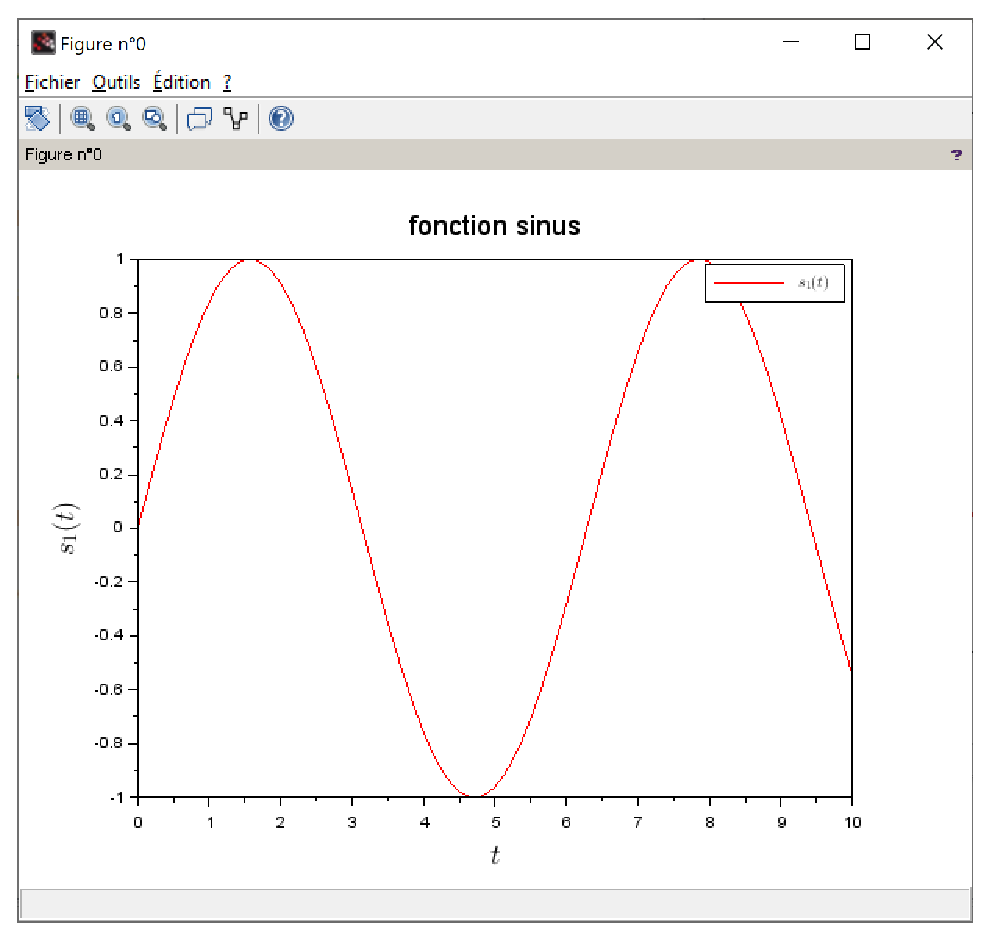
\includegraphics[width=0.8\textwidth]{fig/capture_SCILAB.eps}
    \caption{Capture d'écran de la fenêtre graphique générée par SCILAB.\label{fig-capture-SCILAB}}
\end{figure}

La figure~\cref{fig-capture-SCILAB} présente une capture d'écran 
d'une des fenêtres générées par SCILAB.
          
Les textes des légendes, titre des axes acceptent la syntaxe~\LaTeX.
Il existe de nombreuses commandes pour modifier l'apparence
d'une figure, de ces axes et pour pouvoir la sauvegarder
dans différents formats (vectorielle ou matricielle).
Nous renvoyons au lecteur à la documentation de Scilab pour
cet aspect. Il est également possible d'éditer une image en accédant
au menu de la fenêtre graphique après l'avoir générée.


%%%%%%%%%%%%%%%%%%%%%%%%%%%%%%%%%%%%%%%%%%%%%%%%%%%%%%%%%%%%%%%%%%%%%%%%%%%%%%%%
%%%%%%%%%%%%%%%%%%%%%%%%%%%%%%%%%%%%%%%%%%%%%%%%%%%%%%%%%%%%%%%%%%%%%%%%%%%%%%%%
%%%%%%%%%%%%%%%%%%%%%%%%%%%%%%%%%%%%%%%%%%%%%%%%%%%%%%%%%%%%%%%%%%%%%%%%%%%%%%%%
%%%%%%%%%%%%%%%%%%%%%%%%%%%%%%%%%%%%%%%%%%%%%%%%%%%%%%%%%%%%%%%%%%%%%%%%%%%%%%%%
\section[Programmation]
        {Programmation (source 
        \href{https://fr.wikibooks.org/wiki/Découvrir_Scilab}{Wikibooks}) }
%%%%%%%%%%%%%%%%%%%%%%%%%%%%%%%%%%%%%%%%%%%%%%%%%%%%%%%%%%%%%%%%%%%%%%%%%%%%%%%%
%%%%%%%%%%%%%%%%%%%%%%%%%%%%%%%%%%%%%%%%%%%%%%%%%%%%%%%%%%%%%%%%%%%%%%%%%%%%%%%%
%%%%%%%%%%%%%%%%%%%%%%%%%%%%%%%%%%%%%%%%%%%%%%%%%%%%%%%%%%%%%%%%%%%%%%%%%%%%%%%%
%%%%%%%%%%%%%%%%%%%%%%%%%%%%%%%%%%%%%%%%%%%%%%%%%%%%%%%%%%%%%%%%%%%%%%%%%%%%%%%%

Scilab est également un langage de programmation, il accepte un certain nombre 
d'instructions autres que mathématiques, permettant la formulation et 
l'exécution d'algorithmes : \verb?for, while, if, do, do, case?\ldots ou 
définition de fonction.

L'écriture de programmes se fait idéalement avec l'éditeur de 
texte SciNotes; celui-ci met en exergue les instructions en couleurs, 
les parenthésages (correspondance entre les paires de parenthèses 
et de crochets), et surligne les lignes continuées avec un fond jaune. 
On peut aussi utiliser un autre éditeur de texte en sauvegardant le fichier 
avec l'extension \verb?.sce? ou \verb?.sci?. Lorsque l'environnement le permet,
on peut faire du copier-coller depuis l'éditeur de texte externe vers SciNotes 
ou bien l'éditeur de ligne de commande.

%%%%%%%%%%%%%%%%%%%%%%%%%%%%%%%%%%%%%%%%%%%%%%%%%%%%%%%%%%%%%%%%%%%%%%%%%%%%%%%%
\paragraph{Syntaxe d'une fonction :}
%%%%%%%%%%%%%%%%%%%%%%%%%%%%%%%%%%%%%%%%%%%%%%%%%%%%%%%%%%%%%%%%%%%%%%%%%%%%%%%%

La fonction doit commencer par le mot réservé \verb?function? et finir par 
\verb?endfunction? sous la forme :
\begin{code}
\begin{verbatim}
function [out1,out2,...,outN]=nomfonction(in1,in2,...,inP)

  // out1,out2,...,outN sont les variables de sortie
  // in1,in2,...,inP variables d entree
          
<instructions>
endfunction
\end{verbatim}
\end{code}

Une façon usuelle de définir des fonctions est de mettre 
celles-ci dans un fichier à extension \verb?.sci?. 
Il faut alors la charger avec la fonction \verb?exec()?.
Pour exécuter une fonction, il suffit de l'appeler en passant les 
arguments nécessaires.

%%%%%%%%%%%%%%%%%%%%%%%%%%%%%%%%%%%%%%%%%%%%%%%%%%%%%%%%%%%%%%%%%%%%%%%%%%%%%%%%
\paragraph{Exemple d'une réponse temporelle analytique}
%%%%%%%%%%%%%%%%%%%%%%%%%%%%%%%%%%%%%%%%%%%%%%%%%%%%%%%%%%%%%%%%%%%%%%%%%%%%%%%%
Nous souhaitons tracer la réponse temporelle d'un système linéaire dont la
forme analytique est déterminée et de la forme :
$$
s(t)=\dfrac{1}{2}-e^{-t}-\dfrac{3}{2}e^{-2t}
$$
On écrira la fonction de la façon suivante :
\begin{code}
\begin{verbatim}
function u=s(t)
    u=0.5-exp(-t)+1.5*exp(-2*t)
endfunction
\end{verbatim}
\end{code}

On peut maintenant l'appeler avec un arguments sous la forme de vecteurs. 
\begin{code}
\begin{verbatim}
t=0:0.1:10
plot2d(t,s(t),style=3)
\end{verbatim}
\end{code}
La fonction renvoie un vecteur de même taille que le vecteur \verb?t?.

\begin{center}
    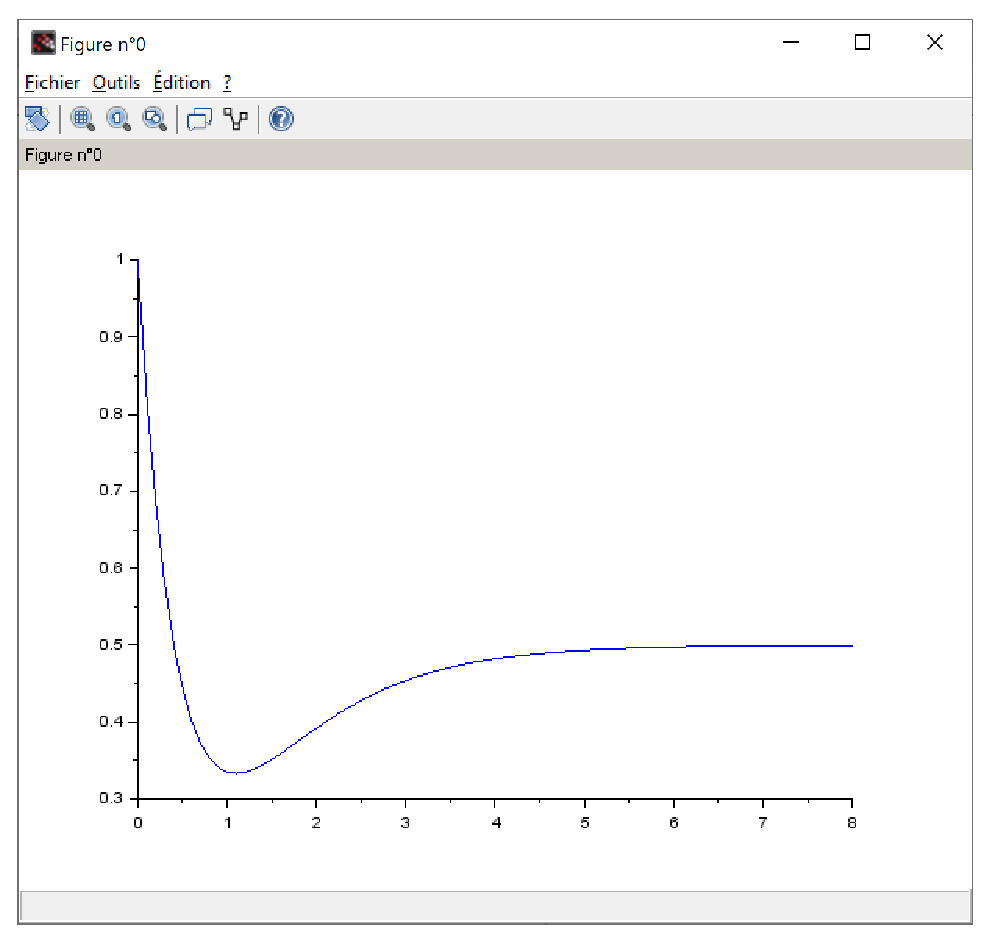
\includegraphics[width=0.5\textwidth]{fig/capture_SCILAB-fonction.eps}
\end{center}

\newpage
%%%%%%%%%%%%%%%%%%%%%%%%%%%%%%%%%%%%%%%%%%%%%%%%%%%%%%%%%%%%%%%%%%%%%%%%%%%%%%%%
%%%%%%%%%%%%%%%%%%%%%%%%%%%%%%%%%%%%%%%%%%%%%%%%%%%%%%%%%%%%%%%%%%%%%%%%%%%%%%%%
%%%%%%%%%%%%%%%%%%%%%%%%%%%%%%%%%%%%%%%%%%%%%%%%%%%%%%%%%%%%%%%%%%%%%%%%%%%%%%%%
\section{\emph{{\scshape SLCI}}~avec Scilab}
%%%%%%%%%%%%%%%%%%%%%%%%%%%%%%%%%%%%%%%%%%%%%%%%%%%%%%%%%%%%%%%%%%%%%%%%%%%%%%%%
%%%%%%%%%%%%%%%%%%%%%%%%%%%%%%%%%%%%%%%%%%%%%%%%%%%%%%%%%%%%%%%%%%%%%%%%%%%%%%%%
%%%%%%%%%%%%%%%%%%%%%%%%%%%%%%%%%%%%%%%%%%%%%%%%%%%%%%%%%%%%%%%%%%%%%%%%%%%%%%%%

Scilab permet de réaliser des études avancées des systèmes linéaires continus 
et invariants.

%%%%%%%%%%%%%%%%%%%%%%%%%%%%%%%%%%%%%%%%%%%%%%%%%%%%%%%%%%%%%%%%%%%%%%%%%%%%%%%%
%%%%%%%%%%%%%%%%%%%%%%%%%%%%%%%%%%%%%%%%%%%%%%%%%%%%%%%%%%%%%%%%%%%%%%%%%%%%%%%%
\subsection{Définition d'un système linéaire}
%%%%%%%%%%%%%%%%%%%%%%%%%%%%%%%%%%%%%%%%%%%%%%%%%%%%%%%%%%%%%%%%%%%%%%%%%%%%%%%%
%%%%%%%%%%%%%%%%%%%%%%%%%%%%%%%%%%%%%%%%%%%%%%%%%%%%%%%%%%%%%%%%%%%%%%%%%%%%%%%%
La définition d'un système linéaire continu se fait avec la fonction 
\verb?syslin?. 

\begin{doc}
%%%%%%%%%%%%%%%%%%%%%%%%%%%%%%%%%%%%%%%%%%%%%%%%%%%%%%%%%%%%%%%%%%%%%%%%%%%%%%%%
\paragraph{Fonction syslin (extrait de la doc officiel: help syslin )}
%%%%%%%%%%%%%%%%%%%%%%%%%%%%%%%%%%%%%%%%%%%%%%%%%%%%%%%%%%%%%%%%%%%%%%%%%%%%%%%%
    \begin{itemize}
        \item Syntaxe :
        \begin{code}
\begin{verbatim}
sl=syslin(dom,N,D)
sl=syslin(dom,H)
\end{verbatim}
        \end{code}
        \item Paramètres :
            \begin{itemize}
                \item \verb?dom? : chaîne de caractères \verb?('c','d')?, 
                      ou \verb?[]? ou un scalaire.
                \item \verb?N,D? : matrices polynomiales
                \item \verb?H?   : matrice rationnelle
                \item \verb?sl?  : tlist (liste de type "\verb?syslin?") 
                      représentant le système dynamique
            \end{itemize}
        \item Description : 
            \begin{itemize}
                \item \verb?syslin? définit un système dynamique linéaire en 
                      tant que liste typée, et vérifie la consistance des 
                      données.
                \item \verb?dom? spécifie le domaine temporel :
                      \verb?dom='c'? pour un système à temps continu, 
                      \verb?dom='d'? pour un système à temps discret, 
                      \verb?n? pour un système échantillonné à la période n 
                      (en secondes), 
                      \verb?dom=[]? si le domaine temporel n'est pas défini
            \end{itemize}
    \end{itemize}
\end{doc}

\paragraph{Exemple d'utilisation}
Pour définir un système linéaire du premier ordre de fonction de transfert
$$
H(p)=\dfrac{K}{1+\tau p}
$$
à l'aide de la fonction \verb?syslin? il existe deux syntaxes, soit en utilisant 
la fraction rationnelle directement \verb?syslin("c",ft)?:
\begin{code}
\begin{verbatim}
// ======================================
//  Définir un système du premier ordre
// ======================================
p=%s                   // indéterminée du polynôme
K=1,tau=1;             // paramètres du système

H=K/(1+tau*p);         // fonction de tranfert

PO=syslin('c',H)       // définition du SLCI PO:PremierOrdre
\end{verbatim}
\end{code}
ou en définisant le numérateur et dénominateur séparément (c.-à-d \verb?syslin("c",num,den)?)
\begin{code}
\begin{verbatim}
p=%s
K=1,tau=1;                // paramètres du système

PO=syslin('c',K,1+tau*p)  // définition du SLCI PO:PremierOrdre
\end{verbatim}
\end{code}

Il faut noter que les paramètres de la fonction de transfert sont affectés de valeurs
numériques. En effet, SCILAB ne peut pas traiter des variables formelles mais uniquement
des variables \og numériques\fg.
%\newpage

%%%%%%%%%%%%%%%%%%%%%%%%%%%%%%%%%%%%%%%%%%%%%%%%%%%%%%%%%%%%%%%%%%%%%%%%%%%%%%%%
%%%%%%%%%%%%%%%%%%%%%%%%%%%%%%%%%%%%%%%%%%%%%%%%%%%%%%%%%%%%%%%%%%%%%%%%%%%%%%%%
\subsection{Simulation temporelle d'un système linéaire}
%%%%%%%%%%%%%%%%%%%%%%%%%%%%%%%%%%%%%%%%%%%%%%%%%%%%%%%%%%%%%%%%%%%%%%%%%%%%%%%%
%%%%%%%%%%%%%%%%%%%%%%%%%%%%%%%%%%%%%%%%%%%%%%%%%%%%%%%%%%%%%%%%%%%%%%%%%%%%%%%%
Pour simuler la réponse temporelle d'un système linéaire on utilisera la fonction 
\verb?csim?.

\begin{doc}
%%%%%%%%%%%%%%%%%%%%%%%%%%%%%%%%%%%%%%%%%%%%%%%%%%%%%%%%%%%%%%%%%%%%%%%%%%%%%%%%
\paragraph{Fonction csim (extrait de la doc officiel (en anglais): help csim )}
%%%%%%%%%%%%%%%%%%%%%%%%%%%%%%%%%%%%%%%%%%%%%%%%%%%%%%%%%%%%%%%%%%%%%%%%%%%%%%%%
\begin{itemize}
    \item Syntax :
    \begin{code}
\begin{verbatim}
[y [,x]]=csim(u,t,sl,[x0 [,tol]])
\end{verbatim}
    \end{code}
    \item Parameters :
    \begin{itemize}
        \item \verb?u?  function, list or string (control)
        \item \verb?t?  real vector specifying times with, \verb?t(1)? is the 
              initial time \verb?(x0=x(t(1)))?.
        \item \verb?sl? syslin list (SIMO linear system) in continuous time.
        \item \verb?y?  a matrix such that \verb?y=[y(t(i)], i=1,..,n?
        \item \verb?x?  a matrix such that \verb?x=[x(t(i)], i=1,..,n?
        \item \verb?tol? a 2 vector \verb?[atol rtol]? defining absolute and 
              relative tolerances for \verb?ode? solver
    \end{itemize}

    \item Description :

    \begin{itemize} 
        \item \verb?csim? simulation of the controlled linear system \verb?sl?.
              \verb?sl? is assumed to be a continuous-time system represented 
              by a \verb?syslin? list.
        \item \verb?u?  is the control and \verb?x0? the initial state.
        \item \verb?y?  is the output and \verb?x? the state.
    \end{itemize}

    The control can be:
    \begin{itemize}
        \item a function : \verb?[inputs]=u(t)?
        \item a list : \verb?list(ut,parameter1,....,parametern)? such that:
              \verb?inputs=ut(t,parameter1,....,parametern)? 
    (\verb?ut? is a function)
        \item the string \verb?"impuls"? for impulse response calculation 
              (here \verb?sl? must have a single input and \verb?x0=0?). 
              For systems with direct feedthrough, the infinite pulse at 
              \verb?t=0? is ignored.
        \item the string \verb?"step"? for step response calculation (here 
              \verb?sl? must have a single input and \verb?x0=0?)
        \item a vector giving the values of \verb?u? corresponding to each 
              \verb?t? value.
\end{itemize}
\end{itemize}
\end{doc}

\paragraph{Exemple d'utilisation}

Pour simuler la réponse impulsionnelle on utilisera la chaîne de caractères 
\verb?'impuls'? (ou les premiers caractères de cette chaîne). 

Il faut également définir le vecteur temps qui imposera la 
taille du vecteur de sortie. Le troisième argument est un système linéaire
définit par la fonction \verb?syslin? présentée précedemment. 
\begin{code}
\begin{verbatim}
t=0.0:0.05:20;              // définition du vecteur 
                            // de temps
// ----------------------
// réponse impulsionnelle
// ----------------------
e1='imp'                    // 'imp' : impulsion de Dirac
s1=csim(e1,t,PO)            // réponse impulsionnelle du sl PO
                            // pour tous les points du vecteur t.

\end{verbatim}
\end{code}
Pour la réponse indicielle, on utilisera la chaîne de caractères \verb?'step'?.
\begin{code}
\begin{verbatim}
t=0.0:0.05:20;              // définition du vecteur 
                            // de temps
// ----------------------
// réponse indicielle 
// ----------------------
e2='step'                   // 'step' : échélon unitaire.
s2=csim(e2,t,PO)            // réponse impulsionnelle du sl PO
                            // pour tous les points du vecteur t.

\end{verbatim}
\end{code}
Pour toute autre fonction, on donnera le vecteur de la fonction explicitement. 
Par exemple pour la réponse à une rampe unitaire on donnera simplement 
le vecteur \verb?t?. \`A noter que pour la réponse indicielle, nous aurions pu utiliser
la fonction \verb?ones? :

\begin{code}
\begin{verbatim}
step=ones(size(t)(1),size(t)(2))
s1=csim(step,t,PO)
\end{verbatim}
\end{code}

On notera que l'on utilise ici la fonction \verb?size()? pour assurer que le vecteur 
de la sollicitation est de même taille que le vecteur \verb?t?. 

\paragraph{Approximation de l'impulsion de Dirac}

Il est possible d'approximée l'impulsion de Dirac par un vecteur dont
les valeurs sont toutes nulles sauf pour sa première composante. 
L'amplitude du \og pic\fg dépendra de l'écart entre deux valeurs du vecteur temps $\Delta t$. 
Les instructions suivantes permettent de verifier cette approximation :

\begin{code}
    \begin{verbatim}
s=%s
//définition d'une fonction de transfert du premier ordre
H=syslin('c',1,1+s+s^2)

t=0:0.001:16
// simulation exacte de la réponse impulsionnelle
exact=csim('imp',t,H)

//approximation de l'impulsion de Dirac
impuls=zeros(size(t)(1),size(t)(2))
impuls(1)=2/(t(2)-t(1))  // "amplitude" de l'impulsion 2/Dt  
//simulation approximée de la réponse impulsionnelle
approx=csim(impuls,t,H)

clf(0)
plot2d(t,[exact' approx'],[1 2])
\end{verbatim}
\end{code}

Cette approximation est d'autant meilleure que l'intervalle $\Delta t$ est petit 
(autrement dit que le nombre de points du vecteur \verb?t?, pour un 
intervalle donnée est grand). On utilisera cette approximation avec prudence.

%%%%%%%%%%%%%%%%%%%%%%%%%%%%%%%%%%%%%%%%%%%%%%%%%%%%%%%%%%%%%%%%%%%%%%%%%%%%%%%%
%%%%%%%%%%%%%%%%%%%%%%%%%%%%%%%%%%%%%%%%%%%%%%%%%%%%%%%%%%%%%%%%%%%%%%%%%%%%%%%%
\subsection{Système du premier ordre}
%%%%%%%%%%%%%%%%%%%%%%%%%%%%%%%%%%%%%%%%%%%%%%%%%%%%%%%%%%%%%%%%%%%%%%%%%%%%%%%%
%%%%%%%%%%%%%%%%%%%%%%%%%%%%%%%%%%%%%%%%%%%%%%%%%%%%%%%%%%%%%%%%%%%%%%%%%%%%%%%%
Soit, un système du premier ordre définit par la fonction de transfert : 
$$
H(p)=\dfrac{K}{1+\tau p }
$$
La définition sous Scilab de ce système se fait simplement par les quelques 
instructions suivantes :
\begin{code}
\begin{verbatim}
// ======================================
//  Définir un système du premier ordre
// ======================================

p=poly(0,'p');
K=1,tau=1;                      // paramètres du système

H=K/(1+tau*p);                  // fonction de tranfert

PremierOrdre=syslin('c',H)      // définition du SLCI
\end{verbatim}
\end{code}

Nous allons maintenant étudier les réponses temporelles 
à différentes excitations du système du premier ordre.
%%%%%%%%%%%%%%%%%%%%%%%%%%%%%%%%%%%%%%%%%%%%%%%%%%%%%%%%%%%%%%%%%%%%%%%%%%%%%%%%
\subsubsection{Réponse impulsionnnelle}
%%%%%%%%%%%%%%%%%%%%%%%%%%%%%%%%%%%%%%%%%%%%%%%%%%%%%%%%%%%%%%%%%%%%%%%%%%%%%%%%
\begin{code}
\begin{verbatim}
// ------------------------
// réponse impulsionnelle
// ------------------------
e2='imp'                        // 'imp' : dirac
s2=csim(e2,t,PremierOrdre);   

scf(1);clf(1);
plot(t,s2,'r')

legend('$s_2(t)$','$e_2(t)$')
xlabel("$t$","fontsize",4);
ylabel("$s(t)$","fontsize",4); 
title('réponse impulsionnelle',"fontsize",4);
\end{verbatim}
\end{code}

%%%%%%%%%%%%%%%%%%%%%%%%%%%%%%%%%%%%%%%%%%%%%%%%%%%%%%%%%%%%%%%%%%%%%%%%%%%%%%%%
\subsubsection{Réponse indicielle}
%%%%%%%%%%%%%%%%%%%%%%%%%%%%%%%%%%%%%%%%%%%%%%%%%%%%%%%%%%%%%%%%%%%%%%%%%%%%%%%%
\begin{code}
\begin{verbatim}

t=0.0:0.05:20;                  // définition du vecteur 
                                // de temps
// ---------------------
//  réponse indicielle
// ---------------------
e1='step'                       // 'step' : échelon
s1=csim(e1,t,PremierOrdre);    

// clf : effacer le contenu de
// la fenêtre graphique
// scf : creer une nouvelle 
// fenêtre graphique

scf(0);clf(0);
plot(t,s1,'r')

legend('$s_1(t)$','$e_1(t)$')
xlabel("$t$","fontsize",4);
ylabel("$s(t)$","fontsize",4); 
title('réponse indicielle',"fontsize",4);
\end{verbatim}
\end{code}


%%%%%%%%%%%%%%%%%%%%%%%%%%%%%%%%%%%%%%%%%%%%%%%%%%%%%%%%%%%%%%%%%%%%%%%%%%%%%%%%
\subsubsection{Réponse à une excitation sinuso\"idale}
%%%%%%%%%%%%%%%%%%%%%%%%%%%%%%%%%%%%%%%%%%%%%%%%%%%%%%%%%%%%%%%%%%%%%%%%%%%%%%%%
\begin{code}
\begin{verbatim}
// -----------------------------------------
// réponse à une excitation sinuso\"idale 
// -----------------------------------------
e3=sin(t)
s3=csim(e3,t,PremierOrdre);

scf(2);clf(2);
plot(t,s3,'r',t,e3,'b')

legend('$s_3(t)$','$e_3(t)$')
xlabel("$t$","fontsize",4);
ylabel("$s(t)$","fontsize",4); 
title('réponse harmonique',"fontsize",4);
\end{verbatim}
\end{code}

Ci-dessous nous présentons une façon d'étudier la réponse temporelle pour
différentes valeurs d'un des paramètres du système du premier ordre.
\begin{code}
\begin{verbatim}
scf(3);clf(3);
for tau=1:1.0:10.
    H2=K/(1+tau*p)
    PremierOrdre=syslin('c',H2)
    e1='step'
    s1=csim(e1,t,PremierOrdre);
    plot(t,s1,'r')
end
\end{verbatim}
\end{code}


%%%%%%%%%%%%%%%%%%%%%%%%%%%%%%%%%%%%%%%%%%%%%%%%%%%%%%%%%%%%%%%%%%%%%%%%%%%%%%%%
\subsubsection{Réponse fréquentielle}
%%%%%%%%%%%%%%%%%%%%%%%%%%%%%%%%%%%%%%%%%%%%%%%%%%%%%%%%%%%%%%%%%%%%%%%%%%%%%%%%
Scilab permet de tracer facilement les différents diagrammes de la réponse 
fréquentielle d'un système. Nous donnons ici les fonctions les 
plus importantes : 
\begin{code}
\begin{verbatim}
fMin =0.01,fMax=100;
p=poly(0,'p')
K=1.,tau=1.;
H=K/(1+tau*p);
PremierOrdre=syslin('c',[K],[1+tau*p])

// diagrammme de Bode
scf(0);clf(0);
bode(PremierOrdre,fMin,fMax); bode_asymp(PremierOrdre,fMin,fMax);

// diagrammme de Nyquist
scf(1);clf(1);
nyquist(PremierOrdre) ;

// diagramme de Black
scf(2);clf(2);
black(PremierOrdre,0.01,10);
nicholschart(colors=color('gray')*[2 2]) //abaque de Black

// Lieu de Evans
scf(3);clf(3);
evans(PremierOrdre) ;
\end{verbatim}
\end{code}

%%%%%%%%%%%%%%%%%%%%%%%%%%%%%%%%%%%%%%%%%%%%%%%%%%%%%%%%%%%%%%%%%%%%%%%%%%%%%%%%
%%%%%%%%%%%%%%%%%%%%%%%%%%%%%%%%%%%%%%%%%%%%%%%%%%%%%%%%%%%%%%%%%%%%%%%%%%%%%%%%
\subsection{Carte des pôles et zéros}
%%%%%%%%%%%%%%%%%%%%%%%%%%%%%%%%%%%%%%%%%%%%%%%%%%%%%%%%%%%%%%%%%%%%%%%%%%%%%%%%
%%%%%%%%%%%%%%%%%%%%%%%%%%%%%%%%%%%%%%%%%%%%%%%%%%%%%%%%%%%%%%%%%%%%%%%%%%%%%%%%
\begin{doc}
%%%%%%%%%%%%%%%%%%%%%%%%%%%%%%%%%%%%%%%%%%%%%%%%%%%%%%%%%%%%%%%%%%%%%%%%%%%%%%%%
\paragraph{Fonction plzr (extrait de la doc officiel (en anglais): help plzr )}
%%%%%%%%%%%%%%%%%%%%%%%%%%%%%%%%%%%%%%%%%%%%%%%%%%%%%%%%%%%%%%%%%%%%%%%%%%%%%%%%
\begin{itemize}
    \item Syntax :
\begin{code}
\begin{verbatim}
plzr(sl)
\end{verbatim}
\end{code}
    \item Arguments :
    \begin{itemize}
        \item \verb?sl? syslin list (SIMO linear system) in continuous time.
    \end{itemize}
    \item Description :
    \begin{itemize}
        \item \verb?plzr(sl)? produces a pole-zero plot of the linear system sl.
    \end{itemize}
\end{itemize}
\end{doc}

\paragraph{Exemple}
Pour tracer la carte des pôles et zéros de la fonction de transfert $H(p)$ définit 
par :
$$
H(p)=\dfrac{p+2}{p^2+p+1}
$$
On utilisera les instructions suivantes:
\begin{code}
\begin{verbatim}
p=%s
H=syslin('c',p+2,p^2+p+1)
plzr(H)
\end{verbatim}
\end{code}

\begin{center}
    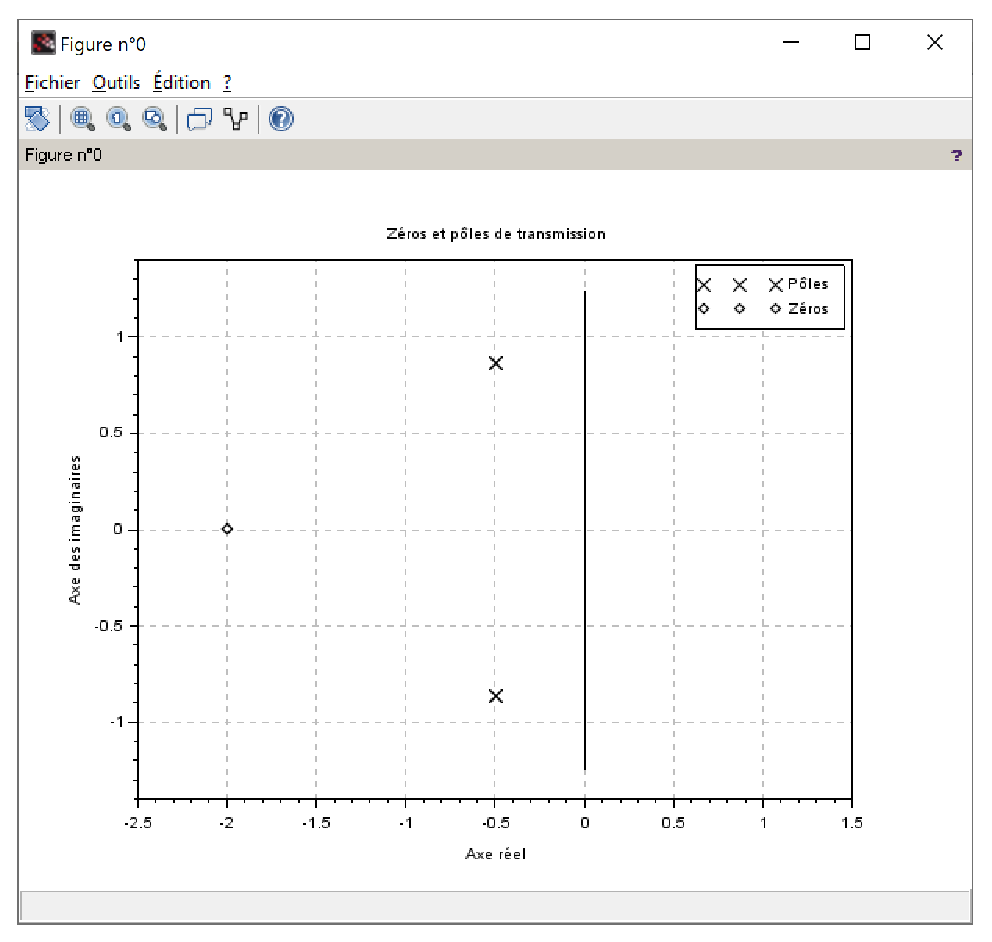
\includegraphics[width=0.8\textwidth]{fig/capture_SCILAB-plzr.eps}
\end{center}
%%%%%%%%%%%%%%%%%%%%%%%%%%%%%%%%%%%%%%%%%%%%%%%%%%%%%%%%%%%%%%%%%%%%%%%%%%%%%%%%
%%%%%%%%%%%%%%%%%%%%%%%%%%%%%%%%%%%%%%%%%%%%%%%%%%%%%%%%%%%%%%%%%%%%%%%%%%%%%%%%
\subsection{Asservissement}
%%%%%%%%%%%%%%%%%%%%%%%%%%%%%%%%%%%%%%%%%%%%%%%%%%%%%%%%%%%%%%%%%%%%%%%%%%%%%%%%
%%%%%%%%%%%%%%%%%%%%%%%%%%%%%%%%%%%%%%%%%%%%%%%%%%%%%%%%%%%%%%%%%%%%%%%%%%%%%%%%
\begin{doc}
%%%%%%%%%%%%%%%%%%%%%%%%%%%%%%%%%%%%%%%%%%%%%%%%%%%%%%%%%%%%%%%%%%%%%%%%%%%%%%%%
\paragraph{Fonction feedback (extrait de la doc officiel (en anglais): 
           help feedback)}
%%%%%%%%%%%%%%%%%%%%%%%%%%%%%%%%%%%%%%%%%%%%%%%%%%%%%%%%%%%%%%%%%%%%%%%%%%%%%%%%
\begin{itemize}
    \item Syntax :
    \begin{code}
\begin{verbatim}
Sl=Sl1/.Sl2
\end{verbatim}
    \end{code}
    \item Parameters :
    \begin{itemize}
        \item \verb?Sl1,Sl2?  linear systems (syslin list) in state-space or 
              transfer form, or ordinary gain matrices.
        \item \verb?Sl? linear system (syslin list) in state-space or 
              transfer form.
    \end{itemize}

    \item Description :

    \begin{itemize} 
        \item The feedback operation is denoted by /. (slashdot). 
        \item This command returns \verb?Sl=Sl1*(I+Sl2*Sl1)^-1?, i.e 
              the (negative) feedback of \verb?Sl1? and \verb?Sl2?. \verb?Sl? 
              is the transfer \verb?v -> y? for 
              \verb?y = Sl1 u?, \verb?u = v - Sl2 y?.
        \item The result is the same as \verb?Sl=LFT([0,I;I,-Sl2],Sl1)?.
        \item Caution: do not use with decimal point (e.g. \verb?1/.1? 
              is ambiguous!)
    \end{itemize}
\end{itemize}
\end{doc}

\paragraph{Exemple}
Imaginons que nous souhaitons déterminer
le système linéaire en boucle fermée à partir des systèmes de la chaîne directe $H(p)$
et la chaîne de retour $R(p)$ comme définit par le schéma-bloc suivant:
\begin{center}
    \tikzsetnextfilename{feedback-annexe_scilab-ext}
    \begin{tikzpicture}
    \bbr
\end{tikzpicture}

\end{center}
Avec cette opération \verb?feedback?, il est possible de déterminer la fonction de transfert 
en boucle fermée en une seule instruction.
\begin{code}
\begin{verbatim}
--> p=%s
--> H=syslin('c',1,1+p);
--> R=syslin('c',1,1+p);
--> HBF=H/.R
 HBF  = 
                 
       1 + s      
     -----------  
               2  
     2 + 2s + s 
\end{verbatim}
\end{code}

%\newpage
%%%%%%%%%%%%%%%%%%%%%%%%%%%%%%%%%%%%%%%%%%%%%%%%%%%%%%%%%%%%%%%%%%%%%%%%%%%%%%%%
%%%%%%%%%%%%%%%%%%%%%%%%%%%%%%%%%%%%%%%%%%%%%%%%%%%%%%%%%%%%%%%%%%%%%%%%%%%%%%%%
%%%%%%%%%%%%%%%%%%%%%%%%%%%%%%%%%%%%%%%%%%%%%%%%%%%%%%%%%%%%%%%%%%%%%%%%%%%%%%%%
\section{Scilab-Xcos}
%%%%%%%%%%%%%%%%%%%%%%%%%%%%%%%%%%%%%%%%%%%%%%%%%%%%%%%%%%%%%%%%%%%%%%%%%%%%%%%%
%%%%%%%%%%%%%%%%%%%%%%%%%%%%%%%%%%%%%%%%%%%%%%%%%%%%%%%%%%%%%%%%%%%%%%%%%%%%%%%%
%%%%%%%%%%%%%%%%%%%%%%%%%%%%%%%%%%%%%%%%%%%%%%%%%%%%%%%%%%%%%%%%%%%%%%%%%%%%%%%%
Nous présentons ici le module Xcos intégré à Scilab. Xcos inclut un 
éditeur graphique pour facilement représenté les schémas fonctionnels
en connectant des blocs entre eux. Cette présentation/tutoriel étant loin 
d'être complète, nous renvoyons le lecteur à la documentation officielle de Xcos
pour obtenir davantage de détails~\cite{steer2014scilab,premier,xcos}. 
%sur l'utilisation de ce module (notamment les références
%suivantes~\cite{steer2014scilab,premier,xcos}, sur lesquelles est basé le 
petit tuto suivant.)

%%%%%%%%%%%%%%%%%%%%%%%%%%%%%%%%%%%%%%%%%%%%%%%%%%%%%%%%%%%%%%%%%%%%%%%%%%%%%%%%
%%%%%%%%%%%%%%%%%%%%%%%%%%%%%%%%%%%%%%%%%%%%%%%%%%%%%%%%%%%%%%%%%%%%%%%%%%%%%%%%
\subsection{Lancer Xcos}
%%%%%%%%%%%%%%%%%%%%%%%%%%%%%%%%%%%%%%%%%%%%%%%%%%%%%%%%%%%%%%%%%%%%%%%%%%%%%%%%
%%%%%%%%%%%%%%%%%%%%%%%%%%%%%%%%%%%%%%%%%%%%%%%%%%%%%%%%%%%%%%%%%%%%%%%%%%%%%%%%
Après avoir lancé Scilab, éxécuter une des instructions suivantes :
\begin{itemize}
    \item Taper la commande \verb?xcos? dans la console;
    \item Cliquer sur l'icône : \raisebox{-\mydepth}{\fbox{
          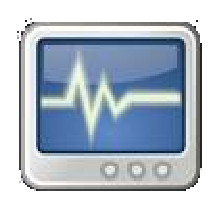
\includegraphics[height=\myheight]{fig/xcos.eps}}}
    \item Menu $\rightarrow$ Applications $\rightarrow$ Xcos
\end{itemize}

Xcos ouvre par défaut le navigateur de palettes et une fenêtre d'édition. 
Pour construire le diagramme il suffit de faire glisser les blocs dans la 
fenêtre d'édition.

%%%%%%%%%%%%%%%%%%%%%%%%%%%%%%%%%%%%%%%%%%%%%%%%%%%%%%%%%%%%%%%%%%%%%%%%%%%%%%%%
%%%%%%%%%%%%%%%%%%%%%%%%%%%%%%%%%%%%%%%%%%%%%%%%%%%%%%%%%%%%%%%%%%%%%%%%%%%%%%%%
\subsection{Diagramme simple}
%%%%%%%%%%%%%%%%%%%%%%%%%%%%%%%%%%%%%%%%%%%%%%%%%%%%%%%%%%%%%%%%%%%%%%%%%%%%%%%%
%%%%%%%%%%%%%%%%%%%%%%%%%%%%%%%%%%%%%%%%%%%%%%%%%%%%%%%%%%%%%%%%%%%%%%%%%%%%%%%%

Le module inclut un grand nombre de blocs (c.f Navigateur de palettes).
Il est possible de construire des super-blocs qui incorpore d'autres blocs pour
faciliter la lecture d'un diagramme complexe. \newline
Nous allons créer un diagramme simple. Pour celà, placer les blocs suivants 
dans la fenêtre d'édition:

\begin{table}[!h]
    \centering
    \begin{tabular}{@{}P{4cm}P{6cm}P{4cm}@{}}
    \toprule
    Désignation   & Représentation & Sous-palette \\
    \midrule
    \'Echelon     & 
    \begin{minipage}{6cm}
    \centering
    
\includegraphics[width=0.25\linewidth]{fig/scilab05.eps}
    \end{minipage} &
    Sources / STEP\_FUNCTION \\
    \midrule
    Fonction de transfert continue     & 
    \begin{minipage}{6cm}
    \centering
    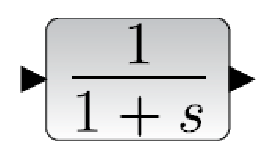
\includegraphics[width=0.25\linewidth]{fig/scilab06.eps}
    \end{minipage} & 
    Systèmes à temps continu / CLR \\
    \midrule
    Horloge       & 
    \begin{minipage}{6cm}
    \centering
    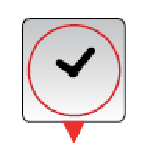
\includegraphics[width=0.2\linewidth]{fig/scilab07.eps}
    \end{minipage} & 
    Sources / Clock\_c \\
    \midrule
    Visualisation & 
    \begin{minipage}{6cm}
    \centering
    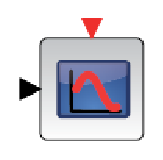
\includegraphics[width=0.25\linewidth]{fig/scilab08.eps}
    \end{minipage} & 
    Sinks / CSCOPE \\
    \bottomrule
\end{tabular}
\end{table}

Connecter les blocs pour obtenir le schéma bloc Xcos de la 
figure~\ref{fig-simple}.

\begin{figure}
    \centering
    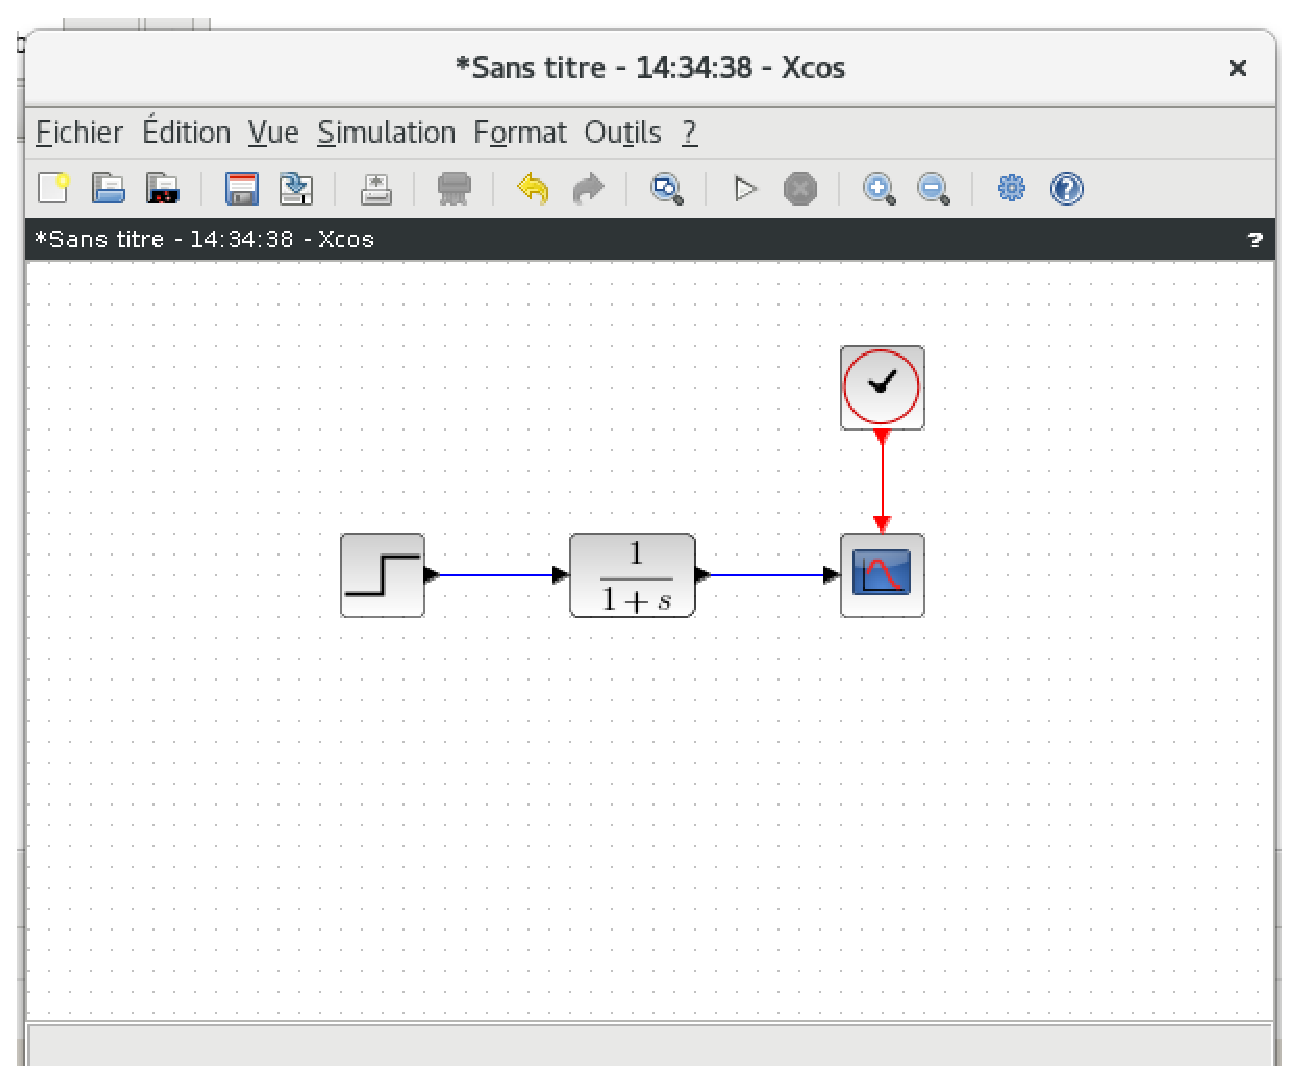
\includegraphics[width=0.5\textwidth]{fig/diagramme_simple.eps}
    \caption{Exemple de diagramme simple\label{fig-simple}}
\end{figure}

Il faut maintenant simuler et visualiser les résultats.  

%\newpage
%%%%%%%%%%%%%%%%%%%%%%%%%%%%%%%%%%%%%%%%%%%%%%%%%%%%%%%%%%%%%%%%%%%%%%%%%%%%%%%%
%%%%%%%%%%%%%%%%%%%%%%%%%%%%%%%%%%%%%%%%%%%%%%%%%%%%%%%%%%%%%%%%%%%%%%%%%%%%%%%%
\subsection{Simulation}
%%%%%%%%%%%%%%%%%%%%%%%%%%%%%%%%%%%%%%%%%%%%%%%%%%%%%%%%%%%%%%%%%%%%%%%%%%%%%%%%
%%%%%%%%%%%%%%%%%%%%%%%%%%%%%%%%%%%%%%%%%%%%%%%%%%%%%%%%%%%%%%%%%%%%%%%%%%%%%%%%
Pour lancer une simulation : cliquer sur l'icône : 
\raisebox{-\mydepth}{
    \fbox{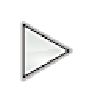
\includegraphics[height=\myheight]{fig/demarrage.eps}}
}

Pour arrêter une simulation : cliquer sur l'icône : 
\raisebox{-\mydepth}{
    \fbox{
\includegraphics[height=\myheight]{fig/stop.eps}}
}

Plusieurs paramètres peuvent être ajustés :
\begin{itemize}
    \item La durée de la simulation : Simulation $\rightarrow$ 
          Configurer $\rightarrow$ Temps d'intégration final
    \item La période d'échantillonage : Cliquer sur l'horloge.
    \item La fonction échelon  : Cliquer sur le bloc de la fonction échelon
    \item Les paramètres de la fonction de transfert : Cliquer sur le bloc CLR 
          (N'oubliez pas d'ajouter un contexte si vous utiliser des variables)
\end{itemize}

%%%%%%%%%%%%%%%%%%%%%%%%%%%%%%%%%%%%%%%%%%%%%%%%%%%%%%%%%%%%%%%%%%%%%%%%%%%%%%%%
%%%%%%%%%%%%%%%%%%%%%%%%%%%%%%%%%%%%%%%%%%%%%%%%%%%%%%%%%%%%%%%%%%%%%%%%%%%%%%%%
\subsection{Blocs \og To Workspace \fg~ou \og From Workspace\fg}
%%%%%%%%%%%%%%%%%%%%%%%%%%%%%%%%%%%%%%%%%%%%%%%%%%%%%%%%%%%%%%%%%%%%%%%%%%%%%%%%
%%%%%%%%%%%%%%%%%%%%%%%%%%%%%%%%%%%%%%%%%%%%%%%%%%%%%%%%%%%%%%%%%%%%%%%%%%%%%%%%
On utilisera les blocs particuliers dans le cas où l'on souhaite 
utiliser des données à partir de Scilab (\og From Workspace\fg) 
ou récupérer ces données après la simulation (\og To Workspace \fg).

\begin{figure}[!h]
    \centering
    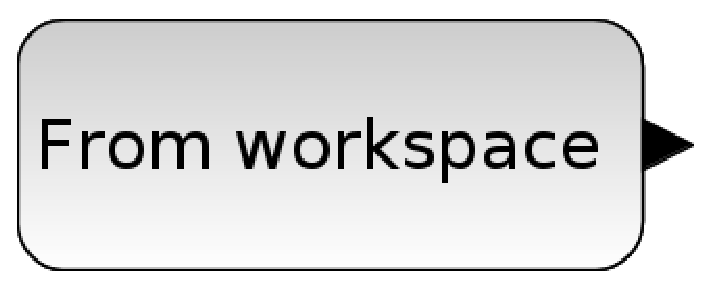
\includegraphics[width=0.25\textwidth]{fig/FROMWSB.eps}\hspace{3cm}
    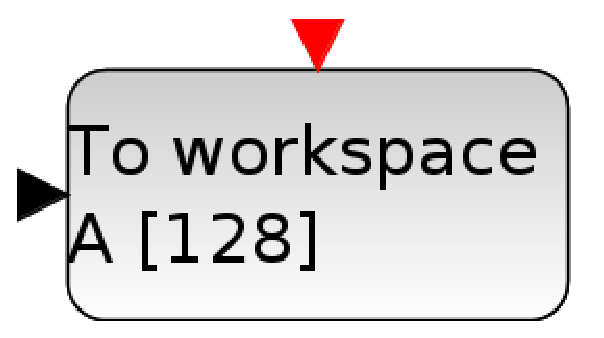
\includegraphics[width=0.25\textwidth]{fig/TOWS_c.eps}
    \caption{Blocs d'échange avec Scilab\label{fig-workspace}}
\end{figure}
%%%%%%%%%%%%%%%%%%%%%%%%%%%%%%%%%%%%%%%%%%%%%%%%%%%%%%%%%%%%%%%%%%%%%%%%%%%%%%%%
%%%%%%%%%%%%%%%%%%%%%%%%%%%%%%%%%%%%%%%%%%%%%%%%%%%%%%%%%%%%%%%%%%%%%%%%%%%%%%%%
%%%%%%%%%%%%%%%%%%%%%%%%%%%%%%%%%%%%%%%%%%%%%%%%%%%%%%%%%%%%%%%%%%%%%%%%%%%%%%%%
%%%%%%%%%%%%%%%%%%%%%%%%%%%%%%%%%%%%%%%%%%%%%%%%%%%%%%%%%%%%%%%%%%%%%%%%%%%%%%%%
%annexe_scilab.tex
           %I Scilab
}
%%%%%%%%%%%%%%%%%%%%%%%%%%%%%%%%%%%%%%%%%%%%%%%%%%%%%%%%%%%%%%%%%%%%%%%%%%%%%%%%
%%%%%%%%%%%%%%%%%%%%%%%%%%%%%%%%%%%%%%%%%%%%%%%%%%%%%%%%%%%%%%%%%%%%%%%%%%%%%%%%
%%%%%%%%%%%%%%%%%%%%%%%%%%%%%%%%%%%%%%%%%%%%%%%%%%%%%%%%%%%%%%%%%%%%%%%%%%%%%%%%
%%%%%%%%%%%%%%%%%%%%%%%%%%%%%%%%%%%%%%%%%%%%%%%%%%%%%%%%%%%%%%%%%%%%%%%%%%%%%%%%
\chapter{\'Echelle logarithmique et le décibel~\label{annexe-log}}
%%%%%%%%%%%%%%%%%%%%%%%%%%%%%%%%%%%%%%%%%%%%%%%%%%%%%%%%%%%%%%%%%%%%%%%%%%%%%%%%
%%%%%%%%%%%%%%%%%%%%%%%%%%%%%%%%%%%%%%%%%%%%%%%%%%%%%%%%%%%%%%%%%%%%%%%%%%%%%%%%
%%%%%%%%%%%%%%%%%%%%%%%%%%%%%%%%%%%%%%%%%%%%%%%%%%%%%%%%%%%%%%%%%%%%%%%%%%%%%%%%
%%%%%%%%%%%%%%%%%%%%%%%%%%%%%%%%%%%%%%%%%%%%%%%%%%%%%%%%%%%%%%%%%%%%%%%%%%%%%%%%

En automatique, l'échelle logarithmique est très fréquement 
utilisée pour permettre la représentation
graphique de variables dont les valeurs s'étalent sur plusieurs ordres 
de grandeur. Pour les diagrammes de Bode, il est courant de représenter le gain 
d'un \gls{slci}~en décibel \textbf{dB} qui est également une unité liée au 
logarithme décimale. La maitrise du calcul logarithmique est donc indispensable
pour l'établissement d'un diagramme de Bode.

%%%%%%%%%%%%%%%%%%%%%%%%%%%%%%%%%%%%%%%%%%%%%%%%%%%%%%%%%%%%%%%%%%%%%%%%%%%%%%%%
%%%%%%%%%%%%%%%%%%%%%%%%%%%%%%%%%%%%%%%%%%%%%%%%%%%%%%%%%%%%%%%%%%%%%%%%%%%%%%%%
%%%%%%%%%%%%%%%%%%%%%%%%%%%%%%%%%%%%%%%%%%%%%%%%%%%%%%%%%%%%%%%%%%%%%%%%%%%%%%%%
\section{Rappel sur le logarithme décimal}
%%%%%%%%%%%%%%%%%%%%%%%%%%%%%%%%%%%%%%%%%%%%%%%%%%%%%%%%%%%%%%%%%%%%%%%%%%%%%%%%
%%%%%%%%%%%%%%%%%%%%%%%%%%%%%%%%%%%%%%%%%%%%%%%%%%%%%%%%%%%%%%%%%%%%%%%%%%%%%%%%
%%%%%%%%%%%%%%%%%%%%%%%%%%%%%%%%%%%%%%%%%%%%%%%%%%%%%%%%%%%%%%%%%%%%%%%%%%%%%%%%
Le logarithme décimal (noté $\log$ ou $\log_{10}$) est le logarithme en base 10.
La propriété principale du logarithme est de transformer un produit en 
somme\footnote{C'est pour cette propriété qu'il fut introduit par John Napier 
en 1614 pour faciliter les calculs de produit quelconque en établissant une 
correspondance avec la somme de logarithme à l'aide de tables de logarithme, 
ceci avant le développement de calculateur numérique performant.}.

Formellement, la fonction logarithme décimal $\log{(x)}$ est défini 
analytiquement par 
$$
\log{(x)}=\dfrac{\ln{(x)}}{\ln{(10)}}
$$
où la fonction $\ln{x}$ est la fonction logarithme néperien (i.e en base 
naturelle $e$) 

%%%%%%%%%%%%%%%%%%%%%%%%%%%%%%%%%%%%%%%%%%%%%%%%%%%%%%%%%%%%%%%%%%%%%%%%%%%%%%%%
\paragraph{Propriétés}
%%%%%%%%%%%%%%%%%%%%%%%%%%%%%%%%%%%%%%%%%%%%%%%%%%%%%%%%%%%%%%%%%%%%%%%%%%%%%%%%
\begin{itemize}
    \item $\log{(ab)}=\log{(a)} + \log{(b)}$
    \item $\log{\left(\dfrac{a}{b}\right)}=\log{a} - \log{(b)}$
    \item $\log{(a^n)}=n\log{(a)}$
    \item $\log{\sqrt[n]{(a)}}=\dfrac{1}{n}\log{(a)}$
    \item $\log(x)=a \Leftrightarrow x=10^a $; $\log(1) = 0$; 
          $\log(10) = 1$ ; $\log(0.1) = -1$
\end{itemize}


%%%%%%%%%%%%%%%%%%%%%%%%%%%%%%%%%%%%%%%%%%%%%%%%%%%%%%%%%%%%%%%%%%%%%%%%%%%%%%%%
%%%%%%%%%%%%%%%%%%%%%%%%%%%%%%%%%%%%%%%%%%%%%%%%%%%%%%%%%%%%%%%%%%%%%%%%%%%%%%%%
%%%%%%%%%%%%%%%%%%%%%%%%%%%%%%%%%%%%%%%%%%%%%%%%%%%%%%%%%%%%%%%%%%%%%%%%%%%%%%%%
\section{\'Echelle logarithmique décimale}
%%%%%%%%%%%%%%%%%%%%%%%%%%%%%%%%%%%%%%%%%%%%%%%%%%%%%%%%%%%%%%%%%%%%%%%%%%%%%%%%
%%%%%%%%%%%%%%%%%%%%%%%%%%%%%%%%%%%%%%%%%%%%%%%%%%%%%%%%%%%%%%%%%%%%%%%%%%%%%%%%
%%%%%%%%%%%%%%%%%%%%%%%%%%%%%%%%%%%%%%%%%%%%%%%%%%%%%%%%%%%%%%%%%%%%%%%%%%%%%%%%
Sur une \textbf{échelle linéaire} décimale classique, des couples de 
graduations dont la \textbf{différence} ($\Delta$ ci-dessous) vaut 10 sont à 
égales distances. 

\begin{center}
\tikzsetnextfilename{log_1-annexeJ-ext}
\begin{tikzpicture}
    \draw[-latex] (0,0) -- (11,0) ;
    \foreach \x in {0,...,20}
         \draw (\x/2,2pt) -- (\x/2,-2pt);
    \foreach \x in {0,10,20} 
    {
        \draw (\x/2,4pt) -- (\x/2,-4pt);
        \node [below,yshift=-0.5em] at (\x/2,2pt) {\small \x};
    }
    \foreach \x in {4,14}
    \node [above,yshift=0.0em] at (\x/2,2pt) {\small \x};
    \draw[blue,thick] (0,0.2) -- (0,1.2) ;
    \draw[blue,thick] (5,0.2) -- (5,1.2) ;
    \draw[blue,thick] (10,0.2) -- (10,1.2) ;
    \draw[utb,latex-latex] (0,0.75) -- node[above] {$\Delta=10$} (5,0.75);
    \draw[utb,latex-latex] (5,0.75) -- node[above] {$\Delta=10$} (10,0.75);
    \draw[red,thick] (2,-0.2) -- (2,-1.22) ;
    \draw[red,thick] (7,-0.2) -- (7,-1.2) ;
    \draw[utr,latex-latex] (2,-0.75) -- node[below] {$\Delta=10$} (7,-0.75);
\end{tikzpicture}
\end{center}

Sur une \textbf{échelle logarithmique} décimale, des couples de graduations 
dont le \textbf{rapport} ($\alpha$ ci-dessous) vaut 10 sont à égales distances.

\begin{center}
\tikzsetnextfilename{log_2-annexeJ-ext}
\begin{tikzpicture}
    \draw[-latex] (0,0) -- (11,0) ;
    \foreach \x in {1.0,10.0,100.0} {
        \coordinate (P1) at ({5*log10(\x)},4pt);
        \coordinate (P2) at ({5*log10(\x)},-4pt);
        \draw[] (P1) -- (P2);
    }
    \foreach \x in {2.0,3.0,4.0,5.0,6.0,7.0,8.0,9.0,
                    20.0,30.0,40.0,50.0,60.0,70.0,80.0,90.0} 
    {
        \coordinate (P1) at ({5*log10(\x)},2pt);
        \coordinate (P2) at ({5*log10(\x)},-2pt);
        \draw[] (P1) -- (P2);
    }
    \foreach \x in {1,10,100}
         \node [below,yshift=-0.5em] at ({5*log10(\x)},2pt) {\small \x};
    \foreach \x in {3,30}
         \node [above,yshift=0.0em] at ({5*log10(\x)},2pt) {\small \x};
    \draw[blue,thick] (0,0.2) -- (0,1.2) ;
    \draw[blue,thick] (5,0.2) -- (5,1.2) ;
    \draw[blue,thick] (10,0.2) -- (10,1.2) ;
    \draw[utb,latex-latex] (0,0.75) -- node[above] {$\alpha=10$} (5,0.75);
    \draw[utb,latex-latex] (5,0.75) -- node[above] {$\alpha=10$} (10,0.75);
    \draw[red,thick] (2.386,-0.2) -- (2.386,-1.2) ;
    \draw[red,thick] (7.386,-0.2) -- (7.386,-1.2) ;
    \draw[red,ultra thick,latex-latex] (2.386,-0.75) -- 
    node[below] {$\alpha=10$} (7.386,-0.75);
\end{tikzpicture}
\end{center}

On généralise cette l'égalité entre le rapport et n'importe quelle 
distance constante sur l'axe à échelle logarithmique.

\begin{center}
\tikzsetnextfilename{log_3-annexeJ-ext}
\begin{tikzpicture}
    \draw[-latex] (0,0) -- (11,0) ;
    \foreach \x in {2.0,3.0,4.0,5.0,6.0,7.0,8.0,9.0,
                    20.0,30.0,40.0,50.0,60.0,70.0,80.0,90.0} 
    {
        \coordinate (P1) at ({5*log10(\x)},2pt);
        \coordinate (P2) at ({5*log10(\x)},-2pt);
        \draw[] (P1) -- (P2);
    }
    \foreach \x in {1.0,10.0,100.0} {
        \coordinate (P1) at ({5*log10(\x)},4pt);
        \coordinate (P2) at ({5*log10(\x)},-4pt);
        \draw[] (P1) -- (P2);
    }
    \foreach \x in {1,10,100}
         \node [below,yshift=-0.5em] at ({5*log10(\x)},2pt) {\small \x};
    \foreach \x in {1,2,4,8,16,32,64}
         \node [above,yshift=0em,blue] at ({5*log10(\x)},1.3) {\small \x};
    \foreach \x in {1,2,4,8,16,32,64} 
    {
    \pgfmathsetmacro{\lx}{5*log10(\x)}
    \pgfmathsetmacro{\lnx}{5*log10(\x*2)}
    \ifthenelse{\equal{\x}{64}}
    {\draw[blue,thick] (\lx,0.2) -- (\lx,1.2);}
    {\draw[blue,thick] (\lx,0.2) -- (\lx,1.2);
    \draw[utb,latex-latex] (\lx,0.75) -- node[above] {$\alpha=2$} (\lnx,0.75);}
    }
\end{tikzpicture}
\end{center}
On remarquera que dans le cas ci-dessus, les valeurs 16,32 et 64 n'ont pas 
de graduation qui leurs sont propres mais ces valeurs sont bien déterminées 
par la distance constante entre deux graduation de rapport $\alpha=2$. 

Il existe une terminologie pour se référer à des rapport $\alpha$ particuliers,
on parle d'\textbf{octave}\footnote{Pour le lecteur mélomane, celà correspond à
la définition de l'octave musicale. Par exemple, l'octave supérieur du 
La (noté La4) de fréquence \SI{440}{\hertz} est de fréquence égale à 
\SI{880}{\hertz} (noté La3).} lorsque $\alpha=2$ et de \textbf{décade} 
lorsque $\alpha=10$

Avec cette terminologie, une atténuation du gain d'une réponse harmonique de 
\SI{-20}{\dB} lorsque la pulsation augmente d'un facteur 10, se dira 
\SI{-20}{\dB\per\dec} ou \SI{-6}{\dB\per\oct}.

\newpage
%%%%%%%%%%%%%%%%%%%%%%%%%%%%%%%%%%%%%%%%%%%%%%%%%%%%%%%%%%%%%%%%%%%%%%%%%%%%%%%%
%%%%%%%%%%%%%%%%%%%%%%%%%%%%%%%%%%%%%%%%%%%%%%%%%%%%%%%%%%%%%%%%%%%%%%%%%%%%%%%%
%%%%%%%%%%%%%%%%%%%%%%%%%%%%%%%%%%%%%%%%%%%%%%%%%%%%%%%%%%%%%%%%%%%%%%%%%%%%%%%%
\section{Le décibel}
%%%%%%%%%%%%%%%%%%%%%%%%%%%%%%%%%%%%%%%%%%%%%%%%%%%%%%%%%%%%%%%%%%%%%%%%%%%%%%%%
%%%%%%%%%%%%%%%%%%%%%%%%%%%%%%%%%%%%%%%%%%%%%%%%%%%%%%%%%%%%%%%%%%%%%%%%%%%%%%%%
%%%%%%%%%%%%%%%%%%%%%%%%%%%%%%%%%%%%%%%%%%%%%%%%%%%%%%%%%%%%%%%%%%%%%%%%%%%%%%%%
Le bel (B) est une unité de grandeur sans dimension 
exprimant la valeur relative entre deux quantités (de puissances en 
particuliers) par le logarithme décimal de leur rapport. Le décibel (\si{\dB}), 
plus couramment utilisé, est définie comme un dixieme de bel, et donc 
correspond à dix fois le logarithme décimal du rapport.
$$
X_{dB}=10\log{\dfrac{P_s}{P_e}}
$$

Le gain en décibel reporté sur un diagramme de Bode correspond à 
la valeur relative à 1 du carré du gain $G$ (le carré de l'amplitude d'un 
signal pouvant être définit comme une puissance). Ainsi,
$$
G_{dB}=10\log{G^2} = 20\log{G}
$$
Nous rappellons que le gain $G(\omega)$, dit naturel, est le module de la
fonction de transfert $G(\omega)=|H(\jw)|$. Le~\cref{tab-equiv_dB} donne 
l'équivalence entre le gain naturel $G$ et gain décibel $G_{dB}$ pour 
différentes valeurs particulières frequemment rencontrées dans ce cours.

\begin{table}[!t]
    \begin{tabular}{@{}P{1cm}P{1cm}P{1cm}P{1cm}P{1cm}
                       P{1cm}P{1cm}P{1cm}P{1cm}P{1cm}@{}}
    \toprule
    $G$      & 0.01&0.1&0.5     &$\sqrt{2}/2$&1&$\sqrt{2}$&2       &10&100   \\
    \midrule
    $G_{dB}$ & -40 &-20&$\sim$-6&$\sim$-3    &0&$\sim$3   &$\sim$6 & 20 & 40 \\
    \bottomrule
    \end{tabular}
    \caption{\'Equivalence entre gain naturel $G$ et gain 
             décibel $G_{dB}$. D'après~\cite{laroche}\label{tab-equiv_dB}}
\end{table}


%%%%%%%%%%%%%%%%%%%%%%%%%%%%%%%%%%%%%%%%%%%%%%%%%%%%%%%%%%%%%%%%%%%%%%%%%%%%%%%%
%%%%%%%%%%%%%%%%%%%%%%%%%%%%%%%%%%%%%%%%%%%%%%%%%%%%%%%%%%%%%%%%%%%%%%%%%%%%%%%%
%%%%%%%%%%%%%%%%%%%%%%%%%%%%%%%%%%%%%%%%%%%%%%%%%%%%%%%%%%%%%%%%%%%%%%%%%%%%%%%%
\section{Diagramme de Bode}
%%%%%%%%%%%%%%%%%%%%%%%%%%%%%%%%%%%%%%%%%%%%%%%%%%%%%%%%%%%%%%%%%%%%%%%%%%%%%%%%
%%%%%%%%%%%%%%%%%%%%%%%%%%%%%%%%%%%%%%%%%%%%%%%%%%%%%%%%%%%%%%%%%%%%%%%%%%%%%%%%
%%%%%%%%%%%%%%%%%%%%%%%%%%%%%%%%%%%%%%%%%%%%%%%%%%%%%%%%%%%%%%%%%%%%%%%%%%%%%%%%

Un diagramme de Bode d'un fonction complexe $H(\jw)$ est composé de deux 
courbes (i.e gain et phase) en représentation semi-logarithmique.

Soit la fonction complexe du premier ordre telle que 
\begin{align}
H(\jw)=\dfrac{1}{1+\jw}\label{eq-ft_annexe}
\end{align}

%%%%%%%%%%%%%%%%%%%%%%%%%%%%%%%%%%%%%%%%%%%%%%%%%%%%%%%%%%%%%%%%%%%%%%%%%%%%%%%%
\paragraph{Tracé du gain}
%%%%%%%%%%%%%%%%%%%%%%%%%%%%%%%%%%%%%%%%%%%%%%%%%%%%%%%%%%%%%%%%%%%%%%%%%%%%%%%%
Le gain de cette fonction de transfert $G(\omega)=|H(\jw)|$ s'écrit :
$$
G(\omega)=\dfrac{1}{\sqrt{1+\omega^2}}
$$
le gain en décibel est donc :
$$
G_{dB}(\omega)=20\log{\dfrac{1}{\sqrt{1+\omega^2}}}=-20\log{\sqrt{1+\omega^2}}
$$
C'est cette fonction qu'il faut tracer point par point sur le diagramme 
de Bode, cependant il est généralement recommandé d'étudier les asymptotes 
de cette fonction avant de tracer la courbe. Pour les basses fréquences, le 
gain en décibel ce commporte comme 
$$
G_{dB}(\omega)\sim-20\log{1}\sim 0\text{dB}
$$ 
et pour les hautes fréquences, comme
$$
G_{dB}(\omega)\sim -20\log{\omega}.
$$
Dans le cas des hautes fréquences, lorsque la pulsation est mutiplié par 
10 (i.e une décade ) le gain diminue de \SI{-20}{\dB}, on dit également 
qu'à haute fréquence le gain possède une pente de \textbf{-20dB par décade}. 
La pulsation de coupure est ici de $\omega_{c}=1$, c'est cette pulsation qui 
marque la \og séparation\fg entre basses et hautes fréquences. 

\begin{figure}[!t]
\centering
\tikzsetnextfilename{bode_1-annexeJ-ext}
\begin{tikzpicture}
\begin{axis}
    [   ticklabel style = {font=\footnotesize},
        width=0.9\textwidth,
        height=0.22\textheight,
        ylabel={Gain (dB)},
        xtick={1e-3,1e-2,1e-1,1,1e1,1e2,1e3}, 
        ytick={-60,-50,-40,-30,-20,-10,0,10}, 
        xticklabels={\tp[-3],\tp,\tp,\tp,\tp,\tp,\tp},
        yticklabels={-60,-50,-40,-30,-20,-10,0,10},
        xmode=log,ymode=normal,
        xmin=1e-3, xmax=1e3,
        ymin=-60, ymax=10,
        grid=both,
        major grid style={black!40}
    ]
    \addplot[signalb,domain=1e-3:1e3]        {-20*log10(sqrt(1+x*x))}; 
    \addplot[signalr,dashed,domain=1e-3:1e0] {0};
    \addplot[signalr,dashed,domain=1e0:1e3]  {-20*log10(x)};
\end{axis}
\end{tikzpicture}
\tikzsetnextfilename{bode_2-annexeJ-ext}
\begin{tikzpicture}
    \begin{axis}
    [   ticklabel style = {font=\footnotesize},
        width=0.9\textwidth,
        height=0.22\textheight,
        xlabel={Pulsation (rad/s)},
        ylabel={Phase (\degree)},
        xtick={1e-3,1e-2,1e-1,1,1e1,1e2,1e3}, 
        ytick={-90,-45,0}, 
        yticklabels={-90,-45,0},
        xticklabels={\tp[-3],\tp,\tp,\tp,\tp,\tp,\tp},
        xmode=log,ymode=normal,
        xmin=1e-3, xmax=1e3,
            ymin=-90, ymax=0,
        grid=both,
        major grid style={black!40}
    ]
    \addplot[signalb,domain=1e-3:1e3] {-atan(x)}; 
    \addplot[signalr,dashed,domain=1e-3:1e0] {0};
    \addplot[signalr,dashed,domain=1e0:1e3]  {-90};
    \draw[signalr,dashed] (axis cs:1,0) -- (axis cs:1,-90);
\end{axis}
\end{tikzpicture}
    \caption{Diagramme de Bode d'un système du premier ordre.
    \label{fig-bode_annexe}}
\end{figure}

%%%%%%%%%%%%%%%%%%%%%%%%%%%%%%%%%%%%%%%%%%%%%%%%%%%%%%%%%%%%%%%%%%%%%%%%%%%%%%%%
\paragraph{Tracé de la phase}
%%%%%%%%%%%%%%%%%%%%%%%%%%%%%%%%%%%%%%%%%%%%%%%%%%%%%%%%%%%%%%%%%%%%%%%%%%%%%%%%
La phase $\phi(\omega)$ correspond à l'argument principale (\Cref{annexe-NC}) 
de la fonction complexe $H(\jw)$.
$$
\phi(\omega)=\arg{H(\jw)}=-\arg{(1+\jw)}=-\arctan{\omega}
$$
C'est cette fonction $\phi(\omega)$ qu'il faut tracer point par point 
sur le diagramme de Bode, mais comme précedemment
il est conseillé de déterminer les asymptotes à basse et haute fréquence.
\`A basse fréquence, la phase se comporte comme,
$$
\phi(\omega)\sim 0
$$ 
et à haute fréquence, comme, 
$$
\phi(\omega)\sim -\dfrac{\pi}{2}.
$$
Les asymptotes sont une approximation bien plus 
grossière dans le cas de la phase. 
En générale, il est recommandé de 
calculer la phase pour des valeurs particulières de la 
pulsation. Par exemple, à la pulsation de coupure, 
lorsque $\omega=$1, la phase est de -45\degree, en effet,
$$
\phi(1)=-\arg{(1+\jw)}=-\dfrac{\pi}{4}
$$

La~\cref{fig-bode_annexe} présente le diagramme de Bode associé à 
la fonction de transfert de l'\cref{eq-ft_annexe}.

\newpage
%%%%%%%%%%%%%%%%%%%%%%%%%%%%%%%%%%%%%%%%%%%%%%%%%%%%%%%%%%%%%%%%%%%%%%%%%%%%%%%%
%%%%%%%%%%%%%%%%%%%%%%%%%%%%%%%%%%%%%%%%%%%%%%%%%%%%%%%%%%%%%%%%%%%%%%%%%%%%%%%%
%%%%%%%%%%%%%%%%%%%%%%%%%%%%%%%%%%%%%%%%%%%%%%%%%%%%%%%%%%%%%%%%%%%%%%%%%%%%%%%%
\section{Tracé d'un diagramme de Bode avec Scilab}
%%%%%%%%%%%%%%%%%%%%%%%%%%%%%%%%%%%%%%%%%%%%%%%%%%%%%%%%%%%%%%%%%%%%%%%%%%%%%%%%
%%%%%%%%%%%%%%%%%%%%%%%%%%%%%%%%%%%%%%%%%%%%%%%%%%%%%%%%%%%%%%%%%%%%%%%%%%%%%%%%
%%%%%%%%%%%%%%%%%%%%%%%%%%%%%%%%%%%%%%%%%%%%%%%%%%%%%%%%%%%%%%%%%%%%%%%%%%%%%%%%
Deux fonctions permettent de tracer un diagramme de Bode avec Scilab.
\begin{itemize}
    \item \verb?bode(syslin,fMin,fMax)? trace le diagramme de Bode réel. 
          Cette fonction prend pour argument \verb?sys? un système linéaire 
          comme défini à l'~\Cref{annexe-scilab}, \verb?fMin? et \verb?fMax? 
          une fréquence minimal et maximal (en \si{\hertz} sauf si un 
          4ème argument est donné). 
    \item \verb?bode_asymp(syslin,fMin,fMax)? trace le diagramme asymptotique.
\end{itemize}


\begin{code}
\begin{verbatim}
// ============================================================
//                   Analyse Fréquentielle
// ============================================================
scf(grf);clf(grf);grf=grf+1;
fMin =0.01,fMax=100;
p=poly(0,'p')
PremierOrdre=syslin('c',[1],[1+p])
//-----------------------------------
// diagrammme de Bode
//-----------------------------------
bode(PremierOrdre,fMin,fMax,"rad");
// ----------------------------------
// diagrammme de Bode asymptotique
//-----------------------------------
bode_asymp(PremierOrdre,fMin,fMax);
\end{verbatim}
\end{code}
%%%%%%%%%%%%%%%%%%%%%%%%%%%%%%%%%%%%%%%%%%%%%%%%%%%%%%%%%%%%%%%%%%%%%%%%%%%%%%%%
%%%%%%%%%%%%%%%%%%%%%%%%%%%%%%%%%%%%%%%%%%%%%%%%%%%%%%%%%%%%%%%%%%%%%%%%%%%%%%%%
%%%%%%%%%%%%%%%%%%%%%%%%%%%%%%%%%%%%%%%%%%%%%%%%%%%%%%%%%%%%%%%%%%%%%%%%%%%%%%%%
%%%%%%%%%%%%%%%%%%%%%%%%%%%%%%%%%%%%%%%%%%%%%%%%%%%%%%%%%%%%%%%%%%%%%%%%%%%%%%%%
%annexe_log.tex
               %J Echelle log  
%%%%%%%%%%%%%%%%%%%%%%%%%%%%%%%%%%%%%%%%%%%%%%%%%%%%%%%%%%%%%%%%%%%%%%%%%%%%%%%
\chapter{Transformée de Laplace inverse~\label{annexe-invL}}
%%%%%%%%%%%%%%%%%%%%%%%%%%%%%%%%%%%%%%%%%%%%%%%%%%%%%%%%%%%%%%%%%%%%%%%%%%%%%%%

\section{Contexte}

Il existe une forme analytique de la transformée inverse basée sur                                                            
la formule de Mellin-Fourier\cite{Ostertag}:                                                                                  
$$                                                                                                                            
s(t)=\laplacei{S(p)}=\int_{c-j\infty}^{c+j\infty} e^{pt}S(p)\dd{p}                                                            
$$    

\section{Méthode de Gaver-Stehfest}

\section{Méthode de Talbot fixe}
              %L Laplace inverse 
%%%%%%%%%%%%%%%%%%%%%%%%%%%%%%%%%%%%%%%%%%%%%%%%%%%%%%%%%%%%%%%%%%%%%%%%%%%%%%%%%
%%%%%%%%%%%%%%%%%%%%%%%%%%%%%%%%%%%%%%%%%%%%%%%%%%%%%%%%%%%%%%%%%%%%%%%%%%%%%%%%
%%%%%%%%%%%%%%%%%%%%%%%%%%%%%%%%%%%%%%%%%%%%%%%%%%%%%%%%%%%%%%%%%%%%%%%%%%%%%%%%
%%%%%%%%%%%%%%%%%%%%%%%%%%%%%%%%%%%%%%%%%%%%%%%%%%%%%%%%%%%%%%%%%%%%%%%%%%%%%%%%
\chapter{TODO}
%%%%%%%%%%%%%%%%%%%%%%%%%%%%%%%%%%%%%%%%%%%%%%%%%%%%%%%%%%%%%%%%%%%%%%%%%%%%%%%%
%%%%%%%%%%%%%%%%%%%%%%%%%%%%%%%%%%%%%%%%%%%%%%%%%%%%%%%%%%%%%%%%%%%%%%%%%%%%%%%%
%%%%%%%%%%%%%%%%%%%%%%%%%%%%%%%%%%%%%%%%%%%%%%%%%%%%%%%%%%%%%%%%%%%%%%%%%%%%%%%%
%%%%%%%%%%%%%%%%%%%%%%%%%%%%%%%%%%%%%%%%%%%%%%%%%%%%%%%%%%%%%%%%%%%%%%%%%%%%%%%%
%%%%%%%%%%%%%%%%%%%%%%%%%%%%%%%%%%%%%%%%%%%%%%%%%%%%%%%%%%%%%%%%%%%%%%%%%%%%%%%%
%%%%%%%%%%%%%%%%%%%%%%%%%%%%%%%%%%%%%%%%%%%%%%%%%%%%%%%%%%%%%%%%%%%%%%%%%%%%%%%%
%%%%%%%%%%%%%%%%%%%%%%%%%%%%%%%%%%%%%%%%%%%%%%%%%%%%%%%%%%%%%%%%%%%%%%%%%%%%%%%%
\section*{Figures à retravailler}
%%%%%%%%%%%%%%%%%%%%%%%%%%%%%%%%%%%%%%%%%%%%%%%%%%%%%%%%%%%%%%%%%%%%%%%%%%%%%%%%
%%%%%%%%%%%%%%%%%%%%%%%%%%%%%%%%%%%%%%%%%%%%%%%%%%%%%%%%%%%%%%%%%%%%%%%%%%%%%%%%
%%%%%%%%%%%%%%%%%%%%%%%%%%%%%%%%%%%%%%%%%%%%%%%%%%%%%%%%%%%%%%%%%%%%%%%%%%%%%%%%
%-------------------------------------------------------------------------------
\begin{itemize}
    \item \verb?1er_imp-chap2_ext? : revoir la dimension de la figure
    \item \verb?2nd_pp-chap2_ext? : tracer pour $K=1$ et $E_0=1$
    \item \verb?bode_1er_6-chap_ext? : revoir l'intervalle des pulsations
    \item \verb?carte-chap0_ext? : utiliser le package poles
    \item \verb?integrateur_1-chap2_ext? : à revoir totalement (dimensions)
    \item \verb?pole_dominant-chap0_ext? : dimensions
    \item \verb?sb_fleche-chap1_ext? : les flêches semblent coupés, linewidth
    \item \verb?sb_point-chap1_ext?: linewidth
    \item \verb?sol_eq_diff-chap0-ext? : dimensions + grilles à retravailler
\end{itemize}
%-------------------------------------------------------------------------------
%%%%%%%%%%%%%%%%%%%%%%%%%%%%%%%%%%%%%%%%%%%%%%%%%%%%%%%%%%%%%%%%%%%%%%%%%%%%%%%%
%%%%%%%%%%%%%%%%%%%%%%%%%%%%%%%%%%%%%%%%%%%%%%%%%%%%%%%%%%%%%%%%%%%%%%%%%%%%%%%%
%%%%%%%%%%%%%%%%%%%%%%%%%%%%%%%%%%%%%%%%%%%%%%%%%%%%%%%%%%%%%%%%%%%%%%%%%%%%%%%%
\section*{Pour tous les chapitres}
%%%%%%%%%%%%%%%%%%%%%%%%%%%%%%%%%%%%%%%%%%%%%%%%%%%%%%%%%%%%%%%%%%%%%%%%%%%%%%%%
%%%%%%%%%%%%%%%%%%%%%%%%%%%%%%%%%%%%%%%%%%%%%%%%%%%%%%%%%%%%%%%%%%%%%%%%%%%%%%%%
%%%%%%%%%%%%%%%%%%%%%%%%%%%%%%%%%%%%%%%%%%%%%%%%%%%%%%%%%%%%%%%%%%%%%%%%%%%%%%%%
%-------------------------------------------------------------------------------
\begin{itemize}
\item Donner un identifiant pour chacune des figures tikz pour que la 
      compilation soit plus rapide
\item Ponctuation des équations en relation avec leur place dans le texte.
\item Regrouper les infos suivantes dans une annexe dédiée, pour chaque 
      réponse temporelle du 1er et du 2nd ordre:
%-------------------------------------------------------------------------------
    \begin{itemize}
        \item valeur initiale (pente à l'origine)
        \item valeur finale (pente à l'infinie)
        \item forme analytique des réponses
    \end{itemize}
%-------------------------------------------------------------------------------
\item Unité de $\tau$
\item \'Etablir le transitoire de la réponse harmonique du 1er ordre et/ou 
      2nd ordre.
\item Rappeler que le théorème de la valeur finale ne s'applique que si le 
      système est stable asymptotiquement
\end{itemize}
%-------------------------------------------------------------------------------
%%%%%%%%%%%%%%%%%%%%%%%%%%%%%%%%%%%%%%%%%%%%%%%%%%%%%%%%%%%%%%%%%%%%%%%%%%%%%%%%
%%%%%%%%%%%%%%%%%%%%%%%%%%%%%%%%%%%%%%%%%%%%%%%%%%%%%%%%%%%%%%%%%%%%%%%%%%%%%%%%
%%%%%%%%%%%%%%%%%%%%%%%%%%%%%%%%%%%%%%%%%%%%%%%%%%%%%%%%%%%%%%%%%%%%%%%%%%%%%%%%
\section*{\Cref{avant-propos}}     
%%%%%%%%%%%%%%%%%%%%%%%%%%%%%%%%%%%%%%%%%%%%%%%%%%%%%%%%%%%%%%%%%%%%%%%%%%%%%%%%
%%%%%%%%%%%%%%%%%%%%%%%%%%%%%%%%%%%%%%%%%%%%%%%%%%%%%%%%%%%%%%%%%%%%%%%%%%%%%%%%
%%%%%%%%%%%%%%%%%%%%%%%%%%%%%%%%%%%%%%%%%%%%%%%%%%%%%%%%%%%%%%%%%%%%%%%%%%%%%%%%
%%%%%%%%%%%%%%%%%%%%%%%%%%%%%%%%%%%%%%%%%%%%%%%%%%%%%%%%%%%%%%%%%%%%%%%%%%%%%%%%
%%%%%%%%%%%%%%%%%%%%%%%%%%%%%%%%%%%%%%%%%%%%%%%%%%%%%%%%%%%%%%%%%%%%%%%%%%%%%%%%
%%%%%%%%%%%%%%%%%%%%%%%%%%%%%%%%%%%%%%%%%%%%%%%%%%%%%%%%%%%%%%%%%%%%%%%%%%%%%%%%
\section*{\Cref{chap-slci}}     
%%%%%%%%%%%%%%%%%%%%%%%%%%%%%%%%%%%%%%%%%%%%%%%%%%%%%%%%%%%%%%%%%%%%%%%%%%%%%%%%
%%%%%%%%%%%%%%%%%%%%%%%%%%%%%%%%%%%%%%%%%%%%%%%%%%%%%%%%%%%%%%%%%%%%%%%%%%%%%%%%
%%%%%%%%%%%%%%%%%%%%%%%%%%%%%%%%%%%%%%%%%%%%%%%%%%%%%%%%%%%%%%%%%%%%%%%%%%%%%%%%
%-------------------------------------------------------------------------------
\begin{itemize}
\item Notion de retard à présenter avant la présentation des signaux usuels
\item Régime transitoire/permanent avant l'introduction de la TL
\item Définition de l'équation différentielle à coefficients constants avant 
      l'introduction de la TL
\item Cas de CI non nulles (Réponse forcée/libre)
\end{itemize}
%-------------------------------------------------------------------------------
%%%%%%%%%%%%%%%%%%%%%%%%%%%%%%%%%%%%%%%%%%%%%%%%%%%%%%%%%%%%%%%%%%%%%%%%%%%%%%%%
%%%%%%%%%%%%%%%%%%%%%%%%%%%%%%%%%%%%%%%%%%%%%%%%%%%%%%%%%%%%%%%%%%%%%%%%%%%%%%%%
%%%%%%%%%%%%%%%%%%%%%%%%%%%%%%%%%%%%%%%%%%%%%%%%%%%%%%%%%%%%%%%%%%%%%%%%%%%%%%%%
\section*{\Cref{chap-schemabloc}}
%%%%%%%%%%%%%%%%%%%%%%%%%%%%%%%%%%%%%%%%%%%%%%%%%%%%%%%%%%%%%%%%%%%%%%%%%%%%%%%%
%%%%%%%%%%%%%%%%%%%%%%%%%%%%%%%%%%%%%%%%%%%%%%%%%%%%%%%%%%%%%%%%%%%%%%%%%%%%%%%%
%%%%%%%%%%%%%%%%%%%%%%%%%%%%%%%%%%%%%%%%%%%%%%%%%%%%%%%%%%%%%%%%%%%%%%%%%%%%%%%%

%%%%%%%%%%%%%%%%%%%%%%%%%%%%%%%%%%%%%%%%%%%%%%%%%%%%%%%%%%%%%%%%%%%%%%%%%%%%%%%%
%%%%%%%%%%%%%%%%%%%%%%%%%%%%%%%%%%%%%%%%%%%%%%%%%%%%%%%%%%%%%%%%%%%%%%%%%%%%%%%%
%%%%%%%%%%%%%%%%%%%%%%%%%%%%%%%%%%%%%%%%%%%%%%%%%%%%%%%%%%%%%%%%%%%%%%%%%%%%%%%%
\section*{\Cref{chap-model}}
%%%%%%%%%%%%%%%%%%%%%%%%%%%%%%%%%%%%%%%%%%%%%%%%%%%%%%%%%%%%%%%%%%%%%%%%%%%%%%%%
%%%%%%%%%%%%%%%%%%%%%%%%%%%%%%%%%%%%%%%%%%%%%%%%%%%%%%%%%%%%%%%%%%%%%%%%%%%%%%%%
%%%%%%%%%%%%%%%%%%%%%%%%%%%%%%%%%%%%%%%%%%%%%%%%%%%%%%%%%%%%%%%%%%%%%%%%%%%%%%%%
Ecrire les valeurs finales pour le second ordre.
%%%%%%%%%%%%%%%%%%%%%%%%%%%%%%%%%%%%%%%%%%%%%%%%%%%%%%%%%%%%%%%%%%%%%%%%%%%%%%%%
%%%%%%%%%%%%%%%%%%%%%%%%%%%%%%%%%%%%%%%%%%%%%%%%%%%%%%%%%%%%%%%%%%%%%%%%%%%%%%%%
%%%%%%%%%%%%%%%%%%%%%%%%%%%%%%%%%%%%%%%%%%%%%%%%%%%%%%%%%%%%%%%%%%%%%%%%%%%%%%%%
\section*{\Cref{chap-repfreq}}
%%%%%%%%%%%%%%%%%%%%%%%%%%%%%%%%%%%%%%%%%%%%%%%%%%%%%%%%%%%%%%%%%%%%%%%%%%%%%%%%
%%%%%%%%%%%%%%%%%%%%%%%%%%%%%%%%%%%%%%%%%%%%%%%%%%%%%%%%%%%%%%%%%%%%%%%%%%%%%%%%
%%%%%%%%%%%%%%%%%%%%%%%%%%%%%%%%%%%%%%%%%%%%%%%%%%%%%%%%%%%%%%%%%%%%%%%%%%%%%%%%
%-------------------------------------------------------------------------------
\begin{itemize}
    \item (fait) \'Etablir le transitoire de la réponse 
          harmonique du 1er ordre et/ou 2nd ordre.
\item Distinguer clairement les 3 régimes dans le cas de la réponse harmonique:
%-------------------------------------------------------------------------------
    \begin{itemize}
        \item Apériodique       $\Rightarrow$ 2 systèmes du 1er ordre
        \item Critique          $\Rightarrow$ rien de spécial
        \item Pseudo-périodique $\Rightarrow$ phénomène de résonance
    \end{itemize}
%-------------------------------------------------------------------------------
\end{itemize}
%-------------------------------------------------------------------------------
%%%%%%%%%%%%%%%%%%%%%%%%%%%%%%%%%%%%%%%%%%%%%%%%%%%%%%%%%%%%%%%%%%%%%%%%%%%%%%%%
%%%%%%%%%%%%%%%%%%%%%%%%%%%%%%%%%%%%%%%%%%%%%%%%%%%%%%%%%%%%%%%%%%%%%%%%%%%%%%%%
%%%%%%%%%%%%%%%%%%%%%%%%%%%%%%%%%%%%%%%%%%%%%%%%%%%%%%%%%%%%%%%%%%%%%%%%%%%%%%%%
\section*{\Cref{chap-asservis}}
%%%%%%%%%%%%%%%%%%%%%%%%%%%%%%%%%%%%%%%%%%%%%%%%%%%%%%%%%%%%%%%%%%%%%%%%%%%%%%%%
%%%%%%%%%%%%%%%%%%%%%%%%%%%%%%%%%%%%%%%%%%%%%%%%%%%%%%%%%%%%%%%%%%%%%%%%%%%%%%%%
%%%%%%%%%%%%%%%%%%%%%%%%%%%%%%%%%%%%%%%%%%%%%%%%%%%%%%%%%%%%%%%%%%%%%%%%%%%%%%%%
%-------------------------------------------------------------------------------
\begin{itemize}
    \item FTCD, FTBO à introduire dans le cas de l'asservissement
    \item Place les définitions des temps de réponse, montée avant la 
          modélisation, ou alors définition locale et traiter le problème 
          d'abord le chapitre des performances et caractéristiques d'un 
          système asservi.
\end{itemize}
%-------------------------------------------------------------------------------
%%%%%%%%%%%%%%%%%%%%%%%%%%%%%%%%%%%%%%%%%%%%%%%%%%%%%%%%%%%%%%%%%%%%%%%%%%%%%%%%
%%%%%%%%%%%%%%%%%%%%%%%%%%%%%%%%%%%%%%%%%%%%%%%%%%%%%%%%%%%%%%%%%%%%%%%%%%%%%%%%
%%%%%%%%%%%%%%%%%%%%%%%%%%%%%%%%%%%%%%%%%%%%%%%%%%%%%%%%%%%%%%%%%%%%%%%%%%%%%%%%
\section*{\Cref{chap-perf}}
%%%%%%%%%%%%%%%%%%%%%%%%%%%%%%%%%%%%%%%%%%%%%%%%%%%%%%%%%%%%%%%%%%%%%%%%%%%%%%%%
%%%%%%%%%%%%%%%%%%%%%%%%%%%%%%%%%%%%%%%%%%%%%%%%%%%%%%%%%%%%%%%%%%%%%%%%%%%%%%%%
%%%%%%%%%%%%%%%%%%%%%%%%%%%%%%%%%%%%%%%%%%%%%%%%%%%%%%%%%%%%%%%%%%%%%%%%%%%%%%%%

%%%%%%%%%%%%%%%%%%%%%%%%%%%%%%%%%%%%%%%%%%%%%%%%%%%%%%%%%%%%%%%%%%%%%%%%%%%%%%%%
%%%%%%%%%%%%%%%%%%%%%%%%%%%%%%%%%%%%%%%%%%%%%%%%%%%%%%%%%%%%%%%%%%%%%%%%%%%%%%%%
%%%%%%%%%%%%%%%%%%%%%%%%%%%%%%%%%%%%%%%%%%%%%%%%%%%%%%%%%%%%%%%%%%%%%%%%%%%%%%%%
\section*{\Cref{chap-stab}}
%%%%%%%%%%%%%%%%%%%%%%%%%%%%%%%%%%%%%%%%%%%%%%%%%%%%%%%%%%%%%%%%%%%%%%%%%%%%%%%%
%%%%%%%%%%%%%%%%%%%%%%%%%%%%%%%%%%%%%%%%%%%%%%%%%%%%%%%%%%%%%%%%%%%%%%%%%%%%%%%%
%%%%%%%%%%%%%%%%%%%%%%%%%%%%%%%%%%%%%%%%%%%%%%%%%%%%%%%%%%%%%%%%%%%%%%%%%%%%%%%%

%%%%%%%%%%%%%%%%%%%%%%%%%%%%%%%%%%%%%%%%%%%%%%%%%%%%%%%%%%%%%%%%%%%%%%%%%%%%%%%%
%%%%%%%%%%%%%%%%%%%%%%%%%%%%%%%%%%%%%%%%%%%%%%%%%%%%%%%%%%%%%%%%%%%%%%%%%%%%%%%%
%%%%%%%%%%%%%%%%%%%%%%%%%%%%%%%%%%%%%%%%%%%%%%%%%%%%%%%%%%%%%%%%%%%%%%%%%%%%%%%%
\section*{\Cref{chap-correc}}
%%%%%%%%%%%%%%%%%%%%%%%%%%%%%%%%%%%%%%%%%%%%%%%%%%%%%%%%%%%%%%%%%%%%%%%%%%%%%%%%
%%%%%%%%%%%%%%%%%%%%%%%%%%%%%%%%%%%%%%%%%%%%%%%%%%%%%%%%%%%%%%%%%%%%%%%%%%%%%%%%
%%%%%%%%%%%%%%%%%%%%%%%%%%%%%%%%%%%%%%%%%%%%%%%%%%%%%%%%%%%%%%%%%%%%%%%%%%%%%%%%

%%%%%%%%%%%%%%%%%%%%%%%%%%%%%%%%%%%%%%%%%%%%%%%%%%%%%%%%%%%%%%%%%%%%%%%%%%%%%%%%
%%%%%%%%%%%%%%%%%%%%%%%%%%%%%%%%%%%%%%%%%%%%%%%%%%%%%%%%%%%%%%%%%%%%%%%%%%%%%%%%
%%%%%%%%%%%%%%%%%%%%%%%%%%%%%%%%%%%%%%%%%%%%%%%%%%%%%%%%%%%%%%%%%%%%%%%%%%%%%%%%
\section*{\Cref{chap-repreEtat}}
%%%%%%%%%%%%%%%%%%%%%%%%%%%%%%%%%%%%%%%%%%%%%%%%%%%%%%%%%%%%%%%%%%%%%%%%%%%%%%%%
%%%%%%%%%%%%%%%%%%%%%%%%%%%%%%%%%%%%%%%%%%%%%%%%%%%%%%%%%%%%%%%%%%%%%%%%%%%%%%%%
%%%%%%%%%%%%%%%%%%%%%%%%%%%%%%%%%%%%%%%%%%%%%%%%%%%%%%%%%%%%%%%%%%%%%%%%%%%%%%%%

%%%%%%%%%%%%%%%%%%%%%%%%%%%%%%%%%%%%%%%%%%%%%%%%%%%%%%%%%%%%%%%%%%%%%%%%%%%%%%%%
%%%%%%%%%%%%%%%%%%%%%%%%%%%%%%%%%%%%%%%%%%%%%%%%%%%%%%%%%%%%%%%%%%%%%%%%%%%%%%%%
%%%%%%%%%%%%%%%%%%%%%%%%%%%%%%%%%%%%%%%%%%%%%%%%%%%%%%%%%%%%%%%%%%%%%%%%%%%%%%%%
\section*{\Cref{annexe-lap}}
%%%%%%%%%%%%%%%%%%%%%%%%%%%%%%%%%%%%%%%%%%%%%%%%%%%%%%%%%%%%%%%%%%%%%%%%%%%%%%%%
%%%%%%%%%%%%%%%%%%%%%%%%%%%%%%%%%%%%%%%%%%%%%%%%%%%%%%%%%%%%%%%%%%%%%%%%%%%%%%%%
%%%%%%%%%%%%%%%%%%%%%%%%%%%%%%%%%%%%%%%%%%%%%%%%%%%%%%%%%%%%%%%%%%%%%%%%%%%%%%%%

%%%%%%%%%%%%%%%%%%%%%%%%%%%%%%%%%%%%%%%%%%%%%%%%%%%%%%%%%%%%%%%%%%%%%%%%%%%%%%%%
%%%%%%%%%%%%%%%%%%%%%%%%%%%%%%%%%%%%%%%%%%%%%%%%%%%%%%%%%%%%%%%%%%%%%%%%%%%%%%%%
%%%%%%%%%%%%%%%%%%%%%%%%%%%%%%%%%%%%%%%%%%%%%%%%%%%%%%%%%%%%%%%%%%%%%%%%%%%%%%%%
\section*{\Cref{annexe-NC}}
%%%%%%%%%%%%%%%%%%%%%%%%%%%%%%%%%%%%%%%%%%%%%%%%%%%%%%%%%%%%%%%%%%%%%%%%%%%%%%%%
%%%%%%%%%%%%%%%%%%%%%%%%%%%%%%%%%%%%%%%%%%%%%%%%%%%%%%%%%%%%%%%%%%%%%%%%%%%%%%%%
%%%%%%%%%%%%%%%%%%%%%%%%%%%%%%%%%%%%%%%%%%%%%%%%%%%%%%%%%%%%%%%%%%%%%%%%%%%%%%%%

%%%%%%%%%%%%%%%%%%%%%%%%%%%%%%%%%%%%%%%%%%%%%%%%%%%%%%%%%%%%%%%%%%%%%%%%%%%%%%%%
%%%%%%%%%%%%%%%%%%%%%%%%%%%%%%%%%%%%%%%%%%%%%%%%%%%%%%%%%%%%%%%%%%%%%%%%%%%%%%%%
%%%%%%%%%%%%%%%%%%%%%%%%%%%%%%%%%%%%%%%%%%%%%%%%%%%%%%%%%%%%%%%%%%%%%%%%%%%%%%%%
\section*{\Cref{annexe-DES}}
%%%%%%%%%%%%%%%%%%%%%%%%%%%%%%%%%%%%%%%%%%%%%%%%%%%%%%%%%%%%%%%%%%%%%%%%%%%%%%%%
%%%%%%%%%%%%%%%%%%%%%%%%%%%%%%%%%%%%%%%%%%%%%%%%%%%%%%%%%%%%%%%%%%%%%%%%%%%%%%%%
%%%%%%%%%%%%%%%%%%%%%%%%%%%%%%%%%%%%%%%%%%%%%%%%%%%%%%%%%%%%%%%%%%%%%%%%%%%%%%%%

%%%%%%%%%%%%%%%%%%%%%%%%%%%%%%%%%%%%%%%%%%%%%%%%%%%%%%%%%%%%%%%%%%%%%%%%%%%%%%%%
%%%%%%%%%%%%%%%%%%%%%%%%%%%%%%%%%%%%%%%%%%%%%%%%%%%%%%%%%%%%%%%%%%%%%%%%%%%%%%%%
%%%%%%%%%%%%%%%%%%%%%%%%%%%%%%%%%%%%%%%%%%%%%%%%%%%%%%%%%%%%%%%%%%%%%%%%%%%%%%%%
\section*{\Cref{annexe-2nd}}
%%%%%%%%%%%%%%%%%%%%%%%%%%%%%%%%%%%%%%%%%%%%%%%%%%%%%%%%%%%%%%%%%%%%%%%%%%%%%%%%
%%%%%%%%%%%%%%%%%%%%%%%%%%%%%%%%%%%%%%%%%%%%%%%%%%%%%%%%%%%%%%%%%%%%%%%%%%%%%%%%
%%%%%%%%%%%%%%%%%%%%%%%%%%%%%%%%%%%%%%%%%%%%%%%%%%%%%%%%%%%%%%%%%%%%%%%%%%%%%%%%

%%%%%%%%%%%%%%%%%%%%%%%%%%%%%%%%%%%%%%%%%%%%%%%%%%%%%%%%%%%%%%%%%%%%%%%%%%%%%%%%
%%%%%%%%%%%%%%%%%%%%%%%%%%%%%%%%%%%%%%%%%%%%%%%%%%%%%%%%%%%%%%%%%%%%%%%%%%%%%%%%
%%%%%%%%%%%%%%%%%%%%%%%%%%%%%%%%%%%%%%%%%%%%%%%%%%%%%%%%%%%%%%%%%%%%%%%%%%%%%%%%
\section*{\Cref{annexe-scilab}}
%%%%%%%%%%%%%%%%%%%%%%%%%%%%%%%%%%%%%%%%%%%%%%%%%%%%%%%%%%%%%%%%%%%%%%%%%%%%%%%%
%%%%%%%%%%%%%%%%%%%%%%%%%%%%%%%%%%%%%%%%%%%%%%%%%%%%%%%%%%%%%%%%%%%%%%%%%%%%%%%%
%%%%%%%%%%%%%%%%%%%%%%%%%%%%%%%%%%%%%%%%%%%%%%%%%%%%%%%%%%%%%%%%%%%%%%%%%%%%%%%%

%%%%%%%%%%%%%%%%%%%%%%%%%%%%%%%%%%%%%%%%%%%%%%%%%%%%%%%%%%%%%%%%%%%%%%%%%%%%%%%%
%%%%%%%%%%%%%%%%%%%%%%%%%%%%%%%%%%%%%%%%%%%%%%%%%%%%%%%%%%%%%%%%%%%%%%%%%%%%%%%%
%%%%%%%%%%%%%%%%%%%%%%%%%%%%%%%%%%%%%%%%%%%%%%%%%%%%%%%%%%%%%%%%%%%%%%%%%%%%%%%%
\section*{\Cref{annexe-log}}
%%%%%%%%%%%%%%%%%%%%%%%%%%%%%%%%%%%%%%%%%%%%%%%%%%%%%%%%%%%%%%%%%%%%%%%%%%%%%%%%
%%%%%%%%%%%%%%%%%%%%%%%%%%%%%%%%%%%%%%%%%%%%%%%%%%%%%%%%%%%%%%%%%%%%%%%%%%%%%%%%
%%%%%%%%%%%%%%%%%%%%%%%%%%%%%%%%%%%%%%%%%%%%%%%%%%%%%%%%%%%%%%%%%%%%%%%%%%%%%%%%

%%%%%%%%%%%%%%%%%%%%%%%%%%%%%%%%%%%%%%%%%%%%%%%%%%%%%%%%%%%%%%%%%%%%%%%%%%%%%%%%
%%%%%%%%%%%%%%%%%%%%%%%%%%%%%%%%%%%%%%%%%%%%%%%%%%%%%%%%%%%%%%%%%%%%%%%%%%%%%%%%
%%%%%%%%%%%%%%%%%%%%%%%%%%%%%%%%%%%%%%%%%%%%%%%%%%%%%%%%%%%%%%%%%%%%%%%%%%%%%%%%
\section*{Idée d'après 6.003 MIT}
%%%%%%%%%%%%%%%%%%%%%%%%%%%%%%%%%%%%%%%%%%%%%%%%%%%%%%%%%%%%%%%%%%%%%%%%%%%%%%%%
%%%%%%%%%%%%%%%%%%%%%%%%%%%%%%%%%%%%%%%%%%%%%%%%%%%%%%%%%%%%%%%%%%%%%%%%%%%%%%%%
%%%%%%%%%%%%%%%%%%%%%%%%%%%%%%%%%%%%%%%%%%%%%%%%%%%%%%%%%%%%%%%%%%%%%%%%%%%%%%%%
%-------------------------------------------------------------------------------
\begin{itemize}
    \item détailler un peu plus DT 
    \item Signal 1D t, 2D (x,y)
    \item Masse, ressort ... exemple de signaux. 
          (discuter le choix des variables)
    \item Composition des systèmes. (boite noire) 
\end{itemize}
%-------------------------------------------------------------------------------
%%%%%%%%%%%%%%%%%%%%%%%%%%%%%%%%%%%%%%%%%%%%%%%%%%%%%%%%%%%%%%%%%%%%%%%%%%%%%%%%
%%%%%%%%%%%%%%%%%%%%%%%%%%%%%%%%%%%%%%%%%%%%%%%%%%%%%%%%%%%%%%%%%%%%%%%%%%%%%%%%
%%%%%%%%%%%%%%%%%%%%%%%%%%%%%%%%%%%%%%%%%%%%%%%%%%%%%%%%%%%%%%%%%%%%%%%%%%%%%%%%
%%%%%%%%%%%%%%%%%%%%%%%%%%%%%%%%%%%%%%%%%%%%%%%%%%%%%%%%%%%%%%%%%%%%%%%%%%%%%%%%
%todo.tex
                    %M TODO
\end{appendices}
%%%%%%%%%%%%%%%%%%%%%%%%%%%%%%%%%%%%%%%%%%%%%%%%%%%%%%%%%%%%%%%%%%%%%%%%%%%%%%%%

\backmatter

%%%%%%%%%%%%%%%%%%%%%%%%%%%%%%%%%%%%%%%%%%%%%%%%%%%%%%%%%%%%%%%%%%%%%%%%%%%%%%%%
\clearpage
\nocite{*}
\bibliographystyle{plain}
\bibliography{sma_auto.bib}
%%%%%%%%%%%%%%%%%%%%%%%%%%%%%%%%%%%%%%%%%%%%%%%%%%%%%%%%%%%%%%%%%%%%%%%%%%%%%%%%

%%%%%%%%%%%%%%%%%%%%%%%%%%%%%%%%%%%%%%%%%%%%%%%%%%%%%%%%%%%%%%%%%%%%%%%%%%%%%%%%
\clearpage
\printindex
%%%%%%%%%%%%%%%%%%%%%%%%%%%%%%%%%%%%%%%%%%%%%%%%%%%%%%%%%%%%%%%%%%%%%%%%%%%%%%%%

%%%%%%%%%%%%%%%%%%%%%%%%%%%%%%%%%%%%%%%%%%%%%%%%%%%%%%%%%%%%%%%%%%%%%%%%%%%%%%%%
\clearpage
%\setlength{\glsdescwidth}{0.8\textwidth}
\glsaddall
\renewcommand{\glsnamefont}[1]{\textbf{#1}}
\doublespacing
\printglossary[title={Acronyme},type=\acronymtype]
\singlespacing
%\printglossary[title={Glossaire},type=main,style=long]
\setlength{\glsdescwidth}{0.8\hsize}
\printglossary[title={Glossaire},type=main,style=superragged]
\doublespacing
\printunsrtglossary[type=symbols,style=long,title={Liste des Symboles}]
%%%%%%%%%%%%%%%%%%%%%%%%%%%%%%%%%%%%%%%%%%%%%%%%%%%%%%%%%%%%%%%%%%%%%%%%%%%%%%%%

%%%%%%%%%%%%%%%%%%%%%%%%%%%%%%%%%%%%%%%%%%%%%%%%%%%%%%%%%%%%%%%%%%%%%%%%%%%%%%%%
\cleartoleftpage
$\,$
\thispagestyle{empty}
\pagecolor{yellow!15}
%%%%%%%%%%%%%%%%%%%%%%%%%%%%%%%%%%%%%%%%%%%%%%%%%%%%%%%%%%%%%%%%%%%%%%%%%%%%%%%%

\end{document}
%%%%%%%%%%%%%%%%%%%%%%%%%%%%%%%%%%%%%%%%%%%%%%%%%%%%%%%%%%%%%%%%%%%%%%%%%%%%%%%%
%%%%%%%%%%%%%%%%%%%%%%%%%%%%%%%%%%%%%%%%%%%%%%%%%%%%%%%%%%%%%%%%%%%%%%%%%%%%%%%%
%%%%%%%%%%%%%%%%%%%%%%%%%%%%%%%%%%%%%%%%%%%%%%%%%%%%%%%%%%%%%%%%%%%%%%%%%%%%%%%%
%%%%%%%%%%%%%%%%%%%%%%%%%%%%%%%%%%%%%%%%%%%%%%%%%%%%%%%%%%%%%%%%%%%%%%%%%%%%%%%%
%sma_auto.tex
